\PassOptionsToPackage{unicode=true}{hyperref} % options for packages loaded elsewhere
\PassOptionsToPackage{hyphens}{url}
%
\documentclass[
  12pt,
  twoside,
  banjiao]{ctexbook}
\usepackage{lmodern}
\usepackage{amssymb,amsmath}
\usepackage{ifxetex,ifluatex}

\usepackage{unicode-math}
\defaultfontfeatures{Scale=MatchLowercase}
\defaultfontfeatures[\rmfamily]{Ligatures=TeX,Scale=1}

% use upquote if available, for straight quotes in verbatim environments
\IfFileExists{upquote.sty}{\usepackage{upquote}}{}
\IfFileExists{microtype.sty}{% use microtype if available
  \usepackage[]{microtype}
  \UseMicrotypeSet[protrusion]{basicmath} % disable protrusion for tt fonts
}{}

\usepackage{xcolor}
\usepackage{xurl} % add URL line breaks if available
\usepackage{bookmark}
\usepackage{hyperref}
\usepackage{placeins}
\hypersetup{
  pdftitle={内科急诊学},
  pdfauthor={github},
  pdfborder={0 0 0},
  breaklinks=true,
  bookmarksdepth=5}
\urlstyle{same}  % don't use monospace font for urls
\usepackage{longtable,booktabs}
% Allow footnotes in longtable head/foot
\IfFileExists{footnotehyper.sty}{\usepackage{footnotehyper}}{\usepackage{footnote}}
\makesavenoteenv{longtable}
\usepackage{graphicx,grffile}
\makeatletter
\def\maxwidth{\ifdim\Gin@nat@width>\linewidth\linewidth\else\Gin@nat@width\fi}
\def\maxheight{\ifdim\Gin@nat@height>\textheight\textheight\else\Gin@nat@height\fi}
\makeatother
% Scale images if necessary, so that they will not overflow the page
% margins by default, and it is still possible to overwrite the defaults
% using explicit options in \includegraphics[width, height, ...]{}
\setkeys{Gin}{width=\maxwidth,height=\maxheight,keepaspectratio}

\setlength{\emergencystretch}{3em}  % prevent overfull lines
% Redefines (sub)paragraphs to behave more like sections
\ifx\paragraph\undefined\else
  \let\oldparagraph\paragraph
  \renewcommand{\paragraph}[1]{\oldparagraph{#1}\mbox{}}
\fi
\ifx\subparagraph\undefined\else
  \let\oldsubparagraph\subparagraph
  \renewcommand{\subparagraph}[1]{\oldsubparagraph{#1}\mbox{}}
\fi

% set default figure placement to htbp
\makeatletter
\def\fps@figure{htbp}
\makeatother

\usepackage{framed}
\usepackage{multirow}
\usepackage{ctex}
\usepackage{rotating}
\usepackage{tablefootnote}
\usepackage{caption}
\setCJKmainfont{思源宋体}
\setCJKfallbackfamilyfont{\CJKrmdefault}{宋体}
\setmainfont{思源宋体}
\usepackage[a4paper,top=1in, bottom=1in, left=0.8in, right=0.8in]{geometry}
\setlength{\parindent}{2em}
\setlength{\parskip}{0em}

%\newfontfamily\apostrophefont[Ligatures=TeX,Color=FF0000]{Liberation Serif}
\newfontfamily\apostrophefont[Ligatures=TeX]{Liberation Serif}
\XeTeXinterchartokenstate=1
\newXeTeXintercharclass \apostrophe

% Assign the new class to all Latin capital letters
\makeatletter
\@tempcnta=`'
\loop\unless\ifnum\@tempcnta>`'
  \XeTeXcharclass \@tempcnta \apostrophe
  \advance \@tempcnta by 1
\repeat
\makeatother

% Setup font change
\XeTeXinterchartoks 0 \apostrophe   = {\begingroup\apostrophefont}
\XeTeXinterchartoks \apostrophe 0   = {\endgroup}
\XeTeXinterchartoks 4095 \apostrophe = {\begingroup\apostrophefont}
\XeTeXinterchartoks \apostrophe 4095 = {\endgroup}

\renewcommand {\thetable} {\thechapter{}-\arabic{table}}
\renewcommand {\thefigure} {\thechapter{}-\arabic{figure}}

\title{内科急诊学}
\author{github \\ 项目主页:\url{https://github.com/scienceasdf/medical-books}\\ 新书下载:\url{https://github.com/scienceasdf/medical-books/releases/latest}}


\begin{document}
\maketitle

{
\setcounter{tocdepth}{0}
\tableofcontents
\addcontentsline{toc}{chapter}{目录}
}
\newpage

\part{常见急症状的诊断思路与处理原则}

\chapter{发热及超高热危象}

发热(fever)是指某个人的体温因各种原因超过正常范围,见于各种全身性和局部性感染以及许多非感染性疾病(如肿瘤与结缔组织病等),它是内科急诊中最常见的症状。一般而言,当腋下、口腔或直肠内温度分别超过37℃、37.3℃和37.6℃,并且24小时内温度差波动在1℃以上,可称为发热。按照发热的高低,可分为:①低热:37.4~38℃;②中度发热:38.1~39℃;③高热:39.1~41℃;④超高热或过高热:41℃以上。

超高热或过高热危象(extreme pyrexic
crisis,EPC)是指过高热若不及时处理,使脑、心、肾等重要器官受到严重损害,出现抽搐、昏迷、休克、出血、心力衰竭、呼吸衰竭和肾功能衰竭等危及生命的状态。若抢救不力,常于数小时内死亡。

\subsection{体温的调节与发热的机制}

正常人的体温是由体温调节中枢通过神经、体液因素调节产热和散热过程,保持产热和散热这对矛盾的动态平衡,所以正常人体有相对恒定的体温。口腔温度一般维持在37℃上下,波动范围36.3~37.2℃;直肠内温度一般比口腔内温度约高0.3~0.5℃,腋窝温度比口腔内温度约低0.2~0.4℃。不同个体的正常体温也会略有差异,少数健康成人口腔温度可稍低于36.3℃或稍高于37.2℃。正常人体温在24小时内有轻微的波动,晨间稍低,下午稍高,相差不超过1℃。在不同的生理状态下,体温也有轻微差异。小儿因代谢率高,其体温可较成年人稍高;老年人体温可较青壮年低。妇女月经期体温比平日为低,而在排卵期与妊娠期则稍高。此外,进食、剧烈运动、突然进入高温环境、情绪激动等因素也可使体温稍有上升。

人体内产热除基础代谢产热外,静止状态下组织代谢也产生热量。体力活动时,脂肪及糖分解是体内产热的主要来源。运动时骨骼肌和皮肤的产热量可占全身产热量的70\%。随着外界温度的降低,机体在减少散热的同时增加代谢率,成人主要通过寒战反应产热,它可最大量地增加产热,以补充机体在寒冷环境中丧失的体热;新生儿在寒冷环境下刺激交感神经兴奋,使脂肪代谢成脂肪酸,供给机体产热。皮肤在寒冷时血管收缩,减少体表和肢体末端向外界散发热量。另外,皮肤表面遇寒冷刺激时产生竖毛肌反应,借助于围绕体表密闭的空气静止层来保存热量。

人体散热主要有辐射、传导、对流及蒸发四个物理过程,当周围温度低于皮肤温度时,皮肤即辐射散热;其次是体内热量传导至皮肤周围空气层,经对流散热。当周围温度超过体温时,主要依靠汗液蒸发散热。体热从皮肤、呼吸道和大小便3处消散,以皮肤散热最为重要。当室温在23~25℃时,体热通过皮肤辐射、对流、传导散热占70\%;当室温高达31~32℃时,出汗蒸发即成为散热主要方式。皮肤血管内血流量越大,散热速度越快;体表温度越高,则散热也越迅速。

健康人的产热与散热处于平衡状态。产热与散热过程均受在下丘脑的体温调节中枢的调控。下丘脑的体温调节中枢存在着与恒温箱温度调节器相类似的调定点(set
point),此调定点的高低决定体温的水平。体温调节中枢调定点上移,中心温度低于调定点时,调定点的冲动发放,调温指令抵达产热和散热器官,一方面通过运动神经引起骨骼肌的张力增加或寒战,使产热增多;另一方面经交感神经系统引起皮肤血管收缩,使散热减少,最终导致发热。

体温升高有发热与高温(hyperthermia)之分,高温是由散热障碍或产热过多引起,一般与体温调节中枢无关:①散热障碍:可因药物(抗精神病药物、阿托品中毒等)、外界高温(中暑)及内源性代谢热(如甲亢危象)等引起,在湿热环境中更容易发生。超高热是体温升高至体温调节中枢所能控制的调定点以上,达到特别高的水平(>
41℃),见于脑炎、脑出血、颅内病变、中暑等疾病。②产热过多:见于对某些麻醉药物过敏患者所产生的恶性高温(malignant
hyperthermia),由于肌细胞不受控制地大量释放热原所致。另外,除功能性低热外,其余原因所致的发热皆可能与致热原(pyrogen)作用于下丘脑体温调节中枢有关。

致热原是一类能引起恒温动物体温异常升高的物质的总称。可分为外源性和内源性两类,前者包括各种病原体如细菌、病毒、立克次体、衣原体、螺旋体、原虫和寄生虫等的毒素及其代谢产物,尤以内毒素(多属脂多糖类物质)最为重要,其次是原胆烷醇酮、多核苷酸、抗原-抗体复合物等;后者包括白细胞介素(如IL-1,IL-2、IL-6等)、肿瘤坏死因子(TNF)和干扰素等,其中IL-1为内源性致热原的主要成分。外源性致热原一般不能直接作用于体温调节中枢引起发热,但能刺激和激活主要存在于白细胞、单核细胞和组织吞噬细胞内的内源性致热原前体,于短期内合成新的mRNA和致热原,这些具有活性的内源性致热原可能是通过某些生物活性物质如前列腺素、单胺、cAMP、钙钠比值、内啡肽等作为中介,提高体温调节中枢调定点而引起发热。例如,IL-1它主要来源单核细胞和巨噬细胞,这些细胞平时仅含有微量内源性致热原,但并不自动释放,只有在受到外源性致热原激活后,合成增多,才释放出来。IL-1作用于下丘脑的血管内皮细胞,产生花生四烯酸代谢产物,主要是前列腺素E\textsubscript{2}
(PGE\textsubscript{2}
),后者是前列腺素中最强有力的致热物质,促使下丘脑调定点升高。体温中枢调定点上移,体温低于调定点时,调定点的冲动发放,通过血管运动中枢和周围传出神经使血管收缩和血流减少,肌肉张力增加甚至发生寒战,使散热减少或产热增多,最终导致发热。

高温的发生机制与发热不同,是因产热、散热异常所致。因产热过多引起的发热不多,主要见于剧烈运动后、癫痫持续状态和甲亢危象时,一般持续不久。广泛性皮肤病、阿托品中毒时出汗功能障碍,散热减少引起发热,主要见于炎热季节。大量失水、失血常伴有发热,尤其多见于小儿,出现所谓“失水热”,是由于血容量减少、散热减少。心脏病患者也可有发热,主要由于肺部充血和肺部感染或有风湿活动或血栓形成,此外,在心力衰竭阶段的发热,则与皮肤水肿引起散热减少有关。中枢神经性高温以中暑最为典型,也可由脑出血、脑炎等引起。由于中枢神经系统遭受严重伤害,下丘脑丧失调温能力而衰竭,会有骤升的超高温,达41℃或以上,同时交感神经受抑制,以皮肤干燥无汗为特征。

\subsection{诊断思路}

\subsubsection{病史}

详细询问病史对于发热原因的诊断常能提供重要线索。此外,对发热患者定期检测体温,密切观察热度的高低、时限、热型等也有重要价值。

\paragraph{起病方式}

一般而言,急性感染性疾病起病多较急骤,常有受凉、疲劳、外伤或进食不洁食物等病史。若发热前有明显寒战者,多属化脓性细菌感染或疟疾;而一般非感染性发热,以及结核、伤寒、立克次体和病毒感染多无寒战。

\paragraph{发热的分期与分型}

发热的临床经过一般分为以下3期:

\hypertarget{text00008.htmlux5cux23CHP1-1-2-1-2-1}{}
(1) 体温上升期:

表现为疲乏、不适感、肌肉酸痛、皮肤苍白、干燥、无汗、畏寒或寒战等症状。体温上升有两种形式:①骤升型:体温在数小时内达39~40℃以上,常伴有寒战。②缓升型:体温于数日内缓慢上升达高峰。

\hypertarget{text00008.htmlux5cux23CHP1-1-2-1-2-2}{}
(2) 高热持续期:

此时体温已达高峰,临床表现为皮肤潮红而灼热,呼吸加快加强,可有出汗。此期持续数小时、数天或数周。其热型(体温曲线)可表现为:①稽留热(continued
fever):体温持续于39~40℃左右,达数天或数周,24小时波动范围不超过1℃。见于肺炎、伤寒、斑疹伤寒(早期)等。②弛张热(remittent
fever):体温在39℃以上,但波动幅度大,24小时内体温差达2℃以上,体温最低时一般仍高于正常水平。见于脓毒血症、风湿热、重症结核、化脓性炎症如肝脓肿等。③间歇热(intermittent
fever):高热期与无热期交替地出现。体温波动幅度可达数度。无热期(间歇期)持续1天乃至数天,反复发作。见于疟疾、急性肾盂肾炎、局限性化脓性感染等。④回归热(recurrent
fever):体温急骤升高至39℃以上,持续数天后又骤然下降至正常水平,高热期与无热期各持续若干天,即规律地互相交替一次。见于回归热、霍奇金病、周期热等。⑤波状热(undulant
fever):体温逐渐升高达39℃或以上,数天后又逐渐下降至正常水平,数天后又逐渐升高,如此反复多次,常见于布鲁菌病、恶性淋巴瘤等。⑥不规则热(irregular
fever):发热持续时间不定,变动无规律,可见于肺结核、感染性心内膜炎等。

应予以强调的是,目前由于抗生素的广泛应用(包括滥用),或由于应用(包括不适当应用)解热药、肾上腺皮质激素等,使上述典型热型已不常见。此外,热型也与机体反应性有关,年老体弱者由于反应性差,即使化脓性细菌感染也常无寒战、高热,而表现为低热甚至不发热。

\hypertarget{text00008.htmlux5cux23CHP1-1-2-1-2-3}{}
(3) 体温下降期:

由于机体的防御功能与适当的治疗,疾病得到控制,体温恢复正常。体温下降的方式有两种:①骤降(crisis):体温于数小时内迅速降至正常,有时可低于正常,常伴有大汗。常见于疟疾、急性肾盂肾炎、肺炎及输液反应等。②渐降(lysis):体温于数天内逐渐降至正常。如伤寒、风湿热等。

\paragraph{重视发热的伴随症状}

在询问病史时,应当重视具有定位意义的伴发的局部症状,以便确定主要病变在哪个系统。如发热伴有鼻塞流涕、咽痛、咳嗽,而一般情况良好者多为上呼吸道感染,若有胸痛、咯铁锈色痰和呼吸困难者,则多为下呼吸道感染,如肺炎。发热伴神经系统症状,如头痛、呕吐、昏迷、惊厥、脑膜刺激征等则表示病变在中枢神经系统,应考虑各种脑膜炎、脑炎、中暑、急性脑卒中等;但儿童易有高热惊厥,不一定有严重脑部病变。发热伴有肋椎角、腰肋部疼痛及尿频、脓尿、血尿者提示多为泌尿系统感染。发热伴有明显关节痛或关节炎症状者应多考虑风湿热等结缔组织疾病。发热伴有恶心呕吐、腹痛、腹泻者,应多考虑急性胃肠道炎症。发热、黄疸伴右上腹痛应注意肝胆感染。依此类推。

除上述病史外,还应重视流行病学资料,如患者来自的地区、年龄、性别、职业、发病季节、旅游史、接触感染史等,尤其是传染病的流行病学史非常重要。如布鲁菌病多见于从事畜牧业(尤其是动物接生)的人群中;同性恋者及静注毒品成瘾者的发热待查以艾滋病或合并机会性感染的可能性较大。

\subsubsection{体格检查}

遇急重发热患者,应首先测呼吸、脉搏、血压等重要生命体征,并快速进行全面的体格检查,重点检查皮肤、黏膜有无皮疹、瘀点以及肝、脾、淋巴结肿大等。发热伴有中毒性休克时,患者面色青灰、脉细速、血压下降或测不出,见于休克型肺炎、暴发性流行性脑脊髓膜炎、中毒性菌痢、脓毒症、流行性出血热等。

\paragraph{面容}

一般急性感染多呈急热面容。伤寒、副伤寒者常表情淡漠,即所谓“伤寒面容”。斑疹伤寒、恙虫病、流行性出血热患者常呈醉酒样面容。猩红热患者见口周苍白。麻疹患者常见眼睑水肿、结膜充血、分泌物增多等。急性白血病、再生障碍性贫血和恶性组织细胞病常因贫血亦可呈面色苍白。发热伴面部蝶形红斑是播散性红斑狼疮的特殊病症。口唇疱疹可见于大叶性肺炎、间日疟、流行性脑脊髓膜炎、流行性感冒、大肠埃希菌败血症等。

\paragraph{皮肤特征}

注意有无皮疹及出血点。皮肤多汗可见于结核病、风湿热、败血症、恶性淋巴瘤。皮肤发疹可见于猩红热、麻疹、风疹、斑疹伤寒、伤寒、水痘、恙虫病、传染性单核细胞增多症、丹毒、红斑狼疮、急性皮肌炎等,根据其特征性皮疹及出疹日期可对急性发疹性传染病作出诊断(表\ref{tab1-1})。皮疹还见于风湿热、药物热、渗出性红斑、结节性红斑、血清病等。出血性皮疹或出血素质常提示重症感染或血液病,前者包括脓毒症、流行性脑脊髓膜炎、感染性心内膜炎、流行性出血热、登革热、重症肝炎和钩端螺旋体病等;后者包括白血病、急性再生障碍性贫血和恶性组织细胞病等。皮肤或软组织有化脓性病灶,常提示为发热原因,或脓毒症的来源。发热伴皮肤黄染(黄疸)要注意胆道感染、钩端螺旋体病、重症肝炎和急性溶血等。

\paragraph{淋巴结肿大}

全身性淋巴结肿大是原发性淋巴组织病变或全身性感染的病征,如伴周期发热是霍奇金病的临床特征,如伴不规则发热,应注意传染性单核细胞增多症、结核病、急性淋巴细胞性白血病、恶性组织细胞病等。局部淋巴结肿大常提示局部有急性炎症,如口腔和咽部感染常有颌下淋巴结肿大,下肢感染可有腹股沟淋巴结肿大等。但也有例外,如急性出疹性发热病伴耳后、枕骨下淋巴结肿痛,提示风疹的诊断。

\paragraph{脾肿大}

发热伴脾肿大者见于脓毒症、伤寒、病毒性肝炎、疟疾、黑热病、感染性心内膜炎、布鲁菌病、血吸虫病、淋巴瘤、恶性组织细胞病、白血病等。

\paragraph{发热伴有胸部体征}

如闻及肺部干湿性啰音或实变体征等,应考虑呼吸系统感染;发热伴有栓塞、心脏杂音,尤其是原有器质性心脏病者心脏杂音发生明显改变时,应注意感染性心内膜炎;发热伴心包摩擦音或心包积液体征,常提示心包炎。而急性心肌炎常表现为发热与心率不成比例,心率增快常超过发热程度。

\paragraph{肌肉与关节}

发热伴肌肉疼痛见于许多传染病,一般无特殊性诊断意义,但如腓肠肌剧烈疼痛,甚至不能站立或行走,常提示钩端螺旋体病。局部肌痛兼有发热与白细胞增多,须检查有无深部脓肿,尤其是药物肌肉注射引起的臀肌无菌性脓肿。发热伴多关节肿痛,病因常为各种关节炎,如化脓性、感染中毒性与变态反应性等,而淋病性与结核性关节炎常侵犯单个的大关节。

长期不明原因的发热患者尤应注意隐蔽性病灶,如肝脏、膈下、脊椎、盆腔、鼻窦、乳突等局部脓肿。肝脓肿是引起长期发热的常见病因,在早期不一定有局部症状。脊椎病变如结核或脓毒症后脊椎旁化脓性病灶在体检时易被忽略。眼底检查与肛门指检应作为常规,粟粒性结核可有眼脉络膜结核结节,年老患者肛门指检可发现前列腺脓肿。此外,腹部与盆腔手术(包括引产)后发热可由腹腔或盆腔内隐蔽的脓肿引起。

\subsubsection{辅助检查}

对发热患者行辅助检查时必须掌握检查目的明确,并以简便快捷为原则。对于通过病史询问和体检能确诊者不一定均作有关检查。常用的辅助检查包括:①血、尿、粪常规检查。②血清学检查:如肥达反应、外斐反应、钩端螺旋体病的凝集溶解试验,乙脑的补体结合试验,系统性红斑狼疮的抗核抗体试验等。③血或骨髓培养:对伤寒、副伤寒、脓毒症、细菌性心内膜炎等疾病的病原诊断均具有决定性意义。④X线、CT与MRI检查:CT与MRI检查对诊断骨盆内、膈下与腹腔深部隐蔽性脓肿,尤其对发现腹膜后病灶如淋巴瘤、脓肿、血肿等有重要价值。⑤超声检查:对疑有急性渗出性心包炎和感染性心内膜炎患者,可行超声心动图检查。腹部超声波检查适用于疑有腹腔内占位性病变、肝脓肿、肝胆道结石以及肾脓肿、泌尿系结石等患者。⑥活体组织检查:如肝穿刺活组织检查、淋巴结以及皮损与皮下结节活体组织检查等。骨髓检查对白血病、恶性组织细胞病等具有决定性诊断价值。

\begin{table}[htbp]
\centering
\caption{急性发热伴发疹性疾病的皮疹}
\label{tab1-1}
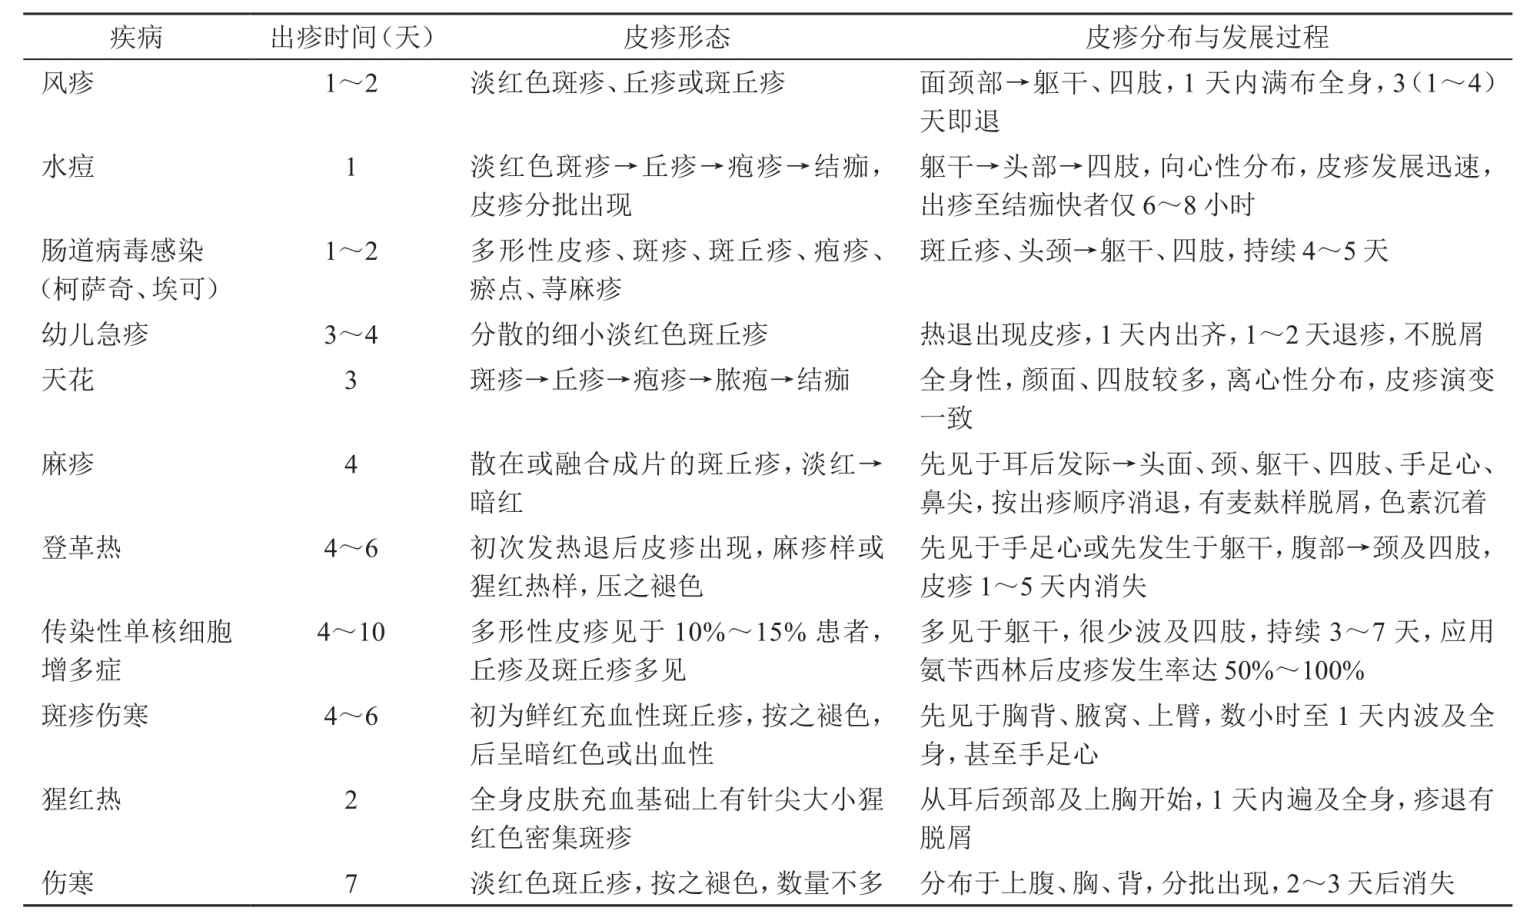
\includegraphics[width=6.625in,height=3.95833in]{./images/Image00003.jpg}
\end{table}

\subsubsection{病因诊断}

发热是由于各种原因导致机体产热过多或散热减少,以及体温中枢功能障碍所致。其原因很多且复杂。在临床实践中,以发热为主诉或唯一症状就诊者有急性发热,尤其出疹性发热,原因不明发热,长期低热,超高热与反复发热。其病因特征亦各异。

\paragraph{急性发热}

热程在2周以内的发热称为急性发热。其原因很多,绝大多数属于感染,尤以呼吸道、泌尿道和消化道感染最常见,因为这些系统与外界相通,最易遭受病原体的侵袭。在排除上述系统感染后,则要注意某些急性传染病和其他系统的感染。一般而言,这类发热,常伴有定位症状,比较容易诊断。

\paragraph{长期}

“不明原因”的中、高热
系指发热持续3周以上,体温多次超过38.3℃,经过至少1周深入细致的检查仍不能确诊的一组疾病,称为原因不明发热(fever
of unknown
origin,FUO)。其病因在不同年代和不同地理区域明显不同,但主要有感染、恶性肿瘤与结缔组织-血管性疾病三大类,共约占长期发热病因的80\%~90\%。其中由感染引起的长期发热在国内占60\%~70\%,在其他发展中国家更高些,而在发达国家约占总数1/3。由于人的寿命延长,传染病逐渐减少,恶性肿瘤引起的发热比例有增高趋势,国内约占20\%。结缔组织-血管性疾病约占10\%。病因也受年龄的影响:6岁以下的FUO患儿以感染性疾病为主,尤其是原发性上呼吸道、泌尿道感染或全身感染;6~14岁年龄组则以结缔组织-血管性疾病和小肠炎症性疾病为最常见的病因;14岁以上的成人组,虽然仍以感染性疾病占首位,但肿瘤性疾病明显增多。仍有10\%的病例始终原因不明。

\hypertarget{text00008.htmlux5cux23CHP1-1-2-4-2-1}{}
(1) 感染:

引起发热待查的感染性疾病中主要由细菌感染所致,而任何一种致病菌或条件致病菌,或L-型细菌性感染均可分为全身性与局部性感染。全身性感染以伤寒与副伤寒、粟粒型结核与播散性结核(包括腹膜、肠、肠系膜淋巴结、肝、肾、胸膜和肺与肺门淋巴结结核)、脓毒症与感染性心内膜炎、布鲁菌病、黑热病、急性血吸虫病、旋毛虫病等;局部性感染以肝脓肿、胆道与泌尿生殖道感染、腹腔内脓肿(包括肝下、膈下、结肠旁、阑尾周围、腹膜后、盆腔脓肿等)为常见。局部性感染易被临床忽略。

\hypertarget{text00008.htmlux5cux23CHP1-1-2-4-2-2}{}
(2) 恶性肿瘤:

也是长期发热的常见原因。最常见的为原发性肝癌、淋巴瘤、恶性组织细胞病与白血病,其次为实质性恶性肿瘤如肺癌、肾癌、甲状腺癌等。

\hypertarget{text00008.htmlux5cux23CHP1-1-2-4-2-3}{}
(3) 结缔组织-血管性疾病:

也是较常见原因之一,大多伴有关节痛、皮肤、心、肾等多系统病变引起的相应症状与体征,但少数病例在典型症状出现前数周或数月可出现发热。此类疾病以系统性红斑狼疮、成人少年型类风湿关节炎、多动脉炎、皮肌炎、混合性结缔组织病、风湿热等常见。

\hypertarget{text00008.htmlux5cux23CHP1-1-2-4-2-4}{}
(4) 其他:

肉芽肿性疾病(肉芽肿性肝炎、结节病、局限性回肠炎等)、药物热、伪装热、体腔积血如血胸、血腹、肺梗死等。

\paragraph{长期低热}

系指口腔温度在37.5~38.4℃,持续4周以上者。在诊断为长期低热时,必须先了解其正常体温,排除生理或功能性因素,并排除高温环境等影响,如在高温车间的纺织女工中,有长期低热者可达10\%以上。长期低热由感染性疾病引起者占40\%,非感染性疾病占57\%,原因不明占3\%。长期低热的原因可分为器质性与功能性两大类:

\hypertarget{text00008.htmlux5cux23CHP1-1-2-4-3-1}{}
(1) 器质性低热:

①慢性感染:如结核病、肝脏疾病、慢性肾盂肾炎、慢性胆道感染以及各种病灶感染(鼻窦炎、牙根脓肿、前列腺炎、慢性盆腔炎、肛门周围脓肿等)。②结缔组织疾病:如风湿热、类风湿关节炎、系统性红斑狼疮等。③内分泌疾病:如甲亢、嗜铬细胞瘤等。④恶性肿瘤:早期淋巴瘤、实质性癌肿转移等。

\hypertarget{text00008.htmlux5cux23CHP1-1-2-4-3-2}{}
(2) 功能性低热:

①生理性低热:月经前期低热、妊娠期低热等。②神经功能性低热:多见于青年女性,长期低热可长达数月或数年。有些患者低热有季节性,出现于夏季(谓之夏季低热),且每年如此。体温在一昼夜内波动幅度较小,常不超过0.5℃,且口腔、腋窝与直肠温度差不大,甚至可出现腋温大于口温,口温大于肛温或腋温大于肛温的反常现象,两侧腋温可相差1℃以上。体温昼夜规律失常。患者常伴有脸色潮红、皮肤划痕症、心动过速等自主神经功能紊乱或神经症色彩。但患者一般情况好,体重无变化,虽经各种药物治疗无效,但不经治疗也可自行消退。神经功能性低热较常见,约占长期低热的1/3,预后良好。③感染后低热:急性病毒或细菌感染得到控制后,高热消退,但可出现持续较久的低热,并伴有乏力,纳差等现象。此种发热可能与体温调节中枢功能失常或自主神经功能紊乱有关。

\subsubsection{超高热危象的识别与诊断}

超高热系指发热超过41℃以上,主要见于体温调节中枢功能障碍,有以下各种原因:①中暑或日射病;②脑部疾病:如严重脑外伤、脑出血、脑炎与脑肿瘤等;③输血、输液污染引起严重致热原反应与脓毒症;④麻醉药引起的恶性高热;⑤临终前超高热等。不论病因如何,超高热对细胞膜与细胞内结构有直接损害作用,当深部体温>
41℃时细胞线粒体的氧化磷酸化出现障碍,可引起永久性脑损害;42~43℃持续数分钟细胞会陷入不可逆的损害,涉及全身各种细胞,尤以脑、心、肝、肾的变化最为突出,容易造成脑水肿颅内压升高,抽搐、昏迷,心、肝、肾、肺功能衰竭,DIC等多脏器功能衰竭。超高热危象的诊断要点是:

\paragraph{超高热}

超高热(体温> 41℃)是超高热危象的必有表现。

\paragraph{超高热时伴有多脏器功能受损害的表现}

①心血管系统:低血压休克、心功能不全、心肌缺血与心律失常等。②中枢神经系统:体温越高对中枢神经系统损害越重,症状出现越早;包括不同程度的意识障碍如谵妄、嗜睡、昏迷、抽搐、大小便失禁、脑膜刺激征、瘫痪、病理反射阳性、脑疝、视神经乳头水肿等。③凝血功能障碍:早期出现凝血酶原时间延长,纤维蛋白原减少,血小板减少,出血时间、凝血时间延长;晚期常有广泛而严重的出血、DIC形成。这与过高热直接损害毛细血管、渗透性增加,肝功能受损凝血因子减少,骨髓受损血小板减少等有关。④肾功能损害:可有血尿、管型、少尿、无尿、血肌酐升高等肾功能不全的表现。⑤肝功能损害:肝功能异常如ALT升高、血清胆红素升高,甚至表现为急性肝功能衰竭。⑥水电解质和酸碱平衡失调。⑦其他表现:如横纹肌溶解可致血肌酸磷酸激酶(CK)增高等。

\paragraph{原发病的表现}

如中毒性菌痢的腹泻、脓血便;乙脑时的抽搐、昏迷等。

\subsection{处理原则}

\paragraph{支持治疗}

患者出现神志改变、呼吸窘迫、血流动力学不稳定等危及生命的症状与体征时,立即实施监护、建立静脉通路、气道管理、补液以及氧疗,必要时予以呼吸支持治疗。

\paragraph{超高热危象的处理}

超高热和超高热危象是短暂的临床表现,经适当处理可能很快恢复(如中暑、输液反应等),亦可很快死亡(恶性高温)。早期诊断与早期处理同预后直接有关。因此,对每个可能发生超高热的患者应随时检测体温,一旦出现超高热,应以最快的速度降低中心体温、代谢率,以打断超高热引起的恶性循环,同时防治各种并发症。其中,降温是抢救超高热危象的主要措施。降温速度决定预后,应在1小时内使直肠温度降至38.5℃以内。具体降温措施详见本书第129章“中暑”。

\paragraph{对症处理}

发热的对症治疗包括:①物理降温:一般可用冷毛巾湿敷额部,每5~10分钟更换1次,或用冰袋置于额、枕后、颈、腋和腹股沟处降温,或用25\%~50\%酒精擦浴。或头置冰帽、冰水灌肠、冷盐水洗胃,或将患者置于空调房内(使室温维持在27℃左右)。应根据具体条件选用。②药物降温:视发热程度可采用口服或肌注解热镇痛药。常用的口服解热镇痛药有:阿司匹林(0.3~0.6g/次)、对乙酰氨基酚(0.3~0.5g/次)、布洛芬(0.2~0.4g/次)、安乃近(0.25~0.5g/次)、解热止痛片(APC片,1~2
片/次)、速效伤风胶囊(1~2粒/次)、复方对乙酰氨基酚片(1~2片/次)等。常用的注射用解热镇痛药有:阿司匹林精氨酸盐(0.5~1.0g/次)、阿司匹林赖氨酸盐(赖氨匹林,0.9~1.8g/次)、对乙酰氨基酚(0.15~0.25g/次)、息热痛注射液(2ml/次)、安痛定注射液(1支/次)等。高热者病情需要时可短期应用肾上腺皮质激素,如地塞米松5~10mg静注或肌注;或以地塞米松12~20mg/d或氢化可的松300~600mg/d静滴。

\paragraph{抗生素经验性应用}

对感染病例早期抗生素经验性应用是有益的。一般来讲,若有明确的病原菌感染,则选择覆盖特定病原菌感染的窄谱抗生素;若不明确,可选择覆盖革兰阳性和革兰阴性需氧菌、厌氧菌的广谱抗生素。

\paragraph{诊断性治疗}

当发热病因一时难以查明时,在不影响进一步检查的情况下,可按可能性较大的病因进行诊断性治疗(如疑疟疾,可试用氯喹;疑阿米巴性肝脓肿,行抗阿米巴治疗;疑结核病行抗结核治疗时间以3~4周以上为宜),期望获得疗效而做出临床诊断。诊断性治疗应选用特异性强、疗效确切及安全性大的治疗药物,剂量应充足并完成整个疗程,无特殊原因不得随便更换试验药物。

\paragraph{随访观察}

对部分症状轻微、经过详细检查仍不能明确病因的发热待查患者,也可在专科门诊进行长期随访而不作特殊处理,确有不少患者可获自愈。

\protect\hypertarget{text00009.html}{}{}

\hypertarget{text00009.htmlux5cux23CHP1-1-4}{}
参 考 文 献

1. 陈灏珠 ,林果为.实用内科学.第13版.北京:人民卫生出版社,2009:332

2. 陈文彬 ,潘祥林.诊断学.第7版.北京:人民卫生出版社,2008:16

3.
陈新谦,金有豫,汤光.新编药物学.第17版.北京:人民卫生出版社,2011:179

\protect\hypertarget{text00010.html}{}{}

\chapter{意识障碍和昏迷}

意识是指人体对周围环境及自身状态的感知能力。意识障碍(disturbance of
consciousness)是脑和脑干功能活动的抑制状态。按照生理与心理学基础可将意识障碍分为觉醒障碍(觉醒度下降,即狭义的意识障碍)和意识内容障碍两大类。前者表现为嗜睡、昏睡和昏迷;后者表现为意识模糊和谵妄等。脑和脑干功能活动的不同抑制程度决定了不同的意识障碍水平。

昏迷(coma)是一种最为严重的意识障碍。患者意识丧失,运动、感觉、反射和自主神经功能障碍,给予任何刺激(如语言、声音、光线、疼痛等)均不能将患者唤醒,但生命体征如呼吸、脉搏、心跳、血压和体温尚可存在。昏迷是病情危重的信号,是常见危重急症,病死率高,临床医师如能迅速作出正确的诊断和及时的处理,患者往往可能转危为安。

以觉醒度改变为主的意识障碍,根据检查时刺激的强度和患者的反应,可分为以下三级:

嗜睡(drowsiness):主要表现为病理性睡眠过多过深,能被各种刺激唤醒,并且能够正确回答问题和做出各种反应,但当刺激去除后又很快入睡。

昏睡(stupor):是一种比嗜睡深而又较昏迷稍浅的意识障碍。昏睡时觉醒水平、意识内容及随意运动均减至最低限度。患者不能自动醒转,在持续强烈刺激下能睁眼、呻吟、躲避,可作简短而模糊的回答,但反应时间持续很短,很快又进入昏睡状态。昏睡时可见到运动性震颤、肌肉粗大抽动、不宁或刻板的动作、强握和吸吮反射。

昏迷(coma):患者意识完全丧失,各种强刺激不能使其觉醒,无有目的的自主活动,不能自发睁眼。昏迷按严重程度可分为浅昏迷、中昏迷和深昏迷三级:①浅昏迷(mild
coma):即轻度昏迷。仅对剧痛刺激(如压迫眶上神经)有防御性反应和痛苦表情,不能言语,可有无意识的自发动作,各种生理反射存在(如吞咽、咳嗽、角膜和瞳孔对光反射),呼吸、血压、脉搏一般无明显改变。②中昏迷:对外界的正常刺激均无反应,自发动作很少。对强烈刺激可有防御反射,角膜反射减弱,瞳孔对光反射迟钝,眼球无转动,大小便潴留或失禁。呼吸、血压、脉搏已有变化。③深昏迷(deep
coma):对外界的任何刺激均无反应,全身肌肉松弛,无任何自主运动。眼球固定,瞳孔散大,各种反射全部消失,大小便多失禁。生命体征已有明显改变,呼吸不规则,血压或下降。

以意识内容改变为主的意识障碍常见有以下三种:

意识模糊(confusion):表现为注意力减退,情感反应淡漠,定向力障碍,活动减少,语言缺乏连贯性,对外界刺激可有反应,但低于正常水平。

精神错乱(psychoderangement):患者对周围环境的接触程度障碍,认识自己的能力减退,思维、记忆、理解与判断力均减退,言语不连贯并错乱,定向力亦减退。常有胡言乱语、兴奋躁动。

谵妄状态(delirium):表现为意识内容清晰度降低,伴有睡眠-觉醒周期紊乱和精神运动性行为。除了上述精神错乱以外,尚有明显的幻觉、错觉和妄想。幻觉以视幻觉最为常见,其次为听幻觉。幻觉的内容极为鲜明、生动和逼真,常具有恐怖性质。因而,患者表情恐惧,发生躲避、逃跑或攻击行为,以及运动兴奋等。患者言语可以增多,不连贯或不易理解,有时则大喊大叫。谵妄或精神错乱状态多在晚间加重,也可具有波动性,发作时意识障碍明显,间歇期可完全清楚,但通常随病情变化而变化,持续时间可数小时、数日甚至数周不等。

\subsection{病因与发病机制}

意识是大脑功能活动的综合表现,是人对自身及外界环境进行认识和做出适宜反应的基础,包括觉醒状态与意识内容两个组成部分。觉醒状态是指与睡眠呈周期性交替的清醒状态,由脑干网状激活系统和丘脑非特异性核团维持和激活,属皮质下激活系统的功能;意识内容是指人的知觉、思维、情绪、记忆、意志活动等心理过程(精神活动),还有通过言语、听觉、视觉、技巧性运动及复杂反应与外界环境保持联系的机敏力,属大脑皮质的功能。正常意识是指觉醒水平与意识水平都处于正常状态,表现为对自身与周围环境有正确理解,对内外环境的刺激有正确反应,对问话的注意力、理解程度以及定向力和计算力都是正常的。脑电生理正常。意识障碍是脑和脑干功能活动的抑制状态,表现为人对自身及外界认识状态以及知觉、记忆、定向和情感等精神活动不同程度的异常。尽管痴呆、冷漠、遗忘、失语等,都是意识内容减退的表现,但只要在其他行为功能还能作出充分和适当的反应,就应该认为意识还是存在的。

正如上述,意识是人对自身及外界环境进行认识及作出适宜反应的基础。意识的“开关”系统包括特异性和非特异性上行投射系统。特异性上行投射系统是各种感觉传入通路的总称。人体通过各种感觉器官接受躯体感觉冲动,经各传导束终止于丘脑特异性核团,再投射到大脑皮质相应的感觉区,引起大脑皮质的激醒。上述感觉冲动途经脑干时发出侧支至脑干网状结构,后者弥散地作用于整个大脑皮质,使大脑皮质处于觉醒状态,称为上行网状激活系统(ascending
reticular activity
system,ARAS)。丘脑下部则接受来自内脏的感觉冲动及体液性刺激,激活大脑边缘系统,称为丘脑下部激活系统,它与ARAS在功能上具有密切联系。大脑皮质受到这两种激活系统的调节与维持,保持觉醒状态。大脑皮质又通过皮质网状束的离皮质联系(corticofugal
connection)向网状结构传递反馈神经冲动,以调节ARAS的活动。这一反馈环路的神经冲动,循环不已,从而维持大脑皮质的持久清醒和意识活动。因此,凡ARAS、丘脑、丘脑下部激活系统或大脑皮质发生器质性或可逆性病变时,均可引起意识障碍。一般当损害或抑制脑干网状结构时引起觉醒障碍;双侧大脑半球的广泛损害或功能抑制可引起意识障碍或昏迷;一侧大脑半球的急性广泛病变,尤其是在优势侧半球,亦可发生意识障碍。颅内局灶病变一般不引起意识障碍,但病变发展迅速并伴有脑循环障碍、脑水肿、颅内高压等时,也可引起不同程度的意识障碍。病变侵犯间脑也可早期发生意识障碍,并且迅速发展。缓慢发展的大脑局灶病变一般无意识障碍,但如合并脑疝,患者可迅速陷入昏迷。不同的病因和病变部位,引起昏迷的发病机制也有差异,详见表\ref{tab2-1}和表\ref{tab2-2}。

\subsection{诊断思路}

任何原因所致的弥漫性大脑皮质和(或)脑干网状结构的损害或功能抑制均可造成意识障碍和昏迷。临床上,引起意识障碍和昏迷的具体病因很多,通过病史和临床检查,有的病因易明确,有的则不易明确。因此,必须边询问病史,边体检,边观察,边治疗。并就以下问题进行分析和判断:①是不是昏迷?②昏迷的程度如何?③引起昏迷的病因是什么?是颅内疾病抑或全身性疾病?若是前者,是颅内局限性病变抑或弥漫性病变?如系局限性病变,它是位于幕上抑或幕下?具体病因是什么?若是全身性疾病,具体病因是什么?

\subsubsection{病史与体检}

对意识障碍和昏迷患者的诊断需要详询病史,仔细而全面的体检以及必要的实验室或特殊辅助检查。

\hypertarget{text00010.htmlux5cux23CHP1-2-2-1-1}{}
(一) 病史采集

对意识障碍和昏迷患者
,采集病史要简明扼要。病史中应着重了解:①发生意识障碍和昏迷的时间、诱因、起病缓急、方式及其演变过程等。②意识障碍和昏迷的伴随症状以及相互间的关系:如首发症状为剧烈头痛者要考虑蛛网膜下腔出血、脑出血、脑膜炎;高热、抽搐起病者结合季节考虑乙型脑炎、流行性脑脊髓膜炎;以精神症状开始者应考虑脑炎、额叶肿瘤等;老年患者以眩晕起病要考虑小脑出血或椎-基底动脉系的缺血。③意识障碍和昏迷发生前有无服用药物(如镇静安眠药、抗精神病药、降血糖药等)、毒物和外伤史,既往有无类似发作等。④既往有无癫痫、精神疾患、长期头痛、视力障碍、肢体运动受限、高血压和严重的肝、肾、肺、心脏疾患以及内分泌代谢疾病等。⑤了解发病现场和环境:如有无未服完的药品、呕吐物;有无特殊气味(如CO、硫化氢等);季节特点(如寒冷、高温等);附近有无高压电线。

\hypertarget{text00010.htmlux5cux23CHP1-2-2-1-2}{}
(二) 体格检查

包括体温
、脉搏、呼吸、血压和皮肤黏膜,以及神经系统以外的其他系统检查等。

\paragraph{体温}

①体温升高:常见于严重的颅内外感染性疾病(脑炎、脑膜炎、肺部感染、脓毒症等)、脑出血、蛛网膜下腔出血、中暑等。高热无汗还应考虑是否有抗胆碱能药物中毒。②体温降低:常见于酒精中毒、一氧化碳中毒、休克、镇静催眠药中毒、低血糖昏迷、黏液性水肿、垂体功能减退、艾迪生病及下位脑干的广泛损害和冻僵等。

\begin{table}[htbp]
\centering
\caption{颅内疾病引起昏迷的病变部位、发病机制、临床表现和常见病因}
\label{tab2-1}
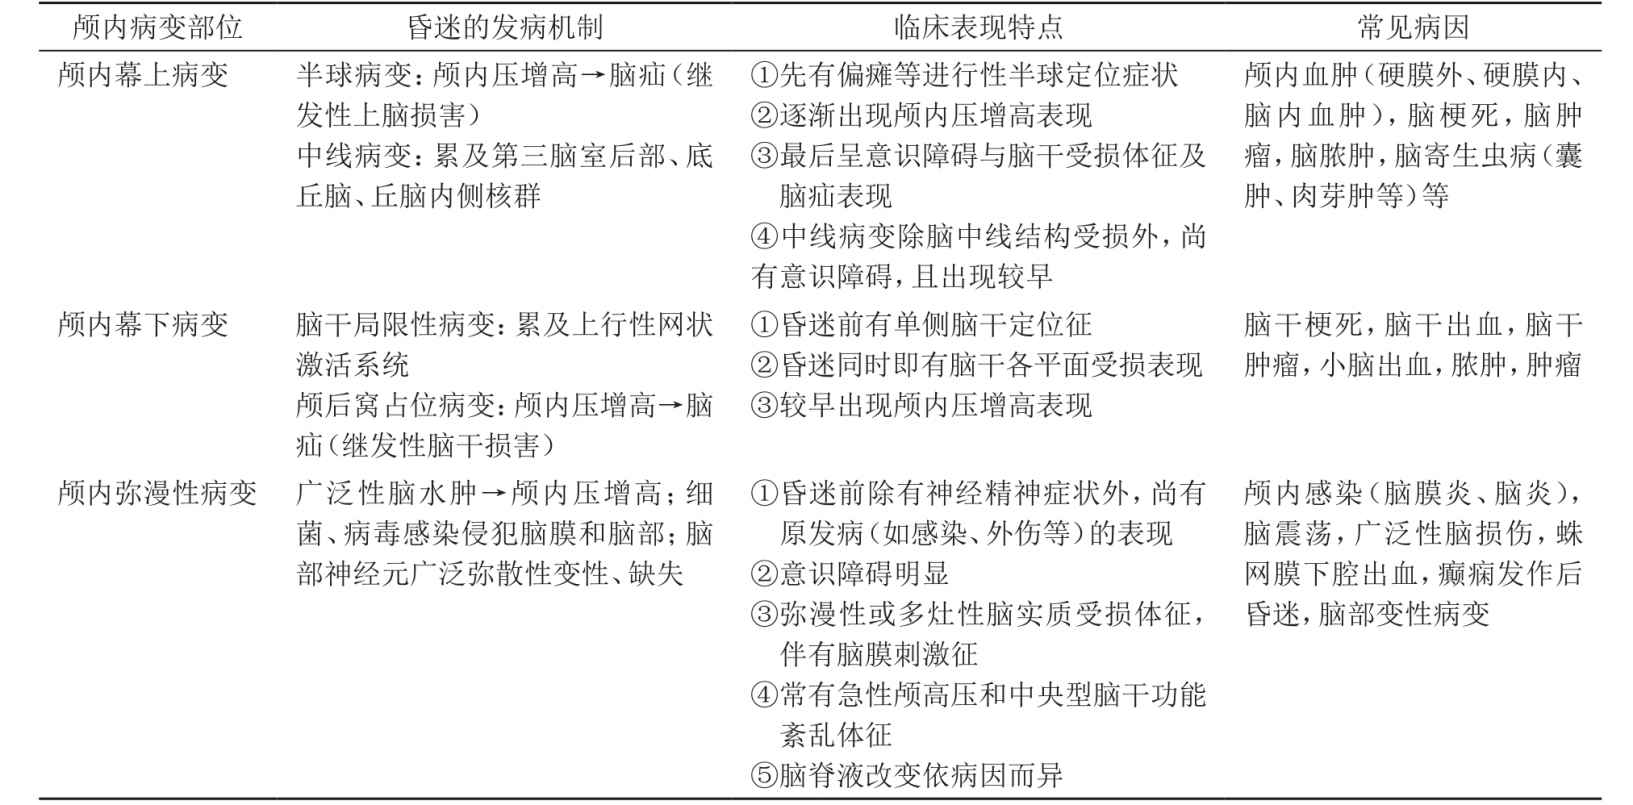
\includegraphics[width=6.73958in,height=3.32292in]{./images/Image00004.jpg}
\end{table}

\begin{table}[htbp]
\centering
\caption{引起昏迷的全身性疾病及其分类、发病机制和常见病因}
\label{tab2-2}
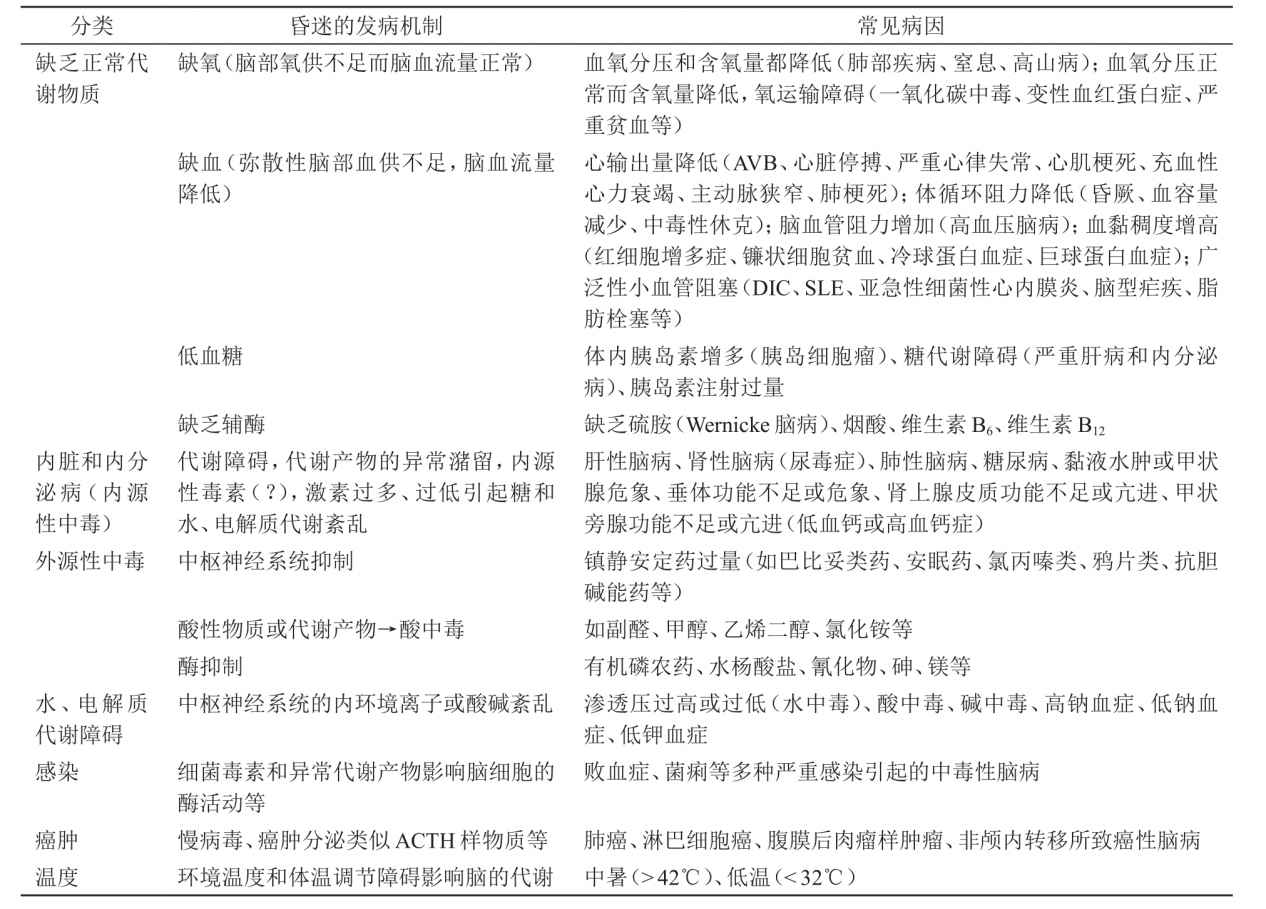
\includegraphics[width=6.73958in,height=4.83333in]{./images/Image00005.jpg}
\end{table}

\paragraph{脉搏}

脉搏触诊有助于及时发现急性心源性脑缺血综合征。脉慢而洪大见于脑出血、酒精中毒;脑脓肿患者的脉搏常缓慢、充实而规则;而脑膜炎患者的脉搏多细速。颠茄类、氯丙嗪中毒时脉搏显著增快。脉搏先慢后快,同时伴有血压下降者,可见于脑疝压迫脑干、延髓生命中枢衰竭,提示预后不良。

\paragraph{呼吸}

观察患者的呼吸方式、节律和频率等。呼吸深而快,常见于代谢性酸中毒(糖尿病、尿毒症等);鼾声呼吸且伴有呼吸时一侧面肌瘫痪者提示脑出血。浅而快速的规律性呼吸见于休克、心肺疾患或镇静催眠药中毒引起的呼吸衰竭,肺炎等缺氧性疾病可伴发绀和鼻翼扇动;呼吸深而慢、同时脉搏慢而有力和血压增高,为颅内压增高的表现。呼吸过慢并伴有叹息样呼吸常为吗啡类药物中毒。呼气带有氨味见于尿毒症昏迷;带有苹果味见于糖尿病昏迷;苦杏仁气味提示氢氰酸(苦杏仁、木薯、氰化物等)中毒;呈酒味提示酒精中毒;呼气及排泄物有大蒜样臭味可见于有机磷农药中毒;呼气中及尿液出现“肝臭”者提示肝性脑病。

昏迷患者呼吸节律的异常类型常常提示脑部病变的部位,与神经功能障碍水平定位有密切关系。双侧额叶损害可出现过度换气后呼吸暂停(PHVA)现象,即每在5~10次深呼吸后呼吸暂停。脑部广泛病损使中脑内呼吸中枢失去大脑的控制时,可出现潮式呼吸,即陈-施呼吸(Cheyne-Stokes
respiration,CSR),表现为呼吸由浅慢逐渐变为深快,再由深快变为浅慢,随后出现一段呼吸暂停后,然后重复上述周期性呼吸。潮式呼吸的周期可以长达30秒~2分钟,暂停时间可长达5~30秒。当中脑和脑桥上部功能受损后,可出现中枢神经源性过度呼吸(central
neurogenic
hyperventilation,CNH),呼吸深、快、均匀、持久,频率达40~70次/分。脑桥下部损害后可出现:①喘息样呼吸(gasping
of
breaths),常在濒死时出现,表现为深呼吸、较慢的频率,跳跃式深吸气,呼吸暂停6~10秒,可见于延髓内肿瘤或严重的药物中毒时;②交替呼吸,表现为一次强呼吸和一次弱呼吸交替;③间歇(Biot)呼吸,表现为每3~4次呼吸后出现呼吸暂停;④长吸式呼吸(apneustic
breathing),是一种吸气持续的延长性吸气痉挛,吸2~3次呼1次或吸足气后呼吸暂停。所谓鱼嘴式呼吸(每次吸气时下颌张开似鱼嘴),亦见于脑干下部损害时,常为预后严重的征兆。延髓受损时,呼吸紊乱更为严重,频率和幅度均不时改变,间以不规则地呼吸中断,有人亦称其为“共济失调性呼吸”(ataxic
breathing),最后发展至呼吸完全停止。在天幕上占位病变发展至出现天幕裂孔疝和枕大孔疝的过程中,有时可见到呼吸形式的一系列改变(潮式呼吸→中枢神经源性过度呼吸→喘息式呼吸→共济失调性呼吸),提示脑干功能自首端向尾端逐渐发生障碍。

\paragraph{血压}

血压显著增高,见于脑出血、高血压脑病、颅内压增高等;血压过低常见于糖尿病昏迷、酒精中毒、巴比妥类药物中毒等。

\paragraph{皮肤黏膜}

皮肤灼热干燥见于中暑高热;皮肤湿润多汗见于低血糖昏迷、有机磷农药中毒等;皮肤苍白常见于尿毒症性、低血糖性昏迷等;皮肤潮红见于脑出血、颠茄类中毒及酒精中毒;口唇发绀为严重缺氧如窒息、自缢或肺性脑病等;口唇樱红考虑一氧化碳中毒、严重酸中毒;口角见到单纯疱疹,考虑为疱疹性脑炎、脑型疟疾、大叶性肺炎或流脑等;皮肤巩膜黄染应考虑肝性脑病或药物中毒;昏迷伴有结合膜瘀斑、皮疹、皮肤瘀斑,须鉴别脓毒症、流脑、流行性出血热等引起的昏迷;有无头部、颜面部皮肤损伤的痕迹,有无舌咬伤、耳鼻部出血、脑脊液漏、耳后及皮下出血等,对诊断颅骨骨折、颅脑外伤及癫痫大发作常有帮助;颈部手术瘢痕可能提示甲状腺或甲状旁腺疾患,电解质不平衡或内分泌功能障碍;胸腔手术或乳房手术瘢痕应想到颅内转移或伴随于恶性肿瘤的高钙血症、低钠血症等电解质紊乱。应注意肢体、皮肤上成串的针疤或皮下脓肿可能曾滥用药物。

\hypertarget{text00010.htmlux5cux23CHP1-2-2-1-3}{}
(三) 神经系统检查

意识障碍时神经系统查体主要包括以下几个方面的检查
:眼征、对疼痛刺激的反应、瘫痪体征、脑干反射、锥体束征和脑膜刺激征等。

\paragraph{眼征}

包括以下几个方面:

\hypertarget{text00010.htmlux5cux23CHP1-2-2-1-3-1-1}{}
(1) 瞳孔变化:

观察瞳孔的大小、形状、位置、双侧对称性及对光反应,可帮助判断神经损害的部位及程度。①瞳孔对光反射:为光线刺激瞳孔引起的缩瞳反射。其传导径路为:视网膜→视神经→中脑被盖前区→埃-魏核→动眼神经→膝状神经节→颈上交感神经节节后纤维→瞳孔括约肌,径路上任何一处损害均可引起对光反射丧失和瞳孔散大。瞳孔对光反射与昏迷程度成正比(但巴比妥类中毒虽呈深昏迷,对光反射却残存是特征)。②瞳孔改变与病因:单侧瞳孔扩大,除外药物作用,昏迷患者单侧瞳孔扩大(≥5mm)者,可定为视神经损害或动眼神经损害造成。视神经损害常由于急性颅脑外伤伴发视神经损伤,有球后视神经炎过去史,或局部肿瘤或动脉瘤压迫引起单侧性黑矇性瞳孔麻痹,同侧直接光反射及对侧间接光反射消失;视神经萎缩者,亦可见该侧瞳孔扩大。动眼神经损害单侧瞳孔扩大,多见于后交通动脉瘤破裂引起的蛛网膜下腔出血,也可见于颞叶钩回疝、颅脑外伤伴发硬膜外血肿、脑出血、脑肿瘤等压迫。颈内动脉血栓形成,大脑中动脉浅支或深支梗塞时,亦可见单侧瞳孔扩大。个别癫痫患者抽搐后出现暂时性单侧瞳孔扩大,机制不明。双侧瞳孔扩大,可见于药物或食物中毒如颠茄类、巴比妥类(有时缩小)、氰化物、肉毒杆菌中毒等;脑疝进行到晚期瞳孔由单侧扩大扩展为双侧扩大,昏迷加深,提示预后不良。天幕上病变尚未引起脑疝或中脑结构移位时,瞳孔大小接近正常,若发生小脑幕切迹疝,则见病灶侧瞳孔扩大,对光反射消失,若观察脑疝形成的全过程,则可发现扩大侧瞳孔先有缩小的改变(由于动眼神经的压迫与牵拉,病侧缩瞳纤维首先受到刺激,继而麻痹)。单侧瞳孔缩小较少见,上述幕上占位病变导致早期颞叶钩回疝时,可见同侧瞳孔缩小,而光反射存在;脑干梗死也可见到一侧瞳孔缩小(霍纳综合征表现之一)。双侧瞳孔缩小,可见于氯丙嗪、吗啡类药物、有机磷农药、水合氯醛、毒蕈等中毒与尿毒症;双侧瞳孔缩小如针眼,伴有高热是原发性脑桥出血的特征,若患者还有四肢阵发性强直性抽搐则是脑室出血的表现。中央型间脑疝而致双侧下丘脑损害可出现双侧瞳孔缩小。

\hypertarget{text00010.htmlux5cux23CHP1-2-2-1-3-1-2}{}
(2) 眼球运动:

眼球运动受大脑皮质、脑桥、中脑和第3、4、6脑神经控制,其运动异常有重要的定位意义。在代谢性脑病中,仅巴比妥类和苯妥英钠中毒可有眼球运动障碍。若患者的眼球和浅睡眠一样,能缓慢地向两侧转动,说明脑桥和中脑的有关功能尚相对地完好,据此可推测天幕下病变引起的昏迷可能性较小。一侧大脑半球有较广泛的损害时,患者双眼常偏向瘫痪肢体的对侧;一侧脑桥受损时,则双眼偏向肢体瘫痪的同侧。在双侧大脑皮质急性病变时,可见到有眼球激动现象,每隔几秒钟双眼出现强烈的快速摆动。丘脑底部和上位中脑损害患者,眼球可能向下和向内转,就像盯着自己鼻尖看。眼球浮动(ocular
bobbing)是双眼球快速同向下转后又缓慢地向上转恢复至原位,每分钟重复2~3次,转动的幅度约1~3mm,它发生于眼球水平向运动机制被破坏的情况,其机制为脑桥侧视中枢受损,而中脑的眼球垂直运动中枢未受损之故,见于脑桥的双侧性损害。脑干广泛严重损害时,眼球运动完全丧失而固定在正中位。垂直性眼球运动障碍如双眼向上或向下凝视,提示中脑四叠体附近或下丘脑病变;分离性眼球运动可为小脑损害表现。

\hypertarget{text00010.htmlux5cux23CHP1-2-2-1-3-1-3}{}
(3) 眼底检查:

凡是能引起颅内压增高的疾病均可引起眼底改变。颅脑外伤或颅内出血后12~24小时即可出现视神经乳头水肿的变化;但严重的视乳头水肿多数是由于长期颅内压增高的后果,应考虑有脑肿瘤、脑脓肿等占位病变的可能。如视网膜有广泛的渗出物、出血,则应考虑有糖尿病、尿毒症、高血压脑病等可能。玻璃体下较大的或视网膜广泛的浅表出血通常见于蛛网膜下腔出血。

\paragraph{对疼痛刺激的反应}

用力按压眶上缘、胸骨检查昏迷患者对疼痛的运动反应,有助于定位脑功能障碍水平或判断昏迷的程度。出现单侧或不对称性姿势反应时,健侧上肢可见防御反应,病侧则无,提示瘫痪对侧大脑半球或脑干病变。观察面部疼痛表情时,可根据面肌运动,判断有无面瘫。疼痛引起去皮质强直(decorticate
rigidity),表现为上肢内收和屈曲,下肢伸直,与丘脑或大脑半球病变有关;去脑强直(decerebrate
rigidity)表现为四肢伸直,肌张力增高或角弓反张,提示中脑功能受损,较去皮质强直脑功能障碍程度更为严重。脑桥和延髓病变患者通常对疼痛无反应,偶可发现膝部屈曲(脊髓反射)。

\paragraph{瘫痪体征}

意识障碍和昏迷患者的瘫痪检查,可通过疼痛刺激观察面部表情与肢体活动,以及肢体坠落试验等来判定。①观察面颊:一侧面瘫时,可见该侧鼻唇沟变浅,口角低垂,睑裂增宽,呼气时面颊鼓起,吸气时面颊塌陷,呈吸烟斗动作。②疼痛刺激:压迫眶上切迹或捏掐肢体,观察患者肢体活动情况,瘫痪侧少动或不动。③观察双眼球共同偏视(见前述)。④胸骨反射:针刺胸骨柄部,引起一侧或双侧上肢的屈曲反应,手移向胸骨部,刺激加重,可波及下肢。一侧肢体反射消失或运动反应弱,提示该侧肢体瘫痪。⑤上肢坠落试验:将患者双上肢抬起,使与躯干呈垂直位,突然放手,观察肢体坠落情况,瘫痪肢体迅速坠落而且沉重,无瘫痪肢体则向外侧倾倒,缓慢坠落。⑥下肢坠落试验:将患者下肢膝部屈曲抬高,足跟着床,突然松手时,瘫痪侧肢体不能自动伸直,并向外侧倾倒;无瘫痪肢体则呈弹跳式伸直,并能保持足垂直位。⑦足外旋试验:先将患者的双下肢伸直放平,然后把双足扶直并拢,突然松开时,则瘫痪肢体的足立刻外旋倾倒,足外缘着床;无瘫痪的足,仍能维持足垂直位。⑧反射的改变:瘫痪肢体侧常伴有中枢性面瘫,腹壁、提睾反射减弱或消失,腱反射增强,病理反射阳性。

\paragraph{脑干反射}

可通过睫脊反射(ciliospinal reflex)、角膜反射(corneal
reflex)、头眼反射(oculocephalic reflex)和眼前庭反射(oculovestibular
reflex)等脑干反射来判断是否存在脑干功能损害。反射性眼球运动包括头眼反射和眼前庭反射。

\hypertarget{text00010.htmlux5cux23CHP1-2-2-1-3-4-1}{}
(1) 睫脊反射:

给予颈部皮肤疼痛刺激时可引起双侧瞳孔散大,此反射存在提示下位脑干、颈髓、上胸段脊髓及颈交感神经功能正常。

\hypertarget{text00010.htmlux5cux23CHP1-2-2-1-3-4-2}{}
(2) 角膜反射:

角膜反射是由三叉神经的眼神经与面神经共同完成的,当三叉神经的第一支(眼神经)或面神经损害时,均可出现角膜反射消失。若脑桥上部和中脑未受累及,角膜反射存在;一侧角膜反射消失见于同侧面神经病变(同侧脑桥),双角膜反射消失见于一侧三叉神经受损或双侧面神经受损,提示中脑或脑桥受累,常有意识障碍。

\hypertarget{text00010.htmlux5cux23CHP1-2-2-1-3-4-3}{}
(3) 头眼反射:

又称玩偶眼试验(Doll's eye
test)。在浅昏迷患者,检查者使其眼睑睁开,并将患者的头向两侧或前后转动,先慢后快,患者双眼反射地朝与头转动相反的方向转动(如头转向右侧时,双眼凝视偏向左侧),谓之头眼反射(本体觉转头反射、环偶眼现象)阳性。在婴儿为正常反射,随着大脑发育而抑制。头眼反射的刺激主要通过颈部肌肉本体觉,通过本体觉神经纤维进入脊髓,先经过颈髓2~4节段的背根,然后进入颈髓再上升达到延髓前庭神经核、中脑顶盖部、脑桥,以及第3、4、6脑神经。正常人清醒状态下,头眼反射为大脑半球发起的视觉固定(或注视,visual
fixation)所抑制,故正常人头眼反射不存在。在嗜睡患者,开始2或3次转头可能引起相反的同向眼动,以后由于转头动作通常使患者觉醒而头眼反射消失。此反射在大脑半球弥漫性病变和间脑病变所致昏迷时出现并加强;脑干病变时此反射消失,如一侧脑干病变,头向该侧转动时无反射,向对侧仍存在。应强调的是:在怀疑有颈椎脱位与骨折可能的患者,绝对禁忌作此项检查。

\hypertarget{text00010.htmlux5cux23CHP1-2-2-1-3-4-4}{}
(4) 眼前庭反射:

或称冷热水试验。用注射器向一侧外耳道注入1ml冰水,大脑半球弥漫性病变而脑干功能正常时,出现双眼向冰水灌注侧强直性同向运动;昏迷患者,如存在完全的反射性眼球运动,提示脑桥至中脑水平的脑干功能完好;中脑病变时,眼前庭检查可显示灌注对侧眼球内收不能,同侧眼外展正常;脑桥病变时反应完全丧失。

\paragraph{脑膜刺激征}

脑膜刺激征包括颈强直(简称颈强)、Kernig征(凯尔尼格征)和Brudzinski征(布鲁津斯基征)等。颈上节段的脊神经根受刺激引起颈强直,腰骶节段的脊神经根受刺激,则出现Kernig征和Brudzinski征。阳性提示有脑膜炎、蛛网膜下腔出血、脑炎、脑水肿及颅内压增高等的可能。深昏迷时脑膜刺激征可消失。检查方法包括:

\hypertarget{text00010.htmlux5cux23CHP1-2-2-1-3-5-1}{}
(1) 屈颈试验:

患者仰卧,检查者托患者枕部并使其头部前屈而表现不同程度的颈强,被动屈颈受限,称为颈强直,但需排除颈椎病。正常人屈颈时下颏可触及胸骨柄,部分老年人及肥胖者除外。

\hypertarget{text00010.htmlux5cux23CHP1-2-2-1-3-5-2}{}
(2) Kernig征:

患者仰卧,下肢于髋、膝关节处屈曲成直角,检查者于膝关节处试行伸直小腿,如伸直受限并出现疼痛,大、小腿间夹角<
135°,为Kernig征阳性。如颈强(+)而Kernig征(−),称为颈强-Kernig征分离,见于后颅窝占位性病变和小脑扁桃体疝等。

\hypertarget{text00010.htmlux5cux23CHP1-2-2-1-3-5-3}{}
(3) Brudzinski征:

患者仰卧屈颈时出现双侧髋、膝部屈曲;一侧下肢膝关节屈曲位,检查者使该侧下肢向腹部屈曲,对侧下肢亦发生屈曲(下肢征),均为Brudzinski征阳性。

\paragraph{反射检查}

一般认为,浅反射由减退至消失而同时深反射由亢进至消失,均提示昏迷的程度加深。常用的深反射(为肌腱和关节反射)有肱二头肌、肱三头肌反射,桡骨膜反射,膝反射,跟腱反射等;常用的浅反射(浅反射是刺激皮肤、黏膜、角膜等引起肌肉快速收缩反应)有角膜反射、咽反射、腹壁反射、提睾反射、跖反射、肛门反射等。常用的病理反射有:

\hypertarget{text00010.htmlux5cux23CHP1-2-2-1-3-6-1}{}
(1) 巴宾斯基征(Babinski征):

是经典的病理反射,提示锥体束受损。用竹签轻划足底外侧,自足跟向前至小趾根部足掌时转向内侧,阳性反应为趾背屈,可伴其他足趾扇形展开。

\hypertarget{text00010.htmlux5cux23CHP1-2-2-1-3-6-2}{}
(2) 巴宾斯基等位征:

包括:①Chaddock征:由外踝下方向前划至足背外侧;②Oppenheim征:用拇指和示指沿胫骨前缘自上而下用力下滑;③Schaeffer征:用手挤压跟腱;④Gordon征:用手挤压腓肠肌;⑤Gonda征:用力下压第4、5足趾,数分钟后突然放松;⑥Pussep征:轻划足背外侧缘。阳性反应均为趾背屈。临床意义一般认为同Babinski征。

\hypertarget{text00010.htmlux5cux23CHP1-2-2-1-3-6-3}{}
(3) 强握反射:

指检查者用手指触摸患者手掌时被强直性握住的一种反射。新生儿为正常反射,成人见于对侧额叶运动前区病变。

\hypertarget{text00010.htmlux5cux23CHP1-2-2-1-3-6-4}{}
(4) 脊髓自主反射:

脊髓横贯性病变时,针刺病变平面以下皮肤引起单侧或双侧髋、膝、踝部屈曲(三短反射)和Babinski征阳性。若双侧屈曲并伴腹肌收缩、膀胱及直肠排空,以及病变以下竖毛、出汗、皮肤发红等,称为总体反射。

对于昏迷患者除重点注意以上项目外,尚应注意胸、腹部体征如昏迷偏瘫患者伴有心脏杂音,心房纤颤,考虑心脏病伴有脑梗死;昏迷、抽搐伴有心音片刻听不到,考虑阿-斯综合征;昏迷、休克、肺部啰音等,考虑中毒性肺炎;昏迷患者伴腹水、肝脾大或缩小,常提示肝性脑病、血液病、细菌性心内膜炎、脓毒症等可能性。

实验室检查与特殊检查应根据需要选择进行,但除三大常规外,对于意识障碍和昏迷患者,血清电解质、尿素氮(BUN)、CO\textsubscript{2}
CP、血糖等应列为常规检查;对病情不允许者必须先就地抢救,视病情许可后再进行补充。脑电图、头颅CT和MRI,以及脑脊液检查对昏迷的病因鉴别有重要意义。

在通过上述病史询问,体检,神经系统检查及必要的有关辅助检查后,一般可依下列顺序对意识障碍与昏迷进行诊断和鉴别诊断。

\subsubsection{判断是否为意识障碍和昏迷}

临床上判断是否属于意识障碍和昏迷一般不难,但首先应排除下述两种情况:

\paragraph{几种特殊类型的意识障碍}

\hypertarget{text00010.htmlux5cux23CHP1-2-2-2-1-1}{}
(1) 去皮质综合征(decorticate syndrome):

也称去大脑皮质状态(apallic
state),是由于双侧大脑皮质发生弥散性的严重损害而导致大脑皮质功能减退或丧失,皮质下功能仍保存。其特点是皮质与脑干的功能出现分离现象:大脑皮质功能丧失,对外界刺激无任何意识反应,不言不语;而脑干各部分的功能正常:患者眼睑开闭自如,常睁眼凝视(即醒状昏迷),痛觉灵敏(对疼痛刺激有痛苦表情及逃避反应),角膜与瞳孔对光反射均正常。四肢肌张力增高,双上肢常屈曲,双下肢伸直(去皮质强直),大小便失禁,还可出现吸吮反射及强握反射,甚至伴有手足徐动、震颤、舞蹈样运动等不随意运动。该综合征常见于缺氧性脑病、脑炎、中毒和严重颅脑外伤等。

\hypertarget{text00010.htmlux5cux23CHP1-2-2-2-1-2}{}
(2) 无动性缄默症(akinetic mutism):

又称睁眼昏迷(coma
vigil),由脑干上部和丘脑的ARAS受损引起,此时大脑半球及其传出通路无病变。患者能注视周围环境及人物,貌似清醒,但不能活动或言语,二便失禁。肌张力减低,无锥体束征。强烈刺激不能改变其意识状态,存在觉醒-睡眠周期。本症常见于脑干梗死。

\hypertarget{text00010.htmlux5cux23CHP1-2-2-2-1-3}{}
(3) 植物状态(vegetative state):

是指大脑半球严重受损而脑干功能相对保留的一种状态。表现为对自身和外界的认知功能完全丧失,能睁眼,有睡眠和觉醒周期,可有无意义哭笑,二便失禁。肢体可有无意识的随意运动,脑干反射存在。持续性植物状态指颅脑外伤后植物状态持续12个月以上,其他原因持续3个月以上。

\paragraph{神经精神疾病所致的几种貌似昏迷状态}

\hypertarget{text00010.htmlux5cux23CHP1-2-2-2-2-1}{}
(1) 精神抑制状态(depression state):

常见于强烈精神刺激后或癔症性昏睡发作,患者表现出僵卧不语,对外界刺激如呼唤、推摇,甚至疼痛刺激常不发生反应。双目紧闭,扳开眼睑时有明显抵抗感,并见眼球向上翻动,放开后双眼迅速紧闭。瞳孔大小正常,光反应灵敏,眼脑反射正常,无病理反射。脑电图呈觉醒反应,经适当治疗可迅速复常。癔症性昏睡,多数尚有呼吸急促,也有屏气变慢,检查四肢肌张力增高,对被动活动多有抵抗,有时四肢伸直、屈曲或挣扎、乱动。常呈阵发性,多属一过性病程,在暗示治疗后可迅速恢复。

\hypertarget{text00010.htmlux5cux23CHP1-2-2-2-2-2}{}
(2) 木僵(stupor):

表现为不语不动,不饮不食,对外界刺激缺乏反应,甚至出现大小便潴留,多伴有蜡样屈曲和违拗症,言语刺激触及其痛处时可有流泪、心率增快等情感反应,缓解后多能清楚回忆发病过程。见于精神分裂症的紧张性木僵、严重抑郁症的抑郁性木僵、反应性精神障碍的反应性木僵等。

\hypertarget{text00010.htmlux5cux23CHP1-2-2-2-2-3}{}
(3) 闭锁综合征(locked-in syndrome):

又称去传出状态(deefferented
state)。病变位于脑桥基底部,双侧锥体束和皮质脑干束均受累。患者意识清醒,因运动传出通路几乎完全受损而呈失运动状态,除尚有部分眼球运动外,呈现四肢瘫,不能说话和吞咽,表情缺乏,就像全身被闭锁,但可理解语言和动作,能以睁闭或眼垂直运动示意。当临床怀疑本症时,可让患者“睁开你的眼睛”、“向上看”、“向下看”和“看你的鼻尖”等,可作出鉴别。

\hypertarget{text00010.htmlux5cux23CHP1-2-2-2-2-4}{}
(4) 意志缺乏症(abulia):

患者处于清醒状态,运动感觉功能存在,但因缺乏始动性而不语不动,对刺激无反应,无欲望,呈严重淡漠状态,可有额叶释放反射,如掌颏反射、吸吮反射等。本症多由双侧额叶病变所致。

\hypertarget{text00010.htmlux5cux23CHP1-2-2-2-2-5}{}
(5) 失语(aphasia):

程度较重的失语患者,特别是伴有嗜睡、瘫痪时,对外界刺激失去反应能力而易被误认为昏迷。如系失语而非昏迷的患者,对声、光、疼痛刺激的反应是灵敏的;对言语以外的示意性动作、表情等仍能领会、理解,而有适当的表情反应,或喃喃发声,欲语不能。

\subsubsection{意识障碍和昏迷程度的评定}

临床上除将意识障碍分为嗜睡、昏睡、浅昏迷、中昏迷和深昏迷五级(见前述)外,常用格拉斯哥昏迷计分法(Glasgow
coma
scale,GCS)。GCS是以睁眼(觉醒水平)、言语(意识内容)和运动反应(病损平面)三项指标的15项检查结果来判断患者昏迷和意识障碍的程度,见表\ref{tab2-3}。以上三项检查共计15分。GCS分值愈低,脑损害的程度愈重,预后亦愈差。但此量表有一定局限性:对眼肌麻痹、眼睑肿胀者不能评价其睁眼反应,对气管插管或切开者不能评价其言语活动,四肢瘫患者不能评价其运动反应。1978年此量表被修订为Glasgow-Pittsburgh量表,增加了对光反射、脑干反射、抽搐情况和自发性呼吸四大类检查,见表\ref{tab2-4}。合计为7项35级,最高为35分,最低为7分。在颅脑损伤中,35~28分为轻型,27~21分为中型,20~15分为重型,14~7分为特重型颅脑损伤。该观察表即可判定昏迷程度,也反映了脑功能受损水平。

\subsubsection{意识障碍和昏迷的病因诊断}

意识障碍和昏迷的病因诊断极其重要。通常必须依据病史、体格和神经系统检查,以及有关的辅助检查资料,经过综合分析,能查出导致昏迷的原发病因。由于昏迷的病因众多,而且某些病例的病程进展甚快,病情危重或因条件所限,无法进行详细或特殊的辅助检查,使病因诊断受到影响。但以下诊断思路具有较大的临床价值。

\hypertarget{text00010.htmlux5cux23CHP1-2-2-4-1}{}
(一) 确定是颅内疾病抑或全身性疾病

通常先确定是颅内疾病抑或全身性疾病
,如确定意识障碍和昏迷是颅内病变引起,尚需进一步确定是颅内局限性病变抑或弥散性病变,如是前者,它是位于幕上抑或幕下,具体病因是什么。

\paragraph{颅内疾病}

位于颅内的原发性病变,在临床上通常先有大脑或脑干受损的定位症状和体征,较早出现意识障碍和精神症状,伴明显的颅内高压症和脑膜刺激征,提示颅内病变的有关辅助检查如脑脊液检查、CT扫描等常有阳性发现。临床上可根据神经系统体征基本上将表现分为两类:①主要呈现局限性神经体征,如脑神经损害、肢体瘫痪、局限性抽搐、偏侧锥体束征等,常见于脑出血、梗死、脑炎、外伤、占位性病变等;②主要表现为脑膜刺激征而无局限性神经体征,最多见于脑膜炎、蛛网膜下腔出血等。

\begin{table}[htbp]
\centering
\caption{GCS昏迷评定量表}
\label{tab2-3}
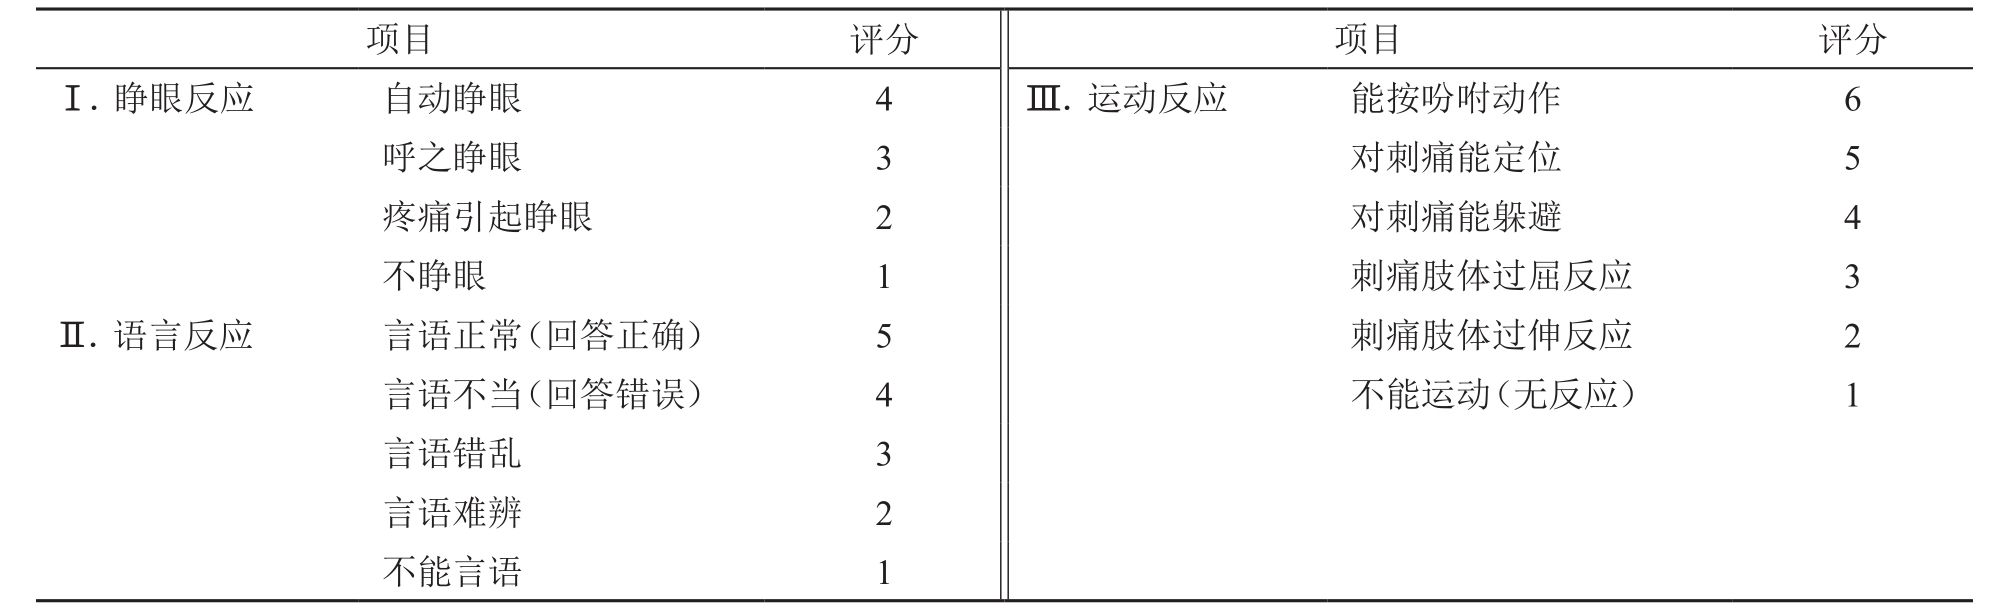
\includegraphics[width=6.66667in,height=2.03125in]{./images/Image00006.jpg}
\end{table}

\begin{table}[htbp]
\centering
\caption{Glasgow-Pittsburgh昏迷观察表}
\label{tab2-4}
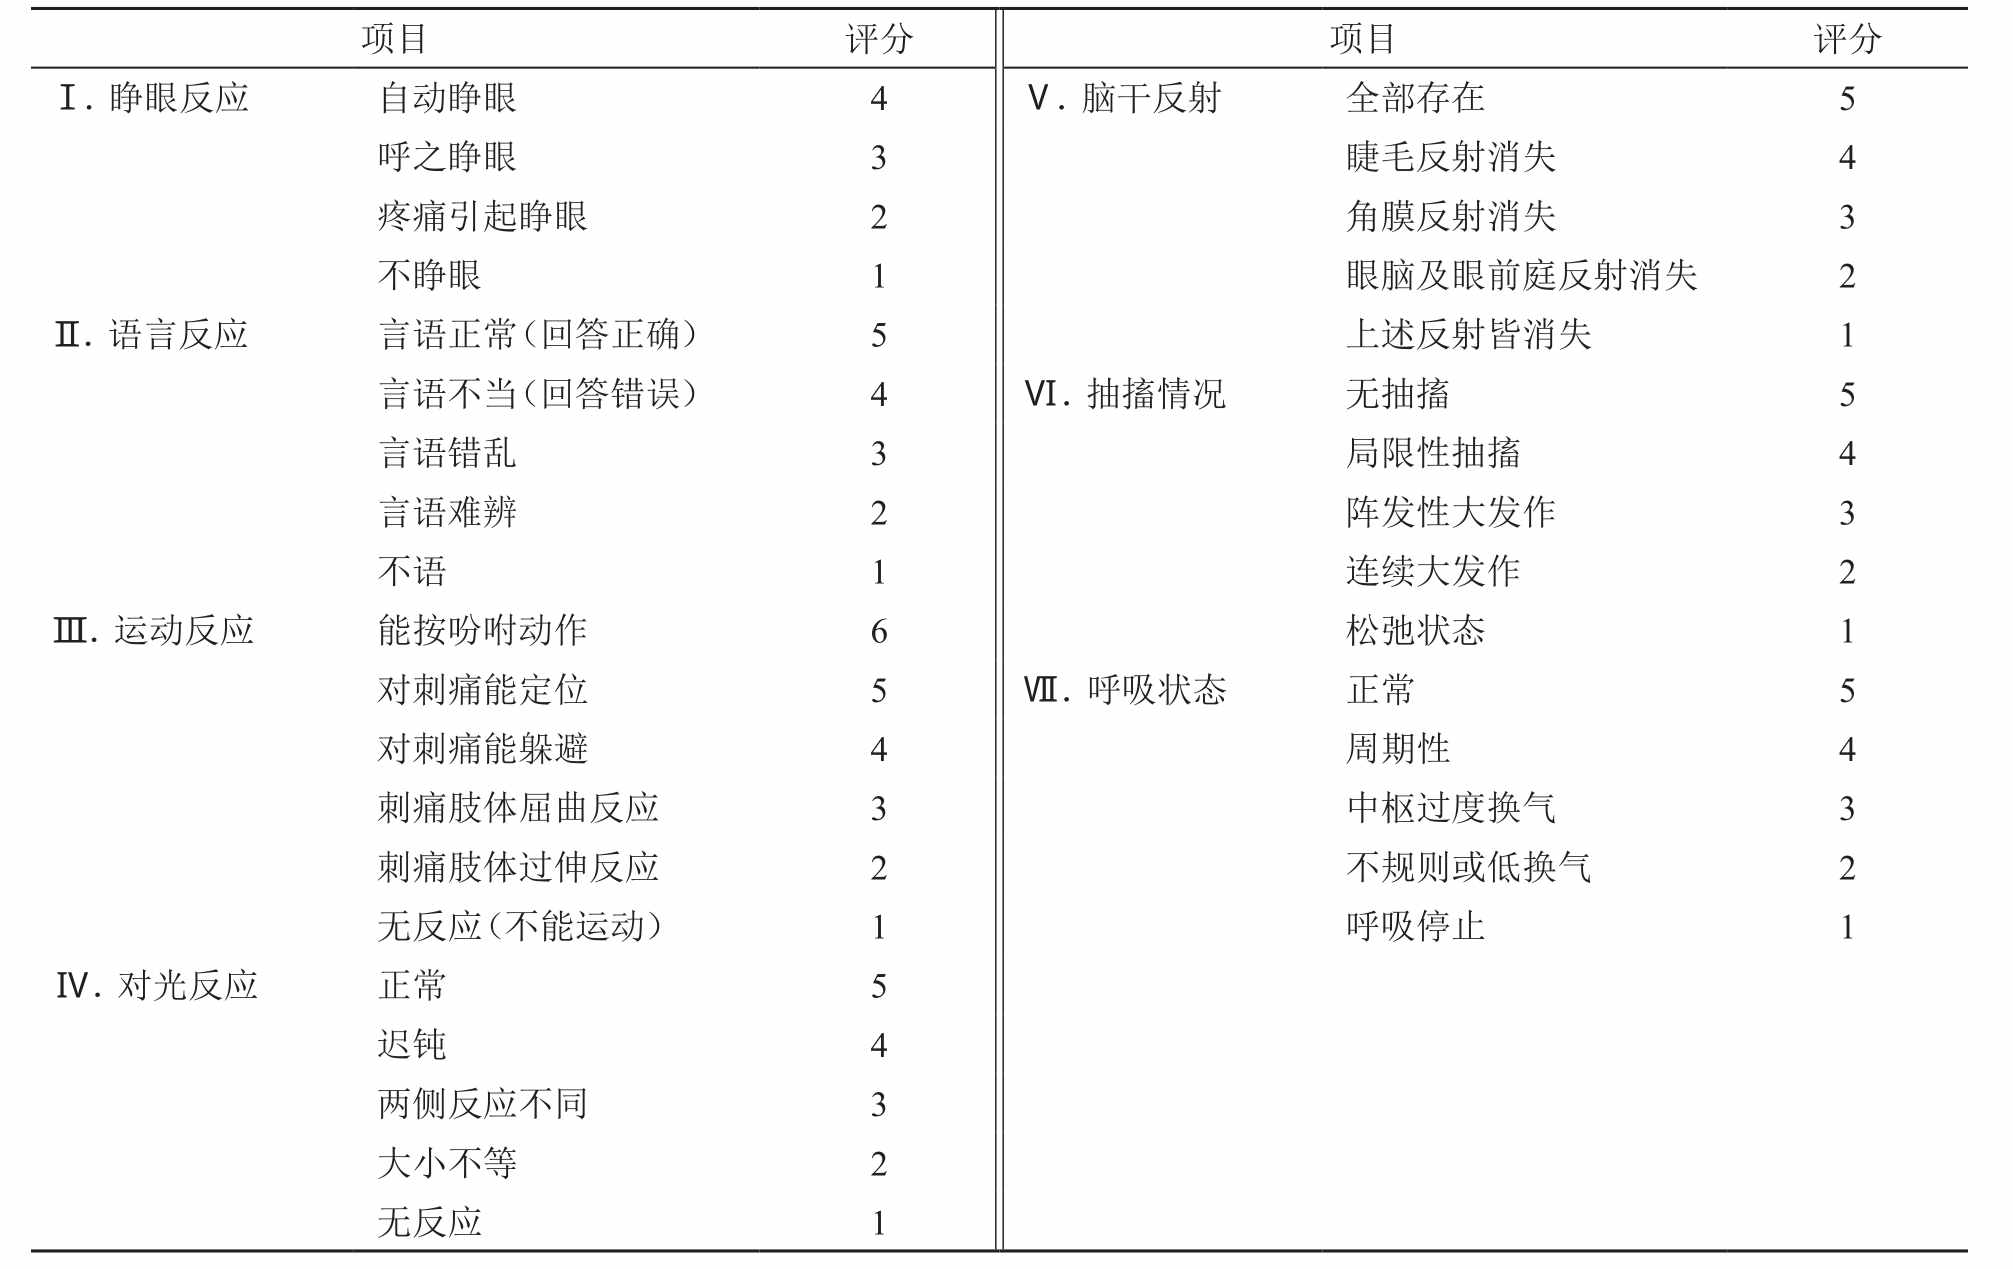
\includegraphics[width=6.69792in,height=4.21875in]{./images/Image00007.jpg}
\end{table}

如确定昏迷是颅内病变引起,尚可将颅内病变又进一步区分为颅内幕上局限性病变、幕下局限性病变和颅内弥散性病变三组。它们的特征参见表\ref{tab2-1}。

\paragraph{全身性疾病}

全身性疾病可影响脑代谢而引起弥散性脑损害,又称代谢性脑病。同原发性颅内病变相比,其临床特点为:先有颅外器官原发病的症状和体征,以及相应的实验室检查阳性发现,后才出现脑部受损的征象。由于脑部损害为非特异性或仅是弥散性功能抑制,临床上一般无持久性和明显的局限性神经体征和脑膜刺激征,主要是多灶性神经功能缺乏的症状和体征,且大都较对称;通常先有精神异常,意识内容减少。一般是注意力减退,记忆和定向障碍,计算和判断力降低,尚有错觉、幻觉,随病程进展,意识障碍加深。此后有的可出现不同层次结构损害的神经体征,如昏迷较深和代谢性呼吸抑制很严重,而眼球运动和瞳孔受累却相对较轻。脑脊液改变不显著,颅脑CT扫描等检查无特殊改变,不能发现定位病灶。其病因很多,它们的特征参见表\ref{tab2-2}。

\hypertarget{text00010.htmlux5cux23CHP1-2-2-4-2}{}
(二) 根据患者是否伴有脑膜刺激征和脑局灶体征来判断昏迷的病因

\paragraph{脑膜刺激征(+)而脑局灶性体征(−)}

\hypertarget{text00010.htmlux5cux23CHP1-2-2-4-2-1-1}{}
(1) 突发剧烈头痛:

蛛网膜下腔出血(脑动脉瘤、脑动静脉畸形破裂)。

\hypertarget{text00010.htmlux5cux23CHP1-2-2-4-2-1-2}{}
(2) 急性发病、发热在先:

化脓性脑膜炎、乙型脑炎、其他急性脑炎等。

\hypertarget{text00010.htmlux5cux23CHP1-2-2-4-2-1-3}{}
(3) 亚急性或慢性发病:

真菌性、结核性、癌性脑膜炎。

\paragraph{脑膜刺激征(−)而脑局灶性体征(+)}

\hypertarget{text00010.htmlux5cux23CHP1-2-2-4-2-2-1}{}
(1) 突然起病者:

如脑出血、脑栓塞、脑梗死等。

\hypertarget{text00010.htmlux5cux23CHP1-2-2-4-2-2-2}{}
(2) 以发热为前驱症状:

如脑脓肿、血栓性静脉炎、各种脑炎、急性播散性脑脊髓炎、急性出血性白质脑病等。

\hypertarget{text00010.htmlux5cux23CHP1-2-2-4-2-2-3}{}
(3) 与外伤有关:

如脑挫伤、硬膜外血肿、硬膜下血肿等。

\hypertarget{text00010.htmlux5cux23CHP1-2-2-4-2-2-4}{}
(4) 缓慢起病、颅内压增高者:

脑肿瘤、慢性硬膜下血肿、脑寄生虫病等。

\paragraph{脑膜刺激征(−)和脑局灶性体征(−)}

\hypertarget{text00010.htmlux5cux23CHP1-2-2-4-2-3-1}{}
(1) 有明确中毒原因:

如酒精、麻醉药、安眠药、一氧化碳中毒等。

\hypertarget{text00010.htmlux5cux23CHP1-2-2-4-2-3-2}{}
(2) 尿检异常:

尿毒症、糖尿病、急性尿卟啉症等。

\hypertarget{text00010.htmlux5cux23CHP1-2-2-4-2-3-3}{}
(3) 休克状态:

低血糖、心肌梗死、肺栓塞、大出血等。

\hypertarget{text00010.htmlux5cux23CHP1-2-2-4-2-3-4}{}
(4) 有黄疸:

肝性脑病等。

\hypertarget{text00010.htmlux5cux23CHP1-2-2-4-2-3-5}{}
(5) 有发绀:

肺性脑病等。

\hypertarget{text00010.htmlux5cux23CHP1-2-2-4-2-3-6}{}
(6) 有高热:

重症感染、中暑、甲状腺危象等。

\hypertarget{text00010.htmlux5cux23CHP1-2-2-4-2-3-7}{}
(7) 体温过低:

休克、酒精中毒、黏液性水肿昏迷等。

\hypertarget{text00010.htmlux5cux23CHP1-2-2-4-2-3-8}{}
(8) 头部外伤:

脑震荡等。

\hypertarget{text00010.htmlux5cux23CHP1-2-2-4-2-3-9}{}
(9) 其他:

癫痫等。

\subsection{处理原则}

\paragraph{昏迷的最初处理}

常规措施有:①保持呼吸道通畅,氧疗,必要时气管插管或切开行人工呼吸。②维持循环功能,尽早开放静脉,建立输液通路(1~3个)。有休克应迅速扩充血容量,使用血管活性药物,尽快使收缩血压稳定在100mmHg左右。有心律失常者应予以纠正;有心肌收缩力减弱者应给予强心剂;心跳骤停时应立即行心肺复苏。③纳洛酮:常用剂量每次0.4~0.8mg,静脉注射或肌注,无反应可隔10~15分钟重复用药,直达预期效果;亦可用1.2~2.0mg加入250~500ml液体中静滴。

\paragraph{病因治疗}

针对病因采取及时果断措施是抢救成功的关键。若昏迷的病因已明确,则应迅速给予有效病因治疗。如由颅内占位性病变引起者,若条件许可应尽早作开颅手术,摘除肿瘤;细菌性脑膜脑炎引起者,应迅速给予大量而有效的抗生素治疗;因脑型疟疾而引起的昏迷,则可给盐酸奎宁0.5g置于5\%葡萄糖液250~500ml中静滴;由于低血糖引起者应立即给予高渗葡萄糖液;若为有机磷农药中毒所致者,应立即用胆碱酯酶复能剂和阿托品等特效解毒剂;糖尿病昏迷应予胰岛素治疗等。

\paragraph{对症支持疗法}

包括控制脑水肿、降低颅内压,维持水电解质平衡,镇静止痛,防治各种并发症(如急性心力衰竭、急性呼吸衰竭、消化道出血、急性肾功能衰竭、急性脑功能衰竭等)等,详见有关章节。

\protect\hypertarget{text00011.html}{}{}

\hypertarget{text00011.htmlux5cux23CHP1-2-4}{}
参 考 文 献

1. 张文武.急诊内科学.第2版.北京:人民卫生出版社,2007

2. 贾建平.神经病学.第6版.北京:人民卫生出版社,2008

3. Rowland LP. Merritt's Neurology. 11th ed. New York:Lippincott
Williams & Wilkins,2005

\protect\hypertarget{text00012.html}{}{}

\chapter{眩 晕}

眩晕是一主观症状,是机体对于空间关系的定向感觉障碍或平衡感觉障碍,是一种运动错觉,患者感外境或自身在旋转、移动或摇晃。在眩晕症状出现的同时,常伴有平衡失调、站立不稳、眼球震颤、指物偏向、恶心、呕吐、面色苍白、出汗及心率和血压的改变。

临床上可将眩晕分为前庭系统性眩晕(亦称真性眩晕)及非前庭系统性眩晕(亦称头晕)。前者由前庭神经系统病变(包括前庭末梢器、前庭神经及前庭的中枢连接)所引起,为真性眩晕,表现为有运动错觉的眩晕,例如自觉旋转、摇晃、移动感;后者常为头昏(头重脚轻、眼花、头脑昏昏沉沉、颅内在转动等诉说),但并无外境或自身旋转的运动觉,常由心血管系统疾病,全身中毒性、代谢性疾病,贫血,眼病等疾患所引起。

\subsection{病因与发病机制}

\subsubsection{病因分类}

眩晕的病因分类有多种方法,各家不甚统一,各有其优缺点。笔者认为根据神经系统疾病的诊断步骤先定位再定性的方法,较为实用,即根据病变的解剖部位及结合病因予以分类。现将常见的疾病列举如下:

\hypertarget{text00012.htmlux5cux23CHP1-3-1-1-1}{}
(一) 前庭系统性眩晕

包括前庭末梢感受器
、前庭神经、前庭诸核、内侧纵束、小脑、前庭皮质代表区之各种病损所产生的真性眩晕。

\paragraph{耳源性}

例如外耳道耵聍,急、慢性中耳炎,咽鼓管阻塞,鼓膜内陷,耳硬化症,迷路炎,慢性中耳炎内耳并发症(瘘管形成),梅尼埃病(Meniere
disease),运动病,良性位置性眩晕,迷路动脉血供障碍,内耳震荡等。

\paragraph{前庭神经病损}

前庭神经元炎、听神经鞘膜瘤、脑桥小角其他肿瘤、前庭神经炎、前庭神经外伤(岩锥骨折)或中毒性损害。

\paragraph{脑干病变}

脑桥、延髓的血管性和肿瘤性病变、脑干脑炎、多发性硬化、延髓空洞症、第四脑室肿瘤及囊肿。

\paragraph{小脑病变}

肿瘤、脓肿、出血及损伤。

\paragraph{大脑病变}

颞叶肿瘤或血管性病变,颞叶癫痫。

\paragraph{颈椎病变}

颈椎肥大性改变及颈椎间盘突出。

\hypertarget{text00012.htmlux5cux23CHP1-3-1-1-2}{}
(二) 非前庭系统性眩晕

1.眼性眩晕 如眼外肌麻痹、屈光不正、先天性视力障碍等。

2.心血管病变 如高血压、低血压、心律不齐、心力衰竭、大脑动脉硬化。

3.全身中毒性、代谢性、感染性疾病。

4.各种原因引起的贫血。

5.神经症。

\subsubsection{发病机制}

机体平衡的维持,定向功能的正常,是借视觉、本体觉(肌腱、关节中)及前庭平衡觉的协同作用而完成的,而后者对机体姿位平衡的维持更为重要。各种外界的刺激(信息),通过上述诸感受器如视觉、本体觉、前庭平衡觉传入至前庭核群、红核、网状结构、皮质下中枢、小脑等,不断反射性调节机体对各种姿位的平衡,各种加速度的反应,使机体在运动中与外界环境保持协调与平衡。神经冲动由皮质下中枢再向上传入大脑皮质,多数学者认为皮质平衡中枢在颞叶,Penfield为患者作脑部手术时,电刺激颞上回,引起“头晕”、“旋转”和“摇摆”感。应用电生理方法在动物实验中测定了前庭皮质投射区,罗猴的前庭皮质投射区位于第一体感区和第二体感区之间的中央后回,为Brodmann第2区稍后处。前庭的皮质投射似乎从感觉-运动皮质移向顶叶的联合皮质,皮质区接受两侧前庭投射。综上所述,皮质前庭代表区虽不甚确切,但一般认为在颞上回的后、上半部,颞顶交界处及岛叶的上部。丘脑后下腹核很可能为前庭传入的丘脑换元站。后下腹核位于后外侧腹核和后内侧腹核之间的底部。

前庭系统包括内耳迷路末梢感受器(半规管中的壶腹嵴、椭圆囊和球囊中的位觉斑),前庭神经、脑干中的前庭核群,小脑、内侧纵束、前庭脊髓束、前庭皮质代表区。三个半规管中的壶腹嵴,其感受器在半规管中内淋巴流动时接受角加速度的刺激,而椭圆囊、球囊的位觉斑则接受直线加速度、重力加速度的刺激,冲动沿着前庭神经传入中枢,反射性地调节机体平衡。在正常情况下,从前庭器官传入中枢的有关平衡觉的信息并不为人所感知,只是当前庭器官或其中枢连接受到较大刺激或病理性损害时,前庭感受的刺激(信息)与来自肌肉、关节的本体觉及视觉感受器的关于空间定向的冲动不一致时,于是产生眩晕,亦即运动错觉。由于前庭核通过内侧纵束与动眼神经核之间有密切的联系,因此当前庭感受器、前庭神经及前庭核群受到病理性刺激(或破坏)时常出现眼球震颤,这种前庭性眼球震颤的特点为眼球有一慢相与一快相交替的有规律的来回颤动。慢相系由前庭-动眼反射通路实现,偏向前庭兴奋性相对较低的一侧。快相则为皮质下中枢、脑干网状结构向相反方向调节眼球运动的现象。因快相容易观察,通常即以此代表眼震的方向,与眩晕的感觉方向一致。前庭诸核通过内侧纵束、前庭脊髓束及网状脊髓束、前庭→小脑→红核→脊髓等通路,与脊髓中的前角运动细胞相连接,所以前庭病变时或前庭器受到较大的刺激时,除出现眼震外还可出现躯体向一侧倾倒及肢体错定物位(指物偏向)等体征。前庭核还与脑干网状结构中的血管运动中枢、迷走神经核等连接,所以前庭器病变时在眩晕的同时常伴有恶心、呕吐、苍白、出汗甚至血压、呼吸、脉搏等改变。

\subsection{诊断思路}

眩晕是一主观症状,为了对眩晕病因作出正确的诊断与鉴别诊断,必须详询病史,细致的体格检查,必要的辅助检查,并应熟悉与了解常见引起眩晕疾病的特点。

\subsubsection{病史}

应详细了解眩晕的性质、程度、时间、诱发因素、伴随症状以及可能引起眩晕的有关病史(药物中毒、外伤史)及询问包括神经科、内科、耳鼻喉科的有关疾病。

\subsubsection{体格检查}

\paragraph{神经系统方面}

除一般的神经系统检查外,特别应注意有无自发性眼球震颤、共济失调、听力障碍及颅内压增高征。

\paragraph{内科方面}

应检查血压、心脏,有无高血压、低血压、心律不齐、心功能不全,有无贫血、全身感染、中毒、代谢紊乱等。

\paragraph{耳科方面}

应检查外耳道、鼓膜、中耳、鼻咽部,注意有无耵聍阻塞外耳道,有无表皮样瘤性中耳炎及耳硬化症。疑有迷路瘘管时应作瘘管试验。

\paragraph{听力学检查}

应用表、音叉试验法可以大致了解听力情况、听力障碍的性质(传导性、感音性)及程度,必要时作电测听检查,包括作短增量敏感指数(SISI)试验、复聪(recruitment)试验。

\paragraph{前庭功能检查}

包括自发性眼震、倾倒、指物偏向、变温(caloric)试验、旋转试验、直流电试验、位置试验、视动性眼震试验,必要时还需作眼震电图(ENG)检查。

\subsubsection{辅助检查}

可根据病情作必要的辅助检查,例如头颅X线摄片、乳突摄片、脑电图、经颅Doppler超声(TCD)检查、头颅CT扫描、头颅磁共振成像、疑为颈椎病者则需作颈椎摄片或颈椎CT扫描。疑有颅内炎症者需作腰穿检查脑脊液。

\subsubsection{前庭功能检查的临床意义}

前庭功能检查对于眩晕症的诊断有肯定的价值,有助于确定病损的部位,鉴别眩晕的性质。前庭系统性眩晕常有前庭功能异常,而非系统性眩晕则多数均无明显的前庭功能异常。前庭功能检查项目繁多,兹将这些检查的临床意义叙述如下。

\paragraph{自发性眼球震颤}

前庭系统性眩晕常伴有眼震,而非系统性眩晕一般均无自发性眼震。前庭周围性病变及前庭中枢性病变时所出现的自发性眼震的鉴别大致有如下几点:①前庭周围性:眼震常为一种方向,多为水平性,多呈突发性,伴有明显眩晕且与眼震程度一致,闭目后眩晕症状并不减轻,固视可使眼震减弱,眼震之快相通常为向病损的对侧。闭目时向前伸出的两个上肢偏向病损侧,躯体常向眼震的慢相倾倒。常伴有听力减退。眼震持续时间一般不超过3周。如梅尼埃病、急性迷路炎、急性前庭神经损伤等。②前庭中枢性:眼震方向不一,可为水平、旋转、垂直、斜向,持续时间较长。不一定伴有明显眩晕,眩晕与眼震程度不一致。过指和倾倒方向并不恒定,与眼震方向无肯定关系。可能无听力障碍。眼震常不能被固视抑制(减弱)。病变多数累及脑桥、延髓或小脑,因天幕上病变直接引起眼震者罕见。

至于眼源性眼震,其特点是眼震呈摆动性,尤其当眼球在正中位时,眼震呈对称钟摆样;眼球移向侧方时转为跳动样眼震,其快相向侧视方向;闭目时眼震消失;眼震持续时间长;不伴旋转性眩晕,若有诉“眩晕”,常觉为外境来回摆动或“眼花”,闭目后症状即消失,无听力障碍,无自发性倾倒。眼源性眼震可见于先天性白内障,先天性角膜云翳,白化病。眼震在幼小时即已存在,也偶然发生于成年后罹患的黄斑变性患者。

\paragraph{变温试验(caloric test)}

常用的方法是微量法或冷热交替法(Hall pike法)。其临床意义如下:

(1)
单侧功能减退或消失(半规管轻瘫或瘫痪)常指示该侧前庭器有病变。例如听神经瘤、梅尼埃病等。

(2)
一侧性前庭功能减退或消失并伴有持久的自发性眼球震颤,则病损已累及脑干或小脑。如脑桥小脑角占位性病变已侵犯及脑桥或小脑。

(3)
双侧性前庭功能减退:提示两侧前庭器(或前庭神经)病变,常见于中毒性病损(链霉素中毒)、感染性病损(前庭神经元炎或脑桥小脑角蛛网膜炎)。

(4)
变温试验反应消失而前庭直流电试验反应存在,提示病损位于前庭神经末梢器,例如迷路炎。

(5)
有自发性眼震及眩晕,但变温试验时诱发出的眩晕反应及迷走兴奋反应不明显,常提示病变位于颅后窝。

(6)
变温试验所诱发的眼震、眩晕、指物偏向,它们彼此在程度上、性质上有分离或不一致;诱发的眼震为反常性(眼震的性质错乱,如原应出现水平性眼震却出现垂直性)者或反向性(眼震与应出现的方向相反)者;变温试验时诱发的眼震只出现在慢相方向上的双眼偏斜而无明确的快相,均提示病变位于脑干。

(7)
前庭功能亢进:有两种情况:①单侧性亢进提示该侧前庭神经(前庭器)有刺激性病变存在,例如迷路炎的早期、梅尼埃病的初期;②双侧性亢进可能为神经症,是由于自主神经功能失调等因素所引起,亦可能由于颅内某些疾病使小脑对前庭的正常抑制作用减退、中枢前庭神经元兴奋性增高所引起,无定位价值。

(8)
用冷热交替法检查前庭功能,除可发现半规管功能是否正常、有无半规管麻痹(反应低下或消失),并可发现有无优势偏向。所谓优势偏向是指所诱发出的眼球震颤反应向一侧的眼震时程较向另一侧的眼震时程明显增大,例如以温水刺激右耳和以冷水刺激左耳均引起向右的眼球震颤。若这两个反应时程均大于使眼震向左的相应变温刺激反应时即称为向右的优势偏向。通常认为向一侧方向的眼震时程总和大于向对侧者的总和40秒以上者,即为有优势偏向。在椭圆囊及其与前庭神经核尾端部分连接的紧张性前庭机制发生病变时即可引起向对侧方向的优势偏向。但大脑颞叶后部病变时,有时亦可发现有朝向病侧的优势偏向。

\paragraph{位置试验}

眩晕患者,尤其是其眩晕症状的发生与头部处于某种特定位置有关者(此种眩晕可称位置性眩晕),作位置试验有一定的临床诊断价值。通过检查可以了解眩晕出现时是否同时伴有眼震,并可进一步鉴别此种位置性眩晕、位置性眼震系由前庭周围性病变抑或中枢性病变所引起。

位置性眩晕与位置性眼球震颤的检查方法:①嘱患者坐于检查桌上,观察其有无自发性眼震。②检查者立于患者的右侧,嘱患者头向右侧偏转45°,躯体亦向右侧轻度偏转,检查者用两手扶住患者的头部,然后嘱患者迅速躺下,头仍维持于向右侧偏转的位置。事先作为测试让患者躺下后头部超过检查台一端并悬垂于检查台沿之外。检查者始终用两手扶持其头部,以维持其头部向右侧偏转的位置,观察有无眩晕症状及眼球震颤。观察15秒如无眩晕症状及眼震出现,则让患者恢复原先坐位,亦观察15秒,注意有无眩晕与眼震。③重复以上检查,嘱头向左偏转45°,然后再躺下观察。如果在上述检查中出现眩晕或眼球震颤,则需要观察眼球震颤的详细情况,包括眼震出现的潜伏期、眼震持续时程、眼震的方向及类型,并了解眩晕的程度,观察自主神经反应情况。对于有位置性眩晕及位置性眼球震颤的病例尚需在短期内连续检查数次(4~5次),使其症状与体征重复出现,观察连续检查数次后有无疲劳、适应现象(即原有的位置性眩晕与位置性眼震因连续反复检查而渐减退及消失)。

周围型与中枢型位置性眩晕、眼震的鉴别见表\ref{tab3-1}。

\begin{table}[htbp]
\centering
\caption{周围型与中枢型位置性眩晕、眼震的鉴别}
\label{tab3-1}
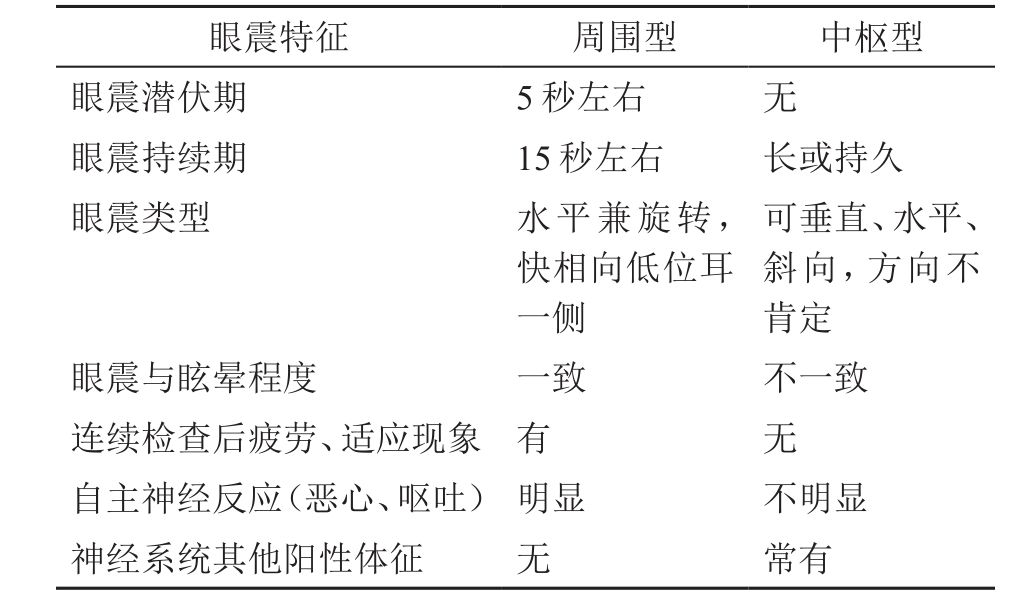
\includegraphics[width=3.36458in,height=2in]{./images/Image00008.jpg}
\end{table}

周围型位置性眩晕、眼震的常见疾病有良性阵发性位置性眩晕(即耳石病)、梅尼埃病、耳硬化症、内耳开窗术后、浆液性迷路炎、内听动脉供血不足、药物性内耳损害等。中枢性位置性眩晕、眼震的常见疾病可见于小脑蚓部肿瘤、第四脑室肿瘤或囊肿、椎-基底动脉供血不足、桥小脑角肿瘤、颅脑外伤等。

\paragraph{直流电试验}

应用直流电检查前庭神经,电流不仅刺激前庭末梢器,也能直接作用于前庭神经节及前庭神经。方法为将直流电负极置于测试耳的耳屏处或乳突处,正极置于前额或手中,电流逐渐缓慢增加,分别观察出现眩晕感、倾倒及眼震的毫安(mA)数,通常于正常人2~4mA即有眩晕感觉,4~6mA出现倾倒反应,6~8mA出现眼震。眼震之快相向负极侧,而倾倒则向负极之对侧。直流电试验主要的临床价值可协助鉴别前庭末梢器和前庭神经本身的病变。例如前庭末梢器病变(梅尼埃病、迷路炎)变温试验可能显示病侧前庭功能减退或功能消失,而直流电试验仍属正常反应。若病变累及前庭神经例如听神经瘤,则变温试验无反应时,直流电试验亦无反应。

\paragraph{视动性眼震试验(optokinetic test)}

视动性眼震由固视连续移动景物所引起而非前庭刺激所引起。试验原理:当两眼注视眼前连续而迅速通过的一系列物体时,每一物体在后一物体出现于视野中以前,受到两眼的注视与跟随。而当下一物体的影像落于视网膜的周边部时,眼球即反射性反跳,以便使后一物体像落于黄斑上。眼球如此快慢交替地运动,遂形成视动性眼球震颤,这是一种生理现象。此项检查之所以列入神经耳科学,是因为:①视动性眼震亦有快相与慢相的交替运动,与前庭性眼震形式类似;②此项检查对各种自发性眼震鉴别及颅内病变的定位诊断有一定价值。应用视鼓或视伞或带尺诱发眼球震颤。正常人所诱发之视动性眼震之慢相与视鼓旋转之方向一致,眼震之快相与视鼓旋转之方向相反,所诱发出之视动性眼震向左、右侧是对称的。

一般认为视动性眼球震颤的神经通路为:起自视网膜右半侧之神经纤维→右侧膝状体→视放射→视皮质(Brodman18区、角回和缘上回)的视动中枢,再自视动中枢通过视放射后部深处前行,离视放射→大脑脚→上丘→经内侧纵束→脑桥眼球同向运动中枢→眼球运动核。

因此,皮质视动中枢至脑桥同向运动中枢间任何部位之病变累及视动通路,即可消除或减弱向对侧之视动性眼球震颤,亦即出现向病侧之视动性眼震优势偏向。根据笔者研究的资料分析,在大脑半球占位性病变中,出现视动性眼震优势偏向现象多数与后颞、顶枕部(尤其是顶部)有关。如果病变累及脑干内的视动反射纤维,亦常有异常反应,多数为不对称性异常。在眼源性的自发性眼球震颤病例中,视动性眼震反应多数表现为同向性异常(即眼震的快相与视鼓或视伞旋转的方向相同),或无反应。

\paragraph{眼震电图(ENG)}

检查对于眩晕患者作前庭功能检查,其中自发性眼球震颤与诱发性眼球震颤都是检查中的一项重要体征,除肉眼观察外,应用眼震电图记录,可以使眼球震颤的各种特征(速度、频率、幅度、方向)客观记录下来,以供比较分析研究。通常所见到的节律型、水平性(或垂直性)眼震在眼震电图上表现为一不对称的峰形波,由迅速上升(或下降)的快相与缓慢回复至基线的慢相所组成。

眼震强度可用眼震时程、幅度、频率、慢相速度等表示,其中以时程和慢相速度为可靠。

慢相速度的测量方法如下:①正常眼震电图测量法:见图\ref{fig3-1}。②眼震强度------慢相速度计算法:其中几何作图法(图\ref{fig3-2})系延长慢相斜边成AC,使BC等于纸速1秒(s),若测得AB
= 22mm,定标值10°=
11mm,按速度=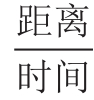
\includegraphics[width=0.30208in,height=0.32292in]{./images/Image00009.jpg}
,得

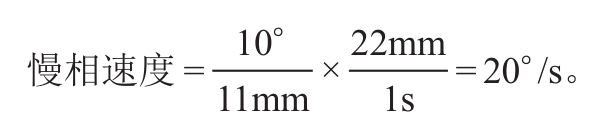
\includegraphics[width=1.95833in,height=0.42708in]{./images/Image00010.jpg}

\begin{figure}[!htbp]
 \centering
 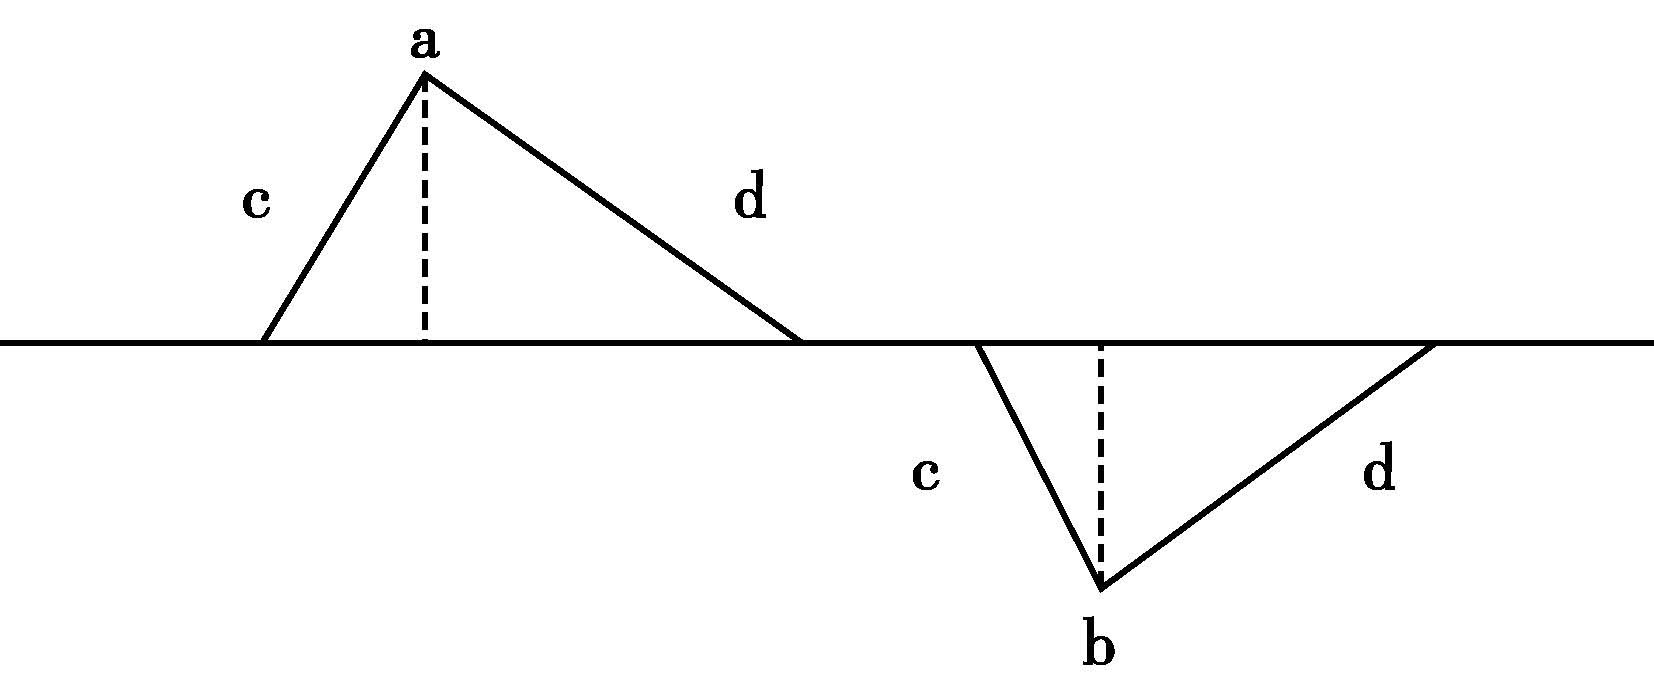
\includegraphics[width=2.75in,height=1.13542in]{./images/Image00011.jpg}
 \captionsetup{justification=centering}
 \caption{正常眼震电图}
 \label{fig3-1}
  \end{figure} 

a.右向眼震;b.左向眼震;c.快相;d.慢相

\begin{figure}[!htbp]
 \centering
 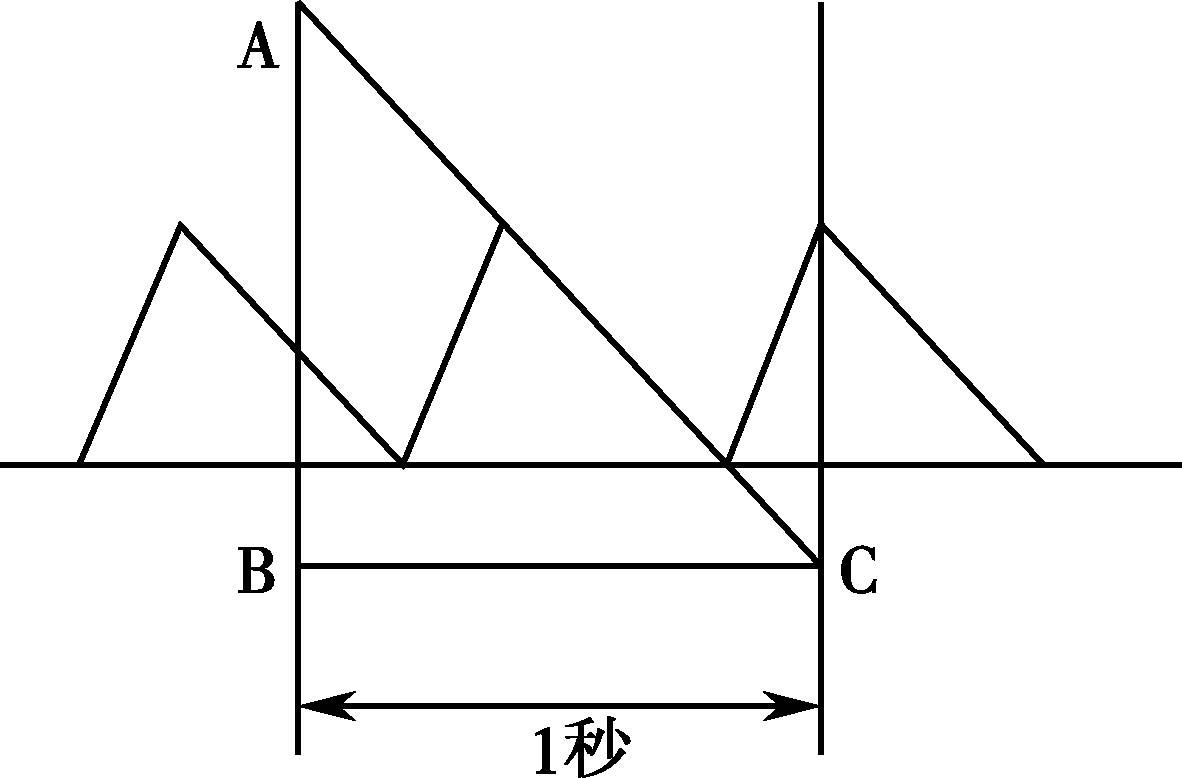
\includegraphics[width=1.96875in,height=1.29167in]{./images/Image00012.jpg}
 \captionsetup{justification=centering}
 \caption{几何作图法}
 \label{fig3-2}
  \end{figure} 

另为极盛期价值法(culmination
valve),于变温试验中,取反应高潮期10秒内之眼震,计算其幅度和频率,以慢相速度表示之。其公式如下:

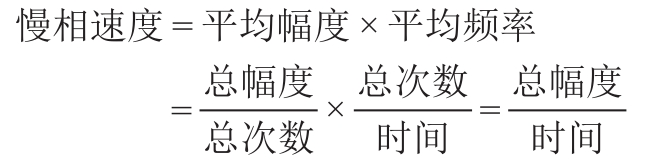
\includegraphics[width=2.16667in,height=0.53125in]{./images/Image00013.jpg}

例如:10秒内眼震总幅为150mm,总次数为20次,定标值10°= 11mm,则

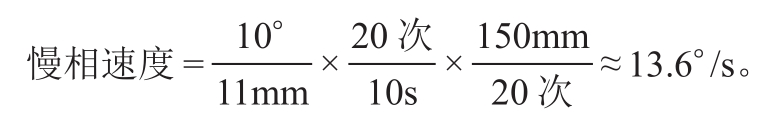
\includegraphics[width=2.57292in,height=0.40625in]{./images/Image00014.jpg}

利用眼震电图可以记录各种自发性眼震,并通过各种诱发试验记录变温性、位置性、视动性、凝视性眼球震颤。并可作扫视试验(saccade
test)、平稳跟踪试验(pursuit
test),于检查中可进一步观察在睁眼(明亮条件下)、暗室中、闭眼条件下眼震的变化。这些客观资料,均有助于对眩晕、眼震、前庭系统疾病的诊断。

\subsubsection{诊断注意事项}

对于临床医师而言,在对眩晕的病因作诊断与鉴别诊断时可先从以下几方面考虑:

1.前庭系统性眩晕抑或非系统性眩晕
一般而言,凡属前庭系统性眩晕均具有空间定向的感觉异常,具有运动错觉或运动幻觉的特点,或觉外境或觉自身在运动感(旋转、摇晃、向一侧移动);而非系统性眩晕则没有上述的特点,大多数患者对“眩晕”描述为头昏、头胀、头重脚轻、头脑内转动等。

2.前庭周围性眩晕抑或前庭中枢性眩晕
对于前庭系统性眩晕应进一步鉴别是前庭周围性病变还是前庭中枢性病变,两者的鉴别见表\ref{tab3-2}。

\begin{table}[htbp]
\centering
\caption{前庭周围性眩晕与前庭中枢性眩晕的鉴别}
\label{tab3-2}
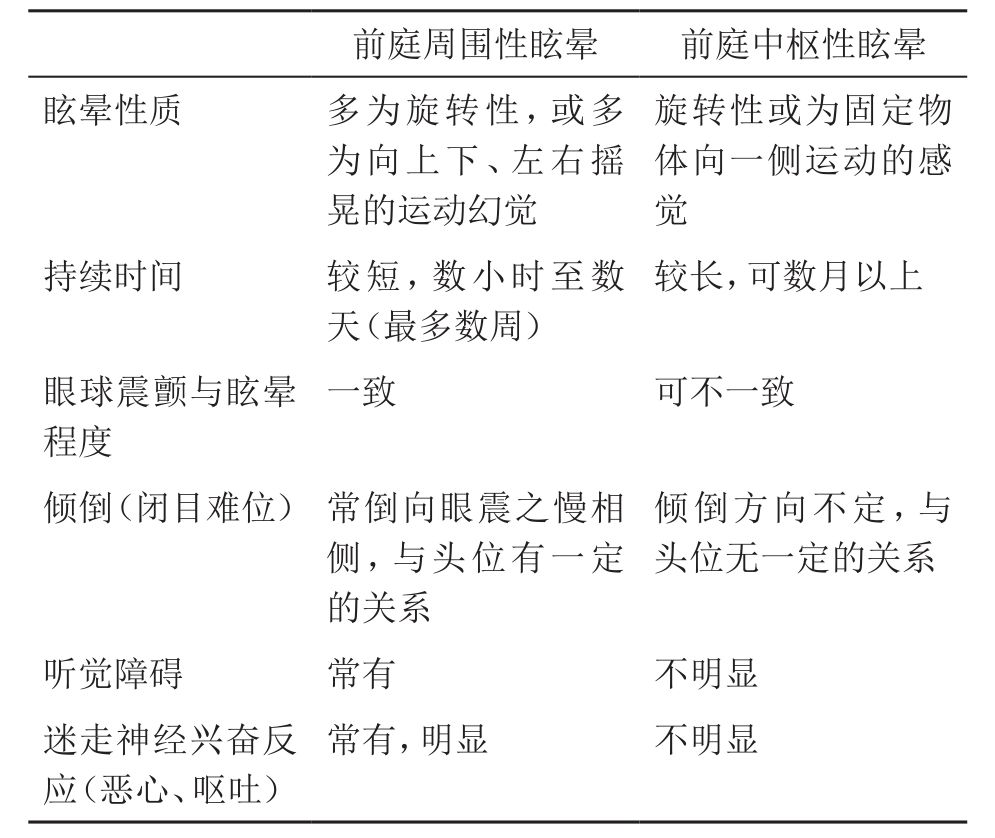
\includegraphics[width=3.3125in,height=2.78125in]{./images/Image00015.jpg}
\end{table}

3.更进一步的诊断需根据各疾病的临床表现的特点及必要的辅助检查。

\subsubsection{常见眩晕症疾患的临床特点}

\hypertarget{text00012.htmlux5cux23CHP1-3-2-6-1}{}
(一) 梅尼埃病(Ménière disease)

梅尼埃病系内耳病变,为中年以上阵发性眩晕的最常见的原因。临床表现为典型的三联症状:发作性眩晕,波动性、渐进性、感音性的听力减退和耳鸣。眩晕发作时常伴有恶心、呕吐、出汗、面色苍白、眼球震颤。眩晕常突然发作,发作前耳鸣增加,听力骤减,耳内有饱胀感。每次眩晕发作历时数小时至数天(多系1~2天)而自行缓解。发作间歇期长短不一,多数为数月一次,亦有一个月数次者。眩晕发作常常随耳聋的进展而减少,至完全耳聋时,迷路前庭功能消失,眩晕发作亦常终止。于眩晕发作间歇期间检查,仅可发现单侧(少数为双侧)感音性耳聋,作电测听检查部分患者重振试验(recruitment
test)呈阳性。前庭功能变温试验于一部分病例中显示功能减退。本病产生的原因可能是支配前庭器的交感神经功能失调引起迷路动脉痉挛,从而使内淋巴产生过多或吸收障碍,导致迷路水肿及内淋巴系压力增高,内淋巴腔扩大及内耳末梢器缺氧、变性等病理变化。

\hypertarget{text00012.htmlux5cux23CHP1-3-2-6-2}{}
(二) 良性发作性位置性眩晕(benign paroxysmal positional
vertigo,BPPV)

本病多见于中年以上患者,多数学者认为是耳石器病变所致,故又称此病为耳石病。患者常诉说当头部处于某一位置时即引起头晕,有些患者诉说半夜翻身时突然发生眩晕,若再回复该头位又即会再发生,因而患者尽可能回避该头位。眩晕严重时伴有恶心、呕吐。常无听力障碍。作头位位置检查,常能在患者所诉说的那个头位引起眩晕,同时可见有短暂的水平兼旋转性眼球震颤,眩晕与眼震一致,持续10~20秒自行缓解。重复该头位可重复出现眩晕与眼震。但于短期内连续数次重复检查,则可逐步适应而不出现眩晕症状与眼震。变温试验提示前庭功能正常。病程常为自限性,数周至几个月后可自愈。近年来一些学者研究认为其基本病理机制系椭圆囊斑上耳石脱落、游离的耳石进入后半规管并在内淋巴内移动,在头位变动时刺激后壶腹嵴,于是乃产生短时间的眩晕。至于耳石器病变的原因主要有:①前庭动脉前支血栓形成;②颅脑外伤致内耳震荡。在作头位位置试验时,重复数次检查后之所以出现适应(疲劳)现象是由于耳石散落在内淋巴腔,一时未能沉积在后壶腹顶部,故不再引起症状,但待耳石沉积在壶腹顶部时可再度诱发位置性眩晕与眼震。

\hypertarget{text00012.htmlux5cux23CHP1-3-2-6-3}{}
(三) 非良性位置性眩晕

颅后窝的占位性病变也可引起位置性眩晕
,这与上述良性位置性眩晕在临床表现上有以下区别:此种眩晕的发生往往在头位改变后立即出现,无潜伏期,诱发之眩晕持续时间较长,往往引起恶心、呕吐,眩晕可在数种头位诱发,而不像BPPV只在较特定的1~2种头位才诱发。常见的疾病是第四脑室、小脑蚓部的肿瘤或第四脑室的囊肿,亦可见于小脑半球、脑桥小脑角的肿瘤。除位置性眩晕外,有时有肢体或躯干的共济失调。

\hypertarget{text00012.htmlux5cux23CHP1-3-2-6-4}{}
(四) 前庭神经元炎(vestibular neuronitis)

起病较急,表现为突起的剧烈的眩晕,伴有恶心、呕吐,但无耳蜗症状。起病时常伴有感染(多为上呼吸道)症状,可能是一种病毒感染。发病时有自发性水平性眼球震颤,躯体平衡失调。变温试验显示病侧前庭功能减退或缺失,有时双侧均有损害。预后良好,一般在数周后眩晕症状逐日减轻,但变温试验示前庭功能呈永久性损害。多数学者认为病变主要为病毒侵犯前庭神经的Scarpa神经节,但也有少数学者认为有时脑干内的前庭纤维也受侵犯。

\hypertarget{text00012.htmlux5cux23CHP1-3-2-6-5}{}
(五) 迷路炎

单纯性中耳炎由于炎症刺激使迷路充血可引起眩晕。眩晕程度较轻,中耳炎好转后眩晕亦即解除。中耳炎并发弥漫性化脓性迷路炎时,眩晕严重,伴恶心、呕吐、眼震及病侧听力严重丧失,病侧前庭功能消失。此外还有耳痛、耳漏、头痛、发热等中耳感染症状与体征。慢性中耳炎侵蚀骨迷路有瘘管形成时,常有反复发作的眩晕。瘘管试验(以希格尔镜利用橡皮球增减外耳道压力,通过瘘管影响迷路,产生前庭反应)呈阳性反应。提示内耳有瘘管存在。

\hypertarget{text00012.htmlux5cux23CHP1-3-2-6-6}{}
(六) 药物性眩晕

在临床药物应用中
,有些药物因使用不当,因毒性作用而致眩晕,如链霉素;有些是难以避免的副作用,如某些镇静药和安眠药;有些是过敏所引起。

\paragraph{耳毒性抗生素类}

以氨基糖苷类为主,如链霉素(尤其是硫酸链霉素)、新霉素、卡那霉素、庆大霉素、阿米卡星(丁胺卡那霉素)等,其他尚有万古霉素、多黏菌素B。其中有些药物性损害主要影响前庭部分,但大多数前庭与耳蜗均有影响。链霉素是最常见者,引起眩晕症状通常于疗程第4周出现,但亦有仅应用4天即有眩晕症状者。在年老患者或有肾功能不全的患者,更易出现毒性作用。眩晕症状持续,而在患者行走、头部转动或转身时症状更为明显。于静止时、头部不动时,上述症状明显好转,甚至消失。而一旦活动后上述症状又复出现。前庭功能检查,大多数患者均无自发性眼球震颤,闭目难立征阳性,向左右前后摇晃方向不定。变温试验示双侧前庭功能均明显减退或消失。如伴有耳蜗损害,则尚有双侧感音性耳聋。眩晕症状消失较为缓慢,需数月甚或1~2年之久,前庭功能则更难恢复。

\paragraph{麻醉 、镇静和催眠药}

这类药物引起眩晕的机制主要是对中枢的抑制作用,皮质中枢受抑制时表现为头晕及轻度失平衡,并无明确的运动错觉。于麻醉后,由于皮质中枢的强抑制,有关平衡的各种传入信息,不能在中枢获得综合与分析,因而出现头晕症状,患者诉说昏昏沉沉。这些药物中除麻醉药外还有异丙嗪(非那更)、苯巴比妥(鲁米那)、利眠宁(氯氮{}
)等。

\paragraph{抗癫痫药}

在抗癫痫药中苯妥英钠与扑米酮是引起眩晕的最常见者,尤其是苯妥英钠,因应用广,应用时间又长,如不注意服用剂量及检测药物血药浓度,则甚易引起中毒性损害。主要损害于前庭末梢器,可累及小脑,均可导致眩晕,平衡失调,眼球震颤,共济失调,因此对于这些患者应定期随访,必要时检测药物血药浓度,调整药物剂量。扑米酮能用于抗痫治疗,虽较少用,但初服此药时,其剂量应减少至甚小量(成人常规用量之1/3~1/4),然后缓慢增加,才可避免眩晕。

\paragraph{其他药物}

如水杨酸类(水杨酸钠)、噻嗪类利尿剂(氢氯噻嗪)、降压药(利血平、降压灵)及某些磺胺类药均可致眩晕,在临床应用时应予注意。

\hypertarget{text00012.htmlux5cux23CHP1-3-2-6-7}{}
(七) 血管性眩晕(椎-基底动脉血循环障碍)

\paragraph{迷路卒中}

由于动脉粥样硬化或伴有血液黏稠度增加,血压的偏低,导致内听动脉血栓形成,常产生急骤的、严重的眩晕,伴恶心、呕吐,若耳蜗分支同时受损,则伴有耳聋及耳鸣。患者年龄较大,起病甚快,有身体其他部位动脉硬化的征象,既往(青、中年时)无类似的眩晕发作史等特点,均有助于与其他急性眩晕相鉴别。但有的患者表现短暂性的眩晕发作,伴有或不伴有耳蜗症状,持续数分钟至数小时即缓解,对于这些中、老年患者,若除外耳源性眩晕的其他疾病,可诊断为迷路动脉短暂性缺血发作(TIA)。

\paragraph{小脑后下动脉血栓形成}

亦称延髓外侧综合征(Wallenberg
syndrome)。其典型的症状与体征包括突起眩晕,伴恶心、呕吐,眼球震颤;病侧肢体共济失调及颈交感神经麻痹综合征;吞咽困难及同侧软腭麻痹、声带麻痹;病侧面部及对侧躯体、肢体的痛温觉减退或消失。

\paragraph{椎-基底动脉供血不足(vertebrobasilar insufficiency,VBI)}

多数表现为椎-基底动脉的TIA,临床常见。有关本病的概念至今还不十分清楚。引起VBI的病例基础是:①椎动脉的解剖特点:起始于两侧锁骨下动脉之椎动脉,需穿过第6~1颈椎横突孔后再经枕大孔入路,然后合并为基底动脉,椎动脉在行程中需经过一条活动度较大的骨性隧道。②椎动脉易发生动脉粥样硬化,随着年龄增大其动脉管径逐渐变窄,血流量亦渐变少。③中年以后颈椎常发生退行性变及骨赘形成。因此椎动脉的血流易受到各种因素的影响,例如颈部的转动,血压的较快的降低,血管的痉挛,血黏度的增高。因此VBI的发病通常认为主要是动力学改变所致,但也有部分患者VBI是由于循环系统内的微栓子所造成。由于迷路、前庭神经核、小脑的血液供应均来源于椎-基底动脉血流循环,因此VBI的主要临床表现是眩晕,常突然发生,颈部过度伸屈或旋转有时可诱发,眩晕发作持续通常短暂,常常数分钟即缓解,但可在短时期内反复发生多次,眩晕发作时可伴有恶心、呕吐、站立不稳,亦可伴有椎-基底动脉的其他供应区缺血的临床征象,例如视幻觉、偏盲、猝倒发作、复视、面麻木、进食吞咽困难,肢体肌力减退或感觉障碍,共济失调。上述这些临床表现通常都是呈发作性、短暂性,症状持续数分钟至数小时,不超过24小时,这一类型的VBI可称之为VBTIA(椎-基底动脉短暂性缺血性发作),但临床上也有一部分患者表现为在一段时期内(数天至数周)经常性的头晕,行走不稳,在除外了其他引起眩晕的疾病后亦应考虑为VBI,推究其发病机制是后循环的动力学障碍所致,应予重视。

对于VBI的诊断应根据具体情况选择作下列检查:①颈椎X线片,包括正、侧及斜位片,以发现有无颈椎病及其严重程度及了解有无骨刺可能累及椎动脉。②颈椎CT或颈椎MRI或螺旋CT,以进一步了解颈椎骨骼及脊髓和有关椎动脉受压、变窄情况。③头颅MRA,以了解颅内血管情况,尤其是了解椎-基底动脉及颅内脑底动脉环情况。④TCD检查。⑤BAEP检查。⑥SPECT检查。上述三项检查在VBI的病例中均有相当的阳性率,可作为诊断的参考依据。⑦前庭功能检查主要是作变温试验,对于了解前庭功能有肯定的价值。⑧眼震电图检查:可作扫视试验、凝视试验、跟踪试验、视动试验。有一定的临床价值。

关于椎-基底动脉短暂性缺血性发作的诊断依据:①中老年患者(发病在50岁以上)。②发作性眩晕,每次持续时间短暂,通常为数分钟至数十分钟。③眩晕发作时可伴有一种或数种脑干、小脑、枕叶的缺血症状及体征。④临床症状除轻度眩晕,行走不稳外均在24小时内减轻以至消失。⑤实验室检查(上已述及)有两项以上的阳性发现。⑥排除引起眩晕的其他病因。

\paragraph{颈椎病变}

颈椎退行性病变导致椎间隙狭窄,及由于钩椎关节骨赘增生刺激或压迫椎动脉,使椎动脉痉挛、阻塞,当转颈时一侧之椎动脉更易受压。若椎动脉本身已有粥样硬化,一侧椎动脉受压后,对侧椎动脉无法代偿则出现症状。临床常见之症状为发作性眩晕,其发病与头颈转动有密切关系。此外,这些患者尚可伴有枕部头痛、猝倒、视觉症状(闪光、视野缺失)及上肢麻痛。颈椎X线片、颈CT扫描可显示颈椎形态学病变改变。

\hypertarget{text00012.htmlux5cux23CHP1-3-2-6-8}{}
(八) 颅内肿瘤

由于颅内肿瘤所产生的眩晕有两种机制
:一是由于肿瘤直接压迫、浸润前庭神经或其中枢连接;另一是由于颅内压增高,尤其是由于肿瘤阻塞脑脊液循环而产生脑积水,引起第四脑室底部前庭核的充血和水肿。

\paragraph{桥小脑角肿瘤}

特别是听神经瘤,有轻度眩晕和耳鸣、耳聋,这是听神经瘤的早期症状。病变进一步发展可出现邻近脑神经受损的体征,如病侧角膜反射减退、面部麻木及感觉减退,展神经麻痹、周围性面瘫、眼球震颤,同侧肢体共济失调。在听神经瘤的早期通常并没有自发性眼球震颤,当肿瘤增大压迫脑干或小脑时才会出现,但一经出现则持续存在。听神经瘤至病程后期还可出现颅内压增高症状,头痛、视神经乳头水肿。对于听神经瘤的早期诊断可根据单侧性听力渐进性减退、听力检查为感音性耳聋;同侧前庭功能早期即消失,邻近脑神经(三叉、展、面神经)中有一根受累即应考虑为听神经瘤。若脑脊液中蛋白质含量增加,X线片上示病侧内听道扩大诊断即可肯定。近年来由于应用头颅CT及MRI检查,更易得到早期确诊。

\paragraph{脑干}

(延髓脑桥)肿瘤
因病变累及前庭神经核,常有眩晕及持久的眼震,可有一侧或双侧听力减退,水平性眼震的方向通常为双向性,向左侧注视时快相向左,向右侧注视则快相向右,也可能兼有旋转性眼震。当眼震明显时,眩晕症状不一定很重。还可以有其他脑神经障碍(主要为第Ⅴ、Ⅵ、Ⅶ、Ⅹ、Ⅺ)及对侧肢体瘫痪。

\paragraph{小脑半球肿瘤}

常有眩晕,早期即出现明显的振幅粗大的眼球震颤,及病侧肢体共济失调,水平性眼震的方向通常是两侧性的,但主要是向病变一侧。前庭功能变温试验示病侧肢体偏斜反应不明显。

\paragraph{小脑蚓部肿瘤及第四脑室肿瘤(或囊肿)}

眩晕为常见症状,眩晕的发生或加重常与头位位置有关。作头部位置试验,可见有中枢型位置性眼球震颤,并有早期颅内压增高及固定头位等临床表现。

\paragraph{天幕上肿瘤}

通常并不出现眩晕,如有则可能与颅内压力增高有关,但颞叶肿瘤有时可出现以眩晕为主要表现的癫痫样发作。脑电图上可以有痫样发放。

\hypertarget{text00012.htmlux5cux23CHP1-3-2-6-9}{}
(九) 外伤性眩晕

颅脑外伤时可因内耳迷路
、第Ⅷ脑神经、中枢前庭核及其中枢连接受损而产生眩晕。这些结构可单独或合并受损。迷路内外伤性出血的患者有周围型的前庭紊乱症状,常有颞骨骨折及听力同时受损的征象。亦有内耳并无出血而为迷路震荡者,则眩晕症状持续时间短、恢复较快,听力障碍程度亦较轻。部分患者可由于耳石器损伤而出现短期的位置性眩晕。颞骨横行骨折,骨折线横断岩锥,可产生听神经直接受损,出现明显的眩晕、自发性眼震、听力丧失,于4~6周内前庭症状逐渐消失,但听力常难以恢复。

严重的颅脑损伤患者,在第四脑室及导水管周围可见有点状的少量出血,损伤涉及前庭核及其中枢连接。脑干损伤后产生眩晕的同时常伴有脑干损伤的其他体征,如复视、面瘫、瞳孔不等大、肢体运动或感觉障碍等。眩晕症状持续较久,可达数月以上。颈部鞭索样损伤后亦常有眩晕症状,在头部运动时,尤其是向着颈部鞭索样受损的方向运动时,眩晕症状更易出现。每次眩晕发作数秒至数分钟。头位位置试验可有位置性眼震,常发生于头部转向鞭索样损伤侧,可能是由于内耳耳石器受损所致。

\hypertarget{text00012.htmlux5cux23CHP1-3-2-6-10}{}
(十) 精神性眩晕

精神性眩晕在本质上是神经症的一种表现。大多感觉头昏脑胀,非真性眩晕,无运动错觉,患者诉“眩晕”、“头晕”时无自发性眼震或自发性倾倒,往往常有神经症其他表现如失眠、焦虑、紧张、记忆力减退、注意力难集中等。无前庭系或非前庭系器官性疾病。起病诱因系以情绪、精神因素为主。

\subsection{处理原则}

\subsubsection{一般处理}

对于急性眩晕发作的患者,需卧床休息,饮食以流质为宜。伴有明显恶心、呕吐者,应酌情给予静脉补液,以维持营养,并需注意水、电解质的平衡。对于焦虑紧张的患者,应给予适当的病情解释与安慰,以解除顾虑。眩晕发作缓解后,应鼓励患者早日逐渐参加日常活动,适应日常生活。

\subsubsection{病因治疗}

因中耳炎并发症引起的急性化脓性迷路炎,应由耳科作必要的手术及抗感染治疗。由颅内占位性病变如小脑肿瘤、听神经瘤引起者,需作手术摘除肿瘤。由于梅尼埃病产生的眩晕,主张调节自主神经功能,平时以低盐饮食为宜。对于由药物中毒性损害引起的眩晕患者,应及时停药,并给予维生素B族药物。因颈椎骨质增生、椎间盘膨隆或突出而致的眩晕,可先作颈椎牵引或作颈托固定。必要时再考虑手术治疗。因心律失常或血压过高、偏低者,则需给予相应的内科治疗。因贫血引起的眩晕应纠正贫血。凡此种种的有关病因的处理均属重要,不可忽视。

\subsubsection{对症处理}

在病因治疗的同时,对于眩晕症状需给予药物治疗,以减轻眩晕症状及减少伴发的恶心、呕吐、焦虑、紧张等症状。

\paragraph{急性发作期的药物治疗}

可考虑选用的药物有:氢溴酸东莨菪碱0.3mg,肌肉注射;茶苯海明(晕海宁,dramamine)50mg,肌肉注射;硫酸阿托品0.5~1mg,肌肉注射;山莨菪碱(654-2)5~10mg,肌肉注射;盐酸异丙嗪(非那更)25~50mg,肌肉注射。以上药物可选择应用,并可根据病情每隔4~6小时重复给药2~3次。

\paragraph{眩晕发作后尚有轻度症状或慢性眩晕的治疗}

在急性眩晕发作后,虽已无明显的旋转幻觉,但仍有平衡失调、站立不稳的感觉,或在头部、身体转动时有这些症状,或眩晕程度虽轻但经常存在者,可选用各种镇静剂、安定剂,例如苯巴比妥0.015~0.03g,或地西泮(安定)2.5~5mg,或氯丙嗪25mg等,均为每天2~3次,口服。

\paragraph{几种治疗眩晕症的常用药物}

\hypertarget{text00012.htmlux5cux23CHP1-3-3-3-3-1}{}
(1) 镇静剂与安定剂:

例如苯巴比妥、溴剂、地西泮等。它们的药理作用对于前庭反应有抑制作用,对于一般感觉亦起抑制作用,因此可以减轻眩晕症状,消除紧张、烦躁不安、焦虑等症状。苯巴比妥虽可以减轻眩晕,但也常有全身抑制的作用,如疲倦、乏力。地西泮能减轻眩晕症状,减少紧张、焦虑,并有止吐作用,但可加强其他中枢抑制剂的作用。大剂量的安定类药物可以引起锥体外系的副作用。

\hypertarget{text00012.htmlux5cux23CHP1-3-3-3-3-2}{}
(2) 抗组胺药物:

例如苯海拉明、盐酸异丙嗪、氯苯那敏、盐酸氯苯苄嗪(敏克静)、茶苯海明等,这些药物用于治疗眩晕,其治疗效应可能是由于它们药理上的镇静作用而不是抗组胺作用。它们应用于眩晕发作期尚有止吐作用。

\hypertarget{text00012.htmlux5cux23CHP1-3-3-3-3-3}{}
(3) 止吐剂:

常用者为盐酸氯苯苄嗪及异丙嗪,均有明显止吐作用,适用于运动病及眩晕时伴有明显的自主神经反应(恶心、呕吐)的病例。这些药物亦有镇静作用及抗组胺作用。

\hypertarget{text00012.htmlux5cux23CHP1-3-3-3-3-4}{}
(4) 抗胆碱药物:

常用药物系东莨菪碱与阿托品,对于梅尼埃病的治疗效果较好。这类药物尚有止吐及解除血管痉挛的作用。东莨菪碱还有镇静作用,可优选使用。

\hypertarget{text00012.htmlux5cux23CHP1-3-3-3-3-5}{}
(5) 血管舒张药物:

例如烟酸、妥拉唑啉、山莨菪碱、地巴唑,这些药物并不是前庭抑制药物,其药理作用为解除血管痉挛。可应用于因血管痉挛、缺血性病变所引起的眩晕,如梅尼埃病的发作期及椎-基底动脉供血不足的病例。此外倍他司汀(betahistine,抗眩啶)亦有扩张血管的作用,常用量为4mg,每日3次;甲磺酸倍他司汀(敏斯朗)亦有类似的作用,6mg,每日3次口服。

\hypertarget{text00012.htmlux5cux23CHP1-3-3-3-3-6}{}
(6) 钙拮抗剂:

目前常用者有尼莫地平20mg,每天3次;桂利嗪(脑益嗪)25mg;每天3次,氟桂利嗪(flunarizine,商品名西比灵)5mg,每天1~2次,均为口服。

\hypertarget{text00012.htmlux5cux23CHP1-3-3-3-3-7}{}
(7) 增强动脉血氧分压和血氧饱和度药物:

阿米三嗪萝巴新{[}都可喜(Duxil){]}内含阿米三嗪和萝巴新,本药可增迷路和脑组织的血氧供应,对于因缺血缺氧而产生的眩晕疾患有较好的疗效,常用量为30mg,每天2次,口服。


\hypertarget{text00013.htmlux5cux23CHP1-3-4}{}
参 考 文 献

1. 史玉泉.实用神经病学.第3版.上海:上海科学技术出版社,2004

2. Norre ME. Clinical value of caloric test. Clin
Otolaryngol,1988,13:247

\protect\hypertarget{text00014.html}{}{}

\chapter{晕 厥}

晕厥(syncope)又称昏厥,是由于短暂的全脑组织灌注降低而导致的一过性意识丧失(transient
loss of
consciousness,TLOC),以快速发作、持续时间短和自限性为特点。可因血管迷走反射、直立性低血压、心输出量减少引起全脑低灌注,或由于脑干椎-基底动脉缺血引起脑干选择性低灌注所致。晕厥发作起病突然,持续时间短,典型可分为三期,其基本临床特点为:①发作前期:患者常感头部及全身不适、头晕、视力模糊、耳鸣、面色苍白、出汗,预示即将发生晕厥;此时患者如取头低位躺卧姿势常可防止发作。②发作期:轻者眩晕、恶心、躯体发软,眼前发黑,重者常突然意识丧失,全身肌紧张度消失,跌倒地上。意识丧失超过15~20秒可发生阵挛动作,有时有呼吸暂停,心率减慢,甚至心脏暂停搏动,瞳孔散大,流涎,尿失禁等;其特点是发作时间短暂,一般持续1~2分钟左右。脑电图检查可见持续3~10秒的广泛性、对称性2~3Hz的慢波。③发作后期(恢复期):患者平卧后意识迅速恢复(数秒至数分钟),可遗留紧张、头晕、头痛、恶心、苍白、出汗、无力和便意感等,甚至呕吐及括约肌失禁。休息数分或数十分钟缓解,不留后遗症,偶有极短暂的(<
30秒)发作后模糊状态伴定向力障碍和易激惹。

可见晕厥的特征是:发作突然,意识丧失时间短,不能维持正常姿势或倒地,在短时间内迅速恢复,罕有后遗症。

当前急诊对晕厥的评估已经从诊断晕厥的病因转变为进行危险分层,其目的是:①识别有威胁生命的疾病并收入院;②识别低危患者,可以让他们离院,并且以后到专科就诊;③识别不需要进一步诊断和治疗的患者;④对初步评估不能得出结论的患者进行进一步检查。

\subsection{病因与发病机制}

引起晕厥的病因很多(表\ref{tab4-1}),但任何原因均是通过影响脑血流,引起脑血供障碍所致。人脑重量占体重的2\%,而脑耗氧量却占全身耗氧量的20\%。脑组织几乎无氧和葡萄糖储备,全靠血循环提供外源性补给才能维持其正常的生理功能。健康成人的脑血流量为每100g脑组织45~50ml/分钟,而维持人的意识水平所需最低限度的脑血流量(即临界值)为每100g脑组织30ml/分钟,当脑血流量骤减至此临界值则可发生晕厥。

\paragraph{反射性晕厥(神经介导的晕厥)}

此类晕厥主要由于在正常状态下控制循环系统的心血管反射对刺激因素出现间歇性的不恰当反应,引起血管扩张和(或)心动过缓,导致动脉血压降低及全脑灌注减少。依据诱发因素不同又可分为以下几类:

\begin{table}[htbp]
\centering
\caption{晕厥的病因分类}
\label{tab4-1}
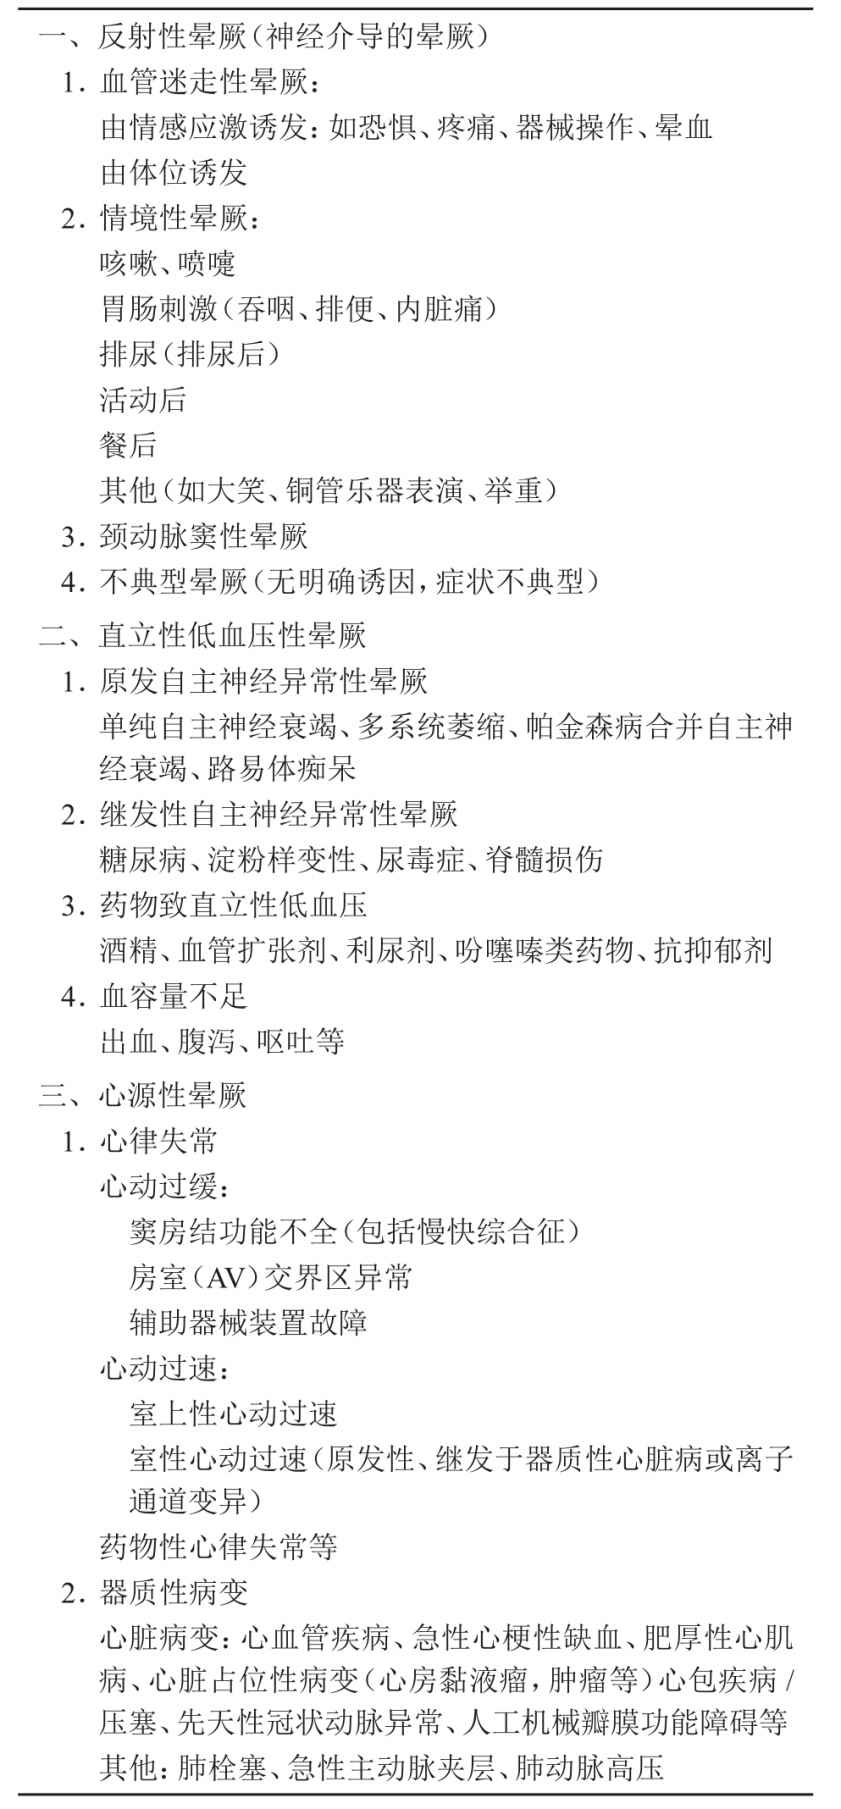
\includegraphics[width=3.30208in,height=7.11458in]{./images/Image00017.jpg}
\end{table}

\hypertarget{text00014.htmlux5cux23CHP1-4-1-1-1}{}
(1) 血管迷走性晕厥:

是最常见的晕厥类型,由情绪或直立位诱发,常伴自主神经激活的前驱症状(大汗、苍白或恶心)。

\hypertarget{text00014.htmlux5cux23CHP1-4-1-1-2}{}
(2) 情境性晕厥:

与一些特殊情境相关,如运动后晕厥等。

\hypertarget{text00014.htmlux5cux23CHP1-4-1-1-3}{}
(3) 颈动脉窦晕厥:

常由非机械性刺激因素诱发,可通过颈动脉窦按摩来确诊。

\hypertarget{text00014.htmlux5cux23CHP1-4-1-1-4}{}
(4) 不典型晕厥:

多数没有明确的诱发因素,诊断主要基于排除其他晕厥的病因(无器质性心脏病)。

\paragraph{直立性低血压和直立性不耐受综合征}

此类晕厥主要包括以下4种类型:

\hypertarget{text00014.htmlux5cux23CHP1-4-1-2-1}{}
(1) 典型的直立性低血压(OH):

站立3分钟内,收缩压下降≥20mmHg和(或)舒张压下降≥10mmHg,见于单纯性自主神经功能衰竭(ANF)、低血容量或其他形式的ANF。

\hypertarget{text00014.htmlux5cux23CHP1-4-1-2-2}{}
(2) 初始性直立性低血压:

站立即刻血压下降>
40mmHg,然后自发、快速地恢复正常,低血压及其症状持续时间较短(<
30秒)。

\hypertarget{text00014.htmlux5cux23CHP1-4-1-2-3}{}
(3) 延迟(进展性)OH:

其在老年人中并不少见,主要与年龄相关的代偿反射受损有关,以直立状态下收缩压进行性缓慢下降为特点,但不伴心动过缓。

\hypertarget{text00014.htmlux5cux23CHP1-4-1-2-4}{}
(4) 体位性直立性心动过速综合征:

部分患者(主要为年轻女性),表现为严重的直立性不能耐受,但没有晕厥,伴随心率明显加快(增加>
30次/分或达到120次/分以上)和血压不稳定,病理生理机制尚不明确。

\paragraph{心源性晕厥}

\hypertarget{text00014.htmlux5cux23CHP1-4-1-3-1}{}
(1) 心律失常性晕厥:

是心源性晕厥的最常见病因。心律失常诱发血流动力学不稳定,导致心输出量及脑血流量严重减少。心律失常类型包括:病窦综合征(窦房结功能受损,产生窦性停搏及窦房阻滞,以及慢-快综合征)和严重的获得性房室传导阻滞(莫氏Ⅱ型、高度及完全性房室传导阻滞),也可见于药物引起的缓慢性或快速性心律失常,如延长QT间期药物引起的尖端扭转性室速。

\hypertarget{text00014.htmlux5cux23CHP1-4-1-3-2}{}
(2) 器质性心脏病:

主要见于左室流出道梗阻性疾病。

\subsection{流行病学}

晕厥在普通人群中常见,首发年龄多为10~30岁,其中女性约47\%、男性约31\%在15岁左右发生晕厥。迷走性晕厥是导致晕厥的最主要原因,心源性晕厥是导致晕厥的第二位原因。医院中的老年患者心源性晕厥发病率较高。在小于40岁的患者中,OH所导致的晕厥较为少见。个别患者的病情较为复杂,在医疗转诊、救治的过程中,一些非晕厥的意识丧失患者常被误诊为晕厥。需注意的是,反射性晕厥是年轻人群中最为常见的导致TLOC的原因;而老年患者通常病情较为复杂,且相关病史也不及年轻人群可靠。

\subsection{诊断思路}

晕厥的诊断目的包括:①找出确切的原因以便进行有效的、针对病理机制的治疗;②识别患者的风险,这种风险常取决于潜在的疾病,而不是晕厥本身的机制。

\subsubsection{初步评估}

详细的病史询问在多数情况下有助于鉴别晕厥与非晕厥,但有时非常困难,应包含以下问题:

(1) 是否为完全性意识丧失(LOC)?

(2) LOC是否为一过性,伴快速起病及短暂持续?

(3) 患者晕厥是否为自发性、完全恢复且不留后遗症?

(4) 患者是否丧失肌张力?

若上述问题的答案均为肯定的,则晕厥可能性极大。若≥1个问题的答案为否定,则应首先排除其他类型的LOC。

对出现TLOC的患者进行初步评估,除了过去提出的详细询问病史、体格检查(包括测量不同体位血压)以及心电图检查外。提出在此基础上,可以适当增加其他的检查以保证诊断准确:①40岁以上患者建议首先进行颈动脉窦按摩。②对于有心脏病病史或怀疑此次晕厥与器质性心脏病或其他心血管疾病有关的患者,建议进行超声心动图检查。③对于怀疑因心律失常而导致晕厥的患者,应给予实时心电监测。④若晕厥与体位变化有关或怀疑反射性晕厥时,则应进行相关检查。如卧立位试验和(或)直立倾斜试验等。⑤仅在怀疑非晕厥原因造成的TLOC的情况下,进行神经科检查或血液检查。

当初步评估后尚无法明确晕厥原因时,要求立即对患者的主要心血管事件及心源性猝死(SCD)的风险进行评估。具体流程如图\ref{fig4-1}所示。

根据最新的SCD防治指南对晕厥进行了危险分层,见表\ref{tab4-2}。\footnote{LVEF:左室射血分数,SCD =心源性猝死,VT =室性心动过速,LBBB=左束支传导阻滞,RBBB =右束支传导阻滞,ARVC=致心律失常性右室心肌病,心衰=心力衰竭,心梗=心肌梗死}

经过初步评估有些晕厥即可明确诊断,其诊断的建议及级别、证据水平见表\ref{tab4-3}。

\begin{table}[htbp]
\centering
\caption{晕厥的危险分层}
\label{tab4-2}
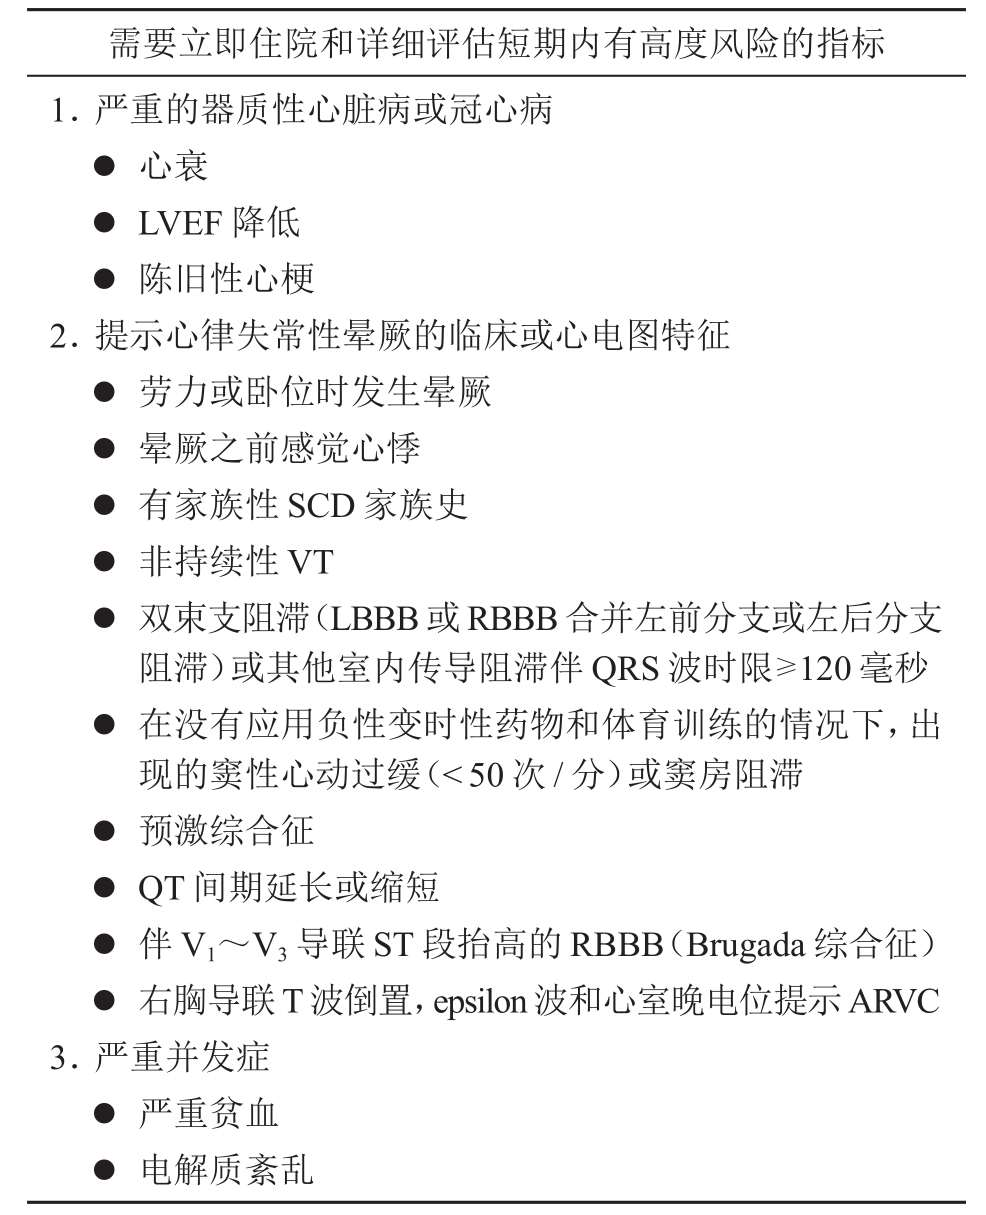
\includegraphics[width=3.28125in,height=4.04167in]{./images/Image00018.jpg}
\end{table}


\begin{figure}[!htbp]
 \centering
 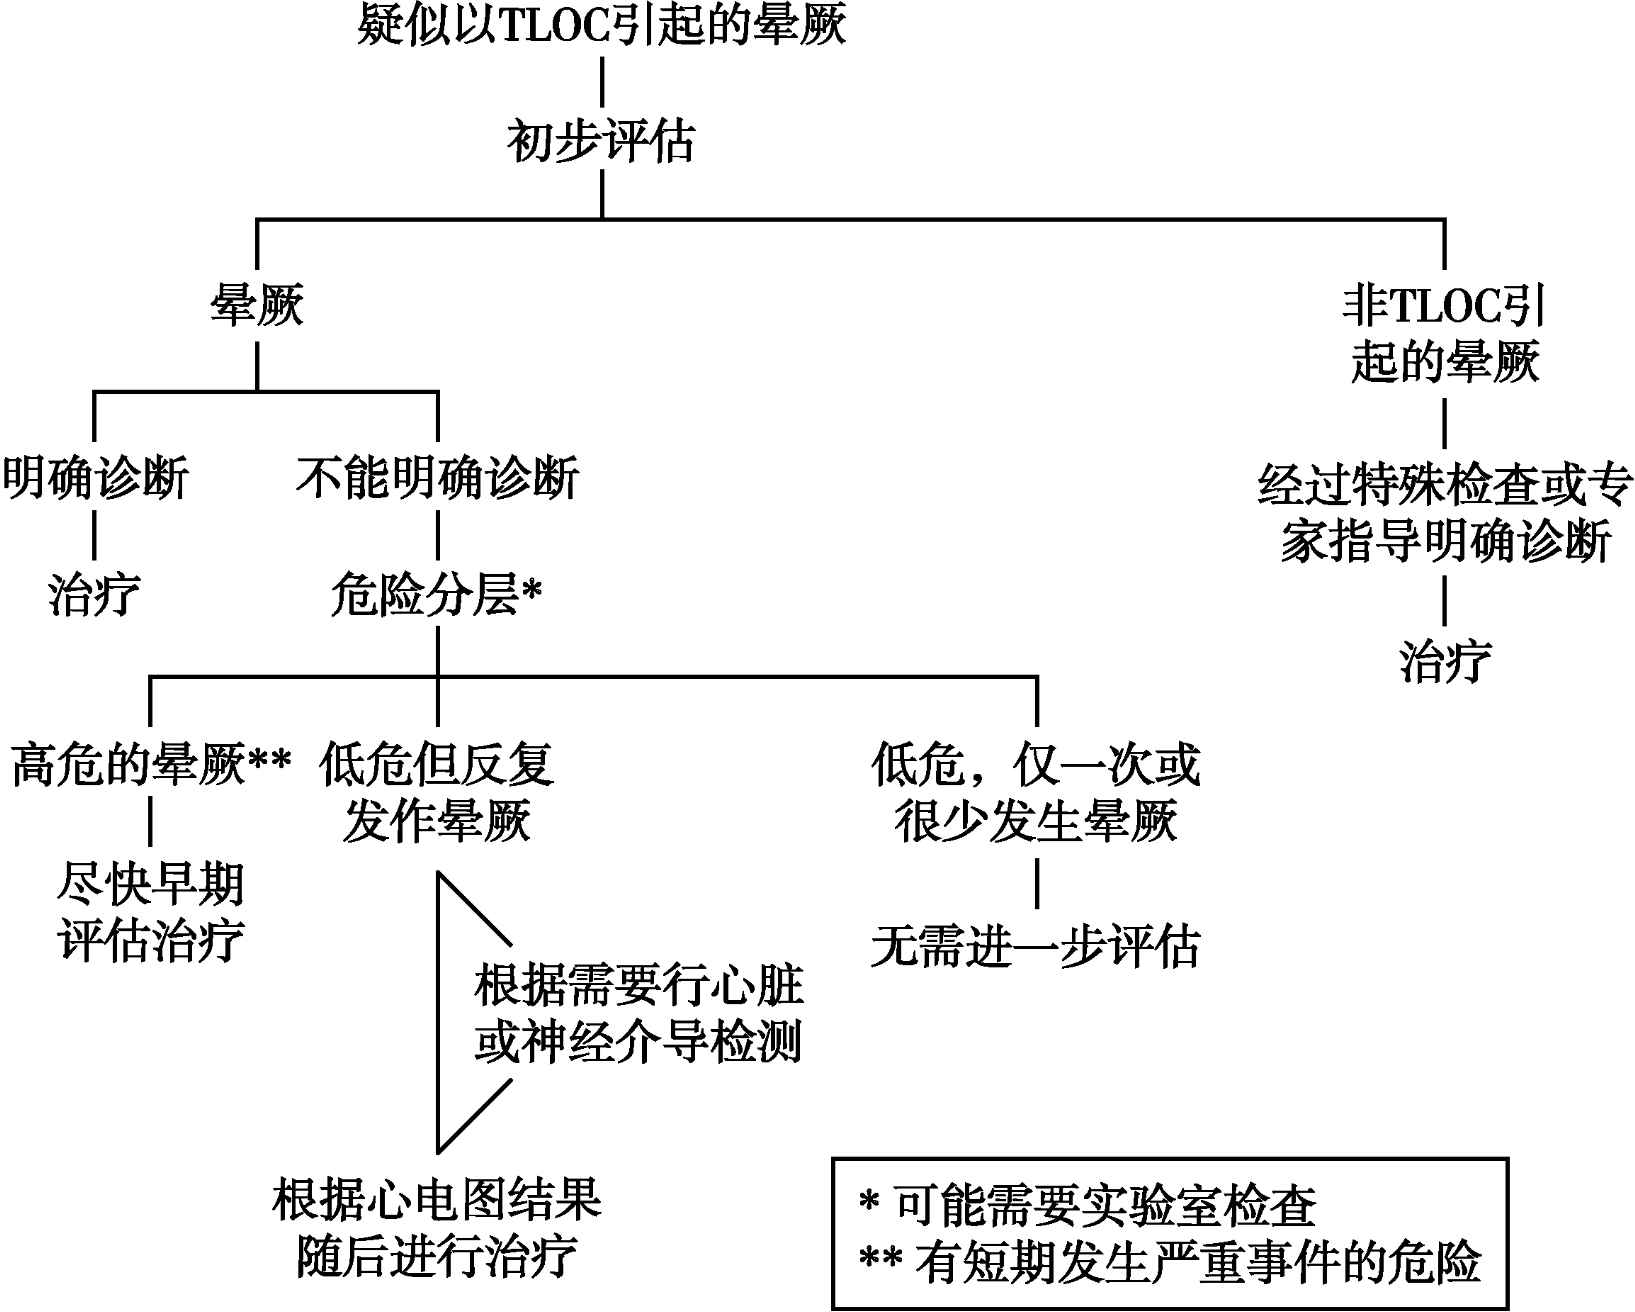
\includegraphics[width=3.84375in,height=3.08333in]{./images/Image00019.jpg}
 \captionsetup{justification=centering}
 \caption{疑似TLOC患者的诊断流程图}
 \label{fig4-1}
  \end{figure} 

\begin{table}[htbp]
\begin{center}
\caption{通过初步评估获得诊断的建议\textsuperscript{*}}
\label{tab4-3}
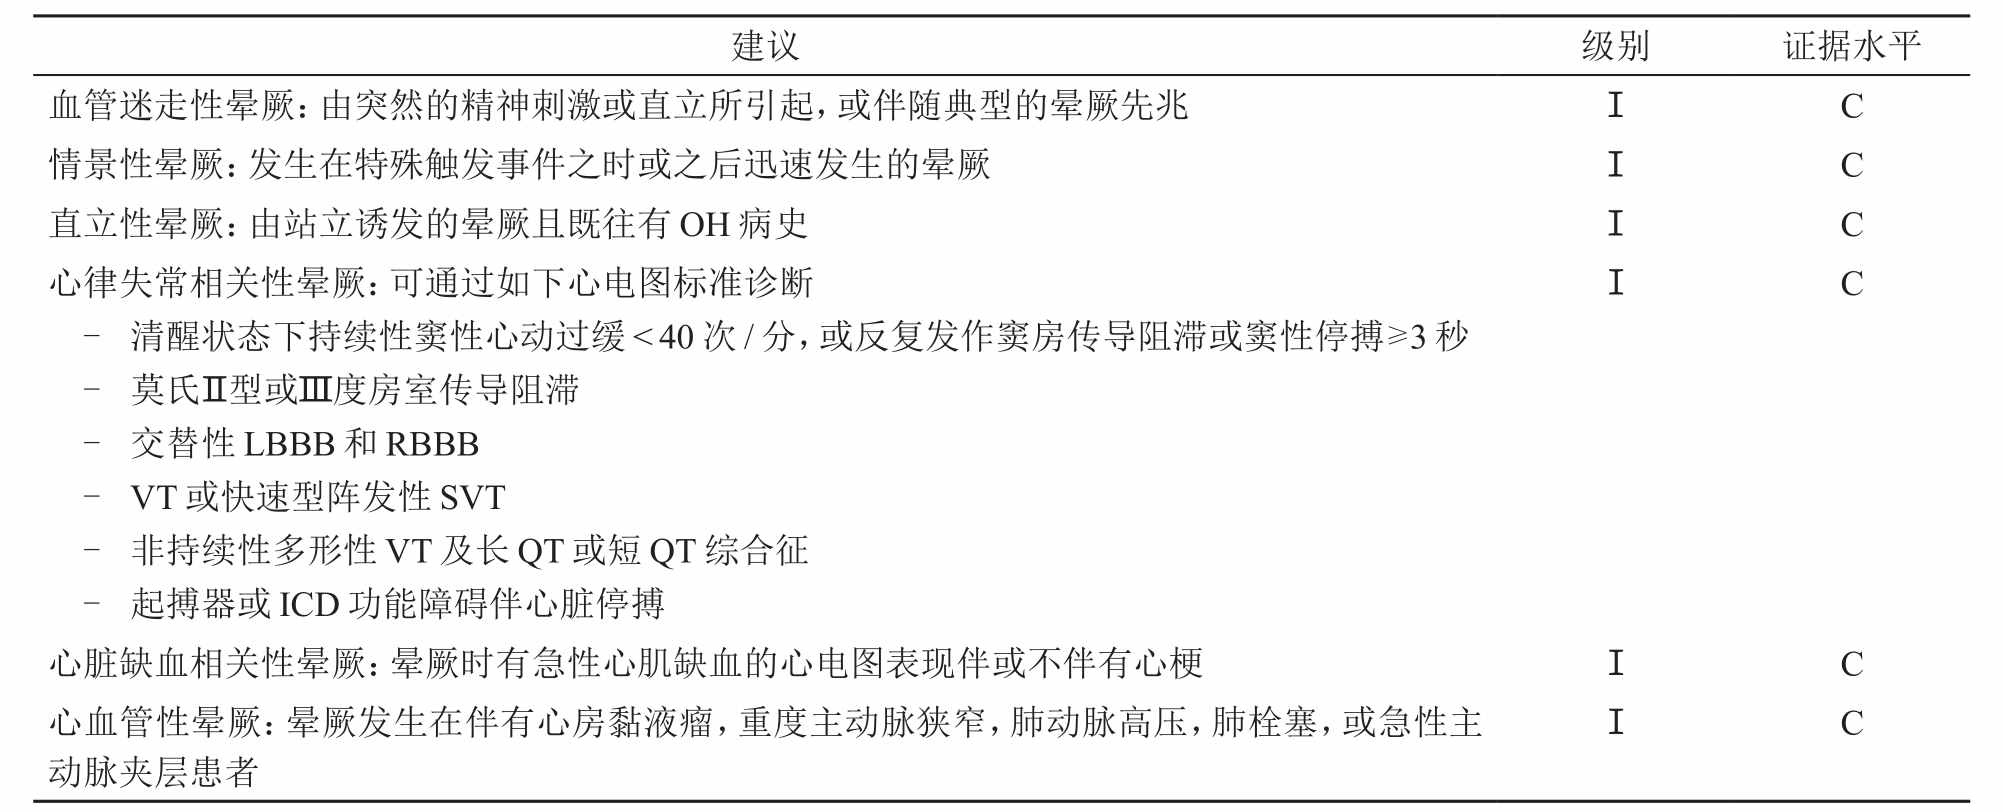
\includegraphics[width=6.66667in,height=2.69792in]{./images/Image00020.jpg}
\end{center}

{\small
*本文的建议均源自2009年ESC晕厥诊断和治疗指南。

建议的级别如下:

Ⅰ级:证据和(或)一致同意给予的诊断操作/处理有益,有用和有效。

Ⅱ级:抵触的证据和(或)关于处理的有用/有效存在分歧的观点。

Ⅱa级:证据/观点偏重于有用/有效。

Ⅱb级:证据/观点偏重于无用/无效。

Ⅲ级:证据或一致同意处理无用/无效,且在某些情况下可能有害。

证据水平如下:

A类证据:数据来自多中心随机临床试验或荟萃分析。

B类证据:数据来自单中心随机临床试验或大的非随机研究。

C类证据:专家的一致观点和(或)小的研究,回顾性研究,注册中心资料。}
\end{table}

\subsubsection{诊断试验}

初步评估后,倾向性诊断需要进一步检查证实,包括心脏评估检查如超声心动图,心脏负荷试验,心电监测包括Holter,必要时埋藏植入式心电事件记录仪(ILR)和电生理检查;神经介导方面的检查包括倾斜试验和颈动脉窦按摩。

\paragraph{颈动脉窦按摩}

压迫颈动脉分叉处能够产生反射性心率减慢和血压下降。某些晕厥患者,特别是>
40岁的患者,可以见到对颈动脉窦按摩的异常反应。室性停搏持续≥3秒,收缩压下降≥50mmHg为异常反应,称为颈动脉窦过敏。颈动脉窦按摩是揭示颈动脉窦过敏综合征晕厥的一种检查方法。2009年ESC晕厥诊断和治疗指南颈动脉窦按摩的适应证和诊断标准见表\ref{tab4-4}。

\begin{table}[htbp]
\centering
\caption{颈动脉窦按摩的适应证和诊断标准}
\label{tab4-4}
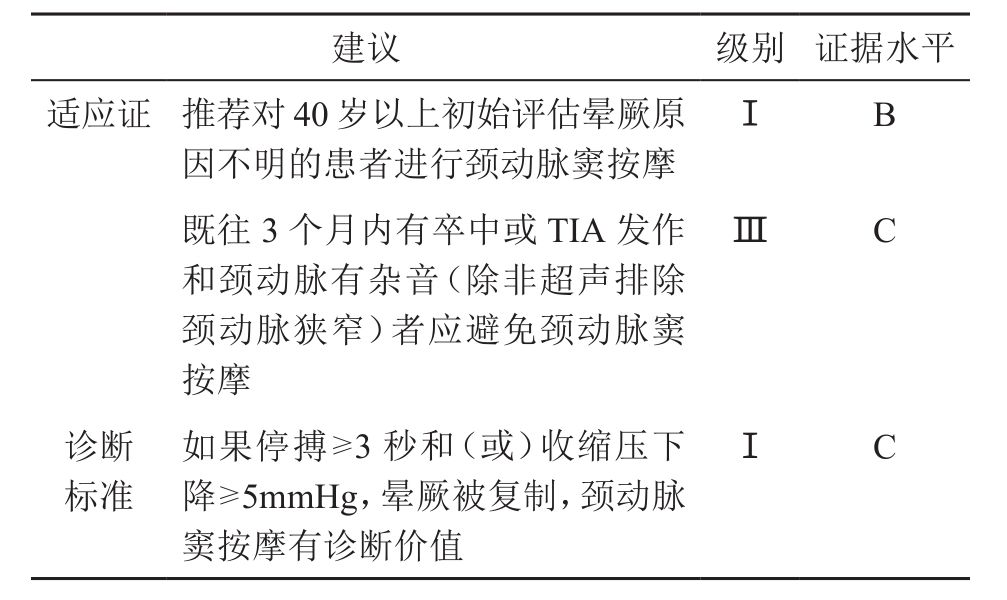
\includegraphics[width=3.34375in,height=1.98958in]{./images/Image00021.jpg}
\end{table}

\paragraph{倾斜试验}

倾斜试验有助于诊断神经介导性晕厥,但是,其敏感性、特异性、诊断标准和重复性存在很大问题,敏感性和特异性与检查方法有密切关系。敏感性26\%~80\%,特异性约90\%。2009年ESC晕厥诊断和治疗指南倾斜试验的适应证和诊断标准见表\ref{tab4-5}。

\paragraph{心电图}

(ECG)监测
ECG监测是诊断间歇性缓慢和快速心律失常的方法,但是ECG监测技术目前仍有严重的局限性。晕厥患者ECG监测的作用不是孤立的。医生可以根据病史、体格检查和其他客观检查如倾斜试验决定治疗方案。有些情况下,临床上强烈提示为反射性晕厥时,无需动态心电图(Holter)监测。如果症状发作不频繁Holter监测对诊断意义也不大,这种情况下应考虑植入式循环记录仪。将来的技术可能会记录ECG以外的多项指标,将把重点放在与自发性晕厥相关的心律方面,而不是被触发的晕厥。了解自发性晕厥发作过程是评估晕厥的最好标准。因此,植入式监测仪对晕厥越来越重要。记录到晕厥时有缓慢心律失常即可考虑诊断,但是,有时需要进一步检查明确是心脏本身原因所致还是神经反射机制造成,而反射性心动过缓可能是阵发性心动过缓最常见的原因。

由于晕厥发作时ILR记录到的心律失常的变异和干扰很大,2009年ESC晕厥诊断和治疗指南采用国际不明原因晕厥研究调查组织(ISSUE)的方法,将心电图记录进行了分类,根据主要心律失常和可能的晕厥机制将心电图划分为4型。

1型:心脏停搏,RR间期≥3秒。1型又分为A、B、C
3个亚型。1A型:窦性停搏,表现为进行性窦性心动过缓或初为窦性心动过速逐渐进展为窦性心动过缓直至发生窦性停搏,其可能的机制为反射性。1B型:窦性心动过缓合并房室传导阻滞,表现为进行性窦性心动过缓随后出现房室传导阻滞(和心室停搏)的同时伴有窦率下降;或突发房室传导阻滞(和心室停搏)伴窦率下降,其可能机制为反射性。1C型:房室传导阻滞,突发房室传导阻滞(和心室停搏)伴窦律逐渐增加,其可能机制为自身病变。

2型:心动过缓,心率下降> 30\%或心率<
40次/分持续超过10秒,其可能机制为反射性。

3型:无或很小的心率变异性,心率变异度< 30\%且心率>
40次/分,其机制不肯定。

4型:心动过速,心率增加> 30\%,心率> 120次/分。此型又分为A、B、C、D
4型。4A型:进行性窦性心动过速,机制不肯定。4B型:心房颤动(简称房颤)。4C型:SVT(不包括窦性)。4D型:VT。

\begin{table}[htbp]
\centering
\caption{倾斜试验的适应证和诊断标准}
\label{tab4-5}
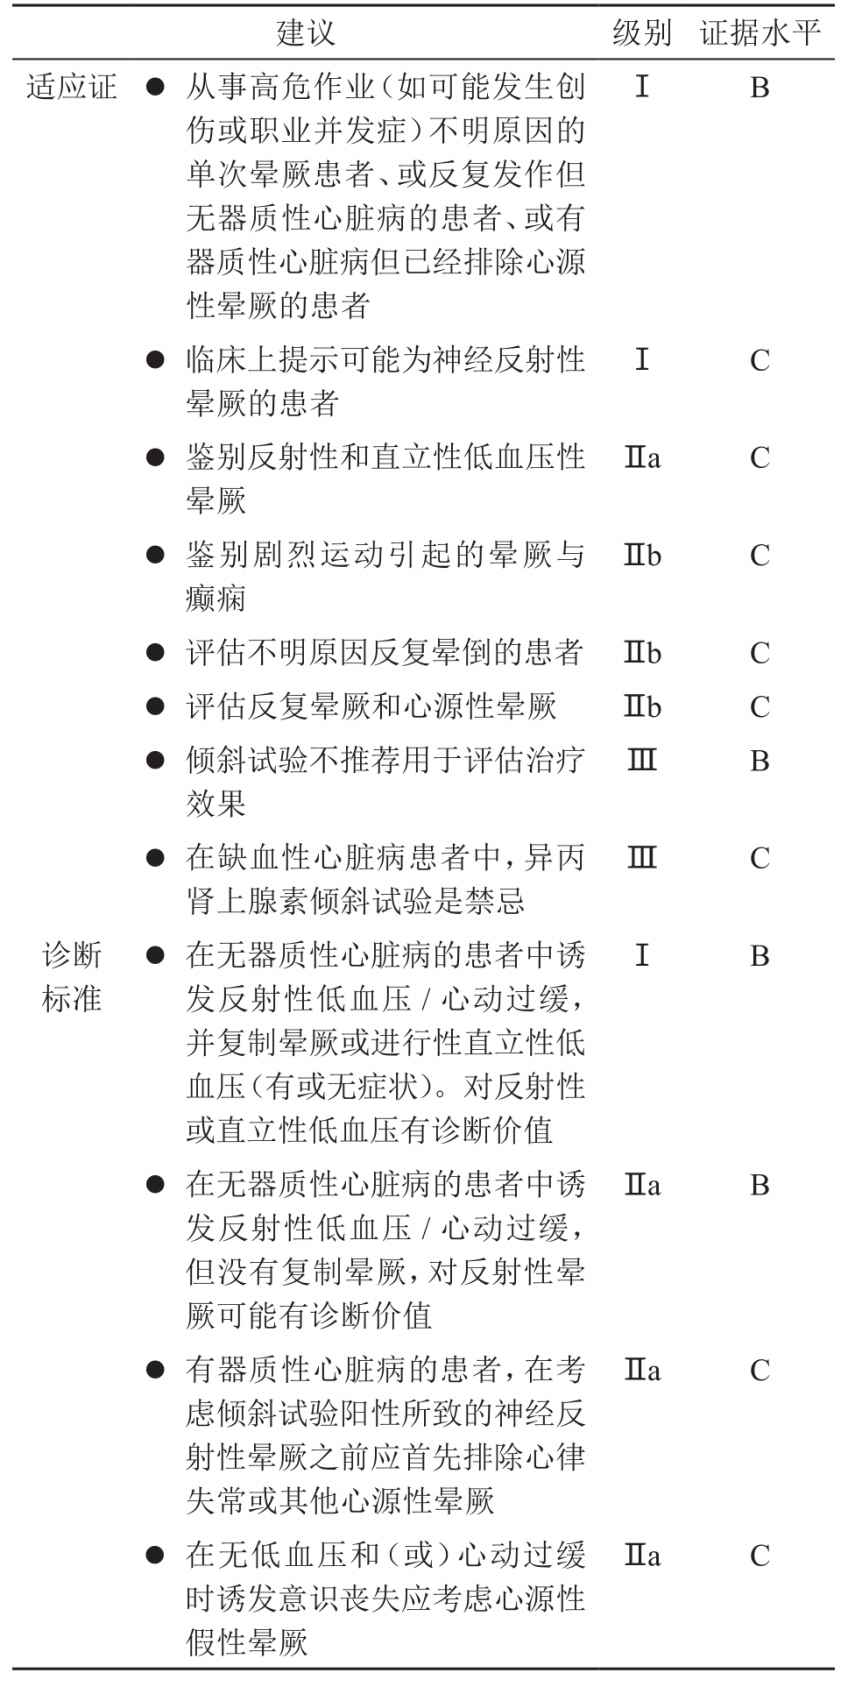
\includegraphics[width=3.21875in,height=6.40625in]{./images/Image00022.jpg}
\end{table}

2009年 ESC晕厥诊断和治疗指南心电图监测的建议见表\ref{tab4-6}。

\paragraph{电生理检查}

电生理检查通过心内膜和心外膜(冠状窦电极)刺激并记录揭示引起晕厥的原发性心律失常的心电异常改变。然而,仅有少数研究应用Holter和植入式记录仪证实了电生理检查的结果。电生理检查揭示的真实诊断仅仅涵盖了一部分患者。下列诊断标准广泛用于确定窦房结功能障碍:窦房结恢复时间(SNRT)>
1.6秒或2秒或校正的窦房结恢复时间(CSNRT)> 525毫秒。另一项研究认为SNRT
>
3秒诊断窦房结功能障碍性晕厥的可能性更大。2009年ESC晕厥诊断和治疗指南电生理检查的适应证见表\ref{tab4-7}。\footnote{ARVC:致心律失常型右室心肌病;HCM:肥厚型心肌病}

\begin{table}[htbp]
\centering
\caption{心电图监测的建议}
\label{tab4-6}
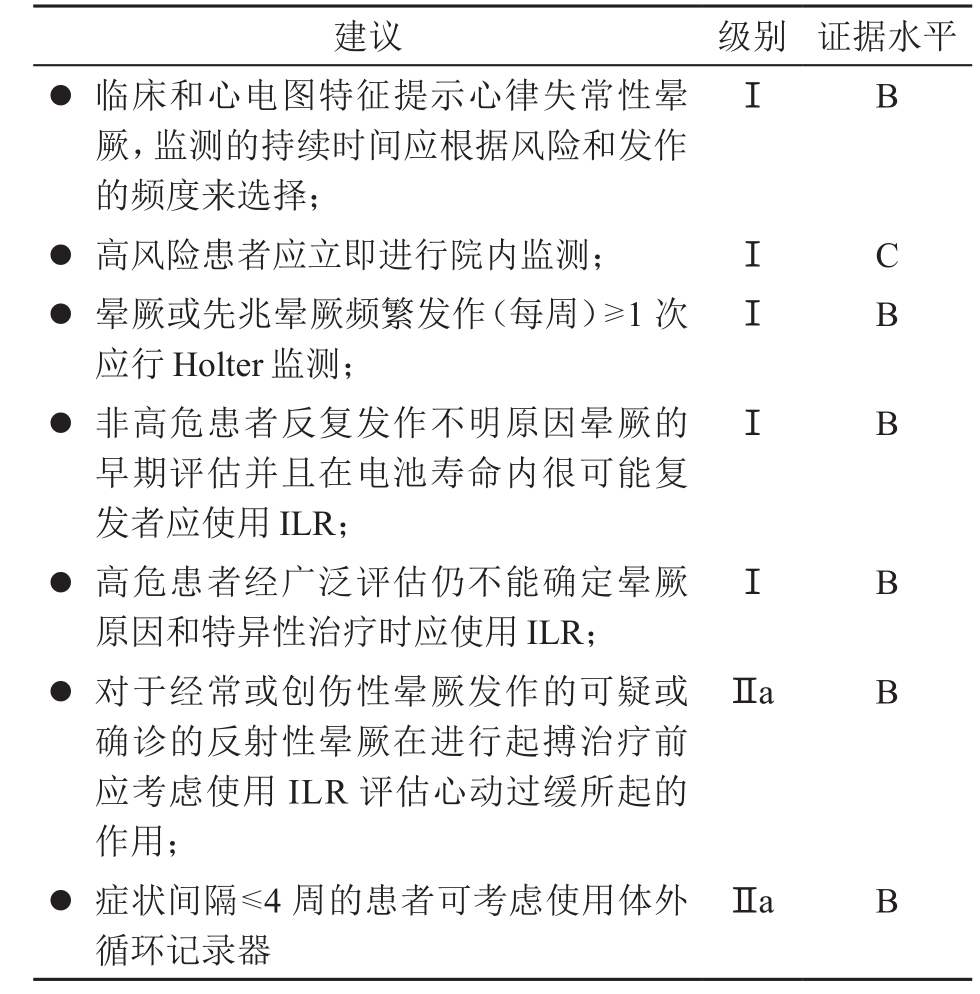
\includegraphics[width=3.25in,height=3.30208in]{./images/Image00023.jpg}
\end{table}

\begin{table}[htbp]
\centering
\caption{电生理检查的适应证}
\label{tab4-7}
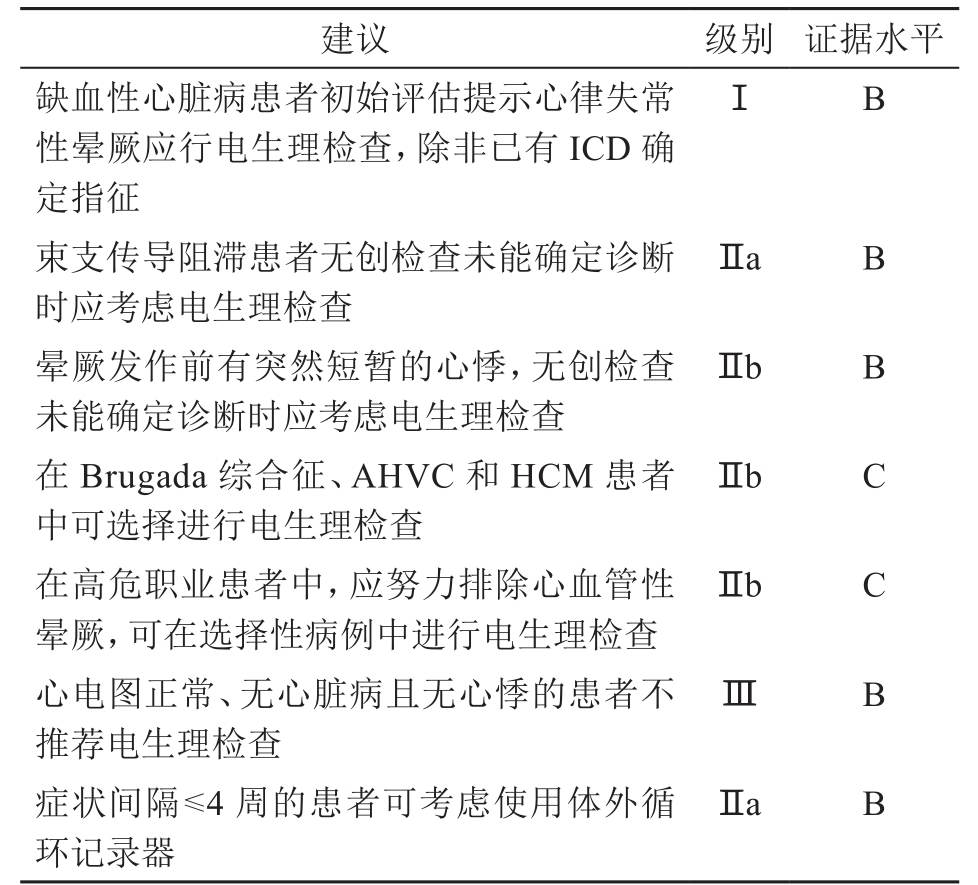
\includegraphics[width=3.25in,height=2.9375in]{./images/Image00024.jpg}
\end{table}



\paragraph{超声心动图(UCG)}

当病史、体格检查和心电图检查不能发现晕厥的原因时,超声心动图检查是发现包括瓣膜病在内的器质性心脏病的有效方法。通过该检查还能发现肺动脉高压和右心室扩大等提示肺栓塞的表现。体格检查正常的晕厥或先兆晕厥患者超声心动图检查最常见的发现是二尖瓣脱垂(4.6\%~18.5\%)。其他心脏异常包括瓣膜病(最常见的是主动脉瓣狭窄)、心肌病、节段性室壁运动异常提示的心肌梗死、冠状动脉畸形、浸润性心脏病如淀粉样变性、心脏肿瘤、动脉瘤、左房血栓等。超声心动图检查为判断晕厥的类型、严重程度及危险分层提供重要的信息。如果发现中重度器质性心脏病应考虑心源性晕厥。另一方面,如果超声心动图仪发现轻微心脏结构病变,则心源性晕厥的可能性较小,应进行非心源性晕厥方面的检查。2009年ESC晕厥诊断和治疗指南UCG适应证和诊断标准见表\ref{tab4-8}。

\begin{table}[htbp]
\centering
\caption{UCG适应证和诊断标准}
\label{tab4-8}
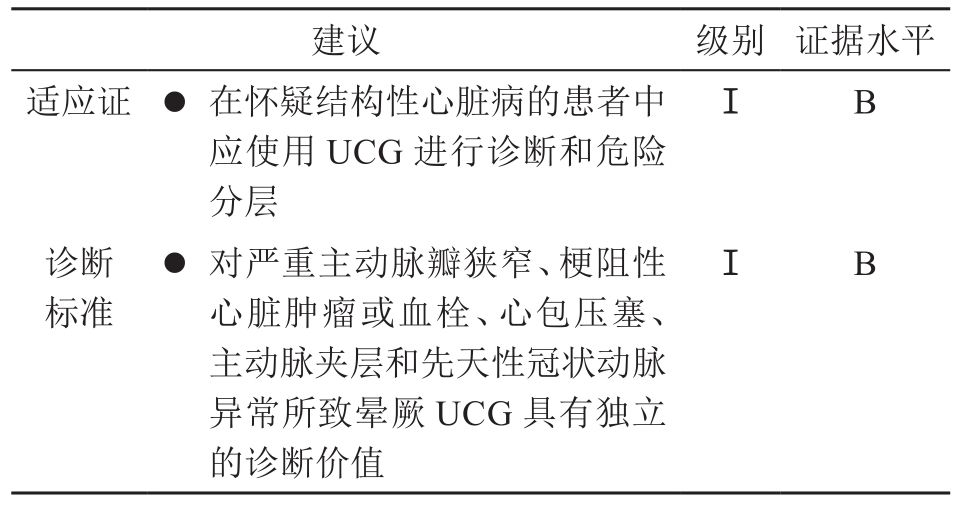
\includegraphics[width=3.20833in,height=1.6875in]{./images/Image00025.jpg}
\end{table}

\paragraph{运动试验}

运动中或运动后即刻发生晕厥的患者应进行运动试验。进行运动试验应该是症状限制性的,即由于运动中和运动后即刻易发生晕厥,运动中和恢复阶段均应监测心电和血压,应做好防范。运动中发生晕厥可能是心脏原因造成的,有些病例报告运动中也可能发生过度反射性血管扩张引起晕厥,反射性晕厥的元凶是低血压而无心动过缓。相反,运动后晕厥几乎都是自主神经功能异常或神经介导机制参与的,其特点是与心动过缓或心脏停搏有关的低血压;一般发生于无心脏病的患者。运动试验用于诊断神经反射性晕厥,其特点是劳力后晕厥。血管迷走神经性晕厥的患者,运动中内脏容量性血管和前臂阻力血管反射性收缩功能障碍。运动试验对一般晕厥患者意义不大,仅有1\%发现异常。尽管如此,对运动性晕厥具有重要诊断价值。2009年ESC晕厥诊断和治疗指南运动试验的适应证和诊断标准见表\ref{tab4-9}。

\begin{table}[htbp]
\centering
\caption{运动试验的适应证和诊断标准}
\label{tab4-9}
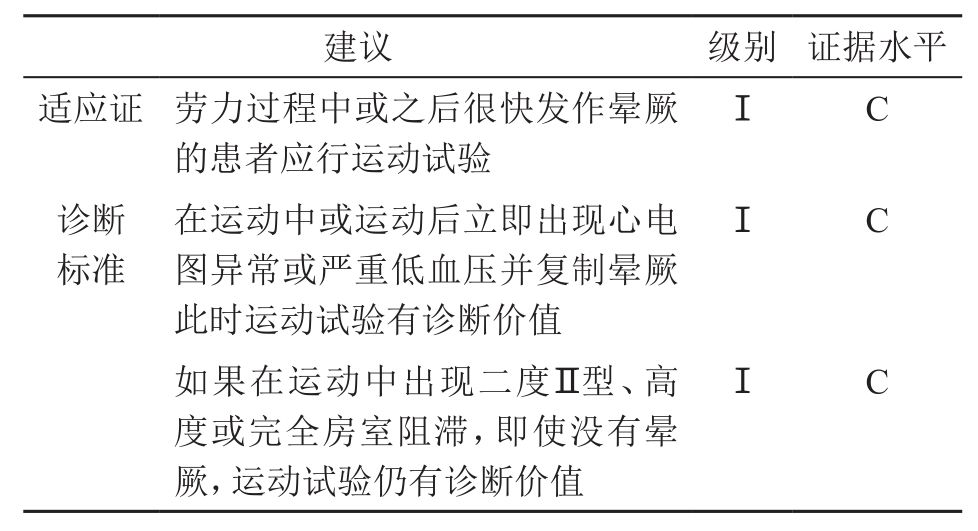
\includegraphics[width=3.25in,height=1.76042in]{./images/Image00026.jpg}
\end{table}

\paragraph{心导管检查}

心导管检查包括评估心腔形态的心室造影、了解冠脉解剖的冠状动脉造影和了解血流、血管内压力和心腔内压力的血流动力学检查。由于是有创检查,一般不作为筛查心源性晕厥的检查。这些检查能够揭示冠状动脉狭窄引起缺血性晕厥:室壁运动异常和心肌收缩力减弱;缺血引起的心律失常、心脏停搏或完全性房室阻滞和缺血诱发的血管迷走神经性反应。也可以揭示冠状动脉痉挛引起的晕厥,这种患者冠状动脉造影中应做麦角新碱试验。

\paragraph{神经系统检查}

神经系统疾病引起的晕厥有三种情况。①自主神经功能障碍:晕厥可以是自主神经系统疾病和功能不全的结果;②有些脑血管疾病也可以引起晕厥(大多是“窃血”综合征);③有些疾病应列为鉴别诊断的内容,因为这些疾病可以引起短暂意识丧失(但不是晕厥,如癫痫)或其发作类似于意识丧失。2009年ESC晕厥诊断和治疗指南神经系统检查适应证见表\ref{tab4-10}。

\begin{table}[htbp]
\centering
\caption{神经系统检查适应证}
\label{tab4-10}
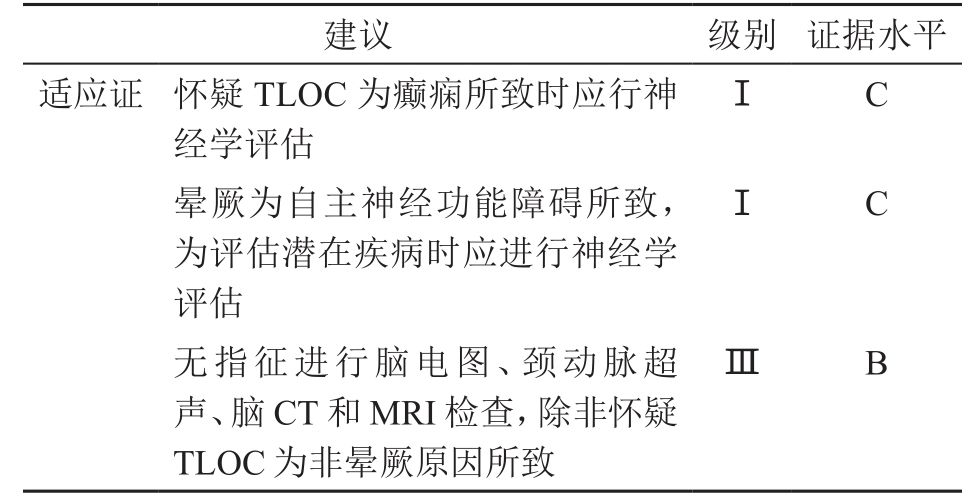
\includegraphics[width=3.25in,height=1.66667in]{./images/Image00027.jpg}
\end{table}

\subsubsection{诊断注意事项}

对所有一过性意识丧失患者必须进行全面仔细的评估,包括病史和检查。要顺序确认:是否晕厥,晕厥的原因,死亡和其他风险。尽管从死亡率角度来说,晕厥常常是良性的,但仅仅确定患者是低死亡风险患者是不够的,因为晕厥常常会复发,增加外伤风险,并且影响生活质量和正常工作。晕厥的诊断和治疗是富于挑战性的。首先,晕厥仅仅是一过性意识丧失众多原因中的一种;其次,患者症状短暂,就诊时一般都已完全恢复,并且有价值的查体发现很少;第三,自发的临床事件很少被医学专业人员目击,临床事件的病史经常是来自“二手”甚至“三手”的资讯。急诊科医生应仔细考虑所发现的异常是否和临床情况相匹配,强调长程监测的重要性。为了使患者得到准确的预后评估和治疗选择,强调应尽可能确定患者的病因。

\subsection{治疗}

\subsubsection{晕厥治疗的一般原则}

晕厥治疗的一般原则是:延长生命、预防复发、防治躯体损伤。

采取基础预防性治疗还是加强治疗取决于下列临床情况:①晕厥的病因。②晕厥复发的可能性大小。③晕厥的死亡危险性大小,主要取决于心脏病和血管病的性质和严重程度。④复发次数或晕厥导致躯体或精神伤害的危险性大小。⑤发生晕厥可能对个人职业或业余爱好造成的影响(如个人经济和生活方式问题)。⑥对公共健康的危险性如汽车司机、飞行员等。⑦对治疗有效性、安全性和不良反应的评估(特别要考虑患者的伴随疾病)。根据晕厥不同病因和机制以及危险分层,采取不同的治疗策略。晕厥的治疗流程见图\ref{fig4-2}。

\paragraph{反射性晕厥的治疗}

反射性晕厥包括血管迷走神经性晕厥、颈动脉窦综合征(CCS)和情景性晕厥,其治疗目标首先是预防症状复发和晕厥相关的损伤,改善生活质量。自2004年指南发表后,治疗方面最大的进展是在生活方式方面上,反射性晕厥非药物治疗的基石是教育,让患者相信这是一种良性情况。一般来讲,最初的治疗涉及让患者了解这一疾病及如何避免诱因(如闷热而拥挤的环境,血容量不足)等相关方面的教育。早期识别前驱症状,采取某些动作以终止发作{[}如仰卧位,身体反压调整(PCMs){]}。避免引起血压降低的药物(包括α受体阻滞剂、利尿剂和酒精)。对于不可预测的频繁发作的晕厥需给予其他治疗。特别是:①非常频繁发作影响到生活质量;②反复晕厥没有或仅有非常短时的晕厥先兆,但患者暴露于有外伤危险的情况下;③晕厥发生在高危作业时(如驾驶、操作机器、飞行、竞技性体育运动等)。

具体治疗方法如下:①身体反压调整(PCMs):非药物的物理治疗,为反射性晕厥的一线治疗。PCMs即双腿肌肉等长收缩PCMs(双腿交叉),或双上肢肌肉等长收缩PCMs(双手紧握和上肢紧绷),多中心前瞻性研究显示,使用这种方法,在反射性晕厥发作时能够显著升高血压,多数情况下可使患者避免或延迟意识丧失。②倾斜训练:可能会减少晕厥复发,但是患者依从性较差,治疗受到影响。③药物治疗:许多试图用于治疗反射性晕厥的药物结果都令人失望。这些药物包括β受体阻滞剂、丙吡胺、东莨菪碱、茶碱、麻黄碱、依替福林、米多君、可乐定和5-羟色胺重吸收抑制剂。由于在反射性晕厥时外周血管常常不能得到适当的收缩,α受体激动血管收缩剂(依替福林和米多君)曾被使用,但是,治疗效果不一致。专家组认为,反射性晕厥患者长期单独使用α受体激动剂药物治疗可能有一些作用,对于偶发患者不建议长期治疗。在长时间站立或从事常常诱发晕厥的活动前1小时服用单剂量的药物避免晕厥发生,对有些患者可能有用。④心脏起搏:起搏治疗反射性晕厥的随机对照试验得出了相反的结果。专家组认为在迷走神经性晕厥中血管减压部分通常起主要作用,所以得出起搏欠佳的结果并不奇怪。而颈动脉窦晕厥心脏起搏治疗可能有效,双腔起搏一般优于单腔心室起搏。反射性晕厥治疗的建议见表\ref{tab4-11}。\footnote{CSS =颈动脉窦综合征;VVS =血管迷走晕厥}

\begin{figure}[!htbp]
 \centering
 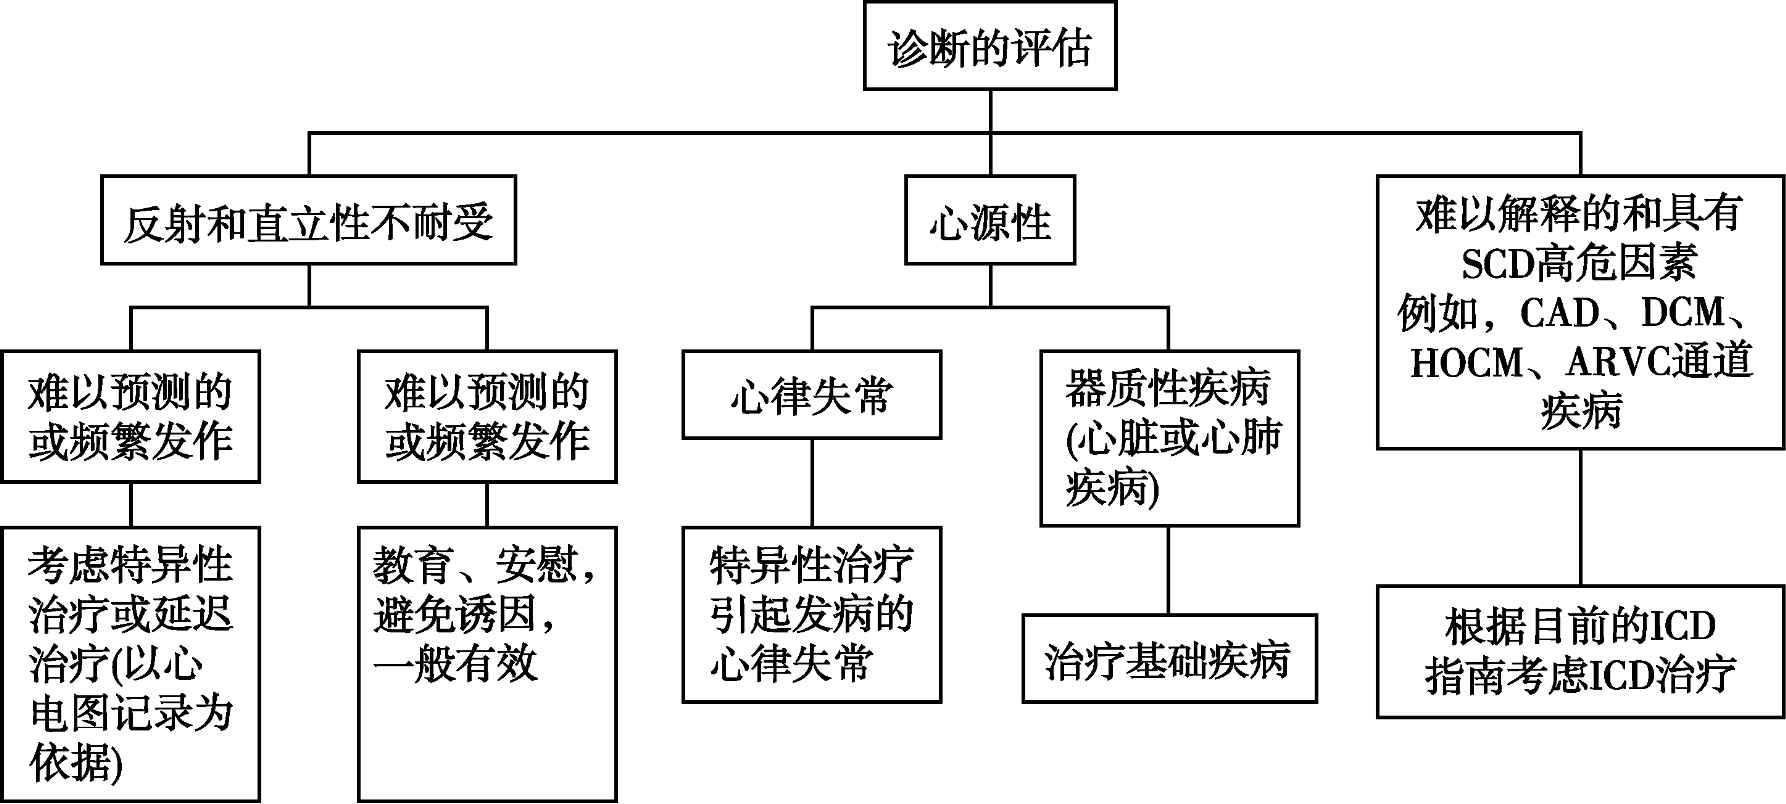
\includegraphics[width=4.82292in,height=2.16667in]{./images/Image00028.jpg}
 \captionsetup{justification=centering}
 \caption{晕厥的治疗流程}
 \label{fig4-2}
  \end{figure} 

\begin{table}[htbp]
\centering
\caption{反射性晕厥的治疗建议}
\label{tab4-11}
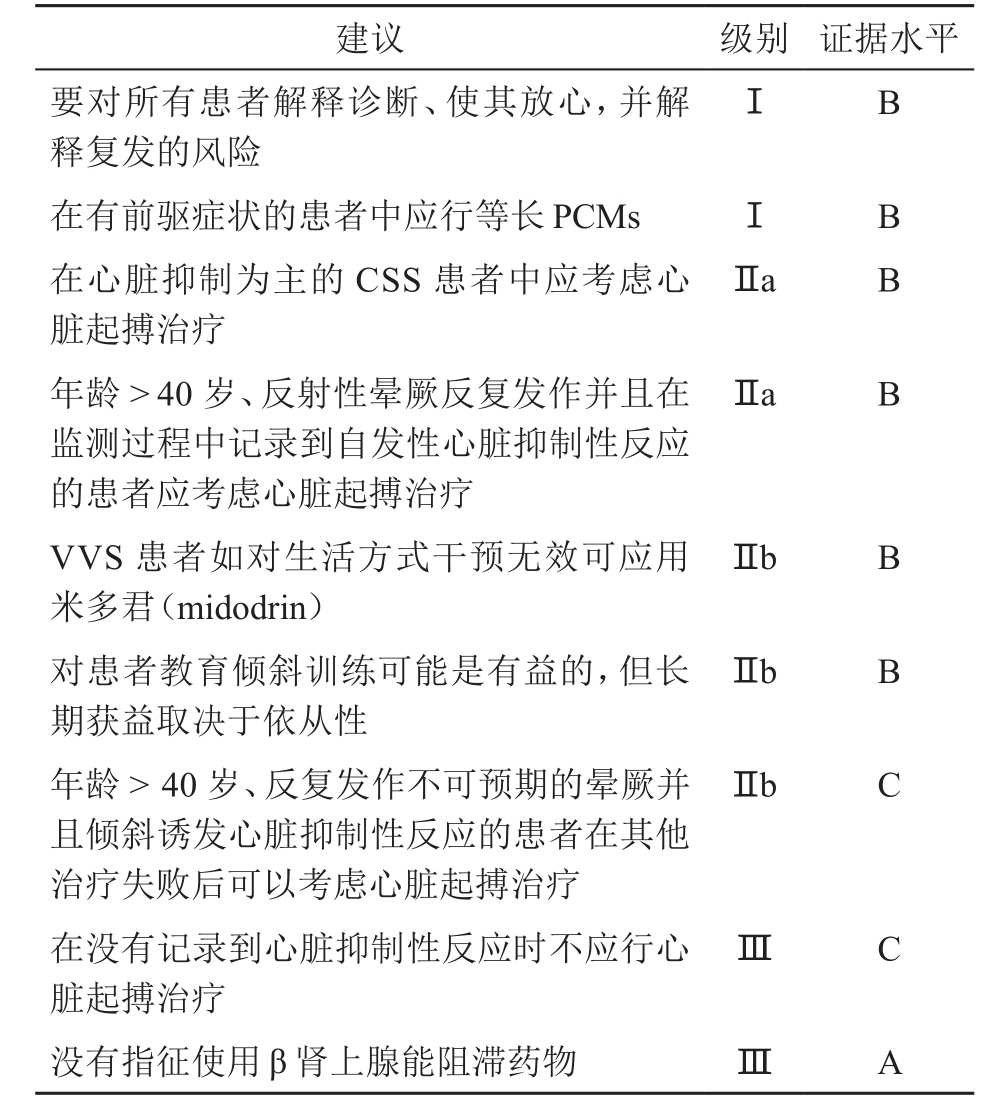
\includegraphics[width=3.28125in,height=3.66667in]{./images/Image00029.jpg}
\end{table}


\paragraph{直立性低血压的治疗}

治疗目标是预防症状复发以及晕厥造成的伤害,改善生活质量。药物诱发的自主神经功能失调可能是直立性低血压性晕厥最常见的原因,主要治疗方法是停药,仅有少数患者由于病情不能停药。引起直立性低血压最常见的药物是利尿剂和血管扩张剂,酒精也是常见的原因,其除诱发自主神经性晕厥外还可引起躯体神经系统疾病。包括对中枢神经系统的直接作用和血容量不足。主要治疗是戒酒。对于原发性和继发性自主神经功能失调的患者,了解血压调节的生理和病生理机制十分重要,治疗的主要目标是改善由于脑灌注不足导致的症状(如晕厥、先兆晕厥、意识模糊等)。尽管通过上述治疗使收缩压升高幅度不大(10~15mmHg),但可以明显改善直立性低血压的症状;使平均动脉压升高恰到好处,重新达到自主神经的调节范围内,进而可以明显改善神经调节功能。应对所有患者进行健康教育,使他们了解影响血压的因素,避免突然站起(尤其是醒后)、长时间站立、白天长时间卧位休息、用力排尿排便、过度通气、高温环境(包括热澡水、淋浴、桑拿浴)、极度用力、暴食(特别是精制的碳水化合物)、具有扩血管作用的酒精和药物。动态监测血压有助于了解白天不同环境中的血压变化,了解高血压患者药物对卧位/夜间血压的影响。扩张细胞外容量是重要的治疗目标。对无高血压的患者,应指导摄入足够的盐和水。每天达到2~3L液体和10g氯化钠。快速摄入冷开水对运动中或餐后低血压者有明显疗效;高枕位睡眠(头部抬高10°)可防止夜间多尿,维持适量的体液量及改善夜间高血压。老年患者可佩戴腹带或加压弹力袜以减轻下肢血液蓄积;有先兆晕厥时可采取交叉腿和蹲位姿势等预防措施。α受体激动剂(米多君)是慢性自主神经异常者的首选药物。氟氢可的松(0.1~0.3mg/d)可促进钠水潴留及扩张血容量,改善晕厥症状。其他治疗如去氨加压素用于伴夜尿增多者;奥曲肽用于餐后低血压,促红细胞生成素用于贫血者等。直立性低血压治疗建议见表\ref{tab4-12}。

\begin{table}[htbp]
\centering
\caption{直立性低血压的治疗建议}
\label{tab4-12}
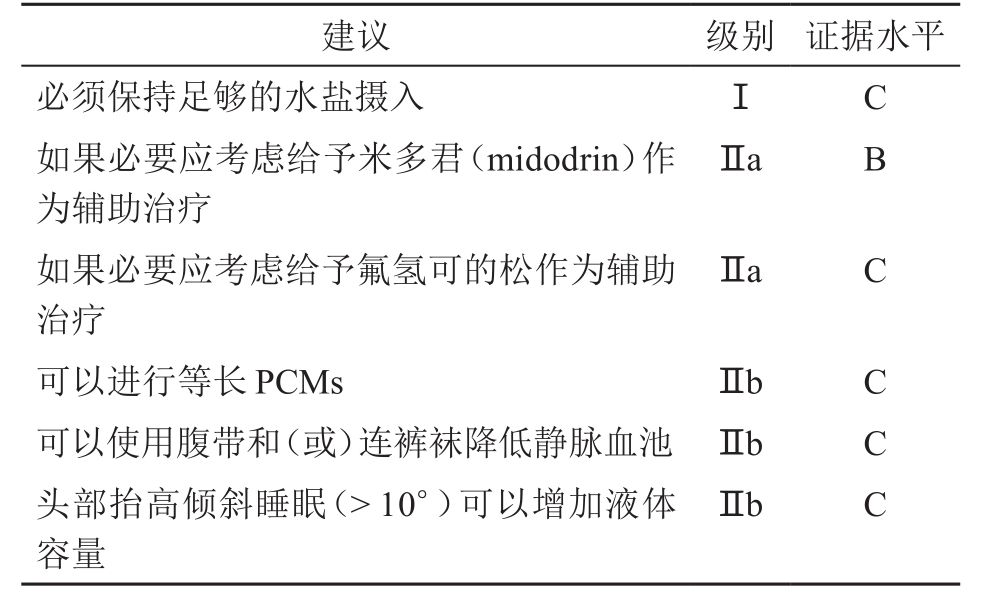
\includegraphics[width=3.27083in,height=2in]{./images/Image00030.jpg}
\end{table}

\paragraph{心律失常性晕厥的治疗}

治疗目标预防症状复发,改善生活质量,减低死亡危险。原发性心律失常与心脏本身疾病或解剖异常有关,是最常见晕厥原因之一。包括原发性窦房结功能异常(缓慢、快速心律失常)、传导系统病变、室上性心动过速和室性心动过速。这种晕厥的基础是多方面的,包括心律失常的频率、左心室的功能状态和血管的代偿作用(包括神经反射作用)。

\hypertarget{text00014.htmlux5cux23CHP1-4-4-1-3-1}{}
(1) 窦房结功能不全:

窦房结功能不全伴缓慢心律失常、或SNRT异常引起的晕厥,起搏治疗效果显著。永久起搏可明显缓解症状,但对生存率无影响。预防晕厥复发的另一主要措施是停用加重或诱发心动过缓的药物,如无合适的替代药物应行心脏起搏。

\hypertarget{text00014.htmlux5cux23CHP1-4-4-1-3-2}{}
(2) 房室传导系统疾病:

AV阻滞引起的晕厥需起搏治疗,永久右室心尖部起搏的危害已获证实,但其替代起搏位点仍有争议。AV阻滞伴LVEF下降、心力衰竭(心衰)及QRS间期延长所致者可考虑双腔起搏。

\hypertarget{text00014.htmlux5cux23CHP1-4-4-1-3-3}{}
(3) 阵发性室上性和室性心动过速:

阵发性室上性和室速或典型心房扑动引起的晕厥,应首选导管消融术。尖端扭转型室速所致的晕厥主因是应用引起QT间期延长的药物所致,应立即停药。心功能正常或轻度受损者,如出现室速伴晕厥,可考虑导管消融或药物治疗。心功能不全、室速或心室颤动伴晕厥且病因无法祛除者应植入埋藏式心脏复律除颤器(ICD)。ICD虽不能有效预防晕厥复发,但可降低猝死风险。心律失常性晕厥的治疗见表\ref{tab4-13}。

\paragraph{SCD高危患者不明原因晕厥的治疗}

其治疗目标不仅仅是防止晕厥再发,而且要治疗基础疾病和减少SCD的风险。严重主动脉狭窄或心房黏液瘤所致的晕厥可考虑手术治疗;继发于急性心血管事件如肺栓塞、心肌梗死或心包压塞者主要针对病因治疗;大多数心肌缺血所致者可采用药物和(或)血管重建;由原发性肺动脉高压或限制性心肌病引起者,一般不易纠正原发病。急、慢性冠状动脉疾病或LVEF下降均可增加死亡风险,故需评估缺血的严重程度,且如果有适应证应考虑血运重建。但血运重建并不能改善恶性心律失常引起的不良后果,因此该类患者应行电生理检查以评估有无心律失常。心衰且符合最新指南制定的ICD适应证者,无论晕厥发生机制是否明确,均应植入ICD。有研究显示,植入ICD的晕厥患者生存率明显增加;不明原因晕厥的缺血性或非缺血性心肌病伴心衰或LVEF严重下降者应植入ICD(Ⅰ类,A级);LVEF正常和电生理检查阴性者不建议植入ICD。其他类型心脏病:①肥厚性心肌病伴不明原因晕厥尤其是发作间期短(<
6个月)、相对危险度>
5的患者,其猝死风险较高;植入ICD效果明显。②约1/3致心律失常性右室心肌病(ARVC)者会发生晕厥。年轻、严重右室发育不全、左室功能障碍、多形性室速、心室晚电位、epsilon波及有猝死家族史者,如无其他病因应考虑植入ICD。③遗传性离子通道异常性心脏病常以晕厥为先兆表现,但该类患者是否应植入ICD仍有争议。SCD高危晕厥患者ICD适应证见表\ref{tab4-14}。

\begin{table}[htbp]
\centering
\caption{心律失常性晕厥的治疗建议}
\label{tab4-13}
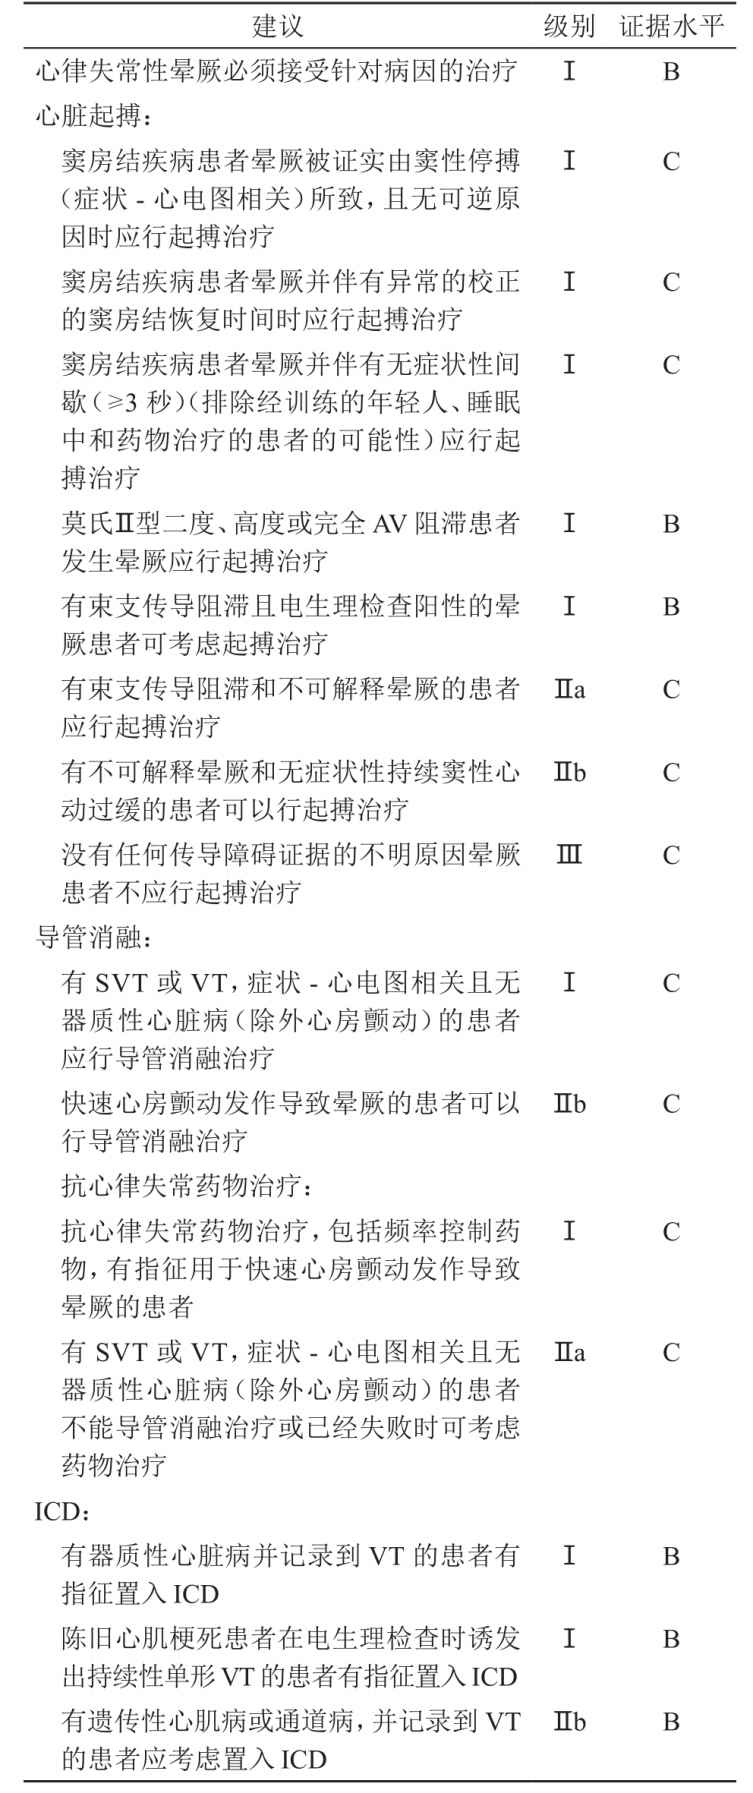
\includegraphics[width=3.29167in,height=7.86458in]{./images/Image00031.jpg}
\end{table}

\begin{table}[htbp]
\centering
\caption{SCD高危晕厥患者ICD适应证}
\label{tab4-14}
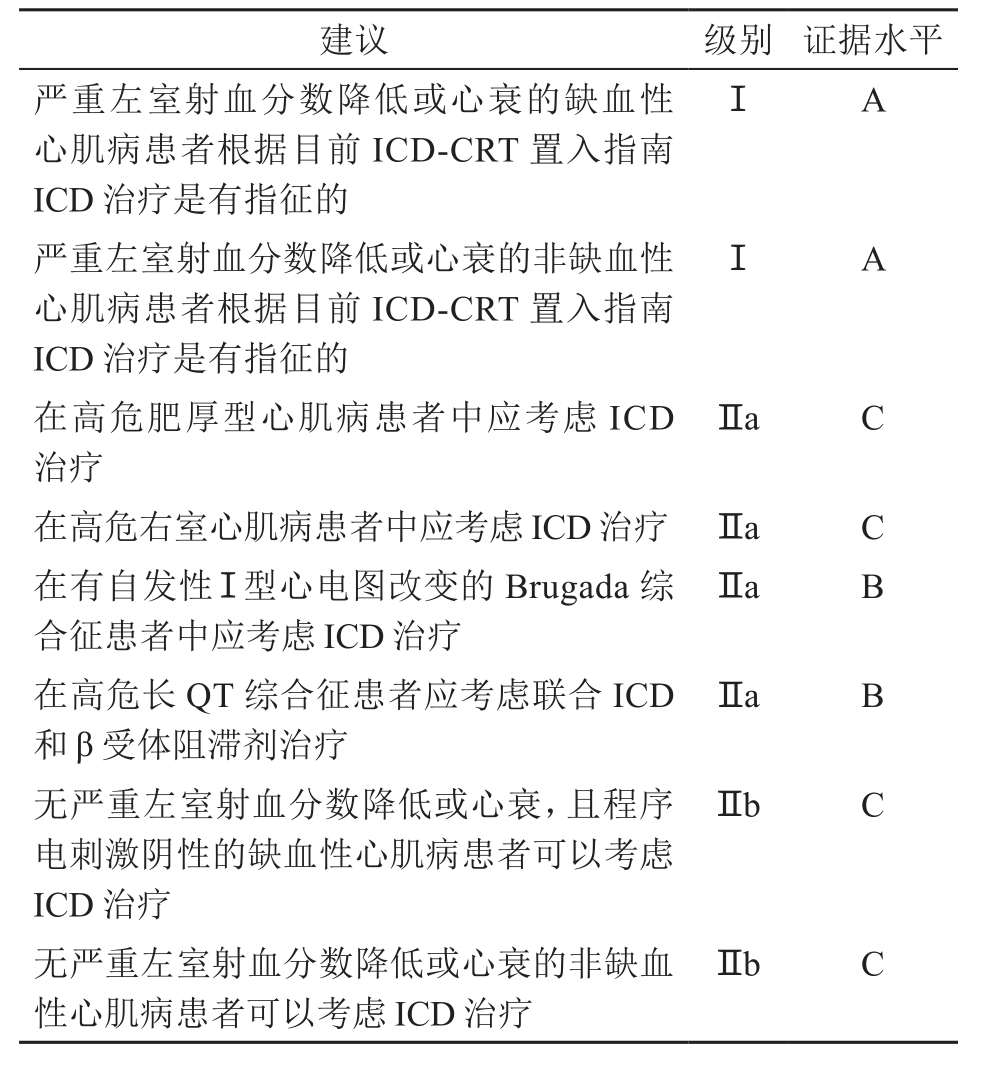
\includegraphics[width=3.3125in,height=3.55208in]{./images/Image00032.jpg}
\end{table}

\paragraph{特殊人群晕厥的处理}

\hypertarget{text00014.htmlux5cux23CHP1-4-4-1-5-1}{}
(1) 老年人晕厥:

老年人最常见的晕厥原因是OH、反射性晕厥,特别是颈动脉窦过敏和心律失常。一个患者可能有不同的机制共同作用,从而给诊断带来困难。与OH相关的住院治疗随着年龄的增加而增加,65~74岁是4.2\%,75岁以上为30.5\%。在有晕厥症状的患者之中,25\%是年龄相关的OH;其他OH主要是药物和特发性或继发性房颤所致。有OH的老年患者常有卧位收缩期高血压,并在接受多种药物治疗,给予OH药物治疗会加重卧位高血压,反之亦然。心脏抑制型颈动脉窦过敏是晕厥的原因,老年者高达20\%。血管减压型为主的颈动脉窦敏感同样常见,但是其在晕厥中的作用知之甚少。

对于老年人诊断检查和策略应注意:①老年人的OH常常具有重复性(特别是与药物或年龄相关)。因此,应反复进行OH评价,最好在早晨和(或)晕厥刚刚发生后进行。②对没有晕厥史者,即使颈动脉窦过敏不具特异性,颈动脉窦按摩检查也是特别重要的。③评价老年人反射性晕厥时,倾斜试验耐受性和安全性均很好。其阳性率与年轻人相仿,特别是在硝酸甘油激发后。④如果怀疑血压不稳定(如服药后或者餐后),24小时动态血压监测可能有帮助。⑤由于老年人心律失常发生频率高,对不明原因晕厥的老年人ILR特别有用。

\hypertarget{text00014.htmlux5cux23CHP1-4-4-1-5-2}{}
(2) 儿童晕厥:

对儿童晕厥的诊断评估与成人类似。反射性晕厥占病因学的绝大部分。但是在少数情况下,晕厥的发生是威胁生命的心律失常或心脏器质性异常所致。晕厥应该与癫痫和精神性假性晕厥鉴别,后者十分少见,但是是儿童TLOC的重要原因。

在幼童时期的两种特殊情况:①婴儿反射性晕厥发作(也叫做苍白屏气发作或反射性缺氧发作)是由短暂不愉快刺激导致的由迷走神经介导的心脏抑制所致。②窒息低氧性TLOC(发绀性呼吸停止)以哭闹时呼吸运动终止于呼气阶段为特征,从而导致发绀和通常所见的TLOC。

儿童倾斜试验的假阳性和假阴性率均较高,因此对于反射性晕厥的初步评估应持审慎态度。有报道对于健康少年儿童在静脉用药后进行倾斜试验时,先兆晕厥的比率非常高(40\%)。年轻患者首发晕厥可能为少见的、但是是威胁生命的疾病,如LQTS、Kearns-Sayre综合征(外眼肌麻痹和进行性心脏传导阻滞)、Brugada综合征、儿茶酚胺依赖性多形性VT、预激综合征、ARVC、肥厚型心肌病、肺动脉高压、心肌炎、先天性心脏病修补术后心律失常、冠状动脉异常起源。

对于具有下面情况的患儿可能提示有心脏性病因,应迅速进行心脏方面的评估:①家族史:年轻的SCD者<
30岁;家族性心脏病。②已知或可疑心脏病。③触发事件:噪音、惊吓、极端情感刺激。④运动时晕厥,包括游泳。⑤仰卧或者睡眠时无晕厥先兆,或晕厥前有胸痛或心悸。

儿童晕厥的治疗策略与成人相同。然而需要强调的是目前缺乏关于儿童反复晕厥良好设计的研究,因此药物和倾斜训练的有效性不能肯定。此外,尽管有血管迷走神经性晕厥以及长时间心脏停搏的证据,由于为一过性和良性晕厥,因此应避免安装起搏器。

总之,对儿童晕厥评估要点有几方面:①儿童期晕厥常见,绝大部分源于反射机制,很少部分是源于威胁生命的病因所致。②对良性和严重病因的鉴别主要依靠病史、体格检查和心电图。③对反射性晕厥年幼患者的治疗基石是教育并使之放心。

\hypertarget{text00014.htmlux5cux23CHP1-4-4-1-5-3}{}
(3) 驾车与晕厥:

随着轿车进入中国普通家庭,驾车与晕厥的问题显得重要起来。但是,调查显示,在有晕厥病史的患者中,交通事故的发生率低于普通人群。晕厥患者驾驶的建议见表\ref{tab4-15}。

\begin{table}[htbp]
\begin{center}
\caption{晕厥患者驾驶的建议}
\label{tab4-15}
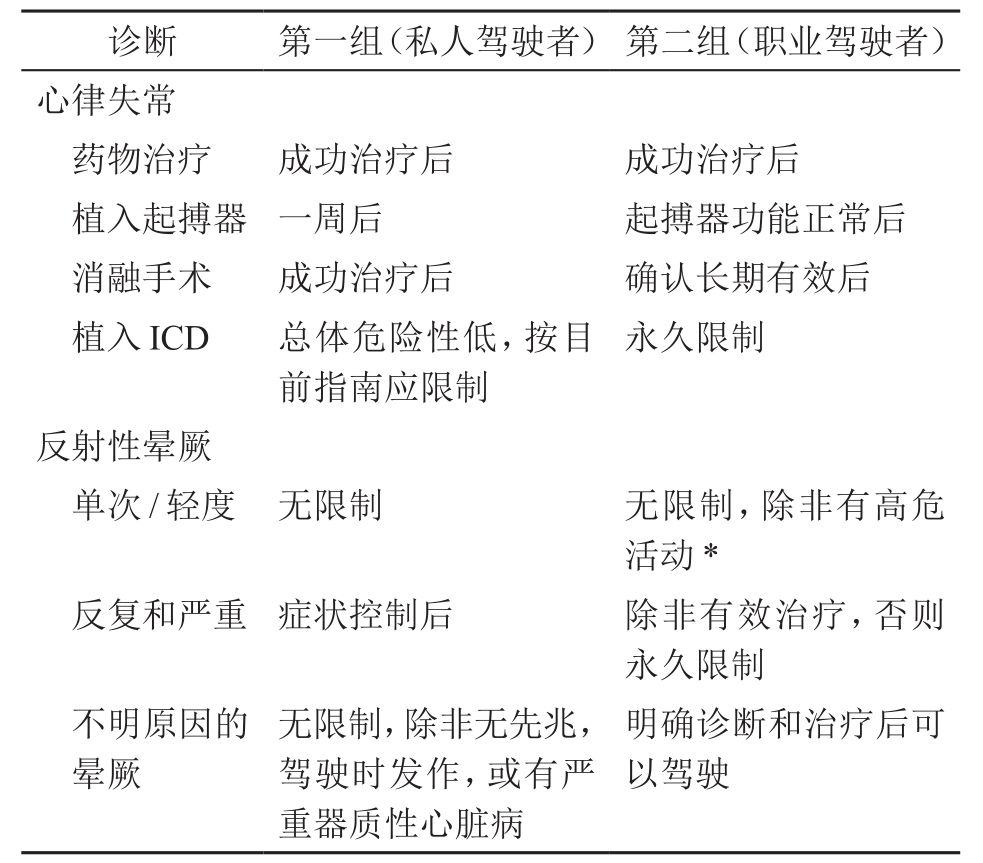
\includegraphics[width=3.27083in,height=2.86458in]{./images/Image00033.jpg}
\end{center}

{\small
注:第一组(私人驾驶者):驾驶摩托,小汽车或其他小型车辆,没有拖车;第二组(职业驾驶者):驾驶3.5吨以上汽车,除驾驶员外8座以上客车;出租车,救护车,介于私人与职业间车辆以及地方法规规定的车辆;

*:神经介导的晕厥严重且发作频繁,或正在从事高危活动;或者是复发或不可预测的高危患者
}
\end{table}

\subsection{预后}

晕厥的预后主要取决于两方面:①死亡风险及致命性事件:器质性心脏病及原发性电生理疾病是心源性猝死及晕厥患者总体死亡率的高危因素;合并联合病变的直立性低血压患者与普通人群相比,其死亡风险增加2倍;年轻且无器质性或电生理异常性心脏病的反射性晕厥患者,预后较好。大多数预后不良或死亡的患者多与基础疾病而非晕厥本身的严重程度有关。②晕厥复发及其危害:晕厥发生的次数是预测其复发的最佳指标,如诊断不明、低风险及年龄>
40岁、曾有1~2次晕厥发作史者,其复发率分别为15\%(1年内)和20\%(2年内);有3次发作史者,其复发率分别为36\%(1年内)和42\%(2年内)。


\hypertarget{text00015.htmlux5cux23CHP1-4-6}{}
参 考 文 献

Moya A,Sutton R,Ammimti F,et al. Guidelines for the diagnosis and
management of syncope(version 2009):the Task Force for the Diagnosis
and Management of Syncope of the European Society of
Cardiology(ESC).Eur Heart J,2009,30:2631-2671.

\protect\hypertarget{text00016.html}{}{}

\chapter{抽搐与惊厥}

抽搐(tics)系指全身或局部骨骼肌群非自主抽动或强烈收缩。抽搐包括痫性发作(seizure)和非痫性发作。痫性发作是脑神经元突然过度放电引起的短暂脑功能失调,患者出现全身(四肢、躯干、颜面)骨骼肌非自主强直性(持续肌肉收缩)与阵挛性(断续肌肉收缩)抽搐,引起关节运动和强直,又称癫痫发作。全面性强直-阵挛性抽搐即为惊厥发作(convulsion),常为全身性、对称性,多伴有意识障碍。

癫痫(epilepsy)则特指慢性反复发作性短暂脑功能失调综合征,具有反复性和发作性两个基本特征。癫痫持续状态(status
epilepticus)是抽搐患者最严重的表现形式之一,是指一次癫痫发作持续时间较久(>
30分钟),或癫痫频繁发作,发作间歇期意识尚未完全恢复。但研究显示较短暂的癫痫发作(<
30分钟)也可导致神经功能受损,且一旦痫性发作超过5分钟,自发终止的可能性就不大,所以建议在急诊情况下如癫痫发作超过5分钟即考虑癫痫持续状态。快速评估和控制癫痫发作是本章讨论的重点,从气道保护、神经功能稳定和寻找可能病因等三个方面积极应对,以减少其致残和死亡率。

\subsection{病因与发病机制}

抽搐的表现形式多样,主要分痫性发作和非痫性发作,前者有惊厥(全面性强直-阵挛发作)、强直性抽搐、肌阵挛发作、失神发作、自动症(automatism)等,后者见于低血钙手足抽搦、假性癫痫发作(如癔症性抽搐)等,因此其病因和发病机制非常复杂。

\subsubsection{病因}

\paragraph{癫痫和癫痫综合征}

具有特征性临床症状和脑电异常,但病因不清楚的癫痫发作,临床上倾向于基因突变和某些先天性因素所致,有明显遗传倾向;在患者神经系统中目前尚未发现有足以引起人类癫痫发作的器质性损伤或生化异常。

\paragraph{症状性癫痫}

各种明确或可能的中枢神经系统病变所致,如脑外伤、围产期损伤、脑血管病、肿瘤、中枢神经系统感染、寄生虫、遗传代谢性疾病(如低血糖)、神经系统变应性疾病、狼疮脑病等。

\paragraph{状态关联性癫痫发作}

患者癫痫发作与一些特殊状态有关,如高热、缺氧、内分泌和电解质异常(低血糖、低钠血症、高渗透压、尿毒症、肝功能衰竭)、药物与毒物、酒精和阿片类物质戒断、过度饮水、睡眠剥夺等。正常人(脑结构和功能正常)在上述特殊状态下也可出现癫痫发作,但一旦去除相关状态即不再出现癫痫发作。

\paragraph{隐源性癫痫发作}

临床表现提示症状性癫痫发作,但无特定的临床和脑电图特征,也未找到明确的病因。

上面所列主要是痫性发作抽搐的病因分类,为避免分类混乱,尚未包括非痫性发作抽搐相关病因。另外还要注意抽搐与晕厥、过度通气综合征、偏头痛、发作性睡病及各种不自主动作(如震颤、舞蹈动作、手足徐动、扭转痉挛、肌痉挛等)间的鉴别。

\subsubsection{发病机制}

抽搐的发生机制极为复杂,至今仍未阐明。目前脑组织的生理、生化方面的研究显示,抽搐发作主要机制是由大脑运动神经元的异常放电致脑功能短暂失调。该异常放电主要是神经元膜电位的不稳定引起,可由代谢、营养、皮质病变等激发,并与遗传、免疫、精神因素及微量元素等有关。具体来说,根据引起肌肉异常收缩的电兴奋信号的来源不同,可分为以下两类机制:

\paragraph{大脑功能的短暂性失调}

这是脑内神经元过度同步化放电的结果,当异常的电兴奋信号传至肌肉时,则引起广泛肌群的强烈收缩而形成抽搐。在正常情况下,脑内对神经元的过度放电及由此形成过度同步化,均有一定控制作用,即构成所谓抽搐阈。许多脑部病变或全身性疾病可通过破坏脑的控制作用,使抽搐阈下降,甚至引起抽搐。①神经元异常放电及其扩布:颅内外许多疾病,可通过不同途径影响膜电位的稳定,有直接引起膜电位降低(如低钠血症),使神经元更易去极化而产生动作电位(兴奋阈下降);间接通过影响能量代谢或能量缺乏,导致膜电位下降;神经元膜的通透性增高,使细胞外钠流入细胞内,而细胞内钾外流,因而膜电位及兴奋阈降低。②神经递质与突触传递的改变:中枢神经系统某些神经元的轴突于突触点释放抑制性递质,对神经元的过度放电及同步化也起一定控制作用。当兴奋性神经递质过多(如有机磷中毒时乙酰胆碱积聚过多)或抑制性神经递质过少(如维生素B\textsubscript{6}
缺乏时,由于谷氨酸脱羧酶的辅酶缺乏使谷氨酸转化成抑制性递质的γ-氨基丁酸减少)均可导致抽搐。③抑制系统通路受阻断:脑内有些神经元组成广泛的抑制系统,有控制神经元过度放电的作用。脑部病变除了直接损害神经元膜或通过影响脑血液供应外,也可能阻断抑制系统,使神经元容易过度兴奋。④网状结构的促去同化系统功能降低:脑干神经元放电同步化系统与网状结构的促去同化系统之间的平衡,对控制神经元的过度放电及同步化起相当的作用。

\paragraph{非大脑功能的障碍}

引起肌肉异常收缩的电兴奋信号来源于下运动神经元,主要是脊髓的运动神经元或周围运动神经元。如破伤风杆菌外毒素选择性作用于中枢神经系统(主要是脊髓、脑干的下运动神经元)的突触,使其肿胀而发生功能障碍;马钱子碱中毒引起脊髓前角细胞过度兴奋,发生类似破伤风的抽搐;各种原因的低钙血症,除了使神经元膜通透性增高外,也常由于下运动神经元的轴突(周围神经)和肌膜对钠离子的通透性增加而兴奋性升高,引起手足搐搦。

\subsubsection{儿童惊厥发病机制}

儿童惊厥(6岁以下)发生率是成人的10~15倍,儿童惊厥的发病机制有其特殊性。婴幼儿大脑皮质功能未完善/抑制差、兴奋易扩散、神经髓鞘未完全形成、神经传导分化不全、冲动易泛化、血-脑脊液屏障不良、毒物易渗入脑组织及水电解质代谢不稳定等因素是导致儿童惊厥高发生率的主要原因。相对成人而言,短暂性脑功能失调对小儿神经系统发育影响更大,一次惊厥对近记忆的一过性影响与脑震荡所致的损伤相当,而惊厥持续状态可产生严重不可逆脑损伤,小儿惊厥30分钟以上就可产生神经元缺血病变,影响小儿智力和健康。通常成人惊厥超过6小时才产生类似变化。

\subsection{诊断思路}

抽搐并不是单一疾病,而是许多疾病的严重临床表现或主要征象。因此,在诊断过程中,应综合分析各方面资料,才能明确其发生的原因。

\subsubsection{抽搐的诊断}

\hypertarget{text00016.htmlux5cux23CHP1-5-2-1-1}{}
(一) 病史

不同疾病所致的抽搐 ,其临床表现不尽相同,故详细收集病史是非常重要的。

\paragraph{明确抽搐类型}

依抽搐的形式,可分为以下两种:①痫性发作(癫痫发作);②非痫性发作。前者(尤其是全面性强直-阵挛发作,即惊厥发作)需要急诊医师快速评估和保护气道、控制癫痫发作,并积极寻找病因。而非痫性发作抽搐虽然不似前者致命,但抽搐的控制更加困难,临床重点是寻找可能病因。判断癫痫发作最重要的依据是患者的病史,如先兆症状、发作时状态及发作后意识模糊等,而不是依靠神经系统查体和实验室检查。患者发作后意识模糊状态高度提示癫痫发作。

\paragraph{了解基础疾病和用药史}

对诊断有重要参考价值。如反复发作常提示癫痫,新近发生的癫痫发作通常由于原发性神经疾病和系统性疾病或代谢紊乱所致,有外伤、感染以及内脏器官基础疾病史者提示可能为症状性癫痫。还须详细了解用药史和饮酒史,尤其是抗癫痫药物使用情况。

\paragraph{伴随症状}

对病因诊断有相当意义。

\hypertarget{text00016.htmlux5cux23CHP1-5-2-1-1-3-1}{}
(1) 症状性癫痫发作:

①颅内疾病时可伴有头痛、发热等;②阿-斯综合征抽搐时伴有心搏停止、心音及脉搏消失;③低血糖所致抽搐前多有乏力、饥饿、出汗,发作时伴有心动过速、血压升高、瞳孔散大;④子痫者伴有头痛、眼花、呕吐,可有高血压、水肿和蛋白尿;⑤嗜铬细胞瘤时伴有心跳快、气促、出汗、面色及四肢苍白、发冷、头痛、血压急剧升高、瞳孔散大;⑥尿毒症患者伴有氮质血症和酸中毒表现。

\hypertarget{text00016.htmlux5cux23CHP1-5-2-1-1-3-2}{}
(2) 低血钙性手足搐搦症:

①甲状旁腺功能减退症患者可伴有哮喘,易激动、焦虑等精神症状,皮肤粗糙,头发脱落,牙齿发育不良;②肠源性手足搐搦症患者伴有慢性腹泻;③肾病性手足搐搦症患者伴有代谢性酸中毒表现;④假性甲状旁腺功能减退症患者伴有先天畸形如矮胖、圆脸、短指。

\hypertarget{text00016.htmlux5cux23CHP1-5-2-1-1-3-3}{}
(3) 血钙正常性碱中毒性手足搐搦症:

伴有引起碱中毒的症状,如过度换气,大量呕吐或服用大量碱性药物。

\hypertarget{text00016.htmlux5cux23CHP1-5-2-1-2}{}
(二) 体格检查

导致抽搐病因众多 ,常涉及临床各科,详细系统地体检十分重要。通常包括:

\paragraph{系统查体}

重点是生命体征和有无创伤表现。但几乎体内各重要内脏器官的疾病均可引起抽搐,故须按系统进行检查。如心音及脉搏消失、血压下降或测不到,或严重心律失常,要考虑心源性抽搐;苦笑面容、牙关紧闭、角弓反张者要考虑破伤风;怀疑手足抽搦症时要查:①Chvostek征:以中指轻扣耳前面神经,可引起同侧面肌抽搐;②Trousseau征:以血压计袖带缠绕一侧上臂,打气至舒张压与收缩压之间,维持3分钟,可引起该侧手的搐搦。

\paragraph{神经和精神科查体}

有助于致抽搐病变的定性与定位。重点注意瞳孔反射、病理征、局灶神经体征、眼底情况。

\hypertarget{text00016.htmlux5cux23CHP1-5-2-1-3}{}
(三) 辅助检查

根据病史
、体检所提供的线索,选择辅助检查项目。①全身性疾病:应选择相应的检查。除了血尿粪常规外,有心电图、血液生化(血糖、尿素氮、电解质等)、血气分析、肝肾功能、内分泌功能测定、毒物分析等。②神经系统疾病:根据临床提示的病变部位和性质,选择相应的辅助检查。如脑电图、肌电图、脑脊液、神经影像学检查(头颅CT、MRI、MRA)等,近年来PET等功能影像学检查手段越来越多地被用于抽搐的病因诊断,它可实现脑局部代谢变化,辅助癫痫灶定位。

\subsubsection{抽搐的病因判断}

所有抽搐患者均应结合上述资料尽可能做出病因诊断,如为首次发作,首先须排除各种疾病引起的症状性发作,寻找可逆因素(如低血糖、低钠血症、低钙血症、药物过量等)。临床上还可根据抽搐时是否伴有意识障碍,可将抽搐分为两大类:

\hypertarget{text00016.htmlux5cux23CHP1-5-2-2-1}{}
(一) 伴意识障碍性抽搐

\paragraph{大脑器质性损害性抽搐}

其特点为:①抽搐为阵挛性和(或)强直性;②意识障碍较重,持续时间长,且多伴有瞳孔散大、大小便失禁、面色青紫等表现,多数有颅内高压表现;③脑脊液检查常有异常发现,脑电图、CT、MRI等检查有助于诊断。

\paragraph{大脑非器质性损害性抽搐}

其特点有:①意识障碍可轻可重,多数为短暂性昏迷,约在数秒至数十秒内自行恢复;②全身性疾病的表现往往比神经系统表现更明显;③无明确的神经系统定位体征;④脑脊液检查和脑电图检查多正常。

\hypertarget{text00016.htmlux5cux23CHP1-5-2-2-2}{}
(二) 不伴意识障碍性抽搐

可分为神经肌肉兴奋性增加(见于低血钙或低血镁、破伤风或马钱子碱中毒)和神经肌肉兴奋性正常(见于药物戒断反应、癔症性抽搐)两类,但以电解质紊乱(如低血钙、低血镁等)所致者较为常见。此类抽搐的特点是呈疼痛性、紧张性肌收缩,常伴有感觉异常。根据病史和临床表现常可确定这类抽搐的病因。如诊断有困难时,可测定血钙与血镁。在紧急情况下,可先静注10\%葡萄糖酸钙10ml,无效时可再静注25\%硫酸镁5~10ml。这样既有鉴别诊断的意义,又有治疗作用。

\subsubsection{临床常见抽搐}

\paragraph{癫痫发作(痫性发作)}

患者出现全身骨骼肌非自主强直性与阵挛性抽搐,引起关节运动和强直,伴或不伴意识障碍。根据临床表现可分为:①部分发作(局灶发作):单纯部分性发作(发作时无意识障碍)、复杂部分性发作(有不同程度意识障碍);②全面性发作:全面性强直-阵挛发作(即癫痫大发作,俗称惊厥,部分患者发作前有先兆,分强直期、阵挛期和痉挛后期)、强直性发作、阵挛性发作、肌阵挛发作、失神发作、失张力性发作等。

分类颇显繁杂,急诊临床重点是识别:是否是癫痫发作?是全面性发作吗?是癫痫持续状态吗?由于癫痫持续状态期间脑神经元能耗骤增,脑内pH下降,加之全身性缺氧,肌肉强烈而持久性收缩,酸性代谢产物增加,可导致脑缺氧、脑水肿甚至脑疝形成。持续状态时需要紧急保护气道、控制癫痫发作(稳定神经功能)和确定病因。

\paragraph{手足搐搦症}

以疼痛性、紧张性肌肉收缩为特征,多伴有感觉异常,见于各种原因所致的低钙血症和低镁血症。表现为间歇发生的双侧强直性痉挛,上肢较显著,尤其是在手部肌肉,呈典型的:“助产手”,即手指伸直内收,拇指对掌内收,掌指关节和腕部屈曲;常有肘伸直和外旋。下肢受累时,呈现足趾和踝部屈曲,膝伸直。严重时可有口、眼轮匝肌的痉挛。发作时意识清,Chvostek征和Trousseau征阳性。

\paragraph{破伤风}

破伤风杆菌外毒素-破伤风痉挛毒素可阻断脊髓的抑制反射,脊髓前角运动神经元兴奋性增高,同时也使脑干广泛脱抑,导致肌痉挛、肌强直,表现为张口困难、牙关紧闭、腹肌僵硬、角弓反张。肌强直的特点是在抽搐间歇期仍存在,肌抽搐可为自发性,亦可因外界刺激而引起,面肌强直和痉挛形成苦笑面容,咽肌和膈肌受累导致饮水困难和呛咳。破伤风的抽搐虽可十分严重,但神志清楚。外伤史有助于疾病的诊断。

\paragraph{癔症性抽搐}

属一种功能性动作异常。患者多为年轻女性,在精神因素刺激下发作,表现为突然倒下,全身僵直、牙关紧闭、双手握拳,其后不规则的手足舞动,常杂以捶胸顿足、哭笑叫骂等情感反应,发作持续数分钟至数小时。其特点是:①抽搐动作杂乱,无规律可循,不指向神经系统的某一定位损害;②无瞳孔变化和病理反射;③常伴有流泪、过度呼吸、眼活动频繁和眨眼过度;④无舌头损伤及大小便失禁;⑤发作时脑电图正常;⑥暗示或强刺激可终止其发作。

\paragraph{发热惊厥}

惊厥发作的典型临床表现是意识突然丧失,同时急骤发生全身性或局限性、强直性或阵挛性面部、四肢肌肉抽搐,多伴有双眼上翻、凝视或斜视。最常见于幼儿,发病多在6个月至6岁之间,以3岁以前小儿多见。最常见于上呼吸道感染、扁桃腺炎,少数见于消化道感染或出疹性疾病,约一半患儿有家族史,提示同遗传因素有关。惊厥的发生常与发热相关,但热度高低并不与之呈正相关。发作形式多为单次,全身性强直、阵挛性发作,持续时间在30秒钟以内,一般不超过10分钟,脑电图有节律变慢或枕区高幅慢波,在退热后1周内消失。可能每年有一至数次同样发作,但若无脑损害征象,并不导致癫痫。

\paragraph{中毒性抽搐}

最常见于急性中毒。其发生抽搐的主要机制:①直接作用于脑或脊髓,使神经元的兴奋性增高而发生抽搐。大多是药物的过量,如戊四氮、贝美格(美解眠)、樟脑、印防己毒素、阿托品、麦角胺、丙米嗪、氯丙嗪、白果等;②中毒后缺氧或毒物作用,引起脑代谢及血循环障碍,形成脑水肿。见于各种重金属、有机化合物、某些药物和食物的急性重度中毒。临床多呈全身性肌强直阵挛性发作,少数也可呈局限性抽搐,有的可发展为癫痫状态。常合并其他中毒表现。马钱子碱(士的宁)中毒的临床表现类似破伤风,仅在抽搐间隙无持续性的肌痉挛。

\paragraph{心源性抽搐}

是指各种原因引起心排出量锐减或心脏停搏,使脑供血短期内急剧下降所致的突然意识丧失及抽搐,也称昏厥性抽搐。常见于严重心律失常、心排血受阻的心脏病或某些先天性心脏病、心肌缺血、颈动脉窦过敏、血管抑制性昏厥、直立性低血压等。其抽搐时间多在10秒钟内,较少超过15秒钟,先有强直,躯体后仰,双手握拳,接着双上肢至面部阵挛性痉挛,伴有意识丧失,瞳孔散大、流涎,偶有大小便失禁。发作时心音及脉搏消失,血压明显下降或测不到。脑电图在抽搐时呈电位低平,其后为慢波,随意识恢复后逐渐正常。

\paragraph{急性颅脑疾病相关抽搐}

颅内感染、颅脑损伤、急性脑血管病是导致症状性癫痫发作的主要因素。抽搐多为痫性发作,且多与病变程度相平衡,有的随着颅脑病变的加剧抽搐频繁、加剧,甚至发展为癫痫持续状态。抽搐仅是临床表现之一,大多还有脑局灶或弥散损害的征象,如头痛、呕吐、精神异常、偏瘫、失语、意识障碍、脑膜刺激征等表现。脑脊液检查及CT、MRI等检查可有相应的阳性发现。

\paragraph{药物戒断反应}

长期连续服用安眠药,主要是巴比妥类安眠药患者,常产生药物依赖性甚至成瘾,在突然停药后可引起严重戒断反应,表现为异常兴奋,焦虑不安、躁动甚至发生四肢抽搐或强直性惊厥。阿片类药物的戒断反应较安眠药更严重而持久。处理主要是对症治疗,并逐渐停药。

\paragraph{代谢、内分泌异常所致的抽搐}

许多代谢、内分泌疾患,可因电解质紊乱,能量供应障碍等,干扰了神经细胞膜的稳定性,而出现抽搐,同时有明显代谢、内分泌异常的临床表现。如各种疾病所致的低钙血症、低钠血症、低镁血症、碱中毒、低血糖症(血糖<
2mmol/L)等,均可致抽搐。

\subsection{处理原则}

\subsubsection{急诊处理思路}

\paragraph{他人发现患者抽搐、晕厥、昏迷?}

急诊抽搐患者往往是被他人送来急诊就诊,而旁观者很难分别是抽搐,还是晕厥或昏迷,这时急诊医师不要仓促下结论患者是癫痫发作,具体分析思路见图\ref{fig5-1}。

\paragraph{考虑癫痫发作的分析和处理思路}

在急诊抽搐患者处理的难点正是如何判断是否是癫痫发作,可通过以下线索来分析判断:强直-阵挛性运动病史、大小便失禁、发作后意识模糊、舌体咬伤等。在急诊如经过初始评估考虑患者为癫痫发作时,临床分析思路参考图\ref{fig5-2}。但患者的处理依然优先要考虑初始评估、稳定(保护气道)、神经功能稳定(控制癫痫发作)、寻找病因这一处理流程。

\subsubsection{保护气道}

首先应将患者置于安全处,解开衣扣,去除义齿,清除口腔异物,保持呼吸道通畅。有意识障碍者,将身体或头须转向一侧,以利口腔分泌物流出,防止吸入肺内致窒息或肺炎。分泌物较多者,准备好负压吸引器,随时吸痰。必要时给氧,气管切开或气管插管给予人工呼吸,维持正常的通气功能。

\subsubsection{快速评估和稳定}

重症病例应进行血压、心电图和脉搏氧饱和度等监测,急查血电解质和动脉血气,并予吸氧,建立静脉通路。若有异常发现,应及时处理。如给予抗抽搐药物不能终止癫痫发作,需作好气管插管准备。

低血糖是最常见引起痫性发作的代谢性因素,另一方面,要注意长时间抽搐也可致低血糖,低血糖症者,应给予50\%葡萄糖50m1,静脉推注(5分钟内);有糖尿病高血糖者,应给予胰岛素治疗。

疑有营养不良症者,应给予维生素B\textsubscript{l}
l00mg肌肉注射或静脉注射;怀疑异烟肼过量者应用维生素B\textsubscript{6}
;有低血钙症者,应给予10\%葡萄糖酸钙10ml或10\%氯化钙10m1,缓慢静脉注射(5分钟以上),必要时重复给药,但24小时给予的总钙量,一般不超过25mmol。

\begin{figure}[!htbp]
 \centering
 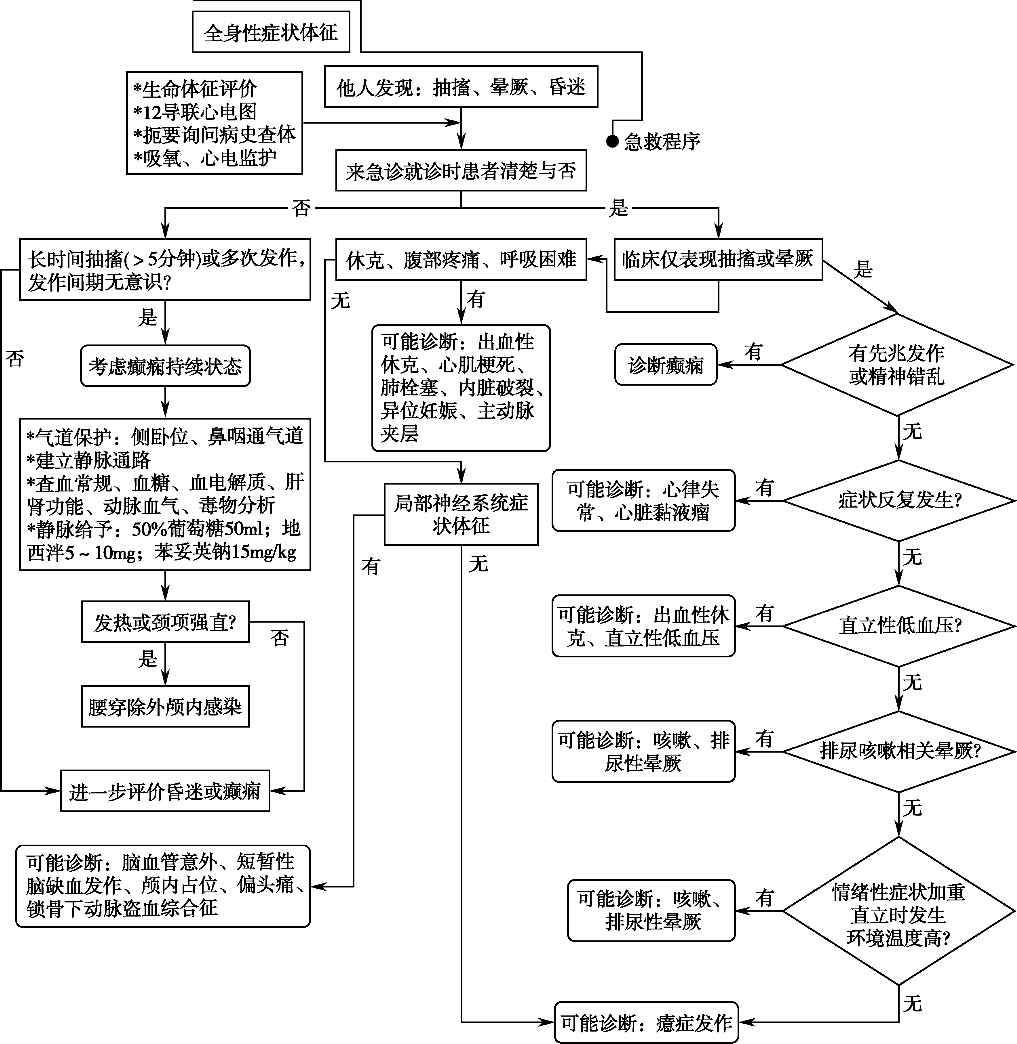
\includegraphics[width=5.88542in,height=6.04167in]{./images/Image00034.jpg}
 \captionsetup{justification=centering}
 \caption{他人发现抽搐、晕厥或昏迷患者分析思路}
 \label{fig5-1}
  \end{figure} 

\begin{figure}[!htbp]
 \centering
 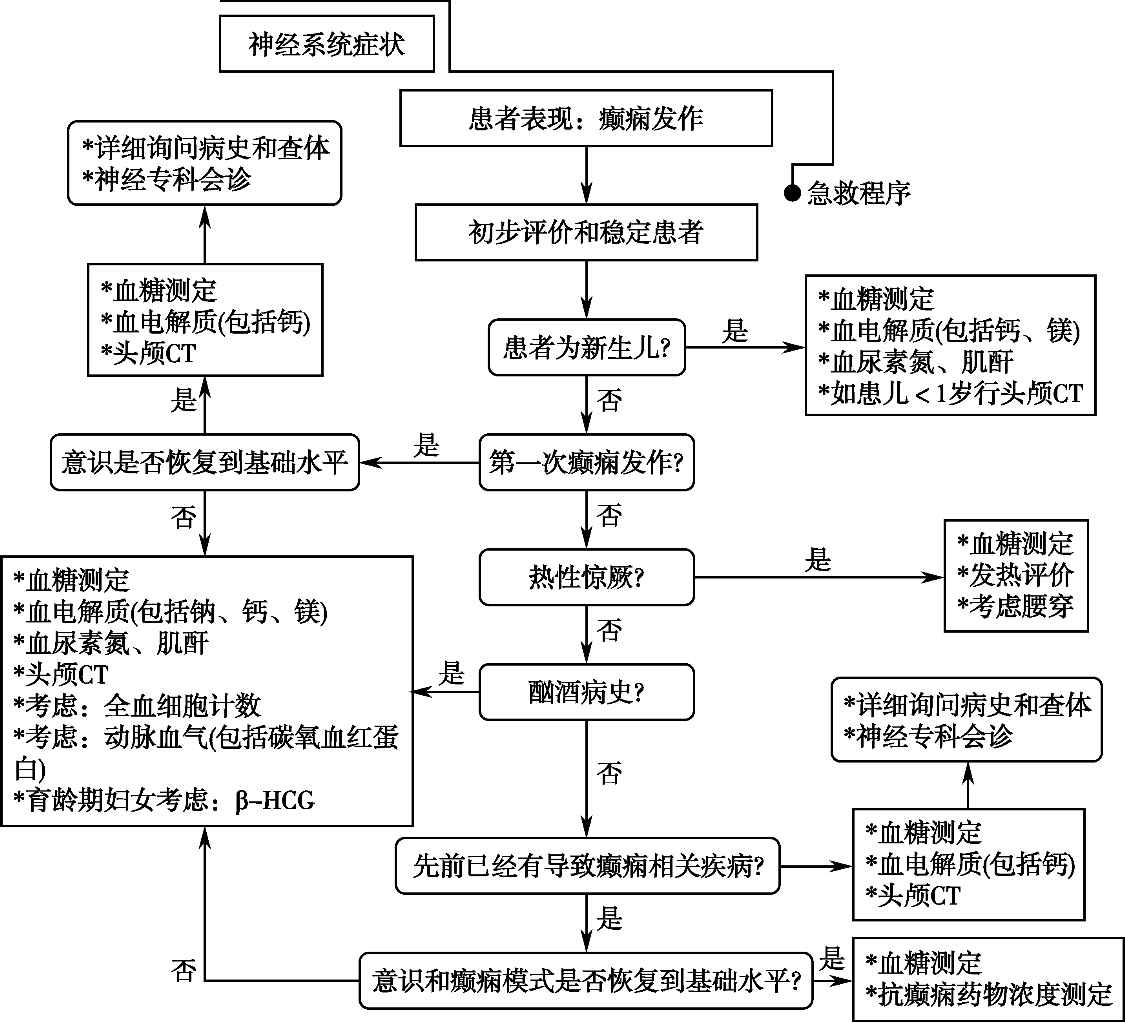
\includegraphics[width=4.77083in,height=4.34375in]{./images/Image00035.jpg}
 \captionsetup{justification=centering}
 \caption{癫痫发作的分析和处理思路}
 \label{fig5-2}
  \end{figure} 

\subsubsection{控制抽搐发作}

一旦确定是全身强直-阵挛性发作(癫痫大发作)或癫痫持续状态,及时控制抽搐是临床治疗的关键。癫痫持续状态处理流程见图\ref{fig5-3},有很强的时间紧迫性,目标是在神经功能受损前控制癫痫发作(理论上是在20分钟至1小时内控制抽搐发作)。应优先选择抗惊厥作用强、吸收快、分布半衰期长、排除半衰期短、无心肺和意识抑制作用,能肌肉注射、静脉注射和毒副作用低的药物。癫痫持续状态的药物治疗应根据患者的个体情况及时适度地应用,力争在最短的时间内终止癫痫发作,然后给予维持治疗。抽搐时切记勿强行固定四肢(否则易导致骨折、脱臼),也不要在抽搐时往患者嘴里塞牙垫、毛巾等物。抽搐停止后应加强监护,以防自伤、误伤、伤人、毁物等。

\paragraph{地西泮(安定)}

为一线控制癫痫发作药物,适用于各年龄段。见效快,半衰期短(0.5~4小时)。成人首次剂量10~20mg,按1~5mg/min缓慢静脉注射,有效而复发者,30分钟后可重复应用,或在首次用药后将安定20~40mg加入10\%葡萄糖液100~250ml中缓慢静滴,10~20mg/h,用于维持疗效,视发作情况控制滴注速度和剂量,24小时总剂量不宜超过120mg(注:在控制癫痫发作时,地西泮剂量理论上来说没有上限)。无论地西泮的疗效如何,宜与苯妥英钠或苯巴比妥合用,预防抽搐再次发作。

儿童地西泮剂量每次0.25~0.5mg/kg静推,速度1mg/min,婴儿不超过2mg/次,幼儿不超过5mg/次。5~10岁儿童1mg/岁,儿童一次用量不超过10mg。新生儿及婴儿亦可用地西泮,每次0.5~1mg/kg肛管给药。

其他苯二氮{}
类制剂亦可选用,如劳拉西泮(氯羟安定),与地西泮相比抗惊厥作用强5倍,作用时间长3~4倍,半衰期12~16小时。静脉注射2~5mg/次(0.1mg/kg,速度2mg/min),80\%以上病例可在2~3分钟内终止发作,特别推荐在酒精戒断相关癫痫发作患者中使用。最新研究显示静脉注射劳拉西泮在控制抽搐和预防复发方面均优于地西泮。氯硝西泮抗惊厥作用是地西泮的5倍,半衰期22~32小时,静脉注射1~4mg/次,60\%病例可控制发作24小时。

如果尚未给患者建立静脉通路,地西泮可以通过直肠、气管套管内、骨髓腔内等途径给药。苯二氮{}
类药物有呼吸抑制、心动过缓和低血压、酸中毒等副作用,应用时需随时评估气道,脉搏氧饱和度降至90\%以下或呛咳作呕反射消失者,应考虑予气管插管。

\paragraph{苯妥英钠}

控制成人癫痫发作二线治疗药物,无呼吸抑制,静脉给药能迅速达到脑内有效浓度。常用为150~250mg/次(20mg/kg),生理盐水溶解,缓慢静脉注射(1分钟小于50mg),半小时后可重复给药(100~150mg)。严重病例可加大用药剂量。儿童用量为250mg/m\textsuperscript{2}
。因为有低血压和心律失常等副作用,胃肠外给药速度不要过快,用药期间应密切观察,或行心电图和血压监测。

\paragraph{苯巴比妥钠}

控制成人癫痫发作三线治疗药物。若足量的苯妥英钠仍不能控制抽搐发作,应立即给予苯巴比妥钠治疗。按10mg/kg静脉缓慢注射(50~100mg/min),直至发作停止,可再追加50mg,剩余部分可行肌肉注射。呼吸抑制和低血压是其常见副作用,用药前应准备气管插管和人工辅助呼吸通气。注射过程中需密切观察呼吸情况,如有抑制呼吸现象应立即停止注射,并作人工辅助通气。注意对儿童来说苯巴比妥钠是二线药物,而苯妥英钠是三线药物。

\begin{figure}[!htbp]
 \begin{center}
 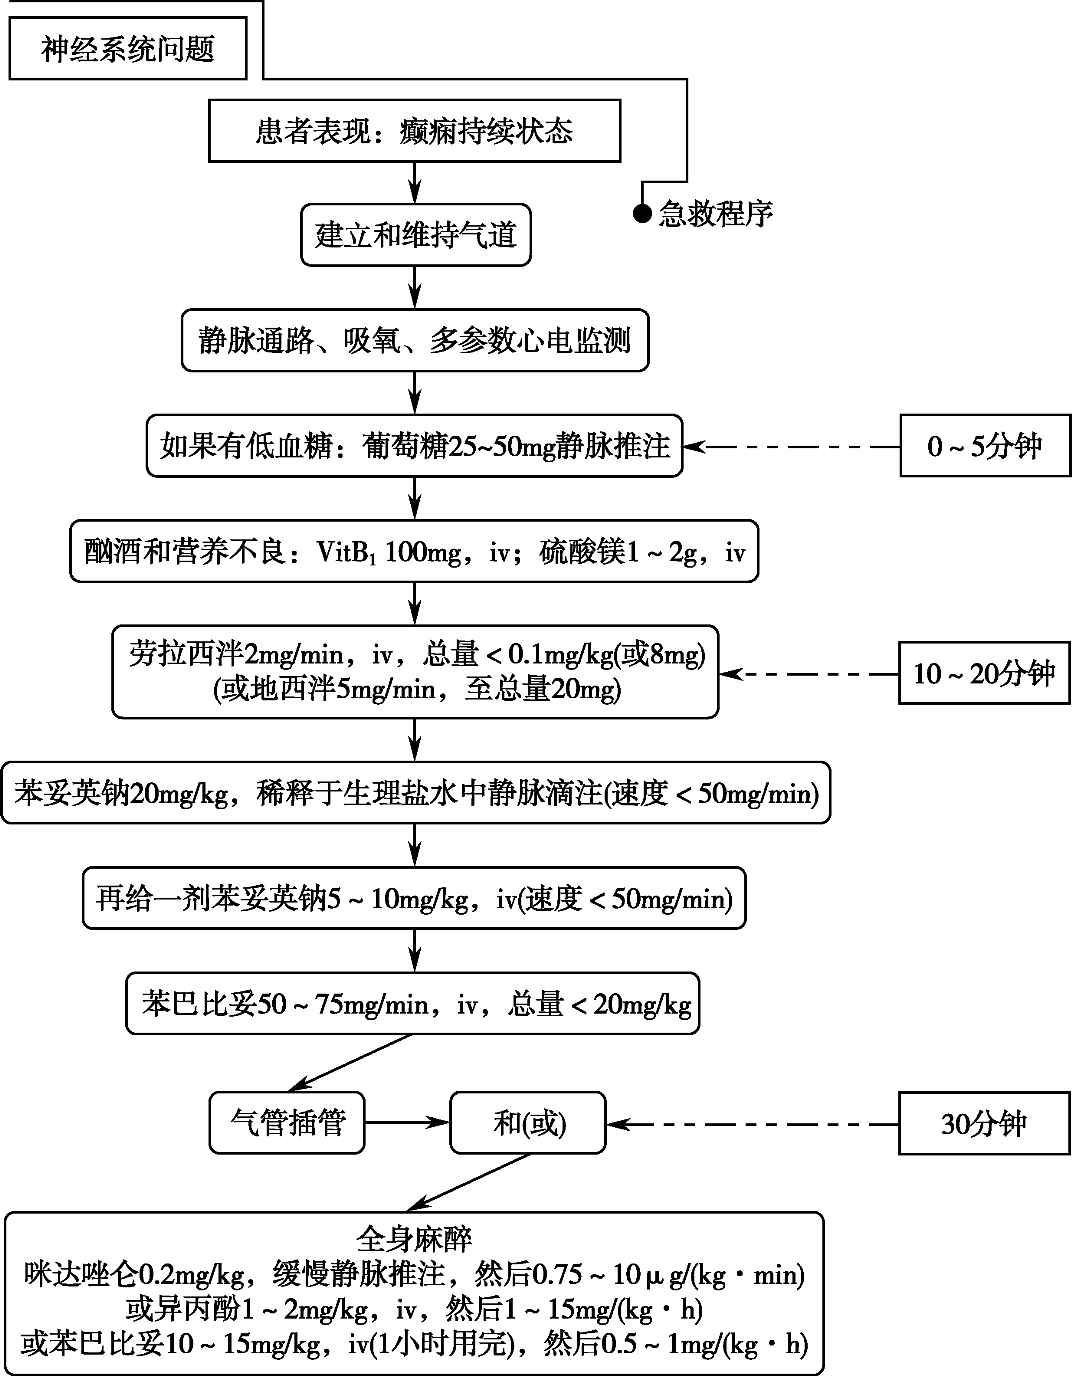
\includegraphics[width=4.11458in,height=5.28125in]{./images/Image00038.jpg}
 \captionsetup{justification=centering}
 \caption{癫痫持续状态处理路径}
 \label{fig5-3}
 \end{center}

 {\small
 注:苯巴比妥剂量在国内有限制:一次极量为0.3g,一日极量为0.5g
 }
 \end{figure} 

\paragraph{其他药物}

如上述治疗无效,应考虑请神经专科医师会诊,并试用下列药物:①丙戊酸:控制癫痫发作有效药物。推荐剂量是15~20mg/kg或600~1200mg/d,分2~3次口服,其临床安全性良好,但注意在肝功能不全患者中禁用。②副醛:成人8~10ml、儿童0.3ml/kg,用植物油稀释后保留灌肠。代谢性酸中毒、肺出血、心血管抑制和直肠炎等是常见的副作用,应注意观察。③利多卡因:成人用1\%的利多卡因10ml,以20mg/min速度匀速静注。可降低心输出量,有充血性心力衰竭和肝损害减量。④10\%水合氯醛:成人20~30ml、儿童0.3ml/kg保留灌肠。

\paragraph{全身麻醉}

处理仍无效者,可考虑收入ICU,静脉持续泵入咪达唑仑、丙泊酚等药控制癫痫发作,但其临床疗效有待进一步验证,也试用下列药物全身麻醉:①戊巴比妥:15mg/kg缓慢静脉注射,然后以0.5~1mg/(kg•h)维持。②硫喷妥钠:15mg/kg静脉缓慢推注,继以5mg/(kg•h)静脉注射维持。脑内的半衰期低于30分钟。③异戊巴比妥:200~1000mg静脉缓慢推注。

\subsubsection{病因治疗}

病因治疗是根本。如中毒性抽搐,应尽速彻底清除毒物和应用特效的解毒剂;急性感染性疾病所致者选用相应有效的抗生素,破伤风者须应用破伤风免疫球蛋白和抗生素(甲硝唑);高热惊厥,首先降温,使体温控制在38℃以下;低血糖发作应立即静注50\%葡萄糖液;水电解质平衡失调应分别纠正所缺少的钙、钠、镁;心源性抽搐者,应尽快建立有效循环,提高心排出量,治疗原发病;对肝肾功能衰竭者,改善并恢复其功能至关重要;颅内肿瘤、血肿、脓肿、脑寄生虫病及各种原因的脑水肿引起抽搐者,必须脱水降颅内压,必要时外科手术治疗。

\subsubsection{对症治疗}

癫痫持续状态l小时以上者,即有发生脑缺氧脑水肿的可能性,应酌情给予地塞米松、20\%甘露醇或利尿剂治疗,为了预防继发感染,应给予抗生素治疗。有高热者应给予降低过高体温处理。严重抽搐发作时,还可出现酸中毒、电解质紊乱、横纹肌溶解等并发症,进而又加重抽搐发作,甚至危及生命。临床上在控制癫痫发作的同时,应注意寻找并处理并发症。必须注意维持呼吸、循环、体温、水电解质平衡,保证供氧,供给充足热量,避免缺氧及缺血性脑损害。


\hypertarget{text00017.htmlux5cux23CHP1-5-4}{}
参 考 文 献

1. John Marx. Rosen's Emergency Medicine. 7th ed. Mosby,2009:113

2. Tintinalli JE. Emergency Medicine:A comprehensive study guide.6th
ed. McGraw-Hill,2004:1409

3. Rowland LP. Merritt's Neurology. 11th ed. Lippincott Williams
&Wilkins,2005:13

4. Pillow MT. Emergency Medicine. emedicine(http://emedicine.
medscape.com)updated Nov 9,2010

5. Huff JS. Emergency medicine clinics of North
America.2011,29(1):1-158

\protect\hypertarget{text00018.html}{}{}

\chapter{瘫 痪}

本章叙述的瘫痪(paralysis)是指随意肌收缩功能不全而言。其不完全障碍形成的肌力减退,属不完全性瘫痪;其完全障碍形成的随意肌收缩不能,属完全性瘫痪。本文叙述急性瘫痪的诊断与其处理原则。

\subsection{各型瘫痪的临床特征}

按病损部位不同,可将瘫痪分为肌源性、神经-肌接点性、下运动神经元性或上运动神经元性,其临床表现各具特征。现予分述如下:

\subsubsection{肌源性或神经-肌接点病损性瘫痪的临床特征}

肌源性瘫痪是指肌肉本身病变导致肌肉收缩障碍,从而引起程度不等的瘫痪而言。神经-肌接点病损性瘫痪是指神经-肌接点的递质因素或递质受体病变所引起的肌肉收缩无力而出现的瘫痪而言。

\paragraph{瘫痪分布}

大多对称,多以肢体近端为重,不符合神经支配规律。

\paragraph{肌束震颤}

通常没有。

\paragraph{肌肉萎缩}

随病程进展,出现病肌萎缩,但不出现于疾病的急性期。

\paragraph{牵张反射}

由于运动效应器病损,致紧张性牵张反射(表现为肌张力)与位相性牵张反射(表现为腱反射)均见降低。

\paragraph{病理反射}

病理反射是上运动神经元性瘫痪的特征,因此,通常不见于肌源性或神经-肌接点病损性瘫痪。

\paragraph{实验室检查}

肌细胞病变时出现血肌酶如肌酸磷酸激酶等升高;肌电图呈肌病性变;肌肉活检证实各种肌肉疾病的特征性改变。神经-肌接点病损性瘫痪时,通常血肌酶变动不明显,肌电图检查显示特征性改变。

\subsubsection{下运动神经元性瘫痪的临床特征}

\paragraph{瘫痪分布}

主要是小组肌肉或单块肌肉的瘫痪,其分布符合脊髄节段或周围神经支配的规律。

\paragraph{肌束震颤}

束颤是下运动神经元性瘫痪的特征之一,但是很少见于瘫痪的急性病期。随意肌失神经支配后,在其足板附近的肌膜上,烟碱型乙酰胆碱受体大量增生,以致血循环中存在着的小量乙酰胆碱,足以引起肌纤维的自发性收缩而在肌电图上显示为纤维颤动(纤颤)电位。纤颤电位通常见于骨骼肌失神经支配后1~3周。当整个肌束有类似变化时,就出现肉眼可见的束颤。在确认束颤与下运动神经元病变有关前,必须除外良性束颤与可能含有束颤的其他疾病如抗胆碱酯酶药物过量与电解质紊乱等。

\paragraph{肌肉萎缩}

通常始于失神经支配1~2周后。是其蛋白代谢呈负平衡的结果。

\paragraph{牵张反射}

由于反射通路受阻而致肌张力、腱反射均见减退。睡眠、昏迷或小脑病变时,也见牵张反射减退,诊断时应注意识别。

\paragraph{病理反射}

病理反射是上运动神经元性瘫痪的病征,不见于下运动神经元性瘫痪。

\paragraph{实验室检查}

血肌酶大多正常,在有的急性疾病如急性感染性多发性神经根神经炎时,或见血肌酸磷酸激酶轻度增高。肌电图示去神经性变。肌肉活检呈失神经性变。

\subsubsection{上运动神经元性瘫痪的临床特征}

\paragraph{瘫痪分布}

瘫痪分布符合神经解剖的规律,通常表现为肌群或肢体的瘫痪。

\paragraph{肌束震颤}

瘫肌无肌束震颤。

\paragraph{肌肉萎缩}

上运动神经元病变通常不影响下运动神经元对肌肉的营养作用,故瘫肌不见萎缩。但久瘫后,瘫肌可出现失用性萎缩,这种萎缩自然不见于急性病肌。

\paragraph{牵张反射}

上运动神经元病损时,瘫肌牵张反射增强,表现为瘫肌张力增高,反射增强。但是,在病损急性期,因参与瘫肌牵张反射的下运动神经元突然失去上级运动神经元的调控而进入阻抑状态,牵张反射因之消失,届时,瘫肌张力降低,腱反射难以引出,是属脊髓休克状态。

\paragraph{病理反射}

锥体系抑制原始的屈曲回缩反射。锥体系病损时,屈曲回缩反射失去抑制,从而在上肢可能出现霍夫曼(Hoffmann)征,在下肢可见跖反射伸性或(与)巴宾斯基(Babinski)征,是上运动神经元性瘫痪的病理征,亦即病理反射,但同样不见于脊髓休克期。值得注意的是,这种征象尚可见于锥体系尚未发育完全的婴儿,也可见于深睡、昏迷、全身麻醉与癫痫大发作后的短时期内;此时,这种征象通常是双侧性的。

\paragraph{实验室检查}

血肌酶、肌电图与肌肉活检的诊断价值不大。

\subsection{诊断思路}

\subsubsection{确认真性瘫痪}

为确认真性瘫痪,需与失用、骨关节病引起的随意运动障碍以及癔症性瘫痪等鉴别。

失用是指随意肌没有瘫痪,但运用不能。通常是由大脑特定功能部位的病损,影响了获得性技能的回忆能力所致。

小脑病损时,可能合并受累部位肌力减退,但总以小脑共济失调为主。震颤麻痹时,病肢可能乏力,但通常少有肯定肌力减退,且病肌张力呈齿轮状增高,尚伴震颤、运动迟缓、表情呆滞与瞬目动作减少等,易于识别。严重的舞蹈症可能合并有轻瘫,此时,病肢原有的舞蹈动作减弱,甚至消失,是为瘫痪性舞蹈病,结合舞蹈动作与受累肢体肌张力降低,可资鉴别。骨、关节病时,随意运动可能受限,但不属真性瘫痪,依骨、关节病史,保护体位,局部关节肿胀、按疼,被动活动受限、致痛,帮助识别。

癔症性瘫痪,也有起病快的,患者以青年女性为多。病前常有心理因素。瘫痪分布不一,以单瘫、截瘫较为多见;瘫痪程度可能时有变动,时轻时重,具暗示性;可伴富于情感色彩的精神症状;在神经系统体征方面,除可能测得瘫痪肢体在被动活动时阻力有所增加外,多不见其他病征。患者的癔症性格与类似的发作既往史有助诊断。需要注意的是:必须在排除器质性病因后才能考虑诊断。

\subsubsection{识别瘫痪属性}

参考前述各类瘫痪的临床特征,可以确定瘫痪的属性。但在确认急性瘫痪的属性时,必须注意:①患者是否处于脊髓休克状态。脊髓休克期,受影响的运动区呈下运动神经元性瘫痪的病征,即瘫痪肌肉张力降低,反射消失,没有病理反射。②在下运动神经元性瘫痪的急性期,瘫痪肌肉通常不显示肌束震颤与肌肉萎缩。③在肌原性瘫痪的急性期,同样没有肌肉萎缩可见。因此,在判断急性瘫痪的属性时,除瘫痪肌肉的分布外,神经系统其他病征、肌肉病征、必要的实验室检查与详尽的病史资料是不可或缺的。

\subsubsection{推测诊断}

可以将瘫痪作为考虑诊断的引线。但必须强调:只有结合病史与体征(包括神经系统其他阳性体征),进行综合分析,才能较为正确地设想可能的疾病,进而按需进行相关的辅助检查,以使诊断更臻完善。

下面就瘫痪的部位与属性,按项列举常见的急性疾病,以供诊断参考。

\paragraph{眼肌瘫痪}

眼肌瘫痪的主要临床表现为斜视、眼球运动障碍,或伴睑垂、瞳孔散缩异常等。

\hypertarget{text00018.htmlux5cux23CHP1-6-2-3-1-1}{}
(1) 肌源性或神经-肌接点病损性眼肌瘫痪:

急性起病者少见,偶见于急起的重症肌无力、急起的甲状腺毒性肌病、有机磷中毒的中间综合征与生物毒如蛇毒中毒、肉毒中毒等。

\hypertarget{text00018.htmlux5cux23CHP1-6-2-3-1-2}{}
(2) 下运动神经元性眼肌瘫痪:

可分为脑神经病变与核性病变两类:

\hypertarget{text00018.htmlux5cux23CHP1-6-2-3-1-2-1}{}
1) 脑神经病变 :

可依次分为单动眼神经麻痹、单滑车神经麻痹、单展神经麻痹或眼部多脑神经麻痹。①单动眼神经麻痹:病侧睑垂,正视时,眼球外偏略向下;眼球向上、向内与向下活动受限,并有相应复视;可伴瞳孔扩大。睑板肌由交感神经支配,其功能受损时,可致轻度睑垂,但请患者充分上视时,又见上睑上抬满意,双侧眼裂基本对等,是为假性睑垂,应注意识别。急性动眼神经麻痹可见于脑动脉瘤膨胀压迫动眼神经,也可见于痛性眼肌瘫痪、眼肌瘫痪性偏头痛、糖尿病性动眼神经麻痹、颅脑外伤、垂体肿瘤囊变或出血、肉毒中毒、白喉性多神经病等病况时。②滑车神经麻痹:单独滑车神经麻痹罕见,尤其是急性起病者。③展神经麻痹:正视时,病侧眼球偏处内收位,眼球向外活动受限,向受损侧侧视时出现复视。可见于颅内动脉瘤突然扩张的压迫、脑外伤、急性颅内压增高,转移性癌肿(尤其需要注意的是鼻咽癌)、糖尿病性展神经麻痹或特发性展神经麻痹等。④眼部多脑神经麻痹:此处是指合并动眼、滑车、展神经麻痹,按各脑神经受损程度不等,综合出现各该脑神经受损时的病征,轻重不一。可见于海绵窦病变、痛性眼肌麻痹、眼肌麻痹性偏头痛、颅脑外伤、Fisher综合征或急性出血性结膜炎引起的脊髓灰质炎样运动瘫痪等。

\hypertarget{text00018.htmlux5cux23CHP1-6-2-3-1-2-2}{}
2) 核性病变 :

核性病变常导致分离性眼肌瘫痪,即同一神经如动眼神经支配的各眼外肌呈非同步瘫痪;以双侧病损为多见,届时,两侧眼球活动的瘫痪程度与范围不一定相等,可合并会聚障碍,眼内肌功能可能保持,随眼球活动受限而出现相应复视。可见于脑干血管性病变、Wernicke脑病等。

\hypertarget{text00018.htmlux5cux23CHP1-6-2-3-1-3}{}
(3) 上运动神经元性眼肌瘫痪:

核上性病变引起双眼同向活动障碍,或称凝视麻痹。即两眼不能向一侧,或向上、向下凝视,由于两眼视轴相称,不致造成复视。

两眼侧视中枢在大脑额中回后部,其活动也受同侧枕前区侧视中枢影响;下级侧视中枢在脑桥,归属于脑桥旁正中网状结构。额中回后部的侧视中枢遭破坏时,由于对侧侧视中枢的活动而致两眼向病灶侧凝视,可见于脑血管意外、脑炎、脑外伤、脑瘤等疾病时。一侧脑桥侧视中枢遭破坏时,两眼不能向病灶侧活动而向病灶对侧凝视;多见于脑血管意外、脑桥肿瘤、多发性硬化等。脑桥病变若累及两侧凝视中枢,导致双侧性凝视麻痹。枕叶病变时,可致双眼的跟随动作消失,引起自发性定视。

垂直性凝视中枢拟在中脑。垂直性凝视麻痹以两眼向上凝视受限为多见,常由中脑上丘水平的盖前区病损导致,可见于包括蛛网膜下腔出血在内的脑血管意外等病况时。有双侧额中回病损也可引起垂直性凝视麻痹。

\paragraph{面肌瘫痪}

面肌瘫痪指面部表情肌瘫痪。①肌源性或神经-肌接点病损性面肌瘫痪:急性起病的十分罕见。②下运动神经元性面肌瘫痪:无论面神经本身或面神经核病变,均损及病侧全部面肌活动,表现为病侧皱额纹明显减退或消失,闭眼不紧或露白,鼻唇沟浅平,露齿不全,口角歪向健侧,病侧口轮匝肌无力致吹口哨不能、鼓气自瘫侧口角破漏、食物滞留病侧颊腔;核性病变者,常伴同侧眼球外展麻痹或(与)其他脑干病征,属脑干病变范畴。单侧面神经麻痹多为特发性面神经麻痹,也见于急性炎症性脱髓鞘性多发性神经病、面神经外伤、肉毒中毒、Lyme病、三氯乙烯中毒(三氯乙烯中毒的神经毒征涉及多脑神经,在瘫痪方面,以面神经与动眼神经病征为主)与急性化脓性中耳炎时。核性病变可见于基底动脉血栓形成、脑桥出血、脑干型脊髓灰质炎或急性出血性结膜炎引起的脊髓灰质炎样运动瘫痪等时。③上运动神经元性面肌瘫痪:即中枢性面瘫,表现为病灶对侧下半面部表情肌功能障碍,致鼻唇沟变浅、口轮匝肌无力、露齿时口角歪向健侧,而皱额活动不受影响,两侧额纹对称。患者常伴与病灶关连的其他病征如偏瘫等。多见于脑血管意外、脑炎、脑静区肿瘤囊变或出血等时等。

\paragraph{球肌瘫痪}

球肌,又称延髓肌,是指由舌咽、迷走、副、舌下神经所支配的随意肌。球肌瘫痪,导致构音障碍,甚或失音;吞咽困难、咳呛,甚或反流,提腭运动受限,或见喉结上提不全,舌位不正,活动受障。咽反射减退或亢进。

\hypertarget{text00018.htmlux5cux23CHP1-6-2-3-3-1}{}
(1) 肌源性或神经-肌接点病损性球肌瘫痪:

常两侧对称受损,出现上述病征,因效应器受损,咽反射减退。可见于急性的重症肌无力、多发性肌炎、急性甲状腺毒性肌病与有机磷中毒后的中间综合征或生物毒素如蛇毒中毒等。

\hypertarget{text00018.htmlux5cux23CHP1-6-2-3-3-2}{}
(2) 下运动神经元性球肌瘫痪:

可分为脑神经病变与核性病变两类。

1)
脑神经病变多见于各有关脑神经出颅腔后,在其径路上受损。单神经病损,较为少见,其病因常与外伤有关。①舌咽神经受损:舌咽神经的运动纤维支配茎咽肌。茎咽肌的功能是吞咽时提升与拓宽咽部,但其作用较小,以致在临床工作中常难以察觉其瘫痪,尤其是在单侧受损时;咽反射可能降低,这是因为咽反射的传入径路是由舌咽神经控制的。可见于颅底骨折,但单侧单独受损很少见。②迷走神经受损:迷走神经运动干司理除软腭张肌与茎咽肌以外的所有咽、喉、软腭肌,是控制软腭与咽喉部的主要运动神经。声带肌由迷走神经的分支喉返神经控制。迷走神经受损时,可出现发音、构音、吞咽障碍,悬雍垂偏向健侧、病侧提腭不全、咽反射减退,或伴声带内收障碍而致声音嘶哑。在有些病例,由于病损部位之故,软腭活动尚好,但因下咽缩肌瘫痪,致喉结运动受限。迷走神经损伤可见于颅底骨折、颈部外伤或其他颈部手术如甲状腺手术损及喉返神经等病况时。病损多为单侧,双侧者少见。双侧喉返神经受损时,咳嗽反射减退,甚或消失;声带处于尸体位,导致嘶哑,甚至失音;又可因声带开放不全而致呼吸困难、喘鸣而需手术治疗。③副神经受损:受副神经支配的胸锁乳突肌瘫痪时,颈向病损对侧转动无力;双侧胸锁乳突肌瘫痪时,颈前屈无力。斜方肌瘫痪时,病侧肩垂,耸肩受限。副神经病损常见于颈部手术伤、枪伤、刺伤、颈椎骨折脱位。④舌下神经受损:舌下神经支配所有牵引舌部的舌内、舌外肌群。当一侧舌下神经受损,舌在口腔内原位时,舌尖偏向健侧;伸舌时,舌尖偏向患侧。由于急性病损时舌肌不显示束颤与萎缩,因此,只能借病史与并存的其他神经系体征帮助确认其下运动神经元性瘫痪。所幸的是单一舌下神经急性病损,除外伤性外,仅偶见于脊髓前动脉血栓形成。急性双侧舌下神经麻痹,很为罕见,届时,除不能伸舌、不见舌部活动外,更有构音障碍、进食困难。⑤多球部脑神经受损:根据受累脑神经的多少与受损程度,组合出现有关脑神经的上述病征,多少不一,轻重不等。可见于急性炎症性脱髓鞘性多发性神经病、白喉性多神经病或外伤如颅底或颈静脉孔枪弹伤等。

2) 核性病损时
,按受累范围,产生相应脑神经的有关病征,大多合并其他脑干征。多见于椎-基底动脉系统的血管性疾病,偶见于脑干型脊髓灰质炎或急性出血性结膜炎引起的脊髓灰质炎样运动瘫痪等。

\hypertarget{text00018.htmlux5cux23CHP1-6-2-3-3-3}{}
(3) 上运动神经元性球肌瘫痪:

即核上性球肌瘫痪。病损在皮质运动区的颈、咽喉与舌部到第Ⅸ、Ⅹ、Ⅺ与Ⅻ对脑神经运动核的径路上的任何部位。在这四对脑神经的运动核中,除支配颏舌肌的运动核主要受对侧皮质延髓束支配外,余均受双侧支配。因此,其单侧皮质延髓束受损仅致病灶对侧的颏舌肌瘫,表现为伸舌时,舌尖偏向病灶对侧,这种征象多见于合并偏瘫、偏侧感觉障碍时,好见于脑血管意外、脑炎、急性播散性脑脊髓炎等疾患时。双侧皮质脑干束病损,导致假性延髓性麻痹,表现为构音不清、吞咽困难、进食反流、舌活动不灵活与提腭活动减退,但咽反射亢进。藉咽反射活跃,或伴强哭、强笑,与真性延髓性麻痹鉴别。假性延髓性麻痹的患者常伴中枢神经系统的其他病征如双侧皮质脊髓束征、失语、智力减退等。常为多次脑血管意外发作的后遗症,因此,少见于首次脑血管意外的急性状态。

\paragraph{单瘫}

单瘫是指一个肢体的瘫痪。

\hypertarget{text00018.htmlux5cux23CHP1-6-2-3-4-1}{}
(1) 肌原性或神经-肌接点病损性单瘫:

少见。

\hypertarget{text00018.htmlux5cux23CHP1-6-2-3-4-2}{}
(2) 下运动神经元性单瘫:

一侧颈\textsubscript{5~8} 与胸\textsubscript{1}
脊髓前角、前根或臂丛病变可引起同侧上肢的下运动神经元性单瘫。一侧腰\textsubscript{1}
~骶\textsubscript{2}
脊髓前角、前根或腰骶丛病变时可引起同侧下肢的下运动神经元性单瘫。①单纯前角病变引起的单瘫:可见于脊髓灰质炎(以累及下肢近端肌为多见)。②单纯急性前根病变引起的单瘫:少见。③神经丛病变引起的单瘫:在上肢可见于急性臂丛神经炎与包括产伤在内的臂丛神经损伤。在下肢单瘫较为少见。

\hypertarget{text00018.htmlux5cux23CHP1-6-2-3-4-3}{}
(3) 上运动神经元性单瘫:

其基础为对侧大脑皮质的相应运动区及与之有关的白质纤维病损。其上肢单瘫,常伴瘫侧上运动神经元性面瘫;多见于血管、外伤或炎性疾病,也可见于局限性癫痫发作后的该局部瘫痪,其瘫痪常在短时后好转(Todd瘫痪)。又可见于静区肿瘤囊变或出血时。胸髓半横断综合征时,出现病变同侧下肢的上运动神经元性瘫,当然,还有特征性的感觉障碍,多见于脊髓外伤或急起的脊髓压迫性疾病等。

\paragraph{偏瘫}

一侧上、下肢瘫痪称为偏瘫。

\hypertarget{text00018.htmlux5cux23CHP1-6-2-3-5-1}{}
(1) 肌源性或神经-肌接点病损性偏瘫:

罕见。

\hypertarget{text00018.htmlux5cux23CHP1-6-2-3-5-2}{}
(2) 下运动神经元性偏瘫:

罕见。

\hypertarget{text00018.htmlux5cux23CHP1-6-2-3-5-3}{}
(3) 上运动神经元性偏瘫:

损及内囊区皮质脊髓束时引起对侧上、下肢瘫;若同时累及有关的皮质脑干束,则合并有偏瘫侧的下半面部、颏舌肌瘫与翼肌不全瘫。当病变中心在半卵圆区,损及运动区皮质下半部发放的下行纤维为主时,导致对侧上肢为重的偏瘫,常合并偏瘫侧下半面部、颏舌肌与翼肌瘫。若病变中心在半卵圆区,主要损及了皮质运动区上半部、旁中央小叶所发放的下行纤维,则引起以下肢为重的偏瘫,或伴括约肌功能障碍。皮质运动区及(或)其下行纤维全面受损,则造成包括下半面部肌、颏舌肌与翼肌在内的对侧偏瘫。多见于脑血管病与包括产伤在内的颅脑外伤、脑炎、静区肿瘤囊变或出血等病况时,也见于Todd瘫痪。

脊髓颈膨大以上的高位颈髓病,损及单侧皮质脊髓束时,导致病侧上、下肢的上运动神经元性偏瘫。一侧脊髓颈膨大病变,损及同侧脊髓前角与皮质脊髓侧束者,引起病侧上肢的下运动神经元性瘫与同侧下肢的上运动神经元性瘫。均须结合神经系统其他阳性体征考虑诊断。可见于脊髓外伤、急性脊髓压迫症、脊髓血管性疾病,甚或急起的脱髓鞘性疾病如多发性硬化。

\paragraph{交叉性瘫痪}

指一侧或两侧下运动神经元性脑神经瘫与对侧上、下肢或四肢的上运动神经元性瘫。病损部位指向脑干,见于血管性疾病、多发性硬化等。

\paragraph{截瘫}

双下肢瘫称为截瘫。

\hypertarget{text00018.htmlux5cux23CHP1-6-2-3-7-1}{}
(1) 肌源性或神经-肌接点病损性截瘫:

在周期性瘫痪早期,可能只有两下肢不全瘫,有时顿挫于此,不再向上发展。

\hypertarget{text00018.htmlux5cux23CHP1-6-2-3-7-2}{}
(2) 下运动神经元性截瘫:

两侧L\textsubscript{1} ~S\textsubscript{2}
节段下运动神经元病损时,引起两下肢软瘫,可见于脊髓灰质炎,少见。在胸髓急性横贯性病变的急性期(脊髓休克期),双下肢也呈软瘫,需注意识别。

\hypertarget{text00018.htmlux5cux23CHP1-6-2-3-7-3}{}
(3) 上运动神经元性截瘫:

可见于脊髓或脑部病变。①脊髓病损:胸髓横贯性、近乎横贯性或播散病变损及两侧皮质脊髓束时,引起痉挛性截瘫,但在脊髓休克期呈软瘫。可见于急性横贯性脊髓炎、脊髓外伤、脊髓血管性疾病、急性播散性(脑)脊髓炎与包括视神经脊髓炎在内的多发性硬化。②脑部病损:两侧皮质运动区上部下肢功能区受损时,可致上运动神经元性截瘫,罕见,或见于上矢状窦血栓形成、矢状窦旁脑膜瘤时。

\paragraph{四肢瘫或四肢瘫伴呼吸肌瘫痪}

双侧上、下肢瘫痪称为四肢瘫。急重病例常合有呼吸肌瘫痪。

\hypertarget{text00018.htmlux5cux23CHP1-6-2-3-8-1}{}
(1) 肌源性或神经-肌接点病损性四肢瘫:

可见于属于肌肉通道病范畴的周期性瘫痪或恶性高热、急起的多发性肌炎、急性皮质类固醇性肌病、重症肌无力及有机磷中毒的中间综合征时。药物如乙醇、氯贝丁酯、依米丁、6-氨基己酸、氯噻酮、甘草、氨基喹啉与两性霉素B等可引起急性或亚急性痛性近端肌病。拉贝洛尔可引起全身性重度肌病。

\hypertarget{text00018.htmlux5cux23CHP1-6-2-3-8-2}{}
(2) 下运动神经元性四肢瘫:

可见于脊髓灰质炎,急性出血性结膜炎并发的脊髓灰质炎样运动瘫痪,吉兰-巴雷综合征(GBS),危重病并发的多神经病,白喉性多神经病,蜱(壁虱)性瘫痪。用金治疗类风湿关节炎时,可出现急起的、进展迅速的、对称或不对称的、以运动障碍为明显的、类似于GBS的病征。也曾有用黑色素瘤疫苗治黑色素瘤时出现急性炎性脱髓鞘性多神经病致肢体瘫痪的。尚可见于另一些生物毒素中毒时。

\hypertarget{text00018.htmlux5cux23CHP1-6-2-3-8-3}{}
(3) 上运动神经元性四肢瘫:

可由脊髓、脑干或脑部病变引起。①脊髓性四肢瘫:颈膨大以上的高位颈髓病变可引起上运动神经元性四肢瘫。但在疾病的急性期,因脊髓休克而不见瘫肌张力增高,宜予注意。可见于颈髓外伤、血管性疾病、压迫,甚或急性多发性硬化等。②脑干性四肢瘫:多含脑神经病征。参见“交叉性偏瘫”项。③脑性四肢瘫:脑部病变危及两侧运动区皮质或(与)皮质脊髓束时,出现脑性四肢瘫。可见于产伤、脑缺氧、脑外伤、挤压伤、多次脑卒中或脑炎等病况时。

\paragraph{局限性肢体肌瘫}

局限性肢体肌瘫是指单肢局部肌肉瘫痪。引起肢体随意肌局限性瘫痪的病因,除参照“单瘫”项外,尚需注意桡、正中、尺、股、坐骨、胫、腓等周围神经病损引起的相关肌肉的瘫痪。缺血性肌病亦可致有关的随意肌功能受损。

\paragraph{跌落发作}

也称猝倒发作,由随意肌突然失张力所致。表现为立位或行走时突然跌地,无意识障碍,经1~2分钟后,自行起立、行走。有隐源性与继发性两类。隐源性者多见于中、老年,可由大笑或激烈情绪因素激发,无神经系统其他病征,发病机制不详。继发性者可见于中枢神经系统的血液循环障碍如椎-基底动脉系或脊髓前动脉的短暂性缺血、颅内压突然升高与前庭功能突然衰退等,也有见于发作性睡病的。要注意与癫痫的跌落发作鉴别。

\paragraph{睡眠瘫痪}

睡眠瘫痪是指在睡醒后即时,或刚入睡时出现肢体不能动弹、不能发声,或伴幻觉,没有意识障碍,通常经数秒钟或数分钟后缓解,恢复活动,少有长达几小时的。言语接触或触碰患者可终止发作,但若缓解后不及时活动,可能恢复原状。可见于发作性睡病或单独出现。有家族史者称家族性睡眠瘫痪,呈常染色体显性遗传。

\subsection{急性瘫痪的处理原则}

\subsubsection{病因治疗}

\subsubsection{对症治疗}

对眼肌瘫痪有复视者,可遮蔽病眼,或用三棱镜暂时校正之。对面肌瘫痪眼裂不能闭合者,可用眼罩保护暴露的角膜,并加用眼药滴、涂;对瘫痪的面肌进行按摩、理疗以防止面肌挛缩与被健侧面肌牵引。

对吞咽困难者,及时鼻饲,按需静脉补充营养,保持水与电解质平衡。

对呼吸困难者,注意保持呼吸道通畅,按需考虑气管切开、人工或器械辅助呼吸。

对肢体瘫痪者,宜将瘫肢按放于功能体位(在急性期尤为重要),按摩瘫肌,对瘫肢加强被动活动,鼓励主动活动。

\subsubsection{防止并发症}

加强瘫痪护理,防止褥疮、肺炎、尿路感染、便秘、烫伤与肢体挛缩等。


\hypertarget{text00019.htmlux5cux23CHP1-6-4}{}
参 考 文 献

1. Daniel Platt,Robert Griggs. Skeletal muscle channelopathies:new
insights into the periodic paralyses and nondystrophic myotonias.
Current opinion in neurology,2009,22:524-531.

2. Juma M. Alkaabi,Ahmed Mushtaq,Fatma N. Al-Maskari,et al.
Hypokalemic periodic paralysis:a case series,review of the literature
and update of management. European Journal of Emergency
Medicine,2010,17:45-47.

3. Faisal Khan,Ribhi Hazin,Mohsin Iqbal. Nacrolepsy:Clinical decision
making for the primary care physician. Southern Medical
Journal,2009,102(12):1246-1252.

\protect\hypertarget{text00020.html}{}{}

\chapter{头 痛}

头痛(headache)一般是指眉弓、耳轮上缘和枕外隆突连线以上的头颅上半部的疼痛,而面痛(facial
pain)指上述连线以下到下颌部的疼痛。急性头痛为内科急症中最常见的症状,它可以是劳累、精神紧张和焦虑的一般表现,或是许多全身性疾病的一种伴随症状;也可能是高血压脑病、脑卒中或颅内肿瘤等颅内严重疾病的一种较早期信号。在临床急诊工作中,应首先确定就诊的急性头痛患者是否由颅内病变如蛛网膜下腔出血、脑出血、颅内肿瘤等引起,因为这些疾病若处理不及时,常危及生命。

\subsection{病因与发病机制}

\hypertarget{text00020.htmlux5cux23CHP1-7-1-1}{}
(一) 头痛的病因分类

引起头痛的病因颇多,大致可分为原发性和继发性两大类。前者不能归因于某一确切病因,也可称为特发性头痛,常见的如偏头痛、紧张型头痛;后者病因可涉及各种颅内病变如脑血管疾病、颅内肿瘤、颅内感染、颅脑外伤,全身性疾病如发热、内环境紊乱以及滥用精神活性药物等。2004年国际头痛协会(international
headache society,IHS)推出了第2版头痛疾患的国际分类(ICHD-Ⅱ)如下:

Ⅰ类:原发性头痛(the primary
headaches):包括偏头痛、紧张型头痛、丛集性头痛和其他三叉自主神经头痛、其他原发性头痛等。

Ⅱ类:继发性头痛(the secondary
headaches):包括:①头颈部外伤引起的头痛;②头颈部血管性病变引起的头痛;③非血管性颅内疾病引起的头痛;④某一物质或某一物质戒断引起的头痛;⑤感染引起的头痛;⑥内环境紊乱引起的头痛;⑦头颅、颈、眼、耳、鼻、鼻窦、牙齿、口或其他颜面部结构病变引起的头面痛;⑧精神疾病引起的头痛。

Ⅲ类:脑神经痛、中枢和原发性面痛和其他头痛。

\hypertarget{text00020.htmlux5cux23CHP1-7-1-2}{}
(二) 头痛的发病机制

头痛的发病机制复杂
,主要是由于颅内、外痛觉敏感结构内的痛觉感受器受到刺激,经痛觉传导通路传导到达大脑皮层而引起。这些痛觉敏感结构是:颅外的包括头皮、皮下组织、肌肉、颅骨的骨膜和动脉;颅内的有血管(脑底基底动脉环及其近端主要分支、脑膜内的动脉、大静脉窦及其静脉分支)、硬脑膜(尤其是颅底部)、脑神经(主要是三叉、舌咽、迷走神经)和第1~3颈神经,眼、外耳及中耳、鼻腔及鼻窦内的黏膜及牙齿亦对痛觉敏感。颅骨本身,大部分脑膜、脑实质以及脑室中的室管膜和脉络丛对痛觉均不敏感。传导痛觉的神经有三叉神经、舌咽神经、迷走神经、第1~3颈神经,以及沿脑内外血管周围交感神经(来自颈\textsubscript{3}
~胸\textsubscript{3}
)。颅外组织的疼痛一般是局限性的,多在受刺激处或其神经支配的区域。天幕上在前颅凹、中颅凹内结构的感觉信息经三叉神经传入,天幕下后颅凹内结构的感觉由第1~3颈神经传入,颅内结构病损的疼痛常牵引至这些传入神经在头颅的相应分布区,在这些部位可有局限性按痛。天幕上病变疼痛常牵引至同侧额、颞区或顶区,天幕下病变常牵引至同侧枕区、枕下区或上颈区。舌咽、迷走神经支配后颅凹的一部分结构,疼痛可牵引至耳、喉,牙齿或下颌痛也可牵引至头部。

头痛的发生机制涉及多个方面,机械、化学、生物刺激和体内生化改变作用于颅内、外痛觉敏感结构均可引起头痛。主要有:①颅内痛觉敏感组织受压、牵拉和移位:此种情况可见于颅内占位性病变,如脑肿瘤、血肿、脓肿等;可见于脑肿胀所致的颅内压增高,如各种原因所致的脑水肿,静脉窦血栓形成,脑积水等;可见于各种原因所致的颅内压降低,如腰穿后头痛,使颅内静脉及静脉窦扩张或牵拉而致头痛。②颅内外动脉扩张:引起动脉扩张的原因很多,诸如急性感染、代谢性疾病(低血糖、缺氧及高碳酸血症等)、中毒性疾病(一氧化碳中毒、酒精中毒等)、颅脑外伤、癫痫、高血压性脑病、服用血管扩张药物等。偏头痛及组胺性头痛也是颅内外动脉扩张所致。③颅内炎症和出血刺激痛觉敏感结构:炎症或血液中有形成分破坏,可使脑脊液中5-HT、组胺、乳酸、P物质及前列腺素等致痛物质增加,引起头痛。④头颈部肌肉持续收缩压迫痛觉神经末梢,同时造成肌肉缺血,致痛物质积蓄,均可导致血管舒张性疼痛。此种疼痛又可加重肌肉收缩,从而形成恶性循环。⑤神经的炎症或受压均可导致相应的神经痛,如三叉神经痛、枕大神经痛等。⑥头部牵涉性痛:又称放射性头痛,系因口腔、眼、鼻、鼻窦、耳、颈部等病变,不仅造成病变局部的疼痛,也可扩散或通过神经反射致头痛,疼痛多在病灶同侧。⑦精神性头痛(心因性头痛):系因精神因素产生的头痛,如神经症、抑郁症等,可能因脑的疲劳、自主神经功能失调,导致血管舒缩障碍而引起。

\subsection{诊断思路}

头痛的主要临床表现为全头或局部的胀痛或钝痛、搏动性疼痛、头重感、戴帽感或勒紧感等,同时可伴有恶心、呕吐、眩晕和视力障碍等。临床上,多种疾病均可引起不同种类的头部疼痛,各患者反映的头痛症状其实际的含义很可能各不相同。临床医师在进行头痛的诊断时首先应明确患者的头痛症状的实际性质,因此病史的采集是头痛鉴别诊断的第一步,也是最主要的一步。在询问病史的时候必须全面观察患者的表情和举止行动,这也是一项相当重要的观察工作。临床检查应包括一般体格检查,全面的神经系统检查以及必要时的精神检查;实验室检查与辅助检查的项目应根据患者的具体情况与客观条件有选择地采用。从定位角度讲,可以将头痛分为:①由头、面局部病变产生的头痛;②由全身性情况引起的头痛。前者又可再分为颅内病变与颅外病变两个方面。其中首先考虑主要属于神经科范围的各种颅内病变(如脑肿瘤、脑出血与蛛网膜下腔出血等),其次考虑主要属眼、耳鼻喉科范围的颅外的头、面局部病变以及颈椎病,然后再考虑属于内科与精神科范围的一些疾病,结合有关检查,最后作出确切的病因诊断。如患者的头痛已经发生数年(如偏头痛或紧张性头痛),通常具有良性的病因,尽管急性发作时可伴有明显的功能障碍,此时最重要的是确定目前的头痛与以往相似,还是代表新的疾病。在头痛的诊断过程中应首先区分是原发性或继发性,原发性头痛多为良性病程,继发性头痛则为器质性病变所致,任何原发性头痛的诊断应建立在排除继发性头痛的基础之上。

下述具体步骤是上述诊断原则的具体体现,应参照实施,以便尽早明确诊断。

\hypertarget{text00020.htmlux5cux23CHP1-7-2-1}{}
(一) 病史与检查

\paragraph{病史}

在头痛患者的病史采集中应重点询问头痛的起病方式、发作频率、发作时间、持续时间、头痛的部位、性质、疼痛程度及伴随症状;注意询问头痛诱发因素、前驱症状、头痛加重和减轻的因素。此外,还应全面了解患者年龄与性别、睡眠和职业状况、既往病史和伴随疾病、外伤史、服药史、中毒史和家族史等一般情况对头痛发病的影响。

\hypertarget{text00020.htmlux5cux23CHP1-7-2-1-1-1}{}
(1) 年龄与性别:

50岁以后首次发生头痛者
,则不大可能是偏头痛、紧张性头痛或精神性头痛,如头痛反复发作或持续头痛则应考虑颞动脉炎或颅内占位性病变。小儿偏头痛时头痛多不严重而眩晕症状更为突出。女性患者头痛与月经期有关多提示为偏头痛。

\hypertarget{text00020.htmlux5cux23CHP1-7-2-1-1-2}{}
(2) 头痛的部位:

神经痛包括眶上神经痛、枕神经痛及三叉神经痛等,疼痛部位分别局限于眼眶、枕后及三叉神经分布区。颅内占位性病变首发头痛部位常有定位价值,后颅凹病变常发生枕项区疼痛,而幕上病变头痛常位于前额颞部和顶区。颅内压增高或急性颅内感染多出现弥漫性全头痛。头痛部位与疾病的可能关系见表\ref{tab7-1}。

\hypertarget{text00020.htmlux5cux23CHP1-7-2-1-1-3}{}
(3) 头痛的时间:

不同原因的头痛,其发作时间各不相同。突然发生,持续时间极短,多为功能性疾病,神经痛可短至数秒或数十秒,频繁发作;偏头痛常为数小时或1~2天;慢性持续性头痛以器质性病变多见,如头部邻近器官(眼、鼻、耳)的疾病,可持续多日的头痛;而持续性进行性头痛,则见于颅内压增高、占位性病变;但神经症的头痛可呈成年累月不断,波动性较大,随情绪或体内外因素而变化。由血压增高引起的头痛多发生在白天觉醒之时,而丛集性头痛多在夜间发作。晨起头痛加重者,系由于夜间颅内压相对增高,多提示是颅内占位性病变,但鼻窦炎症由于分泌物在夜间积累,晨起亦见头痛加重。另外偏头痛患者亦常见清晨头痛。

\begin{table}[htbp]
\centering
\caption{头痛部位与疾病的可能关系}
\label{tab7-1}
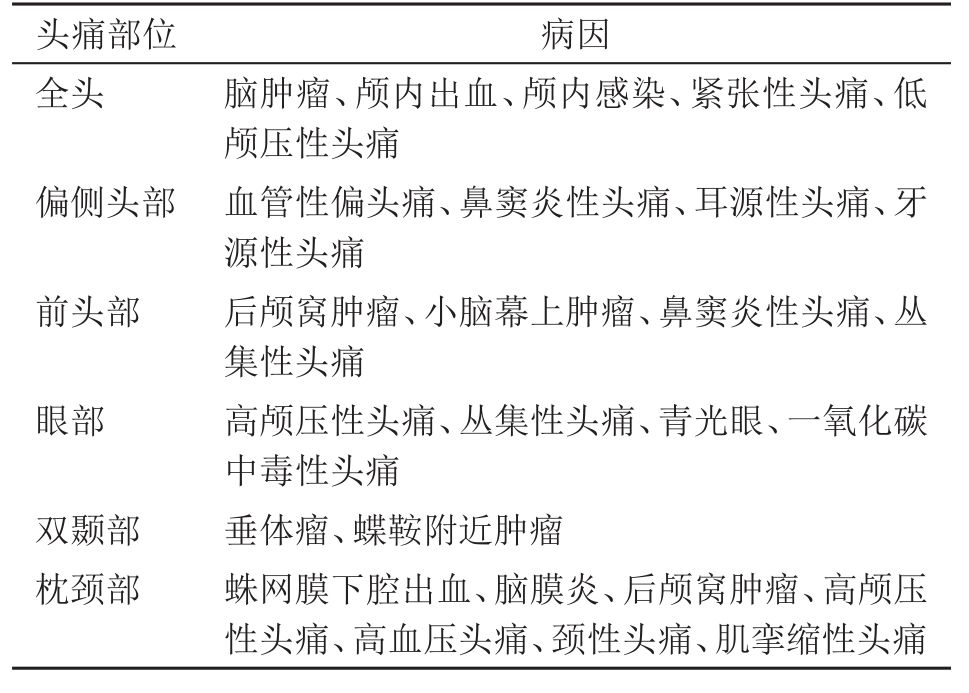
\includegraphics[width=3.21875in,height=2.30208in]{./images/Image00039.jpg}
\end{table}

\hypertarget{text00020.htmlux5cux23CHP1-7-2-1-1-4}{}
(4) 头痛的性质:

对头痛性质的了解十分重要。搏动性跳痛常为血管性头痛;发作性电击样剧痛为三叉神经痛的特征;咽后部发作性疼痛,可因吞咽动作诱发或加重者应考虑舌咽神经痛;紧箍样头痛多为肌紧张性头痛;眼、耳、鼻疾病所伴发者,大多数是胀痛或钝痛;神经症则是隐隐作痛,时轻时重。

\hypertarget{text00020.htmlux5cux23CHP1-7-2-1-1-5}{}
(5) 头痛的程度:

头痛的程度常不能反映病情的严重度,有时颅内占位性病变头痛并不严重而慢性焦虑症的头痛却表现剧烈难忍。一般而言,剧烈头痛常见于神经痛、偏头痛、蛛网膜下腔出血、脑膜炎等;中等度头痛,主要见于颅内占位性病变、慢性炎症等;轻度头痛,可见于神经症及某些邻近器官(耳、眼、鼻)病变。

\hypertarget{text00020.htmlux5cux23CHP1-7-2-1-1-6}{}
(6) 头痛发生的速度及影响因素:

急性突发性头痛,除多为血管性头痛外,尚有急性脑卒中(蛛网膜下腔出血、脑出血等)、急性感染性疾患。缓慢发生的头痛且进行性加重,并有颅内压增高表现者可能为颅内占位性病变,而无颅内压增高者可见于紧张性头痛。咳嗽、用力或头部转动,常使颅内压增高而头痛加剧;直立位可使肌紧张性头痛或腰穿后反应等加重,而丛集性头痛则减轻;压迫颞、额部动脉或颈总动脉可使血管性头痛减轻。根据头痛的发病方式和经过,对头痛进行鉴别诊断,见表\ref{tab7-2}。

\hypertarget{text00020.htmlux5cux23CHP1-7-2-1-1-7}{}
(7) 头痛的伴随症状:

头痛时常伴恶心、呕吐、面色苍白、出汗、心悸等自主神经症状,主要见于偏头痛;头痛严重并有进行性加剧的恶心、呕吐,常为颅内高压的征兆;体位变化时出现头痛加重或意识障碍,见于脑室内肿瘤、后颅凹或高颈段病变;伴有视力障碍及其他眼部征象(复视),呈短暂性发作者,多为偏头痛、椎-基底动脉供血不足;眼底视乳头水肿或出血,常为颅内压增高症或高血压性脑病。头痛伴精神症状(如淡漠或欣快)者应考虑额叶肿瘤的可能。由颅内损害引起的头痛常伴有神经功能缺失症状。

\hypertarget{text00020.htmlux5cux23CHP1-7-2-1-1-8}{}
(8) 其他病史:

尚需注意全身其他系统器官受损的病史,以及家族史、用药史、外伤史、手术史、月经及烟酒嗜好等。

\begin{table}[htbp]
\centering
\caption{头痛的发病方式和经过}
\label{tab7-2}
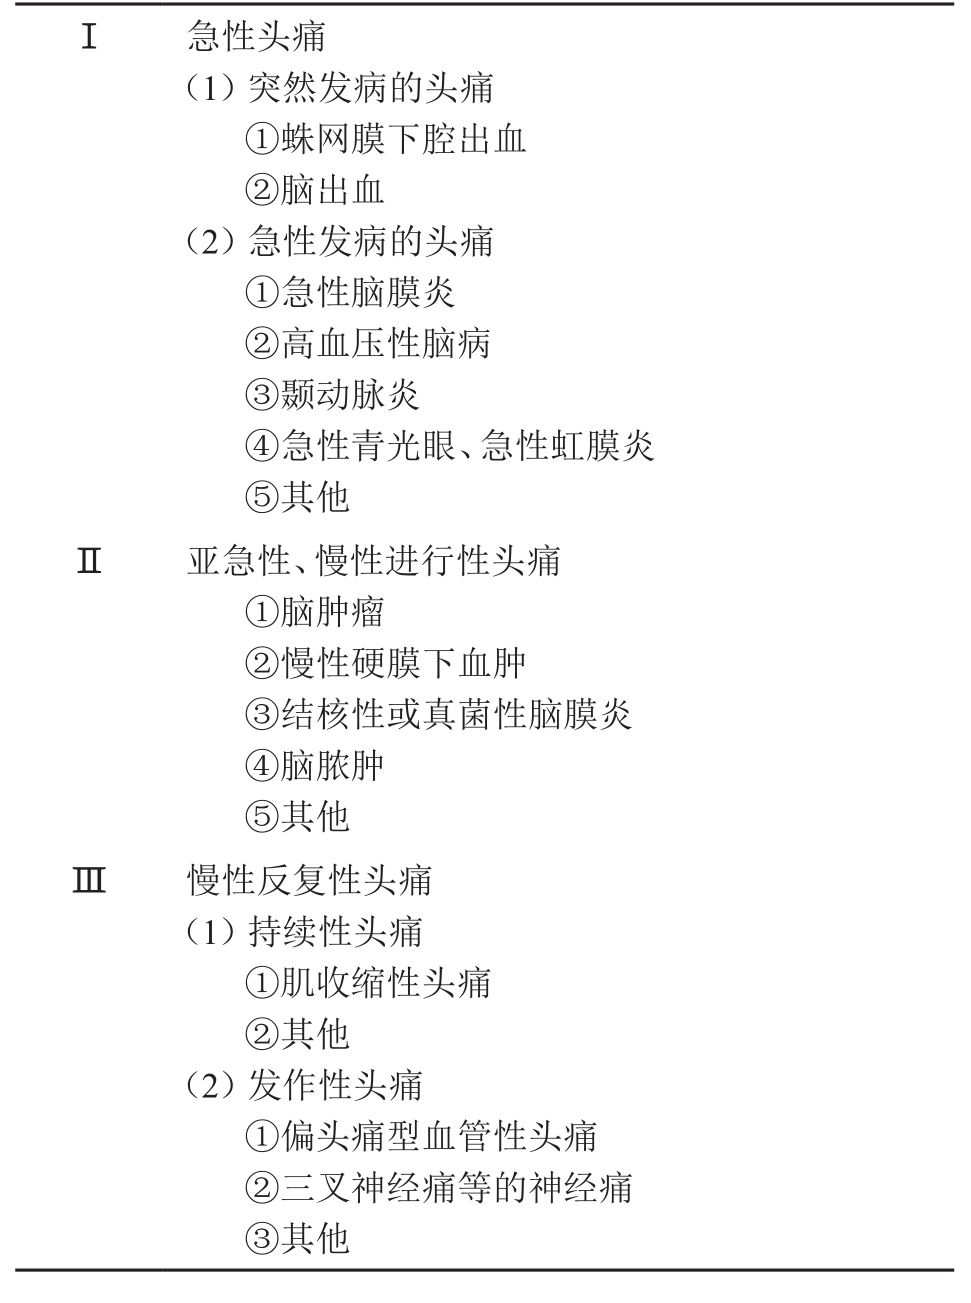
\includegraphics[width=3.22917in,height=4.33333in]{./images/Image00040.jpg}
\end{table}

\paragraph{体检}

全面详尽的体格检查尤其是神经系统和头颅五官的检查,有助于发现头痛的病变所在。

\hypertarget{text00020.htmlux5cux23CHP1-7-2-1-2-1}{}
(1) 内科检查:

许多内脏器官或系统的疾患可发生头痛,应按系统详细检查,大多可查出头痛的原因。如高血压、全身感染性疾病的发热或中暑、缺氧(如一氧化碳中毒),慢性肺部疾患的高碳酸血症,严重贫血或红细胞增多症,均可由于脑血流增加而致头痛;而毒素作用、酗酒,则可因血管扩张而致头痛。尚有代谢内分泌疾病的检查(甲亢、低血糖、嗜铬细胞瘤等)。

\hypertarget{text00020.htmlux5cux23CHP1-7-2-1-2-2}{}
(2) 五官检查:

头部邻近器官的疾病也是头痛常见的原因。如在眼部的视神经炎、儿童的屈光不正、青光眼、眼部表浅炎症(结膜炎、角膜炎、睑板腺炎、泪囊炎等)及眶部组织的炎症;在耳鼻咽喉方面有鼻炎、鼻窦炎、咽炎、中耳炎、鼻窦或鼻咽部肿瘤,另外颞颌关节病及严重的牙病也可引起头痛。

\hypertarget{text00020.htmlux5cux23CHP1-7-2-1-2-3}{}
(3) 神经系统检查:

全面的神经系统检查是非常重要的。

\hypertarget{text00020.htmlux5cux23CHP1-7-2-1-2-4}{}
(4) 精神检查:

有不少精神科疾病可伴有头痛,神经症是最常见的,而抑郁症的精神症状可被躯体症状所掩盖,尤其是隐匿性抑郁,常呈一些不典型的疼痛。

\paragraph{辅助检查}

应根据患者的具体情况和客观条件来选择性地应用。如做头颅X线检查、脑电图、CT扫描或MRI、腰穿脑脊液检查等,以及内科与五官科方面的检查。

头痛的临床检查方法见表\ref{tab7-3}。

\hypertarget{text00020.htmlux5cux23CHP1-7-2-2}{}
(二) 局限性病变抑或全身性病变

\paragraph{局限性病变}

包括颈部以上的局部病变引起的头痛,又可分为两大组:

\begin{table}[htbp]
\centering
\caption{头痛的临床检查方法}
\label{tab7-3}
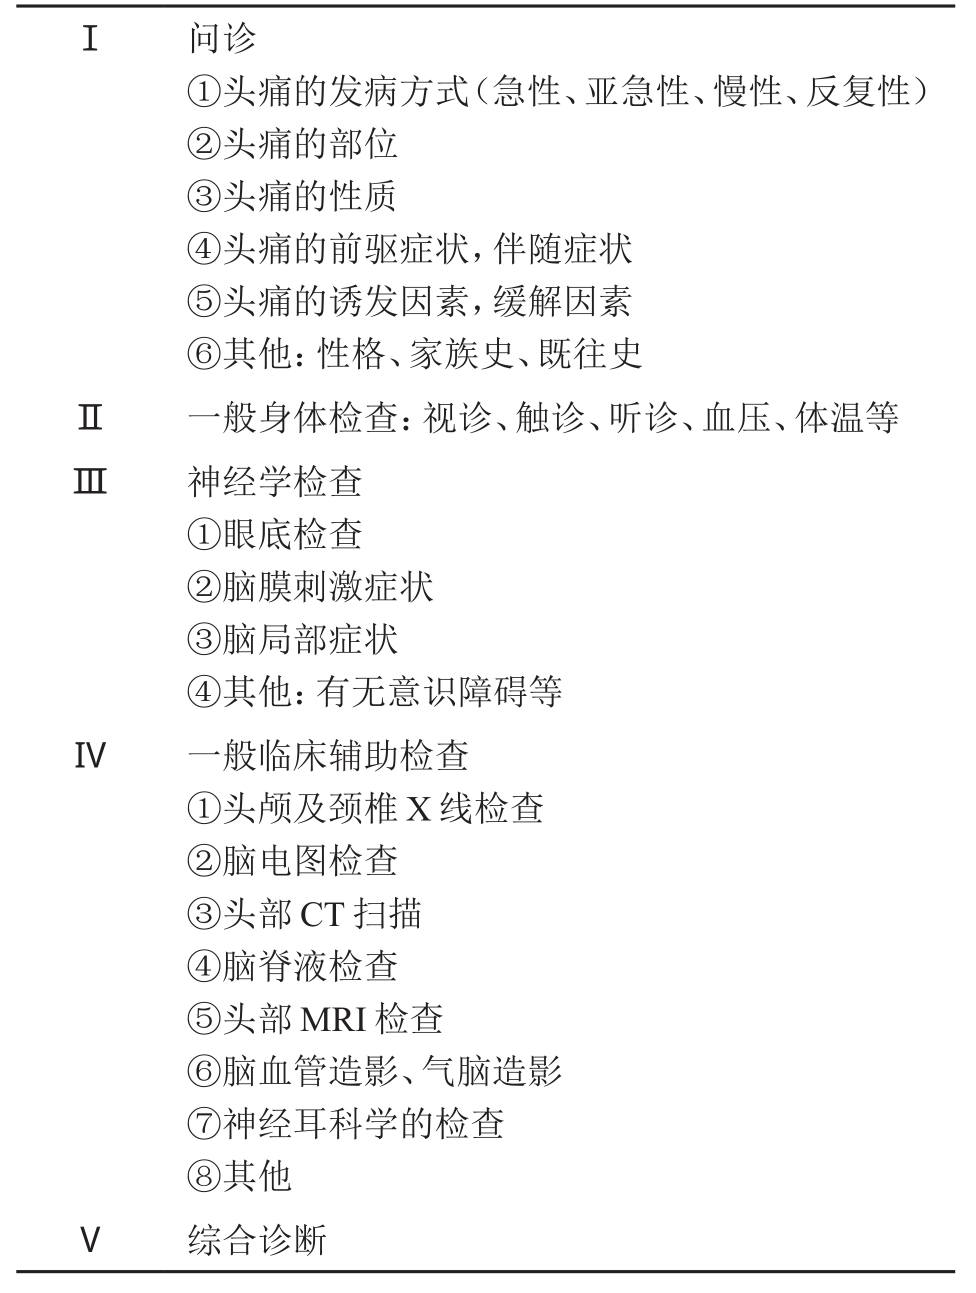
\includegraphics[width=3.25in,height=4.30208in]{./images/Image00041.jpg}
\end{table}

\hypertarget{text00020.htmlux5cux23CHP1-7-2-2-1-1}{}
(1) 颅内疾病:

此组疾病所致的头痛大都较严重,起病急,发展迅速。多数伴有恶心和(或)呕吐;部分尚有意识障碍或脑部和脑神经损害的表现,如抽搐、肢体瘫痪和瞳孔改变等。

\hypertarget{text00020.htmlux5cux23CHP1-7-2-2-1-2}{}
(2) 头颈部疾病:

此组疾病引起的头痛可轻可重,但很少逐渐加重。头痛的部位常与病灶一致或位于病灶附近,刺激病变部位可使疼痛加剧(如三叉神经痛等);但血管性头痛,压迫颞动脉则可使头痛减轻。头颈部疾病所致头痛的原发病灶明显,诊断不难。

\paragraph{全身性病变}

\hypertarget{text00020.htmlux5cux23CHP1-7-2-2-2-1}{}
(1) 全身性器质性病变:

引起急性头痛主要包括两大类疾病:一类是急性中毒。金属及化学物质如铅、锰、苯、酒精、一氧化碳等中毒时均可引起头痛。常为头部弥漫性跳痛,转动头部,头痛部位和性质无改变为此类头痛的重要特点。另一类是全身感染。多为急性传染病,头痛多在疾病的初期发生,也可出现在传染病的极期;无脑膜刺激征及神经系统定位征,脑脊液压力有时可增高,但生化及外观检查无异常。

\hypertarget{text00020.htmlux5cux23CHP1-7-2-2-2-2}{}
(2) 功能性病变:

多见于神经症患者,除头痛外,常伴有神经症的其他症状,如失眠、记忆力减退、注意力不集中、头昏、烦躁等,常因精神刺激而加重。患者一般情况好,临床检查无器质性病变存在。部分患者的头痛是由于服药后所引起(医源性头痛),主要是血管扩张剂等。应注意,功能性头痛必须在排除可能的器质性病变后才能确立。

\subsection{处理原则}

头痛的防治原则包括病因治疗、对症治疗和预防性治疗。对于病因明确的病例应尽早去除病因,如颅内感染应抗感染治疗,颅内高压者宜脱水降颅压等。任何头痛在急性发作时均应尽可能寻找潜在的病因进行治疗;对于病因不能立即纠正的继发性头痛及各种原发性头痛急性发作,可给予止痛等对症治疗以终止或减轻头痛症状。对慢性头痛呈反复发作者应给予适当的预防性治疗,以防头痛频繁发作。

\subsection{常见头痛的诊断与处理}

\hypertarget{text00020.htmlux5cux23CHP1-7-4-1}{}
(一) 偏头痛

偏头痛(migraine)是一种常见的慢性神经血管性疾患,是临床常见的原发性头痛,其特征是发作性、多为偏侧、中重度、搏动样头痛,一般持续4~72小时,可伴有恶心、呕吐,光、声刺激或日常活动均可加重头痛,安静环境、休息可缓解头痛。多起病于儿童和青春期,中青年期达发病高峰,女性多见,约50\%患者有家族史。精神紧张、过度劳累、气候骤变、强光刺激、烈日照射、低血糖、应用扩血管药物或利血平、食用高酪胺食物(如巧克力、乳酪、柑橘)及酒精类饮料,均可诱发偏头痛发作。

\paragraph{临床表现特点}

偏头痛有多种类型,但以以下两型常见:

\hypertarget{text00020.htmlux5cux23CHP1-7-4-1-1-1}{}
(1) 无先兆偏头痛(普通型偏头痛):

是最常见的偏头痛类型,约占80\%。临床表现为反复发作的一侧或双侧额颞部搏动性疼痛,常伴有恶心、呕吐、畏光、畏声、出汗、全身不适与头皮触痛等症状。通常在发作开始时仅为轻~中度的钝痛或不适感,数分钟至数小时后达到严重的搏动性痛或跳痛。有时疼痛放射至上颈部及肩部。部分女性患者发作常与月经有关,通常为经期前2天到经期的第3天之间发病,若90\%的发作与月经周期密切相关称月经期偏头痛。出现上述发作至少5次,除外颅内外各种器质性疾病后方可作出诊断。

\hypertarget{text00020.htmlux5cux23CHP1-7-4-1-1-2}{}
(2) 有先兆偏头痛(典型偏头痛):

约占偏头痛患者的10\%。一般在青春期发病,多有家族史,头痛发作前数小时至数日可有倦怠、注意力不集中和打哈欠等前驱症状。在头痛之前或头痛发生时,常以可逆的局灶性神经系统症状为先兆,表现为视觉、感觉、言语和运动的缺损或刺激症状。最常见为视觉先兆,常为双眼同向症状(homonymous
visual
symptoms),如视物模糊、暗点、闪光、亮点亮线或视物变形;其次为感觉先兆,感觉症状多呈面-手区域分布;言语和运动先兆少见。先兆症状一般在5~20分钟内逐渐形成,持续不超过60分钟;不同先兆可以接连出现。头痛在先兆同时或先兆后60分钟内发生,表现为一侧或双侧额颞部或眶后搏动性头痛,常伴有恶心、呕吐、畏光或畏声、苍白或出汗、多尿、易激怒、气味恐怖或疲劳感等,可见头面部水肿、颞动脉突出等。活动能使头痛加重,睡眠后可缓解头痛。头痛可持续4~72小时,消退后常有疲劳、倦怠、烦躁、无力和食欲差等,1~2日后常可好转。

有上述典型偏头痛症状,虽经治疗头痛时间持续在72小时以上(其间可能有短于4小时的缓解期)的称为偏头痛持续状态(status
migrainous)。

大多数偏头痛患者的预后良好,随年龄的增长症状可逐渐缓解,部分患者可在60~70岁时偏头痛不再发作。

\paragraph{治疗要点}

偏头痛的治疗目的为减轻或终止头痛发作,缓解伴发症状,预防头痛复发。

\hypertarget{text00020.htmlux5cux23CHP1-7-4-1-2-1}{}
(1) 发作期的治疗:

治疗药物包括非特异性止痛药如非甾体类抗炎药(NSAIDs)和阿片类药物,特异性药物如麦角类制剂(麦角胺1~2mg/次,日最大剂量6mg;双氢麦角胺肌肉注射1~2mg/次,日最大剂量4mg,或口服1~3mg/次,日最大剂量9mg)和曲普坦类药物,后者包括舒马曲普坦(皮下注射:6mg/次,日最大剂量12mg;口服25~100mg/次,日最大剂量300mg)、那拉曲普坦(口服2.5mg/次,日最大剂量5mg)、利扎曲普坦(口服5~10mg/次,日最大剂量30mg)、佐米曲普坦(口服2.5~5mg/次,日最大剂量10mg)和阿莫曲普坦(口服6.25~12.5mg/次,日最大剂量25mg)等。通常应在症状起始时立即服药。药物选择应根据头痛程度、伴随症状、既往用药情况等综合考虑,可采用阶梯法、分层选药,进行个体化治疗。①轻~中度头痛:单用NSAIDs如对乙酰氨基酚(口服0.3~0.6g/次,日最大剂量不超过2.0g)、萘普生(口服0.2~0.3g/次,每日2~3次)、布洛芬(口服0.2~0.4g/次,每日3~4次)等可有效,如无效再用偏头痛特异性治疗药物。阿片类制剂如哌替啶等,因有成瘾性,不推荐常规用于偏头痛的治疗,但对于有麦角类制剂或曲普坦类应用禁忌的病例,如合并心脏病、周围血管病或妊娠期偏头痛,则可给予哌替啶治疗以终止偏头痛急性发作。②中~重度头痛:可直接选用偏头痛特异性治疗药物以尽快改善症状,部分患者虽有严重头痛但以往发作对NSAIDs反应良好者,仍可选用NSAIDs。麦角类和曲普坦类药物不良反应包括恶心、呕吐、心悸、烦躁、焦虑、周围血管收缩,大量长期应用可引起高血压和肢体缺血性坏死。严重高血压、心脏病和孕妇患者均为禁忌。此外,应用过频,则会引起药物过量使用性头痛(medication-overuse
headache),因此,麦角类和曲普坦类药物每周用药不超过2~3天。③伴随症状:恶心呕吐可肌肉注射甲氧氯普胺10mg,严重呕吐者可用小剂量奋乃静、氯丙嗪。烦躁者可用地西泮10~20mg肌肉注射以促使患者镇静和入睡。

\hypertarget{text00020.htmlux5cux23CHP1-7-4-1-2-2}{}
(2) 预防性治疗:

适用于:①频繁发作,尤其是每周发作1次以上严重影响日常生活和工作的患者;②急性期治疗无效,或因副作用和禁忌证无法进行急性期治疗者;③可能导致永久性神经功能缺损的特殊变异型偏头痛,如偏瘫性偏头痛、基底型偏头痛或偏头痛性梗死等。常用药物有:①β受体阻滞剂:普萘洛尔(10~60mg/次,每天2次),美托洛尔(100~200mg/次,每天1次);②钙通道阻滞剂:氟桂利嗪(5~10mg,每日1次,睡前服用),维拉帕米(160~320mg/d);③抗癫痫药:丙戊酸钠(0.4~0.6g/次,每天2次),托吡酯(25~200mg/d),加巴喷丁(0.9~1.8g/d);④抗抑郁药:阿米替林(25~75mg睡前服用),丙米嗪和氟西汀等;⑤5-HT受体拮抗剂:苯噻啶(0.5~3mg/d)等。其中,普萘洛尔、阿米替林和丙戊酸钠三种在结构上无关的药物,是预防性治疗的支柱,一种药物无效可选用另一种药物。

\hypertarget{text00020.htmlux5cux23CHP1-7-4-2}{}
(二) 丛集性头痛

丛集性头痛(cluster
headache)是一种原发性神经血管性头痛。以男性多见,约为女性的3~4倍。头痛突然发生,无先兆症状,几乎于每日同一时间,常在晚上发作,使患者从睡眠中痛醒。头痛位于一侧眶周、眶上、眼球后和(或)颞部,呈尖锐、爆炸样、非搏动性剧痛。头痛达高峰时,患者常以手击头部、甚至以头撞墙,在室内外来回走动、十分烦躁、痛苦与不安。头痛持续15分钟~3小时不等。发作频度不一,从一日8次至隔日1次。疼痛时常伴有同侧颜面部自主神经功能症状,表现为结膜充血、流泪、流涕等副交感神经亢进症状,或瞳孔缩小和眼睑下垂等Horner征,较少伴有恶心、呕吐。头痛发作可连续数周至数月(常为2周~3个月),在此期间患者头痛呈一次接一次地成串发作,故名丛集性头痛。丛集发作期常在每年的春季和(或)秋季;丛集发作期后可有数月或数年的间歇期。在丛集期,饮酒或血管扩张药可诱发头痛发作,而在间歇期,两者均不会引起头痛发作。

根据中青年男性出现发作性单侧眶周、眶上和(或)颞部严重或极度严重的疼痛,可伴有同侧结膜充血、流泪、流涕、眼睑水肿、前额和面部出汗、瞳孔缩小、眼睑下垂等自主神经症状,发作时坐立不安、易激惹,并具有反复密集发作的特点,神经影像学排除引起头痛的颅内器质性疾患,可作出丛集性头痛的诊断。

本病急性期治疗方法有:①吸氧疗法:为头痛发作时首选的治疗措施。在发作剧烈时吸入纯氧(100\%氧气8~10L/min,10~20分钟)约使70\%患者终止发作。②利多卡因:用4\%~10\%利多卡因1ml经患侧鼻孔滴入,可使1/3的患者头痛缓解,机制是麻醉蝶腭神经节。③舒马曲普坦6mg皮下注射,或双氢麦角胺1~2mg肌肉注射等,可迅速缓解头痛。

本病预防性治疗药物包括维拉帕米、锂制剂和糖皮质激素等。维拉帕米240~320mg/d可有效预防本病发作,可在用药2~3周内发挥最大疗效。锂制剂适用于其他药物无效或有禁忌证者。糖皮质激素如泼尼松40~60mg/d,常可预防头痛的发作,第2周逐渐减量停药。其他药物有托吡酯、丙戊酸钠、苯噻啶、吲哚美辛等。

\hypertarget{text00020.htmlux5cux23CHP1-7-4-3}{}
(三) 紧张型头痛

紧张型头痛(tension-type headache)又称肌收缩性头痛(muscle contraction
headache),是双侧枕部或全头部紧缩性或压迫性头痛,约占头痛患者的40\%,是临床最常见的慢性头痛。主要由精神紧张及颅周肌肉张力增高引起。长期焦虑、紧张、抑郁或睡眠障碍,高强度的工作缺乏适当的放松及休息,以及某些单调工种使头、颈或肩胛带长期处于不良的姿势等均可为发病因素。头痛部位不定,可为双侧、单侧、全头部、颈项部、双侧枕部、双侧颞部等不同部位。通常呈持续性钝痛,像一条带子紧束头部或呈头周紧箍感、压迫感或沉重感。许多患者可伴有头昏、失眠、焦虑或抑郁等症状。有的患者也可出现恶心、畏光或畏声等症状。体检可发现疼痛部位肌肉触痛或压痛点,有时牵拉头发也有疼痛,颈肩部肌肉有僵硬感,捏压时肌肉感觉舒适。

根据患者的临床表现,排除颅颈部疾病如颈椎病、占位性病变和炎症性疾病等,通常可以确诊。

本病的许多治疗药物与偏头痛用药相同。对于焦虑、紧张或抑郁的患者应在精神上给予诱导和安慰,使其消除顾虑。对局限性的肌肉疼痛,如颈项肌和肩胛肌等可作按摩、针灸、理疗、局部封闭等治疗。急性发作期用对乙酰氨基酚、阿司匹林、非甾体抗炎药、麦角胺或双氢麦角胺等亦有效。对于频发性和慢性紧张型头痛,应采用预防性治疗,可选用阿米替林、丙米嗪或选择性5-羟色胺重摄取抑制剂(如舍曲林或氟西汀),或肌肉松弛剂如盐酸乙哌立松、巴氯芬等。失眠者可给予苯二氮{}
类如地西泮10~20mg/d口服。

\hypertarget{text00020.htmlux5cux23CHP1-7-4-4}{}
(四) 颅内压变化引起的头痛

\paragraph{颅内压增高所致的头痛}

脑瘤、硬膜下血肿、脑脓肿及其他占位性病变引起的头痛,在初期主要是因病变邻近疼痛敏感结构被牵拉、移位或因感觉神经直接受压所致。在后期是由于脑脊液循环通路被阻塞,导致颅内压增高,使远离病灶的对疼痛敏感结构被牵拉、扭曲和移位而引起头痛。初期的头痛常位于占位病变的同侧,在后期有颅内压增高时呈现为弥漫深在的持久性钝痛,晨起较重,在咳嗽、大便用力或打喷嚏时头痛加重。头痛程度一般不如偏头痛或颅内出血时那样严重,多数不影响睡眠。随着占位病变增大及颅内压增高,患者出现呕吐及视乳头水肿,最后因继发性视神经萎缩使视力减退或双目失明。治疗上除应用脱水剂降低颅内压外,根本措施是手术切除占位性病变。

良性颅内压增高征指有头痛和视乳头水肿等颅内压增高表现而无局灶性神经系统体征,抽搐、精神障碍,其脑室系统和脑脊液成分基本正常,颅内无占位性病变,预后较为良好的一种临床综合征。此症患者大都诉述有全面性的头痛,而并无脑部结构的移位,头痛可能是由于伴发的脑水肿牵引脑膜与脑血管的神经末梢所致。

\paragraph{低颅压性头痛}

低颅压性头痛(intracranial hypotension
headache)是脑脊液(CSF)压力降低(< 60mmH\textsubscript{2}
O)导致的头痛,多为体位性。患者常在直立后15分钟内出现头痛或头痛明显加剧,卧位后头痛缓解或消失。

低颅压性头痛包括自发性(特发性)和继发性两种。自发性病因不明,既往多认为可能与血管舒缩障碍引起CSF分泌减少或吸收增加有关;目前已证实多数自发性低颅压与自发性脑脊液漏有关。而导致自发性脑脊液漏可能与微小创伤和硬膜结构薄弱有关。部分病例有剧烈咳嗽、推举重物、剧烈体育活动等引起微小创伤的病史;部分病例可合并有结缔组织异常的其他疾病,如马方综合征(Marfan
syndrome)、常染色体显性遗传多囊肾、自发性视网膜脱离等。继发性可由多种原因引起,其中以硬膜或腰椎穿刺后低颅压性头痛最为多见,头颈部外伤及手术、脑室分流术、脊柱创伤或手术使CSF漏出增多,脱水、糖尿病酮症酸中毒、尿毒症、全身严重感染、脑膜脑炎、过度换气和低血压等使CSF生成减少。由于CSF量减少,压力降低,脑组织移位下沉等使颅内疼痛敏感组织被牵拉引起头痛。

本病可见于各种年龄,特发性多见于体弱女性,继发性无明显性别差异。头痛以双侧枕部或额部多见,也可为颞部或全头痛,但很少为单侧头痛,呈轻~中度钝痛或搏动性疼痛,缓慢加重,常伴恶心、呕吐、眩晕、耳鸣、颈僵和视物模糊等。头痛与体位有明显关系,立位时出现或加重,卧位时减轻或消失。脑组织下坠压迫脑神经也可引起视物模糊或视野缺损(视神经或视交叉受压)、面部麻木或疼痛(三叉神经受压)、面瘫或面肌痉挛(面神经受压)。

病因明确者应针对病因治疗,如控制感染、纠正脱水和糖尿病酮症酸中毒等。对手术或创伤后存在脑脊液瘘者可行瘘口修补术等。对症治疗包括头低位卧床休息,补液(2000~3000ml/d),穿紧身裤和束腹带,给予适量镇痛剂等。鞘内注射无菌生理盐水可使腰穿后头痛缓解。咖啡因可阻断腺苷受体,使颅内血管收缩,增加CSF压力和缓解头痛,可用苯甲酸钠咖啡因0.5g皮下或肌肉注射,或加入500~1000ml林格液中静脉滴注。硬膜外血贴疗法(epidural
blood
patching)是用自体血15~20ml缓慢注入腰或胸段硬膜外间隙,血液从注射点上下扩展数个椎间隙,可压迫硬膜囊和阻塞脑脊液漏出口,迅速缓解头痛,适用于腰穿后头痛和自发性低颅压性头痛,有效率97\%。腰穿时应选用口径细的穿刺针,术后去枕平卧至少6小时有利于预防头痛。

\hypertarget{text00020.htmlux5cux23CHP1-7-4-5}{}
(五) 脑血管病所致头痛

脑血管病所致头痛是急性头痛患者首先要甄别的,包括蛛网膜下腔出血、脑出血、缺血性卒中等。

\paragraph{蛛网膜下腔出血}

急性发作的头痛首先应考虑蛛网膜下腔出血的可能。典型症状为急性发作剧烈头痛,主诉为“刀劈样”、“爆炸样”头痛。70\%的头痛无定侧,可以为双额、顶、枕部或满头痛,30\%头痛偏向一侧,通常偏向动脉瘤所在侧。疼痛可放射至一侧或双侧眼部或颈部,可沿颈项向下放射,出现颈项强直,可持续数周至数月。可有意识丧失。也有一部分患者首发症状为精神错乱,惊厥发作,眩晕或脑神经(常为动眼神经瘫痪)障碍。腰穿脑脊液为均匀血性。患者如以往经常有阵发性头痛,此次头痛发作比较急剧,性质不同以往,也要考虑蛛网膜下腔出血。其处理参见第84章第4节“蛛网膜下腔出血”。

\paragraph{脑出血}

头痛常为首发症状,但往往迅速出现意识障碍与肢体偏瘫,结合血压突然升高的背景,诊断不难。

\paragraph{未破裂的脑动脉瘤与动静脉畸形}

一般在动脉瘤未破裂之前,头痛是不常见的。脑血管畸形头痛时常位于畸形同侧,如后交通动脉或颈内动脉瘤可以引起固定在同侧的眶、额部头痛。动脉瘤进一步扩张时可以出现眼肌瘫痪或对侧视野缺损,可以有局限性癫痫发作,对侧肢体偏瘫。DSA和(或)头颅MRI检查有助于诊断,治疗以手术为主。

\paragraph{缺血性脑卒中}

少数脑栓塞病例中有头痛症状,而在脑血栓形成中则头痛不常见。脑供血不足可致头痛,伴同感觉与运动障碍。头痛往往是搏动性的,可能是继发于颅外动脉的扩张。在椎-基底动脉或颈内动脉狭窄或闭塞的病例中,约1/3~1/2的患者有头痛,大都局限于枕部和颈部,或两额部;颈内动脉供血不足的头痛可以是同侧的或对侧的。

\paragraph{颞动脉炎}

颞动脉炎(temporal
arteritis)多见于中、老年人,头痛常位于头皮表浅部位以及颞部与眼眶周围部,也可较广泛地弥漫及额部与枕部,为一种强烈的搏动性和持续性疼痛,并且伴有在其他血管性头痛中所没有的烧灼感。平卧位或头低位头痛加剧,仰头或压迫颈总动脉时头痛减轻,咀嚼时头痛加重。咀嚼时出现头痛常为本病的首发症状。压迫眼球或眼球转动即出现眼窝部疼痛。头痛同时伴有面部肿胀、皮肤红肿、颞动脉明显扩张隆起呈蛇行状,搏动消失,触之有发硬肥厚感,压痛明显。部分病例视网膜动脉或脑动脉也可受累,可发生缺血性视神经炎而出现视力障碍。颞动脉炎多有发热、出汗、疲乏等全身症状,周围血象有白细胞增高,血沉增快。

本病如不加特殊治疗,通常在3~24个月内病情渐趋稳定或自愈,少数可持续几年。治疗主要用肾上腺皮质激素且疗效好,在激素开始治疗后数小时内体温即下降为正常,1~2天内局部疼痛和全身症状消失,食欲正常。头痛消失后激素可渐减量并维持用药数月,如停药后复发可重复再用。

\hypertarget{text00020.htmlux5cux23CHP1-7-4-6}{}
(六) 高血压性头痛

是一种非偏头痛型血管性头痛
。高血压病时约80\%出现不同程度头痛,且青壮年的高血压病头痛发生率高,其机制与动脉壁痛觉感受器受刺激有关。表现为头部沉重或间歇性钝痛、压迫感或搏动痛,或呈持续性全头或偏侧头痛,部位不固定,多在清晨或午前出现,在低头或屏气用力后头痛可加剧。恶性高血压伴高血压脑病或因嗜铬细胞瘤血压突然升高时均可出现剧烈的持续性头痛,常伴有恶心、呕吐、视力减退,视网膜出血或视乳头水肿。

高血压性头痛的治疗在于及时适度的降低血压。对伴有脑水肿者应及时应用脱水剂。

\hypertarget{text00020.htmlux5cux23CHP1-7-4-7}{}
(七) 颅脑外伤性头痛

急性和慢性头部外伤均可伴有头痛,常见的外伤后头痛有下列几种类型:①头皮裂伤或脑挫裂伤后瘢痕形成,刺激颅内外痛觉敏感结构而引起头痛。疼痛部位较局限,常伴局部皮肤痛觉过敏。②外伤后自主神经功能异常性头痛(dysautonomic
headache)是因颈前部受伤累及颈交感神经链,导致支配头颅的交感神经失去抑制而引起头痛。患者叙述一侧额颞区的发作性头痛,伴同侧瞳孔改变(先扩大后缩小),眼睑下垂及面部多汗。服用普萘洛尔(20mg,每天3次)对头痛有效。③外伤后因颈肌持续收缩而出现头痛,和紧张型头痛相似常有精神因素参与。④外伤后神经不稳定性头痛。常见于脑震荡后遗症,除头痛外尚有头晕、耳鸣、失眠、注意力不集中,记忆力衰退,精神萎靡不振或情绪易激动等症状。神经系统无器质性损害证据。

\hypertarget{text00020.htmlux5cux23CHP1-7-4-8}{}
(八) 五官疾病的头痛

眼源性头痛是指青光眼、虹膜炎、眼眶肿瘤、球后视神经炎、高度远视、眼外肌不平衡及用眼时间过长等原因引起球后或额颞区疼痛。急性乳突炎能引起耳后疼痛。病毒性膝状神经节带状疱疹所产生的疼痛常位于外耳道内或耳后,疼痛数日后出现带状疱疹及面瘫。鼻腔或鼻窦发炎时因黏膜充血水肿而引起鼻塞、流涕及牵涉性头痛。急性鼻窦炎时常引起眼球周围或额颞区头痛。因鼻窦内的脓性分泌物经过一夜睡眠后积聚增多,故患者清晨起床后头痛特别严重,待脓液排出后头痛明显减轻。X线检查有助于本病诊断。个别患者因鼻窦窦口被炎性分泌物或过敏性水肿阻塞,鼻窦内压力降低而形成“真空性头痛”(vacuum
headache)。牙病所致的头痛,多先有病牙部位疼痛,随后放射至同侧颞部,呈灼痛或跳痛,牙科检查可确诊。鼻腔肿瘤、颞下颌关节功能障碍(Costen综合征)及鼻咽癌均可引起头部牵涉痛。

\hypertarget{text00020.htmlux5cux23CHP1-7-4-9}{}
(九) 精神性头痛

神经症
、抑郁症等,经常出现头痛。其部位多不固定,多变,性质多样,呈钝痛、胀痛,易受外界或情绪影响,历时数周甚至数年。常伴睡眠及记忆、理解等精神方面的症状。

\hypertarget{text00020.htmlux5cux23CHP1-7-4-10}{}
(十) 神经痛

\paragraph{三叉神经痛(trigeminal neuralgia)}

是指三叉神经分布区内短暂的反复发作性剧痛。成年及老年人多见,40岁以上患者占70\%~80\%,女性多于男性。三叉神经痛可分为症状性和原发性,前者的病因为炎症(如疱疹病毒感染)、肿瘤(如半月神经节肿瘤)、动脉瘤及外伤等,后者系指病因未明者(可能因三叉神经脱髓鞘产生异位冲动或伪突触传递所致)。典型的原发性三叉神经痛通常有如下特点:①疼痛常局限于一侧,并以累及一支多见,少数患者可同时有二支或三支受累,且以上颌支(第2支)或下颌支(第3支)最常受累。②疼痛发作时表现为以面颊上下颌及舌部明显的剧烈电击样、刀割样、烧灼样或撕裂样疼痛,来去骤然,突发突止。疼痛由颌面或牙槽病灶开始,并沿该神经的支配区域放射,每次发作仅数秒钟至1~2分钟,间歇期正常,1天数次至1分钟多次。发作呈周期性,持续数周,可自行缓解数月或更长。随病程进展,缓解期日益缩短。③发作时可伴有同侧面部肌肉的反射性抽搐(故又称“痛性抽搐”),或有同侧面部潮红、流泪及流涎。④患者面部某个区域可能特别敏感,稍加触碰即引起疼痛发作,如上下唇、鼻翼外侧、舌侧缘、颊部等,该区域称之为“扳机点(触发点)”。发作期间面部的机械刺激,如说话、进食、洗脸、剃须、刷牙、打哈欠,甚至微风拂面皆可诱致疼痛发作,患者因而不敢大声说话、洗脸或进食,有的连口水也不敢咽下,严重影响患者生活,甚至全身营养状况不良,精神抑郁,有的产生消极情绪。

治疗主要有药物、封闭和手术治疗。药物治疗以卡马西平为首选,起始剂量0.1g口服,每天2~3次,最大剂量1.0g/d,有效维持量0.6~0.8g/d。如卡马西平无效可改用苯妥英钠0.1g口服,每天3次,如无效可每日增加0.05g,数日后加至0.6g/d。卡马西平或苯妥英钠单药治疗无效者两药合用可能有效。上述两药无效时可试用氯硝西泮(clonazepam)6~8mg/d口服。大剂量维生素B\textsubscript{12}
可缓解疼痛,剂量为1000~2000μg肌肉注射,每周2~3次,连用4~8周为一疗程。药物治疗无效者可试用无水乙醇或甘油封闭三叉神经分支或半月神经节,破坏感觉神经细胞,可获止痛效果,不良反应为注射区面部感觉缺失。经皮半月神经节射频电凝疗法也有较好疗效。三叉神经感觉根部分切除术,因止痛效果确切,仍是首选的手术治疗方法。而三叉神经显微血管减压术,止痛同时不产生感觉及运动障碍,是目前广泛应用的最安全有效的方法。

\paragraph{舌咽神经痛}

舌咽神经分布区的反复阵发性剧痛,不伴脑神经功能破坏表现的称舌咽神经痛(glossopharyngeal
neuralgia)。远比三叉神经痛少见。多数于中年起病,表现为口咽、喉或耳内的短暂发作性剧痛。每次持续数秒至1分钟,可因吞咽、咀嚼、讲话、咳嗽等触发。检查咽喉、舌根和扁桃体窝可有疼痛触发点。疼痛发作时可伴发咳嗽。个别患者发生昏厥,可能由于颈动脉窦神经过敏引起心脏停搏而造成。病程中可有自发缓解。神经系统检查无异常发现。将4\%可卡因或1\%丁卡因涂于患侧的口咽部,常可使疼痛缓解数小时。病因不明,有的可能是由于舌咽神经的脱髓鞘性病变引起,有的可能是由于局部的颅底血管压迫于舌咽神经所致。若疼痛持续,则本病需与鼻咽癌侵及颅底、耳咽管肿瘤、扁桃体肿瘤相鉴别。治疗与三叉神经痛相似。

\paragraph{枕神经痛}

枕神经痛(occipital
neuralgia)是枕大、枕小和耳大神经分布区疼痛的统称,三对神经来自C\textsubscript{2~3}
神经,分布于枕部。可因上段颈椎病、脊柱结核、骨关节炎、脊髓肿瘤、硬脊膜炎和转移瘤等所致,多为继发性神经损害;也可由上呼吸道感染或扁桃体炎引起,或病因不明。枕大神经分布于后枕部相当于两侧外耳道经头顶连线以后的部分;枕小神经主要分布于耳廓上部和枕外侧皮肤;耳大神经主要分布于耳廓下部前后面、腮腺表面和下颌角部皮肤。疼痛位于一侧枕部与颈部,呈阵发性刺痛或电击样痛,或持续性钝痛;患侧枕部头皮可有皮肤感觉过敏及局限性压痛点,可向头顶(枕大神经)、乳突部(枕小神经)或外耳(耳大神经)放射。枕大神经痛压痛点位于乳突与枕后粗隆间连线的中点;枕小神经痛的压痛点多位于该连线的外1/3处。部分患者在间歇期仍有钝痛。疼痛可为自发或因旋转尤其向对侧旋转而诱发,其他头颈部运动或咳嗽、喷嚏可使疼痛加重或诱发疼痛,故患者常不敢过分活动头部,或使头略向后仰并向患侧倾斜以缓解疼痛。除病因治疗外,可用止痛剂(卡马西平、苯妥英钠等)、神经营养剂(维生素B\textsubscript{1}
、B\textsubscript{12} 等)、局部封闭、理疗等对症治疗。


\hypertarget{text00021.htmlux5cux23CHP1-7-5}{}
参 考 文 献

1. 贾建平.神经病学.第6版,北京:人民卫生出版社,2008:158.

2. 头痛分类和诊断专家共识组
.头痛分类和诊断专家共识.中华神经科杂志,2007,40:439.

3. Schievink WI. Spontaneous spinal cerebrospinal fluid leaks and
intracranial hypotension. JAMA,2006,295:2286.

\protect\hypertarget{text00022.html}{}{}

\chapter{胸 痛}

胸痛是急诊室常见的患者就诊原因之一,临床上的胸痛不应仅是指解剖学胸部范围内的疼痛感受,而应包括任何原因所导致的解剖学胸部范围内的任何不适,同时也包括由于胸部疾患可能表现为其他部位的疼痛。由此可见导致胸痛的病因复杂,病情的严重程度相差很大。多数为良性经过的普通疾病,但其中有一部分则可能导致严重后果甚至危及生命。对于高危患者,症状发作后启动治疗越早,疗效越好,获益越多,任何延误都可能导致严重不良事件的发生,因此,急性胸痛患者的早期鉴别和危险分层对于识别高危患者并给予及时正确的处置具有重要意义。在临床急诊工作中,应首先确定就诊的急性胸痛患者是否患有急性心肌梗死、主动脉夹层、肺栓塞、气胸等,因为这些疾病若处理不及时,常危及生命。

\subsection{病因与发病机制}

\subsubsection{病因}

胸痛的主要病因大体上包括胸内结构病变、胸壁组织疾病、膈下脏器病变和功能性疾病等几个方面:

\paragraph{胸内结构病变}

\hypertarget{text00022.htmlux5cux23CHP1-8-1-1-1-1}{}
(1) 心源性胸痛:

心绞痛、急性心肌梗死、急性心包炎、主动脉夹层等。

\hypertarget{text00022.htmlux5cux23CHP1-8-1-1-1-2}{}
(2) 非心源性胸痛:

①大血管病变:主动脉瘤、肺梗死;②呼吸系统疾病:胸膜炎、自发性气胸等;③纵隔和膈肌的疾病:纵隔炎、纵隔脓肿、纵隔肿瘤和膈疝等;④食管疾病:反流性食管炎、食管破裂、食管裂孔疝等。

\paragraph{胸壁组织疾病}

带状疱疹、乳腺炎、皮下蜂窝组织炎、非化脓性肋软骨炎、肌炎、流行性肌炎、肋间神经炎、肋骨骨折等。

\paragraph{膈下脏器病变}

膈下脓肿、肝脓肿、脾梗死和肝癌破裂等。

\paragraph{功能性疾病}

心脏神经症。

\subsubsection{发病机制}

疼痛产生的机制:①各种化学或物理因素如缺氧、炎症、肌张力改变刺激肋间神经感觉纤维,脊髓后根传入纤维,支配气管、支气管及食管的迷走神经感觉纤维,膈神经的感觉纤维,支配心脏或主动脉感觉纤维等引起疼痛;②某一内脏与体表某一部位同受某些脊神经后根传入神经支配时,来自内脏的痛觉冲动传入大脑皮层区,除产生局部疼痛外,还可以出现相应体表的疼痛感觉------放射痛(又称牵涉痛)。

\subsection{诊断思路}

急性胸痛中包括了一组以胸痛为主要表现的疾病,其中危险性最高的分别是:急性心肌梗死、急性肺栓塞、主动脉夹层、张力性气胸及心包填塞。这些患者可能随时会发生死亡。急诊医生的任务是在众多表现为急性胸痛的患者中识别出这些高危的疾病并给予及时、适当的处理。这些高危的患者是否能够在急诊被及时准确地识别出来主要依靠:①急诊医生一定要时刻保持对这些疾病的警惕性;②急诊医生一定要掌握这些疾病主要的临床特征;③急诊科要有鉴别这些疾病的合理流程;④急诊科要能够提供必要的检查手段。

\subsubsection{临床特征}

首先在急诊处理急性胸痛的患者时,要利用有限的时间仔细询问病史和进行体格检查,这样能够确定下一步思考的正确方向。在询问病史时,要注意胸痛的部位、性质、缓解的因素,胸痛诱发和加重的因素,胸痛是否放射,胸痛的伴随症状和既往病史等。这些特征中往往隐含着具有诊断和鉴别诊断意义的线索,因此这些特征是医生接诊急性胸痛患者时需要重点询问的内容,相当部分的胸痛患者单纯依靠详细的病史询问就可以基本诊断。

\paragraph{发病年龄}

青壮年胸痛,应注意自发性气胸、心肌炎、心肌病、风湿性心瓣膜病,40岁以上患者应注意心绞痛、心肌梗死与肺癌。

\paragraph{胸痛部位}

包括疼痛部位及其放射部位。心绞痛与心肌梗死的疼痛常位于胸骨后或心前区,且放射到左肩和左上臂内侧。夹层动脉瘤疼痛位于胸背部,向下放射至下腹、腰部与两侧腹股沟和下肢。食管疾患、膈疝、纵隔肿瘤的疼痛也位于胸骨后。胸膜炎所致的胸痛常在胸廓的下侧部或前部。带状疱疹是成簇水疱沿一侧肋间神经分布伴剧痛,疱疹不越过体表中线。胸壁疾病特点为疼痛部位局限,局部有压痛。炎症性疾病,尚伴有局部红、肿、热表现。肝胆疾病或膈下脓肿可引起右下胸痛。

\paragraph{持续时间}

心绞痛发作时间短暂,持续数分钟,而心肌梗死疼痛持续时间很长且不易缓解。炎症、肿瘤、栓塞或梗死所致疼痛呈持续性。平滑肌痉挛或血管狭窄缺血所致疼痛为阵发性。

\paragraph{疼痛性质}

胸痛的程度可表现为剧烈的疼痛到轻微的隐痛,疼痛性质也多种多样。如带状疱疹呈刀割样痛或灼痛,剧烈难忍;肌痛呈酸痛;骨痛呈酸痛或锥痛。心绞痛常呈压榨样痛并伴有压迫感或窒息感;主动脉夹层动脉瘤常有突然出现的剧烈的撕裂痛。膈疝呈灼痛或膨胀感。早期肺癌可仅有胸部的钝痛或隐痛。食管疾病多表现为持续性隐痛或烧灼痛。

\paragraph{伴随症状}

气管、支气管疾病所致胸痛常伴有咳嗽、咳痰;食管疾病所致胸痛常伴有吞咽困难或咽下疼痛;肺梗死、原发性肺癌的胸痛常伴有小量咯血或痰中带血。

\paragraph{影响疼痛因素}

包括发生诱因、加重与缓解因素。胸膜炎、自发性气胸、心包炎所致胸痛常在深吸气及咳嗽时加重,停止呼吸运动则疼痛减轻或消失。劳累、体力活动、精神紧张,可诱发心绞痛发作,休息、含服硝酸酯类药物可使心绞痛缓解,而对心肌梗死疼痛则无效。反流性食管炎的胸骨后灼痛,饱餐后出现,仰卧或俯卧位加重,服用抗酸剂和促动力药后可减轻或消失。

\subsubsection{必要的体格检查}

对于急性胸痛患者,一般不可能进行全面、系统的体格检查,要求5分钟内完全必要的体格检查。因为大多数情况下病情不允许医生有充分的时间这样做,因此重要的是要有针对性,有目的地根据患者的病史特征和临床思维分析进行一些重点体查。

首先要注意生命征,包括血压、脉搏、呼吸、体温。发现患者血压<
90/60mmHg,心率> 100次/分钟,应立即启动稳定生命征治疗。

怀疑主动脉夹层对比双侧桡动脉、股动脉和足背动脉搏动,有怀疑应测四肢血压。

观察胸部表面皮肤有无局限性红肿、瘀斑和出血点及疱疹等;胸腹式呼吸协调性、呼吸形式和快慢深浅;双侧胸部对称性。胸膜炎、胸腹部外伤、膈下脓肿、单纯疱疹等疾病常有上述异常变化。触诊检查局部肿块、液波感、压痛和胸廓的呼吸动度。

注意胸壁感染、气胸、血胸、肋骨骨折等征象。女性乳腺炎也有以胸痛主诉就诊,注意鉴别。

听诊需了解双侧呼吸音对比、胸膜和心包摩擦音、肺干湿性啰音、哮鸣音、异常音和杂音等,这对鉴别心脏和肺部疾病有帮助。

怀疑肺栓塞的患者要注意检查下肢有无肿胀,是否有下肢深静脉血栓形成的证据。

\subsubsection{必要的辅助检查}

对胸痛的诊断,除需仔细了解病史、查体外,一些常规的辅助检查,如心电图(ECG)、心肌损伤标志物及影像学检查也十分重要,这对筛查潜在的高危胸痛患者有参考价值。

\paragraph{实验室检查}

血常规检查和凝血功能对判断有无感染和出凝血异常的存在必不可少。初始的ECG有助于确定中~高危的ACS患者,肌钙蛋白和心肌酶学是确诊是否存在心肌损害的重要手段,应用肌钙蛋白有助于确定是否需要早期血运重建,是ACS危险分层的重要工具;D-二聚体对急性肺栓塞的诊断有重要意义;动脉血气分析有助于了解肺功能情况。

\paragraph{心肌损伤标记物在胸痛患者中的应用价值}

心肌损伤标志物的测定能检出或除外心肌坏死,最常应用的生化标志物有肌钙蛋白T(TnT)和肌钙蛋白I(Tn
I)、肌红蛋白和肌酸激酶MB同工酶(CK-MB)。在急性胸痛的早期约3~6小时,肌红蛋白检测对除外心肌梗死的可能性很有价值,在症状发作7小时后,肌钙蛋白与CK-MB有较高的阴性预测性,Tn
I或TnT对诊断AMI的特异性与敏感性均较高。心肌损伤标记物浓度与心肌损害范围呈正相关。约30\%的非ST段升高的ACS患者cTn
I或cTnT升高,可能为非Q波心肌梗死而属高危患者,即使CK-MB正常,死亡危险性也增加。肌钙蛋白水平越高,危险性越高。

\paragraph{心电图}

ECG是胸痛患者应用广泛的检查方法。异常的心电图包括ST段升高、ST段下降和T波低平或倒置。入院时ECG有ST段升高的患者早期死亡率最高,ST段下降患者的死亡率中等,T波倒置最低。ST段升高是急性心肌梗死最敏感和最特异的ECG标志。新出现ST段升高的患者80\%~90\%为急性心肌梗死。约90\%的ECG有新出现的Q波为急性心肌梗死。ST段下降提示心肌缺血,但是其诊断进展性心肌梗死的可靠性差,仅约50\%的患者最终确诊为急性心肌梗死。对称性T波倒置的特异性较差,心肌缺血、心肌炎和肺栓塞在内的多种疾病都可以出现这种改变,约1/3的患者可能存在心肌梗死。有1/3左右的急性胸痛患者ECG正常,对这些患者动态观察心电图的变化很重要。在发病早期,很多急性心肌梗死最初的心电图无异常,随着时间的延长才表现为急性心肌梗死典型的ST段升高的ECG表现,若未对患者进行动态观察,常易忽略而漏诊。

目前建议在胸痛患者来诊10分钟内应进行ECG检查,10分钟内做出判定,ST段升高的患者一旦确定需立即进行再灌注治疗;ECG有缺血性表现的患者,按不稳定性心绞痛或非ST段升高的急性心肌梗死处理;ECG正常或有非特异性改变,应结合病史和生化标志物等综合判断。

\paragraph{影像学检查}

X线胸部透视与摄片,对于鉴别肺部疾病、肋骨、胸骨骨折,心脏各房室大小有帮助;CT扫描是一项对临床有较大帮助的检查,可以发现X线不能显示的病变,帮助临床诊断肺栓塞、主动脉瘤、夹层动脉瘤。心血管造影,尤其血管数字减影(DSA),可清楚显示主动脉瘤、主动脉夹层、室壁瘤的部位、大小、形态等情况;冠状动脉造影,可明确心肌梗死的部位和严重程度,是诊断心肌梗死的“金标准”;超声心动图实时显示心脏结构和动态以及心包积液。B超对膈下和肝脓肿、胆道情况以及包裹性胸水定位有意义。

\paragraph{放射性核素扫描}

对肺梗死、肺内占位病变、心肌梗死或局限性室壁瘤的诊断有帮助。

\paragraph{彩色多普勒超声}

对急性心肌梗死和急性大动脉夹层动脉瘤诊断的意义较大。彩超和多普勒可用于大动脉夹层的检查,但其具有一定的局限性。彩超仅能看到升主动脉和腹部、髂部的血管。主要的征象是主动脉明显增宽,主动脉壁分离形成的真腔与假腔,有时还可见内膜的裂口。超声还可用于鉴别胆石症、脾梗死、胰腺炎等一些膈下疾病。急性心肌梗死时二维超声心动图可见梗死的部位室壁运动低下、运动消失或反常运动。超声对急性肺栓塞的诊断帮助不大。超声对自发性气胸的诊断没有帮助。

\paragraph{胸痛患者辅助检查的顺序}

决定检查的顺序时要根据:危险性最大、最需要首先排除的疾病是什么?最能明确诊断的检查是什么?最方便、最及时的检查是什么?对于所有胸痛的患者,首先是要进行详细的体格检查,尤其是要注意生命体征,其次才是借助仪器的检查。有些疾病经过仔细的体格检查就能够发现特征性的表现,如剧烈胸痛者发现脉搏不对称及血管杂音强烈提示大动脉夹层等。切忌一切依赖仪器。对于一个急性胸痛的患者,辅助检查应该按照以下顺序进行为宜:

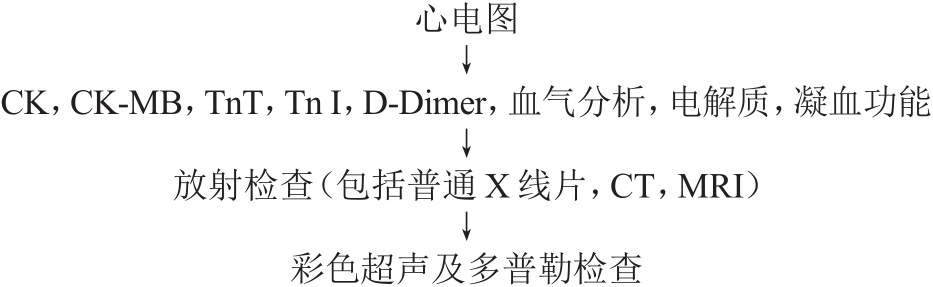
\includegraphics[width=3.09375in,height=0.94792in]{./images/Image00043.jpg}

\subsection{急诊处理原则和流程}

急性胸痛的急诊处理原则是:一是快速识别高危患者,以迅速进入快速救治绿色通道;剔除那些几乎没有或没有威胁生命疾病的患者;二是对不能明确诊断的患者应常规留院观察病情的演变,严防患者院外发生严重危及生命的事件。

1.首先判断病情严重性
,对生命征不稳定的患者,应立即开始稳定生命征的治疗;同时开始下一步处理;

2.对于生命征稳定的患者,首先获取病史和体征;

3.进行针对性的辅助检查;

4.在上述程序完成后能够明确病因的患者立即开始有针对性地病因治疗;

5.对不能明确病因的患者,建议留院观察,每隔30分钟复查一次心电图,每隔2小时复查心肌损伤标志物。心电图连续3次无变化,心肌损伤标志物连续2次无异常者在6~12小时后可予以出院。具体处理流程见图\ref{fig8-1}。

\begin{figure}[!htbp]
 \centering
 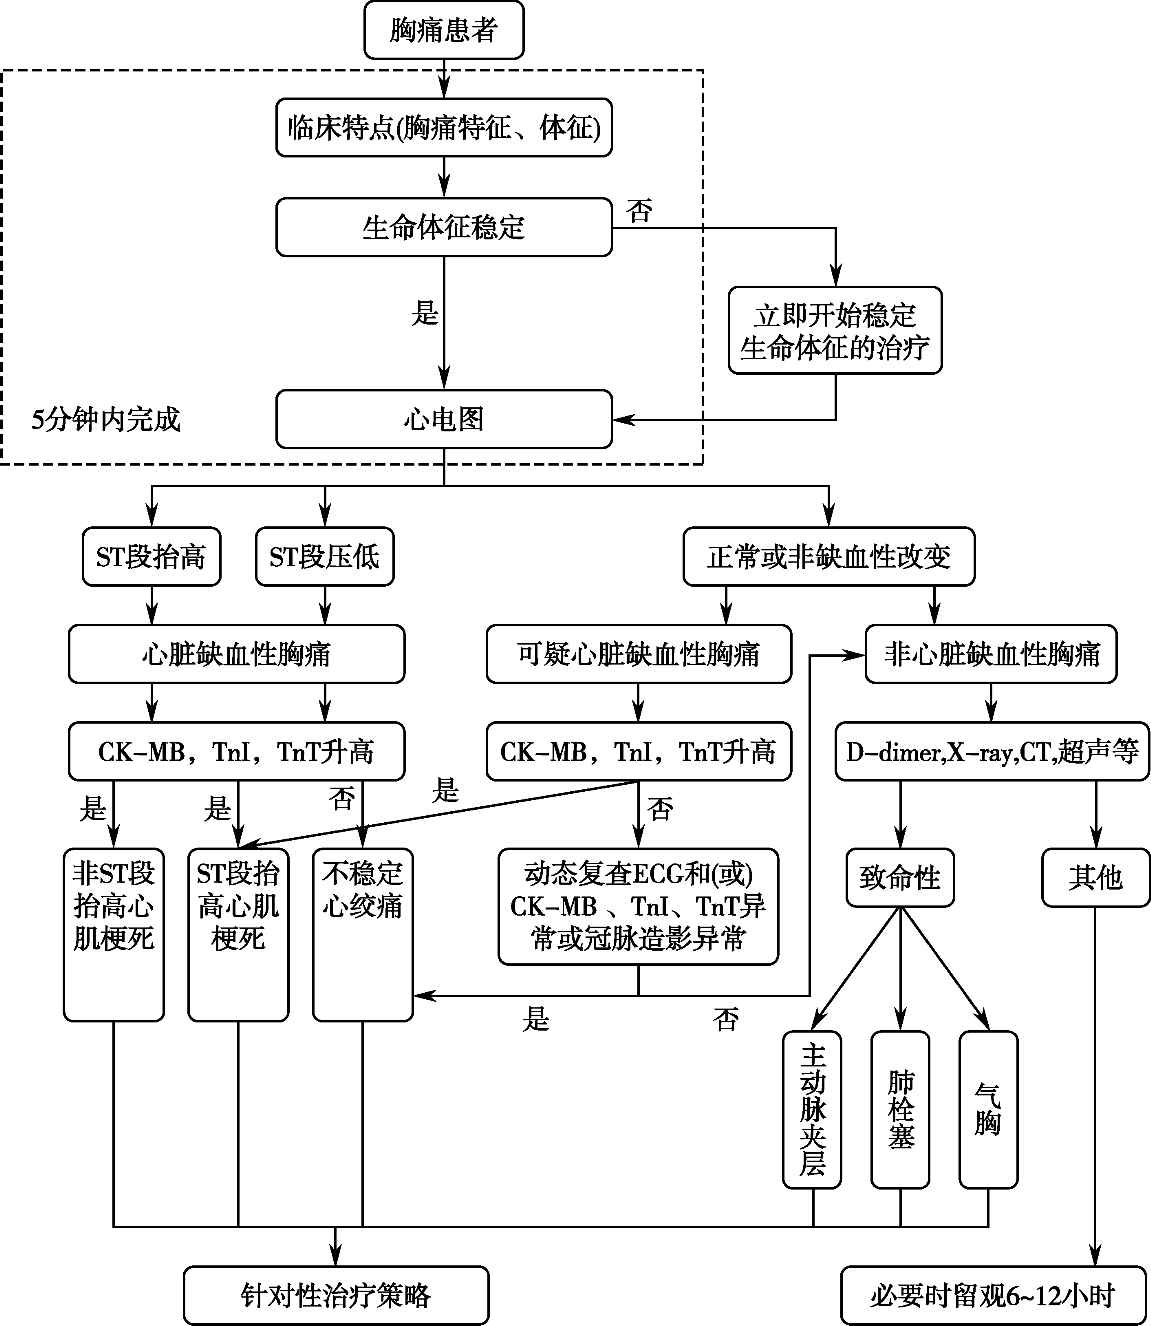
\includegraphics[width=4.69792in,height=5.41667in]{./images/Image00044.jpg}
 \captionsetup{justification=centering}
 \caption{胸痛的处理流程图}
 \label{fig8-1}
  \end{figure} 

\hypertarget{text00023.htmlux5cux23CHP1-8-4}{}
参 考 文 献

1. O'Connor R E,Bossaert L,Arntz H R,et al. Acute Coronary
Syndromes:2010 International Consensus on Cardiopulmonary Resuscitation
and Emergency Cardiovascular Care Science With Treatment
Recommendations. Circulation,2010,122: S422-S465.

2. Braunwald E,Antman E M,Beasley J W,et al. ACC/AHA Guideline Update
for the Management of Patients With Unstable Angina and Non-ST-Segment
Elevation Myocardial Infarction---2002:Summary Article:A Report of the
American College of Cardiology/American Heart Association Task Force on
Practice Guidelines(Committee on the Management of Patients With
Unstable Angina).Circulation,2002,106:1893-1900.

3. 罗学宏.急诊医学.北京:高等教育出版社,2008.74-78.

\protect\hypertarget{text00024.html}{}{}

\chapter{咯 血}

咯血(hemoptysis)是指喉腔、气管、支气管和肺组织出血,由咳嗽动作经口腔排出。咯血的临床过程难以预料,有时,初始仅少量痰中带血,却可以是大量的致命性咯血的先兆。大咯血引起失血性休克而致死的较少见,更常见的是大量的血淹溺肺泡,阻塞气道,因窒息和顽固性低氧血症而导致患者死亡。

咯血量可因病因和病变性质的不同而有差异,与病变的严重程度也不完全一致。临床上多根据咯血量将其分为少量咯血:24小时内咯血量≤100ml,包括痰中带血;中等量咯血:24小时内咯血量100~500ml;大咯血:24小时内咯血量>
500ml或一次咯血量≥200ml。大咯血约占全部咯血患者的1\%~4\%,但其死亡率高达80\%以上。

大咯血致死的危险与咯血量、出血速度、肺内潴留的血量以及患者基础肺功能储备相关,而与咯血的病因无关。年老体弱或久病无力者咳嗽乏力、基础肺功能差,即使几口血痰也可窒息致死。

\subsection{病因与发病机制}

\subsubsection{病因}

咯血的病因很多(表\ref{tab9-1}),但以肺结核、支气管扩张症、肺癌和肺炎等4种疾病多见。

尽管当今的检查手段有了长足的发展,对咯血患者采用了各种检查方法,但仍可有5\%~15\%的患者咯血原因不明,这类患者称隐匿性咯血(occult
hemoptysis)。部分隐匿性咯血可能由于气管、支气管的非特异性溃疡、静脉曲张、早期腺瘤、支气管小结石及轻微支气管扩张等病变引起。

\subsubsection{发病机制}

许多肺内外疾病和全身性疾病均可引起咯血,但咯血的机制有所不同。一般说来,炎症或肿瘤多导致病灶局部的毛细血管破坏,如不侵蚀支气管动脉,则咯血量一般较小。病变若侵蚀小动脉、小动静脉瘤或黏膜下静脉破裂则常常出现中等量或大咯血,而全身性疾病或严重而广泛的毛细血管炎症导致的咯血大多为中等量。小到中等量咯血大多可以自行终止,所以咯血很少引起失血性休克。

\begin{table}[htbp]
\centering
\caption{咯血的常见病因}
\label{tab9-1}
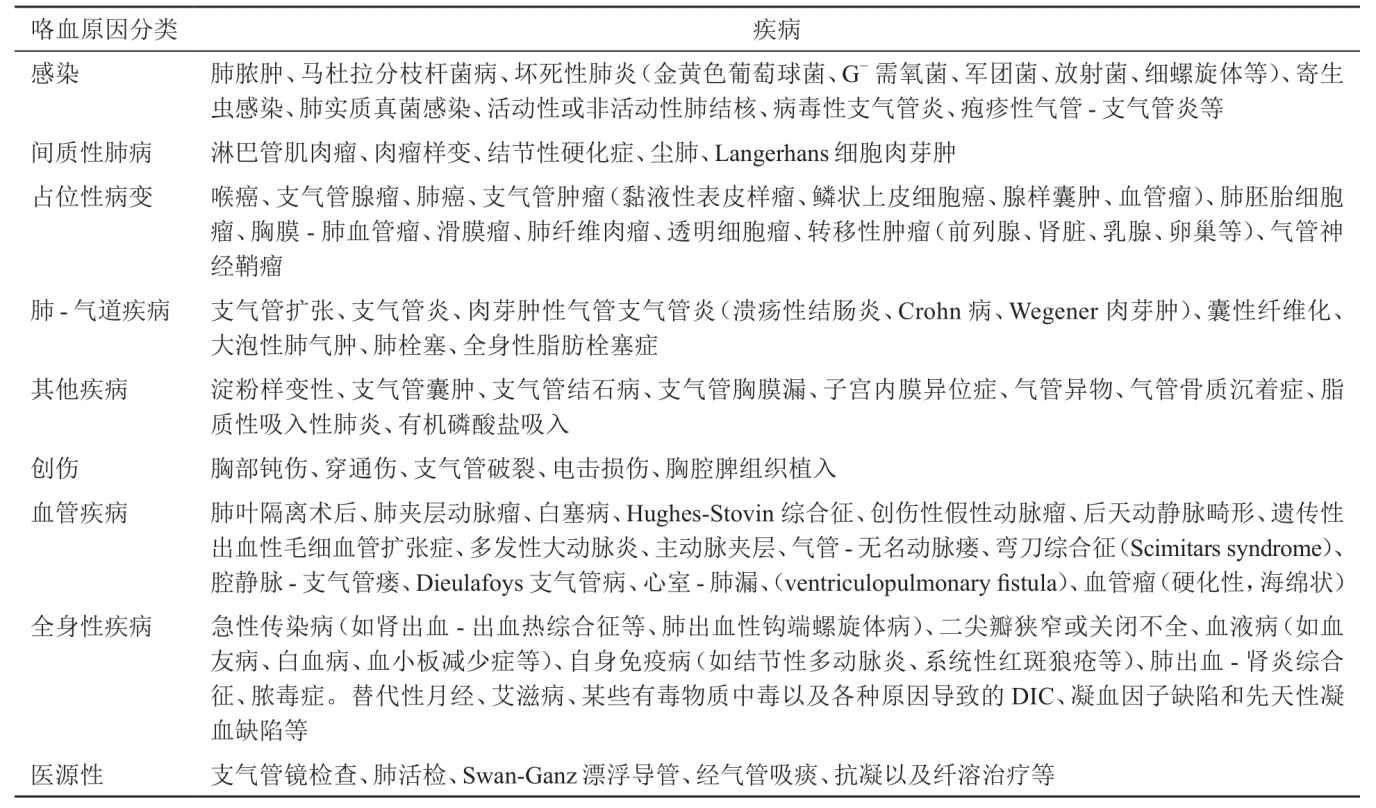
\includegraphics[width=6.59375in,height=3.875in]{./images/Image00045.jpg}
\end{table}

\paragraph{气管、支气管疾病}

各种病原微生物如细菌、病毒、支原体、寄生虫以及肿瘤、各种粉尘、异物、结石等,均可侵蚀气道邻近血管或肺泡毛细血管导致咯血。支气管扩张导致的咯血常见,炎性病变侵蚀血管壁,使血管弹性纤维遭到破坏或在支气管壁下形成假性动脉瘤,当用力咳嗽时血管破裂导致大咯血;癌组织可直接侵蚀血管壁破裂导致咯血,少到痰中带血,多到大咯血窒息均可发生。

\paragraph{肺部疾病}

许多肺部病变可直接侵蚀血管致使破裂出血或肺毛细血管床广泛损伤出血。大咯血最常见于肺结核(尤见于空洞性肺结核)、急性肺脓肿、癌性坏死及空洞形成、肺囊肿继发感染等,其穿行的支气管动脉或肺动脉受蚀,或动脉壁肌纤维破坏形成假性动脉瘤因咳嗽而破裂出血。此类咯血可因血凝块暂时充填空洞而压迫血管暂停出血,但也可因血凝块自溶而再次出现咯血。慢性肺脓肿多引起小量咯血,偶有大咯血发生。

\paragraph{肺血管病变或先天性病变}

支气管动脉-肺动脉瘘是由于肺动脉因体循环压力,形成动脉瘤,破溃出血。肺动脉栓塞、多动脉炎、白塞病的病变基础多为栓塞性动脉炎或动脉瘤样扩张。夹层动脉瘤或梅毒性动脉瘤,偶与支气管动脉相通,可造成致命性大咯血。原发性肺动脉高压可因肺动脉远端阻力加大,肺动脉与肺毛细血管形成侧支循环,当血管破裂时引起咯血。偶见于先天性肺动-静脉瘘,先天性毛细血管扩张症引起的咯血。

\paragraph{心血管疾病}

最常见的原因是二尖瓣狭窄和冠心病、心肌病等疾病导致的急性左心功能不全。左房血流受阻造成左房压力高,心脏前负荷增加,肺毛细血管及肺静脉压力升高,导致肺血管扩张,肺处于淤血状态,可引起肺水肿,并导致支气管黏膜下小静脉曲张,常自发或在炎症诱发下引起小静脉及毛细血管破裂,导致大咯血。

\paragraph{全身性疾病}

脓毒症、肾出血-出血热综合征、出血型钩端螺旋体病等急性全身感染性疾病、血液病和某些自身免疫性疾病如大动脉炎、白塞病、系统性红斑狼疮、肺出血-肾炎综合征(Goodpasture
syndrome)、子宫内膜异位症等病变,使肺微血管和毛细血管受损,血管内皮细胞功能障碍,血管脆性增加以及血小板减少或功能障碍导致出血。此类咯血多为弥漫性肺泡出血。

\paragraph{出凝血机制障碍}

包括血液系统疾病及DIC所致的咯血,多为全身多脏器出血的一部分。多见于全身性疾病导致的血小板减少和(或)功能障碍、凝血因子缺乏和(或)功能异常。此类咯血为原发病的继发性改变,罕见情况下咯血可能为首发症状。

\subsection{诊断思路}

多数咯血患者为突然起病,尤其第一次见到咯出鲜血,精神高度紧张,甚至有恐惧感,往往不能正确的诉说相关的症状及所见到血液的性状。因此,明确出血部位和出血原因显得尤为重要。

\paragraph{确定出血部位}

口腔、鼻腔、咽喉部以及消化道出血有时可误认为咯血,特别是后鼻道出血多流入口腔或食管出血未经胃酸作用直接呕出时,有时会出现刺激性咳嗽而导致对出血部位判断的错误,即所谓的“假性咯血”(pseudo-hemoptysis)。对首次从口腔内咳或呕血者,在不能判断出血部位的情况下,应仔细寻找出血部位。对可疑鼻咽部出血者,应迅速邀请专科会诊以明确诊断。详细询问病史和仔细的体格检查多能明确。呕血在大多数情况下诊断并无困难,在临床上可依据临床表现、体格检查、辅助检查和实验室检查予以区别。

\paragraph{临床表现特点}

除有原发病症状与体征外,大多数情况下,患者咯血前常有喉部痒感,血呈弱碱性,色鲜红,呈泡沫状,多混有痰液,咯血后数天内仍可咳出血痰。常见咯血病因的临床表现特点见表\ref{tab9-2}。

\begin{table}[htbp]
\centering
\caption{常见咯血原因的临床表现特点}
\label{tab9-2}
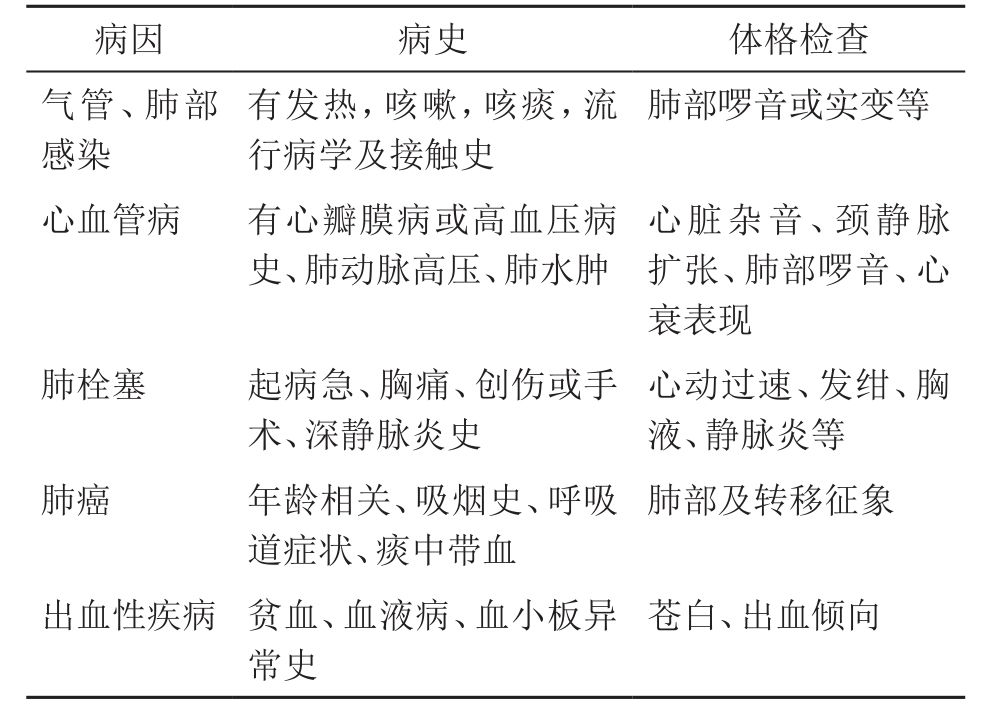
\includegraphics[width=3.26042in,height=2.38542in]{./images/Image00046.jpg}
\end{table}

大量咯血可引起急性出血性休克而出现面色苍白、冷汗、四肢湿凉,血管充盈度下降,血压降低等表现。因血凝块阻塞气道出现窒息的特征为咯血量突然减少或停止,同时出现胸闷、双手抓胸、喉头异常作响、继而烦躁不安、表情呆滞或恐惧、目瞪口张、全身发绀、呼吸变浅、速率加快,大小便失禁,肺部检查可见一侧或双侧呼吸音消失,进而呼吸突然停止。其他还包括肺不张和肺部继发感染等并发症的临床表现。

\paragraph{咯血与呕血的鉴别}

大量呕血时,鲜红色血液可从口腔及鼻腔涌出,或大咯血时部分血液咽下,复又呕出,致使咯血与呕血不宜鉴别。正确的鉴别诊断有助于采取恰当的治疗措施。咯血与呕血的鉴别见表\ref{tab9-3}。

\begin{table}[htbp]
\centering
\caption{咯血与呕血的鉴别}
\label{tab9-3}
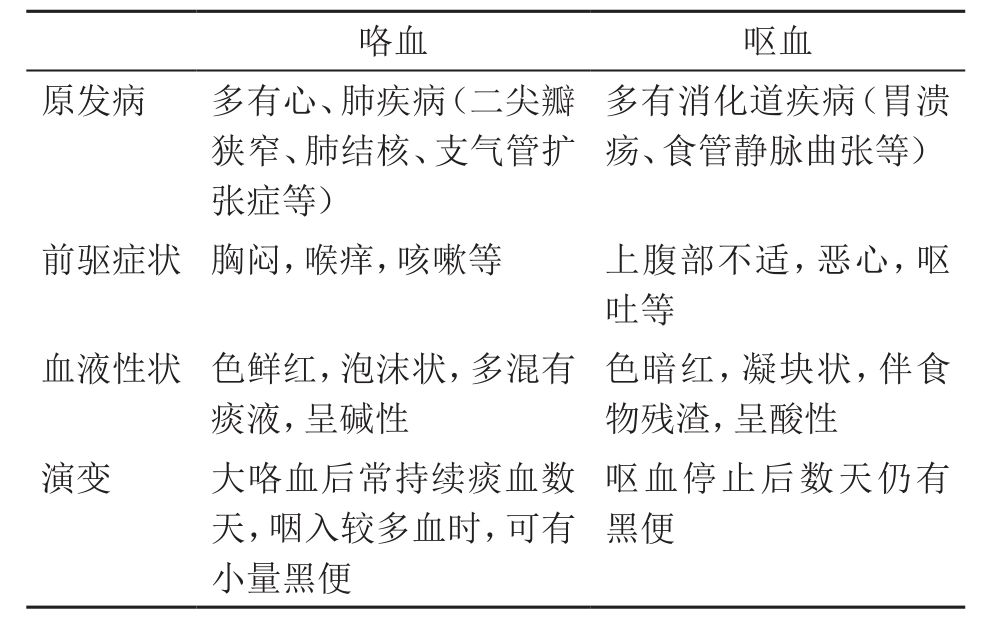
\includegraphics[width=3.26042in,height=2.05208in]{./images/Image00047.jpg}
\end{table}

\paragraph{辅助检查与实验室检查}

\hypertarget{text00024.htmlux5cux23CHP1-9-2-4-1}{}
(1) 影像学检查:

胸部X线可初步判断胸部病变的性质和部位。胸部CT检查有助于支气管、肺部和胸腔疾病的病因诊断。尤其是高分辨CT(HRCT)可显示次级肺小叶为基本单位的细微结构,可明确病变的性质及范围,基本上已代替支气管造影。HRCT及核素扫描可明确心肺血管病变及占位性病变。必要时可作支气管动脉造影,但一般仅用于介入治疗前对出血部位的精准定位。

\hypertarget{text00024.htmlux5cux23CHP1-9-2-4-2}{}
(2) 超声与心电图检查:

心脏彩色多普勒与心电图检查对心脏病变诊断有帮助,可发现各种类型心脏结构改变、心律失常、ST-T段等改变。腹部B超有助于了解肝、脾、腹水、腹腔肿物等情况。

\hypertarget{text00024.htmlux5cux23CHP1-9-2-4-3}{}
(3) 血常规及生化检查:

可见白细胞总数增加,以中性粒细胞增加为主时提示感染存在。出血较多时可见红细胞和血红蛋白含量下降,血小板可正常。凝血功能、肝功能、肾功能等异常均能对其原发病提供参考。血气分析有助于发现病情较重患者的低氧血症。

\hypertarget{text00024.htmlux5cux23CHP1-9-2-4-4}{}
(4) 痰液检查:

细菌、真菌和细胞学检查有助于原发病的诊断和治疗。

\hypertarget{text00024.htmlux5cux23CHP1-9-2-4-5}{}
(5) 特异性检查:

如结核菌素试验、免疫学检查有时会对结核病、结缔组织疾病的诊断具有重要参考价值。

\hypertarget{text00024.htmlux5cux23CHP1-9-2-4-6}{}
(6) 纤维支气管镜检查:

可发现部分患者的出血部位和性质,并可在镜下止血,同时还可进行局部灌洗、标本取样做病原学和细胞学检查。

\hypertarget{text00024.htmlux5cux23CHP1-9-2-4-7}{}
(7) 动脉造影:

支气管动脉造影可显示区域性支气管动脉异常,确定出血部位,是决定进行栓塞治疗的主要依据。肺动脉造影对来自肺动脉的大咯血,尤其是支气管动脉栓塞后继续出血者适用。对空洞性肺结核或其他肺化脓性疾病、疑Rasmussen动脉瘤或肺动静脉瘘所致的咯血,选择性支气管动脉及肺动脉造影应同时进行,若病变波及双重动脉系统,则可以同时作栓塞治疗,以免术后继续出血。

\paragraph{常见疾病鉴别诊断}

通过询问与咯血相关的病史、诱因、咯血量和伴随症状以及详细的体格检查多能寻找到原发疾病的线索。体格检查应注意有无肺部啰音、皮肤黏膜有无出血、淋巴结是否肿大、有无肝脾肿大、心脏杂音及体重减轻等。出血部位的判断可根据肺部体征及X线检查确定。

\hypertarget{text00024.htmlux5cux23CHP1-9-2-5-1}{}
(1) 支气管扩张:

缓慢起病,反复咳嗽伴脓痰和(或)量不等的咯血。既往多有麻疹、肺炎或免疫缺陷等病史。部分患者咯血为唯一症状,即所谓的“干性支气管扩张”。部分患者表现为反复发生的同一肺段感染,并迁延不愈,查体可闻及患侧固定而持久的湿啰音,可见杵状指(趾)等。胸部X线摄片或CT均可明确诊断。

\hypertarget{text00024.htmlux5cux23CHP1-9-2-5-2}{}
(2) 肺结核:

活动期多有午后低热、乏力、食欲减退、盗汗等结核中毒症状,部分可有不规则性高热。痰检或培养结核分枝杆菌阳性。查体可见结核面容、消瘦,局部湿啰音等。胸部X线摄片或CT表现多种形态,如局部渗出、增殖、纤维化、干酪性病变、钙化或空洞形成,以肺上叶尖后段及后基底段多见,可伴有胸腔积液、胸膜肥厚与粘连。聚合酶链反应(PCR)及结核菌素纯蛋白衍生物实验(purified
protein
derivative,PPD)有助于确定诊断,但后者不能区分是自然感染还是卡介苗免疫反应。

\hypertarget{text00024.htmlux5cux23CHP1-9-2-5-3}{}
(3) 肺癌:

持续出现咳嗽、咳痰,不明原因体重下降,近期痰中带血,反复出现。晚期可出现与呼吸运动有关联的胸痛及血性胸腔积液。查体可见气促、肺局限性喘鸣音、呼吸音增强或单侧胸腔积液、转移性骨压痛、淋巴结肿大(以颈部、腋窝为主,右锁骨上窝淋巴结肿大具有特殊诊断意义)等。胸部X线摄片或CT有助于诊断,痰液细胞学及活检可明确诊断。

\hypertarget{text00024.htmlux5cux23CHP1-9-2-5-4}{}
(4) 肺脓肿:

急性起病,多有劳累、受凉等病史。高热伴有不同程度的咯血。发病两周左右突然咳出大量脓痰及坏死组织,痰咳出后,体温下降。查体可发现局部湿啰音,偶可闻及空瓮音,宜可见杵状指(趾)。胸部X线摄片或CT和痰液细菌培养阳性多能明确诊断。

\hypertarget{text00024.htmlux5cux23CHP1-9-2-5-5}{}
(5) 风湿性二尖瓣狭窄:

有风湿性心脏病史。常在感冒、活动后出现呼吸困难,严重时不能平卧,常出现急性左心功能不全表现,伴以咳出大量粉红色泡沫样痰。小量咯血多见,偶见大量咯血。查体可见“二尖瓣面容”,心尖部听诊可及第一心音亢进、开瓣音、舒张中晚期隆隆样杂音、肺动脉瓣区第二心音亢进等,部分患者可摸到舒张期震颤。心脏多普勒超声检查可明确诊断。

\hypertarget{text00024.htmlux5cux23CHP1-9-2-5-6}{}
(6) 急性肺梗死:

有长期卧床、骨折、静脉炎或心房纤颤等病史。突然出现胸痛、胸闷、心悸、烦躁、冷汗,甚至晕厥,以小~中等量咯血多见。查体可见呼吸加快,肺局部叩诊浊音、呼吸音减弱及干湿性啰音。严重者可见急性右心衰表现,如心率加快、肺动脉瓣第二心音亢进、三尖瓣区可闻及收缩期杂音,可伴心律失常。血压下降,颈静脉怒张,肝脏增大、肝颈征阳性等。D-二聚体阳性及胸部X线摄片或CT有助于诊断。

\hypertarget{text00024.htmlux5cux23CHP1-9-2-5-7}{}
(7) 其他咯血的病因诊断:

其他一些肺部或全身性病变引起的咯血,根据发病特点和辅助诊断特征,大多数诊断并不是很困难。重要的是要想到一些引起咯血的少见原因,如肺血管畸形、血液病、结缔组织病、肺肉芽肿症、遗传性毛细血管扩张症、肺出血-肾炎综合征、经期性咯血等。弥漫性肺泡出血诊断的最好方法是通过灌洗获得肺泡巨噬细胞中的含铁血黄素来确定。目前ICU中出现的咯血日益增多,大多数为弥漫性肺泡出血,少部分为设备使用或操作不当导致的大咯血,应引起足够重视。

咯血病因诊断流程见图\ref{fig9-1}。

\subsection{病情评估}

咯血患者出现下列情况表明病情危重:咯血量较大,一次超过200ml,反复发作,一般止血措施不能控制;精神高度紧张或恐惧,呼吸困难、胸闷,双手无目的抓挠喉或胸部,表明出现窒息先兆;短期内即出现失血性休克表现;胸部X线片(或CT扫描)提示空洞或可疑病变侵及小动脉及假性动脉瘤破裂。

\subsection{处理原则}

咯血的急诊治疗取决于速度与量。大咯血抢救的重点在于迅速有效止血,保持呼吸道通畅,防治窒息及其他并发症,并同时进行病因、对症治疗。

\subsubsection{窒息的紧急处理}

咯血窒息是导致患者死亡的主要原因,应及早识别和抢救。窒息抢救的重点是保持呼吸道通畅和纠正缺氧。

\begin{figure}[!htbp]
 \centering
 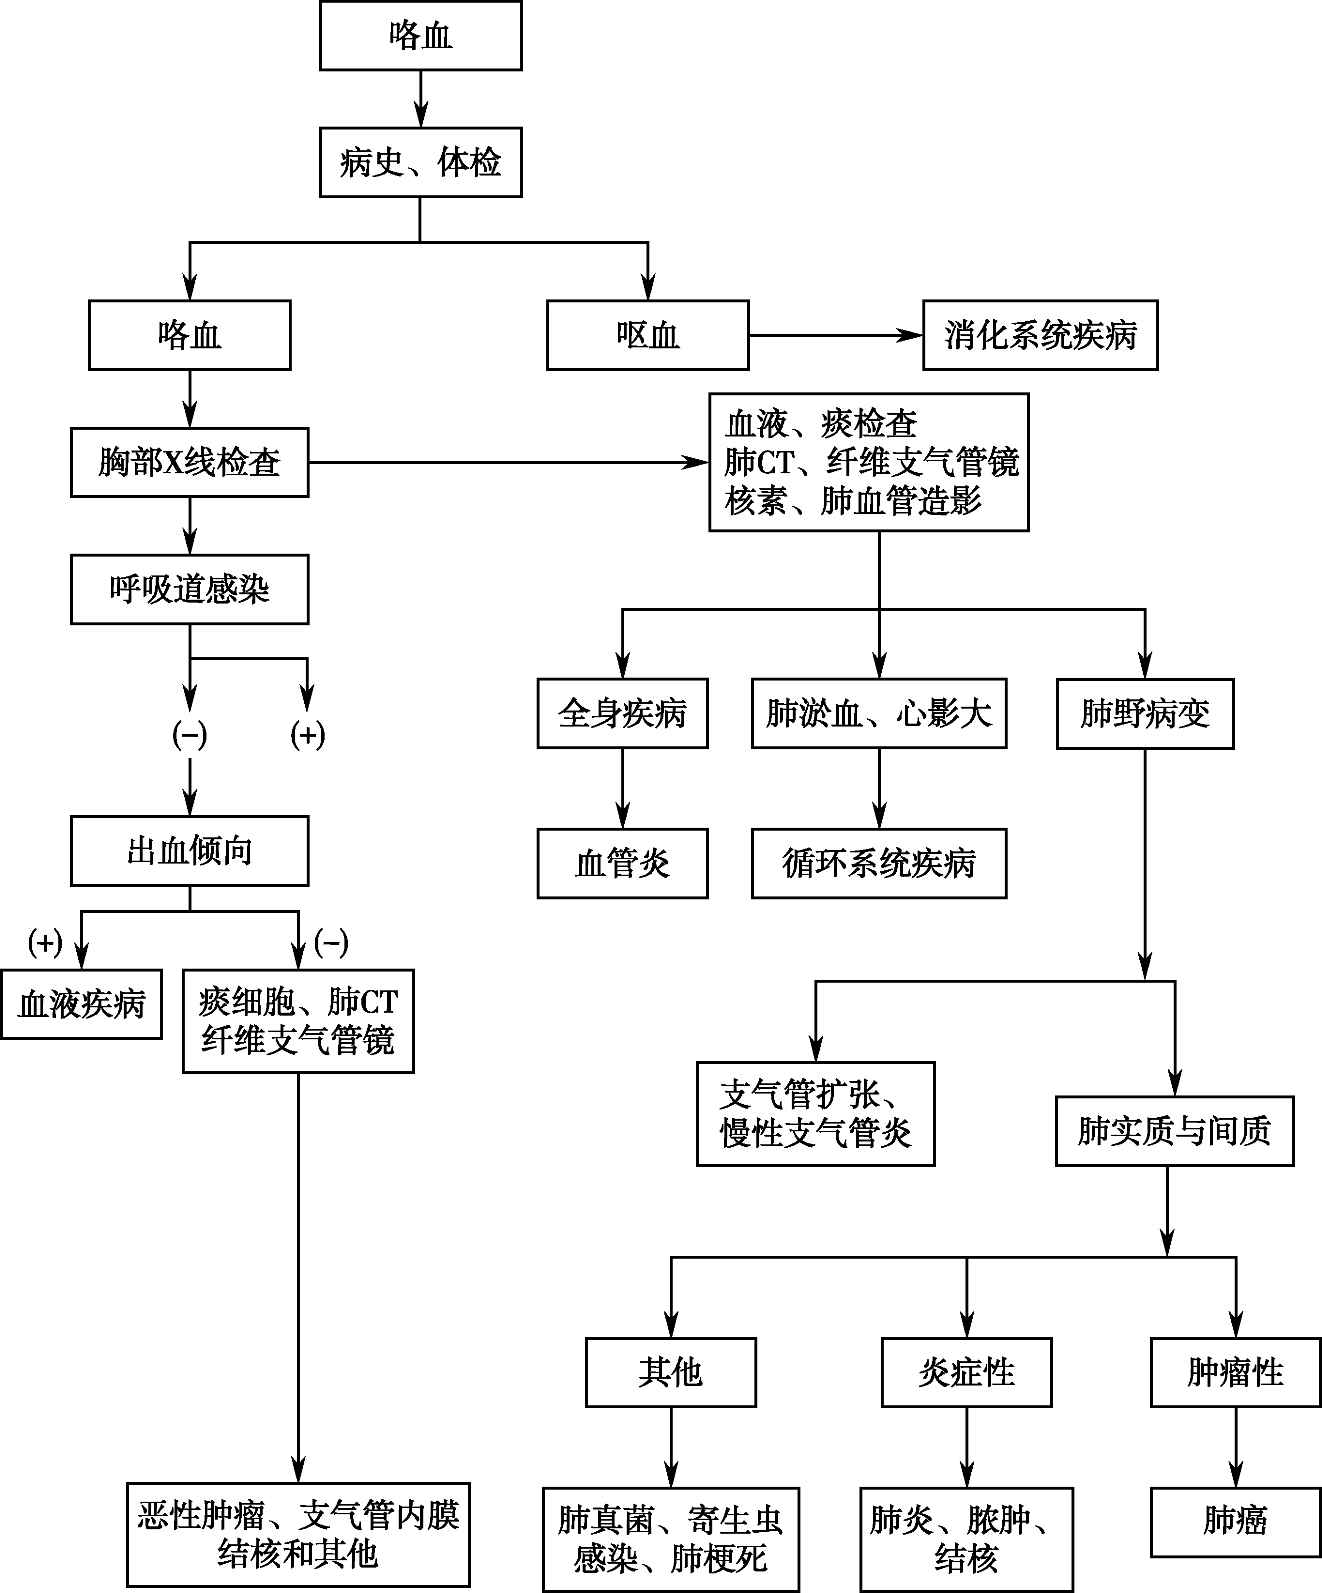
\includegraphics[width=4.55208in,height=5.47917in]{./images/Image00048.jpg}
 \captionsetup{justification=centering}
 \caption{咯血病因诊断流程图}
 \label{fig9-1}
  \end{figure} 

1.体位
患侧卧位,避免血液流向健侧。头低位,身体与床成40°~90°角,背部屈曲并拍击背部,促进肺内血液流出。病灶不明确者可暂取平卧位。同时清除口腔内血块。

2.保持呼吸道通畅
用导管自鼻腔插至咽喉部,用吸引器吸出血液(块),并刺激咽喉部,使患者用力咯出堵塞于气管内的血液(块),或在直接喉镜下作硬质支气管镜直接插管,通过冲洗和吸引,迅速恢复呼吸道通畅。

3.建立静脉通道 迅速建立静脉通道,补充血容量,使用止血药物,纠正休克。

4.镇静 根据病情需要,可适量给予镇静药物,如地西泮、氯丙嗪等。

5.机械通气 高浓度给氧(FiO\textsubscript{2}
30\%~40\%)或高频通气治疗。如自主呼吸微弱或消失,应立即进行气管插管或切开使用机械通气治疗。

6.若自主呼吸极弱或消失
,则应立即进行心肺复苏。在呼吸道通畅情况下同时使用呼吸兴奋剂。窒息解除后应及时对复苏后并发症进行处理,如纠正酸中毒、补充血容量、控制休克以及重要器官功能的监测与支持,如治疗和预防脑水肿、心肺功能不全、肾功能不全等。

大咯血患者应绝对卧床,尽量避免搬动或转送他院,颠簸可加重咯血,甚至导致死亡。如需转送,途中应将患者的头和身体偏向患侧或俯卧头低位,以利引流,防止窒息。密切观察患者的生命体征,包括意识、呼吸、脉搏和血压,随时做好抢救准备工作,尽可能准确记录咯血量。

\subsubsection{急诊处理}

\paragraph{镇静 、休息与对症处理}

少量咯血,如痰中带血,一般无需特殊处理,适当减少活动量,对症治疗即可。中等量咯血应卧床休息;大量咯血则应绝对卧床休息。取患侧卧位,患侧可放置冰袋,嘱患者将血轻轻咳出,避免吸入性肺炎、肺不张或以防窒息,出血部位不明时取平卧位。对精神紧张、恐惧不安者,应解除不必要的顾虑,必要时可给少量镇静药,如地西泮(安定)10mg或苯巴比妥钠0.1~0.2g肌注,或口服地西泮、氯氮{}
(利眠宁)等。鼓励患者咳出滞留于呼吸道的陈血,避免呼吸道阻塞。对频咳或剧咳者,可给镇咳药如喷托维林(pentoxyverine,咳必清)25mg,每天3次;可待因15~30mg,每天3次或二氧丙嗪(克咳敏)5mg,每天3次口服。但大咯血时一般不用镇咳剂,如剧咳妨碍止血,可在血液咳出后临时使用可待因15~30mg口服或皮下注射,每日1~3次;对年老体弱、肺功能不全者不宜用,禁用吗啡、哌替啶等,以免过度抑制咳嗽,使血液及分泌物淤积气道,引起窒息。

\paragraph{严密观察与护理}

进食易消化食物,保持大便通畅,避免用力屏气排便。对大、中量咯血者,应密切观察患者,做好大咯血与窒息的各项抢救准备,定期记录咯血量、测呼吸、脉搏和血压,若有口渴、烦躁、厥冷,面色苍白、咯血不止或窒息表现者,应立即进行抢救。

\paragraph{止血药物的应用}

常用止血药物有:

\hypertarget{text00024.htmlux5cux23CHP1-9-4-2-3-1}{}
(1) 垂体后叶素(pituitrin):

疗效迅速而显著,使肺循环压力降低,肺小动脉收缩而利于血凝块形成。用法:大咯血时以垂体后叶素5~10U加25\%葡萄糖液20~40ml缓慢静脉注射(10~15分钟);咯血持续者可用垂体后叶素10~20U加5\%葡萄糖液500ml,缓慢静滴;禁用于高血压、冠状动脉疾病、肺源性心脏病、心力衰竭患者和孕妇。注射过快可引起面色苍白、心悸、出汗、胸或腹痛、血压升高等副作用,应及时减慢速度或停药。

\hypertarget{text00024.htmlux5cux23CHP1-9-4-2-3-2}{}
(2) 普鲁卡因(procaine):

用于对垂体后叶素有禁忌者。普鲁卡因150~300mg加5\%葡萄糖液500ml缓慢静滴,或普鲁卡因50mg加25\%葡萄糖液40ml,缓慢静注。本药可诱发过敏反应,用药前应作皮试。药物使用量过大或注射过快,可导致惊厥、谵妄、兴奋、面色潮红,应立即停药,对症处理。

\hypertarget{text00024.htmlux5cux23CHP1-9-4-2-3-3}{}
(3) 酚妥拉明:

为α-肾上腺素能受体阻滞剂,能有效扩张血管平滑肌,降低肺循环阻力及心房压、肺毛细血管楔压和左心室充盈压,可起到较好的止血作用。酚妥拉明10~20mg加入5\%葡萄糖液250~500ml中持续静滴。使用时监测血压并保持有足够的血容量。

\hypertarget{text00024.htmlux5cux23CHP1-9-4-2-3-4}{}
(4) 纠正凝血障碍药物:

①6-氨基己酸(氨己酸,EACA):6.0g +
5\%葡萄糖液250ml静滴,通过抑制纤维蛋白溶酶形成达到止血目的,适用于肺部疾病、血液病引起的咯血。②氨甲苯酸(对羧基苄胺,PAMBA):100~200mg
+ 25\%葡萄糖液40ml静滴,或200mg +
5\%葡萄糖液500ml静滴,适用于纤维蛋白溶解亢进引起的出血。③氨甲环酸(AMCA):AMCA
250mg + 25\%葡萄糖液40ml静注;或AMCA 750mg +
5\%葡萄糖液500ml,静脉滴注。④肾上腺色腙(安络血):通过抑制毛细血管通透性、增加毛细血管抵抗和加速管壁回缩发挥止血作用。10~20mg肌肉注射,1日2次,或5mg
1日3次口服。⑤酚磺乙胺(止血敏):有收缩肺毛细血管、增加毛细血管抵抗、加速管壁回缩及轻微的促血小板聚集作用。0.25~0.75g肌肉注射或缓慢静脉注射,1日2~3次,静脉注射不宜过快,以免血压下降。⑥注射用血凝酶(立止血):该药对纤维蛋白原的降解有选择性作用,在出血部位生理性凝血因子的作用下,纤维蛋白多聚体迅速形成稳固的纤维蛋白,在出血部位发挥凝血作用。1~2U静脉注射或肌肉注射,1日1~2次。

\hypertarget{text00024.htmlux5cux23CHP1-9-4-2-3-5}{}
(5) 其他止血药物:

硝酸甘油适用于与垂体后叶素合用,5~10mg加入5\%~10\%葡萄糖液250~500ml中静滴;氯丙嗪能降低肺循环、左心室与支气管动脉压力,必要时可小剂量(10~15mg)配合使用,肝、肾功能不全者慎用。另外,阿托品、654-2、高渗氯化钠、糖皮质激素、中药如白连粉、三七粉、云南白药等、鱼精蛋白注射液、维生素C、凝血酶原复合物等根据病情均可酌情选用。

\paragraph{维持血容量}

持续大咯血出现循环容量不足时应及时补充血容量。输注新鲜血不但能补充血容量外,而且还有止血作用。

\paragraph{手术止血}

对反复咯血,上述治疗无效,出血部位明确而无手术禁忌者,可采用手术止血。指征包括:①肺部病变(如各型结核动脉破裂、支气管扩张、肺脓肿、肺癌等)所引起的致命性大咯血;②可能发生气道阻塞和(或)窒息者。

\paragraph{局部止血治疗}

适用于大咯血并发窒息和严重反复咯血、病情严重、肺功能较差、不适于手术治疗者。前提是出血部位明确,经气管插管或支气管镜边插边吸,到达出血部位后,将导管由活检孔插入至出血部位,注入冷生理盐水(4℃),每次50ml,留置30~60秒种后吸出,反复数次,直至出血停止,通过冷刺激使血管收缩达到止血的目的;或者注入凝血酶200~400U,或去甲肾上腺素液1~2mg稀释后局部使用。

\paragraph{支气管动脉栓塞}

对药物治疗无效且不能手术治疗的患者,是可选择的治疗方法之一。经股动脉插管,将漂浮导管插到病变区域支气管动脉分支的血管腔内,注入明胶海绵或聚乙烯醇微粒(直径0.5~2.0μm),栓塞支气管动脉,以达到止血目的。因肺循环可能有多支动脉供血,本法对不是来自支气管动脉(侧枝血管)破裂的咯血无效,而且造影剂和栓塞物还可能进入脊髓动脉,引起脊髓缺血损伤,因此应严格掌握适应证。

\paragraph{肺不张和肺炎的治疗}

采用体位引流(侧卧位,患侧在上),雾化吸入,使用解痉药、祛痰药,应用抗生素预防和控制感染。

\paragraph{病因治疗}

尽快明确病因,采用相应治疗措施。

\protect\hypertarget{text00025.html}{}{}

\hypertarget{text00025.htmlux5cux23CHP1-9-5}{}
参 考 文 献

1. Parrillo,Dellinger. Critical Care Medicine:Principles of Diagnosis
and Management in the Adult. 3th ed. Elsevier Inc,2008

2. Stone CK,Humphries. Current Emergency Diagnosis and Treatment. 5th
ed. New york:Lange/McGraw,2004

3. John A Marx. Rosen's Emergency Medicine. Concepts and Clinical
Practice. 6th ed. St. Louis:Mosby Inc,2006

4. 徐腾达,于学忠.现代急症诊断治疗学.北京:中国协和医科大学出版社,2007

5. 沈洪.急诊医学.北京:人民卫生出版社.2007

\protect\hypertarget{text00026.html}{}{}

\chapter{急 性 腹 痛}

腹痛(abdominal
pain)是指由于各种原因引起的腹腔内外脏器的病变,而表现在腹部的疼痛。可分为急性与慢性腹痛两类。急性腹痛(简称急腹痛)是临床最常见急症之一,其病因繁杂,病情多变,涉及学科广,内、外、妇产、儿及传染病等科疾病均可引起,诊断处理不当,常可造成恶果,因而对急性腹痛必须尽快作出定位、定性及病因诊断,以防误诊、漏诊及误治,从而改善预后。对生育期女性的急性腹痛须请妇产科医生会诊,以排除妇产科急腹症。

\subsection{病因与发病机制}

\subsubsection{病因}

引起腹痛的病因颇多,大体可分为腹腔内脏器疾病及腹腔外脏器疾病两大类,每类又可分为器质性病变及功能性失调;器质性病变包括脏器的急性炎症、损伤、破裂、穿孔、梗阻、扭转、出血、坏死等;功能性失调有痉挛、麻痹、神经功能紊乱及功能暂时性失调等(详见表\ref{tab10-1})。

\subsubsection{发病机制}

腹痛依发生机制分为三型,即真性内脏痛(true visceral
pain,内脏痛):由内脏本身病变所致;类似内脏痛(somatic
pain,体性痛,体壁性内脏痛):由内脏病变累及壁层腹膜,经躯体神经传入引起疼痛;放射痛(referred
pain,牵涉痛):内脏病变引起某一局部疼痛,痛处常非病变部位。

\paragraph{内脏痛}

多由消化道管壁平滑肌突然痉挛或强力收缩,管壁或脏器突然扩张,急性梗阻、缺血等刺激内脏传入神经末梢产生冲动所致,常为脏器本身的疼痛。

\paragraph{体性痛}

壁层腹膜分布着脊髓性感觉神经,脏层腹膜上虽无感觉受体,但近脏器的肠系膜、系膜根部、小网膜及膈肌等均有脊髓性感觉神经,当脏器病变累及其感觉神经时产生冲动,经上行传导达丘脑,再经交换神经元达大脑皮质。丘脑可感知疼痛,大脑可识别疼痛的部位、程度和性质。故体性痛多剧烈,疼痛及压痛部位明确,与体位有关,变换体位常可使疼痛增重。

\paragraph{放射痛}

亦称牵涉痛或感应性痛。由于某种病理情况致身体某一局部发生疼痛,且痛处常非病变所在,此因放射痛部位与病变脏器的感觉常来自同一节段神经纤维。放射痛的特点为常伴有Head皮肤感觉过敏带(内脏皮肤过敏带)及腹壁紧张。

Head皮肤过敏带即腹腔内脏器疾病的病理性冲动,刺激内脏神经经交感神经传入相应或同一脊髓段的后根,由此发出的脊神经产生感应,将冲动传到体表一定部位致皮肤相应节段感觉过敏性疼痛,或引起远隔部位脏器痛。如胆绞痛向右肩背部放射;小肠绞痛放射到脐周;胃、十二指肠病变可放射到剑脐间等。

\begin{table}[htbp]
\centering
\caption{急性腹痛的病因分类}
\label{tab10-1}
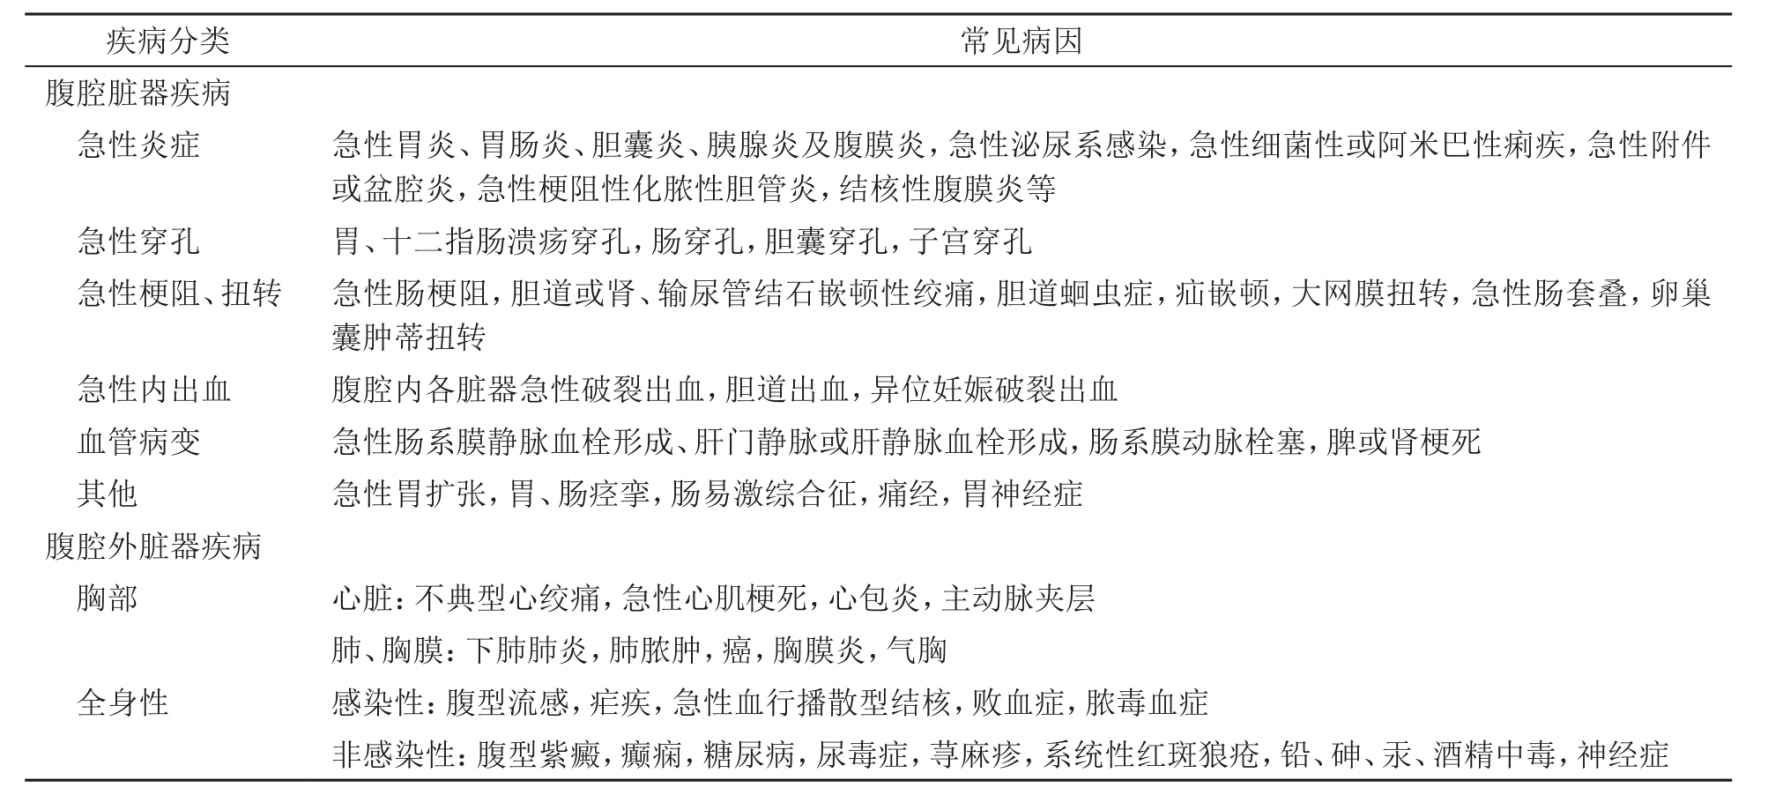
\includegraphics[width=6.67708in,height=3in]{./images/Image00050.jpg}
\end{table}

\subsection{诊断思路}

\subsubsection{病史及体检}

准确而简要的病史询问,全面而有重点的体检,对急性腹痛的诊断十分重要。

\hypertarget{text00026.htmlux5cux23CHP1-10-2-1-1}{}
(一) 年龄、性别、既往史

\paragraph{年龄 、性别}

不同年龄及性别常有不同的多发病,如婴幼儿多见先天性消化道畸形,尤其是胃肠道(肠闭锁或狭窄,肛门闭锁、先天性肥厚性幽门狭窄等)及胆道(先天性胆道闭锁或狭窄);幼儿多见肠寄生虫病、肠套叠、疝嵌顿等;青壮年多见急性阑尾炎、胃肠穿孔、肠梗阻、腹部外伤致脏器破裂内出血等;老年人则胃肠道癌肿及并发症(穿孔、梗阻、出血),胆结石或胆囊炎及血管疾病多见。急性胆道疾病、胰腺炎女多于男,溃疡病穿孔、急性阑尾炎及肠梗阻则男多于女。引起急性腹痛的妇产科疾病,如急性附件或盆腔炎,异位妊娠或破裂,卵巢囊肿蒂扭转,子宫破裂、穿孔等及痛经。

\paragraph{既往史}

应重点询问以往有否引起急性腹痛的病史,有无类似发作史;手术史、月经生产史、外伤史及有害物接触史等。

\hypertarget{text00026.htmlux5cux23CHP1-10-2-1-1-2-1}{}
(1) 有类似发作史者:

应考虑胆石症、胆囊炎、泌尿系结石、慢性阑尾炎或慢性胃炎急性发作,溃疡病活动或出血、穿孔,疝反复嵌顿,胃肠神经症等。

\hypertarget{text00026.htmlux5cux23CHP1-10-2-1-1-2-2}{}
(2) 手术史:

溃疡病胃次全切除术后吻合口溃疡、出血或狭窄,肠粘连或粘连性肠梗阻,膈下或盆腔脓肿等。

女性患者应注意有无痛经史,闭经且发生急性腹痛者应考虑异位妊娠、早期流产,若伴休克,应高度疑及异位妊娠破裂内出血等。

\hypertarget{text00026.htmlux5cux23CHP1-10-2-1-2}{}
(二) 注意腹腔内、外疾病所致急性腹痛的不同特点

\paragraph{腹腔内疾病急性腹痛的特点}

①常伴有消化道症状,如恶心、呕吐、腹泻、腹胀等。②常有与进食有关的诱因,如暴饮暴食、高脂饮食、酗酒、进食过刺激、不洁或变质食物等。③腹部体征较明显且固定(痛、压痛、叩痛、反跳痛等)。④无腹外及全身疾病表现。

\paragraph{外科或妇产科疾病所致急性腹痛的特点}

①腹痛突然发作,剧烈,急剧发展,不及时处理,短期内病情常迅速恶化。②表情痛苦,呻吟,大汗,面色苍白,辗转不安或蜷曲静卧。③可有腹膜刺激征(腹肌紧张呈板状,压痛、反跳痛明显)及肝浊音界缩小或消失。④可有内出血综合征,如头晕、心慌、多汗、面色苍白、脉细速、血压下降等。⑤急诊腹透可见膈下游离气体、高度胀气、鼓肠或胃扩张、梯形液气平面等。⑥发病短期内白细胞明显增高,中性及杆状核增高,中毒血象,进行性贫血等。

\paragraph{内科腹腔脏器疾病所致急性腹痛的特点}

①腹痛可轻可重,短期内病情不恶化。②症状与体征不一致,主观感觉腹痛剧烈,表情痛苦,但检查腹部体征不显著,多腹软,局部轻压痛或压痛,无反跳痛。③发病短期内血象正常或稍高,无中毒血象。④急诊腹透无阳性发现。

\hypertarget{text00026.htmlux5cux23CHP1-10-2-1-3}{}
(三) 依急性腹痛部位诊断

即依据解剖部位来推断可能的病因(表\ref{tab10-2})。最早发生腹痛及压痛最明显的部位常是发生病变的部位(早期及异位阑尾炎例外)。

\hypertarget{text00026.htmlux5cux23CHP1-10-2-1-4}{}
(四) 依病史、体征及伴随症状综合分析

\paragraph{起病方式}

突然发作剧痛,多为胆道蛔虫症、胆道或泌尿道结石嵌顿、疝嵌顿、急性胆囊炎或胰腺炎、消化道急性穿孔、腹腔脏器破裂、急性心肌梗死、心绞痛等。持续性腹痛阵发性加重常示有痉挛或梗阻;初期呈进行性加重多为急性炎症;暴饮暴食、高脂饮食、酗酒、过刺激或不洁食物、激烈运动等诱发急性腹痛应考虑急性胆囊炎、胰腺炎或胃肠炎,溃疡病穿孔,肠或卵巢囊肿蒂扭转,疝嵌顿等。

\paragraph{绞痛及放射痛}

\begin{table}[htbp]
\centering
\caption{急性腹痛部位与疾病关系}
\label{tab10-2}
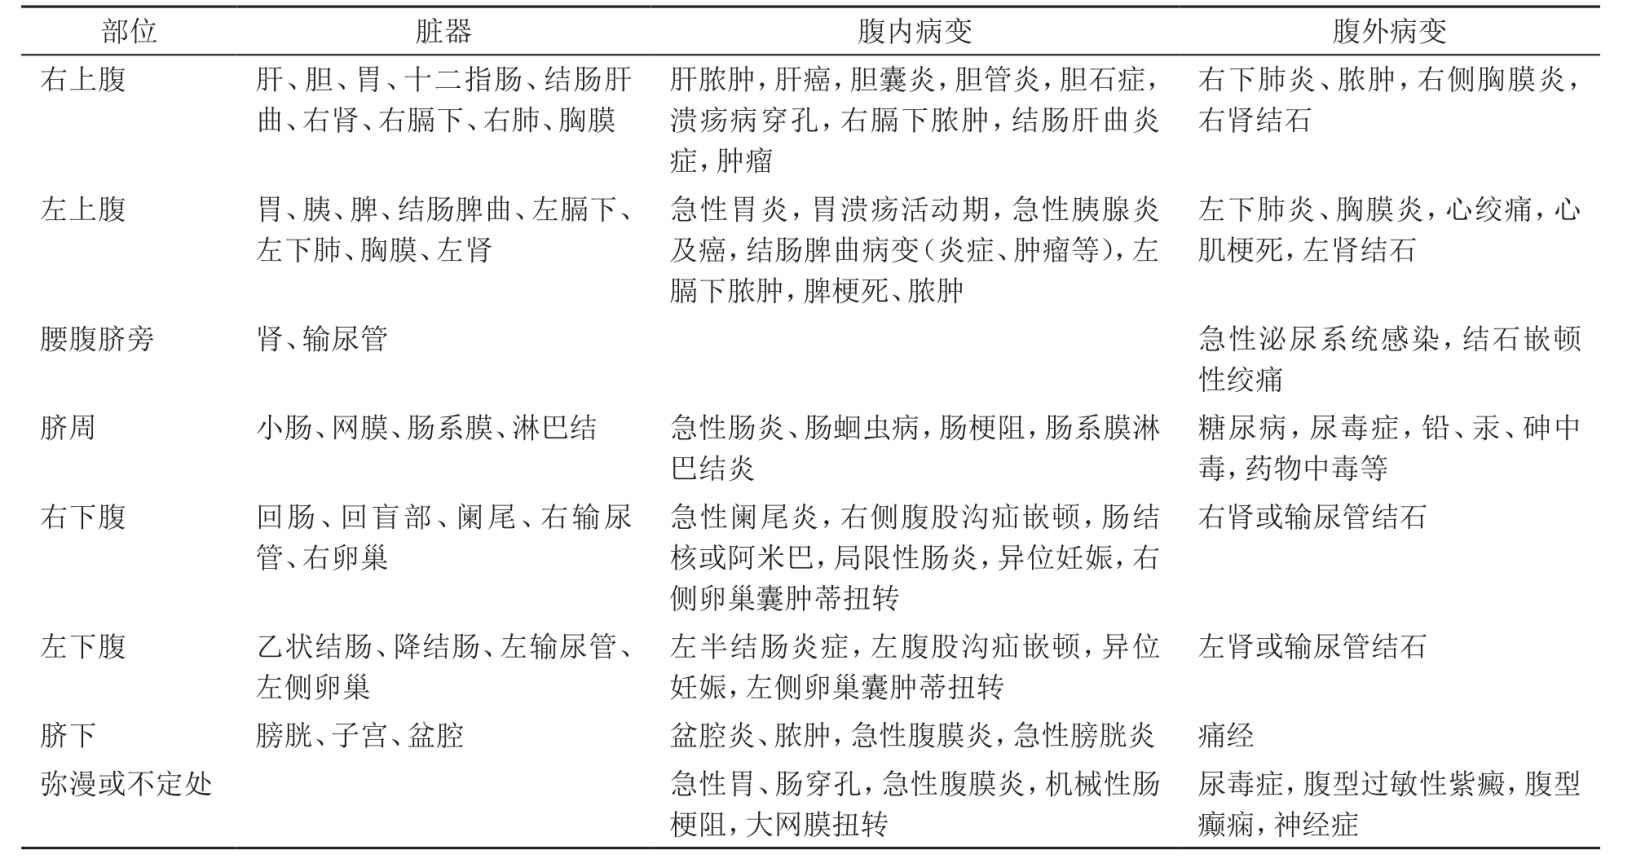
\includegraphics[width=6.71875in,height=3.52083in]{./images/Image00051.jpg}
\end{table}

①胆绞痛:右上腹痛向右肩胛及右背部放射。②胰腺绞痛:上腹或中上腹部向左侧腰背部放射。③小肠绞痛:脐周剧痛。④肾绞痛:肾区痛沿腹直肌外缘向大腿内侧或会阴部放射。⑤子宫或直肠病变绞痛:腰骶部或下腹部剧痛或坠痛。

\paragraph{伴发症状}

\hypertarget{text00026.htmlux5cux23CHP1-10-2-1-4-3-1}{}
(1) 伴发热:

①先发热后腹痛多为不需手术治疗的内科性疾病(常为急性炎症)。②先腹痛后发热的多为外科或妇产科疾病,且常需手术治疗(如急性消化道穿孔、腹膜炎、肠梗阻、异位妊娠破裂、内脏破裂出血等)。③急性腹痛伴寒战、高热,应考虑急性化脓性胆囊炎、胆管炎,腹腔或腹内脏器的化脓性病变(膈下或盆腔脓肿、化脓性腹膜炎),下肺炎症或脓肿等。

\hypertarget{text00026.htmlux5cux23CHP1-10-2-1-4-3-2}{}
(2) 伴呕吐:

急性腹痛伴呕吐者常为急性胃、胆囊、胰腺等炎症,肠梗阻,胆道或泌尿道结石嵌顿,胃型感冒,肠套叠,痛经,神经症等。

\hypertarget{text00026.htmlux5cux23CHP1-10-2-1-4-3-3}{}
(3) 与排便的关系:

①腹痛伴腹泻:急性肠炎、痢疾、急性盆腔炎、急性阑尾炎、高位肠梗阻等。②腹痛伴血便:绞窄性肠梗阻、肠套叠、溃疡性结肠炎、坏死性肠炎、缺血性疾病(栓塞或血栓形成)等。③腹痛伴便秘或停止排便及肛门排气:为习惯或非习惯性便秘、肠梗阻等。

\hypertarget{text00026.htmlux5cux23CHP1-10-2-1-4-3-4}{}
(4) 伴腹胀:

急性胃扩张、麻痹性肠梗阻、便秘、尿潴留等。

\hypertarget{text00026.htmlux5cux23CHP1-10-2-1-4-3-5}{}
(5) 伴黄疸:

①右上腹痛伴黄疸者多为肝、胆系统疾病(炎症、结石、肿瘤等)。②中上腹或左中上腹痛伴黄疸多为胰腺(炎症、结石、肿瘤)或脾脏病变(脾梗死)。③右上腹痛伴寒战、高热、黄疸,应考虑急性胆囊炎,胆结石嵌顿伴炎症,急性化脓性胆囊、胆管炎,急性肝脓肿及少数膈下脓肿。

\hypertarget{text00026.htmlux5cux23CHP1-10-2-1-4-3-6}{}
(6) 与排尿关系:

腹痛伴膀胱刺激征或血尿者多为急性泌尿系感染、结石嵌顿;部分阑尾炎、盆腔脓肿也可引起膀胱刺激征,应注意鉴别。

\hypertarget{text00026.htmlux5cux23CHP1-10-2-1-4-3-7}{}
(7) 与体位的关系:

①辗转不安,腹痛喜按多为胃肠道疾病;拒按多为肝、胆系疾病。②活动疼痛加剧,蜷曲侧卧疼痛减轻多为腹膜炎。③前倾坐位或膝胸位疼痛减轻多为胰腺疾病。

\hypertarget{text00026.htmlux5cux23CHP1-10-2-1-4-3-8}{}
(8) 伴腹水:

①伴血性腹水:腹腔内脏或异位妊娠破裂,恶性肿瘤腹腔内转移,腹膜恶性肿瘤,少数结核性渗出性腹膜炎等。②脓性腹水:化脓性腹膜炎。③胰性腹水:乳糜状,浆液或浆液血性,淀粉酶含量增高且大于血中含量,蛋白量增高,对利尿剂及放腹水疗效差,见于急性出血坏死型胰腺炎或胰腺假囊肿破裂。④胆汁性腹水:化脓性胆囊炎或胆管炎破裂致胆汁性腹膜炎。

\hypertarget{text00026.htmlux5cux23CHP1-10-2-1-4-3-9}{}
(9) 伴休克:

应考虑下列疾病:①急性内出血:腹腔内脏器破裂或异位妊娠破裂。②急性穿孔致弥漫性腹膜炎。③腹腔内脏器或卵巢囊肿蒂扭转。④腹腔内急性血管性病变(肠系膜动脉栓塞或静脉血栓形成)。⑤急性心肌梗死或休克型肺炎。

\hypertarget{text00026.htmlux5cux23CHP1-10-2-1-4-3-10}{}
(10) 伴包块:

应考虑相应部位的急性炎症、肿瘤、肠套叠或扭转。

\hypertarget{text00026.htmlux5cux23CHP1-10-2-1-4-3-11}{}
(11) 与外伤关系:

急性腹痛发生前有外伤史者应考虑腹腔脏器破裂、内出血等。

\subsubsection{辅助检查}

\paragraph{血液检查}

①血红蛋白及红细胞计数:可提示有无内出血致贫血(但早期由于脾脏及骨髓代偿性释放以及血液浓缩,可显示不出贫血或与临床实际贫血程度不符)。②白细胞计数及分类:可提示是否感染、感染程度等。

\paragraph{大便检查}

外观:颜色、性状(成形、糊状、水样、血便、脓血便、黏液便或脓血黏液便等)。镜检:有无红、白细胞,虫卵、真菌、阿米巴滋养体等及潜血试验。

\paragraph{尿液检查}

尿pH、蛋白、糖、酮体、胆红素、红细胞、白细胞、管型、细菌、真菌等,育龄女性应查尿妊娠试验。

\paragraph{生化检查}

依病情需要可作:①血、尿淀粉酶测定;②血钾、钠、氯、钙,血糖,酮体等测定;③肝、肾功能测定等。

\paragraph{心电图检查}

对40岁以上患者,既往无慢性胃病史,突然发作上腹痛应常规作心电图,以识别有无心脏及心包病变。

\paragraph{X线检查}

①胸部X线检查:有助于肺炎、肺脓肿、肺癌、胸膜炎、气胸、肝或膈下脓肿等的诊断。②腹部X线检查:消化道急性穿孔致膈下游离气体,肠梗阻的梯形液气平面,急性胃扩张,高度鼓肠等。另外,胆道或泌尿道阳性结石等。

\paragraph{超声波检查}

B超检查对肝、胆、胰、脾、肾、输尿管、子宫及其附件、盆腔、腹腔等探查均有较强分辨(实质性、囊性、良性、恶性、积液、结石等)及诊断能力,对胃肠道疾病可提供一定的诊断线索。

\paragraph{内镜检查}

急诊内镜检查(胃、十二指肠、胆道、腹腔及结肠镜检查),对急性腹痛的诊断具有极其重要意义。可依临床初步拟诊病变部位,选择相应内镜检查,以助诊断及内镜直视下取活检或治疗。

\paragraph{腹部}

CT检查
主要检查肝、胆、胰、脾、肾、膀胱、腹腔及盆腔等部位,可诊断其形态、大小、密度、占位性病变(实质性、囊性)、结石及腹腔、盆腔有无积液、肿大淋巴结等。

\paragraph{诊断性腹腔穿刺术}

根据穿刺液性质可确定腹膜炎性质,有无内出血(脏器破裂或异位妊娠破裂)等。

\paragraph{阴道后穹隆穿刺术}

主要用于判断异位妊娠破裂出血、盆腔脓肿或盆腔积液。

\subsubsection{急性腹痛的病因诊断线索}

急性腹痛的病因繁多。为尽早明确诊断,应在完成病史采集、体格检查和必要的辅助检查之后,对所得资料进行综合分析,作出正确的病因诊断。下述诊断思路,有助于最终确定病因诊断。

\hypertarget{text00026.htmlux5cux23CHP1-10-2-3-1}{}
(一) 确定是腹腔内病变或腹腔外病变

急性腹痛的诊断 ,首先要确定是腹腔内病变还是腹腔外病变。

\paragraph{腹腔内病变}

常有消化道症状如恶心、呕吐、腹痛、腹泻等,腹痛程度不一,多有较明确诱因。腹部体征依病因而异,一般较明显,腹外与全身性症状轻微或缺乏。

\paragraph{腹腔外病变}

胸部疾病引起的腹痛位于脐上的同侧腹部,可有压痛,但一般无反跳痛及肌紧张,胸部检查可发现有关疾病的心肺体征,胸部X线检查、心电图检查、心肌酶学检查等有助于诊断。全身性疾病所致的腹痛有原发病的表现,腹痛多由于电解质紊乱、代谢失调或毒素刺激所致,位于全腹或部位多变,一般无腹膜刺激征。

\hypertarget{text00026.htmlux5cux23CHP1-10-2-3-2}{}
(二) 确定是外科或非外科急性腹痛

\paragraph{外科急性腹痛}

是指急需外科处理,或病情的发展有需要外科处理可能性的急性腹痛。对急性腹痛患者,应先明确是否为外科急性腹痛。此类腹痛常有以下特点:①剧烈而急起的腹痛多先于发热或呕吐,发热多于腹痛后4~6小时出现,但细菌性肝脓肿、脾脓肿和伤寒肠穿孔等例外。若腹痛超过6小时而患者体温反而降低或低于正常,则应考虑并发休克、大出血或严重感染毒血症的可能。②腹痛部位明确,有固定区,患者多“拒按”腹痛区。③常伴腹膜刺激征。腹痛、固定性压痛点和肌紧张的程度常是越来越严重,提示病变呈进行性发展。④腹式呼吸减弱或消失,肠鸣音亢进或消失,机械性肠梗阻时可闻及高调肠鸣音,而弥散性腹膜炎、麻痹性肠梗阻则肠鸣音减弱或消失。⑤可有肝肺浊音界消失,腹部移动性浊音阳性。⑥腹痛时腹部膨隆或可见胃肠型及蠕动波,并可触及腹部包块或索状物等。⑦腹腔穿刺可有血性或脓性液体等。

\paragraph{内科急性腹痛}

其特点:①一般先有发热或呕吐、腹泻而后出现腹痛。②腹痛可轻可重,腹部体征不明显,无固定而局限性压痛点,无腹膜刺激征。患者常喜按。③腹式呼吸存在,肠鸣音正常或活跃。④可有与腹痛有关的内科疾病的阳性体征。⑤血白细胞正常或升高。

\paragraph{妇产科急性腹痛}

其特点:①由于女性生殖器官集中于下腹部盆腔内,所以妇产科疾病引起的腹痛多局限于中下腹、盆腔,并向会阴和骶尾部放射。②腹痛多与月经、妊娠有关,月经期曾患过上呼吸道感染或有过性生活,多为急性盆腔炎;卵泡破裂多发生在排卵期;宫外孕有停经史,可有早孕反应等。③可伴有腹腔内出血、阴道出血或分泌物增加。④妇科检查常有阳性体征发现。

\paragraph{小儿内科急性腹痛}

其特点:①常以发热、咽痛、咳嗽等症状先于腹痛。②急性腹痛而腹壁柔软,无压痛,腹部无包块、肠型等腹部体征。③腹痛范围广,不规则性,但排便基本正常。④可伴有呕吐等。⑤腹部外疾病引起腹痛者,可发现原发病变部位的阳性体征。

\hypertarget{text00026.htmlux5cux23CHP1-10-2-3-3}{}
(三) 确定急性腹痛的性质

根据常见的病变性质可将急性腹痛归纳为以下七类:

\paragraph{炎症性急性腹痛}

基本特点为:腹痛+发热+压痛或腹肌紧张。

临床特点有:①一般起病较缓慢,多由轻渐重。②持续性腹痛。因脏器或腹膜的炎症、充血、水肿,刺激神经而引起急性腹痛,多呈持续性腹痛进行性加重。因发病的部位、病变程度及其病理变化不同,而呈局限性或全腹性疼痛。疼痛多发生于病变所在的部位。③当炎症病变波及脏器浆膜和壁层腹膜时,则呈典型的局限性或弥漫性腹膜刺激征,即腹肌紧张、压痛和反跳痛,尤其是以病变所在部位最明显。④早期可出现全身感染征象,如寒战、发热、脉快和白细胞增高。⑤腹腔穿刺和灌洗可抽出腹腔炎性渗出物。⑥可有明显的胃肠道刺激症状。此类急腹痛常见的有急性阑尾炎、急性胆囊炎、急性腹膜炎、急性胰腺炎、急性盆腔炎、急性肠系膜淋巴结炎、急性出血性坏死性肠炎等。

\paragraph{穿孔性急性腹痛}

基本特点是:突发持续腹痛+腹膜刺激征,可伴有肠鸣音消失或气腹。

由外伤、炎症或癌肿侵蚀等导致空腔脏器破裂所致。其临床特点有:①突然剧烈的刀割样腹痛,后呈持续性,范围迅速扩大。②腹壁板样强直,有明显腹膜刺激征,常伴有休克。③常见膈下游离气体和腹部移动性浊音。④肠鸣音消失。例如消化性溃疡穿孔、胃癌穿孔、胆囊穿孔、伤寒肠穿孔、外伤性肠穿孔等。

\paragraph{梗阻性急性腹痛}

基本特点是:阵发性腹痛+呕吐+腹胀+排泄功能障碍。

肠道、胆道、输尿管等空腔管道内结石、肿瘤和位置改变(如扭转、套叠)等因素阻塞,腔内压增高促使管腔道平滑肌强烈收缩以排除障碍,发展到血运障碍(如绞窄性疝等),或始发于血运障碍(如肠系膜血管阻塞等),继发缺血、坏死等变化,即发生梗阻性急腹痛。其临床特点有:①阵发性腹部剧痛是其特征,多突然发生,呈阵发性剧烈绞痛,往往使患者难以忍受。当梗阻器官合并炎症或血运障碍时,常呈持续性腹痛,阵发性加重。②恶心、呕吐,早期是反射性,后期是逆流性呕吐。因梗阻发生的部位不同,呕吐的内容和量亦不同。胃肠道高位梗阻则早发频吐,多为胃及十二指肠内容物;低位梗阻则晚发溢吐,严重者可呕吐粪性内容物。③腹胀和梗阻的器官管型明显,此因梗阻的器官、部位、程度和病变性质不同而表现亦异:如幽门梗阻表现上腹胀、振水音,可见胃蠕动波;肠梗阻可见腹胀、肠型、蠕动波;胆道梗阻出现胆囊肿大或胆管扩张;泌尿系梗阻出现膀胱区域或肾区的囊性肿块等。④正常排泄功能障碍。胃肠道梗阻出现呕吐、肛门停止排便排气;胆道梗阻出现黄疸;泌尿系梗阻则呈现尿少或尿潴留、肾积水等。⑤除泌尿系疾病外,多伴有水、电解质与酸碱平衡失调、休克,或晚期毒血症。此类急性腹痛常见的有肾、输尿管结石、肝内胆管结石、肝外胆管结石、胆绞痛、胆道蛔虫病、肠梗阻、肠套叠、嵌顿性腹股沟疝、嵌顿性股疝、卵巢囊肿蒂扭转等。

\paragraph{出血性急性腹痛}

其基本特点是:腹痛+失血性休克与急性贫血+隐性(内)出血或显性(外)出血(呕血、便血或尿血)。

腹内实质脏器或血管因外伤或病变发生破裂引起腹腔内出血,由于大量积血刺激导致急性腹膜炎,但腹膜刺激症状较轻,无感染症状,而有急性失血症状。临床特点有:①可有肝癌、消化性溃疡、腹主动脉瘤、输卵管妊娠以及肝、脾外伤等病史。②起病较急骤,腹痛为持续性,但不及炎症性或穿孔性腹痛剧烈。③外观可见的出血,如呕血、便血、尿血等,或胃肠吸引、导尿、肛管直肠或阴道内诊等证实有内出血者。④虽无外观出血,但证实有内出血:进行性贫血;腹部有移动性浊音,腹腔穿刺抽出不凝固的血液。⑤有失血性休克表现。⑥B超可探及腹腔内液性暗区及受损伤的脏器。此类急性腹痛常见的有消化性溃疡出血、外伤性肝脾破裂出血、胆道出血、肝癌破裂出血、腹主动脉瘤破裂大出血、异位妊娠破裂出血等。

\paragraph{损伤性急性腹痛}

其基本特点是:外伤+腹痛+腹膜炎或内出血综合征。

腹部损伤,因暴力及着力点不同,可有腹壁伤,如挫伤、肌肉撕裂伤、腹壁血肿形成;空腔脏器伤,如胃、小肠、大肠、胆囊、膀胱破裂等;以及实质性脏器伤,如肝、脾、胰、肾损伤等。临床特点有:①有外伤史,尤其是腹部、腰部和下胸部外伤。②腹痛,原发性休克恢复后,常呈现急性持续性剧烈腹痛,伴恶心、呕吐。③内出血征象:烦躁不安、面色苍白、出冷汗、口渴、脉搏细速、血压进行性下降,重者出现休克;腹部有移动性浊音,腹穿可抽出新鲜或暗红色不凝固的血液。④腹膜炎综合征:恶心、呕吐、腹痛、腹肌紧张,压痛、反跳痛明显;腹穿抽出物可为消化道分泌物或腹性分泌物。⑤X线检查:腹内脏器移位、阴影扩大或消失、膈下游离气体、腹内积液或积气。

\paragraph{绞窄与扭转性急性腹痛}

这是由于肠道(如小肠、乙状结肠)、较活动的脏器(如游离的脾、肾等)、有蒂肿瘤(如卵巢囊肿)、腹内、外疝等发生扭转及绞窄,引起缺血、组织坏死和血性渗液,亦称缺血性急腹痛。临床特点有:①腹痛为持续性,因受阵发牵拉,可有阵发性类似绞痛的加剧。②常可触及压痛性包块。③早期无腹膜刺激征,随着坏死的发生而出现。④可有频繁干呕,消化道排空症状如频繁便意,排气,也可排出肠道黏液或黏液血便等。

\paragraph{功能性紊乱及全身性疾病所致的急性腹痛}

临床特点有:①常有精神因素或全身性疾病史。②腹痛常无明确定位,呈间歇性、一过性或不规则性。③腹痛虽严重,但体征轻,腹软,无固定压痛和反跳痛。如食管弥漫性痉挛、胆道运行功能障碍、结肠肝(脾)曲综合征、游走肾、肠道易激综合征、胃肠神经症等;全身性疾病如肠系膜动脉硬化或缺血性肠病,结缔组织病累及胃肠道、血卟啉病、腹型癫痫、过敏性紫癜等。

\subsection{处理原则}

\subsubsection{急性腹痛的处理原则}

\paragraph{快速评估}

迅速检查呼吸、脉搏、血压、神志和体温,把急性腹痛分为三类:①危重:先救命后治病。如腹主动脉瘤破裂、异位妊娠破裂并重症休克等。要在快速纠正休克的同时急诊手术或介入治疗控制出血。②重:诊断与治疗相结合。如绞窄性肠梗阻、消化道穿孔、卵巢囊肿蒂扭转等。要在尽快完成各项有关检查的同时,纠正一般情况,准备急诊手术和相关治疗。③普通(可有潜在危险性):寻找危及生命潜在原因。如胃肠炎、消化道溃疡、慢性炎症、腹壁神经性或肌肉疼痛,也可能是恶性肿瘤,结石等。按常规诊疗程序进行采集病史、体格检查、辅助检查、诊断、鉴别诊断。

\paragraph{急性腹痛病因未明者}

对病因不明的急性腹痛患者,应密切观察,辅以必要的辅助检查,以尽早作出诊断,同时给予积极的对症支持疗法。

\hypertarget{text00026.htmlux5cux23CHP1-10-3-1-2-1}{}
(1) 严密观察护理、有目的有计划地追踪诊断:

对诊断不明的急性腹痛患者,切忌主观片面、放任自流,应认真做到“三严”,即严肃追踪观察、严密护理和严格做好临床交接班工作,尤其是对下述情况更应该提高警惕:①特殊的阑尾炎,如老、幼、孕妇或异位阑尾炎;②易被忽略的妇女嵌顿性斜疝或股疝;③绞痛后尚可排便的肠梗阻,如肠套叠、不全肠梗阻或高位肠梗阻;④外伤史很轻或无外伤史的自发性肝、脾破裂,肝或脾包膜下血肿继发大出血等;⑤无胃病史或无气腹的消化性溃疡穿孔、出血,早期症状轻的小穿孔或穿孔后暂时好转期的患者;⑥多发性损伤患者,尤其是易被忽略的并发闭合性腹部损伤;⑦某些病史不详的患者如休克、昏迷和婴幼儿等。对这类患者,必须严密追踪观察病情变化,多次重复检查与估计病情,以便尽早明确诊断,指导治疗。动态观察的重点内容有:①生命体征:体温、脉搏、呼吸、血压和神志的变化;②腹部情况:腹痛的部位、性质、范围、程度以及腹膜刺激征的变化等;③心、肺、肝、肾、脑等重要脏器的功能变化;④胃肠道功能状态:饮食、呕吐、腹泻、排便情况、腹胀、肠蠕动、肠鸣音等;⑤腹腔的异常,如腹腔积气、积液、肝浊音界变化和移动性浊音;⑥新的症状与体征的出现等。严密观察期间,应禁食、禁忌止痛、禁用泻药、禁止灌肠等“四禁”。其目的是为了避免加重病情,防止掩盖症状而妨碍临床观察病情变化,防治并发症。若病情必须使用镇痛剂,可先试用阿托品、654-2等抗胆碱药物,严禁使用吗啡、哌替啶(度冷丁)等麻醉剂。但近年来有学者研究认为,早期正确有效地使用止痛剂不仅可以较大程度地减轻患者的疼痛,不影响患者的诊断和治疗,还有助于患者配合各项检查,提高诊断的准确性。

\hypertarget{text00026.htmlux5cux23CHP1-10-3-1-2-2}{}
(2) 对症支持疗法:

①纠正水、电解质紊乱;②抗感染:对有发热、白细胞总数及中性粒细胞增高的炎症性疾病患者,及时使用有效抗生素对疾病转归有积极作用;③防治腹胀:通常采用的措施是禁饮食,持续有效的胃肠减压等;④防止休克等。

\hypertarget{text00026.htmlux5cux23CHP1-10-3-1-2-3}{}
(3) 剖腹探查指征:

①疑有腹腔内出血不止;②疑有肠坏死或肠穿孔而有严重腹膜炎;③经密切观察和积极治疗后,腹痛不缓解,腹部体征不减轻,全身情况无好转反而加重。

\paragraph{急性腹痛的病因明确者}

立即作病因治疗(包括手术治疗等)。如对肠梗阻、内脏穿孔或出血、急性阑尾炎等有手术指征者,应及时手术治疗。对腹痛能忍受者一般不用镇痛剂,但对病因已明确而不需手术治疗、疼痛较剧的患者,应适当使用镇痛剂,有利于病情恢复。可根据腹痛的性质与程度选用药物,如肝胆胰疾病或输尿管结石所致的疼痛多采用吗啡、哌替啶与阿托品合用;消化性溃疡疼痛宜用抗酸、解痉剂及H\textsubscript{2}
受体阻滞剂等抗溃疡药物治疗;功能性腹痛多用解痉剂和精神安定剂等。急性腹痛的处理程序见图\ref{fig10-1}。

\subsubsection{常见急性腹痛危重情况的诊治}

\paragraph{急性腹痛伴失血性休克}

\hypertarget{text00026.htmlux5cux23CHP1-10-3-2-1-1}{}
(1) 临床表现特点:

①交感兴奋症状:精神紧张、脉快、苍白、额头冷汗、手指冰冷;②末梢循环障碍:甲床青紫、当压迫患者甲床和耳垂后毛细血管再充盈缓慢;轻压患者的前臂时,患者的手背静脉不易充盈、尿少等;③脉搏细速、血压下降;④中心静脉压和心脏排出量降低。

\hypertarget{text00026.htmlux5cux23CHP1-10-3-2-1-2}{}
(2) 治疗原则:

①积极进行抗休克治疗。②需要进行紧急剖腹手术以控制出血。

\begin{figure}[!htbp]
 \centering
 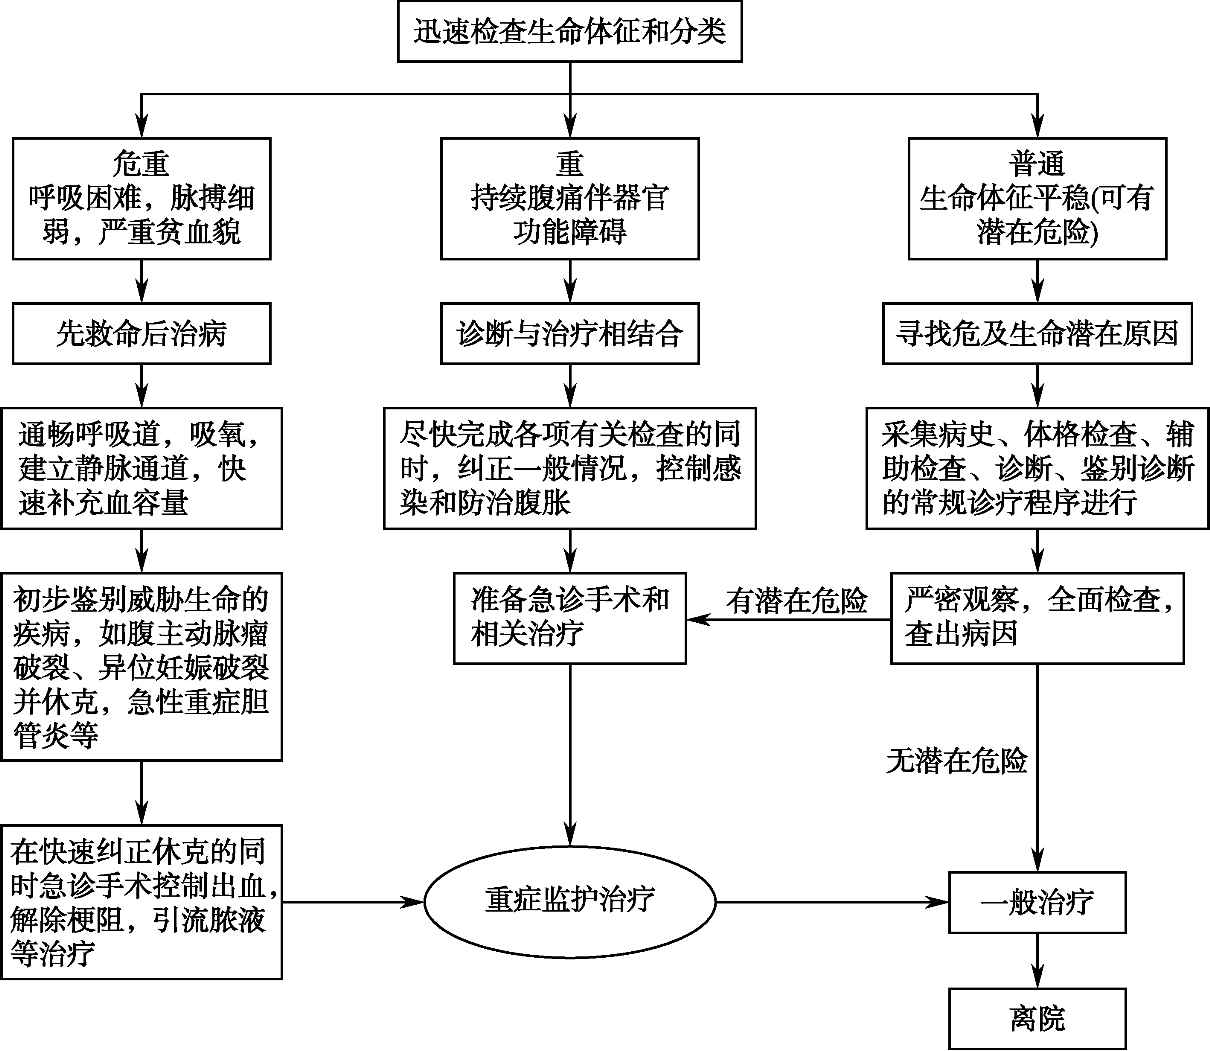
\includegraphics[width=4.71875in,height=4.10417in]{./images/Image00052.jpg}
 \captionsetup{justification=centering}
 \caption{急性腹痛的处理程序}
 \label{fig10-1}
  \end{figure} 

\paragraph{急性腹痛伴感染性休克}

\hypertarget{text00026.htmlux5cux23CHP1-10-3-2-2-1}{}
(1) 临床表现特点:

①重度中毒表现如寒战,体温迅速升高,精神萎靡,意识障碍等;②休克征象表现为面色苍白,血压下降、尿量减少,脉搏细速,末梢循环不良等;③白细胞明显升高或低于正常甚至核左移。

\hypertarget{text00026.htmlux5cux23CHP1-10-3-2-2-2}{}
(2) 治疗原则:

①扩充血容量,静脉输液;②给予抗生素治疗;③物理方法降温;④寻找感染灶的可能部位并及时处理。

\paragraph{继发性急性腹膜炎}

继发性急性腹膜炎是指由各种腹腔内病变或外伤所继发的腹膜急性炎症。

\hypertarget{text00026.htmlux5cux23CHP1-10-3-2-3-1}{}
(1) 临床表现特点:

①最突出的症状是腹痛,多为突然发病;常表现为持续性、烧灼样疼痛,随身体的活动而加剧。在炎症最明显处疼痛最重。疼痛范围缩小、程度减轻时,提示炎症局限;反之,则表明炎症扩散。②其他常见症状包括恶心、呕吐、食欲不振、口渴和自觉发热等,发病后患者多表现为尿少和便秘。③急性腹膜炎的特异性体征------腹膜刺激征:肌紧张、压痛和反跳痛。④中毒症状:疾病的早期,患者的体温往往增高并不明显,随着病程的进展,患者体温可以逐渐增高到38℃以上。甚至出现中毒性休克。⑤在空腔脏器穿孔的病例,可出现气腹征------肺肝界叩不清或消失,腹透时隔下有游离气体。⑥腹部穿刺:对诊断非常有帮助。通过对吸出的腹腔液性状进行观察,常可以判断出腹膜炎的病因。

\hypertarget{text00026.htmlux5cux23CHP1-10-3-2-3-2}{}
(2) 治疗原则:

①动态监测患者的病情变化、胃肠减压并留置尿管导尿;②补充血容量、应用抗生素;③积极处理原发病,及时手术处理。

\protect\hypertarget{text00027.html}{}{}

\hypertarget{text00027.htmlux5cux23CHP1-10-4}{}
参 考 文 献

1. 高德明 ,吴金生.现代急腹症学.北京:人民军医出版社,2002

2. Lo Vecchio F,Oster N,Sturmann K,et al. The use of analgesics in
patient with acute abdominal pain. J Emerg Med,1997,15 (6):775

3.
周玲君,刘红香,赵继军.急腹症的早期止痛.中华急诊医学杂志,2006,15(1):91

4. Lo Vecchio F,Oster N,Sturmann K,et al. The use of analgesics in
patient with acute abdominal pain. J Emerg Med,1997,15 (6):775

5. 刘保池 .急腹症的正确诊断与处理.国际外科学杂志,2008,35(6):369

\protect\hypertarget{text00028.html}{}{}

\chapter{恶心与呕吐}

恶心(nausea)、呕吐(vomiting)是临床上常见的症状之一。恶心是一种特殊的主观感觉,表现为胃部不适和胀满感,常为呕吐的前奏,多伴有迷走神经兴奋的症状,如皮肤苍白、流涎、出汗、血压降低及心动过缓等;呕吐是一种胃的反射性强力收缩,通过胃、食管、口腔、膈肌和腹肌等部位的协同作用,能迫使胃内容物由胃、食管经口腔急速排出体外。从某种意义上来说呕吐是机体的一种保护性作用,它可把对机体有害的物质排出体外,但实际上很多呕吐并非摄入有害物质引起,而且频繁和剧烈的呕吐,可引起失水、电解质紊乱和营养障碍。

\subsection{病因与发病机制}

\subsubsection{病因}

引起恶心、呕吐的病因很广泛,包括多方面因素,几乎涉及各个系统。

\paragraph{感染}

病毒性急性胃肠炎、细菌性急性胃肠炎、急性病毒性肝炎、阑尾炎、胆囊炎、腹膜炎、急性输卵管炎、盆腔炎等。

\paragraph{腹腔其他脏器疾病}

①脏器疼痛:胰腺炎、胆石症、肾结石、肠缺血、卵巢囊肿蒂扭转。②胃肠道梗阻:幽门梗阻(溃疡病、胃癌、腔外肿物压迫)、十二指肠梗阻(十二指肠癌、胰腺癌)、肠粘连、肠套叠、绞窄疝、克罗恩病、肠结核、肠道肿瘤、肠蛔虫、肠扭转、肠系膜上动脉压迫综合征、输出袢综合征、胃肠动力障碍(糖尿病胃轻瘫、非糖尿病胃轻瘫)、假性肠梗阻(结缔组织病、糖尿病性肠神经病、肿瘤性肠神经病、淀粉样变等)。

\paragraph{内分泌代谢性疾病}

低钠血症、代谢性酸中毒、营养不良、维生素缺乏症、糖尿病酸中毒、甲状腺功能亢进、甲状腺功能低下、甲状旁腺功能亢进症、垂体功能低下、肾上腺功能低下,各种内分泌危象、尿毒症等。

\paragraph{神经系统疾病}

中枢神经系统感染(脑炎、脑膜炎)、脑肿瘤、脑供血不足、脑出血、颅脑外伤、脑寄生虫病等。

\paragraph{药物等理化因素}

麻醉剂、洋地黄类、化疗药物、抗生素、多巴胺受体激动药、非甾体抗炎药、茶碱、酒精、放射线等。

\paragraph{精神性呕吐}

神经性多食、神经性厌食。

\paragraph{前庭疾病}

晕动症、梅尼埃病、内耳迷路炎。

\paragraph{妊娠呕吐}

妊娠剧吐、妊娠期急性脂肪肝。

\paragraph{其他}

心肺疾患(心肌梗死、肺梗死、高血压、急性肺部感染、肺心病)、泌尿系疾患(急性肾炎、急性肾盂肾炎、尿毒症)、周期性呕吐、术后恶心呕吐、青光眼。

\subsubsection{发病机制}

这是一系列复杂的反射动作,可分为三个阶段,即恶心、干呕与呕吐。恶心发生时,唾液分泌增加,胃蠕动减弱或者消失、排空延缓,十二指肠及近端空肠紧张性增加,出现逆蠕动,导致十二指肠内容物反流至胃内。干呕时胃上部放松而胃窦部短暂收缩;呕吐时胃窦部持续收缩,下食管括约肌松弛,腹肌收缩,膈肌下降,腹压增加,迫使胃内容物急速而猛烈地从胃反流,经食管、口腔而排出体外。呕吐与反食不同,后者系无恶心与呕吐的协调动作而使胃内容物一口一口地反流到口腔。

目前认为的主要的反射通路包括:①信息传入:由自主神经传导(其中迷走神经纤维较交感神经纤维起的作用大)。②呕吐反射中枢:目前认为中枢神经系统的两个区域与呕吐反射密切相关。一是延髓呕吐中枢,另一是化学感受器触发区(chemical
trigger zone,CTZ)。③传出神经:包括迷走神经、交感神经、体神经和脑神经。

通常把内脏末梢传来的冲动引起的呕吐称为反射性呕吐,把CTZ受刺激后引起的呕吐称为中枢性呕吐。延髓呕吐中枢位于延髓外侧网状结构背外侧,迷走神经核附近,主要接受来自消化道和内脏神经、大脑皮质、前庭器官、视神经、痛觉感受器和化学感受区的传入冲动。化学感受器触发区(CTZ)位于第四脑室底部的后极区,为双侧性区域,有密集多巴胺受体。多巴胺受体在CTZ对呕吐介导过程中起重要作用,因为应用阿扑吗啡、左旋多巴、溴隐亭等多巴胺受体激动药可引起呕吐,而其拮抗药、甲氧氯普胺(胃复安)、吗丁啉等药物有止呕作用。化学感受器触发区的5-羟色胺、去甲肾上腺素、神经肽物质和γ-氨基丁酸等神经递质也可能参与呕吐反射过程。CTZ主要接受来自血液循环中的化学、药物等方面的呕吐刺激信号,并发出引起呕吐反应的神经冲动。但CTZ本身不能直接引起呕吐,必须在延髓呕吐中枢完整及其介导下才能引起呕吐,但两者的关系尚不十分明确。CTZ位于血-脑脊液屏障之外,许多药物或代谢紊乱均可作用于CTZ。某些药物如麻醉剂、化学药物、麦角衍生物类药、吐根糖浆等及体内某些多肽物质如甲状腺激素释放激素、P物质、血管紧张素、胃泌素、加压素、血管肠肽等均可作用于CTZ引起恶心呕吐。此外,某些疾病如尿毒症、低氧血症、酮症酸中毒、放射病、晕动症等引起的恶心呕吐也与CTZ有关。

传出神经的呕吐信号传至效应器官,引起恶心呕吐过程,呕吐开始时,幽门关闭,胃内容物不能排到十二指肠,同时,贲门口松弛,贲门部上升,腹肌,膈肌和肋间肌收缩,胃内压及腹内压增高,下食管括约肌松弛,导致胃内容物排出体外。

\subsection{诊断思路}

\subsubsection{病史}

\paragraph{药物或放射线接触史}

易引起呕吐的常用药物有某些抗生素、洋地黄、茶碱、化疗药物、麻醉剂、酒精等。镭照射线治疗和钴照射线治疗,常引起恶心呕吐。

\paragraph{其他}

呕吐可为许多系统性疾病的表现之一,包括糖尿病、甲状腺功能亢进症或甲状腺功能减退症、肾上腺功能减退等内分泌疾病、硬皮病等结缔组织病、脑供血不足、脑出血、脑瘤、脑膜炎、脑外伤等中枢神经系统疾病、尿毒症等肾脏疾病。

\subsubsection{临床表现特点}

\paragraph{呕吐的伴随症状}

呕吐伴发热者,须注意急性感染性疾病;呕吐伴有不洁饮食或同食者集体发病者,应考虑食物或药物中毒;呕吐伴胸痛,常见于急性心肌梗死或急性肺梗死等;呕吐伴有腹痛者,常见于腹腔脏器炎症、梗阻和破裂;腹痛于呕吐后暂时缓解者,提示消化性溃疡、急性胃炎及肠道梗阻性疾病;呕吐伴头痛,除考虑颅内高压的疾患外,还应考虑偏头痛、鼻炎、青光眼及屈光不正等疾病;呕吐伴眩晕,应考虑前庭、迷路疾病、基底椎动脉供血不足、小脑后下动脉供血不足及某些药物(氨基糖苷类抗生素)引起的脑神经损伤。

\paragraph{呕吐的方式和特征}

喷射性呕吐多见于颅内炎症、水肿出血、占位性病变、脑膜炎症粘连等所致颅内压增高,通常不伴有恶心。此外,青光眼和第Ⅷ对脑神经病变也可出现喷射性呕吐。呕吐不费力,餐后即发生,呕吐物量少,见于精神性呕吐。应注意呕吐物的量、颜色和气味等。呕吐物量大,且含有腐烂食物提示幽门梗阻伴胃潴留、胃轻瘫及小肠上端梗阻等;呕吐物为咖啡样或血性见于上消化道出血,含有未完全消化的食物则提示食管性呕吐(贲门失弛缓症、食管憩室、食管癌等)和见于神经性呕吐、胆囊炎、胆石症及胃大部切除术后等,有时见于妊娠剧烈呕吐、晕动症;呕吐物有酸臭味者,或胃内容物有粪臭味提示小肠低位梗阻、麻痹性肠梗阻、结肠梗阻而回盲瓣关闭不全或胃结肠瘘等。

\paragraph{呕吐和进食的时相关系}

进食过程或进食后早期发生呕吐,常见于幽门管溃疡或精神性呕吐;进食后期或餐后呕吐,见于幽门梗阻、肠梗阻、胃轻瘫或肠系膜上动脉压迫导致十二指肠雍积;晨起呕吐多见于妊娠呕吐,有时亦见于尿毒症、慢性酒精性中毒和颅内高压等。

\subsubsection{体格检查}

\paragraph{一般情况}

应注意神志、营养状态、有无脱水、循环衰竭、贫血及发热等。

\paragraph{腹部体征}

应注意胃型、胃蠕动波、振水声等幽门梗阻表现:肠鸣音亢进、肠型等急性肠梗阻表现:腹肌紧张、压痛、反跳痛等急腹症表现。此外,还应注意有无腹部肿块、疝等。

\paragraph{其他}

①眼部检查注意眼球震颤、眼压测定、眼底有无视乳头水肿等。②有无病理反射及腹膜刺激征等。

\subsubsection{实验室检查}

主要包括与炎症、内分泌代谢及水盐电解质代谢紊乱等有关的实验室检查。

\subsubsection{其他辅助检查}

可做B超、胃镜、ERCP、超声内镜、CT、磁共振等特殊检查。

\subsection{治疗}

由于引起恶心、呕吐的疾病很多,恶心、呕吐仅是疾病的症状之一。因此,在未明确病因之前不应盲目应用作用于呕吐中枢的强镇吐药物,否则会贻误病情。只有在明确了导致呕吐的病因之后,在积极治疗病因的基础上,才能行必要的对症治疗。

\paragraph{胃肠道疾病}

包括食管、胃、十二指肠直至空肠、回肠、结肠及直肠在内的任何部位的病变都有可能引起恶心、呕吐的症状,其中以食管狭窄、食管癌、贲门失弛缓、贲门癌、胃窦部嗜酸性肉芽肿、胃窦部巨大溃疡或癌肿、十二指肠溃疡或郁积症、多种原因导致的小肠与大肠梗阻或急性胃、小肠或大肠的炎症性病变为最常见的病因。因消化道良性或恶性病变造成的狭窄或梗阻所致的呕吐,药物治疗是无效的,只有经扩张、置入支架或手术治疗,解除狭窄或梗阻之后,呕吐症状才会消失。对于贲门失弛缓症患者,在未进行扩张或手术治疗之前,可选用钙离子通道拮抗药或硝酸甘油餐前半小时口服或餐前15~30分钟舌下含化治疗,早期可改善呕吐及梗阻症状:或者试用肉毒杆菌毒素行狭窄局部注射治疗。胃肠道急性炎症性病变引起的呕吐,应积极选用抗生素并纠正电解质紊乱及补充维生素;胃肠动力障碍引起的恶心与呕吐则可应用莫沙比利(mosapride,5mg口服,每日3次)、西沙比利(cisapride,5~10mg口服,每日2~4次)、多潘立酮(吗丁啉,10~20mg口服,每日3次;或10mg肌肉注射)、甲氧氯普胺(灭吐灵,胃复安,5~10mg口服;或10~20mg肌肉注射。每日剂量应≤0.5mg/kg,否则易引起锥体外系反应)等促胃肠动力剂;如果呕吐是由胃肠道痉挛所致,则可应用东莨菪碱(0.3mg口服或注射)等抗胆碱能药物。

\paragraph{肝脏 、胆道及胰腺疾病}

是导致恶心、呕吐的常见病因之一。恶心、呕吐可是急性病毒性肝炎的早期症状,常与食欲减退、厌油腻食物及上腹部饱胀同时出现,随着护肝治疗及适当的休息之后,恶心与呕吐可逐渐消失。呕吐也是胆道梗阻或绞痛常伴随的症状,只有当胆道梗阻或炎症消除之后,呕吐才会停止;急性胰腺炎时常伴随有恶心与呕吐症状,只有随着采用胃肠减压、减少胰液分泌等措施之后,呕吐才会逐步缓解或终止。

\paragraph{中枢神经系统病变}

包括各种原因所致的脑炎、脑膜炎、脑肿瘤、脑寄生虫病、脑血管病及颅脑外伤等病变,均可引起颅内压力增高而导致恶心、呕吐。治疗的重要措施之一就是应用降低颅内压、减轻脑细胞水肿的药物治疗。脱水治疗后,不仅可改善呕吐的症状,更重要的是起到了保护或恢复脑细胞功能的作用。

\paragraph{药物所致的呕吐}

多种药物有引起恶心与呕吐的不良反应,一般而言,只要立即停止应用引起呕吐的药物,呕吐症状就会减轻直至消失,因此并不需要应用镇吐类药物。目前临床上对某些恶性肿瘤或血液系统的恶性疾病(如白血病、恶性淋巴瘤、多发性骨髓瘤、恶性组织细胞病等)采用联合化疗或放疗,或对某些恶性肿瘤采用抗癌药物行介入治疗。但无论在治疗过程中或治疗之后,均可引起较为严重的胃肠道不良反应,最突出的表现就是恶心与呕吐。为了预防或减轻此不良反应,常可应用镇吐药物进行治疗,常用的药物有昂丹司琼(ondansetron,奥丹西龙,商品名:枢复宁。常用8mg口服或静脉注射)、格拉司琼(granisetron,商品名:康泉。成人剂量每次40μg/kg,或标准剂量3mg,静脉滴注)等。必须指出,应用这些作用强的镇吐药物之后,也会产生中枢神经系统、心血管系统或胃肠道的不良反应,故应严格控制药物剂量及间隔时间。

\paragraph{神经 、精神因素所致的呕吐}

对此类原因所致的呕吐,心理治疗是关键。首先应消除患者的精神心理障碍,其次可配合药物治疗,常用的药物是镇静药与胃肠促动力剂、重者可采用多塞平或氟西汀等抗抑郁药物治疗。禁忌应用昂丹司琼(奥丹西龙)等强烈作用的镇吐药。

\protect\hypertarget{text00029.html}{}{}

\hypertarget{text00029.htmlux5cux23CHP1-11-4}{}
参 考 文 献

1. 陈文彬,潘祥林.诊断学.第7版.北京:人民卫生出版社,2008

2. 陈新谦,金有豫,汤光.新编药物学.第17版.北京:人民卫生出版社,2011

\protect\hypertarget{text00030.html}{}{}

\chapter{急 性 腹 泻}

正常人一般每日排成形大便1次,粪便平均重量为150~200g,一般不超过200g,其中水分占60\%~70\%,约150ml左右。少数人每天排便2~3次或2~3天才排1次,但若粪质成形,性状与常人无异,亦属正常。

腹泻(diarrhea)是指排便习惯和粪便性状发生变化,排便次数增多(每天3次以上),粪质稀薄,水分增加(水分超过85\%),粪便量增加(超过200g/d)。便质不成形、稀溏或呈液状,有时含有脓血或带有未消化食物及脂肪。确定是否有腹泻应根据个体的大便习惯而异。

腹泻可根据病程分为急性腹泻和慢性腹泻两种,也可依病因分为感染性腹泻和非感染性腹泻两大类。急性腹泻是指起病急骤、病程较短,病程在2~3周之内,极少超过6~8周。慢性腹泻指病程至少在4周以上,常超过6~8周,或间歇期在2~4周内的复发性腹泻。腹泻常伴有排便紧迫感、肛门不适或大便失禁。腹泻可导致水电解质丢失,严重时可引起大量失水,导致低血容量性休克和急性器官功能衰竭,甚至因电解质严重紊乱引起严重心律失常而死亡。

\subsection{病因与发病机制}

在禁食期间,正常人肠腔内液体含量很少。但正常三餐摄取后,每天约有9L液体进入肠道,其中2L来自进食的食物和饮料,其余来自消化道分泌液,包括唾液1.5L、胃液2.5L、胰液1.5L、胆汁0.5L和小肠液1.0L。进入胃肠道的食糜在通过小肠时,食糜的渗透度变得与血浆相同,其中90\%的水分被其吸收。食糜在到达回肠末端时,已呈等渗状态,每天仅有1~2L的液体进入结肠,而结肠也具有强大的吸收水分的功能,使大便最终含水量只有100~200ml。若胃肠道的分泌、消化、吸收和运动等功能障碍,使消化道分泌的液量增加,食物不能完全分解,吸收量减少和肠胃蠕动加速等,最终可导致粪便性状稀薄、次数增加而形成腹泻。腹泻的发病机制相当复杂,从病理生理角度分为四类,部分腹泻的发病可有几个因素并存,具体如下:

\paragraph{分泌性腹泻}

肠道液体主要由黏膜隐窝细胞分泌,大部分经肠绒毛腔面上皮细胞吸收。当各种刺激因子刺激肠黏膜细胞分泌的量超过其吸收能力时,所引起的腹泻称分泌性腹泻(secretory
diarrhea)。刺激肠黏膜分泌的因子可分为四类:①细菌的肠毒素,如霍乱弧菌、大肠埃希菌、沙门菌等毒素;②神经体液因子,如血管活性肠肽(VIP)、血清素、降钙素等;③免疫炎性介质,如前列腺素、白三烯、血小板活化因子、肿瘤坏死因子、白介素等;④去污剂,如胆盐和长链脂肪酸,通过刺激阴离子分泌和增加黏膜上皮通透性而引起分泌性腹泻;⑤各种通便药,如蓖麻油、酚酞、芦荟、番泻叶等均可引起分泌性腹泻。

肠道分泌电解质和水分的机制相当复杂。近年发现,肠黏膜隐窝细胞中的第二信使如环磷酸腺苷(cAMP)、环磷酸鸟苷(cGMP)、钙离子等的增加是诱导黏膜隐窝细胞分泌的重要环节。霍乱弧菌和致病性大肠埃希菌的毒素首先与上皮细胞刷状缘上的受体结合,激活腺苷环化酶-cAMP系统,致cAMP浓度增高,引起大量肠液分泌;艰难梭菌(C.difficile)是通过钙离子增加而引起分泌性腹泻;血管活性肽瘤(VIP瘤)引起的腹泻是一种非感染性的分泌性腹泻,肿瘤释出的VIP能激活肠黏膜的腺苷酸环化酶,刺激小肠大量分泌液体,故而出现霍乱样的严重水泻,称为胰性霍乱,常伴有严重的低钾血症和代谢性酸中毒;胃泌素瘤能分泌大量的胃泌素,刺激壁细胞分泌大量胃液,过多胃液进入小肠后,不仅可损害空肠黏膜,而且促进肠道蠕动,使胰脂肪酶灭活,脂肪消化障碍而更加重腹泻。分泌性腹泻还可见于直肠分泌性绒毛状腺瘤、肠淋巴瘤、炎症性肠病、肠肉芽肿性疾病、结缔组织病、恶性类癌综合征、甲状腺髓样癌等。

分泌性腹泻的特点是:①禁食不减轻腹泻;②肠液与血浆的渗透压相同;③大便呈水样,量多,无脓血;④一般不伴有腹痛;⑤肠黏膜组织学基本正常。

\paragraph{渗透性腹泻}

由于肠腔内含有大量不能被吸收的溶质,导致肠腔内渗透压升高,大量液体被动进入肠腔而引起腹泻,称为渗透性腹泻(osmotic
diarrhea)或吸收不良性腹泻(malabsorption diarrhea)。见于:

\hypertarget{text00030.htmlux5cux23CHP1-12-1-2-1}{}
(1) 高渗性药物:

口服镁盐、乳果糖、甘露醇或山梨醇等高渗性药物。

\hypertarget{text00030.htmlux5cux23CHP1-12-1-2-2}{}
(2) 高渗性食物:

主要是某些碳水化合物,由于水解酶缺乏或其他原因而导致食物吸收不良,形成高渗透压性的肠内容物而引起腹泻。临床上最常见的是原发性乳糖酶缺乏,患者口服牛奶或奶制品后即可引起腹泻。

\hypertarget{text00030.htmlux5cux23CHP1-12-1-2-3}{}
(3) 消化不良:

胃大部分切除术后、萎缩性胃炎和胃癌患者的胃液分泌减少,慢性胰腺炎、胰腺切除术后使胰液分泌减少,严重肝病或胆管梗阻可导致胆汁分泌或排泄减少,使食物不能充分被消化,营养物质不能被吸收,致使高渗性肠内容物增多而造成腹泻。

\hypertarget{text00030.htmlux5cux23CHP1-12-1-2-4}{}
(4) 吸收不良:

①黏膜透过性异常:由于小肠黏膜细胞的特殊病变如绒毛或微绒毛的变形、萎缩等变化,导致小肠的有效吸收面积缩小和黏膜透过水和电解质减少而导致腹泻。见于小儿乳糜泻、热带和亚热带斯泼卢等疾病。②肠吸收面积减少:如小肠切除后等。③肠黏膜充血、水肿:由于门静脉内压力增加,引起肠道黏膜广泛充血与水肿,影响肠道内营养物质的吸收而发生腹泻。④细菌繁殖过多:在某些疾病状态下,如肝硬化、小肠浸润性疾病引起的部分性肠梗阻或某些小肠失蠕动(如系统性硬皮病)、盲袢等,小肠内细菌可以过多繁殖。由于细菌分泌的毒素可影响消化酶的作用,以及细菌分解物结合胆盐,使其失去形成微胶粒的能力,导致脂肪等食物的消化和吸收受到障碍等,可引起腹泻或脂泻。⑤吸收抑制:如先天性氯泻(congenital
chloriderrhea),是由于氯的主动吸收功能不全而钠的吸收过程正常,以致肠内容物中由于氢和氯化物增加,但缺乏碳酸氢钠与之中和而使肠液呈酸性,回肠和结肠内液体积聚而引起腹泻。氯泻也可继发于长期腹泻而缺钾的患者。

渗透性腹泻的特点是:①当引起腹泻的原因除去(如禁食)之后,腹泻即可停止或减轻;②肠腔内的渗透压可超过血浆渗透压;③粪中含有大量未被完全吸收或消化的食物。

\paragraph{肠动力紊乱(motility disturbances)}

许多药物、疾病和胃肠道手术可改变肠道的正常运动功能,促使肠蠕动加速,以致肠内容物过快通过肠腔,因影响消化与吸收而发生腹泻。肠动力过缓亦可导致腹泻,其原因为结肠型的细菌在小肠定植和过度生长,从而使脂肪、胆盐和碳水化合物的吸收受到影响。此类腹泻可见于淀粉样变性、硬皮病、糖尿病性神经病变、胃大部切除术后、幽门或肛门括约肌切除术后、肠易激综合征、情绪性腹泻、毒性甲状腺肿病、恶性类癌综合征等。

此种腹泻的特点是粪便稀烂或水样,肠鸣音亢进,常伴有腹痛,但大便中很少有炎症细胞。

\paragraph{渗出性腹泻(exudative diarrhea)}

又称炎症性腹泻(inflammatory
diarrhea)。肠黏膜炎症时渗出大量黏液、脓、血,可致腹泻。此类腹泻可见于:①炎症性肠病,如克罗恩病和溃疡性结肠炎;②感染性炎症:来自侵入性病原体及其毒素,如志贺痢疾杆菌、沙门菌属、弯曲杆菌、耶尔森菌(Yersinia)、结核杆菌、阿米巴原虫、艰难梭菌等的感染;③缺血性炎症;④肠放射损伤;⑤嗜酸性肠炎:为嗜酸性粒细胞浸润胃肠道全层,可累及全胃肠道或节段性,表现为脂肪泻、腹痛、恶心、呕吐、消瘦,外周血嗜酸性粒细胞可增多。

渗出性腹泻的特点是:①粪便松散或水样,含有黏液和脓血,左侧结肠病变所致者常带有肉眼可见的脓血便,小肠病变一般无肉眼可见的脓血便。②腹泻和全身症状、体征的严重程度因肠受损程度而异。

需要指出和值得注意的是,同一种疾病产生的腹泻常常有多种机制参与,且腹泻的病因并不单纯,可同时或先后有几个病因并存。临床上最常见的为各种肠道感染、炎症、结肠和直肠癌、葡萄球菌肠毒素所引起的食物中毒及肠道易激综合征等。

\subsection{诊断思路}

腹泻的病因诊断要依靠病史、症状、体征,并结合辅助检查,尤其是粪便检验的结果,综合分析后得出结论。对一时难以明确诊断者,可进一步作X线钡剂检查和(或)结肠镜检查;对胆、胰疾病可选用超声、CT、MR、逆行胰胆管造影(ERCP)等影像学诊断方法加以明确诊断;对小肠吸收不良者可行小肠吸收功能试验、呼气试验、小肠黏膜活检等以明确诊断。但在诊断过程中应注意以下几点。

\subsubsection{病史}

\paragraph{年龄与性别}

婴幼儿起病的腹泻,应考虑先天性小肠消化吸收障碍性疾病,如双糖酶缺乏症、先天性氯泻等。病毒性胃肠炎和大肠埃希菌性肠炎多见于婴幼儿;细菌性痢疾以儿童和青壮年多见;结肠癌多见于中年或老年;阿米巴痢疾则以成年男性居多;功能性腹泻、甲亢和滥用泻剂者多见于女性,而结肠憩室与结肠癌则多见于男性。

\paragraph{起病与病程}

需询问国际、国内和郊区旅游史、近期服用了哪些药物或免疫抑制剂、是否亲密接触动物等。急性腹泻均应注意询问接触或摄入不洁食物史、起病与演变过程等。急性食物中毒性感染常于进食后2~24小时内发病;手术后发病,尤其是长期接受抗生素治疗者,应考虑金黄色葡萄球菌肠炎、难辨梭状芽胞杆菌性肠炎等。由功能性腹泻、血吸虫病、溃疡性结肠炎、克罗恩病等所引起的腹泻,可长达数年或数十年。功能性腹泻、吸收不良综合征和结肠憩室炎所致的腹泻,常呈间歇性的发作。

\paragraph{排便与粪便性状}

往往可以提示病变部位或性质。腹泻量多、水样、色淡、多泡沫、恶臭、无脓血、无里急后重,提示病变位于小肠;黏液带果酱色血便,病变多在上段结肠;粉红色脓血便,病变多在下端结肠;粪便表面带血或伴明显里急后重,病变多在直肠。急性腹泻先为水样后为脓血便,一日多至数十次,伴有里急后重者急性细菌性痢疾的可能性较大;粪便暗红色、酱色状或血水样,提示阿米巴痢疾可能;粪便稀水样,无里急后重,多为食物中毒性感染;若在进食后6~24小时发病则以沙门菌属、变形杆菌、产气荚膜梭状芽胞杆菌感染的可能性大;若在进食后2~5小时发病,伴有剧烈呕吐者可能为金黄色葡萄球菌感染所致。呕吐物和腹泻均呈米泔水样,失水严重,应考虑霍乱;若粪便带有恶臭,呈紫色血便,应考虑急性出血性坏死性肠炎。吸收不良综合征时粪便有食物残渣、未消化或发酵物,可奇臭;结肠炎症引起的腹泻粪便带脓血;肠结核和肠易激综合征常有腹泻与便秘交替现象。肠易激综合征的功能性腹泻多在清晨起床后和早餐后发生,每日2~3次,粪便有时含大量黏液。影响睡眠的夜间腹泻多系器质性疾病所致。

\paragraph{腹泻与腹痛}

腹泻伴有里急后重且下腹或左下腹持续性腹痛,腹痛于便后可稍减轻,提示病变位于直肠或乙状结肠;腹泻无里急后重,伴脐周腹痛为小肠性腹泻。

\paragraph{伴随症状}

急性腹泻伴有高热,以细菌性痢疾、沙门菌属食物中毒感染居多;有里急后重以细菌性痢疾、阿米巴痢疾、急性血吸虫病可能性大,而食物中毒性感染大多无里急后重。

\subsubsection{体格检查}

对腹泻患者应做全面仔细的体格检查。如腹部检查被触及包块,常提示肿瘤或炎症性疾病;若包块位于左下腹,应疑及左侧结肠癌、乙状结肠憩室炎,或癌肿造成的肠腔狭窄使粪块壅积于梗阻的近端肠腔,或为单纯的粪块堆积;若位于右下腹,应想到右侧结肠癌、肠结核、克罗恩病等。如腹部压痛明显,可见于克罗恩病、结肠憩室炎、盆腔或阑尾脓肿。肛门指检应列为常规检查,若触及坚硬、结节状、固定的肿块,指套上有血迹常提示直肠癌。

\subsubsection{辅助检查}

大多数腹泻都是自限性的,因此辅助检查价值有限。但对病程较长和对保守治疗无效的患者须选择相应的辅助检查,以明确病因诊断。

\paragraph{粪便检查}

粪便应为现场留取,或是短时间内留在标本盒中的新鲜标本。应注意粪便的形态、量、黏稠度及有无食物残渣、黏液、血和脓性分泌物等。大便常规检验、隐血实验,粪便涂片查脓细胞、寄生虫及虫卵、脂肪、未消化食物等,大便致病菌培养等,对分泌性腹泻测定粪便的电解质和渗透压等,对腹泻的定位和定性诊断非常重要。粪便镜检出现白细胞往往提示肠道细菌感染,当粪便中的白细胞计数>
15/HP,同时伴有红细胞时,临床可诊断为痢疾;而动力试验检查可以发现弧菌感染,这是诊断霍乱最简单的方法。

\paragraph{胃肠内镜检查}

对腹泻病因、部位不明者可酌情进行胃镜、乙状结肠镜、结肠镜或小肠镜检查,必要时重复同一检查或同一患者行不同的内镜检查。根据在直视下病变的性质、范围、严重程度以及活检的病理结果,明确腹泻的病因诊断,尤其对胃肠炎症性疾病、肿瘤等的诊断和鉴别诊断具有肯定价值。

\paragraph{影像学检查}

腹部平片可显示胰腺钙化及钙化性结石;胃肠钡餐检查可以观察胃肠道的运动功能状态,发现器质性病变,对结肠癌、炎症性肠病具有较高诊断价值;腹部B超是了解有无肝胆胰疾病的最常用方法;腹部CT
或MRI对诊断肝、胆、胰等内脏疾病有肯定价值。

\paragraph{小肠功能检查}

可行小肠吸收功能试验、呼气试验、小肠黏膜活检以检查小肠吸收不良。

\subsection{处理原则}

腹泻是症状,针对病因是根本性治疗,在未明确病因前,根据腹泻的病理生理特点给予对症和支持治疗也很重要,但必须谨慎使用止泻和止痛药物,以免造成误诊和漏诊。

\subsubsection{病因治疗}

\paragraph{抗病原体治疗}

经验性的抗生素治疗并不适用于所有急性腹泻患者,这是由于:①大多数急性腹泻患者凭借自身的抵抗力足以有效清除病原,研究发现50\%的感染性腹泻患者,不使用抗生素也可以在3天内恢复;②应用抗生素后反而会引起药物的不良反应,如难辨梭状芽胞杆菌感染和细菌耐药;③应用抗生素可延长病原菌的毒素排出时间等。而下列急性腹泻患者推荐经验性地使用抗菌药物:①有明确细菌感染征象者,如发热伴粪便镜检中有白细胞者;②临床诊断的痢疾(粪便镜检白细胞>
15/HP,同时出现红细胞)患者;③危及生命的感染,如霍乱;④旅行者腹泻,这些患者往往需要较短的时间内迅速缓解症状;⑤免疫缺陷或免疫低下者。

抗感染治疗以针对病原体的抗菌治疗最为理想,如复方新诺明、环丙沙星、诺氟沙星、左旋氧氟沙星、加替沙星等喹诺酮类适用于志贺菌属、沙门菌、弯曲杆菌、大肠埃希菌等所致的腹泻;甲硝唑或万古霉素适用于难辨梭状芽胞杆菌感染引起的假膜性肠炎;肠结核应用如利福平、异烟肼、乙胺丁醇、吡嗪酰胺、对氨基水杨酸、链霉素等抗结核药物中的三种或四种联合治疗;阿米巴痢疾可选用甲硝唑。病毒性腹泻常不用抗生素,可使用盐酸小檗碱(黄连素)。大肠埃希菌O\textsubscript{157}
∶H\textsubscript{7}
感染亦不用,因现有抗生素治疗并无疗效,且增加溶血-尿毒综合征的发生。一般在送检大便培养后,可经验性地予以氟喹诺酮类抗生素,若临床提示弯曲杆菌者应加用红霉素、罗红霉素等大环内酯类抗生素。

\paragraph{其他}

主要是针对发病机制治疗,如对乳糖不耐受症者不宜用乳制品或应剔除食物中的乳糖成分,而成人乳糜泻患者则需禁食麦制品(包括大麦、小麦、燕麦和裸麦)或剔除食物中的麦胶类成分。分泌性腹泻需同时补充葡萄糖以保证热量的吸收。慢性胰腺炎应补充多种消化酶。因服药所致的药源性腹泻应及时停用有关药物,高渗性腹泻应停用或停食引起高渗的药物和食物。消化道肿瘤可手术切除或化疗以治疗原发病。生长抑素类似物奥曲肽可抑制肿瘤分泌激素,可用于类癌综合征及神经内分泌肿瘤引起的腹泻。炎症性肠病可选用柳氮磺胺吡啶或5-氨基水杨酸制剂,如美沙拉嗪(颇得斯安)等。空肠广泛性黏膜病变和空肠切除后所致腹泻,乃因胆盐未能在小肠被重吸收而进入结肠,并在此被结肠内的细菌脱结合为游离胆酸,后者刺激结肠引起腹泻,服用考来烯胺或消胆胺可将胆汁酸吸附而终止腹泻。胆盐缺乏性的腹泻,可用中链脂肪酸补充脂肪类物质,因中链脂肪酸可不经胆盐水解而被吸收。短肠综合征者最好用多聚体形式的葡萄糖。

\subsubsection{对症支持疗法}

\paragraph{饮食治疗}

急性腹泻时的饮食应以易消化、易吸收的流质或半流质为宜,避免牛奶和乳制品食物。

\paragraph{纠正腹泻所引起的水 、电解质与酸碱平衡紊乱}

腹泻有时可引起不同程度的脱水,轻症者可用口服补液,严重腹泻伴失水者应立即静脉补液。应根据脱水的性质和血清电解质情况补充氯化钠、氯化钾等;若伴有酸碱平衡紊乱,也应及时纠正。一般来说,由于肠液电解质几乎与血浆浓度相仿且偏碱性,故水与电解质的补充大部分应以碳酸氢钠-生理盐水或林格液较适宜。

\paragraph{纠正营养失衡}

对腹泻引起营养缺乏者,应根据病情相应地补充各种水溶性和(或)脂溶性维生素、葡萄糖、氨基酸、脂肪乳、白蛋白、丙种球蛋白等营养物质。若伴有缺铁、缺钙、缺镁等者亦应及时补充。必要时可予输注血浆、全血等。锌缺乏易致腹泻是和锌参与肠道水和电解质的转运、小肠渗透性、肠细胞酶的功能,增强肠道组织的修复,增强局部免疫,以控制细菌过度生长和与早期病原菌清除等有关。故在急性腹泻时补锌可缩短病程,减轻症状,如大便次数和粪便排出量的减少,使未来2~3个月中腹泻发病率下降。

\paragraph{胃肠黏膜保护剂}

硫糖铝、枸橼酸铋钾、米索前列醇、双八面体蒙脱石(思密达)等有胃肠黏膜保护作用,硫糖铝和枸橼酸铋钾可黏附覆盖在溃疡面上阻止胃酸和胃蛋白酶继续侵袭溃疡面、促进内源性前列腺素的合成和刺激表皮生长因子分泌;但为避免铋在体内蓄积,枸橼酸铋钾不宜连续长期服用。米索前列醇具有抑制胃酸分泌、增加胃十二指肠黏膜黏液/碳酸氢钠盐分泌和增加黏膜血流的作用,但可引起子宫收缩和腹泻,孕妇忌服。蒙脱石散可用于感染性或非感染性腹泻,可口服亦可灌肠。

\paragraph{微生态制剂}

常用双歧杆菌嗜酸乳杆菌肠球菌三联活菌(金双歧,培菲康,每次420~630mg,每日2~3次餐后服用)、嗜酸乳杆菌(乐托尔,每次2粒口服,每日2次,首剂加倍)、双歧杆菌(丽珠肠乐,每次0.35~0.7g,每日2次)、复合乳酸菌(聚克,每次1~2粒,每日1~3次)、地衣芽胞杆菌活菌(整肠生,每次0.5g,每日3次)、乳酶生(表飞鸣,每次0.3~1.0g,每日3次餐前服用)等以调节肠道菌群。它可以减少抗生素的应用,对旅行者腹泻、抗生素相关性腹泻、儿童腹泻和难辨梭状芽胞杆菌引起的腹泻有较好疗效。

\paragraph{止泻药}

排便太频或失水、电解质过多,或引起痛苦时宜用止泻剂,使用止泻剂应注意以下原则:①严格掌握指征,主要针对严重失水者、非感染性腹泻者,并不是对所有腹泻均须使用止泻药,以免影响腹泻时将胃肠的有害物质排出体外的保护作用。当有病因治疗时,对轻度腹泻者多不必止泻,不一定加以抑制腹泻。②因止泻药可引起肠动力障碍,使致病菌定植和侵袭,延长排泄时间,故对诊断不明又不能排除感染时需慎用,明确感染性腹泻者禁用。③局限于直肠、乙状结肠的溃疡性结肠炎患者的腹泻主要是由于炎症激惹、刺激,而全胃肠通过时间并不缩短,应予抗炎治疗。④诊断不明又未能排除严重疾病时,用止泻剂应慎重,不能因症状控制而放松诊断性检查。⑤尽量避免或仅短期服用可引起药瘾性的药物(如复方樟脑酊、可待因等)。常用止泻剂有:

\hypertarget{text00030.htmlux5cux23CHP1-12-3-2-6-1}{}
(1) 地芬诺酯(苯乙哌啶,diphenoxylate,止泻宁):

为哌替啶(度冷丁)的衍生物。能减少肠蠕动,并有收敛作用,可用于各种因胃肠运动增快引起的腹泻。临床上常用复方地芬诺酯(每片含地芬诺酯2.5mg,阿托品0.025mg),每次口服1~2片,每日2~4次。大剂量时可产生欣快感,长期服用会成癮,产生依赖性。肝、肾功能损害,尤其是严重肝病时,可诱发肝性脑病;重症溃疡性结肠炎时,因抑制肠蠕动,可诱发中毒性结肠扩张。儿童患者慎用。

\hypertarget{text00030.htmlux5cux23CHP1-12-3-2-6-2}{}
(2) 洛哌丁胺(苯丁哌胺,loperamide;易蒙停,imodium):

其化学结构与地芬诺酯相似。可抑制平滑肌收缩,抑制肠蠕动。其作用强度比吗啡、阿托品大。口服后易吸收,4~6小时达高峰,分布于肝、肾,并从尿、粪排出。应用指征同地芬诺酯。其作用还有:①阻断钙通道,抑制肠运动;②抑制分泌;③抑制调钙蛋白,增加Na\textsuperscript{+}
、Cl\textsuperscript{−}
吸收。比地芬诺酯作用强,用药后迅速止泻。每次2mg口服,每天2~3次。

\hypertarget{text00030.htmlux5cux23CHP1-12-3-2-6-3}{}
(3) 可乐定(氯压定,clonidine):

为α\textsubscript{2}
肾上腺素能药物,可刺激肠细胞上特异的节后α\textsubscript{2}
受体,促进Na\textsuperscript{+} 和Cl\textsuperscript{−}
的吸收,抑制HCO\textsubscript{3} \textsuperscript{−}
和Cl\textsuperscript{−}
的分泌,为强力的止泻剂,因其中枢性低血压和镇静作用限制了它的应用。但糖尿病患者合并严重的自主神经病变时,并不出现低血压,而仅有止泻作用,可用于糖尿病性腹泻。

\hypertarget{text00030.htmlux5cux23CHP1-12-3-2-6-4}{}
(4) 奥曲肽(善得定,sandostatin):

是生长抑素(somatostatin,STT)的人工合成类似物,可有效治疗胃肠激素失常性腹泻(如VIP瘤、胃泌素瘤、生长抑素瘤和类癌综合征等所致的腹泻),常用剂量为0.3~0.75mg/d,分3次皮下注射。

\hypertarget{text00030.htmlux5cux23CHP1-12-3-2-6-5}{}
(5) 吲哚美辛(消炎痛,indomethacin):

能抑制胰性霍乱、甲状腺癌以及小肠绒毛腺癌的分泌性腹泻。主要是吲哚美辛可降低前列腺素E\textsubscript{2}
(PGE\textsubscript{2}
)水平而达到止泻效果,而对炎症性肠病,吲哚美辛无止泻作用。

\hypertarget{text00030.htmlux5cux23CHP1-12-3-2-6-6}{}
(6) 钙拮抗剂:

硝苯地平、维拉帕米等,对分泌性腹泻有效。

\hypertarget{text00030.htmlux5cux23CHP1-12-3-2-6-7}{}
(7) 收敛吸附剂:

如鞣酸蛋白(tannalbin,每次1~2g,每日3次)、碱式碳酸铋(次碳酸铋,每次0.3~0.9g,每日3次餐前服用)、药用炭(每次1.5~4g,每日2~3次餐前服用)等,可选择性用于炎症性腹泻。

\hypertarget{text00030.htmlux5cux23CHP1-12-3-2-6-8}{}
(8) 鸦片制剂:

如复方樟脑酊,能增强肠平滑肌张力,减低胃肠推进性蠕动,使粪便干燥而止泻。腹泻早期或腹胀者不宜使用。多用于较严重的非细菌感染性腹泻。2~5ml/次,每天3次。

\hypertarget{text00030.htmlux5cux23CHP1-12-3-2-6-9}{}
(9) 双八面体蒙脱石(思密达):

是一种高效消化道黏膜保护剂,主要通过保护肠黏膜屏障功能达到抗腹泻作用。其作用机制是:蒙脱石散对消化道内的病毒、病菌及其产生的毒素有极强的选择性固定、抑制作用;对消化道黏膜有很强的覆盖能力,并通过与黏液糖蛋白相互结合,修复、提高黏膜屏障的防御功能。它不进入血液循环系统,6小时左右连同所固定的攻击因子随消化道自身蠕动排出体外。蒙脱石散不影响X线检查,不改变大便颜色,常用剂量下不改变肠道生理运转时间,也不影响其他药物的生物利用度。基本无副作用,极少数患者产生轻度便秘,减量后可继续服用。用法:成人每次1袋(3g/袋)冲服,每日3次;2岁以上儿童每日2~3次,每次1袋;1~2岁幼儿每日1~2次,每次1袋;1岁以下幼儿每日1袋,分2次服用。治疗急性腹泻时首剂量应加倍。

\hypertarget{text00030.htmlux5cux23CHP1-12-3-2-6-10}{}
(10) 抗胆碱药:

适用于功能性及痉挛性腹痛者,可与镇静药合用。

\paragraph{止痛剂}

对伴有明显腹痛的患者应使用止痛剂治疗。654-2、阿托品、丙胺太林等具有解痉、止痛作用,但青光眼、前列腺肥大者慎用,严重炎症性肠病患者中可诱发巨结肠,亦应慎用。胃肠道选择性钙拮抗剂匹维溴铵、西托溴铵等副作用较少。抗焦虑药有时也可缓解症状。

\protect\hypertarget{text00031.html}{}{}

\hypertarget{text00031.htmlux5cux23CHP1-12-4}{}
参 考 文 献

1. Longstreth GF,Thompson WG,Chey WD,et al. Functional bowel
disorders. Gastroenterology,2006,130(5):1480

2. Delvaux M,Gay G. Management of a patient with functional diarrhea.
Gastroenterol Clin Biol,2006,30(3):415

3. Beattie RM,Croft NM,Fell JM,et al. Inflammatory bowel disease.
Arch Dis Child,2006,91(5):426

4. 沈晓明 ,王卫平.儿科学.第7版.北京:人民卫生出版社,2008:255

5.
陈新谦,金有豫,汤光.新编药物学.第17版.北京:人民卫生出版社,2011:496

\protect\hypertarget{text00032.html}{}{}

\chapter{消化道出血}

消化道以屈氏(Treitz)韧带为界,其上的消化道出血称为上消化道出血(upper
gastrointestinal
hemorrhage,UGIH),其下的消化道出血为下消化道出血(lower
gastrointestinal
hemorrhage,LGIH)。消化道急性大量出血,临床表现为呕血、黑粪、血便等,并伴有血容量减少引起的急性周围循环衰竭,是消化系病常见的急症。病情危重者,可危及生命。

\section{上消化道出血}

上消化道出血(UGIH)是指Treitz韧带以上的消化道,包括食管、胃、十二指肠或胰胆等病变引起的出血,胃空肠吻合术后的空肠病变出血亦属这一范围。上消化道大出血一般指在数小时内失血量超过1000ml或循环血量的20\%;一次出血量500ml以上,出现直立性头晕,心率>
120次/分,血压<
90mmHg,或比原来基础压低25\%以上;1~2天内血红蛋白(Hb)<
70g/L(7.0g/dl),红细胞计数(RBC)< 3 × 10\textsuperscript{12}
/L(300万/mm\textsuperscript{3} ),血细胞比容<
0.25(25\%);24小时内需输血约2000ml以上。其临床表现主要是呕血和(或)黑粪,常伴有血容量减少引起的急性周围循环衰竭。

为便于诊治和评判预后,目前临床上常依病因不同将UGIB分为以下两大类:

\paragraph{非静脉曲张性上消化道出血(nonvariceal upper gastrointestinal}
bleeding,NVUGIB)

是指Treitz韧带以上的消化道的非静脉曲张性疾患引起的出血,包括胰管或胆管的出血和胃空肠吻合术后吻合口附近疾患引起的出血。NVUGIB的病因繁多,多为上消化道病变所致,少数为胆胰疾患引起,其中以消化性溃疡、急性糜烂出血性胃炎、上消化道肿瘤、急慢性上消化道黏膜炎症最为常见。少见的有食管贲门黏膜撕裂综合征、上消化道血管畸形、Dieulafoy溃疡、食管裂孔疝、胃黏膜脱垂或套叠、急性胃扩张或扭转、理化和放射损伤、壶腹周围肿瘤、胰腺肿瘤、胆管结石、胆管肿瘤等。某些全身性疾病,如感染、肝肾功能障碍、凝血机制障碍、结缔组织病等也可引起本病。年发病率为(50~150)/10万,病死率为6\%~10\%。

\paragraph{食管胃静脉曲张出血(esophageal and gastric variceal bleeding,EGVB)}

是指由于肝硬化等病变引起的门静脉高压,致使食管和(或)胃壁静脉曲张,在压力升高或静脉壁发生损伤时,曲张静脉发生破裂出血,临床上主要表现为呕血、黑便、便血和周围循环衰竭征象。其特征是起病突然,出血量大且易反复,病情凶险,病死率高。EGVB的病因可见于所有引起门静脉高压的疾病,在我国以肝硬化最为常见。

\subsection{病因与发病机制}

上消化道出血的病因很多,大多是上消化道本身病变(溃疡、炎症、肿瘤)所致,少数是全身疾病的局部表现(如各类紫癜、白血病、再障等)。但临床上最常见的病因是消化性溃疡、食管胃底静脉曲张破裂、急性糜烂出血性胃炎和胃癌,这些病因占UGIH的80\%~90\%。常见上消化道出血的病因及其发生机制如下:

\subsubsection{消化性溃疡}

消化性溃疡(peptic
ulcer,PU)主要指发生在胃和十二指肠的慢性溃疡,即胃溃疡(gastric
ulcer,GU)和十二指肠溃疡(duodenal
ulcer,DU),因溃疡形成与胃酸/胃蛋白酶的消化作用有关而得名。胃、十二指肠溃疡出血是消化性溃疡最常见的并发症,也是上消化道出血的最常见的病因,占40\%~50\%,其中尤其以十二指肠球部溃疡居多(十二指肠溃疡占30\%~40\%,胃溃疡占10\%~15\%)。出血是消化性溃疡活动的表现,可因溃疡周围小血管充血、破裂,或因溃疡基底肉芽组织的血管壁被侵蚀而导致破裂出血,大多数为动脉出血。在瘢痕组织形成中的血管硬化,失去了弹性,如发生破裂则不易止血。致命性大出血多属十二指肠球后溃疡或胃小弯穿透性溃疡侵蚀较大血管所致。胃溃疡出血多发部位是胃小弯附近,出血来源常是胃左、胃右动脉及其分支;十二指肠溃疡出血多发部位是十二指肠球部后壁与球后溃疡,出血多来源于胃十二指肠或胰十二指肠上动脉及其分支。十二指肠前壁附近无大血管,故此处的溃疡常无大出血。部分病例可有典型的周期性、节律性上腹疼痛,出血前数日可出现溃疡疼痛加重及疼痛规律的改变;出血后疼痛减轻或缓解,这是血液中和胃酸或血凝块覆盖在溃疡面上减少了胃酸、胃蛋白酶的侵蚀作用,使疼痛缓解。但约有10\%~15\%患者可无溃疡病史而以上消化道出血为首发症状。胃镜检查是确诊消化性溃疡首选的检查方法。

\subsubsection{食管胃底静脉曲张破裂}

食管胃底静脉曲张破裂是上消化道出血的常见原因(约占20\%~30\%),也是肝硬化最常见且最凶险的并发症。食管胃底静脉曲张破裂出血可因粗糙食物、化学性刺激及腹内压增高等因素而诱发,常表现为呕血与黑粪。大量出血则致休克,并诱发腹水和肝性脑病,甚至死亡。食管胃底静脉曲张破裂出血也是失代偿期肝硬化的严重表现,因此,此类患者常同时有严重肝病的表现。如腹水、脾肿大、腹壁与脐周静脉曲张,痔核形成等门脉高压、侧支循环建立与开放的表现;以及消瘦、纳差、出血倾向、贫血、蜘蛛痣与肝掌等肝硬化的表现。

食管胃底静脉曲张是门脉高压症的特征性表现,有关门脉高压症食管胃静脉曲张破裂出血的机制、临床表现特点等,详见本书第116章第1节“肝硬化并上消化道出血”部分。

\subsubsection{急性糜烂出血性胃炎}

急性糜烂出血性胃炎(acute erosive-hemorrhagic
gastritis)又称急性糜烂出血性胃病(acute erosive-hemorrhagic
gastropathy),是由各种病因引起的、以胃黏膜多发性糜烂为特征的急性胃黏膜病变(acute
gastric mucosal
lesion,AGML),常伴有胃黏膜出血,可伴有一过性浅溃疡形成。是上消化道出血的常见原因(占10\%~25\%)。既往因观察对象与研究方法不同,本病命名甚多,如急性胃黏膜出血、出血性胃炎、急性糜烂性胃炎、应激性溃疡、急性胃黏膜病变等。

引起急性糜烂出血性胃炎的常见原因有:①药物:常见的有非甾体抗炎药(non-steroidal
anti-inflammatory
drug,NSAID)如阿司匹林、吲哚美辛等,某些抗肿瘤药、口服氯化钾或铁剂等。这些药物直接损伤胃黏膜上皮层。其中,NSAID还通过抑制环氧合酶的作用而抑制胃黏膜生理性前列腺素的产生,削弱胃黏膜的屏障功能;某些抗肿瘤药如氟尿嘧啶对快速分裂的细胞如胃肠道黏膜细胞产生明显的细胞毒作用。②应激:严重创伤、大面积烧伤、大手术、严重脏器功能不全、严重感染、颅内病变、癌症及休克等,均可引起胃黏膜糜烂、出血,严重者发生急性溃疡并大量出血,如烧伤所致者称Curling溃疡、中枢神经病变所致者称Cushing溃疡。发病机制一般认为是应激状态下胃黏膜微循环不能正常运行而造成黏膜缺血、缺氧是发病的重要环节,由此可导致胃黏膜黏液和碳酸氢盐分泌不足、局部前列腺素合成不足、上皮再生能力减弱等改变,胃黏膜屏障因而受损。③乙醇:乙醇具亲脂性和溶脂能力,高浓度乙醇可直接破坏胃黏膜屏障。上述因素破坏胃黏膜屏障功能,则胃腔内氢离子便会反弥散进入胃黏膜内,从而进一步加重胃黏膜的损害,最终导致胃黏膜糜烂和出血。上述各种因素亦可能导致十二指肠液反流入胃腔,其中的胆汁和各种胰酶,参与了胃黏膜屏障的破坏。一般应激所致的胃黏膜病损以胃底、胃体为主,而NSAID或乙醇所致者则以胃窦为主。病变具有广泛性、多样性、易变性的特点。内镜下病灶形状为不规则地图状或线状,周围黏膜明显充血、水肿;病灶数目和大小不一,底部常有活动性出血和血块。部分病例镜下仅见弥漫性渗血。如糜烂或表浅小溃疡累及小动脉或曲张小静脉,可呈大量出血。有近期服用NSAID史、严重疾病状态或大量饮酒患者,如发生呕血和(或)黑便,应考虑急性糜烂出血性胃炎的可能,确诊有赖急诊内镜检查。且应在出血发生后24~48小时内进行,因病变(尤其是NSAID或乙醇引起者)可在短期内消失,延迟胃镜检查可能无法确定出血病因。

对急性糜烂出血性胃炎应针对原发病和病因采取防治措施。对处于急性应激状态的上述严重疾病患者,除积极治疗原发病外,应常规给予抑制胃酸分泌的H\textsubscript{2}
受体拮抗剂或质子泵抑制剂;对服用NSAID的患者应视情况应用H\textsubscript{2}
受体拮抗剂、质子泵抑制剂或米索前列醇预防。对已经发生上消化道出血者,按NVUGIB治疗原则采取综合措施进行治疗,质子泵抑制剂或H\textsubscript{2}
受体拮抗剂静脉给药可促进病变愈合和有助止血,为常规应用药物。

\subsubsection{胃癌}

胃癌(gastric
carcinoma)是消化道最常见的恶性肿瘤。胃癌的发生是一个多步骤、多因素进行性发展的过程,其发病与环境和饮食因素、幽门螺杆菌感染、遗传因素等有关。发病年龄以中老年居多,35岁以下较低,55~75岁为高发年龄段。男性多见。

早期胃癌多无症状,或者仅有一些非特异性消化道症状。进展期胃癌最早出现的症状是上腹痛,常同时伴有纳差、厌食、体重减轻。腹痛可急可缓,开始仅为上腹饱胀不适,餐后更甚,继之有隐痛不适,偶呈节律性溃疡样疼痛,但这种疼痛不能被进食或服用制酸剂缓解。患者常有早饱感及软弱无力。早饱感是指患者虽感饥饿,但稍一进食即感饱胀不适。早饱感或呕吐是胃壁受累的表现,皮革胃(linitis
plastica)或部分梗阻时这种症状尤为突出。胃癌发生并发症或转移时可出现一些特殊症状,贲门癌累及食管下段时可出现吞咽困难,并发幽门梗阻时可有恶心呕吐,溃疡型胃癌出血时可引起呕血或黑粪,继之出现贫血。胃癌转移至肝脏可引起右上腹痛、黄疸和(或)发热;转移至肺可引起咳嗽、呃逆、咯血,累及胸膜可产生胸腔积液而发生呼吸困难;侵及胰腺时可出现背部放射性疼痛。

早期胃癌无明显体征,进展期胃癌在上腹部可扪及肿块,有压痛。如肿瘤转移至肝脏可致肝肿大及出现黄疸,甚至腹水。侵犯门静脉或脾静脉时有脾脏增大。有远处淋巴结转移时可扪及Virchow淋巴结,质硬不活动。肛门指检在直肠膀胱凹陷可扪及一板样肿块。

内镜检查结合黏膜活检,是目前最可靠的诊断方法。早期诊断是根治胃癌的前提。对下列情况应及早和定期胃镜检查:①40岁以上,特别是男性,近期出现消化不良、呕血或黑粪者;②慢性萎缩性胃炎伴胃酸缺乏,有肠化或不典型增生者;③良性溃疡但胃酸缺乏者;④胃溃疡经正规治疗2个月无效,X线钡餐提示溃疡增大者;⑤X线发现大于2cm的胃息肉者,应进一步做胃镜检查;⑥胃切除术后10年以上者。

早期胃癌即可引起出血,典型的呕吐物为咖啡渣样。出血原因是组织缺血性坏死,表面发生糜烂或溃疡,可侵蚀血管而出血。一般为持续小量出血,大量出血者占20\%~25\%。出血前常有纳差与消瘦,出血后上腹痛不减轻有时反而加重。发病在40岁以上,胃病史短,出血量与贫血程度不相称,一次呕血后大便隐血试验持续阳性都支持胃癌的诊断。若上腹触及包块、左锁骨上窝及直肠周围淋巴结肿大,则胃癌已属晚期。

胃癌一旦确诊应及早手术,外科手术切除加区域淋巴管清扫是目前治疗胃癌的手段。胃癌出血的治疗与NVUGIB治疗原则相同。

\subsubsection{胆道出血}

凡由于外伤、炎症、肿瘤或动脉瘤造成肝内或肝外动脉、静脉与胆管或胆囊相通,引起上消化道出血者均属于胆道出血。国外多由肝外伤所致,国内则以肝内外胆道感染为主要病因。临床上常有右上腹阵发性绞痛、出血、黄疸即所谓胆道出血三联征。其特点是:①出血常与右上腹痛密切相关,呕血或便血前往往右上腹痛加重;而出血后疼痛常明显减轻;②出血后血凝块可阻塞胆道,使出血暂停,待胆汁自溶作用,逐渐增加胆道内压,遂把血凝块排出胆道,致再度出血,故胆道出血有间歇发作倾向。间歇时间大约为1~2周,但缺乏周期性亦不能作为排除本病的依据。感染性胆道出血时常有高热和寒战,部分病例可触到肿大的肝脏和胆囊。急诊内镜检查见出血来自乏特壶腹,便可确诊。选择性肝动脉造影很有价值,除可明确出血来源外,还可显示出血部位血管的一些病理改变影像;同时还显示肝脓肿、肝肿瘤与肝外伤等引起胆道出血的一些原发病灶。

\subsubsection{食管-贲门黏膜撕裂综合征}

食管-贲门黏膜撕裂综合征,即Mallory-Weiss综合征。是食管下端和胃连接处的黏膜和黏膜下层呈纵行裂伤,并发上消化道出血,一般出血有自限性,但若撕裂累及小动脉则引起严重出血。1929年Mallory和Weiss首先从尸体解剖中认识本症,1956年Hardy首次应用内镜作出诊断。发病主要是腹内压力或胃内压骤然升高,促使黏膜撕裂。恶心或呕吐是胃内压升高的主要因素,包括妊娠呕吐、食管炎、急性胃炎、放置胃管、内镜检查、糖尿病酮症和尿毒症等都可引起剧烈呕吐。其他凡能引起胃内压升高的任何情况均可致食管-贲门黏膜撕裂综合征,如酗酒、剧烈咳嗽、用力排便、举重、分娩、麻醉期间的严重呃逆、胸外按压、喘息状态、癫痫发作、腹部钝性挫伤等。本症主要病理为食管远端黏膜和黏膜下层呈纵行撕裂,裂伤多为单发,亦可多发,裂伤长度一般0.3~4cm。食管黏膜下层含有丛状薄壁血管,一旦撕裂,可致出血。出血可轻微,但若撕裂累及小动脉则引起严重出血。

任何年龄均可发病,但以40~50岁男性多见。发病前常有频繁而剧烈的呕吐,呕吐物先为正常胃内容物,随之呕鲜血。有的病例出血量很少,甚至仅有黑粪而无呕血或仅在呕吐物中带血丝,故本病的典型表现------酗酒、呕吐和呕血三联征仅占半数。多数患者仅表现为无痛性出血,少数患者胸骨后或剑突下出现程度不等的疼痛或压痛。35\%~72\%的本病患者可伴发食管裂孔疝,有的可发生剧烈腹痛。

确诊有赖于急诊内镜检查。小量出血一般可自限止血,必要时可用去甲肾上腺素加入生理盐水中灌入食管胃腔,促使黏膜下血管收缩。也可在急诊内镜下对出血灶作电凝或光凝止血,或金属夹治疗。少数出血量大而不止者,需外科做裂伤连续缝合术止血。如去除诱因,术后一般无复发可能。

\subsubsection{食管裂孔疝}

多属食管裂孔滑动疝,病变部位胃经横膈上的食管裂孔进入胸腔。由于食管下段、贲门部抗反流的保护机制丧失,易发生食管黏膜水肿、充血、糜烂甚至形成溃疡。食管炎以及疝囊的胃出现炎症可出血,以慢性渗血多见,有时大量出血。本病好发生于50岁以上的人,患者平时常有胸骨后或剑突下烧灼痛的症状,向左肩、颈、前胸放射,伴反酸、嗳气。在饮食后、负重、弯腰或平卧时易发作,站立走动后缓解。X线检查可确诊。

\subsubsection{胰腺疾病}

如急性胰腺炎腐蚀胃、十二指肠所致溃疡,假性胰腺囊肿、假性动脉瘤形成,胰腺脓肿破入十二指肠,慢性胰腺炎脾静脉受压或脾静脉栓塞所致区域性门脉高压症,胰管结石腐蚀邻近血管导致胰管血管瘘可致上消化道出血。

\subsection{诊断思路}

\subsubsection{上消化道出血的早期识别}

\hypertarget{text00032.htmlux5cux23CHP1-13-1-4-1-1}{}
(一) 上消化道出血的临床表现特点

UGIB的临床表现主要取决于出血量与出血速度,同时与患者在出血当时的全身情况(包括年龄、有无贫血、心肾功能状况等)有关。

\paragraph{呕血与黑粪}

是上消化道出血的特征性表现。上消化道出血后均有黑粪,但不一定有呕血。一般而言,幽门以下出血时常以黑粪为主,而幽门以上出血则引起呕血并伴有黑粪,幽门以上出血量少者可无呕血。十二指肠出血量多时,部分血液反流至胃内,亦可引起呕血。呕血和黑粪的性状,主要决定于出血的部位、出血量及在胃或肠道内停留的时间。若在胃停留的时间长,血液经胃酸作用后变成酸性血红素而呈咖啡色或赤豆色;若出血量大,在胃内停留的时间短,未经胃酸充分混合即呕吐,则为鲜红或暗红色或伴有血块。若在肠道内停留时间长,血中的血红蛋白的铁与肠内硫化物结合生成为硫化铁而呈柏油样黑色;相反,出血量大,速度快而急,刺激肠蠕动加快则便呈鲜红色或暗红色血便,易误诊为下消化道出血。有时低位小肠或回盲部出血量少,在肠道停留时间较长,粪便亦可呈黑色,但一般不呈柏油状,勿误以为上消化道出血。

\paragraph{失血性周围循环衰竭}

其程度决定于出血量大小、出血速度以及机体代偿功能是否完好等因素。少量出血或缓慢中量出血,可无明显症状或仅有头昏。急性大量出血时,有效循环血量下降,出现头晕、心悸、恶心、乏力、口渴、晕厥、四肢湿冷、皮肤苍白、烦躁,甚至意识模糊。老年患者因有脑动脉硬化,虽出血量不太大,也可出现神志淡漠或意识不清。

\paragraph{发热}

大量出血后,多数患者在24小时内常出现低热,一般不超过38.5℃,可持续3~5天,随后自行恢复正常。发热的确切原因不明,可能系由于血容量减少、贫血、周围循环衰竭、血分解蛋白的吸收等因素导致体温调节中枢的功能障碍所致。

\paragraph{氮质血症}

依发生机制,可分为以下三种:①肠原性氮质血症:是在大量出血后,血液蛋白的分解产物在肠道被吸收,以致血中氮质升高。一般在出血数小时后,BUN就开始上升,24~48小时可达高峰,多数不超过14.3mmol/L(40mg/dl),若无继续出血,1~2天后即可降至正常。②肾前性氮质血症:是由于失血性周围循环衰竭造成肾血流暂时性减少,肾小球滤过率和肾排泄功能降低,以致氮质贮留。在纠正低血压、休克后,BUN可迅速降至正常。③肾性氮质血症:是由于严重而持久的休克造成肾小管坏死(急性肾衰),或失血更加重了原有肾病的肾脏损害所致。在出血停止的情况下,氮质血症常持续4天以上,经过补足血容量,纠正休克而BUN不能降至正常者,应考虑肾性氮质血症的存在。

\paragraph{血象变化}

①大量出血后均有急性失血性贫血,但在出血早期(10小时内)由于血管及脾脏代偿性收缩,Hct
与Hb可无明显改变。此后,组织液渗入血管内,使血液稀释,一般需经3~4小时以上才出现贫血,出血后24~72小时血液稀释到最大限度。贫血程度除取决于失血量外,还和出血前有无贫血基础、出血后液体平衡状况等因素有关。在出血后骨髓有明显代偿性增生,24小时内网织红细胞即见增高,至出血后4~7天可高达5\%~15\%,以后逐渐降至正常。②因失血后的应激性反应,白细胞可迅速增多,2~5小时后可达(10~20)×
10\textsuperscript{9} /L(1万~2万/mm\textsuperscript{3}
),血止后2~3天恢复正常。

\hypertarget{text00032.htmlux5cux23CHP1-13-1-4-1-2}{}
(二) 早期诊断的注意事项

患者出现呕血
、黑便症状及头晕、面色苍白、心率增快、血压降低等周围循环衰竭征象,UGIB诊断基本可成立。但必须注意以下几点:①呕血与黑粪首先应与鼻、咽、喉、口腔等部位出血(如鼻出血、拔牙、扁桃体切除术等)吞下血液或进食禽畜血液所致者区别;口服骨炭、铁或铋剂、某些中药等出现黑色粪便,应与黑粪区别;呕血须与咯血鉴别(表\ref{tab13-1})。对可疑患者可作胃液、呕吐物或粪便隐血试验。②少数UGIB患者首发症状为晕倒、出冷汗、心慌、四肢发冷等休克或休克前期的表现,此时尚未出现呕血或黑粪,易被误诊和漏诊。因此,凡患者有急性周围循环衰竭,除排除中毒性休克、过敏性休克、心源性休克或重症急性胰腺炎,以及子宫异位妊娠破裂、自发性或创伤性肝、脾破裂、动脉瘤破裂、胸腔出血等疾病外,还要考虑急性消化道大出血的可能。体检有肠鸣音过度活跃常提示有消化道出血,直肠指检有助于早期诊断。

\begin{table}[htbp]
\centering
\caption{咯血与呕血的鉴别}
\label{tab13-1}
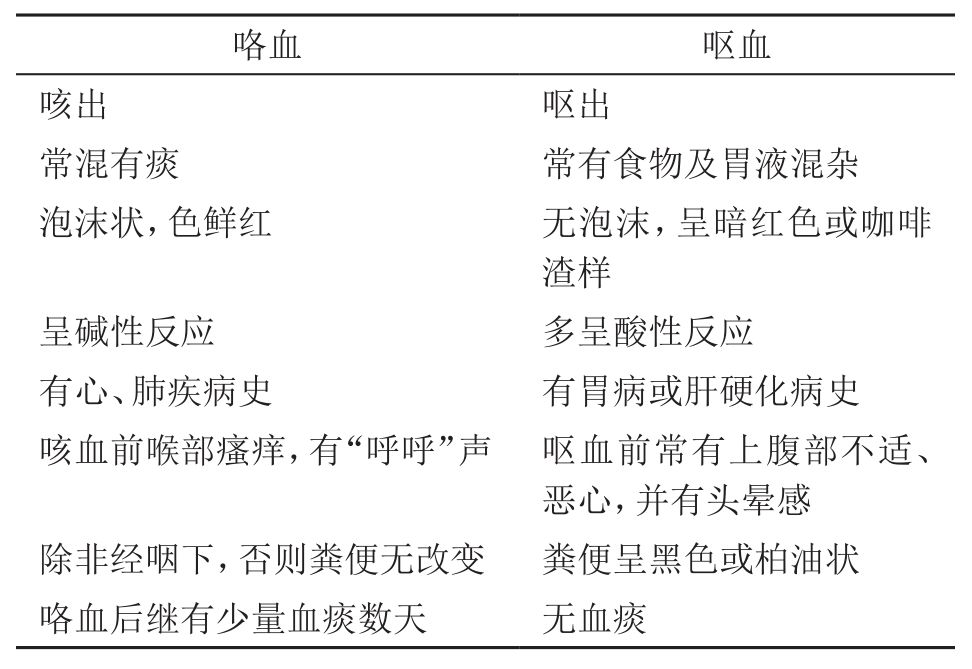
\includegraphics[width=3.22917in,height=2.21875in]{./images/Image00053.jpg}
\end{table}

当确认患者是上消化道出血后,需要迅速对下列问题作出判断,以便及时采取相应的处理。

\subsubsection{出血严重程度的估计和周围循环状态的判断}

对制定合理的治疗方案极为重要。

\paragraph{失血量的判断与临床分级}

上消化道出血病情严重度与失血量呈正相关。一般而言,粪便隐血试验阳性提示每日失血量在5ml以上;出现黑粪者,每日出血量在50~70ml以上;如短期内出血量在250~300ml,多可导致呕血。因呕血与黑便混有胃内容物与粪便,而部分血液贮留在胃肠道内未排出,故难以根据呕血或黑便量精确判断出血量。常根据临床综合指标判断失血量的多寡,对出血量判断通常分为:大量出血(急性循环衰竭,需输血纠正者。一般出血量在1000ml以上或血容量减少20\%以上)、显性出血(呕血或黑便,不伴循环衰竭)和隐性出血(粪隐血试验阳性)。临床可以根据血容量减少导致周围循环的改变(伴随症状、脉搏和血压、化验检查)来判断失血量,并根据患者年龄、有无伴发病、失血量等指标将上消化道出血严重程度分为轻、中、重度三级(表\ref{tab13-2})。

\paragraph{体位倾斜试验}

方法为先测平卧位时的血压(V\textsubscript{0}
)、脉搏(P\textsubscript{0}
),改为半卧位3分钟后,再测血压(V\textsubscript{1}
)、脉搏(P\textsubscript{1}
),符合下列条件之一者,提示失血量在1000ml以上。①V\textsubscript{0} −
V\textsubscript{1} >10mmHg;②P\textsubscript{1} − P\textsubscript{0} >
20次/分;③改半卧位后出现头晕、晕厥。必须在输液通路建立后才能进行,休克者禁作此试验。

\paragraph{休克指数}

为脉搏(次/分)与收缩压(mmHg)的比值(P/SBP),指数正常值约为0.58。指数为1.0,大约失血800~1200ml(占血容量20\%~30\%);指数大于1.0,失血量1200~2000ml(占血容量30\%~50\%)。

\paragraph{Hb、RBC和Hct的测定}

是估计失血量及决定输血量的重要参考指标。但在急性失血早期,由于血液浓缩及血液重新分布等代偿机制,上述指标可暂时无变化。一般出血3~4小时后,组织液渗入血管内补充血容量,患者可出现贫血,约24~72小时左右Hb稀释到最大限度。在连续测定中,三者迅速下降,表示继续出血,经输血纠正血容量后,与出血前比较,Hb每下降10g/L提示失血容量约400ml。

应指出的是,急性大出血严重程度的估计最有价值的指标是血容量减少所导致周围循环衰竭的临床表现,而周围循环衰竭又是急性大出血导致死亡的直接原因。因此,对急性消化道大出血患者,应将对周围循环状态的有关检查放在首位,并据此作出相应的紧急处理。血压和心率是关键指标,需进行动态观察,综合其他相关指标加以判断。如患者体位倾斜试验阳性,则提示血容量明显不足,是紧急输血的指征。如收缩压<
90mmHg,HR >
120次/分,伴有面色苍白,四肢湿冷,烦躁不安或神志不清则已进入休克状态,属严重大量出血(指3小时内需输血1500ml才能纠正其休克),需积极抢救。

\begin{table}[htbp]
\centering
\caption{上消化道出血病情严重程度分级}
\label{tab13-2}
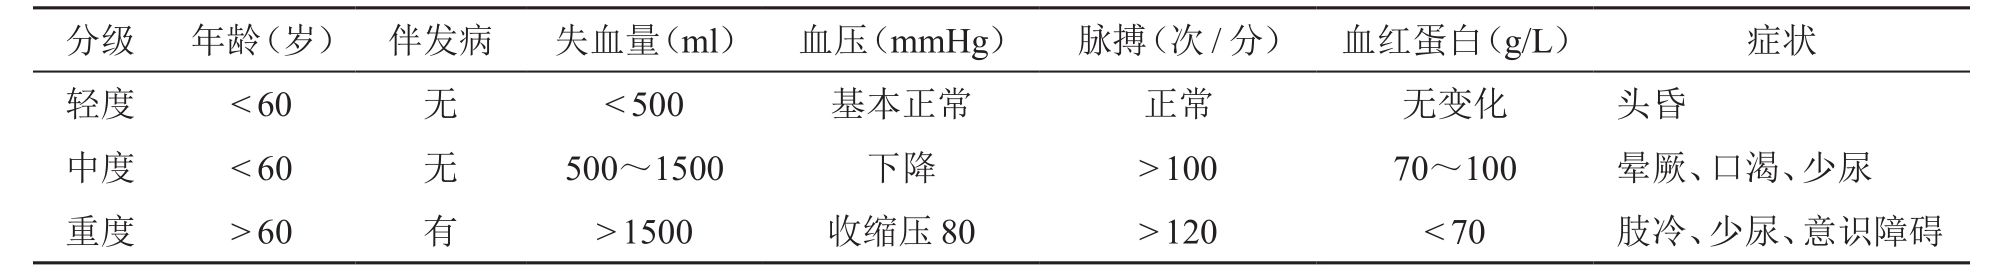
\includegraphics[width=6.65625in,height=0.91667in]{./images/Image00054.jpg}
\end{table}

\subsubsection{出血是否停止的判断}

临床上不能单凭Hb在下降或大便柏油样来判断出血是否停止或持续。因为一次出血后,Hb的下降有一定过程;而一次出血后柏油样大便持续天数受患者排便次数及出血量的影响。如每日排便1次,出血量在1000ml左右者,柏油样大便可持续1~3天,隐血试验阳性可达1周;若出血量在2000ml左右,柏油样大便可持续4~5天,隐血试验阳性达2周。应综合分析,特别是血压与脉搏的反复测定,直至恢复正常并趋稳定,尿量足(>
30ml/h),患者一般情况明显恢复者,方可认为已无活动性出血。有下列表现者,应认为有持续出血或再出血:①反复呕血或柏油样便次数及量增多,质稀薄,甚至排出暗红或鲜红色血便,伴肠鸣音活跃。②胃管抽出物有较多新鲜血。③周围循环衰竭的表现经积极补充血容量仍未见明显改善,或曾一度好转又很快恶化,中心静脉压仍有波动,稍稳定又再下降。④在补液量和排尿量足够的情况下,原无肾脏病变患者的BUN持续或再次升高。⑤Hb、RBC和Hct持续下降,血中网织红细胞持续增高。

肝硬化门静脉高压食管胃静脉曲张出血的防治共识(2008,杭州)关于EGVB继续出血或再出血的评估:①提示EGVB出血未控制的征象:72小时内出现以下表现之一者为继续出血。6小时内输血4个单位以上,生命体征不稳定。收缩压<
70mmHg,HR > 100次/分或心率增加> 20
次/分;间断呕血或便血,收缩压降低20mmHg以上或心率增加>
20次/分,继续输血才能维持Hb含量稳定;药物或内镜治疗后新鲜呕血,在没有输血的情况下,Hb含量下降30g/L以上。②提示EGVB再出血的征象:出现以下表现之一者为再出血。出血控制后再次有活动性出血的表现(呕血或便血;收缩压降低20mmHg以上或心率增加>
20
次/分;在没有输血的情况下,Hb含量下降30g/L以上)。早期再出血:出血控制后72小时~6周内出现活动性出血。迟发性再出血:出血控制6周后出现活动性出血。

\subsubsection{出血的病因诊断}

对上消化道大出血的患者,应首先纠正休克,然后尽快查找出血的部位与病因,以决定进一步的治疗措施和判断预后。一般通过询问病史、体检和必要的辅助检查,可明确出血的病因。

\paragraph{病史与体检}

详询病史和系统体检,仍是出血病因与部位诊断的基础。约50\%的患者可据此作出病因诊断。慢性、周期性、节律性上腹痛多提示出血来自消化性溃疡,特别是在出血前疼痛加剧,出血后减轻或缓解,更有助于消化性溃疡的诊断。有服用非甾体抗炎药等损伤胃黏膜的药物或应激状态者,可能为急性糜烂出血性胃炎。对中年以上的患者近期出现上腹痛,伴有厌食、消瘦者,应警惕胃癌的可能性。既往有病毒性肝炎、血吸虫病或酗酒病史,并有肝病与门静脉高压的临床表现,可能是食管胃底静脉曲张破裂出血。尚应注意既往有无类似出血史、诊治情况等。

\paragraph{急诊内镜检查}

急诊内镜检查是UGIB病因诊断中的首选方法。诊断正确率达80\%~94\%。急性上消化道出血的内镜检查有如下优点:①诊断正确率高:首先,内镜检查结合活检,既可明确出血部位,又可获得出血病变性质的诊断;其次,对一些上消化道钡餐检查不易发现的急性胃黏膜病变、贲门黏膜撕裂综合征、浅溃疡、胃黏膜毛细血管扩张症等,内镜可迅速作出诊断;第三,肝硬化合并上消化道出血病例,非静脉曲张破裂出血者占50\%左右,这仅能由内镜检查才能确诊。②提供预后的依据:如内镜下见溃疡基底喷血,溃疡基底血管、凝血块或红点等内镜征象可预示有再发出血的危险。③作为治疗手段:内镜诊断结合激光、高频电凝、喷洒止血剂以及给出血的曲张静脉内注射硬化剂等治疗性内镜的应用,使内镜检查不仅成为诊断工具,而且可作为止血治疗的方法。

\hypertarget{text00032.htmlux5cux23CHP1-13-1-4-4-2-1}{}
(1) NVUGIB的内镜检查:

①内镜检查能发现上消化道黏膜的病变,应尽早在出血后24~48小时内进行,并备好止血药物和器械。②内镜检查无食管胃底静脉曲张并在上消化道发现有出血病灶,NVUGIB诊断可确立。③内镜检查时根据溃疡基底特征,可用来判断病变是否稳定,凡基底有血凝块、血管显露等易于再出血。内镜检查时对出血灶病变应作Forrest分级(表\ref{tab13-3})。④应仔细检查贲门、胃底部、胃体垂直部、胃角小弯、十二指肠球部后壁及球后处,这些部位是易遗漏病变的区域。当检查至十二指肠球部未能发现出血病变者,应深插内镜至乳头部检查。发现有2个以上的病变,要判断哪个是出血性病灶。⑤有内镜检查禁忌证者不宜作此检查:如心率>
120次/分,收缩压< 90mmHg或较基础收缩压降低> 30mmHg、血红蛋白<
50g/L等,应先迅速纠正循环衰竭,血红蛋白上升至70g/L后再行检查。危重患者内镜检查时应进行血氧饱和度和心电、血压监护。

\begin{table}[htbp]
\centering
\caption{出血性消化性溃疡的 Forrest分级}
\label{tab13-3}
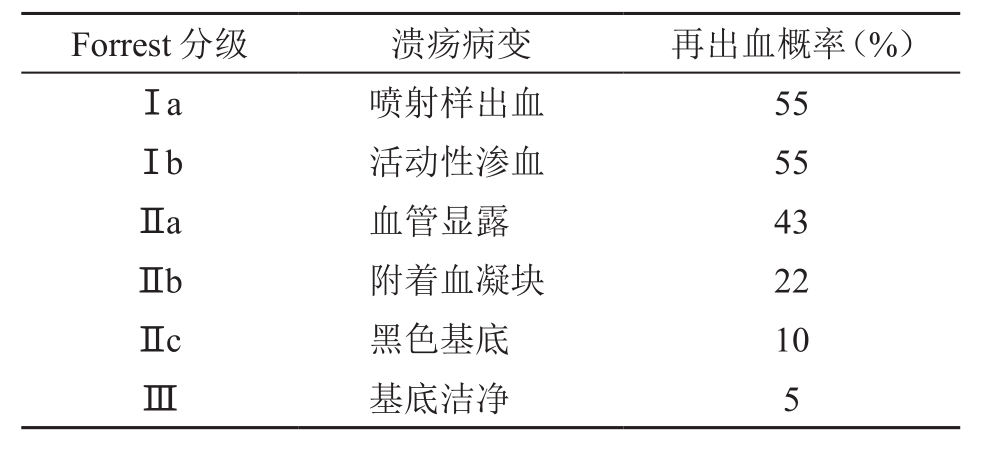
\includegraphics[width=3.26042in,height=1.5in]{./images/Image00055.jpg}
\end{table}

\hypertarget{text00032.htmlux5cux23CHP1-13-1-4-4-2-2}{}
(2) EGVB的内镜检查:

①内镜检查见有食管或胃曲张静脉出血,EGVB诊断即可成立;内镜检查时发现粗大曲张静脉和胃内血液而无其他可以识别的出血原因,EGVB诊断也可成立。②按食管静脉曲张形态及出血危险程度可将食管静脉曲张分轻、中、重3级。轻度(G\textsubscript{1}
):食管静脉曲张呈直线形或略有迂曲,无红色征(曲张静脉表面红斑、红色条纹和血疱)。中度(G\textsubscript{2}
):食管静脉曲张呈直线形或略有迂曲,有红色征或食管静脉曲张呈蛇形迂曲隆起但无红色征。重度(G\textsubscript{3}
):食管静脉曲张呈蛇形迂曲隆起且有红色征或食管静脉曲张呈串珠状、结节状或瘤状(不论是否有红色征)。③有内镜检查禁忌证者不宜作此检查(见前述)。

\hypertarget{text00032.htmlux5cux23CHP1-13-1-4-4-2-3}{}
(3) 内镜阴性患者的病因检查:

①仍有活动性出血的患者,应急诊行选择性腹腔动脉或肠系膜动脉造影,以明确出血部位和病因,必要时同时作栓塞止血治疗。②在出血停止,病情稳定后可作胃肠钡剂造影或放射性核素扫描(如\textsuperscript{99m}
锝标记患者的红细胞),但此检查特异性差。③对慢性隐性出血或少量出血者,可考虑作小肠镜检查。④对经各种检查仍未能明确诊断而出血不停者,病情紧急时可考虑剖腹探查,可在术中结合内镜检查,明确出血部位。

\paragraph{X线钡餐检查}

目前已多为胃镜检查所替代。消化道大出血患者,因休克不能站立和充分变换体位,胃内潴留大量血液或血块影响钡餐充盈和病变征象观察,不易显示某些浅表病变如胃炎、急性胃黏膜病变等,仅能发现病变而不能确定是否为出血病变等,还可干扰以后内镜检查和血管造影检查,以及在活动性出血时,过早进行此项检查有加重出血的危险等因素,使急诊X线钡餐检查的实用性大大受到限制。因此,上消化道钡餐检查仅适用于出血已停止、生命体征平稳的上消化道出血患者。但对经胃镜检查出血原因未明、疑病变在十二指肠降段以下小肠段,则有特殊诊断价值。对某些解剖部位的改变,如胃黏膜脱垂、食管裂孔疝的诊断却优于一般胃镜检查。一般宜在出血完全停止3天后谨慎进行。

\paragraph{血管造影}

对内镜检查无阳性发现或不适宜进行内镜检查者如有严重的心、肺并发症,且仍有活动性出血的患者可做选择性血管造影,对肠血管畸形、小肠平滑肌瘤等有很高的诊断价值,并可同时进行介入治疗。但忌用于严重动脉硬化、对碘剂过敏和老年患者。该检查的优点是:①灵敏性强:实验证明,出血量在0.5ml/min以上的消化道出血,在选择性血管造影连续摄影中即可见到造影剂从破裂血管外溢的X线征象。对慢性、隐源性活动性消化道出血是一种极有价值的诊断方法,阳性率一般为77\%~90\%。一般选择肠系膜上动脉及腹腔动脉造影已足够显示所要的范围。②具有精确的出血定位诊断价值:经出血相关区域血管注射造影剂,可精确显示出血部位和出血病变的供应动脉,为确定治疗提供了精确的解剖依据。③消化道内积血或血块不影响血管造影剂外溢的X线征象观察。④出血部位及其供应动脉显示后,立即经血管造影导管注射血管收缩剂或血管栓塞剂进行止血治疗。此外,门静脉造影(包括经脾穿刺门静脉造影、经肝穿刺门静脉造影以及经脐静脉插管门静脉造影等)除可以显示血管破裂部位、进行栓塞治疗外,还可以经导管测量门静脉压力诊断门脉高压症。

\paragraph{放射性核素扫描}

经内镜及X线检查阴性的病例,可做放射性核素扫描。方法是采用核素(如\textsuperscript{99m}
锝)标记患者的红细胞后,再从静脉注入患者体内,当有活动性出血,且出血速度达到0.1ml/min,核素便可显示出血部位。注射一次\textsuperscript{99m}
锝标记的红细胞,可以监视患者消化道出血达24小时。本法缺点为出血部位定位不够确切,也不能确定出血病变的性质。

\subsubsection{预后估计与危险性分级}

约80\%~85\%急性上消化道出血患者除支持疗法外,无需特殊治疗出血可在短期内自然停止。仅有15\%~20\%患者持续出血或反复出血,而主要是这类患者由于出血并发症而导致死亡。如何早期识别再出血及死亡危险性高的患者,并给予加强监护和积极治疗,便成为急性上消化道出血处理的重点。提示预后不良、危险性增高的主要因素有:①高龄患者(>
60岁);②有严重伴随病(心、肺、肝、肾功能不全,脑卒中等);③本次出血量大或短期内反复出血;④特殊病因和部位的出血(如食管胃底静脉曲张破裂出血);⑤消化性溃疡伴有内镜下活动性出血,或近期出血征象。此外,EGVB出血48小时内肝静脉压力梯度(HVPG)>
20mmHg是其可靠的预后不良预测因子。

Rockall评分系统(表\ref{tab13-4}\footnote{\textsuperscript{※} 收缩压> 100mmHg,心率<
100次/分;\textsuperscript{△} 收缩压> 100mmHg,心率>
100次/分;\textsuperscript{▲} 收缩压< 100mmHg,心率> 100次/分})仍是目前临床广泛使用的评分依据,该系统依据患者年龄、休克状况、伴发病、内镜诊断和内镜下出血征象5项指标,将UGIB患者分为高危、中危或低危三级,积分≥5分者为高危,3~4分为中危,0~2分为低危。在Rockall评分系统中,若仅根据年龄、休克表现及伴发病三个指标评判疾病危险度,谓之为临床Rockall评分系统,可适用于无条件获取急诊内镜资料的基层医院;若同时有急诊内镜资料参与评估,谓之为完全Rockall评分系统。如出血患者,61岁,收缩压为105mmHg,心率为110次/分,胃镜下可见一巨大溃疡,活检示胃腺癌,附血凝块,无伴发病。则该患者Rockall积分=年龄(1)+心动过速(1)+无伴发病(0)+胃癌(2)+近期出血征象(2)=
6分,为高危患者。

Blatchford评分系统(表\ref{tab13-5}\footnote{积分≥6分为中高危,< 6分为低危;1mmHg = 0.133kPa})包含了BUN、Hb等实验室检查信息,其价值逐渐得到认可。

\begin{table}[htbp]
\centering
\caption{急性 UGIB患者的Rockall再出血和死亡危险性评分系统}
\label{tab13-4}
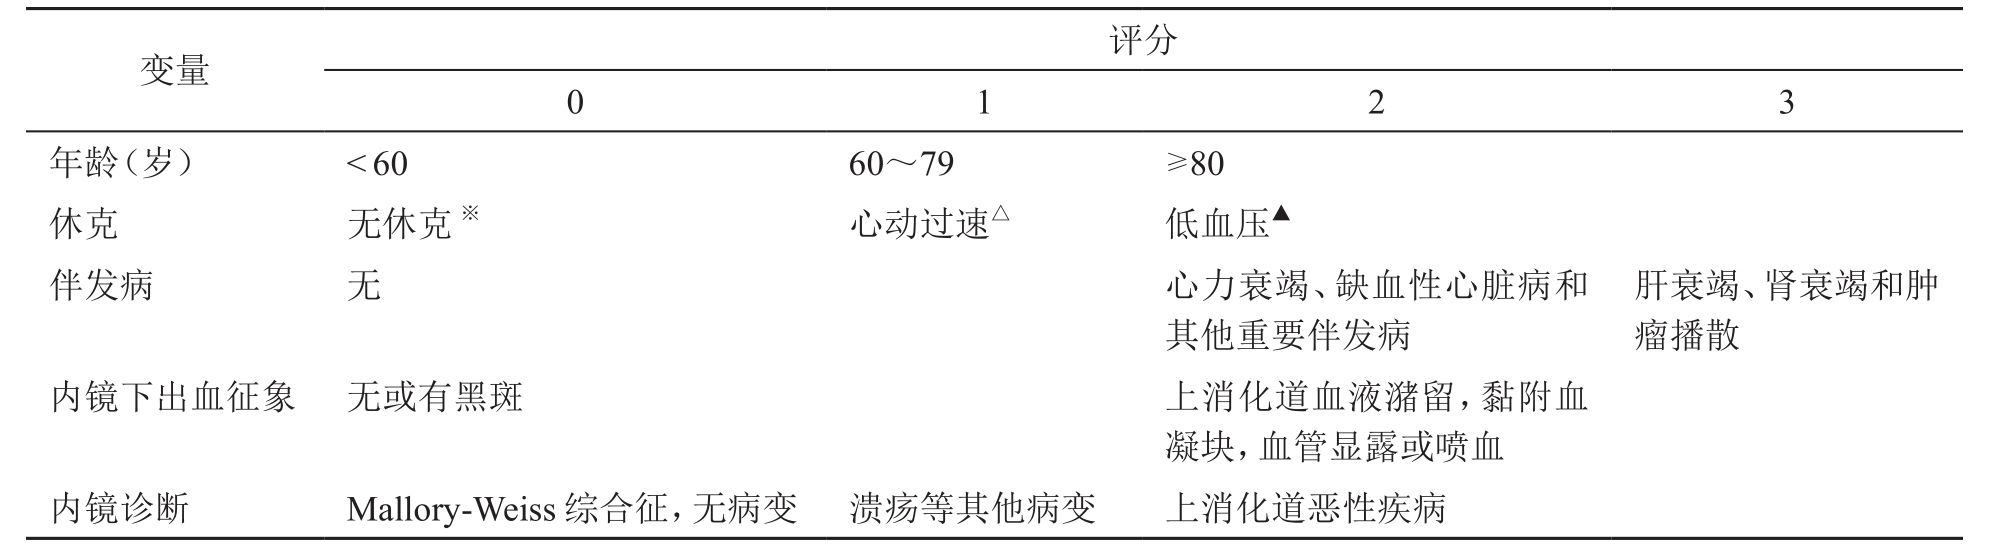
\includegraphics[width=6.67708in,height=1.83333in]{./images/Image00056.jpg}
\end{table}

\begin{table}[htbp]
\centering
\caption{急性上消化道出血患者的 Blatchford评分}
\label{tab13-5}
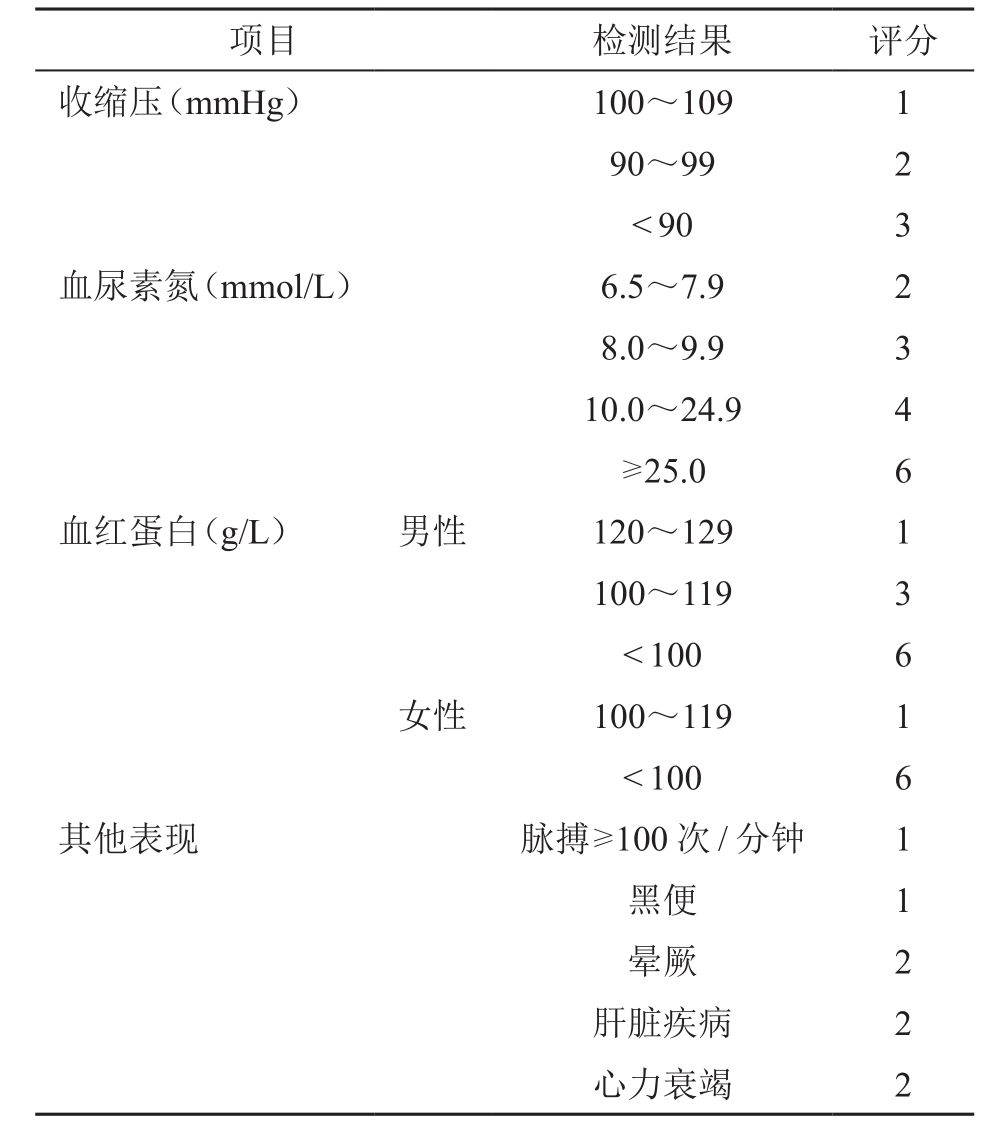
\includegraphics[width=3.32292in,height=3.75in]{./images/Image00057.jpg}
\end{table}

\subsection{处理原则}

及早补充血容量、防治继续出血和再出血及病因治疗。其中,抗休克、迅速补充血容量应放在一切医疗措施的首位。

关于UGIB诊治流程,中国医师协会急诊医师分会制定的《急性上消化道出血急诊诊治专家共识》将上消化道出血的急诊诊治过程分为三个阶段,分别是紧急治疗期、病因诊断期和加强治疗期。紧急治疗期:患者入院6~48小时,治疗目标是控制急性出血、维持患者生命体征平稳并针对患者病情做出初步诊断及评估,治疗手段以药物治疗为主(PPI、生长抑素和抗菌药物联合用药)。病因诊断期:入院48小时内,急性出血得到控制,患者血流动力学稳定的情况下,行急诊内镜检查以明确病因并进行相应的内镜下治疗。无法行内镜检查的患者,可根据情况进行经验性诊断、评估和治疗。加强治疗期:入院后3~7天,治疗目标是病因治疗,预防早期再出血的发生。病因明确后,可根据不同病因采取不同的治疗手段。临床推荐采用以药物联合内镜治疗为主的综合治疗方法。

\subsubsection{一般措施}

患者应取平卧位休息,吸氧,严密观察患者的神色、血压、脉搏、出血量和尿量;保持静脉通道通畅,必要时作静脉切开。保持呼吸道通畅,避免呕血时引起窒息。烦躁不安者可给予镇静剂,如地西泮(安定)10mg肌注,对肝病患者忌用巴比妥类药物。呕血者宜暂禁食,但少量出血者宜进流质(因为胃内空虚产生饥饿的不正常的胃收缩不利于止血),活动性出血停止后可逐渐改变饮食的质与量。推荐对活动性出血或大出血患者宜常规放置胃管,其意义有:①可以观察出血情况,并可用冰盐水洗胃止血;②抽取胃内容物,减轻胃扩张,改善胃黏膜的循环,抽出积存在胃内的血液,能减轻日后吸收热和氮质血症,降低胃内酸度,防止凝血块被消化,有利于止血;③可通过胃管及时用药治疗;④预防吸入性肺炎;⑤鼻饲营养液。意识障碍和排尿困难者需留置尿管,危重大出血者必要时进行中心静脉压测定,老年患者常需心电、血氧饱和度、呼吸监护。

\subsubsection{迅速补充血容量}

迅速补充血容量是处理上消化道大出血的首要措施。立即查血型和配血,尽快建立有效的静脉输液通道,尽快补充血容量。在配血过程中,可先输平衡液或葡萄糖盐水。失血量较大(如减少20\%血容量以上)时,可输入血浆等胶体扩容剂。改善急性失血性周围循环衰竭的关键是要输血,一般输浓缩红细胞,严重活动性大出血考虑输全血。下列情况为紧急输血指征:①收缩压<
90mmHg(EGVB时< 80mmHg),或较基础收缩压降低幅度> 30mmHg;②Hb <
50~70g/L(EGVB时Hb < 50g/L),Hct < 25\%;③心率增快(>
120次/分)。输血量依失血量而定,原则上输血量应接近出血量。输血注意事项:①输血开始时,速度应加快,以尽快把收缩压升高至80~90mmHg水平,待血压稳定、病情改善后则减慢输血、输液速度,避免依赖升压药来维持血压。②避免输血、输液过多、过快,招致急性肺水肿,尤其是对有心、肺、肾疾患及老年患者。③防止枸橼酸中毒,一般每输血600~900ml可从静脉注入10\%葡萄糖酸钙10ml,以防低钙。④大量输注库存血时易引起高钾血症,应注意给予高渗葡萄糖,必要时加用适量胰岛素。⑤对肝硬化门脉高压静脉曲张破裂出血时,应输新鲜全血,除恢复血容量外,尚因其含有多种凝血因子和血小板成分,对止血有益;还可避免输库存血(含氨多)过多诱发肝性脑病。另外,输入的血约为失血量的2/3或3/4,以避免门静脉压力增高致再出血的危险。对于EGVB,以维持血流动力学稳定并使Hb维持在80g/L以上;过度输血或输液可能导致继续或重新出血;避免仅用氯化钠溶液补足液体,以免加重或加速腹水或其他血管外液体的蓄积;必要时应及时补充凝血因子、凝血酶原复合物等;血小板<
50 × 10\textsuperscript{9}
/L者,可输注血小板。对于急性大量出血者,应尽可能施行中心静脉导管置管和中心静脉压监测,以指导液体复苏。在补足液体的前提下,如血压仍不稳定,可以适当地选用血管活性药物(如多巴胺)以改善重要脏器的血液灌注。血容量充足的指征:①神志清楚或好转,无明显脱水貌;②收缩压90~120mmHg;③脉搏<
100次/分;④尿量> 40ml/h,血钠< 140mmol/L。

\subsubsection{非静脉曲张性上消化道出血(nonvariceal UGIB,NVUGIB)的止血措施}

NVUGIB是指除食管胃底静脉曲张破裂出血以外的其他病因引起的上消化道出血。包括消化性溃疡、急性糜烂出血性胃炎、胃泌素瘤、食管裂孔疝等所致的出血。止血措施主要有:

\paragraph{内镜下止血}

起效迅速、疗效确切,应作为首选。可根据医院的设备和病变的性质选用,常用方法有:

\hypertarget{text00032.htmlux5cux23CHP1-13-1-5-3-1-1}{}
(1) 对出血灶喷洒止血药物:

内镜下直接对出血灶喷洒止血药物,对局部渗血疗效较好,对动脉性出血疗效较差。常用的药物有去甲肾上腺素溶液、孟氏液、注射用血凝酶、凝血酶等。

\hypertarget{text00032.htmlux5cux23CHP1-13-1-5-3-1-2}{}
(2) 局部注射法:

当内镜检查发现喷射性出血或血管显露时,可用局部注射法止血。常用的注射剂有肾上腺素溶液、凝血酶、无水酒精、高渗盐水等。其方法是在出血血管周围1~2mm处选3~4点,每点注入0.1~0.3ml。本法安全、有效,且可反复应用。

\hypertarget{text00032.htmlux5cux23CHP1-13-1-5-3-1-3}{}
(3) 激光照射法:

可供止血的激光有氩激光(Argon)和镱-铝-石榴石激光(Nd-YAG)两种。后者功率大,止血效果好。止血机制是由于光凝作用,使照射局部组织蛋白凝固,小血管内血栓形成。止血成功率在80\%~90\%。其并发症有胃肠穿孔、出血及胃肠胀气等。

\hypertarget{text00032.htmlux5cux23CHP1-13-1-5-3-1-4}{}
(4) 微波凝固法:

将微波经内镜导入出血部位,使产生热凝固,达到止血目的。其优点是,操作简便,并可将微波针状电极直接插入组织内治疗,插入组织的深度易控制,因而止血目标确切,安全性大。

\hypertarget{text00032.htmlux5cux23CHP1-13-1-5-3-1-5}{}
(5) 高频电凝止血法:

应用高频电流的热效应,使局部组织蛋白变性达到止血,迅速止血率达87\%~96\%。主要用于血管显露性出血及有直接出血征象的出血性病变。方法是用凝固电流在出血灶周围电凝,使黏膜下层或肌层的血管凝缩,最后电凝出血血管。有出血、溃疡、穿孔等并发症。近年来为了提高电凝止血的安全性和止血效果,研制出各种形状的及带喷水孔的单极电凝头、双极电凝头及四头双极电凝探头。

\hypertarget{text00032.htmlux5cux23CHP1-13-1-5-3-1-6}{}
(6) 热探头凝固法:

是利用热探头的高温(150℃)接触出血灶,使其组织蛋白质凝固而达到止血。此法疗效确切、安全、简单。

\hypertarget{text00032.htmlux5cux23CHP1-13-1-5-3-1-7}{}
(7) 放置止血夹法:

内镜直视下放置止血夹子,把出血的血管夹住止血,伤口愈合后此金属夹子自行脱落随粪便排出体外,此法止血既安全又有效。适用于消化性溃疡、急性胃黏膜病变的出血治疗,尤其在小动脉出血时用该法甚佳。

\paragraph{制酸药物的应用}

胃酸在上消化道出血中起重要作用,抑制胃酸分泌及中和胃酸可达到止血的效果。制酸药止血的关键是使胃内pH维持在>
6,这样,既可促进血小板聚集和纤维蛋白凝块的形成,避免血凝块过早溶解,有利于止血和预防再出血,又可治疗消化性溃疡等病变。尤适用于消化性溃疡、急性胃黏膜病变、胃泌素瘤、食管裂孔疝等所致的出血。常用制剂有:

\hypertarget{text00032.htmlux5cux23CHP1-13-1-5-3-2-1}{}
(1) 中和胃酸药:

将胃内容物抽尽,用氢氧化铝凝胶60ml经胃管注入,15分钟后测胃液pH,若<
6,再注入60ml,以后每小时测pH1次,使其值维持在> 6。

\hypertarget{text00032.htmlux5cux23CHP1-13-1-5-3-2-2}{}
(2) H\textsubscript{2} 受体阻滞剂(H\textsubscript{2} RA):

目前临床上常用的有:第一代的西咪替丁(cimetidine,甲氰咪胍)、第二代的雷尼替丁(ranitidine)和第三代的法莫替丁(famotidine)。由于后两者不仅抗酸作用强(雷尼替丁比西咪替丁强5~8倍,法莫替丁比西咪替丁强30~100倍),作用时间更持久,且毒副作用相对较轻,应作为首选。可用雷尼替丁50mg缓慢静脉注射,每6~12小时1次,或用150~300mg加入液体中持续静滴;法莫替丁20mg溶入生理盐水或葡萄糖液20ml中,缓慢静脉注射,每日2次。

\hypertarget{text00032.htmlux5cux23CHP1-13-1-5-3-2-3}{}
(3) 质子泵抑制剂(proton pump inhibition,PPI):

可抑制胃壁细胞的H\textsuperscript{+} -K\textsuperscript{+}
-ATP酶,从而抑制胃酸的分泌。其抑制胃酸作用远强于H\textsubscript{2}
RA,几乎完全抑制酸分泌,持续用药无耐受性,且作用持久、递增,3~5天达稳态,胃内pH维持平稳。大剂量PPI可减少高危患者再出血率,且总费用降低,是治疗NVUGIB的首选止血药物。加拿大NVUGIB共识会议推荐内镜止血成功后应用PPI,在待行内镜检查时也应给予大剂量PPI,并认为H\textsubscript{2}
RA不能减少再出血率及病死率,不提倡用H\textsubscript{2}
RA止血。PPI常用制剂有:奥美拉唑(omeprazole,又名洛赛克,Losec)、泮托拉唑(pantoprazole)和兰索拉唑(lansoprazole)等。PPI给药方法及剂量:高危患者应静脉给药,如奥美拉唑静脉推注80mg后,以8mg/h输注72小时;如低危患者可口服给药,如奥美拉唑20mg,每6小时一次,持续5天。

\paragraph{奥曲肽(octreotide)}

商品名善得定(Sandostatin),是人工合成的生长抑素类似品。能抑制胃酸、胃蛋白酶和胃泌素分泌,促进胃黏膜生长,能选择性引起内脏循环血流量减少和门脉压下降。用法:100μg皮下注射,每日2~4次。

\paragraph{去甲肾上腺素}

可使胃肠黏膜出血区域的小动脉强烈收缩,减少局部血流量,并能减少胃酸分泌,有类似迷走神经切断的作用;同时因可降低门脉压,故亦用于食管静脉曲张破裂出血。用法有二:①口服或胃管内灌入:用去甲肾上腺素8mg加入冷生理盐水100~200ml中为1次量,口服或由胃管内灌入,每0.5小时1次,共2~4次;若有效,可再改为1小时1次,共4~6小时,以后每2小时1次共4~6小时。若无效,则不用。②腹腔灌注:以细长穿刺针作腹腔穿刺,注入含去甲肾上腺素8mg的生理盐水100ml,然后来回转动患者腹部,出血可迅速停止。本法适用于有腹水者,以免注入组织内引起缺血性坏死。

\paragraph{注射用血凝酶(立止血,reptilase)}

是酸性止血剂,含有如凝血激酶和凝血酶样物质,可直接作用于内、外源性凝血系统形成凝血活酶,促进凝血酶的形成而起到凝血作用。用法:首次静注与肌注各1kU,继而每日肌注1kU。无明显毒副作用。

\paragraph{凝血酶(thrombin)}

本品是从猪血提取、精制而得的凝血酶无菌制剂。能直接作用于出血部位的纤维蛋白原,使其转变为纤维蛋白,促使血液凝固、填塞出血点而止血;尚有促进上皮细胞的有丝分裂而加速创伤愈合的作用。其特点是局部止血迅速,疗效显著,无明显不良反应,但出现过敏反应时,应立即停用。首次剂量宜大(8000U~2万U),溶入50~100ml生理盐水或牛奶、豆汁内口服或胃管内注入,每2~6小时1次,应用次数视病情而定。凝血酶遇热或在酸性环境中均易失去活性,故溶液温度不要超过37℃,同时给予抑酸药物(如H\textsubscript{2}
受体阻滞剂、质子泵抑制剂)以便得以发挥最大作用。本品切忌血管内或肌内注射。

\paragraph{其他止血药物}

以下止血药物对NVUGIB的确切效果未能证实,不作为一线药物使用。应避免滥用止血药。可酌情选用的有:①维生素K:能促进凝血酶原及凝血因子Ⅷ、Ⅵ、Ⅳ、Ⅹ在肝内合成。可用维生素K\textsubscript{1}
10mg肌注,每日2次;或维生素K\textsubscript{4}
口服4mg,每日3次;②肾上腺色腙(安络血):可增强受损毛细血管的修复能力,从而达到止血目的。10mg肌注,每天2次;或5~10mg口服,每天3~4次。③酚磺乙胺(止血敏):有增强血小板的作用。0.5~1.0g口服,每天3次;或0.5g肌注或静注。④氨甲苯酸(止血芳酸)、氨基己酸:能抑制纤溶酶原的激活因子和抑制纤维蛋白的溶解。⑤中药:云南白药、三七粉、白及粉、血余炭等均有防腐生肌、凉血止血的作用,中成药如止血散(白及、煅瓦楞、三七、甘草)、止血粉(白及、蒲黄、地榆、甘草)、止血汤(仙鹤草、地榆炭、白及、生槐花)等可酌情辨证选用。

\paragraph{选择性血管造影及栓塞治疗}

选择性胃左动脉、胃十二指肠动脉、脾动脉或胰十二指肠动脉血管造影,针对造影剂外溢或病变部位经血管导管滴注血管升压素或去甲肾上腺素,导致小动脉和毛细血管收缩,使出血停止。无效者可用明胶海绵栓塞。

\paragraph{手术治疗}

诊断明确但药物和介入治疗无效者,诊断不明确、但无禁忌证者,可考虑手术,结合术中内镜止血治疗。约10\%的胃十二指肠溃疡大出血患者需急症手术止血,手术指征为:①出血速度快,短期内发生休克,或较短时间内(6~8小时)需要输入较大量血液(>
800ml)方能维持血压和Hct者;②年龄在60岁以上伴动脉硬化症者自行止血机会较小,对再出血耐受性差,应及早手术;③近期发生过类似的大出血或合并穿孔或幽门梗阻;④正在进行药物治疗的胃十二指肠溃疡患者发生大出血,表明溃疡侵蚀性大,非手术治疗难以止血;⑤内镜检查发现动脉搏动性出血,或溃疡底部血管显露再出血危险很大。急诊手术应争取在出血48小时内进行,胃溃疡较十二指肠溃疡再出血概率高3倍,应争取及早手术。

\paragraph{原发病的治疗}

对出血的病因比较明确者,如幽门螺杆菌阳性的消化性溃疡患者,应予抗幽门螺杆菌治疗及抗溃疡治疗。需要长期服用非甾体抗炎药者一般推荐同时服用PPI或黏膜保护剂。

非静脉曲张性上消化道出血诊治流程见图\ref{fig13-1}。

\subsubsection{食管胃静脉曲张出血的止血治疗}

肝硬化门脉高压症患者发生上消化道出血,并不全是由食管胃底静脉曲张破裂所致,而是多种因素共同作用的结果。因此,它的治疗仍应以上述治疗措施为基础。EGVB活动性出血的止血措施主要有内镜治疗、血管活性药物、经颈静脉肝内门体分流术(transjugular
intrahepatic portosystemic
shunt,TIPS)、外科手术和双气囊堵塞压迫等。其作用机制、运用方法及注意事项等有关内容,详见本书第116章第1节“肝硬化并上消化道出血”部分。

\subsubsection{预后}

据临床资料统计,约80\%~85\%急性上消化道大量出血的患者除支持疗法外,无需特殊治疗,出血可在短期内自然停止。仅有15\%~20\%患者持续出血或反复出血,常因出血并发症而导致死亡。如何早期识别再出血及死亡危险性高的患者,并予加强监护和积极治疗,便成为急性上消化道大量出血处理的重点。提示预后不良危险性增高的主要因素有:①高龄患者(>
60岁);②有严重伴随病(心、肺、肝、肾功能不全、脑卒中等);③本次出血量大或短期内反复出血;④特殊病因和部位的出血(如食管胃底静脉曲张破裂出血);⑤消化性溃疡伴有内镜下活动性出血,或近期出血征象。

\begin{figure}[!htbp]
 \centering
 \includegraphics[width=4.23958in,height=3.55208in]{./images/Image00058.jpg}
 \captionsetup{justification=centering}
 \caption{急性非静脉曲张性上消化道出血诊治流程}
 \label{fig13-1}
  \end{figure} 

PPIs:质子泵抑制剂;H\textsubscript{2} RA:H\textsubscript{2} 受体拮抗剂

\protect\hypertarget{text00033.html}{}{}

\section{下消化道出血}

下消化道出血(lower gastrointestinal
hemorrhage)是指屈氏韧带以下的小肠或大肠出血。依其出血量大小、速度和快慢等可分为三类:①慢性隐性出血:肉眼不能观察到便血,仅有大便隐血试验阳性,常以不明原因贫血就诊或普查时发现。②慢性少量显性出血(亚急性出血):表现为间歇性或持续性肉眼可见的少量显性便血,可呈鲜红色、果酱样或柏油样黑粪,无循环衰竭表现。③急性大量出血:短期内排出大量鲜红或暗红色血便,伴血压下降等休克症状,常需输血治疗者。多数下消化道出血相对缓慢,或呈间歇型,约80\%的出血能自行停止。在治疗上除了止血、补充血容量以外,寻找下消化道出血部位、疾病性质进行原发病病因治疗最为重要。

下消化道范围广,出血病因繁多,分类各异。如按病变部位可分为:①小肠疾病:小肠肿瘤、黑色素-胃肠息肉综合征、克罗恩病(Crohn病)、小肠憩室与Meckel憩室、肠套叠、小肠血管畸形、急性出血性坏死性肠炎、缺血性小肠炎和肠结核等。②大肠疾病:溃疡性结肠炎、结肠息肉、结肠憩室、菌痢、阿米巴痢疾、结肠癌、克罗恩病、缺血性结肠炎、结肠子宫内膜异位症、结肠结核及肠套叠、结肠血管畸形等。③直肠疾病:直肠溃疡、非特异性炎症、肿瘤、息肉、放射性直肠炎和腹盆腔邻近脏器恶性肿瘤或脓肿侵及直肠等。④肛管疾病:痔、肛裂、肛瘘。此外,还有全身性疾病累及肠道。国内资料引起下消化道出血的最常见病因为大肠癌和大肠息肉,其次为肠道炎症性疾病(其中肠伤寒、肠结核、溃疡性结肠炎、克罗恩病和坏死性小肠炎有时可发生大量出血)和血管病变,憩室引起的出血少见。但在西方国家,血管病变和消化道憩室是下消化道出血最常见病因,其次为结肠肿瘤和炎症性肠病。

\subsection{诊断思路}

\paragraph{下消化道出血的确立}

首先要排除口腔、鼻咽、喉、气管、支气管、肺等部位的出血被吞咽后由肛门排出的可能性,还要与下列情况区别:①口服某些中草药、兽炭、铁剂、铋剂时,大便可呈暗褐色或黑色,但隐血试验阴性;②食用过多的肉类、猪肝、动物血后大便可变暗褐色,隐血试验呈阳性,但素食后即转呈阴性;③口服酚酞制剂,大便有时呈鲜红色,不注意时易误诊为大量便血。

排除了上述因素后,要确定是否为下消化道出血,大便的色泽和量是重要的线索,通常大便呈鲜红色或暗红色者,即可确诊。但如为暗红色大量血便或仅表现为黑便或大便隐血阳性时,则应与上消化道出血鉴别。此时应常规行胃十二指肠镜检查,若未发现病变,大致可除外上消化道出血。

下述几点有助于下消化道出血的诊断:①病史中多伴有下腹痛或腹部有包块,排便异常伴便血史,出血前常有中下腹不适、下坠或便意。②大便常为鲜红、暗红、果酱样,少数为黑便,无呕血。③下消化道出血时胃管内无咖啡色的液体和暗红色的血液被抽出。④来自高位小肠的出血可能有血BUN升高,而结肠出血常不升高;上消化道出血时血BUN升高较下消化道出血时明显。⑤结直肠出血,常表现为鲜血便或是暗红的血便,血与大便相混,可有便后滴血,亦可表现为脓血便。⑥小肠出血常为暗红果酱样便,亦可为黑便,偶有血水样便。⑦大肠出血常伴有下腹痛、腹泻、里急后重等症状,而小肠出血常表现为脐周疼痛。

\paragraph{估计出血速度和出血量}

下消化道出血确定后,估计出血速度和出血量甚为重要。判断患者出血速度和出血量的最终标准取决于为恢复和维持血容量所需的输血量和速度。在此之前,则可根据有无循环障碍及其程度、Hct和Hb变化作出初步估计。

\paragraph{确定是否由全身性疾病所致下消化道出血}

全身性疾病所致的下消化道出血有相应疾病的全身表现。血液系疾病、血管疾病、肝脏疾病和某些中毒性疾病常伴有凝血与止血功能障碍,有凝血因子缺乏、血小板质或量改变、血管脆性增加、血管收缩障碍的实验室发现。相反,多数传染性疾病及中毒性疾病下消化道出血的主要原因是肠黏膜、黏膜下血管受损的后果。血液检查、骨髓检查、凝血机制检查等有助于诊断。

\paragraph{出血部位的判断}

下消化道出血最常见的部位是乙状结肠,占50\%左右。其他部位出血频率依次为直肠、降结肠、横结肠、升结肠、盲肠、小肠。根据出血类型常可对出血部位作出初步判断:仅大便隐血阳性者,若排除了上消化道出血,则多为右侧结肠和小肠出血;少量显性出血,则主要是结肠、直肠出血;鲜红或暗红色血便,以左半结肠和直肠为主;果酱色或咖啡色血便则多为右半结肠出血。虽右半结肠和小肠出血的发生率较低,但较易发生急性大出血。上位结肠出血时,血与大便常混杂;乙状结肠和直肠出血时,常有新鲜血液附着于成形大便的表面。血在大便后滴下,与粪便不相混杂者,虽多见于内痔、肛裂,但也可见于直肠息肉和直肠癌,应予以注意。

\paragraph{出血病因的诊断}

病史与体检是出血病因诊断中最重要的基础工作。

\hypertarget{text00033.htmlux5cux23CHP1-13-2-1-5-1}{}
(1) 既往史:

①反复小量显性出血史,提示痔、息肉、憩室等。②大便习惯改变或大便变细有切迹,应警惕结肠、直肠肿瘤。③反复血性腹泻史提示炎症性肠病可能。④曾患疾病与用药:曾患肺结核者应考虑肠结核;动脉硬化、心律失常、口服避孕药者应考虑缺血性结肠炎;风湿性疾病、白血病、出血性疾病、尿毒症、急性胰腺炎等病程中发生出血,多由于原发病引起的肠道病变;应用抗生素过程中出血应考虑假膜性肠炎、出血性结肠炎;便血前数月或数年曾接受腹部放射治疗者应考虑放射性结肠炎。

\hypertarget{text00033.htmlux5cux23CHP1-13-2-1-5-2}{}
(2) 便血特点与伴随症状:

①脓血黏液便伴里急后重或坠胀感,大便次数增多,应考虑痢疾和直肠癌可能。②中小量出血,色较红而呈间断性附于大便表面,要注意息肉出血之可能。③便血伴剧烈腹痛者,尤其是老年人心血管病患者,应警惕肠系膜血管栓塞;便血伴发热应考虑感染性肠炎、炎症性肠病、肠结核、肠伤寒、出血性坏死性肠炎、血液系疾病(白血病、恶性组织细胞病、恶性淋巴瘤等)等;便血伴腹块或不全性肠梗阻应考虑肿瘤、肠结核、Crohn病、肠套叠等;便血伴腹壁瘘管(或内瘘管),见于Crohn病、肠结核、癌、放线菌病。

\hypertarget{text00033.htmlux5cux23CHP1-13-2-1-5-3}{}
(3) 年龄与病因:

下消化道出血的病因与年龄有关:①婴儿和儿童:以Meckel憩室最多见,幼年性息肉次之,其他有炎症性肠病、肠套叠等。②青少年和成年人:在青少年时期,Meckel憩室依然是最常见病因,其次是炎症性肠病和息肉;随年龄增长癌肿比例显著增高。③老年人:以癌肿、息肉多见,其次为慢性结肠炎症、结肠血管扩张、结肠憩室等。

\hypertarget{text00033.htmlux5cux23CHP1-13-2-1-5-4}{}
(4) 出血部位与病因:

①直肠、乙状结肠:以息肉、癌、溃疡性结肠炎、单纯性溃疡、菌痢、阿米巴肠炎、放射性肠炎多见;②结肠脾曲、降结肠、乙状结肠:除息肉、癌外,易发生缺血性结肠炎;③右侧结肠:憩室、血管畸形、肠结核、Crohn病;④回盲部(回肠末段至升结肠始段):除癌、息肉外,类癌、Crohn病、单纯性溃疡、肠结核、鞭虫病、阿米巴肠炎、肠套叠、Meckel憩室、肠伤寒、沙门菌肠炎等。

\hypertarget{text00033.htmlux5cux23CHP1-13-2-1-5-5}{}
(5) 肛门视诊和直肠指检:

下消化道出血病因诊断的第一步,应采用简便易行的肛门视诊和直肠指诊,以发现或排除痔、肛裂,以及大部分直肠癌和息肉等常见的出血病因。

\hypertarget{text00033.htmlux5cux23CHP1-13-2-1-5-6}{}
(6) 内镜检查:

结肠镜检查是诊断大肠和回肠末端病变的首选检查方法。宜尽量在出血停止后近期或出血间歇期进行。对于出血灶的诊断,以窥视下直接见到活动性渗血最可靠。

\hypertarget{text00033.htmlux5cux23CHP1-13-2-1-5-7}{}
(7) X线钡剂造影检查:

一般要求在大出血停止至少3天后进行。主张双重气钡造影。其优点是基层医院已普及,患者易接受。缺点是对较平坦病变、广泛而较轻炎症性病变易漏诊,有时无法确定病变性质。对X线钡剂灌肠检查阴性的下消化道出血患者需进行结肠镜检查,已作结肠镜全结肠检查患者则不强调本项检查。

\hypertarget{text00033.htmlux5cux23CHP1-13-2-1-5-8}{}
(8) 胶囊内镜或双气囊小肠镜检查:

适用于常规内镜检查和X线钡剂造影不能确定出血来源的不明原因出血,出血活动期和静止期均可进行,可视病情和医疗条件选用。

\hypertarget{text00033.htmlux5cux23CHP1-13-2-1-5-9}{}
(9) 放射性核素扫描或选择性腹腔动脉造影:

必须在活动性出血时进行。主要用于急诊结肠镜检查不能确定出血来源的不明原因出血。放射性核素扫描检查的特点是简便敏感,出血量约0.1ml/min时即有阳性显示;缺点是对出血不能准确定位。常用本法初步确定出血部位,为进一步作血管造影提供线索。此外,利用\textsuperscript{99m}
Tc腹部扫描可用于诊断有胃黏膜异位的先天性病变,如Meckel憩室、肠重复畸形等。对持续大出血患者经上述检查不能明确出血灶时,应及时作选择性肠系膜上动脉造影,因肠系膜上动脉支配全部小肠和右侧结肠。约50\%~80\%的憩室出血和全部血管畸形出血均发生于右侧结肠。如肠系膜上动脉造影阴性,应再作肠系膜下动脉和腹腔动脉造影。血管造影可显示低至0.5ml/min的出血,此外还可显示肿瘤血管和血管畸形。成功的血管造影约于2/3的病例可显示肠出血来源。

\hypertarget{text00033.htmlux5cux23CHP1-13-2-1-5-10}{}
(10) 手术探查:

如上述检查仍不能明确出血灶,持续大出血危及患者生命,必须手术探查。术中内镜是明确诊断不明原因消化道出血,尤其是小肠出血的可靠方法。

不明原因消化道出血(obscure gastrointestinal bleeding,
OGIB)是指常规内镜检查(胃镜和结肠镜)不能确定出血来源的持续或反复消化道出血,多为小肠出血(如小肠的肿瘤、Meckel憩室和血管病变等),是消化道出血诊断的难点。OGIB的诊断步骤:在出血停止期,先行小肠钡剂检查;在出血活动期,应及时作放射性核素扫描或选择性腹腔动脉造影;若上述检查结果阴性则选择胶囊内镜或及双气囊小肠镜检查;出血不止危及患者生命者行手术探查,探查时可辅以术中内镜检查。

\subsection{处理原则}

下消化道出血主要是病因治疗,大出血时应积极抢救。

\paragraph{一般措施}

一般急救措施与补充血容量同上消化道出血一样。一般措施包括应用注射用血凝酶、静滴血管加压素、生长抑素、肾上腺色腙(安络血)、酚磺乙胺等药物。

\paragraph{局部止血措施}

对结肠出血,可给予冰盐水去甲肾上腺素液(去甲肾上腺素8mg加入100~200ml生理盐水中)、孟氏液、凝血酶等进行灌肠。

\paragraph{内镜下止血措施}

包括内镜下向出血病灶喷洒止血药物、高频电凝止血、激光止血、息肉电凝止血、黏膜和黏膜下注射硬化剂等措施止血。

\paragraph{放射性介入治疗}

在做选择性动脉造影时,若发现造影剂有渗出,即可通过导管给予血管加压素滴注,0.1~0.4U/min。对结肠出血不能自发地停止或血管加压素输注无效的病例,可施行栓塞治疗。在荧光透视下作超选择性插管,将管端插入出血灶近端几厘米处,注入明胶海绵碎片或自体凝血块,可将出血动脉栓塞、制止出血。

\paragraph{手术治疗}

经内科保守治疗仍出血不止危及生命,无论出血病变是否确诊,均是紧急手术的指征。此外,对下列情况可行手术治疗:①对Meckel憩室、肠重复畸形、恶性肿瘤、先天性动静脉畸形(包括结肠血管扩张)等皆可手术切除。②息肉病、家族性息肉病或有高度癌变倾向的息肉可手术切除。但一般息肉可经纤维结肠镜电凝切除。③溃疡性结肠炎引起的大出血是次全或全结肠切除的手术指征;Crohn病时如病变局限也可作局限性肠切除。

下消化道出血的处理程序如图\ref{fig13-2}。

\protect\hypertarget{text00034.html}{}{}

\section{不明原因消化道出血}

不明原因消化道出血(obscure gastrointestinal
bleeding,OGIB)是指常规的消化道内镜(包括检查食管至十二指肠降段的上消化道内镜与肛直肠至回盲瓣的结肠镜检查)和常规钡餐检查不能明确病因的持续或反复发作的出血。可分为不明原因的隐性出血和不明原因的显性出血。前者表现为反复发作的缺铁性贫血和大便隐血阳性,而后者则表现为黑便、血便等肉眼可见的出血。OGIB占消化道出血的3\%~5\%。

根据国内外文献报道,40岁以下患者OGIB的病因多为小肠肿瘤、Meckel憩室、Dieulafoy病、遗传性息肉综合征或克罗恩病等;而40岁以上患者则多见于血管病变、非甾体类抗炎药相关性溃疡、大的食管裂孔疝囊内的糜烂(Cameron糜烂)和其他少见病因如主动脉肠瘘等。

\begin{figure}[!htbp]
 \centering
 \includegraphics[width=3.98958in,height=3.90625in]{./images/Image00059.jpg}
 \captionsetup{justification=centering}
 \caption{下消化道出血的处理程序}
 \label{fig13-2}
  \end{figure} 

\subsection{诊断思路}

\hypertarget{text00034.htmlux5cux23CHP1-13-3-1-1}{}
(一) 诊断方法与选择

\paragraph{病史和体格检查}

对OGIB患者首先应仔细询问病史(包括目前症状、既往史、用药史、家族史等)。如果患者有消瘦或梗阻症状,提示小肠疾病的可能性大;而老年患者如有肾病或结缔组织病等,则血管病变的风险较高。详细可靠的病史和体格检查有助于减少漏诊率。

\paragraph{内镜检查}

\hypertarget{text00034.htmlux5cux23CHP1-13-3-1-1-2-1}{}
(1) 常规内镜:

为OGIB的必需检查。对OGIB的内镜检查,应请有经验的内镜医师复核。初次检查阴性的患者必要时可重复内镜检查,有助于提高诊断率及减少漏诊率。初次检查时易被漏诊的病变有血管扩张、Cameron溃疡和位于盲区的消化性溃疡、息肉等。

\hypertarget{text00034.htmlux5cux23CHP1-13-3-1-1-2-2}{}
(2) 胶囊内镜:

目前,胶囊内镜已成为小肠疾病的重要检查技术。对OGIB患者,胶囊内镜的诊断阳性率为66\%~76\%,并且对于持续性出血的OGIB诊断阳性率高于间歇性出血的OGIB,对于显性出血的OGIB诊断阳性率高于隐性出血的OGIB。但胶囊内镜的缺点为不能进行治疗,遇肠段狭窄或梗阻时可能被嵌顿,出血量较多时视野不清等。

\hypertarget{text00034.htmlux5cux23CHP1-13-3-1-1-2-3}{}
(3) 小肠镜:

小肠镜是目前观察小肠病变较好的检查方法,并已成为OGIB的重要手段。传统推进式小肠镜仅能插入深度在幽门下50~150cm不等,患者依从性较差,操作技术要求高。近年来发展的双气囊电子小肠镜具有插入深度好、诊断率高的特点。它利用固定于镜身前端和外套管的2个气囊交替充气和放气,有经口、经肛两种检查方法,并且可以进行黏膜活组织检查,对小肠出血的诊断率在60\%以上。因此,双气囊小肠镜检查对于OGIB有较高的诊断和治疗价值。

\paragraph{影像学检查}

\hypertarget{text00034.htmlux5cux23CHP1-13-3-1-1-3-1}{}
(1) 全小肠钡剂造影(small bowel follow through,SBFT):

SBFT对OGIB的诊断率不高,且假阴性率较高,因此较少使用。但是若怀疑肿瘤、克罗恩病、肠结核等可考虑行SBFT。

\hypertarget{text00034.htmlux5cux23CHP1-13-3-1-1-3-2}{}
(2) 小肠钡剂灌肠:

小肠钡剂灌肠是经口或鼻插管至近端小肠后将钡剂导入,对小肠进行摄片和透视的方法。其对OGIB的诊断率为10\%~21\%,优于SBFT。

\hypertarget{text00034.htmlux5cux23CHP1-13-3-1-1-3-3}{}
(3) 血管造影:

血管造影是一项有创性检查,有助诊断显性OGIB(出血速率大于0.5ml/min)。与核素扫描相比,血管造影定位相对准确,且能直接进行血管栓塞治疗,止血率高,但出血复发率也高。血管造影的并发症有肾功能衰竭和缺血性肠炎等。

\hypertarget{text00034.htmlux5cux23CHP1-13-3-1-1-3-4}{}
(4) CT和MRI:

螺旋CT血管造影是一项新兴的检查技术,将导管插至腹主动脉并注入造影剂,如造影剂外渗至肠腔内形成大片高密度区,即可确定出血位置。对于常规血管造影阴性的OGIB患者可行CT血管造影。利用CT
或MRI进行小肠造影能同时进行肠腔和肠壁结构的观察。但目前临床经验较少,有待进一步研究。

\paragraph{核素扫描}

核素扫描有助于诊断显性OGIB(出血速率保持在0.1~0.4ml/min)。可采用\textsuperscript{99m}
Tc标记的红细胞或\textsuperscript{99m}
Tc标记的胶体硫进行扫描,前者更为常用。通过核素扫描可以大致定位出血点,但有一定的假阳性率及假阴性率,需要鉴别血池区积血是否为原发出血灶。

\paragraph{外科手术和术中内镜检查}

外科手术是OGIB最后考虑的剖腹探查手段。单纯剖腹探查风险较大且成功率低。而外科手术结合术中内镜检查可提高诊断率至50\%~100\%。

\begin{figure}[!htbp]
 \centering
 \includegraphics[width=4.19792in,height=2.86458in]{./images/Image00060.jpg}
 \captionsetup{justification=centering}
 \caption{不明原因消化道出血的诊断推荐流程}
 \label{fig13-3}
  \end{figure} 

\hypertarget{text00034.htmlux5cux23CHP1-13-3-1-2}{}
(二) OGIB诊断流程

对OGIB首先应详细询问病史与仔细地进行体格检查,以初步判断出血部位与性质,是隐性出血还是显性出血?如为隐性出血,可先行小肠钡剂检查,对显性出血,则行核素扫描和(或)血管造影检查较好,因上述检查无需特殊设备,可作为一线检查方法。若检查结果为阴性,可行小肠镜、胶囊内镜等二线检查,以进一步明确小肠有否病变;如经各种检查仍为阴性,临床上有明显出血,危及生命,应与外科协商行剖腹探查,若术中病变仍不明确,可行术中内镜检查,协助寻找病因。术前需要权衡利弊,如果患者不能接受,可先给予输血、补铁等对症治疗并观察是否有再出血,如不再出血则无需进一步检查,若有再出血则考虑重复既往的检查。OGIB诊断推荐流程见图\ref{fig13-3}。

\subsection{处理原则}

对于OGIB的治疗首先要采取补液、输血等支持治疗,以维持生命体征,创造条件进行病因诊断。一旦病因明确,因立即采用针对病因的治疗。在病因不明,且不能排除上消化道出血的情况下,应用止血药及质子泵抑制剂仍是常规治疗。如病情较重,使用奥曲肽等生长抑素类药物以降低内脏血流量与压力有助止血,在保守治疗无效,出血不止时应考虑手术治疗。

\protect\hypertarget{text00035.html}{}{}

\hypertarget{text00035.htmlux5cux23CHP1-13-4}{}
参 考 文 献

1. 陆再英,钟南山.内科学.第7版.北京:人民卫生出版社,2008:483

2. 陈灏珠,林果为.实用内科学.第13版.北京:人民卫生出版社,2009:1951

3. 中华医学会消化病学分会
,中华医学会肝病学分会,中华医学会内镜学分会.肝硬化门静脉高压食管胃静脉曲张出血的防治共识(2008,杭州).中华消化杂志,2008,28(8):551

4. Dimaio CJ,Stevens PD. Nonvariceal upper gastrointestinal bleeding.
Gastrointest Endoscopy Clin N Am,2007,17:253-272

5. 中华内科杂志编委会
,中华消化杂志编委会,中华消化内镜杂志编委会.急性非静脉曲张性上消化道出血诊治指南.中华消化杂志,2009,29(10):682-685

6.
中国医师协会急诊医师分会.急性上消化道出血急诊诊治专家共识.中国急救医学,2010,30(4):289-293

7.
中华消化杂志编委会.不明原因消化道出血诊治推荐流程(2007,南京).中华消化杂志,2007,27(6):406-408

8. Carey EJ,Leighton JA,Heigh RI,et al. A single-center experience of
260 consecutive patients undergoing capsule endoscopy for obscure
gastrointestinal bleeding. Am J Gastroenterol,2007,102:89-95

\protect\hypertarget{text00036.html}{}{}

\chapter{紫 癜}

紫癜(purpura)是皮下或黏膜下出血引起的皮肤或黏膜红紫等颜色改变的病征,它是临床上出血倾向的主要表现之一。根据出血的大小及范围,临床将皮下出血分为小于2mm者为出血点(petechia),3~5mm为紫癜及大于5mm者为瘀斑(ecchymosis),如为片状出血伴皮肤隆起则称为血肿(hematoma)。紫癜通常为血管外因素、血管因素及血小板因素所致出血性疾病的主要表现。凝止机制异常所致出血性疾病虽也可有紫癜的表现,但通常并非重要的体征。

\subsection{病因与发病机制}

紫癜根据病因及发病机制可分为血管性紫癜、血小板性紫癜及凝血机制障碍性紫癜三类。一般常见的为前两类,后者包括凝血因子异常及纤溶异常等,这些疾病都可出现紫癜。

\subsubsection{血管性紫癜}

血管性紫癜是由于多种因素致血管周围组织变性、萎缩及弛缓或血管壁通透性或脆性增加,使血液外渗所致。

\hypertarget{text00036.htmlux5cux23CHP1-14-1-1-1}{}
(一) 遗传因素

如遗传性毛细血管扩张症
、埃勒斯-当洛斯综合征及马方综合征(它们属遗传性结缔组织病,因血管及其周围胶原缺乏而致病)、家族性单纯性紫癜、弹性纤维假黄瘤(psudoxanthoma,elasticum)、骨质形成缺陷症、高胱氨酸尿症等。

\hypertarget{text00036.htmlux5cux23CHP1-14-1-1-2}{}
(二) 非遗传因素

\paragraph{血管退化}

常见的有老年性紫癜(senile,紫癜)、维生素C缺乏所致的坏血病、严重营养缺乏症、恶病质(恶病质患者由于营养缺乏,皮肤萎缩,皮下脂肪消失,皮肤毛细血管受轻度外伤而易发生紫癜)等。

\paragraph{免疫异常}

包括:过敏性紫癜:病者多数为儿童或青年,发病在20岁以下者占半数以上,无明显性别差异。病因方面较重要者为:①感染,值得注意的病原菌为溶血性链球菌;②药物,如氯霉素等;③食物,虾、蟹等;④其他,如植物花粉等。发病高峰在冬春季节。其他尚有自身红细胞过敏症(Gardner-Diamond
syndrome)、冷球蛋白及高γ球蛋白血症(常伴发于多种免疫性疾病及某些恶性肿瘤)。

\paragraph{感染}

可见于多种病原体感染,有些可出现暴发性紫癜,如流行性脑脊髓膜炎、猩红热、败血症等。许多感染引起紫癜虽可伴有血小板减少,但血小板计数正常者更为多见。通常为毒素对毛细血管的损害。

\paragraph{药物}

如类固醇性紫癜、香豆素坏死性紫癜(可能与该药物致血管内皮细胞损伤及降低血浆Ⅶ因子有关)。碘化物、颠茄、阿托品、奎宁、青霉素、普鲁卡因、铋剂、汞剂、非那西丁、水杨酸制剂、水合氯醛及其他安眠药等化学物品,均可引起非血小板减少性紫癜。

\paragraph{某些慢性内科病}

有些慢性内科病可并发非血小板减少性紫癜,如慢性肾炎、肝功能不全、糖尿病等。

\paragraph{单纯性紫癜}

经过和缓而较为慢性,患者几乎全为女性,尤常发生于月经期间。临床表现有下列特点:无外伤或其他诱因而不时出现皮肤瘀斑或瘀点,但无黏膜出血;患者无家族易出血史;血液学检查无明显的改变。

\paragraph{机械因素}

如外伤性紫癜、体位性紫癜等。

\subsubsection{血小板性紫癜}

血小板性紫癜是由于血小板量或质的异常所致的紫癜,可分为血小板减少及功能异常两大类。

\hypertarget{text00036.htmlux5cux23CHP1-14-1-2-1}{}
(一) 血小板减少性紫癜

\paragraph{遗传因素}

如Fanconi综合征、Epstein综合征(常伴有神经性耳聋及肾炎)、巨大血小板综合征、湿疹-感染-血小板减少综合征及May-Hegglin异常等。

\paragraph{巨核细胞减少或缺乏}

如白血病、再生障碍性贫血、骨髓转移癌、多发性骨髓瘤、淋巴瘤等。

\paragraph{巨核细胞存在但血小板生成不良(血小板无效生成)}

见于巨幼红细胞性贫血、酒精致血小板减少症、骨髓增生异常综合征(MDS)等。

\paragraph{巨脾对血小板的破坏}

如肝硬化、骨髓纤维化、Gaucher病、脾亢等。

\paragraph{血小板破坏或消耗增多}

常见病因有:

\hypertarget{text00036.htmlux5cux23CHP1-14-1-2-1-5-1}{}
(1) 免疫因素:

特发性及免疫性血小板减少性紫癜(ITP)、输血后紫癜(PTP)、自身免疫性溶血性贫血伴血小板减少(Evans综合征)及药物相关免疫性血小板减少性紫癜(drug-induced
immunologic thrombocytopenic
purpura,DITP)。引起DITP常见药物有:奎尼丁、奎宁、磺胺、肝素、抗糖尿病药、利福平、醋氨酚、卡马西平、地西泮、苯妥英钠、丙戊酸、乙酰唑胺、甲基多巴、氯噻嗪、洋地黄、地高辛等,这些药物尤其在老年及儿童更易发生血小板减少,也较严重。

\hypertarget{text00036.htmlux5cux23CHP1-14-1-2-1-5-2}{}
(2) 酶异常致血小板减少:

凝血酶增多引起的弥漫性血管内凝血(DIC)、G\textsuperscript{−}
败血症及妇产科并发症等。血栓性血小板减少性紫癜/溶血性尿毒症综合征(TTP/HUS):该病少见,本病的典型表现是:①血小板减少/紫癜,出血时间延长血块回缩不良;但PT、APTT正常;②急性溶血性贫血;③反复出现神经精神症状(但颅脑CT常正常);④肾功能障碍;⑤高热,有时呈败血性热型;⑥轻度黄疸,肝、脾肿大;⑦周围血液中出现2\%以上的红细胞碎片,有些病例出现暂时性类白血病反应。处理不当,患者多在数周之内死于惊厥、尿毒症或肺炎。在这一疾病的发展过程中,微血管损伤和血小板凝集似乎是关键。对内皮细胞的高切张力和损伤也认为是发病因素。异常大vWF分子(ULvWF)的重要性最近在TTP中已经阐明。vWF裂解酶(vWF-cp)通常裂解ULvWF成正常长度的多聚体,在TTP,蛋白酶或缺乏或受到抑制。有证据表明蛋白酶缺乏是先天性的可能通过隐性遗传,而以酶的缺乏为特征。蛋白酶的抗体(IgG)也起抑制剂的作用,与TTP有关,而且可受一些药物诱导。当这些ULvWF分子存在时,认为它们与血小板在高切张力的微循环中异常凝集有关。这导致血小板消耗和RBC的破碎。因此在血管内形成血小板栓子。皮肤、肌肉、淋巴结或骨髓活检可见动脉或毛细血管内有透明血栓形成。血浆置换是其主要治疗。

\hypertarget{text00036.htmlux5cux23CHP1-14-1-2-1-5-3}{}
(3) 综合因素或病因不清:

如急性呼吸窘迫综合征(ARDS)及周期性血小板减少症等。

\paragraph{血液稀释}

见于大量换血及输液。

\hypertarget{text00036.htmlux5cux23CHP1-14-1-2-2}{}
(二) 血小板功能异常性紫癜

\paragraph{遗传性血小板功能异常}

根据血小板体积大小分三类:①小血小板(MPV <
7fl):Wiskott-Aldrich综合征,X-连锁血小板减少征。②正常血小板(MPV
7fl~11fl):血小板无力症(thrombasthenia,又称Glanzmann's
thrombasthenia,它为血小板膜糖蛋白Ⅱb/Ⅲa减少或质的异常),血小板贮存池病(包括致密颗粒缺乏、灰色血小板综合征及致密体与a颗粒复合缺乏)、血小板活化缺陷症(环氧酶、血栓素合成酶缺乏等)、血小板磷脂缺乏症(PF\textsubscript{3}
缺乏,即因子Ⅴa、Ⅹa的结合部位缺乏)、家族性血小板疾病/急性髓性白血病、先天性无巨核细胞性血小板减少症、无巨核细胞性血小板减少伴桡骨-尺骨骨性联接、血小板减少伴桡骨缺失综合征、常染色体显性血小板减少症。③大血小板(MPV
>
11fl):Bernard-Soulier综合征、Velocardiofacial/DiGeorge综合征、2B型VWD/血小板型VWD、良性地中海大血小板性血小板减少症、红细胞增生不良性贫血伴血小板减少症、X-连锁血小板减少伴地中海贫血、Paris-Trousseau-Jacobsen综合征、MYH-9相关疾病(May-Hegglin畸形、Sebastian综合征、Fechtner综合征、Epstein综合征)、灰色血小板综合征、Montreal血小板综合征、大血小板性血小板减少伴血型糖蛋白A表达。

\paragraph{获得性血小板功能异常}

许多血液病及非血液病均可出现继发性血小板功能缺陷,其发病机制比遗传性血小板病要复杂得多,它可能是这些疾病临床出血表现的一个重要因素,并可以解释某些与血小板数不成比例的严重出血。以血小板第3因子异常称为血小板病(thrombopathy)为最常见。获得性血小板病可分为三种:①功能性血小板病(functional
thrombopathy),血小板所含血小板第Ⅲ因子正常而缺乏释放功能;②缺乏性血小板病(deficit
thrombopathy),因血小板缺乏第Ⅲ因子所致;③血浆性血小板病(plasmatic
thrombopathy),血小板所含血小板第Ⅲ因子及释放功能均正常,而维持血小板正常功能的血浆因子不正常。常见的病因有:多发性骨髓瘤、非霍奇金淋巴瘤、急性白血病、慢粒白血病、原发性血小板增多症、MDS、尿毒症、肝硬化、巨球蛋白血症、严重贫血、药物(包括非甾体消炎药、磺吡酮、双嘧达莫、右旋糖酐、青霉素衍生物及头孢菌素等)、心脏手术(体外循环可使血小板处于活化后状态而失去功能)等。

\subsubsection{其他类紫癜}

如凝血因子减少性疾病(血友病、纤维蛋白原缺乏症及维生素K缺乏症等)、新生儿暴发性紫癜(先天性蛋白C、S缺乏)、原发性纤维蛋白溶解症及DIC等。

\subsection{诊断思路}

由于紫癜局部外观表现基本上是大同小异的,故在对紫癜急诊病例诊察时要特别注意如下几点:

\paragraph{病史}

尽可能收集完整、详细的病史,这样有可能发现诊断的重要线索。

\hypertarget{text00036.htmlux5cux23CHP1-14-2-1-1}{}
(1) 诱因:

有明确诱因如机械性紫癜、输血后紫癜、DITP、坏血病及感染性紫癜等。

\hypertarget{text00036.htmlux5cux23CHP1-14-2-1-2}{}
(2) 起病情况:

起病急者如感染性紫癜、机械性紫癜及某些药物性紫癜。缓起者一般以先天性紫癜多见。

\hypertarget{text00036.htmlux5cux23CHP1-14-2-1-3}{}
(3) 药物接触史:

起病前使用过特殊药物者应详细询问其药名、剂量及服用时间;可疑药物可参见本章前述。

\hypertarget{text00036.htmlux5cux23CHP1-14-2-1-4}{}
(4) 伴随症状:

伴发热,多为感染性紫癜;伴严重出血如鼻出血、牙龈出血、血尿、黑便、关节血肿者多为暴发性紫癜、DIC或血友病等;四肢对称性紫癜伴关节及腹痛、荨麻疹多为过敏性紫癜;多处黏膜、皮肤有毛细血管扩张者提示遗传性毛细血管扩张症。

\hypertarget{text00036.htmlux5cux23CHP1-14-2-1-5}{}
(5) 出血类型及期限:

一般仅表现黏膜、皮肤紫癜者,常为血小板或血管性紫癜;如迟发性、反复出现紫癜、瘀斑、血肿则提示有血液凝固性异常。遗传性紫癜常终身存在,一有诱因可加重,而新近发病者则可能以获得性疾患较多见。

\hypertarget{text00036.htmlux5cux23CHP1-14-2-1-6}{}
(6) 原发病史:

许多紫癜可继发于原发病,如白血病、肝硬化、尿毒症、马方综合征及Fanconi综合征等。

\hypertarget{text00036.htmlux5cux23CHP1-14-2-1-7}{}
(7) 家族史:

在患有遗传性紫癜患者常有阳性发现,要注意根据疾病的遗传特性进行询问。

\paragraph{体征}

对暴发性紫癜应密切观察患者的生命体征,若出现或发现休克者多系感染所致。伴有明显面色苍白及其他出血症状可能是血液恶性肿瘤、再生障碍性贫血(再障)或其他严重疾病的晚期表现。过敏性紫癜的紫癜常突出于皮面,分批出现,对称分布于下肢及臀部,但这种特点在某些免疫性紫癜也可存在。另外,某些原发病伴有紫癜时,应注意发现原发病的体征,这对诊断极有价值。

\paragraph{实验室检查}

临床上对某些病因不肯定、诊断欠清楚的紫癜,重点应检查患者的止、凝血血象,可循图\ref{fig14-1}\footnote{(+)阳性,(−)阴性,(N)正常,(AN)异常,(↑)增加,(↓)减少}的次序进行。由于紫癜是临床综合病征,涉及诸多发病因素,在诊断困难时,需尽量完善各类检查,以排除其他相关疾病,必要时可邀请皮肤科医师一起鉴别诊断。再之,某些患者止、凝血功能的异常有时与临床的出血症状也不是绝对相符的。

\begin{figure}[!htbp]
 \centering
 \includegraphics[width=4.14583in,height=4.60417in]{./images/Image00061.jpg}
 \captionsetup{justification=centering}
 \caption{紫癜的实验室检查选择方法}
 \label{fig14-1}
  \end{figure} 

\subsection{处理原则}

在治疗紫癜前最好能找出病因,做到对因治疗,才能获得确切疗效;对有出血倾向的患者应指导其采取针对性的预防措施,因为许多紫癜是可以预防或通过预防减少发作的。

\paragraph{预防}

应注意避免不必要的手术、外伤、感染及过度体力活动;日常生活中也应尽量避免使用硬性及锐性用品(这一点对儿童更重要)。遗传性紫癜患者应避免近亲婚配;对非血栓病致的紫癜一般禁用能损害血管及血小板功能的药物。

\paragraph{病因治疗}

这是紫癜病征治疗有效的关键。如药物性紫癜应立即停止一切可疑用药,如为患者病情必需的药则要换用其他作用类似,且对止、凝血功能无明显影响的药物;感染性紫癜首先要选用强有力的抗生素;TTP/
HUS使用糖皮质激素、抗血小板药物和血浆置换等治疗;坏血病则使用大剂量维生素C;敌鼠钠盐中毒使用大剂量维生素K治疗;ITP使用糖皮质激素及免疫抑制剂治疗,如无效或紧急出血时可切脾治疗;某些血管性紫癜及vWD患者可使用DDAVP(1-deamino-δ-d-arginine
vasopressin;1-去氨基-δ-右旋精氨酸加压素)治疗;此外,有原发病的患者要积极治疗原发病等。

\paragraph{对症治疗}

尽管紫癜一般都有病因,但有时病因一时查找困难,或病情危重不允许,或紫癜属多种病因混杂及病因不明,可先行对症处理。例如血管性紫癜则以使用改善毛细血管通透性和脆性的药物(大剂量维生素C、芦丁、维生素E、酚磺乙胺及某些中药等);血小板性紫癜在血小板数降低时,可使用一般性升血小板药物,如利血生、肌苷、叶酸等;对血小板严重减少或血小板功能异常性紫癜可酌情输注新鲜血小板悬液,使血小板数≥30
× 10\textsuperscript{9}
/L或临床出血基本停止即可;对凝血因子减少引起的紫癜可补充缺乏的凝血因子;对某些紫癜也可试用中医中药治疗。紫癜患者在局部出血时可使用压迫止血法及局部止血药(如凝血酶、云南白药等)。

\paragraph{抗栓治疗}

在紫癜这一综合病征中,有一部分患者是由于血栓病所致,例如蛋白C、S缺乏症、胱氨酸尿症、伴有红细胞及血小板增多的骨髓增殖性疾病、急性早幼粒细胞白血病、TTP、DIC等,因此对上述患者如有临床血栓或有很高的血栓危险性时则有抗栓治疗的指征。肝素是抗凝治疗的首选药物,其剂量依疾病不同也有差异,临床应注意以凝血酶原时间(PT)等指标作动态监测,尽量减少其出血的副作用;国外报道也有选用口服抗凝剂治疗成功者。至于TTP及DIC的治疗,首先要强调早期诊断(如DIC前状态的诊断),可为治疗争取时间且疗效也较好。抗凝治疗可选用低分子量肝素,剂量以小剂量为主,同时需针对各种致病因素进行治疗。

\paragraph{特殊治疗}

对TTP/HUS、PTP、DITP可使用血浆置换疗法,急性期缓解率为70\%~80\%;DIC及TTP/HUS在早期可使用肝素治疗,后者还可选用血液透析、腹膜透析疗法;某些DITP可使用相应药物单抗治疗;血小板减少性紫癜可使用重组血小板刺激因子(γhTOP)治疗;对于某些较严重的遗传性血小板疾病可考虑做骨髓移植。

\protect\hypertarget{text00037.html}{}{}

\chapter{血 尿}

血尿(hematuria)是指尿中红细胞排泄异常增多,是泌尿系统可能有严重疾病的讯号。血尿的诊断标准是:①取新鲜清晨排空尿10ml,离心沉淀(1500rpm,共5分钟),弃其上清液9.5ml后取尿沉渣标本作显微镜检查,如每高倍视野(HPF)≥3个红细胞或用牛包华计算盘计数每毫升≥8000个红细胞或每小时尿红细胞排泄率>
10万;②12小时尿沉渣红细胞计数(Addis计数)>
50万均可诊断为血尿。剧烈运动、月经期、尿道插管者其尿红细胞均可明显升高,应注意与血尿鉴别。

血尿根据外观和颜色可分为肉眼血尿和镜下血尿。通常每升尿液中有1ml血液时即肉眼可见,肉眼血尿通常呈洗肉水样,有时含血凝块,在尿酸性时可呈咖啡色、红棕色或茶色;在尿碱性时则呈鲜红色。镜下血尿者尿液外观正常,但显微镜检查达血尿标准。镜下血尿如仅1~2次尿检>
3个红细胞/HPF,则称为一过性镜下血尿,多为月经、病毒感染、体育活动、轻度损伤(骑车等)或食物和花粉过敏所致。如多次尿检≥3个红细胞/HPF,或一次>
100个红细胞/HPF,则多有泌尿系统疾病,其中9\%有严重疾病。根据血尿发作时间可分为持续性血尿和间歇性血尿,持续性血尿为持续镜下血尿,可兼有间歇发作的肉眼血尿,间歇性血尿则常有发作诱因。根据血尿发作时伴有的症状又分为症状性血尿和无症状性血尿,或无痛性血尿和痛性血尿,如结石可伴肾绞痛,尿道感染可有尿路刺激征,而IgA肾病则可能不伴其他症状。

\subsection{病因与发病机制}

血尿的出现意味着肾、输尿管、膀胱、前列腺和外尿道的病变或全身其他系统的疾病累及泌尿系统所致。一般地说,95\%以上的血尿是由于泌尿系本身疾病所致,80\%是由肾小球疾病、结石、感染(包括结核)和泌尿系肿瘤所致。

\paragraph{肾脏及尿路疾病}

\hypertarget{text00037.htmlux5cux23CHP1-15-1-1-1}{}
(1) 感染性炎症:

急慢性肾盂肾炎、急性膀胱炎、尿道炎、泌尿系统结核、泌尿系统真菌感染等。

\hypertarget{text00037.htmlux5cux23CHP1-15-1-1-2}{}
(2) 非感染性炎症:

急慢性肾小球肾炎、IgA肾病、膜性肾病、间质性肾炎等。

\hypertarget{text00037.htmlux5cux23CHP1-15-1-1-3}{}
(3) 结石:

肾盂、输尿管、膀胱、尿道,任何部位结石,当结石移动时划破尿路上皮,即容易引起血尿亦容易继发感染。

\hypertarget{text00037.htmlux5cux23CHP1-15-1-1-4}{}
(4) 肿瘤:

泌尿系统任何部位的恶性肿瘤或邻近器官的恶性肿瘤侵及泌尿道时均可引起血尿发生。

\hypertarget{text00037.htmlux5cux23CHP1-15-1-1-5}{}
(5) 外伤:

是指暴力伤及泌尿系统。

\hypertarget{text00037.htmlux5cux23CHP1-15-1-1-6}{}
(6) 血管疾病:

肾梗死、肾皮质坏死、肾动脉硬化、肾动脉瘤、肾动静脉瘘、肾静脉血栓、膀胱静脉曲张等。

\hypertarget{text00037.htmlux5cux23CHP1-15-1-1-7}{}
(7) 药物或毒物损害:

药物如氨基苷类抗生素(如庆大霉素、卡那霉素、妥布霉素等)、磺胺类药物(如复方新诺明等)、头孢类药物、环磷酰胺、甘露醇等,毒物如酚、汞、铅、砷等。

\hypertarget{text00037.htmlux5cux23CHP1-15-1-1-8}{}
(8) 先天畸形:

多囊肾,遗传性肾炎,胡桃夹现象。后者是血管先天畸形引起走行于腹主动脉和肠系膜上动脉之间的左肾静脉受挤压,引起顽固性镜下血尿称胡桃夹现象。右肾静脉径直注入下腔静脉,而左肾静脉须穿过腹主动脉与肠系膜上动脉所形成的夹角注入下腔静脉。正常时此角45°~60°,若先天性此角过小或被肠系膜脂肪、肿大淋巴结、腹膜充填均可引起胡桃夹现象。诊断主要靠CT、B超、肾静脉造影检查。

\paragraph{全身性疾病}

\hypertarget{text00037.htmlux5cux23CHP1-15-1-2-1}{}
(1) 出血性疾病:

血小板减少性紫癜、血友病、白血病、恶性组织细胞病、再生障碍性贫血等。

\hypertarget{text00037.htmlux5cux23CHP1-15-1-2-2}{}
(2) 结缔组织病:

系统性红斑狼疮、皮肌炎、结节性多动脉炎、硬皮病等。

\hypertarget{text00037.htmlux5cux23CHP1-15-1-2-3}{}
(3) 感染性疾患:

钩端螺旋体病、流行性出血热、丝虫病、感染性细菌性心内膜炎、猩红热等。

\hypertarget{text00037.htmlux5cux23CHP1-15-1-2-4}{}
(4) 心血管疾病:

充血性心力衰竭、恶性高血压等。

\hypertarget{text00037.htmlux5cux23CHP1-15-1-2-5}{}
(5) 内分泌代谢疾病:

痛风肾、糖尿病肾病、甲状旁腺功能亢进症、淀粉样变等。

\paragraph{邻近器官疾病}

常见有急性阑尾炎、盆腔炎或脓肿、输卵管及附件炎或脓肿、子宫或阴道炎症,直肠、结肠、子宫或卵巢恶性肿瘤侵及尿路。

\subsection{诊断思路}

对血尿的病因诊断,必须综合病史、体检、化验检查和其他辅助检查的结果作出判断。其诊断的思路是首先要确定是否为真性血尿,其次是确定为真性血尿后,应进行血尿的定位诊断,最后是结合其临床特点和辅助检查结果综合分析判断其可能的病因或疾病。

\subsubsection{确定其是否为真性血尿}

在确定为真性血尿前,首先要排除以下假性血尿:①排除子宫、阴道、直肠、痔疮出血或月经混入尿液或人为的血尿,注意尿标本收集的时机便可排除;②某些食物、药物、染料、试剂等可使尿呈红色,如紫萝卜、红色菜、酚红、利福平、刚果红、四环素族抗生素、大黄(在碱性尿中)、偶氮染剂、吲哚生物碱(在甜菜根中)等,尿镜检均无红细胞可资鉴别;③血红蛋白尿:在急性溶血时,血红蛋白经肾排泄,致尿呈红色(或酱油色),但镜检无红细胞,尿潜血试验阳性;④肌红蛋白尿:肌肉损伤,释放出肌红蛋白,由肾排泄,尿色暗红(或酱油色),镜下无红细胞,尿潜血试验阳性,尿肌红蛋白电泳或分光镜检查可确定;⑤卟啉尿:由于吡咯新陈代谢障碍所致的血卟啉病或铅中毒时,可产生大量卟啉而引起卟啉尿。尿放置于或暴露在阳光下变红棕色或葡萄酒色,镜检无红细胞,尿潜血试验阴性,尿卟胆原试验阳性;⑥尿酸盐尿:尿中尿酸盐排泄增多时,在酸性尿中呈红色结晶沉淀,煮沸可溶解,冷却又复现,镜检可确定。只有排除了上述情况,而尿红细胞≥3个/HPF或≥8000/ml才能诊断为血尿。

\subsubsection{血尿的定位诊断}

\paragraph{初血尿}

血尿仅见于排尿的开始,病变多在尿道。

\paragraph{终末血尿}

排尿行将结束时出现血尿,病变多在膀胱三角区、膀胱颈部或后尿道。

\paragraph{全程血尿}

血尿出现在排尿的全过程,出血部位多在膀胱、输尿管或肾脏。

为了明确病因,确定血尿发生的部位十分重要,尿三杯试验可以了解血尿的来源,方法十分简单。取3只杯子,在一次小便中,第一杯取前段尿,第二杯取中段尿,第三杯取后段尿。如第一杯为血尿表示血来自尿道;第三杯血尿为终末血尿,病变多在膀胱或后尿道;第一杯、第二杯、第三杯均呈血色即全程血尿,提示病变在肾脏或在膀胱以上的泌尿道。

\subsubsection{区别肾小球性血尿及非肾小球性血尿}

肾小球性血尿及非肾小球性血尿的鉴别诊断是血尿病因诊断的一个关键环节。肾小球性血尿定义为红细胞随尿液通过肾单位而形成的血尿,其特点为红细胞变形呈多形性改变,常由肾实质疾病引起,包括原发性及继发性肾小球疾病所引起的血尿。非肾小球性血尿定义为肾单位以外的血管破裂引起红细胞漏出而形成的血尿,其特点为红细胞外形均匀一致,包括小管间质疾病、膀胱、输尿管、前列腺等部位的炎症、肿瘤、结石、结核等、先天畸形等引起的血尿。现将临床上常见的鉴别肾小球性及非肾小球性血尿的方法分述如下。

\paragraph{尿沉渣中的管型}

若能发现管型,尤其是红细胞管型,表示出血来自肾实质,主要见于肾小球肾炎。

\paragraph{尿蛋白测定}

血尿伴有较严重的蛋白尿几乎都是肾小球性血尿的征象。若为轻度肉眼血尿,而其尿蛋白>1.0g/24h,或定性试验>++,则提示肾小球疾病。应强调指出,有些肾小球疾病可无蛋白尿,而仅表现为血尿。

\paragraph{尿红细胞形态检查}

正常形态的尿红细胞具有末梢血涂片所见的红细胞同样的形态,双面中央凹陷、圆盘状,呈淡黄色。尿红细胞呈现环形(炸面包圈样)、棘形、锯齿(皱缩)形、靶形、影形、口形、裂形、小型、球状等异常形态称为尿畸形红细胞。目前认为尿畸形红细胞的产生主要是由于:①尿红细胞通过病变的肾小球滤过膜时受到物理性损伤,②尿红细胞在流经肾小管时受到尿pH、渗透压及尿酶、尿素等化学因素的影响。如为肾盏、肾盂、输尿管、膀胱或尿道出血,即非肾小球性血尿,其红细胞的形态、大小绝大多数是正常的,仅小部分为畸形红细胞;如为肾小球疾患而致血尿,则绝大部分为畸形红细胞,其形态各异,大小明显差异。一般认为如发现尿中畸形红细胞(形态、大小和血红蛋白含量异常)占80\%以上,且尿红细胞数≥8000/ml者,可诊断为肾小球性血尿。尿红细胞表面光滑、大小和形态均一,且畸形红细胞20\%以下提示非肾小球性血尿;若尿中畸形红细胞占红细胞总数20\%以上,但小于80\%则为混合性血尿。混合性血尿可能由肾小球和非肾小球双重病理学变化所引起,提示这种出血不是起源于一个部位,有肾小球性,也可能伴有下尿道出血。

应注意尿液红细胞形态检查的结果是相对的,而不是绝对的。许多因素均可以影响检查结果,如肾小球性血尿为明显的肉眼血尿或患者在服用利尿剂时,红细胞可表现为正常或均一的形态;而非肾小球性血尿在尿液渗透压降低时也可以出现畸形或多形性的红细胞。用相差显微镜检测血尿,对“变形红细胞”尚缺乏统一的客观标准。因此不同检测人员判断结果差异很大。有人发现,变形红细胞中仅棘红细胞与肾小球疾病关系密切,而其他变形红细胞在两类血尿中均可出现。为此,提出了以棘红细胞≥5\%尿红细胞为肾小球性血尿的诊断标准。这一标准特异性高达98\%,敏感性为52\%。

\paragraph{尿红细胞平均容积(MCV)}

肾小球性血尿的红细胞容积分布曲线呈不对称曲线,尿红细胞平均容积(MCV)小于静脉血MCV;非肾小球性血尿的红细胞容积分布曲线呈对称曲线,尿红细胞的MCV大于静脉血红细胞的MCV。新鲜尿标本用Coulter计算分析仪(自动血细胞计算仪)测定和描记红细胞平均容积和分布曲线,当红细胞平均容积小于72fl且分布曲线呈不对称分布,支持肾小球性血尿,其特异性高大于95\%,敏感性高大于95\%。

\paragraph{尿红细胞显微电泳}

其原理为红细胞通过肾小球基底膜和肾小管后,红细胞表面负电荷减少,其电泳时间变短。肾小球性血尿时尿红细胞电泳时间为(20.54
+ 1.72)秒,非肾小球血尿其红细胞电泳时间为(27.27 +
1.66)秒,其特异性高,但操作费时。

\paragraph{红细胞直径直接测定法}

尿标本离心10分钟,去沉渣显微镜下计数,并直接测50~100个红细胞直径,计算平均直径,肾小球性血尿平均直径小于7.0μm。

\paragraph{尿红细胞}

Tamm-Horsfall蛋白(THP)免疫化学染色
THP是一种大分子糖蛋白,是尿中管型的构成蛋白,由肾小管髓袢升枝粗段和远曲小管近段上皮细胞分泌。肾小球来源的红细胞经过肾小管时,表面被THP包裹,而非肾小球性血尿中红细胞不经过髓袢及远端小管,因此表面不会被THP覆盖。免疫标记技术可识别包裹着THP的尿红细胞,如着色红细胞大于70\%为肾小球性血尿,着色红细胞小于30\%为非肾小球性血尿。

\subsubsection{确定血尿的病因诊断}

\hypertarget{text00037.htmlux5cux23CHP1-15-2-4-1}{}
(一) 主要依据辅助检查来明确血尿的病因

在明确血尿是肾小球性抑或非肾小球性血尿外,可依据下述方法来明确血尿的病因。

\paragraph{肾小球性血尿的病因}

若确定为肾小球性血尿,则应进行有关的肾小球疾病的检查,以区分是原发性抑或是继发性肾小球疾病所致。除了通过详尽的病史、全面体检外,主要依据一些较特殊的实验室检查如免疫学指标(抗核抗体、抗双链DNA抗体、抗基底膜抗体、补体、免疫球蛋白、抗“O”、类风湿因子、狼疮细胞)、血生化指标、凝血纤溶指标等来判断。一般要做肾活检以确定诊断,并借以了解肾小球疾病的病理类型和病变程度。最常见的病变是系膜增生性肾炎(尤其是IgA肾病)、膜增生性肾炎等。

\paragraph{非肾小球性血尿的病因诊断}

对非肾小球性血尿则应鉴别是邻近脏器疾病抑或是泌尿生殖道本身疾病所致。可针对患者的临床表现做相应检查,如有尿道刺激征者应作尿细菌定量培养,尿抗酸杆菌检查以排除尿路感染和肾结核;有可疑出血性疾病者,作凝血功能检查。对仅有非肾小球性血尿而无其他临床表现者,可做腹部平片、静脉肾盂造影(IVP)、逆行肾盂造影、B超、CT扫描、膀胱镜、肾动脉造影、MRI检查、尿细胞学检查等将有助于非肾小球性血尿的病因判断与诊断。一般的检查步骤如下:

\hypertarget{text00037.htmlux5cux23CHP1-15-2-4-1-2-1}{}
(1) 腹部平片和IVP:

任何血尿患者不能确诊为肾小球性血尿时均要考虑作腹部平片和IVP检查。90\%的肾结石不透X光,故腹部平片对诊断肾结石有较大帮助并可了解肾的形态、大小和位置。IVP是检查尿路解剖学结构的良好方法,如肾盏的形态、肾盂、输尿管和膀胱情况等。血尿患者凡尿路有充盈缺损,都必须排除恶性肿瘤。IVP对于慢性肾盂肾炎、肾结核、多囊肾、肾乳头坏死和肾盂积液及输尿管狭窄的诊断均有帮助。如IVP正常,则考虑膀胱镜检查。

\hypertarget{text00037.htmlux5cux23CHP1-15-2-4-1-2-2}{}
(2) B超检查:

对各种原因的血尿患者都可选择B超检查,对肿瘤的诊断也有帮助,超声波诊断发现肿块的最小限度为2.5cm,对区分肾的囊性肿块和实质性肿块价值很高;对于多囊肾,B超较肾X线断层照片和CT的诊断准确率更高,还能检出某些未被X线发现的结石。

\hypertarget{text00037.htmlux5cux23CHP1-15-2-4-1-2-3}{}
(3) CT扫描:

有很高的诊断价值,用于检出和确定肿块的范围,鉴别肾肿瘤和肾囊肿,可检出小于2cm的肿块。CT尚可了解肾盂、肾盏有否积水和扩大及梗阻的部位,对于多囊肾、肾动脉瘤、肾静脉血栓形成的诊断也有很大价值。

\hypertarget{text00037.htmlux5cux23CHP1-15-2-4-1-2-4}{}
(4) 逆行肾盂造影:

对于尿路梗阻性损害,IVP发现集合系统疑有充盈缺损或IVP观察肾盂肾盏较不满意时,均可用本法检查。它对于肾盂肾盏的微小肿瘤和尿路的细小结石的诊断特别有价值。主要副作用是易于导致尿路感染,严重者可发生败血症;同时插膀胱镜和输尿管导管,患者相当痛苦,是一种损害性的检查方法,要严格掌握适应证。

\hypertarget{text00037.htmlux5cux23CHP1-15-2-4-1-2-5}{}
(5) 膀胱镜检查:

对IVP不能明确诊断,而有持续性血尿者则应进行膀胱镜检查。行膀胱镜检查时,应详细检查有无异物、肿瘤、腺管异常、溃疡,并尽可能不损伤地收集每侧输尿管的尿液以明确血尿来源。对膀胱癌的诊断,膀胱镜的敏感性是87\%。本项检查对患者有一定的痛苦和损害作用。

\hypertarget{text00037.htmlux5cux23CHP1-15-2-4-1-2-6}{}
(6) 肾动脉造影:

对原因不明的血尿患者,有助于发现肾血管异常引起的血尿。

\hypertarget{text00037.htmlux5cux23CHP1-15-2-4-1-2-7}{}
(7) 尿细胞学检查:

对怀疑为膀胱、尿道或肾盂肿瘤时,应作此项检查,尤其是老年血尿患者。对尿路上皮细胞癌和膀胱移行上皮细胞癌诊断的敏感性和特异性均较高。对40岁以上血尿患者应反复多次作本项检查。

\hypertarget{text00037.htmlux5cux23CHP1-15-2-4-2}{}
(二) 依据临床特点来判断血尿的病因

各种疾病引起的血尿可有不同的表现,根据血尿的临床特点及其伴随症状、诱因,并结合患者的年龄、性别,综合分析血尿的病因如下:

\paragraph{无痛性血尿}

一般为泌尿系肿瘤的特点,其中尤以膀胱肿瘤最多见。膀胱肿瘤多数为全程血尿,个别有终末血尿或初血尿。血尿常间断发生,一次出现后,不经治疗可自行消失,间隔一段时间再次出现。血尿的程度与肿瘤大小、数目、恶性程度不完全一致。肾脏肿瘤也是以无痛性血尿为主要表现,其血尿表现同膀胱肿瘤,但出现血尿常提示肿瘤已侵入肾盂或肾盏,成为晚期症状。青少年人持续性无痛性血尿多为肾小球疾病。在少数情况下,肾结核、肾结石、前列腺增生、多囊肾等也可引起无痛性血尿。肾内或肾盂输尿管血管病变、出血性疾病等也可引起无痛性血尿。

\paragraph{血尿伴肾绞痛}

是肾、输尿管结石的特征。血尿常在肾绞痛发作时出现,绞痛缓解后随即消失。一般为镜下血尿,肉眼血尿少见。肾脏肿瘤出血多时,血液经输尿管形成细条形凝血块,也可引起肾绞痛,应予以鉴别。此外,瘤组织、肾乳头坏死脱落、乳糜凝块等造成输尿管急性梗阻时,均可引起肾绞痛。

\paragraph{血尿伴膀胱刺激症状}

多表明病变在下尿路,以急性膀胱炎最多见,表现为终末血尿,偶为全血尿,伴尿频、尿急、尿痛,治疗及时数日后症状即缓解。如患者出现高热、寒战、腰痛等症状时,应考虑为急性肾盂肾炎。急性前列腺炎可有终末血尿,除伴有膀胱刺激症状外,全身症状如高热、寒战、恶心、呕吐、乏力等十分明显。精囊炎在急性期与急性前列腺炎相似,出现腹痛时,需与其他急腹症相鉴别。青年人出现膀胱刺激症状和终末血尿,病程较长,一般抗生素治疗无效时,应考虑肾结核。膀胱肿瘤患者如瘤体较大,尤其肿瘤侵入深部肌层,也可出现膀胱刺激症状,表明病程已进入晚期。此外,宫颈癌或膀胱癌放射治疗后,可引起放射性膀胱炎,也可出现此类症状。

\paragraph{血尿伴下尿路梗阻症状}

此种情况病变多在前列腺或膀胱。前列腺增生时,由于膀胱颈部黏膜血管充血破裂,引起镜下或肉眼血尿;急性大量出血,血块填充膀胱,可引起排尿困难,需紧急处理。膀胱结石由于黏膜充血、溃疡及尿路梗阻,可引起终末血尿、尿线中断和排尿痛,但很大的膀胱结石也可只有血尿而无任何其他症状。尿道结石继发感染时,可引起排尿困难及尿道口流出血性分泌物。尿道肿瘤或膀胱颈部肿瘤阻塞尿道或尿道内口,可引起血尿及排尿困难。

\paragraph{血尿伴腹部肿块}

单侧上腹部肿块多为肾肿瘤、肾结核、肾结石伴积水、肾损伤出血、肾下垂、肾囊肿、异位肾等;双侧上腹部肿块常为多囊肾。下腹部肿块应考虑膀胱尿潴留或膀胱及盆腔肿瘤。

\paragraph{血尿与年龄 、性别的关系}

青少年的血尿以泌尿系统感染性疾病、肾小球疾病、先天性泌尿系统异常和高钙尿症多见;中年患者则以尿路感染、结石和膀胱肿瘤常见;40~60岁的患者男性以膀胱肿瘤、肾或输尿管肿瘤多见,女性则以尿路感染、结石常见;>
60岁的患者,男性以前列腺肥大、前列腺癌、尿路感染多见,女性则以尿路感染、肾或膀胱肿瘤多见。

女患者月经期发生血尿应考虑子宫内膜异位;青年女性服用口服避孕药者反复发生腰痛伴血尿,应考虑腰痛-血尿综合征;女患者一过性血尿可由尿道及膀胱三角区炎症、性交、尿道肉阜或脱垂所致。

\paragraph{血尿伴水肿、高血压、发热、出血倾向等全身症状}

多表明血尿原因为肾实质疾患或血液疾患。肾实质疾患如肾小球肾炎、局灶性肾炎(特发性或由于系统性红斑狼疮或多动脉炎所致)、IgA肾病,血液疾患如白血病、血友病、血小板减少性紫癜等。

\paragraph{血尿伴腰痛}

多见于急性肾盂肾炎、肾结核、肾内结石、肾肿瘤、肾下垂、多囊肾等。

\paragraph{运动后或体位性血尿}

运动后血尿多见于结石、肾下垂或运动性血尿,体位性血尿多见于肾下垂。运动性血尿是指与运动有直接关系而找不到其他肯定原因的血尿,其临床特点是:①运动后突然出现血尿,其血尿程度与运动量呈一致关系;②血尿不伴其他症状和体征;③血生化、肾功能及X线检查均正常;④血尿一般在运动后24~72小时内即消失;⑤为自限的良性过程,预后良好。肾下垂患者易引起肾静脉回流障碍而致肾淤血,改变肾小球毛细血管的通透性,因而滤出红细胞,出现镜下血尿,重者可出现肉眼血尿。

\hypertarget{text00037.htmlux5cux23CHP1-15-2-4-3}{}
(三) 不明原因血尿的诊断

经过上述一系列的详细检查
,仍有约5\%~10\%的血尿原因不明,其原发疾病多是微细的肿瘤或结石,肾的微小局灶性感染,隐蔽的肾小球疾病,早期的多囊肾,肾微小动、静脉病变,小儿特发性高钙尿症及一些遗传性补体缺陷症(如C\textsubscript{4}
缺陷)等。

下述几种情况临床上很易忽略,以至漏诊,应特别注意。

\paragraph{肾小球疾病}

有些肾小球疾患尿常规检查仅有血尿,而其他各项化验如尿蛋白等均为阴性,且临床上也无水肿、高血压等肾炎表现,故极易误诊或漏诊,其主要依靠肾活检诊断如IgA肾病、薄基底膜性肾病及局灶性增生性肾小球肾炎等。

\paragraph{肾血管异常}

肾血管异常病变常无临床症状,而以血尿为其唯一的表现。由于肾血管造影技术的发展,应用其他方法不能诊断的肾血管异常已可得到确诊。肾血管病变可为:肾盂输尿管静脉曲张,肾内动静脉瘘,下腔静脉或肾静脉先天性畸形。肾静脉血栓形成,肾盂和黏膜下静脉窦沟通等。这些血管病变可引起血流淤滞、组织缺氧、感染、血管破裂、肾盂静脉通道,从而导致血尿。

\paragraph{腰痛 -血尿综合征}

是反复性血尿的一个重要病因。临床上多见于年轻妇女,与口服避孕药有关,但男性也可有类似的病征。反复肉眼血尿伴单侧或双侧腰痛,可有低热和少量蛋白尿,血压和肾功能一般均正常。实验室检查无特异性,尿沉渣常只有红细胞。肾动脉造影提示肾内动静脉末梢狭窄、扭曲。肾活检肾小球正常,叶间小动脉壁增厚,有时伴C3沉积但无免疫球蛋白沉积,偶有IgM沉积。有些患者停服避孕药后症状可改善,如症状持续发作者可服用抗血小板聚集药或抗凝药。

\paragraph{小儿特发性高钙尿症}

占儿童单纯性血尿病因的1/4。高钙尿症是指尿钙排出明显增多,每日尿钙>
0.1mmol/kg,无明确病因,血钙正常者称为特发性高钙尿症。患者多为镜下血尿,也可有肉眼血尿,反复发作,可伴有尿路结石。尿Ca/Cr
> 0.21,24小时尿钙> 0.1mmol/kg可确诊。

\subsection{处理原则}

\subsubsection{一般治疗}

1.注意休息,避免剧烈的活动。

2.维持充足有效循环血容量,保证肾灌注,注意监测尿量。如出现肾功能损害,则按照肾衰进行处理。

3.慎用肾毒性药物。

\subsubsection{血尿病因诊断明确者}

应针对病因,制订治疗方案,予以积极治疗。如:①尿路邻近器官疾病如急性阑尾炎、盆腔炎、输卵管炎、直肠癌、结肠癌、卵巢恶性肿瘤等引起的血尿,可通过抗感染、手术切除或放疗、化疗等病因性治疗消除。②全身性疾病所致的肾小球性血尿,可在治疗原发病的基础上进行肾脏保护性治疗。如狼疮性肾炎应在应用激素和免疫抑制剂控制疾病活动的基础上注意肾脏保护。③对于泌尿系结石、肿瘤、先天性疾病等因素所致的非肾小球性血尿,可经碎石、外科手术等手段进行治疗。④泌尿系感染如肾盂肾炎、前列腺炎、肾结核等引起的非肾小球性血尿,应给予相应的抗感染、抗结核治疗。

\subsubsection{血尿病因未明确者}

在对症治疗的同时,应积极采用有关辅助检查措施(如腹部平片及IVP、B超、CT扫描、膀胱镜检查等),争取尽早确诊以便于根治。对于不明原因的血尿患者,宜定期追踪观察,应每半年作一次尿常规和尿细胞学检查,每年检查一次IVP,必要时作膀胱镜检查。若血尿持续存在,应至少追踪3年以上。有些血尿可自动消失,在血尿消失后,仍宜追踪1年。

\protect\hypertarget{text00038.html}{}{}

\hypertarget{text00038.htmlux5cux23CHP1-15-4}{}
参 考 文 献

1. Sokolosky MC. Hematuria. Emerg Med Clin North
Am,2001,19(3):621-632.

2. Cohen RA,Brown RS. Microscopic hematuria. N Engl J
Med,2003,348(23):2330-2338.

3. Grossfeld GD,Litwin MS,Wolf JS,et al. Evaluation of asymptomatic
microscopic hematuria in adults:the American Urological Association
best practice policy---part I:definition,detection,prevalence,and
etiology. Urology,2001,57(4):599-603.

4. 邝贺龄,胡品津.内科疾病鉴别诊断学.第5版.北京:人民卫生出版社,2006.

\protect\hypertarget{text00039.html}{}{}

\chapter{黄 疸}

黄疸(Jaundice)是由于血液中胆红素浓度增高使巩膜、皮肤、黏膜以及其他组织和体液发生黄染的临床征象,是高胆红素血症(hyperbilirubinemia)的临床表现。黄疸不是一个独立的疾病,而是许多疾病的一种症状和体征,尤其是肝胆系疾病和胰腺疾病的一个突出表现。正常血中胆红素浓度为5~17μmol/L(0.3~1.0mg/dl),当血清总胆红素在34μmol/L(2mg/dl)以上时,巩膜、皮肤、黏膜、体液和其他组织才会染黄而被肉眼察见,即临床上所谓的黄疸。但若胆红素超过正常值而无肉眼黄疸时,称为隐性或亚临床黄疸,此时血中胆红素浓度常大于17μmol/L(1.0mg/dl),但又小于34μmol/L。如血中胆红素浓度不高,而巩膜或皮肤发黄,则称为假性黄疸,常见于过量服用含丰富胡萝卜素的某些食物如柑橘、南瓜、胡萝卜等,或服用某些药物如新生霉素或米帕林等。

\subsection{病理生理}

正常人每日生成胆红素约250~360mg,血中80\%~85\%的胆红素来自循环中的平均寿命超过120天的衰老红细胞。这些衰老红细胞被肝、脾、骨髓内单核巨噬细胞系统吞噬、破坏和分解,并释放出血红蛋白。在组织蛋白酶作用下,血红蛋白变为血红素与珠蛋白。血红素经微粒体血红素加氧酶作用转变为胆绿素,胆绿素再经胆绿素还原酶催化作用而成为胆红素。1g血红蛋白约能生成34mg胆红素。另15\%~20\%的胆红素来自其他途径,称旁路性胆红素。其中10\%~15\%的胆红素由在骨髓内的红细胞成熟过程中已有少许红细胞在未成熟时就被破坏、分解、释出的血红蛋白产生;1\%~5\%的胆红素由来自肝、肾内含有血红素的铁卟啉蛋白质如过氧化物酶、过氧化氢酶、细胞色素P\textsubscript{450}
酶、肌红蛋白等产生。

胆红素进入血液,并与白蛋白结合,在血循环中形成胆红素-白蛋白复合物,且依此形式存在和运载至肝脏。因此胆红素未经肝细胞摄取、未与肝内葡萄糖醛酸结合,故称游离胆红素,非结合胆红素(unconjugated
bilirubin),因在凡登白试验中呈间接阳性反应,又名间接胆红素(indirect
reacting
bilirubin)。间接胆红素为脂溶性,且与白蛋白结合在一起,分子量较大,故不能从肾小球滤过、排泄。由于间接胆红素对中枢神经系统有较强的特殊亲和力,能透过血脑屏障,特别是血脑屏障尚未发育完全的儿童,期间的高胆红素血症可导致核黄疸,对中枢神经系统尤其是脑细胞具有毒性作用。血浆中的非结合胆红素接触肝细胞膜时,在肝血窦处脱出白蛋白,经Disse间隙到肝细胞的微突而被迅速摄取。进入肝细胞后,非结合胆红素由肝细胞胞浆的载体蛋白Y和Z所携带,并转运到光面内质网内的微粒体部分,约80\%的非结合胆红素在微粒体内经葡萄糖醛酸转移酶催化,与葡萄糖醛酸基相结合,形成胆红素双葡萄糖醛酸酯;约占20\%的非结合胆红素在肝细胞中与葡萄糖、木糖、双糖和甘氨酸等结合。因结合胆红素在凡登白试验中呈直接阳性反应,故又称直接胆红素(direct
reacting
bilirubin)。结合胆红素为水溶性,能被肾小球滤过,但不能透过生物膜,故一般被认为结合胆红素对神经系统无毒性。

结合胆红素形成后,与胆汁中的胆汁酸盐、卵磷酯、胆固醇、钠离子等其他成分经内质网、高尔基复合体、溶酶体等运输至毛细胆管、细胞管、胆管等胆汁分泌、排泄装置排入胆道,再经胆道系统进入肠道。结合胆红素进入肠腔后,不能透过肠黏膜细胞,在回肠末端和结肠内经肠道细菌脱氢作用而被还原成尿胆原,大部分随粪便排出,称为粪胆原。小部分(约10\%~15\%)经回肠下端或结肠黏膜而被重吸收,经门静脉回至肝脏,在肝细胞中被氧化成结合胆红素或未经转变又随胆汁再排入肠道。这一过程被称为胆红素的肠肝循环。被吸收至门静脉的尿胆原有极小部分进入体循环,经肾脏排出。

正常人胆红素的生成和排泄处于平衡状态。胆红素生成过多,肝细胞摄取、结合、转运和排泄胆红素的功能障碍,以及肝内、外胆道系统机械性阻塞,均可使血中非结合和(或)结合胆红素增高而发生黄疸。

\subsection{黄疸的分类}

既往对黄疸有多种分类方法,如从引起黄疸的解剖部位分为肝前性、肝内性、肝后性黄疸,从治疗角度分为内科性和外科性黄疸等。由于黄疸是由各种原因引起的胆红素代谢紊乱所致,而其病因很多,目前多主张按病因学和胆红素的性质进行分类。

\paragraph{病因发病学分类}

这种分类方法临床上最常用。可分为:①溶血性黄疸;②肝细胞性黄疸;③胆汁淤积性黄疸;④先天性非溶血性黄疸。

\paragraph{按胆红素的性质分类}

根据胆红素代谢过程中主要环节的障碍,可分为:

\hypertarget{text00039.htmlux5cux23CHP1-16-2-2-1}{}
(1) 以非结合胆红素升高为主的黄疸:

①胆红素生成过多,见于先天性和获得性急慢性溶血性黄疸、旁路性高胆红素血症等;②胆红素摄取障碍,见于体质性肝功能不全(Gilbert综合征)、某些药物、胆囊造影试剂、黄绵马酸引起的黄疸等;③葡萄糖醛酸转移酶活力减低或缺乏、胆红素结合障碍,见于Gilbert综合征、Crigler-Najjar综合征、新生儿生理性黄疸、Lucey-Driscoll综合征等。

\hypertarget{text00039.htmlux5cux23CHP1-16-2-2-2}{}
(2) 以结合胆红素增高为主的黄疸:

胆红素在肝内转运、排泄或同时有胆红素摄取、结合和排泄障碍等所致。①肝内转运障碍,见于慢性特发性黄疸,伴肝内色素沉着(Dubin-Johnson综合征)、不伴肝内色素沉着(Rotor综合征);②肝内摄取、结合和排泄障碍,见于病毒性肝炎、巨细胞性肝炎、药物性肝病、肝细胞疾病、肝硬化等;③排泄障碍,见于肝外胆管阻塞,如胆管结石、胆管狭窄、胰头癌、胆道肿瘤、胆道闭锁等,肝内胆管阻塞,如广泛肝内胆管结石、华支睾吸虫病等,妊娠期多发性黄疸、Dubin-Johnson综合征等。

\subsection{诊断思路}

临床上黄疸的诊断步骤一般包括:是否存在黄疸、属何种类型的黄疸、黄疸的病因。黄疸的识别要在充分的自然光线下进行,首先应仔细观察巩膜和皮肤黄疸的色泽,并先排除黄染或假性黄疸。假性黄疸见于进食过量含胡萝卜素的食物或服用某些药物如米帕林、新霉素等。胡萝卜素血症者虽全身黄染,但其以手掌、足跖最为明显,而巩膜正常。老年人两内眦球结膜可有微黄色脂肪蓄积的黄色斑,巩膜黄染不均匀,且皮肤不黄染。米帕林黄染主要在两眼角膜缘与巩膜暴露部位。但不管何种原因引起的假性黄疸,其血清胆红素浓度均正常。

黄疸的诊断和鉴别诊断应结合病史、症状、体征、实验室及其他辅助检查结果,进行综合分析和判断,才能得到正确的诊断。面对一位黄疸患者,应详细询问其症状及病史,了解尿、粪的颜色;并作全面仔细的体格检查,认真观察有无贫血貌,注意肝、脾的质地和大小、有无压痛,有无腹胀、腹水和包块等;然后选择一些重要的化验如网织红细胞计数、血清结合胆红素、总胆红素、血清胆酸、尿三胆,常规肝功能试验,腹部B超、CT和MR检查等。一般而言,根据临床和化验可明确80\%的黄疸病因,结合影像学和病理结果可明确95\%的黄疸病因,少部分病例需进行剖腹或病理解剖才能明确诊断。

\subsubsection{症状}

\paragraph{腹痛}

根据伴随的腹痛部位、性质、放射痛、缓解的方式等,常可提供一定的诊断线索。如肝区胀痛、隐痛多见于病毒性肝炎,持续性肝区坠痛、胀痛或不适感多见于慢性肝炎、肝硬化和肝癌;胆石症患者常先有腹痛,可为剧痛,伴寒战、发热,并放射至右肩,继之出现黄疸;右上腹剧痛并有阵发性加剧可见于胆道蛔虫症,一旦胆总管炎症形成或蛔虫堵塞胆管后即可出现黄疸;中年以上有中上腹疼痛并放射至背部,继而出现黄疸可见于胰腺疾病伴胆管梗阻的患者,且疼痛以夜间为甚;继胆管手术后发生的腹痛常起因于残余结石所致;溶血性黄疸尤其是出现溶血危象时可伴有上腹和腰背部酸痛。但肝炎、胆总管结石和胰头癌约各有40\%无腹痛,因此,无腹痛不能除外上述疾病引起的黄疸。

\paragraph{发热}

病毒性肝炎在黄疸前一般先有短暂发热,持续时间一般不超过2周,通常为低热,少数也可为高热,热退后出现黄疸。EB病毒感染者,在黄疸出现时仍可持续发热。急性溶血性黄疸多先有寒战高热,继而出现黄疸。胆道系统感染时,发热常在38.5℃以上,并伴有寒战,可伴有上腹痛,继而出现黄疸,称Charcot热,合并脓毒血症者常持续高热和寒战,外周血白细胞增高。肝细胞癌结节坏死液化及胆管细胞性肝癌引起的癌性黄疸可有寒战与高热,甚至为双峰热,体温可高达40℃。肝恶性黄色肉芽肿可有败血症型双峰热伴寒战及白细胞增高。若持续高热、恶病质和外周血白细胞减少,并伴有黄疸者应考虑恶性组织细胞病。

\paragraph{皮肤瘙痒}

胆汁淤积性黄疸患者常有明显的皮肤瘙痒,以足底瘙痒最甚,且有早轻夜重的特点,持续时间较长,这与血清胆盐浓度的高低、与胆盐的肝-肠循环改变、皮肤内游离胆汁酸及脱氧胆酸比例增高而刺激皮肤神经末梢有关。肝细胞性黄疸也可有皮肤瘙痒,而溶血性黄疸一般无皮肤瘙痒。瘙痒与黄疸的发生可先后或同时出现,原发性胆汁性肝硬化者的瘙痒可先于黄疸数年出现,肝外胆管梗阻,两者可同时出现或黄疸发生于前。瘙痒的发生率在肿瘤性梗阻为75\%,在良性胆管狭窄为50\%,在肝炎为25\%,肝硬化伴肝内胆汁淤积为10\%,在原发性胆汁性肝硬化也可达75\%。此外,它还见于妊娠期胆汁淤积、家族性胆汁淤积等。伴有瘙痒的其他疾病尚有霍奇金病、糖尿病、尿毒症、寄生虫或真菌感染,应注意加以鉴别。

\paragraph{消瘦}

由肿瘤引起的黄疸,常伴有消瘦,也是胰腺癌的早期症状,且常见于进行性黄疸前的2~3个月,在短短1~2月内体重可减轻10~15kg。而其他非肿瘤原因的黄疸体重下降不明显。

\paragraph{其他消化道症状}

常见的有食欲不振、腹胀、腹泻、恶心呕吐等。纳差、餐后腹部饱胀不适、厌食、厌油腻、恶心呕吐是病毒性肝炎发生黄疸前一周左右的常见症状。进餐后经常感腹胀不适提示慢性肝炎、慢性胆囊疾病。胆管疾病、结石以恶心为主,急性胆道疾病和急性溶血常有恶心呕吐。若黄疸出现前已有较长时间的乏力、食欲减退,尤其是老年人,应首先考虑肝癌、胰腺癌等恶性肿瘤;而肝炎患者若上述症状加重且黄疸日益加深,应考虑重症肝炎。

\paragraph{尿 、粪颜色的改变}

先天性非溶血性黄疸尿色正常;急性溶血性黄疸时尿常呈酱油色,为溶血所致的血红蛋白尿,粪便颜色加深;肝细胞性黄疸时尿色加深,粪便浅黄,严重的肝细胞性黄疸偶也见短暂的陶土色粪便;而胆汁淤积性黄疸时,尿色深黄、近橘色或浓茶样色,粪便颜色变浅灰或陶土色。陶土色粪便是胆汁郁积性黄疸的特征之一。而陶土色粪持续时间的长短对黄疸也有鉴别价值,急性胆汁郁积型病毒性肝炎的陶土色粪便至多延续7~10天;磺胺过敏引起的药物性胆汁淤积,陶土色粪最长可持续2~3周;结石性胆管梗阻多为间歇性;癌肿性梗阻可持续数周至数月,部分壶腹癌可有例外。

\paragraph{全身症状}

严重肝病患者常有鼻和皮肤黏膜出血或出血倾向,失代偿期肝硬化者常有水肿甚至精神神经方面的改变。

\subsubsection{体征}

\paragraph{黄疸}

皮肤颜色主要由黄疸的种类和持续的时间来定,而巩膜黄疸的色泽有重要的鉴别诊断价值。先天性非溶血性黄疸的巩膜呈浅黄色;溶血性黄疸呈柠檬黄色,而皮肤黄色较深,可伴有不同程度的贫血;肝细胞性黄疸轻重不一,急性和严重肝细胞性黄疸多为金黄色,慢性肝内淤胆时肤色加深;肝管癌性黄疸呈金黄色;胆汁淤积性黄疸也可呈金黄色;但原发性胆汁性肝硬化呈黄绿色;梗阻性黄疸的皮肤颜色最深,且与梗阻的严重程度有关,初期呈金黄色,以后逐渐加深,由深黄至绿黄甚至翠绿色,后期呈灰暗甚至黑褐色。深度黄疸时口腔黏膜、舌腹面、软腭、硬腭、体腔液、泪、尿、汗、精液、痰、乳汁也可染黄。

\paragraph{肝脏}

应注意肝脏大小、质地变化和有无压痛。肝质地变硬提示纤维增生或癌肿。有压痛提示有炎症或肝淤血,见于肝炎、肝脓肿、心力衰竭,小范围压痛见于肝细胞癌。急性病毒性肝炎、药物性肝炎、中毒性肝炎和肝脏的感染性疾病时,肝脏常为轻度肿大,质软,表面光滑,可有压痛或叩击痛;急性和亚急性重症肝炎时,肝肿大不明显甚至反而缩小,而黄疸迅速加深,有时肝浊音界消失;慢性肝炎肝肿大常不明显,质偏硬,无压痛,后期常缩小;肝硬化时可呈中度增大;而显著肿大见于肝脓肿、肝癌、肝囊肿、肝淤血、继发性胆汁性肝硬化;若肝脓肿接近肝表面时局部皮肤常有红肿热痛等炎症反应征象;肝癌时肝脏质地坚硬,表面可有不规则结节,有压痛;巨大肝脓肿、多囊肝、肝包虫病、海绵状肝血管瘤时,肝区可有波动感或囊样感;慢性心力衰竭、下腔静脉阻塞时肝淤血,肝脏常肿大并有压痛;胆汁淤积性黄疸时,肝可肿大,质地软,有压痛;右肝萎缩见于晚期肝炎后肝硬化及酒精性肝硬化、肝细胞癌压迫肝门静脉及其分支、先天性肝纤维化,偶见于先天性肝发育不良。左叶一叶萎缩见于肝内胆管结石伴患侧胆管梗阻及左侧肝管癌。

\paragraph{胆囊}

黄疸时胆囊可肿大或缩小。伴胆囊肿大的黄疸属肝外梗阻,提示胆总管下端有阻塞,多数系恶性肿瘤。①胆囊增大不伴黄疸可以是胆囊管结石或胆总管不完全性梗阻,增大与否取决于胆囊的膨胀程度和有无炎症而定;急性胆囊炎可有胆囊积液、化脓,胆囊增大有压痛。②晚期原发性或继发性胆囊癌、胆囊底部巨大结石时,增大的胆囊质硬、高低不平不规则,而胆囊癌性胆囊肿大常有压痛,结石性胆囊肿大则常无压痛。③胆总管癌、胰头癌、乏特壶腹癌和原发性十二指肠癌引起肝外阻塞性胆汁淤积时,肿大的胆囊无压痛,可移动,即Courvoisier征。④其他:慢性胰腺炎、慢性梗阻性胆囊炎等。而一般胆囊结石、慢性胆囊炎、肝内胆汁淤积时,胆囊常缩小。

\paragraph{脾脏}

黄疸时常伴有脾肿大,应注意其大小、质地。慢性溶血性疾病、全身急性感染性疾病、急慢性肝炎常有轻度、质软的脾肿大或肝脾肿大;黄疸伴程度不等、有充实感的脾肿大最常见于失代偿期肝硬化;肝癌或脾静脉血栓形成、门静脉血栓形成导致的门脉高压症时,脾可肿大,质地较硬;中、重度脾肿大伴黄疸见于恶性组织细胞增多症、霍奇金病、先天性溶血性贫血、肝豆状核变性、血色病和粟粒性结核等。

\paragraph{腹水}

多见于失代偿期肝硬化、肝癌、急慢性重症肝炎及肝静脉血栓形成等原因所致的门脉高压症、下腔静脉阻塞等;并发腹膜炎时可有腹部压痛,腹水成脓性;血性腹水好发于肝癌。

\paragraph{其他}

①皮肤变化:胆汁淤积性黄疸患者因皮肤瘙痒而有皮肤抓痕,慢性肝内胆汁淤积者常有黄色瘤或黄疣,多见于眼周,也可见于手掌、颈部、胸背部、四肢和肘、膝关节支持点上,呈扁平或结节状。肝硬化和其他慢性肝病患者可出现全身性皮肤黑色素沉着,特别是面部,呈肝病面容,常伴有蜘蛛痣、毛细血管扩张和肝掌。肝细胞性黄疸有时可见皮肤黏膜瘀点、瘀斑和口腔、鼻腔出血,重症肝炎伴DIC时,皮肤黏膜广泛出血。②急性黄疸伴全身浅表淋巴结肿大见于病毒性肝炎初期、传染性单核细胞增多症、恶性组织细胞增多症和淋巴瘤,霍奇金病淋巴结肿大常见融合。肝癌常有脐旁皮下转移结节。③腹壁静脉曲张、脐疝见于各型失代偿期肝硬化和其他原因导致的门脉高压症、下腔静脉阻塞等。④角膜色素环见于肝豆状核变性,也偶见于原发性胆汁性肝硬化有铜超负荷者。⑤神经精神系统检查异常多见于肝豆状核变性、肝性脑病,尤其是昏迷前期有定向障碍和嗜睡等。⑥癌性黄疸晚期常伴有转移癌的临床表现,如出现肺转移、骨转移甚至脑转移等相应的临床症状和体征。

\subsubsection{病史}

\paragraph{年龄}

特定的年龄有特定的疾病。婴儿期黄疸常见有新生儿生理性黄疸、先天性胆道闭锁、先天性非溶血性黄疸、溶血性黄疸和新生儿肝炎等。儿童期至30岁以前青年人的黄疸多见于病毒性肝炎、溶血性黄疸和先天性非溶血性黄疸,而先天性非溶血性黄疸可有Gilbert病、特发性黄疸的Dubin
Johnson病和Rotor病;偶也见于轻型先天性胆道闭锁、先天性肝内胆管节段性囊样扩张(Caroli病)。乙型、丙型、戊型病毒性肝炎可发生于任何年龄。30~40岁左右的黄疸以肝胆结石为主要原因。40岁左右的黄疸也见于慢性肝炎、各种类型的肝硬化,部分肝硬化患者年龄也可在30岁左右。40岁以后癌肿增多,尤其是肝癌、胰腺癌、胆囊癌、胆管癌和乏特壶腹癌等。

\paragraph{性别}

肝内胆管结石、肝管癌、原发性肝癌和胰腺癌好发于男性,而胆道肿瘤则以女性多见。胆道系统疾病、原发性胆汁性肝硬化好发于女性,特别是30岁以后的女性胆囊结石增多,而男性则肝内胆管结石发病增多。

\paragraph{接触史}

与职业、药物和污染注射器、肝毒性化学品的接触或暴露有关。医务人员接触肝炎患者的几率较多,易得各种类型肝炎。黄疸型肝炎患者常有与肝炎患者接触史,工作或生活环境中有类似疾病患者,或有不符合卫生条件的食物进食史,或近期有输血、血制品、注射史等,接触不洁注射器和血制品6个月以内易感染丙型肝炎和乙型肝炎。食生鱼易患华支睾吸虫病,食毛蚶、未煮熟的蚬、螺等易获甲型肝炎和沙门菌感染。流行区从事水田、沟渠劳动和接触鼠类的农民或相关人员如野外工作的矿工、地质人员、农技员等易得钩端螺旋体病。胆道蛔虫、阿米巴肝病与卫生条件、饮食习惯等有关,血吸虫病、华支睾吸虫病等传染病与特定的传染区域、职业和饮食习惯等有关。接触肝毒性工业化学品如四氯化碳、砷等可得中毒性肝病,服用可引起肝损害的药物如氯丙嗪、异烟肼、利福平、对乙酰氨基酚、红霉素等可出现黄疸,药物过敏可引起胆汁淤积性或肝细胞性或混合性黄疸。长期酗酒可致酒精性肝病,包括酒精性肝炎、酒精性脂肪肝、酒精性肝硬化。长期低蛋白饮食易患营养性肝病和肝内胆管色素结石。有冶游史者可通过性乱行为传播病毒性肝炎,尤其是乙型病毒性肝炎。

\paragraph{既往史与手术史}

既往有黄疸史,本次又出现黄疸,其原因可能为:①胆道系统疾病;②溶血性或先天性非溶血性疾病;③不同类型的病毒性肝炎,因为不同类型的病毒性肝炎之间无交叉免疫作用;④慢性肝病活动或重叠其他细菌或病毒感染。既往曾有胆绞痛史者,出现黄疸时应首先考虑胆道结石或胆道蛔虫症。以往曾经做过胆道手术者应了解为何手术、曾作何种肝胆系手术、手术中主要的发现和诊断、是否探查了胆总管、有未作“T”管引流、术后“T”管造影所见、手术中有无特殊的困难等。若胆囊切除术或胆总管探查术后黄疸消退彻底,后发生间歇性梗阻性黄疸,多见于术后胆管狭窄、残余结石、结石再生等。若手术后短期内出现明显黄疸,则需考虑手术中切断胆管、错误结扎胆管、麻醉药物或其他药物引起的中毒性肝病。手术切除恶性肿瘤在半年内发生黄疸、手术中输血或血制品间隔6周~6月均需考虑丙型肝炎的可能,但如已术后2~3年应考虑肿瘤复发,术后3~4年以上应考虑与肿瘤不相关的疾病。与肝胆疾病无关的手术如肺部肿瘤切除术、颅脑手术后出现黄疸,除考虑急性重型肝炎外,应首先考虑感染、缺血缺氧、麻醉药物、其他药物引起的肝细胞性黄疸。在肝移植后的急慢性排斥反应期间可出现黄疸。

\paragraph{妊娠生育史}

妊娠期常合并肝胆系统疾病。妊娠期黄疸多因妊娠期胆汁淤积、胆管结石、病毒性肝炎、药物性肝炎、妊娠高血压综合征和急性妊娠期脂肪肝引起,戊型肝炎发生于孕妇特别严重,因此须鉴别与妊娠有关的黄疸。①妊娠期原发性黄疸,主要为妊娠期肝内胆汁淤积,患者无明显自觉症状,常在妊娠晚期出现,分娩后黄疸消失,而再次妊娠时黄疸复现。②急性妊娠期脂肪肝,常在妊娠晚期出现,多见于初产妇和妊娠高血压综合征者,可出现严重肝肾功能不全,甚至DIC,预后较差。③剧烈妊娠呕吐,可导致严重失水、代谢性酸中毒、低血钾等,造成肝肾功能的损害,出现黄疸,经纠正水电解质紊乱和酸碱失衡后可恢复肝肾功能,黄疸消退。④妊娠高血压综合征,常在妊娠中晚期、病情最为严重时出现,分娩后黄疸迅速消退。⑤妊娠并病毒性肝炎,由于妊娠期间肝脏负担重,抵抗力低,孕妇容易患病毒性肝炎,或使原有的肝病迅速恶化,因此,孕妇患肝炎的发病率及患急性重型肝炎的几率均较非孕妇明显增高,且预后差。⑥药物性肝炎,由于妊娠期间肝脏负担重,因而对药物更为敏感,即使是常规剂量也可能引起药源性肝损害,需特别注意加以鉴别。⑦病理产科,如葡萄胎、绒毛膜癌、宫腔感染等,也可出现黄疸。

\paragraph{黄疸的起病方式和持续时间}

突然出现的黄疸多见于急性肝炎、胆道结石或炎症、大量溶血;起病缓慢或隐匿者,多为溶血性或先天性非溶血性疾病、恶性肿瘤。黄疸发生前有乏力、纳差、恶心、厌油等消化道症状提示急性病毒性肝炎;黄疸波动幅度大并突然加深或骤然消退提示胆总管结石;黄疸起病隐匿并进行性加深且伴有进行性体重下降,多提示为癌性梗阻,胰头癌黄疸持续不超过半年,肝管癌黄疸可迁延一年以上;而原发性胆汁性肝硬化黄疸可持续或波动数年至十余年。溃疡性结肠炎伴黄疸持续加深多为微型硬化性胆管炎。

\paragraph{家族史}

家族史中有黄疸多属于先天性疾患或共同感染或中毒所致。家族中多人同时或相继出现急性黄疸可见于甲型、乙型、丙型、戊型病毒性肝炎和钩端螺旋体病;慢性黄疸除需考虑慢性肝炎、各种类型的肝硬化外,尚要考虑先天性溶血性黄疸和肝脏遗传性缺陷病如先天性非溶血性黄疸、Gilbert病、Dubin
Johnson病、Rotor病、卟啉病、血色病、糖原累积症和α\textsubscript{1}
-抗胰蛋白酶缺乏症等。

\subsubsection{实验室检查}

\paragraph{血液学检查}

黄疸时伴有贫血、网织红细胞增高、外周血中可见晚幼红细胞、骨髓红系增生明显活跃、抗人球蛋白试验(Coombs试验)阳性、珠蛋白增高、血清总胆红素与非结合胆红素浓度增高,提示为溶血性黄疸(或溶血性贫血)。不伴溶血现象而有非结合胆红素增高,提示先天性非溶血性黄疸可能。静脉注射烟酸50mg后,非结合胆红素增加2~3倍见于体质性肝功能不全(Gilbert综合征)。

\paragraph{尿 、粪、十二指肠引流液检查}

尿液中可有尿胆红素和尿胆原。正常人尿内尿胆原在生理状态下仅微量,在饥饿、运动及饭后可略有增加,但用晨尿以Lepehne法尿液稀释4倍以上仍为阳性者,表示为病理性尿胆原增多。正常人尿内尿胆红素为阴性,若出现胆红素尿,则为病理性的。胆红素在胆汁淤积性和重症肝细胞性黄疸均可呈阳性,有时可先于黄疸而出现,溶血性黄疸只有在伴肝细胞损害时才呈阳性。溶血性和肝细胞性黄疸可有尿胆原增高,胆汁淤积性黄疸由于肝-肠循环中断,尿胆原形成减少,使尿中尿胆原减少或消失。粪胆原定性和定量检测的意义与陶土色粪意义相同,其阳性持续时间尤有鉴别诊断价值。粪便隐血试验阳性见于肝衰竭、壶腹癌和胰头癌侵犯十二指肠者。粪便或十二指肠引流液虫卵检测有助于诊断华支睾吸虫病等。

\paragraph{肝功能试验}

\hypertarget{text00039.htmlux5cux23CHP1-16-3-4-3-1}{}
(1) 血清酶学检查:

肝脏是含酶最多的器官,其酶蛋白含量约占肝脏总蛋白量的2/3。肝脏有实质性损伤时,有些酶从受损的肝细胞中大量溢出,而部分酶因肝功能不良而滞留在血液中,使其在血清中增多,另一些酶在肝细胞病变时生成减少,而有些则增加。血清酶的活性能反映肝的病理状态,对黄疸的诊断具有重要的诊断价值。常用的有:①血清转氨酶:主要有丙氨酸氨基转移酶(ALT)、天冬氨酸氨基转移酶(AST),正常时血清内含量较少,当肝细胞受损时,肝细胞膜通透性增高,血中转氨酶迅速增高,是反映肝细胞受损的最敏感指标。因此,转氨酶升高常见于急性黄疸型病毒性肝炎、各种中毒性肝病;重症肝炎时,可出现胆酶分离现象,即随着黄疸的加深,原来增高的转氨酶没有同步增高,反而下降甚至正常;而在胆汁淤积性肝炎时,转氨酶常不高或仅轻微升高。②碱性磷酸酶(AKP):主要分布在肝细胞的血窦侧和毛细血管侧的绒毛上,经胆汁排入肠道。毛细胆管内压增高时,可诱发产生大量AKP,其他来源的AKP也经胆道排泄,故胆汁淤积时AKP可升高。若将转氨酶和AKP同时测定,有助于黄疸的病因学诊断:80\%的梗阻性黄疸患者转氨酶仅轻度升高,而AKP则明显升高;肝细胞性黄疸患者转氨酶明显升高,而AKP正常或轻度升高。③γ-谷氨酰转移酶(γ-GT):主要分布在肝细胞-毛细胆管一侧和胆管系统,增高见于胆管梗阻、胆汁淤积、肝癌、酒精性肝损害及急慢性肝炎等,>
400U/L多见于原发性和转移性肝癌。④乳酸脱氢酶(LDH):急性肝炎患者LDH常增高,癌性黄疸时LDH则显著升高,而单纯良性胆汁淤积时,LDH正常或轻度升高。⑤5'{-}核苷酸酶(5'{-}NT):是AKP的一种同工酶,意义与AKP相同,核苷酸酶增高有助于区别肝胆系疾病与骨骼疾病。⑥胆碱酯酶(ChE):除有机磷农药中毒外,肝细胞严重受损时,胆碱酯酶活性下降。

\hypertarget{text00039.htmlux5cux23CHP1-16-3-4-3-2}{}
(2) 血清胆红素:

总胆红素包括非结合胆红素和结合胆红素,正常人以前者为主,结合胆红素占总胆红素的比例为20\%~35\%,总胆红素浓度<
17.1μmol/L。溶血性黄疸时,非结合胆红素明显增高,而肝细胞性黄疸和胆汁淤积性黄疸时,则结合胆红素比例增高。

\hypertarget{text00039.htmlux5cux23CHP1-16-3-4-3-3}{}
(3) 血清蛋白:

血清白蛋白在肝内由肝细胞合成,而球蛋白则由浆细胞分泌,正常人白蛋白为40~55g/L。因此,严重肝病时血清白蛋白下降,球蛋白增高,导致白/球蛋白比例下降或倒置。血浆α\textsubscript{2}
和β球蛋白在梗阻性黄疸和胆汁淤积性肝硬化时明显升高。

\hypertarget{text00039.htmlux5cux23CHP1-16-3-4-3-4}{}
(4) 血脂:

肝脏是胆固醇合成的主要器官,并在肝内酯化。因此,测定总胆固醇、胆固醇酯、脂蛋白-X可反映肝细胞脂质代谢和胆道系统的排泄功能。严重病变时,血清总胆固醇、胆固醇酯可降低;而在梗阻性黄疸时,肝内胆固醇合成增加,并出现脂蛋白-X,而肝细胞性黄疸时,不出现脂蛋白-X,据此可作为黄疸鉴别诊断的依据。

\hypertarget{text00039.htmlux5cux23CHP1-16-3-4-3-5}{}
(5) 凝血酶原时间测定:

凝血酶原是在维生素K的参与下,由肝细胞合成的,因此,肝细胞受损或维生素K吸收障碍时,血浆凝血酶原时间可延长。若肝细胞合成功能正常,因胆汁淤积而影响脂溶性维生素K的吸收,可导致凝血酶原时间延长,但静脉注射维生素K可使凝血酶原时间明显改善;若肝细胞合成功能低下,即使静脉注射维生素K也不能改善凝血酶原时间,据此也可鉴别肝细胞性黄疸和胆汁淤积性黄疸。

\paragraph{免疫学检查}

\hypertarget{text00039.htmlux5cux23CHP1-16-3-4-4-1}{}
(1) 肝炎病毒标记物:

抗HAV-IgM阳性见于甲型病毒性肝炎;HBsAg、抗HBc-IgM、抗HBc-IgG、HBeAg、抗HBe、抗HBs、HBV-DNA的出现提示乙型肝炎;抗HCV抗体、HCV-RNA提示丙型病毒性肝炎;抗HEV-IgM阳性见于戊型病毒性肝炎;HGV-IgM阳性,提示庚型病毒性肝炎。

\hypertarget{text00039.htmlux5cux23CHP1-16-3-4-4-2}{}
(2) 自身抗体:

抗核抗体、抗线粒体抗体、平滑肌抗体阳性有助于自身免疫型肝炎的诊断,特别是抗线粒体抗体滴度高及IgM阳性见于原发性胆汁性肝硬化。血清IgG、IgA、IgM多株增高也见于慢性肝病。

\hypertarget{text00039.htmlux5cux23CHP1-16-3-4-4-3}{}
(3) 其他病原体标志物:

EB病毒抗体、巨细胞病毒抗体、钩端螺旋体凝集素、肝吸虫、阿米巴、包虫的补体结合试验分别见于各该疾病,有利于病因的诊断。近年来还采用其抗原或抗体为检测手段。

\hypertarget{text00039.htmlux5cux23CHP1-16-3-4-4-4}{}
(4) 甲胎蛋白(AFP):

主要由新生肝细胞合成产生,正常成人血中甲胎蛋白含量很少,浓度一般<
20μg/L。慢性肝炎和肝硬化活动时,甲胎蛋白可一过性升高,浓度一般<
300μg/L,随着肝细胞功能的修复,甲胎蛋白也逐步降低。原发性肝癌时,甲胎蛋白的阳性率>
70\%,浓度一般>
200μg/L,而原发性胆管细胞癌、继发性肝癌则不高。甲胎蛋白对肝细胞癌和慢性活动性乙型肝炎有诊断和鉴别价值。

\hypertarget{text00039.htmlux5cux23CHP1-16-3-4-4-5}{}
(5) 其他:

α\textsubscript{1} 抗胰蛋白酶减低见于慢性肝病;α\textsubscript{1}
抗胰蛋白酶显著增高见于肝细胞癌。CA19-9、免疫抑制酸性蛋白(IAP)、CEA、POA对胰腺癌诊断尤其有帮助。前两者对诊断甲胎蛋白阴性的肝癌也有帮助。低铜蓝蛋白血症提示有肝豆状核变性。血清铁蛋白反映铁贮存,在血色病中尤有诊断意义。肝病患者铁结合力比血清铁更重要,肝癌时铁蛋白明显增高。

\subsubsection{放射学检查}

\paragraph{胸片}

可示肺内转移和胸腔积液。

\paragraph{腹部平片}

可示胰石症和胆囊结石,以及10\%~20\%的胆管结石,还有肝癌的钙化斑、胆管与门静脉内积气。

\paragraph{上消化道钡餐}

1/3胰头癌病例有十二指肠腔扩大、十二指肠降段受压或浸润。壶腹癌患者十二指肠降段可呈倒“3”字形缺损。不典型者也见于病毒性肝炎急性期伴乳头水肿炎症者。异位胰腺及胆总管结石也可引起乳头水肿。

\paragraph{食管吞钡 、胃镜检查}

可见食管胃底静脉曲张,提示有门脉高压症,并有利于肝硬化和其他原因引起的门脉高压症的诊断和鉴别诊断。

\paragraph{肝、胰动脉造影}

对诊断各类肿瘤有价值。

\subsubsection{影像学检查}

\paragraph{超声检查}

B超可清楚地探测肝脏的大小、肝内有无占位性病变、病变的性质、肝内外胆管及其分支有无扩张、梗阻,有无结石等。B超可清楚地显示胆囊的大小、形状、囊壁的情况,对肝外胆管梗阻和肝内胆汁淤积的鉴别诊断率可达95\%。B超对弥漫性肝病、肝内和肝门附近的局灶性病变具有肯定的诊断价值。B超对脂肪肝的诊断也很有价值。疑有胆囊癌伴胆囊结石时,可在B超引导下穿刺胆囊抽吸胆汁作病理细胞涂片,测胆汁CEA含量或直接穿刺胆囊造影有助于诊断。多普勒彩色超声可以诊断异常少见引起黄疸的肝动脉肿瘤压迫胆管。B超也能显示胰腺的形态、大小、局灶性病变、胰管扩张和胰腺周围情况等,对诊断胰腺疾病也有一定的价值。内镜超声是近年来发展的一种新技术,可以观察癌肿侵犯壁层和邻近器官与组织,对胰腺癌、壶腹癌诊断尤有价值。由于B超检查无创伤、无痛苦、安全方便、可在床边进行,可反复多次检查,甚至动态观察,因此,B超可作为黄疸的首选影像学检查。

\paragraph{CT检查}

对黄疸的鉴别诊断有一定的价值,但不如B超。CT可提示有无胆道梗阻、梗阻的部位及可能的病因。CT能显示胆囊的大小、胆囊壁厚度、占位性质,显示胰腺全长及其周围组织,在胰腺癌伴肝外胆管梗阻时可显示梗阻的部位和病因。CT对脂肪肝、血色病也有特殊的诊断价值。

\paragraph{MRI检查}

MRI对肝胆系统疾病黄疸的鉴别并不优于CT,仅在血色病和肝内铁质沉积时有特殊价值。但MRI可以显示横切面、纵切面、矢状面、斜面等多个方面的影像学变化。磁共振胰胆管成像(MRCP)可清楚地显示胆总管下端病变,显示胰胆管的直径、走向、有无梗阻等,与逆行胰胆管造影(ERCP)联用有互补作用。在梗阻性黄疸患者行MRCP时增加扩散加权成像(DWI)序列,对胆管肿瘤、胰头肿瘤、壶腹部肿瘤的显示有重要价值。

\paragraph{肝胆系核素扫描}

肝胆系核素扫描可了解肝脏、胆道系统的解剖结构和功能状态,对诊断肝外胆管完全性和不完全性梗阻具有一定的诊断价值,即使血胆红素高达256μmol/L(150mg/L)时仍能使胆系显像,完全性梗阻则肠内无放射性核素显影,不完全性梗阻或肝细胞性黄疸时肠内可有少量核素成像,因此,肝胆系核素扫描对胆汁淤积和胆道梗阻性黄疸有一定的诊断和鉴别诊断价值。

\paragraph{胆管造影}

\hypertarget{text00039.htmlux5cux23CHP1-16-3-6-5-1}{}
(1) 经皮肝穿刺胆管造影(PTC):

PTC除诊断作用外,尚可作胆管引流。PTC对扩大的胆管显影率可高达99\%,不扩大的胆管或硬化胆管的显影率也达82\%。PTC适用于有肝内胆管扩张和怀疑高位胆管梗阻者,其诊断胆管梗阻的敏感性和特异性均为98\%~100\%。

\hypertarget{text00039.htmlux5cux23CHP1-16-3-6-5-2}{}
(2) 经十二指肠镜逆行胰胆管造影(ERCP):

本法对胆管无扩张、十二指肠壶腹、胆管下段梗阻、胰腺病变可能并黄疸者更有价值。有肝凝血功能减低时可替代PTC。ERCP诊断胆管梗阻的敏感性和特异性分别为89\%~98\%
和98\%~100\%。此外,ERCP尚可作括约肌切开取石术、气囊扩张狭窄胆管术、放置鼻胆管引流术、内支架等治疗措施。PTC和ERCP已广泛用于黄疸的鉴别诊断。

\hypertarget{text00039.htmlux5cux23CHP1-16-3-6-5-3}{}
(3) 腹腔镜直视下胆管造影:

在腹腔镜直视下穿刺胆囊吸出胆汁注入造影剂,可显示胆管有无梗阻,此法在PTC失败或有禁忌时使用。

\subsubsection{病理检查}

\paragraph{肝穿刺活组织检查}

可经皮肝穿刺活检、经颈静脉肝内活检或腹腔镜下活检。经皮肝穿刺有一定的危险性,尤其是凝血功能异常者;经颈静脉肝内活检需要一定的设备和技术,操作较复杂,但可同时了解肝静脉、门静脉的压力,出血、胆汁漏等并发症少,适用于凝血功能异常者。肝穿刺适宜于疑诊肝内胆汁淤积者、弥漫性肝病如慢性肝炎或肝硬化、肝脏占位性病变,急性黄疸一般不需要靠肝活检来协助诊断。有明显的肝外胆管梗阻可疑者忌用或慎用,以防胆汁漏、胆汁性腹膜炎。先天性非溶血性黄疸需行肝穿刺活组织检查后才能确诊。

\paragraph{腹腔镜检查}

采用纤维腹腔镜床边检查可观察到肝脏的大小、形态、色泽、表面有无结节、是否光滑等,且腹腔镜直视下也可作肝活检,有利于疾病的诊断。

\paragraph{诊断性剖腹探查}

应尽量予以避免。只有对极少数经上述系列检查后仍不明原因者,尤其是黄疸时间在4周或以上,或梗阻性黄疸难以明确梗阻的性质和部位时,可选择剖腹探查。但对老年人胆汁淤积型肝炎与肝外胆管梗阻难以鉴别时,可动态观察2~3周,仔细追询既往病史,复查B超或CT,待病情明朗后再作决定。

黄疸鉴别诊断流程图见图\ref{fig16-1}。

\subsection{各型黄疸的临床特征与治疗}

\subsubsection{溶血性黄疸}

\paragraph{病因与发病机制}

\begin{figure}[!htbp]
 \centering
 \includegraphics[width=3.9375in,height=3.54167in]{./images/Image00062.jpg}
 \captionsetup{justification=centering}
 \caption{黄疸鉴别诊断流程}
 \label{fig16-1}
  \end{figure} 

溶血是指红细胞非自然衰老而提前遭受破坏的过程,许多原因可引起红细胞破坏而产生溶血,但不一定伴有黄疸,溶血时是否产生黄疸,除与溶血的程度有关外,尚与肝脏处理胆红素的能力有关。由溶血导致的黄疸称为溶血性黄疸。致病因素有感染、药物、自身免疫反应等。溶血性黄疸是溶血后胆红素负荷增加超越肝脏对它的摄取、结合、排泄的能力所致。正常肝脏结合和排泄的潜能为生理性负荷量的6倍。溶血时,红细胞破坏使胆红素生成的速度加快,超过肝细胞摄取、结合和排泄,从而引起血清胆红素增高,且几乎全部为非结合胆红素,结合性胆红素也可轻度增加,但其比例与正常血清相似。胆红素生成增加,而肝清除能力正常时,血清胆红素一般在51.3~85.5μmol/L(3~5mg/dl)。若血清总胆红素持续高于85.5μmol/L,则表示合并有肝细胞的损害,可能与患者原有的肝病、溶血后的贫血、缺氧等引起肝脏清除胆红素的能力下降有关。非结合性胆红素不溶于水,不能自尿中排出,表现为无胆色尿。大量非结合胆红素到达肝脏时,使更多的胆红素被结合并排泄入胆道,产生更多的尿胆原和粪胆原,使更多的尿胆原经肝-肠循环最后从尿排出。

\paragraph{临床特征}

溶血性黄疸同时有溶血性贫血的特点。①有与溶血相关的病史:如输血、感染、家族史、特殊药物应用史等;②急性溶血或溶血危象时,起病急骤,出现寒战、高热、呕吐、腰背酸痛等全身不适;慢性溶血症状一般较轻微,常仅有面色苍白等贫血表现;③皮肤无瘙痒;④巩膜轻度黄染,呈浅柠檬黄色,与皮肤黄色不成比例;⑤可有肝脾肿大;⑥血清总胆红素升高,且以非结合胆红素增高为主,占80\%以上,除溶血危象外,血清总胆红素一般不高于85.5μmol/L;⑦尿胆原排出增加,伴有无胆色尿,大量急性血管内溶血发作时,可有血红蛋白尿而使尿色成酱油样;慢性血管内溶血者因尿内含铁血黄素增加而呈含铁血黄素尿;⑧粪胆原排出增加,故粪便常呈棕色;⑨外周血网织红细胞常>
8\%,甚至可高达32\%,出现有核红细胞,骨髓红细胞系增生活跃,红细胞生存时间缩短;⑩其他溶血依据:如地中海贫血时红细胞脆性降低,遗传性红细胞增多症时红细胞脆性增加,抗人球蛋白试验阳性提示免疫性溶血性黄疸。

\paragraph{治疗}

应根据溶血性贫血的病因进行积极治疗,若无法针对病因则针对其发病机制治疗。①去除病因,如对药物诱发的溶血性黄疸,应立即停用该药物;若是厌氧菌、链球菌、溶血性葡萄球菌等感染引起的应分别给予敏感的抗生素治疗。②药物治疗:如糖皮质激素可用于自身免疫性溶血性黄疸和阵发性睡眠性血红蛋白尿。③输血:因可加重自身免疫性溶血性黄疸和阵发性睡眠性血红蛋白尿发作,须严格掌握输血指征,可用洗涤红细胞,不宜用血浆。④脾切除,对由遗传性球型细胞增多症引起的溶血性贫血和溶血性黄疸可能有效。

\subsubsection{先天性非溶血性黄疸}

\paragraph{病因与发病机制}

先天性非溶血性黄疸是指先天性酶缺陷所致的肝细胞对胆红素的摄取、结合、排泄障碍的一组疾病。临床上大多见于小儿和青年人,有明显的家族史,常见的有Gilbert综合征、Dubin-Johnson综合征、Rotor综合征、Crigler-Najjar综合征和Lucey-Driscoll综合征。

\hypertarget{text00039.htmlux5cux23CHP1-16-4-2-1-1}{}
(1) Gilbert综合征:

即体质性肝功能不全,为常染色体显性遗传,好发于新生儿至青年期,是由于肝细胞摄取游离胆红素障碍和微粒体内葡萄糖醛酸转移酶不足或白蛋白与非结合胆红素的分离可能有障碍所致。轻型Gilbert综合征主要为肝脏对胆红素摄取有障碍,重型Gilbert综合征则主要由肝内结合障碍引起。

\hypertarget{text00039.htmlux5cux23CHP1-16-4-2-1-2}{}
(2) Dubin-Johnson综合征:

为慢性特发性黄疸,可能为常染色体隐性遗传,多见于10~30岁,是由于肝细胞对结合胆红素和其他有机阴离子在肝内向毛细胆管的转运障碍,导致慢性家族性高结合胆红素血症。

\hypertarget{text00039.htmlux5cux23CHP1-16-4-2-1-3}{}
(3) Rotor综合征:

为慢性特发性黄疸,也可能为常染色体隐性遗传,多见于少儿至青年期,是由于肝细胞分泌功能缺陷和肝内胆红素处理能力下降,导致慢性高胆红素血症,包括非结合胆红素和结合胆红素。

\hypertarget{text00039.htmlux5cux23CHP1-16-4-2-1-4}{}
(4) Crigler-Najjar综合征:

为婴儿先天性黄疸,好发于新生儿,是由于肝细胞内葡萄糖醛酸转移酶缺乏或减少,以至不能形成结合胆红素,使血清中非结合胆红素增高。

\hypertarget{text00039.htmlux5cux23CHP1-16-4-2-1-5}{}
(5) Lucey-Driscoll综合征:

即暂时性家族性新生儿黄疸,好发于新生儿,可能是在妊娠末3个月的孕妇血浆中出现葡萄糖醛酸转移酶的抑制剂所致,导致肝细胞不能将非结合胆红素转化成结合胆红素,使血清中非结合胆红素增高。

\hypertarget{text00039.htmlux5cux23CHP1-16-4-2-1-6}{}
(6) 乳汁黄疸:

好发于新生儿,是由于母乳中含有能抑制患儿肝细胞内葡萄糖醛酸转移酶的物质,以至不能形成结合胆红素,使血清中非结合胆红素增高。停止哺乳可逐渐减轻病情,再次哺乳再使黄疸复现。

\paragraph{临床特征}

见表\ref{tab16-1}。

\paragraph{治疗}

目前除对Gilbert综合征和Crigler-Najjar综合征Ⅱ型用苯巴比妥治疗、对Crigler-Najjar综合征Ⅰ型和Lucey-Driscoll综合征采取换血疗法外,尚无治疗良策,由于该类病大多与遗传因素有关,基因治疗受到关注。自20世纪80年代中末期,研究者们就通过对血红素加氧酶基因片段的分析,发现除了底物血红蛋白外,其他血红素类似物(锡原卟啉)、氧化剂、紫外线等诱导剂也可使其表达瞬间提高3~5倍。20世纪90年代中期开始,对新生儿黄疸的基因治疗已经起步。目前在深入研究血红素加氧酶同工酶氨基酸序列中活性部位后,试用定点诱变方法,将具有催化活性的某一氨基酸残基替代,使血红素加氧酶同工酶失去对底物血红蛋白的催化作用,从而减少胆红素的生成。

\subsubsection{肝细胞性黄疸}

\paragraph{病因与发病机制}

常见于病毒、细菌等微生物引起的感染,也可见于毒素、工业化学品如四氯化碳中毒等,大面积肝梗死、药物性肝炎、肝硬化、肝癌、甲状腺功能亢进等均可造成肝细胞广泛受损而引起黄疸。最常见的病因是各型急慢性病毒性肝炎、肝硬化。肝细胞发生坏死、变性、癌变等病变时,肝细胞对胆红素的摄取、结合和排泄功能发生障碍,其中以后者为主要,结果导致血液中非结合胆红素增高因不能正常地被结合成为结合胆红素而升高;同时又因肝细胞坏死、肝小叶结构破坏,使结合胆红素不能正常地排入细小胆管,而是进入肝窦血液与肝淋巴液,或因毛细胆管或小胆管损害伴通透性改变,胆红素可经肝细胞直接反流入血液,或因胆小管肿胀,胆栓形成使胆汁排泄障碍,最终导致血内非结合和结合胆红素均增高而引起黄疸,且以结合胆红素升高为主。结合胆红素经胆汁进入肠道的量取决于肝细胞损害的程度。

\begin{table}[htbp]
\centering
\caption{常见先天性非溶血性黄疸的临床特点}
\label{tab16-1}
\includegraphics[width=6.61458in,height=3.94792in]{./images/Image00063.jpg}
\end{table}

\paragraph{临床特征}

①有引起肝损害的相关病史:如病毒性肝炎患者有接触史或输血史、不洁注射史等;中毒性肝病有毒素、工业化学品接触史;药源性肝炎有应用肝损害药物史等;酒精性肝炎有长期酗酒史等。②肝病表现:如急性肝炎患者可出现乏力、纳差、厌油、腹胀、发热、肝区疼痛等。③可有皮肤瘙痒。④皮肤、黏膜、巩膜呈不同程度的黄疸,从浅黄色至金黄色。⑤急性肝炎常有肝肿大、触痛、肝区叩击痛;慢性肝病患者,尤其是失代偿期肝硬化患者,可有面色灰暗、肝掌、蜘蛛痣、毛细血管扩张、脾脏肿大、腹壁静脉曲张、腹水、全身水肿等。⑥血清总胆红素升高,且以结合胆红素增高为主。⑦尿中尿胆红素、尿胆原排出增加,但在疾病高峰时,因肝内胆汁淤积可使尿胆原减少或消失。⑧粪胆原排出可正常、减少或缺如,使粪便相应地正常或变浅甚至呈白陶土样色。⑨肝功能异常:可因肝病的严重程度而出现不同的组合,如转氨酶升高、AKP升高、胆固醇和胆固醇酯或胆碱酯酶降低、白蛋白降低、球蛋白增高、凝血酶原时间延长等。⑩其他:免疫学检查可出现各种类型的肝炎病毒标记物阳性支持相应的病毒性肝炎、线粒体抗体阳性支持原发性胆汁性肝硬化、甲胎蛋白显著增高提示原发性肝癌等;肝活检有细胞坏死、变性及炎症;B超、CT、MR等可出现相应的影像学改变。

\paragraph{治疗}

应针对不同的肝损害病因作相应的治疗,包括休息、抗氧化剂、中药保肝、对症支持治疗、手术治疗甚至肝移植等。

\subsubsection{胆汁淤积性黄疸}

\paragraph{病因与发病机制}

根据胆汁淤积的解剖部位可分为肝内胆汁淤积、肝内胆管梗阻和肝外胆管梗阻性胆汁淤积三类。

\hypertarget{text00039.htmlux5cux23CHP1-16-4-4-1-1}{}
(1) 肝内胆汁淤积:

常见于胆汁淤积型急慢性病毒性肝炎、药物性、感染性、妊娠期胆汁淤积、原发性胆汁性肝硬化等,主要是胆红素排泄障碍,可单独出现或与肝实质损害同时存在。其产生黄疸的机制为:①肝细胞膜发生结构、物理特性与功能改变:胆汁的生成、分泌、胆汁溶质的转运和出入肝细胞,依赖肝细胞质膜完好无损的结构和功能。正常时肝细胞质膜上的磷脂与胆固醇的含量存在一定的比例,以维持正常膜的微黏度和膜流动性,也与载体移动、Na\textsuperscript{+}
-K\textsuperscript{+}
-ATP酶的活性有关。胆固醇增多可影响膜的液态和微黏度,进而影响膜的活动性和通透性,引起钠泵活动和泡囊及载体的转运功能障碍;②微丝与微管功能障碍:分布于毛细胆管膜及其微绒毛轴和连接复体的微丝与运送胆汁酸至毛细胆管及运送脂蛋白入血液的微管有功能障碍,使胆固醇的转运、钠水向毛细胆管移动和毛细胆管周围协调性蠕动与收缩作用减弱,导致胆汁流量和向前流动性降低;③毛细胆管膜和紧密连接的通透性增加,胆汁中溶质成分可以通过改变了的紧密连接到达细胞间隙,又经Disse间隙进入血液,严重而持久的胆汁淤积其紧密连接发生断裂,失去其封闭毛细胆管的作用发生胆汁渗漏或反流,使胆汁的水分减少;④胆汁酸代谢和排泄异常,胆酸羟化不充分,生成单羟胆酸或石胆酸,使血内石胆酸浓度显著增高,石胆酸有毒性,可损伤肝细胞和胆小管上皮细胞甚至引起其坏死。

\hypertarget{text00039.htmlux5cux23CHP1-16-4-4-1-2}{}
(2) 肝内胆管梗阻性胆汁淤积:

常见于肝内泥沙样结石、原发性肝癌侵犯肝内胆管、癌栓堵塞肝内胆管、华支睾吸虫的成虫或虫卵阻塞肝内胆管等,造成肝内胆汁淤积,引起相同的黄疸机制。

\hypertarget{text00039.htmlux5cux23CHP1-16-4-4-1-3}{}
(3) 肝外胆管梗阻性胆汁淤积:

包括胆总管内阻塞和胆管外压迫梗阻。胆总管内阻塞的常见原因有胆结石、胆管炎症、胆道蛔虫、胆总管狭窄、胆管癌肿等;胆管外压迫梗阻的常见原因有壶腹部周围癌、肝癌、胰头癌、肝门或胆总管周围淋巴结癌肿转移等压迫胆管,使阻塞胆管上端的胆管内压力逐渐增高,胆管也随之扩大,肝内胆小管增生和胆小管伸长、变形;此外,它也常伴肝内胆汁淤积,从而产生与肝内胆汁淤积共同的黄疸机制。

\paragraph{临床特征}

①有引起胆汁淤积的相关病史:如有胆绞痛史、有应用氯丙嗪、雌二醇、石胆酸等肝损害药物史;有休克等缺血缺氧病史等。②原发病的临床表现:如急性胆管炎、胆石症患者可出现畏寒、发热、腹痛、呕吐,甚至大汗、手足湿冷、心悸、神志改变等休克表现;癌性黄疸者如肝癌、胰头癌、壶腹部周围癌等早期常无特异性临床症状,而仅表现为乏力、纳差、腹胀、体重下降等非特异性表现,但黄疸呈进行性加重。③皮肤瘙痒明显,可在黄疸出现之前已存在,常见皮肤有抓搔痕迹。④皮肤、黏膜、巩膜呈不同程度的严重黄疸,从暗黄色、黄绿色、绿褐色至黑色。⑤根据原发病不同可有肝脾肿大、触痛、肝区叩击痛、胆囊肿大、胆囊区触痛、腹部包块等。⑥血清总胆红素升高,且以结合胆红素增高为主。⑦尿中尿胆红素排出增加,尿胆原减少或消失。⑧粪胆原排出减少或缺如,使粪便变浅灰色或呈白陶土样色。⑨肝功能异常:最重要的是AKP升高、γ-谷氨酰转肽酶升高;血清总胆固醇也可增高,脂蛋白-X阳性;也可出现转氨酶升高、胆碱酯酶降低、白蛋白降低、球蛋白增高、凝血酶原时间延长等。⑩其他:免疫学检查线粒体抗体阳性支持原发性胆汁性肝硬化、甲胎蛋白明显增高支持原发性肝癌等;肝活检肝内胆汁淤积可见肝细胞、库普弗细胞内胆色素沉着、毛细胆管内有胆栓;肝活检肝外胆管梗阻性胆汁淤积见有胆汁湖、羽毛状变性等;B超、CT、MR、ERCP等可出现相应的影像学改变。

\paragraph{治疗}

\hypertarget{text00039.htmlux5cux23CHP1-16-4-4-3-1}{}
(1) 肝内胆汁淤积:

主要采取对症治疗的方法以减轻黄疸和瘙痒,对明确病因者同时也予以对因治疗。常用的有:①熊去氧胆酸:它增加胆汁酸池亲水性性质,从而防止厌水性单羟和双羟胆汁酸包括石胆酸的堆积而引起的膜损害,它还有引起富含碳酸氢盐的高利胆作用。利胆:每次50mg,每日3次;溶结石:每日450~600mg,分2次口服。胆道完全阻塞和严重肝功能减退患者禁用。②腺苷蛋氨酸(ademetionine):适用于各种肝病的肝内胆汁淤积,特别是妊娠期肝内胆汁郁积。初始治疗:肌内或静脉注射,每日500~1000mg,共2周;维持治疗:口服每日500~1000mg。③酚妥拉明和强力宁合用:可改善病毒性肝炎性胆汁淤积。一般以酚妥拉明10mg加至10\%葡萄糖液250ml中,每日静滴1次;以强力宁200mg(100ml)加于10\%葡萄糖液中,每日静滴1次。④精黄片或中药生大黄复方:精黄片为乙醇提取的大黄,每片含大黄原生药0.25g,每次3~5片,每日3次,餐后服用。中药生大黄复方:茵陈15~30g、黑山栀10g、郁金15g、川朴10g、枳实10g、生大黄10g(后下)煎服,该复方有促进胆汁分泌,松弛奥狄括约肌及通泻作用,以每日排软便2~3次为度。生大黄之通泻作用可间歇中断胆红素及胆汁酸的肝-肠循环,不但可用于肝内胆汁淤积,而且还可用于结石性胆总管梗阻,有利于退黄和减轻瘙痒,但不宜用于虚证和妊娠患者。⑤考来烯胺:可减轻瘙痒,它可中断胆盐的肝-肠循环,在小肠内与胆盐结合从粪排出,从而缓解或减轻瘙痒。早餐前后各服2~4g,力求药物到达十二指肠时正逢胆囊排空,需要时午、晚餐再各服4g,一天总量为12g。一般4~7天后瘙痒即获减轻。它适用于原发性胆汁性肝硬化、胆管狭窄、不完全性的胆管梗阻,其血清胆汁酸浓度、胆固醇均可降低,黄疣消失,其副作用为部分患者可有恶心。⑥利福平:每日300~450mg,服用1周后瘙痒也可减轻,其作用机制不明。⑦泼尼松:能减轻胆红素的血清浓度,但不缩短病程。

\hypertarget{text00039.htmlux5cux23CHP1-16-4-4-3-2}{}
(2) 肝外胆管梗阻性胆汁淤积:

根据不同的病因可采用内镜治疗或手术治疗。将病灶彻底切除是癌性梗阻性黄疸唯一有效的治疗方式。高位胆道梗阻易侵犯门静脉和肝动脉,根治性手术方式一般采用胆管癌肿物切除、肝十二指肠韧带骨骼化,低位胆道梗阻则行胰十二指肠切除术。对于部分位于中段胆管的肿瘤也可采取肿瘤局部切除、肝十二指肠韧带清扫及肝总管空肠吻合术,同样可以达到根治性目的。手术方式根据病变局部情况及患者全身情况决定,不能盲目扩大手术范围、追求手术的根治性而忽视患者耐受性。上述精黄片或中药生大黄复方对胆总管结石有一定疗效,特别是对伴有心肺等并发症而不宜手术的老年患者。溶解胆囊胆固醇结石可合用熊去氧胆酸和胆宁片,后者每次4片,每日3次,其溶石效果较单一药物为佳,但需长期服用,至少半年至一年。

\subsubsection{混合性黄疸}

\paragraph{病因与发病机制}

混合性黄疸是指同一患者同时发生两种或以上不同性质的黄疸。例如急性黄疸型肝炎伴急性溶血、胆总管结石梗阻伴肝细胞性黄疸、肝外伤伴肝内血管断裂和胆管破裂、血肿,最严重时可同时有胆汁淤积、肝细胞性黄疸、溶血性黄疸等三种产生黄疸的疾病并存。其发病机制与胆红素生成过多、结合胆红素排泄减少、肝摄取与结合异常等有关,详见上述各种类型黄疸的发病机制。

\paragraph{临床特征}

根据产生黄疸的不同病因,可兼有各型的特点,但血清总胆红素通常很高,常>
585.5μmol/L,且即使有溶血表现仍以结合胆红素增高为主。病情多复杂而严重,预后较差,病死率高。

\paragraph{治疗}

对因对症处理,详见前述的各型黄疸的治疗。

\protect\hypertarget{text00040.html}{}{}

\hypertarget{text00040.htmlux5cux23CHP1-16-5}{}
参 考 文 献

1. Baron TH. Palliation of malignant obstructive jaundice. Gastroenterol
Clin North Am,2006,35(1):101

2. Reichel C,Grunhage F. Differential diagnosis of jaundice. MMW
Fortschr Med,2006,148(3):37

3. Faust TW,Reddy KR. Postoperative jaundice. Clin Liver
Dis,2004,8(1):151

4. 陈灏珠 ,林果为.实用内科学.第13版.北京:人民卫生出版社,2009:1936

5. 张保庆
,石志伟,陈剑,等.磁共振胰胆管水成像联合扩散加权成像对梗阻性黄疸的诊断价值.实用医学影像杂志,2010,11(2):91

\protect\hypertarget{text00041.html}{}{}

\chapter{发 绀}

发绀(cyanosis)又称紫绀,指血液中还原血红蛋白绝对量增多或含有异常血红蛋白衍化物,致皮肤和黏膜呈不同程度的青紫样改变,发绀可以出现在全身皮肤和黏膜,但在皮肤较薄、色素较少和毛细血管丰富的血循环末梢,如口唇、鼻尖、颊部、甲床、耳垂、舌、口腔黏膜和指(趾)末端等处较易观察且最为明显。应当注意,当一氧化碳中毒时,血中异常的碳氧血红蛋白增加,使血氧饱和度下降,但皮肤、黏膜呈樱桃红色,而不出现发绀。此外,发绀尚需与皮肤的异常色素沉着的假性发绀如银质沉着症、金质沉着症所产生的蓝色相区别:假性发绀的皮肤经加压将血液排挤后色素依旧不退,但发绀的皮肤则在用力加压后颜色即消退。银质沉着一般仅限于皮肤,而不沉着于黏膜上。

\subsection{病因与发病机制}

发绀主要是由于血液中还原血红蛋白的绝对量增多所致。还原血红蛋白浓度可用血氧的未饱和度表示。正常动脉内血氧未饱和度为0.05,静脉内血氧未饱和度为0.30,毛细血管内血氧未饱和度约为前两者的平均数。每1g血红蛋白约与1.34ml氧结合。当毛细血管血液的还原血红蛋白量超过50g/L时,皮肤黏膜即可出现发绀。

异常血红蛋白(如高铁血红蛋白或硫化血红蛋白)增多所致的发绀较为少见,高铁血红蛋白或硫化血红蛋白形成后,血红蛋白分子的二价铁被三价铁所取代,不仅失去携氧能力,而且使氧离曲线左移,引起组织缺氧,高铁血红蛋白和硫化血红蛋白的颜色比还原血红蛋白更深,当其在血液中的含量分别超过30g/L和5g/L时,即可出现发绀。

\hypertarget{text00041.htmlux5cux23CHP1-17-1-1}{}
(一) 血液中还原血红蛋白增多

\paragraph{中心性发绀}

由于心、肺疾病导致氧饱和度(SaO\textsubscript{2}
)降低而引起的发绀。其特点是发绀可波及全身皮肤及黏膜,患者皮肤温暖,按摩局部不能使发绀消退,运动后有加重的倾向,常伴有杵状指及红细胞增多、SaO\textsubscript{2}
降低。中心性发绀又可分为以下几种:

\hypertarget{text00041.htmlux5cux23CHP1-17-1-1-1-1}{}
(1) 肺性发绀:

由于呼吸功能衰竭,肺通气或换气功能障碍,氧合作用不足,致体循环毛细血管中还原血红蛋白量增多而出现发绀,吸氧可使发绀减轻甚至消失。临床上常见于各种严重呼吸系统疾病:①呼吸道阻塞性病变,上气道阻塞(UAO)、气道异物、重症支气管哮喘、肺闭锁综合征;②肺部疾病,慢性阻塞性肺疾病(COPD)、肺炎、急性呼吸窘迫综合征(ARDS)、有毒气体中毒、肺结核、蜂窝肺综合征、弥漫性肺间质纤维化、职业性肺病、胸内结节病、弥漫性肺肉芽肿、特发性肺含铁血黄素沉着症、外源性变态反应性肺泡炎、肺不张、肺栓塞、肺淤血、肺水肿;③肺血管疾病,原发性肺动脉高压、肺动静脉瘘、海绵状肺血管瘤、门静脉-肺静脉侧支吻合(肝硬化时)、多发性肺小动脉栓塞、结节性多动脉炎;④胸廓胸膜疾病,大量胸腔积液、气胸、严重胸膜肥厚或胸廓畸形等。

\hypertarget{text00041.htmlux5cux23CHP1-17-1-1-1-2}{}
(2) 心性混血性发绀:

由于心及大血管间存在异常通道,部分静脉血未通过肺进行氧合作用,即经异常通道分流混入体循环动脉血中,如分流量超过输出量的1/3时,即可引起发绀,吸氧不能缓解发绀。临床上见于发绀型先天性心脏病,如法洛四联症、法洛三联症、肺动脉瓣闭锁或狭窄、埃勃斯坦畸形(三尖瓣下移畸形)、艾森门格病、艾森门格综合征、大血管错位、完全性肺静脉畸形引流、右心室双出口、单心室(二房一室)等。

\hypertarget{text00041.htmlux5cux23CHP1-17-1-1-1-3}{}
(3) 吸入气氧分压过低:

慢性高山病、高空作业(海拔3000m以上)及在通风不良的坑道或矿井作业。

\paragraph{周围性发绀}

由于周围血流循环障碍,血流速度缓慢,组织耗氧量增加引起的发绀。其特点是发绀常出现于肢体末梢部位及下垂部分,如肢端、耳垂及鼻尖等,这些部位皮温偏低,若按摩或加温,使之温暖,发绀即消失,一般无黏膜发绀,SaO\textsubscript{2}
多正常。周围性发绀又可分为以下几种:

\hypertarget{text00041.htmlux5cux23CHP1-17-1-1-2-1}{}
(1) 淤血性周围性发绀:

由于体循环静脉淤血,周围血流缓慢,氧在组织中消耗过多以致出现发绀。可见于右心功能不全、缩窄性心包炎、局部静脉病变(血栓性静脉炎、上腔静脉综合征、下肢静脉曲张)等。

\hypertarget{text00041.htmlux5cux23CHP1-17-1-1-2-2}{}
(2) 缺血性周围性发绀:

如严重休克时,由于心排血量大为减少,周围血管收缩,循环血容量不足,周围组织血流灌注不足、缺氧,致皮肤黏膜呈青紫色。另外肢体动脉闭塞(如闭塞性动脉硬化症、血栓闭塞性脉管炎)或小动脉强烈收缩(如雷诺病或雷诺现象),也可引起局限性发绀。甚至健康人暴露于冷空气或冷水中时间过长,也可因血管收缩而出现发绀。

\hypertarget{text00041.htmlux5cux23CHP1-17-1-1-2-3}{}
(3) 其他:

冷凝集现象伴手足发绀症、冷球蛋白血症、真性红细胞增多症、睡眠呼吸暂停综合征。

\paragraph{混合性发绀}

中心性与周围性发绀并存,临床上主要见于各种原因引起的心功能不全,由于肺淤血使血液在肺内氧合不足,同时周围血流缓慢,致使毛细血管内血液脱氧过多所致。

\hypertarget{text00041.htmlux5cux23CHP1-17-1-2}{}
(二) 血液中存在异常血红蛋白衍生物

\paragraph{获得性高铁血红蛋白血症}

通常可由伯氨喹啉、亚硝酸盐、氯酸钾、次硝酸铋、磺胺类、非那西丁、苯丙矾、硝基苯、苯胺等引起。由于大量进食含有亚硝酸盐或经细菌作用已变质的蔬菜,也可出现发绀,称为“肠源性青紫症”,是中毒性高铁血红蛋白症的一种类型。由于血红蛋白分子的二价铁被三价铁所取代,而失去与氧结合的能力。当血中高铁血红蛋白量达30g/L时,即可出现发绀。发绀特点是急骤出现,暂时性,病情严重,经过氧疗发绀不减,若静脉注射亚甲蓝溶液、硫代硫酸钠或大量维生素C,均可使发绀消退。抽出的静脉血呈深棕色,暴露于空气中也不能转变为鲜红色。分光镜检查可证明血内高铁血红蛋白的存在。

\paragraph{先天性高铁血红蛋白血症}

患者幼年即出现发绀,而无心、肺疾病及引起异常血红蛋白的其他原因。分光镜检查可证明血内高铁血红蛋白的存在。

\paragraph{硫化血红蛋白血症}

凡能引起高铁血红蛋白血症的药物或化学物品也能产生硫化血红蛋白血症,但患者须同时有便秘或服用硫化物(主要为含硫的氨基酸),在肠内形成大量硫化氢为其先决条件。所服用的含氮化合物或芳香族氨基化合物则起触酶作用,使硫化氢作用于血红蛋白,而生成硫化血红蛋白,当血中含量达5g/L时,即可出现发绀。发绀特点是持续时间很长,可达几个月或更长,因硫化血红蛋白一经形成,不论在体内或体外均不能恢复为血红蛋白,而红细胞的寿命仍正常;患者血液呈蓝褐色,加入抗凝剂在空气中振荡后不能变为红色,分光镜检查可确定硫化血红蛋白的存在。

\subsection{诊断思路}

\subsubsection{病史}

正确采集病史对鉴别发绀的病因非常重要,尤其应当注意以下几点:

\paragraph{发绀出现的时间}

出生后或幼年时即出现的发绀(早显性发绀),常为发绀型先天性心脏病或先天性高铁血红蛋白血症;伴有左至右分流的先天性心脏病患者,在并发肺动脉高压后,因有反向性分流,也可出现发绀,但出现发绀的年龄较晚(迟显性发绀);肺性发绀发生的较迟,多于中年后开始出现;反复发作的肢端发绀,常由局部血液循环障碍所致;随月经周期性出现的发绀则为特发性阵发性高铁血红蛋白血症的特点。

\paragraph{发绀发生的速度}

呼吸、循环系统急症,如急性肺部感染、ARDS、上呼吸道梗阻、急性左心衰、急性肺水肿、严重休克等,以及获得性异常血红蛋白(药物、化学物品或食物)所致的发绀多快速出现;COPD及心血管病引起的发绀多缓慢出现,并持续存在。

\paragraph{伴随症状}

发绀伴呼吸困难,常见于重症心肺疾病和急性呼吸道梗阻、气胸等,高铁血红蛋白血症和硫化血红蛋白血症虽有显著发绀,而一般无呼吸困难;伴有咳嗽、咳痰等呼吸系统症状的发绀应注意肺性发绀;伴有心悸、乏力、呼吸困难,甚至端坐呼吸,或肝大、颈静脉怒张、下肢水肿的发绀可能与心功能不全有关;急性发绀伴意识障碍和衰竭表现,见于某些药物或化学物质急性中毒及休克、急性肺部感染等;休克或DIC时,除了可以出现意识障碍和全身发绀外,尚可有少尿、皮肤湿冷、脉搏细速、血压下降等周围循环衰竭的表现。

\paragraph{起病诱因}

对怀疑获得性异常血红蛋白血症所致的发绀患者,应了解发病前服用过哪些药品,吃过哪些食物,是否接触过含氮化合物或芳香族氨基化合物等,其常有明确的药物或化学物品接触史或进食过多富含亚硝酸盐的食物;儿童或体弱者进食腌菜或泡菜后出现的全身青紫,应注意肠源性发绀;婴幼儿灌肠后出现的发绀应想到有无误用亚硝酸盐的可能。

\subsubsection{体格检查}

主要了解患者有无心、肺或胸廓疾病的体征,如心脏杂音、肺部啰音、胸廓畸形等,以及发绀部位血液循环状况。此外,尤其应当注意以下几点。

\paragraph{发绀的程度}

①重度全身性发绀多见于血液中异常血红蛋白所致的发绀和早显性发绀型先天性心脏病。前者通常无明显呼吸困难,但可有全身衰竭、意识障碍、血压下降以至休克;后者多伴有呼吸困难、杵状指和心脏病体征。②慢性肺源性心脏病急性加重期和迟显性发绀型先天性心脏病患者,常伴有继发性红细胞增多症,发绀也比较明显。③急性或发生不久的发绀,多不伴有红细胞增多,故发绀一般较轻,但急性上呼吸道梗阻性病变发绀却较明显。④伴有贫血的患者,其发绀可能不甚明显。⑤真性红细胞增多症患者的发绀常带有紫红色或古铜色。⑥肺性发绀吸氧后可减轻或消失,而心性发绀则不受吸氧影响。

\paragraph{发绀的分布}

中心性发绀常呈普遍性分布,累及全身皮肤和黏膜;周围性发绀常仅出现于血液循环障碍的区域,尤其是肢体末端,其中血管痉挛性病变所致的发绀常呈对称性分布,尤以双手手指为甚,双足或足趾较轻;血管闭塞性病变常呈非对称性分布,主要累及单侧下肢。另外尚有某些疾病引起的发绀可呈特殊的分布形式,如风湿性心脏病二尖瓣狭窄时,常以口唇和两颊部发绀明显;动脉导管未闭合并肺动脉高压引起的发绀,以下腹及躯干明显;完全性大血管错位伴动脉导管未闭时,头部及上肢发绀明显等。

\paragraph{杵状指(趾)}

发绀型先天性心脏病、COPD、肺癌及肺血管疾病引起的发绀常伴有杵状指(趾)表现,而急性呼吸系统感染性疾病、后天性(获得性)心脏病、血液中异常血红蛋白衍生物以及真性红细胞增多症引起的发绀一般都不伴有杵状指(趾)。

\subsubsection{辅助检查}

血常规检查可初步了解血红蛋白和红细胞的高低。血气分析检查对缺氧的诊断有一定帮助。胸部X线检查对发现心肺疾患有很大帮助。肺功能检查有助于了解肺功能状况。对于心血管疾病所引起的发绀应进一步行心电图、超声心动图检查,甚至心导管(包括漂浮导管)及选择性心血管造影检查以进一步明确诊断。纯氧吸入试验可鉴别肺性发绀与心性混血性发绀。

对发绀较深而心肺检查不能解释发绀原因者,应行血液特殊检查,以确定有无异常血红蛋白存在。低浓度亚甲蓝(美蓝)还原试验、分光镜检查是确定异常血红蛋白血症的特异诊断方法。

\subsection{处理原则}

\subsubsection{病因治疗}

针对原发病的治疗,是消除发绀的根本措施。治疗各种急、慢性呼吸系统疾病,积极改善肺功能,纠正低氧血症;强心及扩血管治疗,改善全身及局部的微循环,消除心血管疾病引起的中枢性和周围性发绀;对先天性心血管畸形有手术指征又无禁忌证时,应行手术治疗。

\subsubsection{氧疗}

通过吸氧,提高PaO\textsubscript{2} ,从而增加PaO\textsubscript{2}
和SaO\textsubscript{2}
,降低还原血红蛋白含量,为积极的治疗措施。该措施对因肺失调和弥散功能障碍引起的生理性分流产生的缺氧和发绀,氧疗效果明显,而解剖性分流一般吸氧并不能显著提高PaO\textsubscript{2}
,单纯的PaO\textsubscript{2}
的提高,使肺泡-动脉氧分压差(PA-aO\textsubscript{2}
)增加,对发绀的治疗效果不理想。

\subsubsection{高铁血红蛋白血症的治疗}

在临床急救中,因各种原因引起的高铁血红蛋白血症导致发绀者较为常见。高铁血红蛋白含有Fe\textsuperscript{3+}
,治疗机制是将高铁血红蛋白还原为含有Fe\textsuperscript{2+}
的正常血红蛋白,以恢复其与氧的亲和力。常用的药物是亚甲蓝(美蓝),其作用机制与用法详见本书第59章第1节“亚硝酸盐中毒”部分。大剂量维生素C也有一定作用。对病情危重者应予输新鲜血(200~400ml)或换血疗法。


\hypertarget{text00042.htmlux5cux23CHP1-17-4}{}
参 考 文 献

1. 李欣 .内科危急重症诊治指南简介.北京:人民军医出版社,2000:110

2. 邝贺龄.内科疾病鉴别诊断学.第4版.北京:人民卫生出版社,2002:245

\protect\hypertarget{text00043.html}{}{}

\chapter{精神科常见紧急状态的鉴别和处理}

\section{兴奋状态}

\subsubsection{概述}

\paragraph{概念}

兴奋是精神活动增强、动作和(或)言语明显增多的表现。患者在这种状态下,常因缺乏自我保护意识导致自伤,或扰乱四邻、无法管理而送精神科或综合医院急诊科。较长时间处于兴奋状态者,体力消耗过度,加上饮食和睡眠减少,可能出现脱水,电解质紊乱,全身衰竭。因此,送来急诊时,往往病情较重。

\paragraph{类型}

根据临床表现,兴奋状态可分为两类:①协调性精神运动性兴奋:这类患者的言语和动作增多与思维、情感活动亢奋一致,并与环境保持联系、基本协调。这种活动增多是有目的和可以理解的。多见于躁狂症和应激相关精神障碍。在幻觉或妄想的影响下,也可以发生这类兴奋状态,但多为时短暂,并常有冲动性。②不协调性精神运动性兴奋:患者的动作和言语增加与思维和情感不一致,动作和言语单调、杂乱,缺乏目的和意义,令人难以理解。因此,患者的整个精神活动显得不协调。精神分裂症的紧张型和青春型出现的兴奋为这类兴奋的典型表现。谵妄状态也可以出现这种兴奋,但常有明显的意识障碍。

\paragraph{常见疾病}

出现兴奋状态的常见精神疾病有:①精神分裂症:多见于紧张型、青春型和偏执型;②心境障碍(情感性精神障碍):主要见于躁狂发作;③应激相关障碍:主要见于急性应激障碍,如急性反应性精神病;④癔症:主要见于癔症性情感暴发;⑤人格障碍:可见于反社会性人格、冲动性人格、表演性人格;⑥精神发育迟滞:见于冲动性兴奋和类躁狂发作;⑦癫痫:见于癫痫性意识蒙眬状态和精神运动性发作;⑧躯体疾病、中毒或脑器质性疾病:见于器质性谵妄状态和类躁狂发作。

\subsubsection{鉴别诊断}

\paragraph{精神分裂症}

紧张型精神分裂症患者可以出现紧张性兴奋,青春型患者也可以发生精神运动性兴奋,而偏执型患者在幻觉或妄想的影响下可以发生情绪激动的兴奋状态,它们的特征如下:

\hypertarget{text00043.htmlux5cux23CHP1-18-1-2-1-1}{}
(1) 紧张型:

紧张性兴奋以突然发生的运动性兴奋为特点。如患者在木僵的基础上突然起床,毁坏物品,攻击他人,或无目的在室内徘徊,不停地原地踏步,动作怪异,可有作态。言语内容单调、刻板、联想散漫,可出现模仿动作和模仿言语。这类兴奋一般持续时间较短,可自动缓解,常与木僵状态交替出现。根据患者的症状表现,尤其是在兴奋状态之前或之后出现木僵状态,鉴别紧张性兴奋多不困难。

\hypertarget{text00043.htmlux5cux23CHP1-18-1-2-1-2}{}
(2) 青春型:

患者言语增多,内容零乱,有明显的思维破裂;情感喜怒无常,变化莫测;表情做作,好扮鬼脸;行为幼稚、愚蠢、奇特,常有兴奋冲动。患者的本能活动(性欲、食欲)亢进,也可有意向倒错,如吃脏东西和大小便等。可有片段幻觉和妄想。由于这型患者有比较典型的精神分裂症症状,诊断多不困难。

\hypertarget{text00043.htmlux5cux23CHP1-18-1-2-1-3}{}
(3) 偏执型:

患者受幻觉或妄想影响,尤其是听幻觉,如听到有人辱骂、批评他,因此患者可能高声地回驳对方,甚至卷袖顿足,又跳又叫地对空大骂,情绪十分激动。这种兴奋状态一般随幻听的出现而呈阵发性。观察患者当时的表现,可以推测患者是与幻觉对骂;待患者安静之后,询问出患者当时的幻觉体验,有助于诊断。

\paragraph{心境障碍}

心境障碍中的躁狂发作大多表现为协调性精神运动性兴奋,即躁狂三联征:①情感高涨:患者体验到强烈而持久的喜悦和兴奋,面部洋溢着欢乐之情;但少数患者可能愤怒多于欢乐。②联想加速:患者体验到思维速度明显加快而表现为话多,滔滔不绝,严重时由于思维联想太快患者不能将全部思想表达出来,以致语不成句,易误为思维破裂。③动作增多:整天忙碌,做事有头无尾。严重时日夜不停地活动,又说又唱又跳,甚至无法坐定进食。具有上述典型表现者诊断不难。如果病史中有过类似发作或抑郁发作,且间歇期完全正常,则更支持躁狂症的诊断。

\paragraph{急性应激障碍}

在急剧而强烈的精神刺激下迅速起病,表现为强烈恐惧体验的精神运动性兴奋,行为有一定的盲目性,患者的言事内容多与精神因素或本人经历有关,易理解。有时患者有兴奋话多,易激惹,自我评价过高等类似躁狂症状,但缺乏躁狂症患者的思维奔逸、随境转移和音联、意联等,而且持续时间不长,一般数小时至一周。根据患者的发病过程及临床特点诊断多不困难。

\paragraph{癔症}

癔症性情感暴发常表现兴奋状态,常在精神刺激后发病,表现为又哭又笑,又吵又闹,以夸张表演的姿态诉说他们的委屈和愤慨,带有尽量发泄的特征。有些患者的精神运动性兴奋颇为剧烈,可大发雷霆嚎啕痛哭,甚至捶胸顿足、撕衣毁物,在地上打滚,以头撞墙或有自杀姿态。这类兴奋一般持续1~2小时,甚至彻夜吵闹。发作前有精神因素,常有癔症人格基础。症状的表演性和情感发泄特点有助癔症的诊断。由于癔症样表现可见于多种疾病,甚至见于脑器质性疾病,故需要排除其他疾病引起的癔症样发作。

\paragraph{人格障碍}

容易发生兴奋状态的人格障碍及其兴奋状态的特点如下:

\hypertarget{text00043.htmlux5cux23CHP1-18-1-2-5-1}{}
(1) 反社会性人格障碍:

以行为不符合社会规范、缺乏自我约束、放纵自我、对人冷酷无情为特点,经常违法乱纪,行为具有冲动性,甚至发生斗殴伤人行为。虽然事后会承认错误,但缺乏罪责感,因此屡教屡犯。

\hypertarget{text00043.htmlux5cux23CHP1-18-1-2-5-2}{}
(2) 冲动性人格障碍:

患者不能控制自己的情感冲动,以致突然发生暴怒甚至暴行,轻者口角、吵骂、重者毁坏家具财物,甚至殴斗伤人。事后后悔,但下次又同样冲动。与反社会性人格障碍不同点主要是前者平时无不符合社会规范的行为。

\hypertarget{text00043.htmlux5cux23CHP1-18-1-2-5-3}{}
(3) 表演性人格障碍:

患者多为女性,以过分感情用事或夸张言行、吸引他人注意为特点,自我中心,需要被他人所关注,往往对人指手画脚,追求以自己为注意中心的活动。富于自我表演性、戏剧性、夸张性表达情感,一会儿发怒,一会儿绝望,一会儿吵闹不休,一会儿扬言自杀,常文过饰非。

人格障碍的诊断主要根据详细的病史,尤其是个人史,其诊断要点是:①开始于成年早期,甚至更早,并持续到成年或终生;②患者的个性特征明显偏离正常,而且表现在多个方面,如情感不稳,行为或情感具有冲动性而又不能控制,有特殊的感知和思维方式等;③人格偏离使得患者形成了特有的行为模式,使得患者对环境适应不良,既影响社会和职业功能,也使自己感到痛苦;④患者对自己与人不同的特殊行为模式认识不足,虽然重复发生严重后果,仍不能自行纠正。

\paragraph{精神发育迟滞}

由于大脑发育不全或受阻,导致患者智力较差,自我控制能力减低,容易出现冲动性兴奋,尤其是在被他人激怒时,出现毁物、自伤或伤人等兴奋状态,伴有显著行为障碍者更突出,一般持续时间短,十几分钟至几十分钟便可平息。有的精神发育迟滞患者可出现类躁狂样症状,情绪高涨(欣快),动作和言语增多,但比较单调,缺乏感染力;可有破坏行为。

精神发育迟滞主要依靠评估智力水平予以诊断。亲属,尤其是父母介绍的发育史可以帮助判断智能发育水平,在校的表现、学科的成绩,则更有帮助。智力测验能较客观地测出患者的智商。

\paragraph{癫痫}

癫痫性意识蒙眬状态和精神运动性发作时可表现出兴奋状态。

\hypertarget{text00043.htmlux5cux23CHP1-18-1-2-7-1}{}
(1) 意识蒙眬状态:

有些患者在癫痫发作后出现意识蒙眬状态,而有些癫痫患者不表现抽搐发作而仅表现为意识蒙眬状态的发作。在这种状态下出现恐惧或愤怒表情,且行为紊乱,缺乏目的性,甚至伤人毁物以及行凶等残暴行为。这种状态可持续几分钟至数十分钟不等,终止突然。检查可发现患者有明显的意识障碍,清醒后对发作中的情况大多遗忘。癫痫病史、脑电图异常,尤其是痫性活动波有助于诊断。

\hypertarget{text00043.htmlux5cux23CHP1-18-1-2-7-2}{}
(2) 精神运动性发作:

癫痫患者精神运动性发作时,除意识障碍外,可出现运动行为的异常,也可出现伤人、毁物及行凶等残暴行为。诊断依赖癫痫发作史和脑电图检查。

\paragraph{躯体疾病、中毒或脑器质性疾病}

常出现器质性兴奋状态。

\hypertarget{text00043.htmlux5cux23CHP1-18-1-2-8-1}{}
(1) 谵妄状态:

躯体疾病、中毒或脑器质性疾病可引起谵妄状态,处于谵妄状态的患者可以出现精神运动性兴奋。其诊断和鉴别见本章第2节“谵妄状态”。

\hypertarget{text00043.htmlux5cux23CHP1-18-1-2-8-2}{}
(2) 类躁狂状态:

躯体疾病、中毒或脑器质性疾病有时也可以出现类似躁狂状态,患者表现情绪高、话多、活动也明显增多。但不如躁狂症患者那样精力旺盛,大多呈阵发性发作,容易疲劳,情绪欣快,也较少有感染力。鉴别诊断主要依靠病史、详细的体格检查、实验室检查和某些特殊检查。

\subsubsection{急诊处理}

\paragraph{控制兴奋的方法}

\hypertarget{text00043.htmlux5cux23CHP1-18-1-3-1-1}{}
(1) 苯二氮{} 类药物:

这类药物口服,如地西泮5~10mg,有轻度的控制兴奋作用。高效苯二氮{}
类,如氯硝西泮(口服2~4mg,严重时可肌注2mg)、劳拉西泮(2~4mg,口服或肌注)等的效果较好。副作用小是这类药物的优点。适用于不严重的兴奋状态,如癔症性情感暴发或反应性兴奋;也可用于躯体疾病、中毒或脑器质性疾病出现的兴奋状态,或不宜用抗精神病药的患者。一般短期使用,长期用药者需要注意药物的依赖、成瘾性。这类药物与抗精神病药合用,可以减少抗精神病药的用量。

\hypertarget{text00043.htmlux5cux23CHP1-18-1-3-1-2}{}
(2) 抗精神病药:

用于需要较强镇静作用的兴奋状态。非典型抗精神病药物,如喹硫平、奥氮平都有较好的安全性,可口服给药,有较强的镇静作用,初次剂量不宜过大(如喹硫平50~100mg,奥氮平2.5~5mg),视病情需要逐步增大剂量。严重兴奋状态还可以注射给药,如氯丙嗪25~50mg,肌注,每2小时可追加1次,或氟哌啶醇5~20mg肌注(每天总量不超过60mg)。如兴奋程度较重者可采用静脉给药,如氯丙嗪100mg或氟哌啶醇10~20mg加入200ml液体中静脉滴注。起初滴入的速度稍快一些,待患者安静后减慢滴入速度,使患者维持安静状态。

\hypertarget{text00043.htmlux5cux23CHP1-18-1-3-1-3}{}
(3) 电痉挛治疗:

又称为“电抽搐治疗”或“电休克治疗”(以下简称电疗)。此法有明显的控制兴奋作用,而且常常一次电疗就有效,目前已改良为“无抽搐电痉挛治疗”(无抽搐电疗)。这一方法一般只适于控制躁狂症和精神分裂症的严重兴奋状态,对紧张性兴奋尤为有效。如电疗后再肌注氟哌啶醇10~20mg,或氯丙嗪25~50mg,效果更好。

\paragraph{针对病症选择方法}

根据不同的兴奋状态选择不同的处理方式。

\hypertarget{text00043.htmlux5cux23CHP1-18-1-3-2-1}{}
(1) 精神分裂症和躁狂症的兴奋:

需要用抗精神病药物,轻者可以采用口服;较重者可以肌注给药;十分严重者需要静脉给药,或者加用电疗(同上)。

\hypertarget{text00043.htmlux5cux23CHP1-18-1-3-2-2}{}
(2) 癔症性和反应性兴奋状态:

可采用口服高效苯二氮{} 类,苯二氮{}
类控制不良的情况下可用小剂量抗精神病药,如喹硫平25~50mg,或肌注氯丙嗪25mg或氟哌啶醇5mg。若小剂量控制不良,可适当加大用量,发作过后应予以心理治疗。

\hypertarget{text00043.htmlux5cux23CHP1-18-1-3-2-3}{}
(3) 人格障碍的兴奋:

为发作性,轻者无需药物处理,重者可口服高效苯二氮{}
类(同癔症),发作过后应予以心理治疗。

\hypertarget{text00043.htmlux5cux23CHP1-18-1-3-2-4}{}
(4) 精神发育迟滞的冲动性兴奋:

可按人格障碍处理。如出现类躁狂发作,可给予有镇静作用的抗精神病药,如小剂量喹硫平25~50mg,或氯丙嗪25~50mg或氟哌啶醇5~10mg肌注,也可使用情绪稳定剂卡马西平,每次0.1~0.2g,每日3次也可能有效,或碳酸锂每次0.25~0.5g,每日3次,但可能要在几天或一周后才起作用。

\hypertarget{text00043.htmlux5cux23CHP1-18-1-3-2-5}{}
(5) 癫痫的兴奋状态:

一般用卡马西平,每次0.1~0.2g,每日3次,或丙戊酸钠0.2g,每日3次,或用苯二氮{}
类药物,必要时也可给予奥氮平5~10mg/d或喹硫平0.2~0.6g/d,或给予氟哌啶醇5~10mg肌注。

\hypertarget{text00043.htmlux5cux23CHP1-18-1-3-2-6}{}
(6) 躯体疾病、中毒或脑器质性疾病所致的兴奋状态:

①首先选用安全、副作用小的苯二氮{}
类药物,如地西泮10mg静脉缓慢注射(静脉推注过快可引起呼吸抑制;采用肌肉注射则吸收不良)。高效苯二氮{}
类,如阿普唑仑0.8~1.6mg,劳拉西泮2~4mg,或氯硝西泮2~4mg,效果更好;尤其是氯硝西泮和劳拉西泮可用肌肉注射。②抗精神病药物:苯二氮{}
类效果不佳的情况下可选用。目前主张使用药物副作用小的非典型抗精神病药,如奥氮平5~10mg/d,喹硫平0.2~0.6g/d,视病情可适当增加剂量。也可使用经济的典型抗精神病药物,但明显影响血压的抗精神病药如氯丙嗪等,使用时应特别小心,因为有躯体疾病的患者对这类药物都很敏感,容易引起血压下降。氟哌啶醇无影响血压的作用,可以选用剂量5~10mg,肌注或静滴,但它很容易引起急性锥体外系反应,因而也宜小心。出现锥体外系反应时,可加用口服苯海索(安坦)2mg,每日2~3次,或临时肌注。③出现类躁狂发作时,可用卡马西平,每次0.1~0.2g,每日3次,并根据病情调整剂量。

\paragraph{其他治疗和处理}

如患者有脱水、电解质紊乱或衰竭,应补液、纠正脱水、酸碱平衡和电解质紊乱及营养维持治疗。有感染者,应给予适当的抗生素控制感染。对家庭、社会影响较大的兴奋躁动患者,应收入住院治疗。

\protect\hypertarget{text00044.html}{}{}

\section{谵妄状态}

\subsubsection{概述}

\paragraph{概念}

谵妄状态是一种病因学上非特异性的急性脑器质性综合征,是在意识清晰度下降的背景基础上所表现的意识内容改变,其病理基础是整个大脑皮层功能的障碍。由于患者有明显的精神活动异常,常被直接送到急诊科,并需要精神科医生急会诊诊治。

\paragraph{临床表现}

谵妄状态有下列特征:①意识水平降低,有定向障碍。患者意识水平在一天之内可有波动,往往傍晚或晚上加重,或者仅在晚上出现意识障碍。②常有精神运动性兴奋。患者表现兴奋不宁,不停地扭动身体,或循衣摸床,或表现出既往职业性动作。患者对提问多不回答,或回答不切题。有时喃喃自语,思维不连贯。③可有幻觉或错觉,尤以幻视较多见。错觉和幻觉内容多为恐怖性或迫害性。患者可因攻击或逃避幻觉到的敌人或野兽而产生冲动行为,毁物、伤人或自伤,或越窗逃走、造成意外事故。

\paragraph{常见病因}

谵妄状态常见的病因有:

\hypertarget{text00044.htmlux5cux23CHP1-18-2-1-3-1}{}
(1) 急性缺氧:

如窒息、自缢、麻醉意外等引起大脑严重缺氧而导致谵妄状态。

\hypertarget{text00044.htmlux5cux23CHP1-18-2-1-3-2}{}
(2) 躯体或颅内的感染性疾病:

包括:①细菌感染:流行性脑膜炎、结核性脑膜炎、中毒性菌痢、中毒性肺炎、败血症、脑脓肿、硬膜下积脓、伤寒等。②病毒感染:乙型脑炎、单纯疱疹性脑炎、肠道病毒脑膜脑炎。流行性出血热、散发性脑炎等。③立克次体感染:流行性斑疹伤寒、地方性斑疹伤寒、恙虫病等。④螺旋体感染:钩端螺旋体病等。⑤寄生虫感染:脑型血吸虫病、脑型疟疾等。

\hypertarget{text00044.htmlux5cux23CHP1-18-2-1-3-3}{}
(3) 颅脑损伤:

脑挫裂伤、脑内血肿、脑出血、蛛网膜下腔出血等。

\hypertarget{text00044.htmlux5cux23CHP1-18-2-1-3-4}{}
(4) 代谢障碍和内分泌疾病:

包括尿毒症、肝性脑病、肺性脑病、酮症酸中毒,代谢性或呼吸性酸中毒或碱中毒、血钠或血钙过高、甲状腺危象等。

\hypertarget{text00044.htmlux5cux23CHP1-18-2-1-3-5}{}
(5) 中毒:

①化学物质:铅、砷、氰化物、有机磷农药、一氧化碳、乙醇等中毒。②药物:抗精神病药、抗躁狂药、抗抑郁药、抗胆碱能药等中毒。

\hypertarget{text00044.htmlux5cux23CHP1-18-2-1-3-6}{}
(6) 生理原因:

老年人在躯体感染后、或疲劳等因素诱发下,容易出现谵妄状态。

\subsubsection{鉴别诊断}

\paragraph{感染性疾病所致的谵妄}

一般有发热,而且发病较急,血液培养有可能找到病原体,血清学检查则有可能发现特异性抗体或抗原。颅内感染多伴有脑膜刺激征,脑脊液检查有很大帮助。

\paragraph{颅内疾病所致的谵妄}

一般发病很急,而且症状严重。脑CT扫描和MRI对上述疾病有肯定的诊断价值。颅脑损伤的诊断还可依据肯定的头部外伤史。

\paragraph{代谢障碍或内分泌疾病所致的谵妄}

患者先有某一脏器或内分泌系统疾病,发病缓慢,病程较长。细致的体格检查可以发现相应的体征。注意呼出的气味有提示意义,如“肝臭”见于肝性脑病、“尿臭”见于尿毒症、“酮味”为酮症酸中毒。该脏器的功能检查结果可提示处于衰竭状态。

\paragraph{中毒或其他意外事故所致的谵妄}

多发生于特殊环境或条件之下,而且发病大多十分急骤。中毒物质、药物接触史及发病过程对诊断有相当大的价值。认真注意患者的体征,如瞳孔的大小(颠茄类、可待因、氰化物中毒瞳孔放大,吗啡类药物、氯丙嗪、水合氯醛、毒蕈和有机磷中毒瞳孔缩小)、呼出的气味(酒味提示乙醇中毒、大蒜味提示有机磷中毒,苦杏仁味提示氰化物、木薯、苦杏仁中毒)等,都有诊断意义。

\subsubsection{急诊处理}

\paragraph{病因治疗}

谵妄处理的基本原则是尽快查明病因,及时针对病因治疗。如感染性疾病所致的谵妄,应及时给予强有力的抗生素治疗;由中毒引起的谵妄,应尽快排除体内的毒物和给予特殊的解毒剂;颅内血肿,应及时手术治疗等。

\paragraph{支持和对症治疗}

对于找到或未找到病因的谵妄患者都应及时给予对症、支持治疗,不能等待病因明确后再治疗。首先要维持生命体征的平稳,纠正水、电解质和酸碱紊乱,给予维生素等,以改善患者的营养状况(参考有关章节)。

\paragraph{控制兴奋躁动}

选择精神药物的原则是安全、有效、而且作用迅速。巴比妥类可加重意识障碍,应避免使用。首选苯二氮{}
类药物,如阿普唑仑0.8~1.6mg,劳拉西泮2~4mg,或氯硝西泮2~4mg,后两种药物均可肌肉注射。苯二氮{}
类效果不佳的情况下,可选用抗精神病药物。如奥氮平5~10mg/d,喹硫平0.1~0.6g/d,视病情可增减剂量。也可使用经济的典型抗精神病药物,但副作用较多(见“兴奋状态”节)。为了控制兴奋躁动,苯二氮{}
类药物与抗精神病药合用,可减少抗精神病药的剂量。

\paragraph{注意安全、防止意外事故发生}

由于患者有意识障碍,不能正确判断周围环境,而且受幻觉或错觉的影响,有可能发生伤人、毁物、自伤或其他意外,因此,需特别注意环境设施的安全性,并派专人护理和防范。

\protect\hypertarget{text00045.html}{}{}

\section{抑郁状态}

\subsubsection{概述}

\paragraph{概念}

抑郁状态是一种心境低落状态。患者高兴不起来,情绪忧伤或忧郁,缺乏自信,兴趣降低,精力减退,严重时动作明显减少,思维迟缓,常有睡眠障碍和食欲改变;对前途感到悲观或绝望,自责自罪,或有消极厌世,甚至出现自杀行为。这是患者来看急诊的主要原因。

\paragraph{常见疾病}

出现抑郁状态的常见精神疾病主要有:①心境障碍:抑郁发作;②应激相关障碍:反应性或心因性抑郁;③精神分裂症及其他精神病性障碍:精神分裂症后抑郁和继发于幻觉妄想的抑郁;④其他抑郁综合征:如继发于脑器质性疾病、躯体疾病及药源性抑郁。

\subsubsection{鉴别诊断}

\paragraph{心境障碍的抑郁发作}

这类抑郁发作大多属于内源性抑郁,症状比较典型,除情绪低落外,一般还有下述多项症状:对日常活动丧失兴趣或无愉快感,持续的疲乏感,活动明显减少或感到精神运动性迟钝,自我评价过低、自责、或有罪恶妄想,联想困难或自觉思维能力明显降低,出现自杀意念或自杀行为,睡眠障碍尤其是早醒,食欲和性欲降低,体重下降,症状常有晨重夜轻的特点等。如患者出现这些症状而又能排除其他原因引起的继发性抑郁,则心境障碍抑郁发作的诊断可以成立,如以前有过抑郁或躁狂发作史,则诊断更为可靠。

\paragraph{应激相关障碍性或心因性抑郁}

患者在精神因素刺激下,尤其是失去亲人之后出现以情绪低落,心境恶劣和兴趣丧失等抑郁表现。但是患者的抑郁具有心因背景,其情绪低落类似悲痛反应。常不由自主地追忆往事,悔恨自责;但怨天尤人多于自责。常伴有焦虑紧张和易激惹,思维和运动抑制不明显。情绪低落也缺乏昼重夜轻的特点,而且常常是晚上较重。睡眠障碍也以入睡困难和噩梦频繁为多见。患者愿意诉述自己的不幸遭遇和痛苦心情,而且在情感疏泄之后自觉心情有好转。根据上述症状特点,本病易于识别。

\paragraph{精神分裂症及其他精神病性抑郁}

有一部分精神分裂症患者经治疗病情已经缓解后出现抑郁状态。可能是患者自知力恢复后,对自己的疾病和以后可能面临的困难产生的心理反应,这种情况称为精神分裂症后抑郁。另一种较常见的情况是,抑郁症出现在治疗过程中,而且患者所用的抗精神病药的剂量较大,因此这种抑郁症可能是由大剂量的抗精神药物所致,实际上是一类药源性抑郁症(见下述)。复习患者的病史,有肯定的精神分裂症症状,精神分裂症的诊断可以肯定。其他精神病性障碍可因受到大量妄想的影响,自感山穷水尽、被迫走到绝路,无望无助,因而采取自杀行为,而送来急诊。

\paragraph{继发性抑郁}

主要有以下几种情形:

\hypertarget{text00045.htmlux5cux23CHP1-18-3-2-4-1}{}
(1) 继发于脑器质性疾病:

脑动脉硬化症、脑变性疾病、脑肿瘤、癫痫等脑器质性疾病都可伴发抑郁状态。但大多数患者的抑郁达不到严重程度,而且多有焦虑、疑病和精神衰弱症状。病史和检查可发现脑器质性病变的症状和体征,实验室检查和特殊检查也能提供佐证。癫痫患者可在发作间期出现抑郁情绪,有的感到极度抑郁,并有自杀企图。抑郁发作可持续数日,并突然终止。这类抑郁状态除具有发作性特点外,还有癫痫的其他临床表现,如大发作,因此容易识别。

\hypertarget{text00045.htmlux5cux23CHP1-18-3-2-4-2}{}
(2) 继发于躯体疾病:

各种躯体疾病,如内分泌疾病、癌症、内脏疾病以及感染如流感、肝炎等也可伴发抑郁。这类抑郁也不严重,而且多有焦虑、疑病和神经衰弱症状。病史、体格检查和实验室检查是识别原发躯体疾病的主要方法。

\hypertarget{text00045.htmlux5cux23CHP1-18-3-2-4-3}{}
(3) 药源性抑郁:

抗精神病药可以引起抑郁状态,其特点是患者的抑郁、苦闷、易激怒同时伴有明显的锥体外系副作用,尤其是静坐不能。患者反复述说心慌,坐立不安,甚至扬言自杀。精神分裂症治疗过程中以及恢复后出现抑郁状态,需要考虑药源性抑郁。最常引起抑郁状态的抗精神病药有氯丙嗪、氟哌啶醇和长效氟奋乃静等。抗高血压药利血平以及甲基多巴、左旋多巴、普萘洛尔、口服避孕药、激素、米帕林等也可引起抑郁状态。当怀疑抑郁状态是由药物所致时,减少或停用该药后,抑郁状态会明显减轻,甚至完全缓解。

\subsubsection{急诊处理}

\paragraph{预防自杀}

自杀是抑郁症患者的最大危险。因此,对处于抑郁状态的患者,首要任务就是严防患者自杀。有自杀企图的患者应收入有防范设施的医疗机构治疗,但住院本身不能防止自杀,而是要抓紧冶疗和加强监护,在治疗未奏效之前加强监护、防止自杀是至关重要的。

\paragraph{药物治疗}

主要指抗抑郁药物和其他辅助用药。

\hypertarget{text00045.htmlux5cux23CHP1-18-3-3-2-1}{}
(1) 抗抑郁药物:

目前抗抑郁药物有很多种,新型抗抑郁药物,如选择性五羟色胺(5-TH)再摄取抑制剂(帕罗西汀、氟西汀、西酞普兰、舍曲林)等,有临床疗效肯定、副作用小、使用简便等优点,已成为抗抑郁的一线药物。它们的用法相似,20~40mg/d,早餐后顿服即可。适用于各种抑郁状态。

经典的三环类抗抑郁药物,如阿米替林、丙米嗪、氯丙米嗪和多塞平,也是疗效肯定的常用抗抑郁药,适用于各种抑郁症,但副作用较大,尤其是抗胆碱能副作用以及对心脏的影响,有相关疾病的患者应避免使用。剂量应从小量起,从25mg/d开始,逐渐加至150mg/d,甚至更高。

\hypertarget{text00045.htmlux5cux23CHP1-18-3-3-2-2}{}
(2) 抗焦虑药物:

对于伴有明显焦虑的抑郁患者可合并使用抗焦虑药,如口服阿普唑仑(0.4~0.8mg)、劳拉西泮(0.5~1.0mg)、氯硝西泮(1~2mg)等,可有效缓解焦虑情绪。长期用药者需要注意药物的依赖、成瘾性。

\paragraph{电疗}

目前多用无抽搐电疗,有作用好、效果快的治疗作用,适合于有严重自杀企图以及严重精神运动性抑制的患者,对某些难治性抑郁症患者亦可能有效。

\paragraph{继发性抑郁的治疗}

对继发于其他精神或躯体疾病的抑郁患者,应积极治疗原发病。药源性抑郁最好的治疗方法是停用引起抑郁的药物。治疗抗精神病药引起的抑郁也是停用或减少抗精神病药的用量;如患者有明显的锥体外系症状,静坐不能,应加用抗胆碱能药物,如苯海索2~4mg,每日3次。

当继发性抑郁程度较重或持续较长时间时,也需要用抗抑郁药治疗,最好选用副作用较小的新型抗抑郁药物(见上述)。少数有自杀企图的患者,如无禁忌证,也可用电疗。

\protect\hypertarget{text00046.html}{}{}

\section{木僵状态}

\subsubsection{概述}

\paragraph{概念}

木僵状态是在意识清晰正常时出现的精神运动性抑制综合征。轻者言语和动作明显减少或缓慢、迟钝,又称为亚木僵状态。严重时全身肌肉紧张,随意运动完全抑制,呆坐、呆立或卧床不动,面无表情,不吃不喝,对体内外刺激不起反应。

木僵不同于昏迷。木僵一般无意识障碍,各种反射保存。患者通常双眼睁开,并可注视检查者,或跟踪移动物体;且常抗拒检查。木僵解除后,患者可回忆木僵期间发生的事情。而昏迷则为严重意识障碍的表现,对一切刺激均无反应,且各种反射减弱或消失。患者通常闭眼,眼睑松弛,肢体任检查者搬动。患者清醒后对昏迷期间发生的事情不能回忆。

\paragraph{常见疾病}

出现木僵状态的可见于以下疾病:

\hypertarget{text00046.htmlux5cux23CHP1-18-4-1-2-1}{}
(1) 精神分裂症:

紧张性木僵。

\hypertarget{text00046.htmlux5cux23CHP1-18-4-1-2-2}{}
(2) 心境障碍:

抑郁性木僵。

\hypertarget{text00046.htmlux5cux23CHP1-18-4-1-2-3}{}
(3) 应激相关障碍:

反应性木僵。

\hypertarget{text00046.htmlux5cux23CHP1-18-4-1-2-4}{}
(4) 脑器质性疾病:

器质性木僵。见于:①感染;如乙型脑炎、散发性病毒性脑炎;②中毒:如一氧化碳中毒性脑病;③脑肿瘤:如上段脑干和第三脑室肿瘤;④脑血管病:如蛛网膜下腔出血。⑤脑外伤:如硬膜下血肿、颅内血肿;⑥脑变性疾病:如肝豆状核变性;⑦癫痫。

\hypertarget{text00046.htmlux5cux23CHP1-18-4-1-2-5}{}
(5) 药物:

药源性木僵。

\subsubsection{鉴别诊断}

\paragraph{精神分裂症紧张型}

紧张性木僵是木僵的典型表现。轻者言语动作明显减少,有时呆坐呆立,可出现刻板动作、刻板言语、模仿动作、模仿言语和违拗等症状。严重时则不语、不动、不纳(不主动进食)、不拉(不自觉解大小便)。双目凝视,面无表情,推之不动,呼之不应,甚至针刺皮肤也无反应。膀胱和直肠内虽有大量的尿和粪也不去解;口腔内虽积有大量的口涎既不咽下,也不吐出,而任其顺口角流出。全身肌张力增高,并可引出蜡样屈曲和空气枕头。呼吸和脉搏变慢。血压偏低,瞳孔缩小,对光反应迟钝。患者对周围事物虽无反应,但一般仍可正确感知;有的患者在木僵解脱之后可清楚地说出病中经过。在安静环境下,向患者小声耳语,有时可获得回答。有的患者在夜深人静之际,可在室内走动、解便或觅食,不过一遇到外界刺激又立即陷入木僵状态。紧张性木僵持续时间不一,短的几小时,长的可数月;既可逐渐消失,也可突然结束,部分患者可进入兴奋状态,或与兴奋状态交替发生。典型的紧张性木僵诊断并不困难,但需与其他木僵(尤其是器质性木僵)相鉴别。

\paragraph{抑郁性木僵}

见于严重的抑郁发作。随着患者情绪低落的加重,言语、运动也逐渐减少,呈亚木僵状态。患者首先感到肢体沉重,继而终日僵卧,不语不食,对外界一般刺激多无反应。也可伴有唾液和大小便的潴留。患者的肌张力多正常,通常无违拗表现。如耐心询问患者,常可获得微弱回答,或以点头摇头示意;有时可见眼角噙泪。患者在进入木僵之前,通常有明显的抑郁情绪,睡眠障碍,尤其是早醒,食欲降低,以及有消极意念,有助抑郁症的诊断。

\paragraph{反应性木僵}

是由突然而强烈的精神创伤引起的精神运动性抑制,患者既无动作,亦无表情,常伴有意识模糊。这一状态历时短暂,可迅速恢复或转为兴奋状态。恢复后对木僵期间的经历多不能回忆。这类木僵诊断多不困难,因为它是紧接突然而强烈的精神创伤之后发生的。

\paragraph{器质性木僵}

发生于严重急性脑损害或脑功能紊乱的木僵。凡是能引起脑损害的原因,如感染、中毒、脑肿瘤、脑血管病、脑外伤、脑变性疾病以及癫痫,都有可能引起木僵状态。器质性木僵也表现为不语和不动,而且可有肌张力增高和病理反射,有的患者可被动进食或排便等动作。识别器质性木僵主要依靠:①患者有中毒、感染、缺氧、癫痫、脑血管病或脑外伤等病史;②病程中有意识障碍或癫痫发作;③体格检查,尤其是神经系统检查发现有阳性体征;④实验室或特殊检查能提供相应的佐证。

\paragraph{药源性木僵}

由药物引起的木僵,易出现于药物剂量过大时,多见于大剂量抗精神病药治疗中。

\subsubsection{急诊处理}

\paragraph{病因治疗}

尽快确定引起木僵的原因,尤其是器质性木僵及药源性木僵,应积极寻找病因,针对病因采取有力措施。

\paragraph{对症治疗}

根据不同木僵,采取相应的治疗方法。

\hypertarget{text00046.htmlux5cux23CHP1-18-4-3-2-1}{}
(1) 紧张性木僵:

解除紧张性木僵的最好方法是电疗,只需要做2~3次(每日1次或隔日1次),木僵即可明显缓解。因此,若患者无禁忌证,应尽早给予电疗。如患者不适宜电疗,可采用静脉滴注舒必利200~400mg/d,待患者能口服时改用口服舒必利每次0.1g,一日3次,逐渐加大至0.6~1.0g/d。

\hypertarget{text00046.htmlux5cux23CHP1-18-4-3-2-2}{}
(2) 抑郁性木僵:

解除抑郁性木僵的最好方法是电疗。由于这类患者的年龄可能偏大,因此最好用改良的无抽搐电疗。当患者能口服给药时,应给予抗抑郁药物,如新型抗抑郁药物或三环类抗抑郁药物(参见本章第3节“抑郁状态”)。

\hypertarget{text00046.htmlux5cux23CHP1-18-4-3-2-3}{}
(3) 反应性木僵:

此类木僵可自行缓解,一般不需要特殊治疗。如木僵状态持续较长时间,或者已转入兴奋状态,可给予苯二氮{}
类,如氯硝西泮2~4mg肌注,或小剂量有镇静作用的抗精神病药,如氯丙嗪25mg或氟哌啶醇5~10mg肌注。

\hypertarget{text00046.htmlux5cux23CHP1-18-4-3-2-4}{}
(4) 器质性木僵:

应针对各种不同的器质性原因进行治疗,如抗感染、手术切除肿瘤或血肿等。

\paragraph{支持疗法}

木僵患者进食多有困难,因此需要安置胃管,补充液体和营养。器质性木僵患者还需预防褥疮形成。

\protect\hypertarget{text00047.html}{}{}

\section{缄默状态}

\subsubsection{概述}

\paragraph{概念}

缄默即不说话,指患者在意识清晰状态下,没有普遍的运动抑制却始终保持沉默,既不说话,也不用言语回答任何问题,但有时可用表情、手势或书写表达自己的意见。木僵患者也缄默不语,但木僵患者有普遍的运动抑制。因此,木僵患者的不语不能诊断缄默状态。

\paragraph{常见疾病}

缄默状态可见于以下几种情况:①精神分裂症;②癔症性缄默;③选择性缄默症;④器质性缄默。

\subsubsection{鉴别诊断}

\paragraph{精神分裂症}

这类患者可在无明显的木僵的情况下,仅表现为缄默不语,对询问不作回答,或不理睬。少数患者可用书写作简单回答。这类患者常有其他精神分裂症症状,有助于作出诊断。

\paragraph{癔症性缄默}

患者不用言语回答问话和表达自己的意见,但可用点头、手势、表情或书写表示。患者无痛苦表情,也不积极要求治疗。部分癔症性缄默由癔症性失音引起,此时患者想说话,但又苦于不能发音。患者努力作发音状,却完全发不出声音或者发出嘶哑或耳语声。患者的发音障碍与精神因素有密切关系,并有癔症人格,这些都有助于癔症的诊断。

\paragraph{选择性缄默症}

见于儿童或青少年,患者具有理解和说话的能力,仅在一种或多种社交场合(多见于学校)拒绝讲话。在其他场合,患者可以正常讲话,根据这种表现,诊断多不困难。

\paragraph{器质性缄默}

并非真正的缄默,而是由于脑损伤所致,如:①运动性(表达性)失语症:严重的脑损伤可表现类似缄默的症状。这类患者是由于大脑的言语运动中枢受到了器质性损害,如外伤或肿瘤压迫,以致言语运动肌肉得不到言语运动中枢的指令而失去说话功能。患者能理解他人的说话,也很想说话。轻者能发单词而不能成语句,十分严重者完全不能说话。②去皮质状态:称为无动性缄默症,是一种特殊的意识障碍,不是真正的缄默。患者貌似清醒,眼睑开闭自如,眼球灵活转动或凝视,但不能随光或物体作跟随运动。患者无任何意识活动和反应,不语不动。对疼痛刺激反应存在,角膜反射和瞳孔对光反应正常。可出现吸吮、咀嚼和强握反射。四肢肌张力可增高,并可出现自发性或反射性去皮质强直或去脑强直。两侧病理征阳性。本症的大脑皮质弥散或广泛严重损害而脑干某些功能尚存。

\subsubsection{急诊处理}

\paragraph{精神分裂症缄默}

可用抗精神病药物治疗。严重者可按紧张型精神分裂症处理(见本章第4节“木僵状态”)。

\paragraph{癔症性缄默}

可采用暗示治疗。治疗前应先做好充分的准备,匆忙的暗示治疗常常失败,必须在建立高度信任的关系之后再实施暗示治疗。先检查患者的声带,将检查结果告诉患者,并向他说明他的发音器官是好的。然后在配合针灸或电针刺激治疗的同时给予语言暗示,诱导患者发“啊”音,逐渐转为发单词和句子。

\paragraph{选择性缄默症}

对这类患者主要采用心理治疗。若患者同时合并情绪或行为障碍,应同时予以相应药物治疗。

\paragraph{器质性缄默}

主要在于鉴别,治疗的关键是病因治疗。

\protect\hypertarget{text00048.html}{}{}

\section{急性幻觉状态}

\subsubsection{概述}

\paragraph{概念}

急性幻觉状态一般指在无明显意识障碍的情况下突然出现大量的幻觉,以幻听和幻视较多见,但也可以出现其他幻觉,如触幻觉、味幻觉和嗅幻觉。幻觉内容多对患者不利,如听到辱骂、威胁的声音,或者听到要把他关进监狱或害死他及其一家人的声音。有些患者还同时有妄想。急性幻觉状态常导致患者明显的情绪反应,并可引起逃避、自伤、自杀或暴力攻击行为。

\paragraph{常见疾病}

出现急性幻觉状态的常见疾病有:①精神分裂症;②心境障碍;③应激相关障碍;④癔症性精神病;⑤中毒性精神障碍:如酒精中毒性幻觉症、致幻剂或麻醉品引起的幻觉症;⑥急性器质性精神障碍。

\subsubsection{鉴别诊断}

\paragraph{精神分裂症}

有些精神分裂症尤其是妄想型患者,在疾病的某一时期出现大量幻觉,以听幻觉多见,也可有其他类型的幻觉。幻觉内容多为迫害性质,因此患者情绪激动,甚至产生自伤、自杀、躲避、或伤人、他杀等行为。

患者在意识清晰的情况下出现持续较长时间的言语性幻听本身就有诊断精神分裂症的价值,若发现精神分裂症的其他症状,如荒谬或多种妄想、精神分裂症的诊断就更为肯定。

\paragraph{心境障碍}

有些严重抑郁症患者可出现较多的幻听,一般为不连贯的片段言语声,如谩骂、斥责、嘲弄或令其自杀等。也可以听到痛苦的呻吟声。多同时伴有罪恶妄想。患者严重的抑郁情绪和其他抑郁症状如完全失去兴趣,明显的精神运动性迟钝、早醒、食欲和性欲缺乏,以及体重减轻有助于抑郁症的诊断。

\paragraph{应激相关障碍}

有些反应性精神病患者可出现短时幻觉,以听幻觉为多见,也可有其他幻觉,如视幻觉。幻觉的内容不怪异,与精神因素和情感体验密切有关,称为心因性幻觉症。

\paragraph{癔症性精神病}

该症通常在一定的精神刺激之后发病,发作时可出现鲜明的幻觉,以听或视幻觉为多见,持续时间短暂。内容涉及患者以往的生活经历,常具有幻想性和表演性,有强烈的情感色彩;有时意识范围缩窄,症状可随暗示而改变。

\paragraph{中毒性精神障碍}

\hypertarget{text00048.htmlux5cux23CHP1-18-6-2-5-1}{}
(1) 酒精中毒性幻觉症:

慢性酒精中毒患者可在意识清晰状态下出现丰富听幻觉,常伴有被害妄想和嫉妒妄想。慢性酒精中毒患者在震颤谵妄时也可有明显的视幻觉和听幻觉,多为看见许多小动物或昆虫,如蚂蚁、毛毛虫等,这时患者有意识障碍,与酒精中毒性幻觉症不同。患者既往有饮酒史、多次醉酒史,以及酒精中毒的其他精神和躯体症状,如记忆障碍和肝功能受损,这些有助于酒精中毒的诊断。

\hypertarget{text00048.htmlux5cux23CHP1-18-6-2-5-2}{}
(2) 致幻剂或麻醉品引起的幻觉症:

摄入致幻剂,如麦角酸二乙酰胺,南美仙人掌毒碱、苯丙胺类(冰毒、摇头丸、麻古等)、大麻、氯胺酮(K粉)以及麻醉品如可卡因和苯环己哌啶后,可以出现急性幻觉状态。可表现为各种幻觉,尤以听和视幻觉为多,可同时有时空方面的感知障碍。诊断主要依靠服药史或吸毒史,如血液或尿液中查出毒品或其代谢产物,更是诊断的有力佐证。

\paragraph{急性器质性精神障碍}

可有大量生动的视幻觉,还可以有听幻觉。由于内容多为恐怖性的,因而患者有恐怖表情,并可有逃避反应,即谵妄状态。患者同时有意识障碍,可以发生意外,例如将窗户当作门发生坠楼事故。患者的意识障碍和同时存在的躯体疾病症状和体征可有助于诊断。

\subsubsection{急诊处理}

\paragraph{优先处理}

若处于急性幻觉状态的患者出现兴奋或其他意外行为,如自伤、自杀或攻击行为,应优先处理(参见有关章节)。

\paragraph{不同幻觉状态的处理}

\hypertarget{text00048.htmlux5cux23CHP1-18-6-3-2-1}{}
(1) 精神分裂症:

可给予典型抗精神病药物治疗,如舒必利和奋乃静等都有较好的抗幻觉作用,用药方法可从小剂量开始,如舒必利每次0.1g,一日3次,逐渐加大至0.6~1.0g/d,或奋乃静每次2~4mg,一日3次,逐渐加大至40~60mg/d。有些患者同时有兴奋或过激行为,可给予镇静作用较强的抗精神病药,如氯丙嗪25~50mg肌注,或氟哌啶醇5~20mg肌注。如兴奋程度较重者可采用静脉给药,如氯丙嗪100mg或氟哌啶醇10~20mg加入200ml液体中静脉滴注。若经济条件允许,可使用新型抗精神病药,如奥氮平15~20mg/d,喹硫平0.4~0.8/d,利培酮3~6mg/d。

\hypertarget{text00048.htmlux5cux23CHP1-18-6-3-2-2}{}
(2) 心境障碍:

伴有显著幻觉的严重抑郁发作的患者在给予抗抑郁药的同时,常合并使用抗精神病药物,如赛乐特、氟西汀、西酞普兰等,20~60mg/d,或三环类抗抑郁剂,如阿米替林或丙米嗪治疗,100~250mg/d,分3次口服,合并使用奥氮平5~10mg/d,或舒必利0.2~0.8g/d;还可以考虑采用电疗。

\hypertarget{text00048.htmlux5cux23CHP1-18-6-3-2-3}{}
(3) 反应性精神病:

可给予小剂量抗精神病药物,如奥氮平2.5~5mg/d,或舒必利(0.1~0.3g/d)或奋乃静(4~8mg/d)。同时进行心理治疗,或改变环境。

\hypertarget{text00048.htmlux5cux23CHP1-18-6-3-2-4}{}
(4) 癔症性精神病:

给予小剂量有镇静作用的抗精神病药(同反应性精神病),让患者入睡即可解除癔症发作状态,幻觉状态也就随之消失。醒后幻觉不会再出现,但应继续进行心理治疗。

\hypertarget{text00048.htmlux5cux23CHP1-18-6-3-2-5}{}
(5) 中毒性精神障碍:

①酒精中毒性幻觉症:给予抗精神病药如舒必利或奋乃静,有的小剂量即可有效。同时补充B族维生素,戒酒可防止以后再发。②致幻剂或麻醉品引起的幻觉症:停止吸入致幻剂或毒品,幻觉持续较久者,可用抗精神病药治疗,如奋乃静8~30mg/d,或奥氮平5~10mg/d。

\hypertarget{text00048.htmlux5cux23CHP1-18-6-3-2-6}{}
(6) 急性器质性精神障碍:

参见本章第2节“谵妄状态”。

\protect\hypertarget{text00049.html}{}{}

\section{急性妄想状态}

\subsubsection{概述}

\paragraph{概念}

急性妄想状态一般指在无明显意识障碍的情况下突然出现大量的妄想,可有不同的表现形式:可以是内容杂乱的妄想,如关系妄想、被害妄想、嫉妒妄想等混杂在一起,妄想内容虽结构松散,但精神活动完全被妄想所支配,并影响患者的行为;也可以表现为妄想知觉或妄想心境,如患者感到周围事物都好像完全在针对自己,为此产生不安全感,甚或产生逃避或攻击行为。有些精神病,尤其是精神分裂症,在某一段时间以妄想作为临床表现的核心症状,可伴有幻觉,妄想可因幻觉而加强。强烈的妄想使得患者的行为明显异常:害怕被人毒害而拒绝进食,害怕被人迫害而先攻击他人等。有的妄想患者被带来看急诊,多不是因为妄想本身,而是因妄想引起的种种行为异常,如自伤、自杀、攻击行为或逃避行为。

\paragraph{常见疾病}

下列疾病常表现为急性妄想状态:①急性短暂性精神病:包括分裂样精神病、旅途性精神病、妄想阵发、拘禁性精神病等;②感应性精神病;③伴精神病性症状的心境障碍;④急性器质性精神病。

\subsubsection{鉴别诊断}

\paragraph{急性短暂性精神病}

包括多种形式和不同性质的疾病,病程短暂,除分裂样精神病有复发的可能外,其他急性短暂性精神病往往属于一过性精神病性障碍,素质因素和心理应激因素在这些精神病的发生中具有重要的意义。患者具有易罹患素质,表现为敏感多疑,或具有“脆弱型人格”。在精神因素作用下,发生猜疑、牵连观念、关系妄想和被害妄想。在一些特殊环境(如旅途、移民、拘禁)或躯体功能削弱(如耳聋、劳累)的情况下更容易发生,并形成一些特殊临床亚型。

\hypertarget{text00049.htmlux5cux23CHP1-18-7-2-1-1}{}
(1) 分裂样精神病:

在精神分裂症的急性期可以出现原发性妄想。患者的妄想心境或妄想知觉支配着患者的情绪和行为。例如:患者在走近门诊部的大门时,突然感到门诊大楼立即就要爆炸了,于是拔腿就跑。患者这种原发性妄想对于精神分裂症的诊断具有特征性,但常常难以发现,或不被人注意。

妄想型精神分裂症以妄想为主要临床表现。有时妄想十分突出,而且持续存在,不但产生强烈的情绪反应,而且可以引起过激的行为,如出现自伤、自杀,或到处躲避迫害,或出现攻击行为。精神分裂症患者的妄想具有荒谬怪异的特点,而且常常有两种或多种妄想同存,如同时有肯定的言语性幻听,精神分裂症的诊断就比较肯定。

\hypertarget{text00049.htmlux5cux23CHP1-18-7-2-1-2}{}
(2) 旅途性精神病:

指病前存在明显综合性应激因素(如过度疲劳、过分拥挤、睡眠缺乏、精神紧张、慢性缺氧、营养水分缺乏等),在旅途中(铁路、公路、水路或空中旅行等)急性起病的精神病,主要表现为片段的幻觉、妄想和行为紊乱,有的患者可有意识障碍。病程短暂,停止旅行与充分休息后数小时至1周内可自行缓解。

\hypertarget{text00049.htmlux5cux23CHP1-18-7-2-1-3}{}
(3) 妄想阵发:

指那些发病急、而且很快缓解的妄想状态,其诊断标准为:①突然起病:像晴天霹雳一样,内容完全成熟的妄想突然破坏了理智的平衡,发作前没有预兆。②妄想的特征:妄想从发作开始就完全建立起来了,并暗暗地发展,然后以不可抗拒的力量突然暴发出来。妄想内容变化多样,结构松散、杂乱和多变,例如被害妄想、夸大妄想、神秘妄想、钟情妄想等混杂在一起或彼此变换。可以伴有幻觉,错觉或推理障碍,思维完全被妄想所支配,患者缺乏自知力。③可伴有意识混浊和情绪不稳定:患者出现一定程度的意识障碍,以及从焦虑、激惹到冲动,甚至发展到呆滞。④迅速缓解:妄想在几小时、几天或几周内恢复至病前的心理功能水平,但可以复发,存在妄想状态的易罹性。

\hypertarget{text00049.htmlux5cux23CHP1-18-7-2-1-4}{}
(4) 拘禁性精神病:

是指在拘禁这种特殊条件下出现的反应性精神病,是拘禁反应中最重的一种精神病。常发生在拘禁早期,初犯、重刑犯及被单独隔离的拘禁者较为多见。临床症状与患者的具体心理特征有关,予以调换环境,或暂时释放,或加强教育后,精神症状会减轻或消失。表现形式有多种:①兴奋状态:表现为在监内兴奋躁动,不眠、撕衣毁物,甚至有破坏越狱行为。②妄想状态:表现为特异内容的被害妄想及认为自己不曾犯罪的无罪妄想。③幻觉状态:以幻听多见,内容常与犯罪和被拘禁有关。④矇眬状态:表现为行为紊乱,不着衣裤,不能自理饮食,乱溺大小便,目光常显呆滞。⑤癔症样发作:可表现为情感暴发,痴呆样,或全身抽搐等多种形式。

\paragraph{感应性精神病}

感应性精神病发病较急,而且以感应妄想最常见。两个或多个彼此亲近的人同时出现相似的妄想,妄想内容以被害、着魔或夸大为常见。在这些患者中,有一个是原发的精神病患者,而且他对其他患者具有权威性,就是他将妄想感应给其他患者。鉴别的方法是将他们隔离开,被感应者的妄想可迅速消失。

\paragraph{心境障碍}

①严重抑郁心境患者可以出现以明显罪恶妄想、虚无妄想和被害妄想为主要临床表现的临床相。抑郁症患者妄想状态的特点是:妄想见于抑郁发作的严重时期,而且有十分明显的其他抑郁症状,如情绪极度低落,完全丧失兴趣,明显的精神运动性迟钝、早醒、食欲和性欲缺乏和体重降低等。②躁狂症患者,尤其是较严重的躁狂症患者,夸大妄想可能十分突出,而且影响着患者的行为,同时还可能有被害妄想。这类妄想的特征是:患者对自己的妄想信念不十分坚信,而且也多见于疾病的严重期。同时存在的躁狂症状如情绪高涨、话多、思维奔逸和活动增多都有助于躁狂症的诊断。

\paragraph{急性器质性精神病}

这类精神病容易表现出谵妄状态,此时患者出现较多的妄想和幻觉。妄想的内容常不固定、片段、零乱,常见有关系妄想、被害妄想,同时伴有错觉和恐怖性视幻觉,患者的意识障碍和同时存在的脑器质性疾病或躯体疾病的症状都有助于急性脑器质性精神障碍的诊断。在急性期过后,有些患者可有残留妄想,以被害妄想为多见,并可持续较长时间。

\subsubsection{急诊处理}

1.如患者受妄想的影响出现兴奋、攻击行为,或自伤、自杀行为,应优先处理兴奋、暴力攻击行为、自伤或自杀行为(见有关章节)。

2.对不同的妄想性疾病,给予相应的治疗:

(1)
急性短暂性精神病:如有精神因素,应积极解除心因,同时给予小剂量抗精神病药,如奋乃静每次2~4mg,一日3次,或舒必利每次0.1g,一日3次,或氟哌啶醇2~4mg,一日3次,视病情需要逐渐加大剂量至控制症状。

(2)
感应性精神病:将患者隔离开,被感应者经解释和教育后,妄想可迅速消失;对感应者则需要采用抗精神病药物治疗(同急性短暂性精神病的治疗,若症状持续不缓解,治疗同精神分裂症)。

(3)
心境障碍:伴精神病性症状的抑郁发作,用药原则是:抗抑郁药与抗精神病药合用治疗,可选用新型抗抑郁药物,如帕罗西汀(赛乐特)、氟西汀(20~40mg/d,一次顿服),或三环类抗抑郁剂,如阿米替林、丙米嗪、氯丙米嗪、多塞平(75~250mg/d,分2~3次口服),合并使用奥氮平5~10mg/d,或舒必利0.2~0.8g/d治疗,严重者可用电疗。

(4)
急性器质性精神障碍:除积极针对病因治疗外,应处理谵妄状态(见本章第2节“谵妄状态”)。后遗性妄想可用抗精神病药奋乃静6~12mg/d,或奥氮平5~10mg/d治疗(同急性短暂性精神病的治疗)。

\protect\hypertarget{text00050.html}{}{}

\section{急性痴呆}

\subsubsection{概述}

\paragraph{概念}

痴呆是指在大脑发育基本成熟和智能发育正常之后,由于各种有害因素使大脑发生器质性损害而造成的智能缺损或倒退。患者意识清晰,但认知活动明显障碍,包括记忆力、计算力、理解力、分析和综合能力、判断和推理能力等均下降;情感和意志过程也明显受影响;难以胜任学习和工作,甚至不能自理生活。智能障碍的程度有轻重之分,从轻度的记忆障碍到智能完全丧失。看急诊的痴呆患者多为发病较急的严重痴呆。

然而,急诊中更多见的是另一类痴呆:在精神因素作用下突然出现痴呆,而且表现出来的智能缺损程度往往比真性痴呆更重。这是一类由精神因素所致的暂时性大脑功能障碍,但并无器质性损害。因此,这类痴呆并不是真正的痴呆,而称为假性痴呆。但往往突然出现,症状显著,常被亲属认为是一种严重情况而将患者送来急诊或急会诊。

\paragraph{常见病因}

\hypertarget{text00050.htmlux5cux23CHP1-18-8-1-2-1}{}
(1) 真性痴呆:

①急性缺氧中毒:如窒息、自缢、麻醉意外等引起大脑严重缺氧而累及大脑皮层,各种工业毒物和药物中毒,常见的有一氧化碳中毒。②急性颅内感染:包括病毒、细菌、螺旋体和寄生虫感染,常见的有散发性病毒性脑炎、传染后脑炎、感染性中毒性脑病。③颅脑外伤:严重的颅脑外伤患者在度过急性期后,可出现明显智能障碍。④脑血管疾病:如脑梗死、硬膜下或外血肿等。⑤老年性痴呆:老年性痴呆发展缓慢。由于早期的轻度记忆减退不会引起家人的注意。在一次急性感染或谵妄之后,患者的痴呆突然明显起来,开始引起家人的注意。⑥麻痹性痴呆:是梅毒螺旋体侵犯大脑而引起的慢性脑膜脑炎,发生率约为梅毒感染患者的2\%~5\%,近年来该疾病的发生率有增多趋势,潜伏期5~20年。这类患者大多隐匿起病,但由于早期症状多为类似神经症的症状,未能引起本人和家属的关注,直至患者突然出现放荡、粗鲁、不顾羞耻等与其一贯品行截然不同的行为举止时才被发现而送急诊。

\hypertarget{text00050.htmlux5cux23CHP1-18-8-1-2-2}{}
(2) 假性痴呆:

主要指癔症性痴呆,包括甘瑟综合征(Ganser syndrome)及童样痴呆。

\subsubsection{鉴别诊断}

\paragraph{急性真性痴呆}

引起急性痴呆的病因通常首先导致急性脑病综合征(谵妄状态),即以不同程度意识障碍为突出。意识障碍持续的时间多不长,待患者意识恢复之后则表现出一定程度的智力障碍。因此,急性真性痴呆的临床意义远不及谵妄状态那么紧迫(参见本章第2节)。

痴呆的临床表现如前所述,患者大多表现为明显的近记忆力降低(对新近发生过的事难以回忆),严重者累及远记忆(对生活中的重大事件回忆困难或遗忘),甚至出现错构、虚构;反应迟钝,计算、理解、对事物的分析和综合能力均降低,判断和推理能力更差。常伴有情绪不稳,甚至出现幻觉、妄想(被盗妄想多见)、行为紊乱等精神病症状。

\paragraph{假性痴呆}

在精神因素刺激之后迅速出现痴呆。患者对自己以往的生活经历大多遗忘,不认识自己的亲人,不知道自己的姓名和年龄,叫不出极普通事物的名称,计算不出最简单的数字,对任何问题都回答不知道。患者一般表现安静、淡漠、迟钝,经过一段时间后,可完全恢复正常。有的患者对向他提出的各种问题给予近似而错误的回答,如问他2
+
2回答是“3”或“5”;或者指“前”为“后”,指“左”为“右”;行为也是如此,可将火柴倒过来划。患者的回答和行为常给人一种故意做作或开玩笑的印象。还有的患者的精神活动回复到童年时代,带有明显的稚气;说话吐词含糊,自称“小宝宝”,“才五岁”,哭着要找妈;把比自己小的人却称为“伯伯”或“婶婶”;或整天坐在地上嬉戏如小孩;写字画图也像小孩那样歪七倒八。

\paragraph{真性痴呆与假性痴呆的鉴别}

鉴别要点:①真性痴呆是各种致病因素使脑发生了器质性损害所致。患者有全身或颅内疾病史、毒物接触史,体查可找出体征,实验室或特殊检查如脑CT或MRI可证实脑损害的存在。假性痴呆是由精神因素引起的大脑功能的暂时性失调,发病前有明显的精神刺激,查不出体征,实验室或特殊检查不能发现器质性损害的证据。②真性痴呆起病为亚急性或慢性。以中毒、窒息、脑梗死或颅脑外伤引起的痴呆发病较急,但仍需一段时间即急性期过后才能肯定患者有智能障碍。假性痴呆则是在精神因素作用下立即出现痴呆。③真性痴呆患者在检查时患者会尽自己的能力正确回答有关智能检查的提问,而且回答的正确性与问题的难易成正比。假性痴呆患者可能不主动回答问题,言行举止夸张、做作,而且多有对简单的问题不能回答、对复杂的问题反而能正确回答的矛盾现象。

\subsubsection{急诊处理}

\paragraph{急性真性痴呆}

治疗原则是针对病因进行治疗。如患者还处在急性期应采取措施尽量减轻大脑细胞的损害,如给氧、改善大脑循环、促进大脑营养和代谢;有高热者宜早用冬眠疗法。

\paragraph{假性痴呆}

精神因素所致的假性痴呆一般可自行消失,电针刺激加语言暗示治疗有效。也可用苯二氮{}
类,如阿普唑仑0.4~0.8mg,或劳拉西泮0.5~1.0mg,或氯硝西泮2~4mg,或小剂量抗精神病药,如喹硫平25mg,或奥氮平2.5mg。让患者进入睡眠状态,患者醒后痴呆状态可能消失。催眠治疗也可能有效。

\protect\hypertarget{text00051.html}{}{}

\section{惊恐障碍}

\subsubsection{概述}

\paragraph{概念}

惊恐障碍又叫惊恐发作,起病急,发作时患者感到十分恐惧,也使亲属感到十分惊骇。因此,此病发作必定去看急诊,常常是就诊于内科急诊。

\paragraph{临床表现}

患者突然感到惊慌、恐惧,紧张不安或难以忍受的不适感。患者感到似乎大祸临头,或者感到濒临死亡,或者感到自己会失去控制能力而发疯。在这种惊恐状态下,有的患者不敢活动,甚或死死抓住他人。有的来回踱步或搓手顿足;有的惊叫呼救;有的可因惊恐而瘫倒在地(站立不住)。发作持续几分钟至几十分钟。发作期间有心悸、气短、手足发麻、头昏头胀、或发生晕厥;还可出现震颤,肌肉抽动、上肢不适和大小便紧迫感等自主神经症状。惊恐障碍是神经症中急性焦虑症的主要临床表现,但也可见于躯体疾病、对某些药物的反应或其他精神障碍。

\paragraph{可能出现惊恐障碍的疾病}

\hypertarget{text00051.htmlux5cux23CHP1-18-9-1-3-1}{}
(1) 神经症:

包括急性焦虑症以及在慢性焦虑(广泛性焦虑)、恐怖症等其他神经症的基础上出现的急性焦虑发作。

\hypertarget{text00051.htmlux5cux23CHP1-18-9-1-3-2}{}
(2) 躯体疾病:

常见于:①二尖瓣脱垂;②低血糖;③嗜铬细胞瘤;④甲状腺功能亢进;⑤急性心肌梗死等。

\hypertarget{text00051.htmlux5cux23CHP1-18-9-1-3-3}{}
(3) 药物相关:

包括:①用药反应:如咖啡因、苯丙胺、某些抗生素(如头孢菌素类静滴时)等。②撤药反应:如巴比妥酸盐戒断反应。

\subsubsection{鉴别诊断}

\paragraph{其他神经症}

无论是否患有其他神经症,只要患者有惊恐障碍的典型临床表现,都不影响该疾病与其他神经症的并列诊断,而且处理上也遵循该病症的处理原则。待该病症基本缓解后,可对患者的整个临床表现进行再评估。

\paragraph{躯体疾病}

二尖瓣脱垂可出现典型的惊恐发作,低血糖、嗜铬细胞瘤、甲状腺功能亢进、急性心肌梗死可以出现类似惊恐发作的表现。在遇到惊恐发作时应特别注意询问这些病史,并进行有关检查,如超声心动图、B超、心电图、血糖、尿或血儿茶酚胺及其代谢产物测定、甲状腺功能检测可提供躯体疾病的诊断证据。

\paragraph{与药物有关的惊恐发作}

服用过量的咖啡因、苯丙胺或其他拟交感药时可以出现类似惊恐发作的表现,敏感体质的患者在静脉输入某些抗生素类药物时也可引起惊恐障碍。巴比妥酸盐等药物依赖者在戒断时也可出现类似惊恐发作的表现。此时,患者的服药史、停药史均有助于诊断。

\subsubsection{急诊处理}

\paragraph{惊恐发作的处理}

主要包括以下几个方面:

(1) 药物治疗:当患者处在惊恐发作中,可立即口服或舌下含化苯二氮{}
类的劳拉西泮0.5~1.0mg,或阿普唑仑0.4~0.8mg,或氯硝西泮2~4mg,症状可迅速缓解;也可用其他苯二氮{}
类注射给药,如给予地西泮10mg静脉缓慢注射(地西泮肌注吸收不好,不宜采用),或氯硝西泮2mg肌注。一般来说,惊恐障碍发作后需要维持抗焦虑药物数月,但苯二氮{}
类药物具有依赖、成瘾性,可以在病症稳定后用其他抗焦虑药物维持,如丁螺环酮5~10mg/次,每日2~3次,也可以使用具有抗焦虑作用的抗抑郁药,如赛乐特10~20mg/d等5-TH再摄取阻滞剂,或文拉法辛50~75mg/d,或多赛平25~50mg/d,并在专科医师的指导下维持治疗。

(2)
患者出现过度换气时,可用一塑料袋或纸袋罩住患者的口和鼻(不要完全密封),让患者重吸回呼出的二氧化碳以减轻过度换气引起的呼吸性碱中毒,从而减轻惊恐发作。

(3)
急性症状缓解后,应给予行为治疗、放松治疗、认知治疗、支持解释等综合性心理治疗,以配合药物,达到治本的目的。

\paragraph{惊恐发作的预防}

主要是针对原发病的治疗。在临床中应避免拟交感药过量。应告诫咖啡因或苯丙胺成瘾者,劝其戒除之。静脉滴注抗生素时应注意观察患者的反应,若有惊恐发作的表现,原则上应停止用药,以排除药物过敏反应,同时按照上述处理予以纠正。在撤除巴比妥类依赖时可采用逐步撤除法。

\protect\hypertarget{text00052.html}{}{}

\section{自  杀}

\subsubsection{概述}

\paragraph{概念}

自行采取结束自己生命的行为称为自杀。有意采取结束自身生命的行动,并导致了死亡结局,称为自杀死亡。有自杀举动,但未导致死亡结局,称为自杀未遂。有自杀的想法,但未采取行动,称为自杀意念;如已准备采取行动,称为自杀企图。有意采取不足以导致死的行为,或者只是做出要自杀的样子,称为自杀姿态,但有时也可导致死亡。自杀姿态作为非言语交流的一种形式,具有警告、威胁或求助的含义。

自杀是综合医院常见的急诊,也是精神科常见的急诊。自杀死亡者不可能再来院急诊,因此,医生遇到的是自杀未遂、自杀企图、自杀意念、自杀姿态者。

据WHO(2005年)报告的世界各国自杀率排位,我国女性自杀率(14.8/10万)居国际排行第2位,男性自杀率居48位(13.0
/10万)。自杀已成为我国现代社会严重影响人们健康和寿命的主要问题。

\paragraph{自杀的常见原因}

虽然自杀也可以见于正常人,但有相当一部分的行为都是精神不健全的表现。

\hypertarget{text00052.htmlux5cux23CHP1-18-10-1-2-1}{}
(1) 精神障碍:

包括:①抑郁症:原发性抑郁、继发性抑郁(继发于严重或慢性难治性躯体疾病、继发于精神疾病、药物引起的抑郁);②精神分裂症:伴有抑郁症状、幻觉、妄想等;③人格障碍;④癔症性精神障碍。

\hypertarget{text00052.htmlux5cux23CHP1-18-10-1-2-2}{}
(2) 酒精中毒和吸毒:

①继发抑郁症状;②严重戒断综合征;③中毒性幻觉或妄想。

\hypertarget{text00052.htmlux5cux23CHP1-18-10-1-2-3}{}
(3) 心理应激:

各种心理因素导致的自杀行为。

\subsubsection{鉴别诊断}

自杀是一种直观的行为,一般无需专业知识识别,但对自杀的急诊干预主要是识别出引起自杀的心理因素或精神障碍,以便采取必要措施,防止自杀成功。因此,此节主要介绍引起自杀的常见病症和病因。

\paragraph{抑郁症}

抑郁是自杀者最常见的内心体验。抑郁发作是自杀的常见原因。有关的自杀死亡者中,50\%~75\%患抑郁性疾病。抑郁症患者中,自杀意念十分常见,自杀死亡率为12\%~60\%。抑郁症自杀的特征:①自杀多发生在中年或老年;②单身、离婚和寡居的抑郁症患者自杀危险较高;③抑郁症自杀患者病前人格特征多为依赖性、易支配性、不成熟性、脆弱敏感、敌对和易激惹性;④急性发病的抑郁症自杀危险性较其他抑郁症高4倍;⑤抑郁症状严重、伴有焦虑情绪者自杀率较高。

\paragraph{继发性抑郁状态}

包括继发于躯体疾病、精神疾病及某些药物。

\hypertarget{text00052.htmlux5cux23CHP1-18-10-2-2-1}{}
(1) 严重或慢性难治性躯体疾病:

严重或慢性难治性躯体疾病,如癌症患者可能不堪疾病的折磨而宁愿安乐地死去;但更可能的原因是他们由于严重或慢性躯体疾病产生了无望无助无用的抑郁状态。

\hypertarget{text00052.htmlux5cux23CHP1-18-10-2-2-2}{}
(2) 精神疾病:

有研究表明,50\%~90\%的自杀死亡者可以建议精神疾病的诊断,其中以心境障碍最多见,其次为精神活性物质滥用、精神分裂症、人格障碍、癔症等。①精神分裂症:在精神分裂症患者中,自杀是不难常见的。Miles复习了34篇文献,估计10\%的精神分裂症患者死于自杀,约20\%自杀未遂。根据患者的临床症状,精神分裂症的诊断不会太困难,然而,要发现精神分裂症患者的自杀意念和自杀企图则较困难。精神分裂症患者自杀的原因除了前述各种原因导致的抑郁情绪外,有的患者是在幻觉和妄想影响下所为,如在命令性幻听的支配下,或受被害妄想的影响,采取自杀行动以避免受到残酷的“迫害”。有些精神分裂症患者采取自杀行动没有可以解释的原因,是当时脑子中突然出现的这种自杀冲动使他采取了自杀行动。另外,有些病前有良好的社会功能,较高的教育程度,疾病使他们的社会功能受损;有的还会遇到离婚、改变职业、社会隔离或人际交往减少等事件。他们感到自己社会角色的失败;而且在疾病缓解后,患者对发病时的表现感到自卑和羞愧,或者对长期的病程难以接受。面临这种无法忍受而没有希望的生活,患者常常产生无望和无助感,以致抑郁自杀。②人格障碍:尤其是边缘性人格障碍者可以出现冲动性自杀或自杀姿态。边缘人格障碍患者多在病房自杀,而且是在长期精神科治疗之后自杀。③癔症:癔症性精神障碍者一般不会有自杀意念或企图,但是可能采取自杀姿态以达到自己的目的。

\hypertarget{text00052.htmlux5cux23CHP1-18-10-2-2-3}{}
(3) 药物及精神活性物质:

①药物:抗精神病药、抗高血压药等,尤其是剂量较大的,可以使患者发生药源性抑郁。大剂量抗精神病药可引起严重的静坐不能、心慌、烦躁而导致自杀。当服用这些药物的患者出现自杀时应想到药物可能是自杀的原因。②精神活性物质:长期嗜酒和吸毒是北欧国家引起自杀的主要原因。导致这类患者自杀的因素多种多样,有的继发抑郁症状,并多有人格障碍,增加患者的自杀率;有的在饮酒或吸毒后可出现自杀冲动,进而导致自杀行为;有的则受中毒性幻觉或妄想的影响以及严重的戒断综合征都可以引起自杀。饮酒史和吸毒史是诊断的关键。

\paragraph{心理因素}

各种心理因素或生活事件可以引起自杀,并非精神疾病,如:有的人在感情受到他人的伤害、不会应对痛苦的情感而采取自杀的方式来“解脱”;有的用自杀的方式来表达对某人的愤怒或逃避某种困境;还有的仅某些事情需要引起他人的注意而采取“自杀”行为。这些人虽然没有明显的精神异常,但他们的心理或多或少有不健康的成分。

\subsubsection{急诊处理}

\paragraph{预防自杀}

对于有自杀意念、自杀企图或自杀计划的急诊者,医生的责任是防止他们采取自杀行动。澄清自杀的原因、做出正确诊断和判断是防治自杀的第一步,尤其是对于原发性和继发性抑郁的治疗是最重要的环节。同时,在治疗未起作用之前,需要护理人员和亲属对患者进行严密监护。

\paragraph{治疗措施}

(1)
对有严重自杀企图(包括有明确自杀计划或曾自杀未遂)的抑郁患者应急诊入院。入院本身虽不能防止患者自杀,但条件、设备和管理方面更有利于保护患者。入院后必须立即采取适当措施。护理方面,应加强监护,将患者置于医务人员的视线之内,或者有专人护理。治疗方面,如病情紧急,而患者又无禁忌证,可采用电疗;同时根据诊断给予相应的药物治疗、或采取相应的措施。

(2)
如果患者抑郁程度轻,可根据支持系统即监护者的有无来决定:无监护者可收入院治疗,有监护者可在家里实施相关治疗。内容包括:①鼓励患者的生存希望;②要求亲属严密监护患者;③处方的药物只能限于几天的量或由家属保管,防止患者以药作为自杀的方法。

(3)
自杀未遂者的处理:应积极处理自杀未遂引起的后果,如抢救心跳呼吸停止,纠正休克、处理伤口或骨折等。待处理完毕之后,再根据患者的诊断和躯体情况给予适当的药物治疗和心理治疗,并防止患者再度自杀。

(4)
心理治疗:对有自杀倾向的人,心理治疗是重要的治疗方式。要让当事人或患者表达出自己的不良心境、自杀的冲动和想法,使内心活动外在化可产生疏导效应。对于患有抑郁症的患者,应让患者明白,他正在患病,自杀的想法源于他的疾病。告诉患者,患这类病的不只是他一人,病是可以治好的。还要向患者表明医护人员随时准备帮助他,希望他共同合作,早日治好他的疾病。

\protect\hypertarget{text00053.html}{}{}

\section{自  伤}

\subsubsection{概述}

\paragraph{概念}

自伤是一类有意伤害自体的行为,其后果可以导致残疾,但无意结束自己的生命。自伤的方式可能不同,可用刀或其他器械切割,或者吞食异物,有意服过量药物也可以是一种自伤方式。

在精神疾病患者中,自伤也颇为常见,其原因可能与患者的认知功能或精神症状有关。精神发育迟滞和痴呆患者由于认知功能障碍,缺乏自我保护能力,可以发生自伤;而且精神发育迟滞患者在受到刺激后,尤其可能发生自伤。精神分裂症患者在听幻觉的命令下砍断自己的手指或刺伤自己的眼睛。抑郁症患者也可能采取一种痛苦的方式折磨自己,例如用烟头烧灼自己的皮肤,以减轻自己的“罪恶”。边缘性人格障碍或表演性人格障碍患者,也可以发生自伤行为。非精神障碍者也可能受宗教苦行习俗的影响而自伤。

虽然自伤者本来的意图是进行非致死性自伤,但由于患者缺乏人体解剖知识,有可能危及重要器官,如大血管、大脑或内脏,从而可能导致死亡结局。因此,不管是何种自伤都应积极予以处理。

\paragraph{发生自伤的常见精神障碍}

①蓄意性自伤:包括蓄意自伤综合征、造作性(或做作性)障碍等。②非蓄意性自伤:包括精神分裂症、心境障碍、人格障碍、精神发育迟滞、痴呆、癫痫等。

\subsubsection{鉴别诊断}

\paragraph{蓄意性自伤的鉴别}

\hypertarget{text00053.htmlux5cux23CHP1-18-11-2-1-1}{}
(1) 蓄意自伤综合征:

本征的典型表现是在青春后期发病,反复发生致死性低的躯体自伤,自伤的形式各不相同,包括切开皮肤、割腕、咬伤、烧伤、剜眼、割舌、割耳、使皮肤溃烂、弄残生殖器等。这类患者不少为同性恋者,与婚姻状态、生活事件和躯体疾病关系不大。其心理学表现包括:①反复出现突如其来的伤害自己的冲动,主观上不能控制。②有一种置身不能忍受的处境而又无能为力之感。③逐渐加重的焦虑、激动和愤怒。④由于认知过程的局限而使患者对行动的选择和处境的未来认识狭隘。⑤自伤之后有心理上得到松弛与解脱之感。⑥可伴有抑郁心境,但一般无自杀意念。

\hypertarget{text00053.htmlux5cux23CHP1-18-11-2-1-2}{}
(2) 造作性障碍:

又称Munchausen综合征,其特点是患者反复伪装患有严重躯体疾病而多次住院,或多次外科手术,而又找不到明确的伪装疾病的重要目的和动机;其目的可能是想扮演“患者”这一角色。这类患者为了伪装疾病可以采取自我伤害的方法,给自己造成身体外伤、用绳子在近端肢体处结扎引起肢体肿胀,自己注射药物等。患者除伪装疾病外,还多伴有病理性谎言。这类患者多辗转于不同医院看病,当他的伎俩被医生识破之后.他便不再找这个医生看“病”,甚至不在这一医院看“病”。

\hypertarget{text00053.htmlux5cux23CHP1-18-11-2-1-3}{}
(3) 自杀未遂导致的自伤:

这类患者的目的是自杀,由于方法不当而造成了自伤,仔细询问可以发现患者的自杀意图,因此这类自伤应看成是自杀未遂。日常生活中还可以看到有些人因失恋、夫妇不和等生活事件可以引起当事者发生自伤或自杀行为。

\paragraph{非蓄意性自伤的鉴别}

\hypertarget{text00053.htmlux5cux23CHP1-18-11-2-2-1}{}
(1) 精神分裂症:

患者在幻觉或妄想的影响下出现自伤,如自我去势、自剜、自己截趾或截指等,除自伤行为外,常有精神分裂症的其他症状,诊断多不困难。

\hypertarget{text00053.htmlux5cux23CHP1-18-11-2-2-2}{}
(2) 心境障碍:

抑郁症患者的自伤很可能是自杀的后果,但也可能由于抑郁情绪严重,受罪恶妄想的影响,采用痛苦的自伤方式惩罚自己。

\hypertarget{text00053.htmlux5cux23CHP1-18-11-2-2-3}{}
(3) 精神发育迟滞和痴呆:

由于患者的智能障碍,缺乏自我保护能力而误伤自己的身体,有些患者由于自制能力降低,在受到刺激时可发生自伤行为,如以头碰墙、咬伤自己等,最突出且顽固的自伤行为见于Lesch-Nghan综合征,这类患者有强制性、刻板性的自伤。

\hypertarget{text00053.htmlux5cux23CHP1-18-11-2-2-4}{}
(4) 癫痫:

癫痫患者在意识蒙眬状态下,除可发生暴力行为外,也可发生自伤行为。

\hypertarget{text00053.htmlux5cux23CHP1-18-11-2-2-5}{}
(5) 人格障碍:

边缘性人格障碍患者常因冲动性和情绪不稳定性而发生自伤行为,如割腕等,加上他们持久存在空虚感和厌倦感,更加重其自伤行为,有的自伤行为实际上也是一种自杀姿态。表演性人格障碍患者可能因为感情用事或为了引起他人关注而发生自伤行为。

\subsubsection{急诊处理}

1.处理外伤及其他后果 如清创缝合、防治休克等。

2.识别出有自杀企图的蓄意自伤,防止再次自杀的发生(见本章第10节)。

3.针对不同精神疾病给予相应治疗
对精神分裂症患者应给予抗精神病药治疗;对抑郁症患者给予抗抑郁药治疗,亦可考虑用电疗;对癫痫患者给予抗癫痫药物治疗。

4.蓄意自伤综合征和 Munchausen综合征患者
一般只能采取心理治疗,尚无特殊药物治疗。人格障碍患者,亦无特效药物治疗。据报告,心理治疗可使部分患者获益。如患者有抑郁情绪,可合并使用抗抑郁药物治疗。

5.精神发育迟滞和痴呆患者的自伤行为
可用加强监护的方法予以减少或防止自伤,有研究报告,锂盐和卡马西平治疗精神发育迟滞患者的自伤有效,锂盐一般用量为0.25~0.5g,每日3次;或卡马西平0.2~0.3g,每日3次。

\protect\hypertarget{text00054.html}{}{}

\section{暴力行为}

\subsubsection{概述}

\paragraph{概念}

暴力行为可由正常人所为,但这里说的主要限于与精神障碍有关的暴力行为。暴力行为的对象可以是人(对他人或对自己),也可以是物。对他人的攻击又包括躯体攻击和性攻击,前者可以使人致伤、致残,严重者可以致死。对物的攻击可能是破坏建筑或毁坏财物,引起轻重不一的经济损失。因此,暴力行为是一种十分严重的紧急情况,不管发生在家庭、社会、急诊室或病房,都必须立即处理。

除已经实施的暴力行为外,还存在潜在的、或可能的暴力行为。患者发出言语威胁或做出姿态要采取暴力行为,或者立即要实施暴力行为。对于这类患者,如采取适当措施,则可以防止暴力行为发生。

\paragraph{出现暴力行为的常见精神障碍}

①精神分裂症;②心境障碍;③酒滥用;④毒品滥用;⑤癫痫;⑥人格障碍;⑦谵妄状态;⑧间发性暴怒障碍;⑨其他:病理性激情、偏执性精神病、精神发育迟滞等。

\subsubsection{鉴别诊断}

\paragraph{精神疾病}

需要鉴别以下几类精神疾病:

\hypertarget{text00054.htmlux5cux23CHP1-18-12-2-1-1}{}
(1) 精神分裂症:

一般认为精神分裂症患者的暴力行为是在幻觉或妄想的影响下发生的。国内资料表明,在被鉴定的精神患者的杀人与伤人案中,妄想和幻觉引起者最为多见,占74\%;其中又以被害妄想为多,其次是嫉妒妄想。也有研究表明,有一部分精神分裂症患者的暴力行为不是由幻觉或妄想所致,而且暴力行为的受害者多数是患者的近亲或朋友。因此,有学者认为可能是患者的疾病以及不能工作助长了家属和亲友厌恶患者,亲人的这种态度使得患者对他们产生敌对态度,从而导致暴力行为。有些患者可能是他们的要求未得到满足或者对挫折耐受性低而出现暴力行为。精神病性紊乱和精神运动性兴奋也常常导致暴力行为。

精神分裂症患者若合并精神发育迟滞、人格障碍、酒或药物滥用,发生暴力行为的危险性增加。发生暴力行为的精神分裂症患者的诊断一般不会太困难,因为患者可能有十分明显的幻觉或妄想,或者有其他思维或行为异常。

\hypertarget{text00054.htmlux5cux23CHP1-18-12-2-1-2}{}
(2) 心境障碍:

躁狂症患者可发生严重的暴力行为,通常见于急性躁狂状态的显症期。由于患者的易激惹性增高,控制能力下降,行为不计后果,常导致暴力行为,有的患者因为要求没有得到满足、意见被否定、活动受到限制、约束,甚至要求他服药均可引起暴怒、伤人、毁物。躁狂症患者也可能由于性欲增强而发生性攻击行为。

抑郁症患者虽然以自杀常见,但有些抑郁症患者不是自杀,而是将愤怒指向外部,或者因为不敢对自己采取自罚或自杀行为而寻求外部的惩罚。因此,这些患者可能攻击他人,或者以杀人、伤人来达到杀死自己的目的。有些严重抑郁症患者,尤其是有严重罪恶妄想的患者害怕亲人因自己的罪恶遭受到痛苦的惩罚,先将自己的亲人(多为年幼的子女)杀死后再自杀。

有暴力行为的躁狂症患者的诊断多不困难,因为这类患者的三高症状和精神亢奋比较典型。有暴力行为的抑郁症患者有可能误诊为精神分裂症,需进行鉴别。患者严重的抑郁情绪,完全丧失兴趣、迟钝、失眠、尤其是早醒,以及食欲和性欲降低都指明患者是处于抑郁发作。

\hypertarget{text00054.htmlux5cux23CHP1-18-12-2-1-3}{}
(3) 人格障碍:

特别是反社会性人格障碍和边缘性人格障碍患者发生暴力行为的危险增加。边缘性人格障碍患者常常因其冲动性和情绪不稳定性容易对他人发怒或对他人使用暴力,这类患者也有很多其他行为问题或严重的心理问题。反社会性人格障碍者对挫折的耐受性低,对微小刺激便可引起暴力冲动行为。这也是其反社会行为之一。这类人反复参与斗殴、偷窃、撒谎和鲁莽开车等,而且对自己的暴力行为和其他反社会行为无内疚和罪责感。冲动性人格常因微不足道的刺激而突然暴发非常强烈的愤怒和暴力行为。发作一般持续几分钟至几小时,然后迅速缓解。每次发作后对不能控制的攻击行为及其造成的后果感到内疚或自责。这种人多为男性,常于10~30岁之间发病。他们的狂暴行为突然发生,不可预测,事过之后感到悔恨;不逃避责任,甚至为再次发作感到担忧,但仍反复发生不能控制的攻击性冲动,造成人身攻击和财产破坏。

\hypertarget{text00054.htmlux5cux23CHP1-18-12-2-1-4}{}
(4) 偏执性精神病:

偏执性精神病患者有可能对其妄想系统中的人如“施加迫害”者,嫉妒的配偶、钟情者采取攻击行为。系统和内容固定的妄想而人格相对保持完好是这类精神病的特征。

\hypertarget{text00054.htmlux5cux23CHP1-18-12-2-1-5}{}
(5) 精神发育迟滞:

这类患者由于判断和理解幼稚。易受人利用和诱骗,自我控制能力差以及生理本能要求亢进,易发生性犯罪、纵火、凶杀、伤害、破坏等暴力行为。这类患者的诊断多不困难。

\hypertarget{text00054.htmlux5cux23CHP1-18-12-2-1-6}{}
(6) 器质性精神障碍:

谵妄状态患者由于有意识障碍,可受错觉、幻觉、或妄想的影响下发生攻击行为。

脑外伤以及其他神经和内科疾病可影响脑功能,并可能引起暴力行为。脑部的感染性疾病,包括病毒性脑炎、获得性免疫缺陷综合征、结核病、真菌性脑炎、梅毒和单纯疱疹可能引起暴力行为。可以引起暴力行为的其他疾病还有:正常压力脑积水、脑血管病、肿瘤、Huntington病、多发性硬化、Pick病、多发梗死性痴呆、Alzheimer病、Parkinson病、Wilson病,以及伴有脑损害的缺氧后或低血糖后状态。器质性脑损害患者发生暴力行为的原因可能是由于控制能力降低,也可能是由于精神异常,例如老年性痴呆患者可以出现妄想和认错人,他们可以用器械袭击他认为要伤害他或要偷窃或抢劫他的财富的人。

\paragraph{躯体和神经系统疾病}

颞叶癫痫患者在发作期可能发生暴力行为,而且常常是无目的的暴力行为,用抗癫痫药有一定疗效。癫痫患者在大发作后的意识模糊状态时也可能发生伤人、毁物,甚至行凶杀人。有人格改变的癫痫患者固执、记仇、易激惹,而且凶狠、残忍,也有可能发生暴力行为。诊断依赖以往的癫痫发作史,EEG发现痫性活动波也有助于癫痫的诊断。部分癫痫和较严重的颅脑外伤患者可以突然发生强烈而短暂的情感暴发,这时可发生残酷的暴行,如伤人、毁物,因而称之为“病理性激情”,患者往往不能控制其发作,事后多不能回忆。有时诊断困难,需认真鉴别。

很多内科疾病也可能发生暴力行动,如缺氧、电解质紊乱、肝或肾脏疾病、维生素如叶酸和B\textsubscript{1}
缺乏,全身感染、低血糖、Cushing病,甲状腺功能亢进、甲状腺功能低下、系统性红斑狼疮、重金属或杀虫剂或其他物质中毒以及血紫质病。

\paragraph{酒精和毒品滥用}

醉酒可以引起暴力行为,其原因是醉酒时大脑皮层处于“去抑制”状态、情绪不稳和判断受损。滥用酒精者合并其他精神障碍如人格障碍更容易出现暴力行为。有时戒酒可使患者易激惹或引起谵妄状态而发生暴力行为。

很多毒品可以引起暴力行为。可卡因、苯丙胺等起初表现为欣快,但很快转变成易激惹,激动和多疑,进而发生暴力行为;静脉注射更容易发生。过量可引起躁狂样谵妄状态,并引起严重暴力行为。长期服用则可以引起妄想性精神病,因而也可以发生暴力行为。瘾癖者渴求毒品,或者为了得到购买毒品的钱,也可能发生暴力行为。苯环己哌啶可直接引起暴力行为,自杀和怪异行为。

\paragraph{家庭暴力}

主要为虐待配偶(多为丈夫殴打妻子)和孩童。这类暴力者的特征是自我评价低,而且与配偶在经济、性或其他方面有矛盾。争论方式激烈,饮酒则火上加油,最终以殴打配偶和孩子结束。

\subsubsection{急诊处理}

控制暴力行为的方法包括三方面:言语安抚、身体约束和药物应用,三种方法应灵活应用,其原则是安全第一。

\paragraph{安全考虑及其相应措施}

\hypertarget{text00054.htmlux5cux23CHP1-18-12-3-1-1}{}
(1) 暴力行为者的安全:

发生暴力行为的患者可能处于有危险的地方,如靠近高压电源处和在高处等,因此需要采取措施防止他们发生危险,如切断电源,防止当事人或患者从高处坠下等。不能采用威胁的方法,以免发生自伤或自杀。

\hypertarget{text00054.htmlux5cux23CHP1-18-12-3-1-2}{}
(2) 周围人的安全:

如暴力行为发生在急诊部,应尽快将其他就诊人员转移到安全处。如有围观者在暴力现场,应要他们撤开,既有利于他们的安全,也有利于处理暴力行为。

\hypertarget{text00054.htmlux5cux23CHP1-18-12-3-1-3}{}
(3) 亲属的安全:

亲属在发生暴力行为的现场,其心情可能特别焦急,须说服亲属不要单独行动,应与解决危机的医护人员合作,并采取协调的方法。

\hypertarget{text00054.htmlux5cux23CHP1-18-12-3-1-4}{}
(4) 参与处理暴力行为的工作人员的安全:

工作人员很容易受到暴力行为者的伤害。美国精神病学协会临床医生安全研究小组提出,安全处理急性暴力行为的基本点包括:①掌握言语安抚方法,并在适当的情形下使用;②有适当的人员参与约束暴力行为者;③工作人员应熟悉身体约束的技术;④参与身体约束时穿着应合适。

\paragraph{劝诱阻止暴力行为}

通过对话劝诱停止其暴力行为。可以好言抚慰,答应他的任何要求,提供饮料或食品,尽量用平和的方法使他停止暴力行为。一般说来,严重精神病患者或脑器质性疾病患者的暴力行为较难用对话的方式解决。当患者或当事人处于激动、不安、强求、高声大叫或多疑的情况下,劝诱时应注意:①不要单独检查当事人或患者。②不要将当事人或患者带到一个关闭的空间如办公室。③不要与当事人或患者硬性对抗。

\paragraph{身体约束或隔离}

如劝诱无效,只好采用适当的方法制服并给予约束。约束不能作为一种惩罚,其目的是为了保护当事人或患者及他人的安全。

\hypertarget{text00054.htmlux5cux23CHP1-18-12-3-3-1}{}
(1) 制服暴力行为者:

①如果当事人或患者手中没有武器,至少需要4个人同时行动,每人负责固定一个肢体;若当事人或患者处于安全场地,可先用一床被褥盖住其头部,以遮住其视线,工作人员再迅速实施约束行动;②尽快将其置于仰卧体位;③行动中不要使患者受到伤害;尤其对有严重躯体疾病的患者更应特别仔细,不宜用太大的力量对付;④如其手中有武器,应请保卫人员或警察协助。

\hypertarget{text00054.htmlux5cux23CHP1-18-12-3-3-2}{}
(2) 约束暴力行为者:

将当事人或患者安置保护在床上,四肢用保护带约束(四点约束法),大多在约束之后会逐渐安静下来,少数会变得更加敌对或更加吵闹不休。对后一类情况可使用适当的药物。引起暴力行为的原因不清楚的患者不宜急于用药,否则影响检查。

\hypertarget{text00054.htmlux5cux23CHP1-18-12-3-3-3}{}
(3) 约束后的安全措施:

当事人或患者被约束之后,应清除其身上的小刀或其他危险物品,以免其在解除约束后用它伤害或攻击他人。对被约束者要加强监护,防止发生意外事故。并要加强护理,注意摄入足够的营养和水分;待其安静合作后给予解除约束。

\paragraph{急诊入院}

有暴力行为的精神病患者应急诊入院。已经约束的有暴力行为者,在急诊室不应立即解除约束;进入病房后也不应急于解除约束,应在精神检查和适当处理后,表现安静合作后才予以解除约束,但必须检查约束是否适当,不应发生因约束损伤的情况。

\paragraph{药物治疗}

\hypertarget{text00054.htmlux5cux23CHP1-18-12-3-5-1}{}
(1) 抗精神病药物:

主要用于有精神病性症状的患者,以及用苯二氮{}
类病情为抗有效控制或恶化的脑器质性精神障碍患者,使用的药物应安全、有效。一般需要连续几天用较大剂量的抗精神病药以加速精神症状的消退。常用药物如:氯丙嗪25~50mg或氟哌啶醇5~20mg肌注;严重者可用氯丙嗪100mg或氟哌啶醇10~20mg加入200ml液体中静脉滴注。待情绪和病情稳定后改为口服用药,有条件者可使用新型抗精神病药物(参见本章第1节“兴奋状态”)。

\hypertarget{text00054.htmlux5cux23CHP1-18-12-3-5-2}{}
(2) 苯二氮{} 类:

急诊中使用这类药物既安全又有效,可以单独用于非重性精神病患者,也可以与抗精神病药联合用于精神分裂症、躁狂症和其他精神病患者。对稍合作的患者可以口服,但大多数有暴力行为的患者都需要肌注给药。地西泮肌注吸收不良,氯硝西泮、劳拉西泮则肌注吸收良好,而且作用可靠,如:氯硝西泮或劳拉西泮2~
4mg,肌注。地西泮可以静脉给药,但有暴力行为的患者多不停地挣扎,难以静脉给药,而且有抑制呼吸的副作用。

\paragraph{维持治疗}

暴力行为患者在控制其暴力行为后还要给予长期的维持治疗以控制引发其暴力行为的精神病症状,包括药物治疗和心理治疗。

\hypertarget{text00054.htmlux5cux23CHP1-18-12-3-6-1}{}
(1) 药物治疗:

①抗精神病药物:对精神分裂症、躁狂症患者应给予抗精神病药治疗,可采用典型的抗精神病药物,如氯丙嗪、奋乃静、氟哌啶醇等,也可使用副作用较少、使用更方便的非典型抗精神病药,如奥氮平、喹硫平等,用药原则一般从小剂量开始,如每次1片,每日2~3次,逐渐加大至可以控制病症的剂量。②情绪稳定剂:这类药物既可稳定情绪,又有控制冲动、攻击行为和易激惹的作用,包括碳酸锂(0.25~0.5g/次,每日3次),或卡马西平(0.2~0.3g/次,每日3次)等,对有或没有EEG异常的精神分裂症患者也有效;对其他类型的发作性暴力行为患者,特别是对无明显脑损害或精神发育迟滞的人格障碍患者也有一定的疗效。③β-受体阻滞剂:有研究报告β-阻滞剂,特别是普萘洛尔(10~20mg/次,每日3次),对攻击行为有效,尤其是脑器质性疾病,如继发于创伤、酒中毒、脑炎、Huntington病、痴呆、Wilson病或柯萨可夫精神病者。此外,有些轻微脑功能障碍或注意缺陷障碍用普萘洛尔也有效。

\hypertarget{text00054.htmlux5cux23CHP1-18-12-3-6-2}{}
(2) 心理治疗:

治疗的原则是分析评估暴力行为的原因及暴力行为的危险性,再根据不同的原因选择不同的心理治疗方法,包括行为治疗,并根据暴力行为的危险性评估等级进行分级管理,并采取相应的防范措施,如对危险性评估为1~5级的患者,执行“危重情况紧急处理”和“病情不稳定患者”的随访时间要求,并及时寻找可能原因,予以相应处理,包括提高治疗依从性措施、调整药物剂量、种类或者用药途径等。非精神病性患者的唯一治疗方法即长期心理治疗,使其学会如何在情绪的初期控制激动情绪。

\protect\hypertarget{text00055.html}{}{}



\end{document}
